\documentclass[a4paper, 12pt]{article}
\usepackage[utf8]{inputenc} 
\usepackage{graphicx}
\usepackage{booktabs}
\usepackage{amsmath}
\usepackage{algorithm}
\usepackage{algpseudocode}
\usepackage{xcolor}
\usepackage[hyphens]{url}
\usepackage{hyperref}
\usepackage{subcaption}
\setcounter{secnumdepth}{4}
\usepackage{float} 
\usepackage{multirow}
\usepackage[
    left=2.5cm,   
    right=2.5cm,  
    top=2cm,     
    bottom=2cm    
]{geometry}

\usepackage{placeins}
\newcommand{\script}[1]{\texttt{\detokenize{#1}}}
\usepackage{csvsimple}
\usepackage{underscore}
\usepackage{float}







\hypersetup{
    colorlinks=true,
    linkcolor=black,
    filecolor=magenta,      
    urlcolor=blue,
    breaklinks=true
}

\begin{document}
\pagestyle{empty}
\begin{titlepage}
    \begin{center}

        
\includegraphics[width=0.3\linewidth]{unisa_logo.png} \\
        \vspace{0.8cm} 
        
        {\Large {Università degli Studi di Salerno}} \\
        \vspace{0.8cm} 
        
        
\includegraphics[width=0.3\linewidth]{Diem_logo.png} \\
        \vspace{0.8cm}
    
        {\Large {Dipartimento di Ingegneria dell’Informazione ed Elettrica e Matematica Applicata}} \\
        \vspace{0.8cm}
    
        {\Large {Corso di Laurea Magistrale in Ingegneria Informatica}} \\
        \vspace{1cm}
    
        {\Large \textbf{Artificial Intelligence For Cybersecurity}} \\
        \vspace{0.8cm}
    
        {\Large {Project work}} \\
        \vspace{0.5cm}
    
        {\Large \textbf{\textcolor{blue}{Valutazione della sicurezza di un
sistema di face recognition}}} \\
        \vspace{1cm}
    
        {\Large {Group 15}} \\
        \vspace{0.5cm}
    
        \begin{table}[h]
            \centering
            \begin{tabular}{ccc}
                \toprule
                Surname \& Name & ID & e-mail \\
                \midrule
                Rosa Christian & 0622702616 & c.rosa10@studenti.unisa.it \\ 
                Savino Candido Simone & 0622702650 & c.savino8@studenti.unisa.it \\
                Tartaglione Salvatore Francesco&
                0622702655 &
                s.tartaglione@studenti.unisa.it \\ Rosanova Raffaele & 062270xxxx & r.rosanovaXX@studenti.unisa.it \\
                \bottomrule
            \end{tabular}
            \label{tab:group_table}
      \end{table}
        
    \end{center}
\end{titlepage}


\pagestyle{plain}
\tableofcontents
\newpage

\section{Introduzione}
La seguente documentazione mira ad approfondire e spiegare nel dettaglio le scelte implementative fatte dal team nel contesto di valutazione di un sistema di face recognition. La sturttura dell'elaborato è così composta, per arrivare in modo coerente all'implementazione difensiva:

\begin{enumerate}
    \item Preparazione del dataset
    \item Valutazione delle reti NN1 e NN2 sul dataset privo di perturbazioni (\textbf{NN1 \& NN2 baseline})
    \item Generazione di \textbf{immagini avversariali}, sia error generic che error specific, tramite i seguenti metodi, spaziando tra più valori dei parametri:
    \begin{enumerate}
        \item \textbf{Fast Gradient Sign Method (FGSM)}
        \item \textbf{Basic Iterative Method (BIM)}
        \item \textbf{Projected Gradient Descent (PGD)}
        \item \textbf{Carlini \& Wagner (CW)}
        \item \textbf{DeepFool (DF)}
    \end{enumerate}
    \item Valutazione della rete NN1 con le immagini avversariali generate al punto 3
    \item Valutazione della trasferibilità alla rete NN2 con le immagini avversariali generate al punto 3
    \item Implementazione e valutazione del meccanismo di difesa \textit{\textbf{SCEGLIERE IL MECCANISMO DI DIFESA}}
\end{enumerate}

\clearpage
\section{Dataset Preparation}
Questa fase preliminare ha lo scopo di configurare i test set partendo dal dataset VGGFace2. Per garantire la completa e indipendente riproducibilità del notebook, l'intero processo è regolato da una logica di controllo preventivo: se i file estratti e i relativi metadati sono già presenti localmente, lo script salta le procedure di elaborazione per ottimizzare i tempi di esecuzione. 

In caso contrario, viene avviata la pipeline di generazione che prevede tre passaggi sequenziali:
\begin{enumerate}
    \item \textbf{Selezione dei soggetti:} Dal file dei metadati (\texttt{vggface2\_meta.csv}) vengono filtrati i soggetti appartenenti al set di addestramento ufficiale (\texttt{Flag == 1}) che dispongono di almeno 10 immagini. Tra questi, ne vengono selezionati casualmente 100 tramite un seed fisso (\texttt{random\_state=42}).
    \item \textbf{Estrazione delle immagini:} Dall'archivio compresso \texttt{vggface2.tar.gz} vengono estratte in modo selettivo esattamente 10 immagini per ciascuno dei 100 soggetti scelti, popolando il primo dataset.
    \item \textbf{Campionamento del sottoinsieme:} Dal materiale appena estratto viene campionata casualmente una singola immagine per soggetto, generando il secondo dataset ridotto.
\end{enumerate}

I due dataset d'estrazione risultanti sono così strutturati:
\begin{itemize}
    \item \textbf{\texttt{dataset\_100\_subjects}:} Il test set principale, composto da 1000 immagini totali (10 per soggetto). Viene utilizzato per valutare gli attacchi avversari computazionalmente più veloci, nello specifico: \textit{Fast Gradient Sign Method} (FGSM), \textit{Basic Iterative Method} (BIM) e \textit{Projected Gradient Descent} (PGD).
    \item \textbf{\texttt{dataset\_1\_per\_person}:} Un sottoinsieme ridotto di 100 immagini (1 per soggetto). Questa soluzione si rende necessaria per i test con gli attacchi \textit{Carlini-Wagner} (CW) e \textit{DeepFool} (DF), i quali presentano tempi di computazione significativamente più elevati e non risulterebbero scalabili sull'intero set da 1000 immagini.
\end{itemize}

\clearpage
\section{NN1 \& NN2 Baseline Evaluation}
Una volta completata la generazione dei dataset, si procede con la valutazione delle reti neurali target, NN1 e NN2, su dati originali e privi di perturbazioni. Questa fase, definita \textit{baseline evaluation}, è di fondamentale importanza metodologica: l'accuratezza ottenuta sulle immagini pulite fungerà da punto di riferimento assoluto per quantificare il successivo degrado prestazionale causato dai vari algoritmi di attacco. 

Prima di analizzare i risultati dell'inferenza, è necessario definire le architetture dei due modelli impiegati e le relative pipeline di pre-elaborazione delle immagini, elementi cruciali per comprendere a pieno le scelte implementative e il dominio applicativo:

\begin{itemize}
    \item \textbf{NN1 (\textit{InceptionResnetV1}):} Rete pre-addestrata sul dataset VGGFace2. Le immagini in ingresso subiscono un ridimensionamento standard a 160x160 pixel, seguito da una conversione in tensori e da una normalizzazione canonica dei canali RGB (con media e deviazione standard pari a 0.5).
    
    \item \textbf{NN2 (\textit{ResNet50}):} Questa architettura richiede una pre-elaborazione più articolata. Il ridimensionamento iniziale a 288 pixel sfrutta un'interpolazione di tipo \textit{Nearest Neighbor}, seguita da un ritaglio centrale (\textit{Center Crop}) a 224x224 pixel. L'uso del \textit{Nearest Neighbor} è una scelta tecnica mirata: non calcolando la media tra pixel adiacenti, preserva i valori esatti dell'immagine originale. Questo approccio risulta il più corretto per mantenere inalterata la perturbazione avversaria (in particolare in norma $L_\infty$), permettendo di misurare la pura trasferibilità dell'attacco senza introdurre attenuazioni artificiali. I tensori subiscono infine un ri-scalamento nel range [0, 255], una conversione nello spazio colore BGR e una sottrazione delle medie dei canali derivate dai dati di addestramento (senza alterazione della deviazione standard).
\end{itemize}

Lo script implementato per questa fase esegue l'inferenza in modo sequenziale su entrambi i dataset generati in precedenza (\texttt{dataset\_1000} a struttura annidata e \texttt{dataset\_100} a struttura piatta). Sfruttando la mappatura dei metadati caricata dal file CSV, l'algoritmo confronta la classe predetta con la \textit{ground truth} per ciascun campione, generando un report globale che fissa le accuratezze di partenza (baseline accuracy) per NN1 e NN2, contro le quali verranno misurati tutti i futuri attacchi avversari. I risulatati sono riportati in tabella~\ref{tab:NN1_NN2_baseline}. 

\begin{table}[h]
    \centering
    \begin{tabular}{ccc}
        \toprule
        \textbf{Dataset} & \textbf{Model} & \textbf{Accuracy (\%)} \\
        \midrule
        \texttt{dataset\_100\_subjects} & NN1 & 85.10 \\ 
        \texttt{dataset\_1\_per\_person} & NN1 & 87.00 \\
        \texttt{dataset\_100\_subjects} & NN2 & 95.50 \\ \texttt{dataset\_1\_per\_person} & NN2 & 95.00 \\
        \bottomrule
    \end{tabular}
    \caption{Baseline evaluation NN1 \& NN2}
    \label{tab:NN1_NN2_baseline}
\end{table}

\clearpage
\section{Generating Adversarial Examples}
Stabilite le \textit{baseline accuracy} per i due modelli sui rispettivi dataset, la pipeline procedurale avanza verso la generazione degli esempi avversari (\textit{Adversarial Examples}). Per saggiare la robustezza delle reti, sono stati implementati i seguenti cinque algoritmi di attacco:
\begin{enumerate}
    \item \textbf{\textit{Fast Gradient Sign Method} (FGSM)}
    \item \textbf{\textit{Basic Iterative Method} (BIM)}
    \item \textbf{\textit{Projected Gradient Descent} (PGD)}
    \item \textbf{\textit{Carlini \& Wagner} (CW)}
    \item \textbf{\textit{DeepFool} (DF)}
\end{enumerate}

La campagna di test è strutturata valutando due paradigmi di attacco fondamentali: \textit{\textbf{Error-Generic}} ed \textit{\textbf{Error-Specific}}. Fa eccezione l'algoritmo \textit{DeepFool}, la cui formulazione matematica nativa è concepita esclusivamente per ingannare il classificatore verso la classe errata più vicina, rientrando quindi unicamente nella prima categoria.

Al fine di garantire un'analisi rigorosa, l'esecuzione degli algoritmi non si è limitata all'uso di un singolo parametro di intensità fisso. Al contrario, è stata implementata una logica di iterazione su uno spettro di valori (ad esempio, variando la magnitudo della perturbazione $\epsilon$ o il numero di step computazionali). Questo approccio metodologico permette di valutare dinamicamente la sensibilità dei modelli al variare della forza dell'attacco. I risultati ottenuti vengono successivamente sintetizzati tramite appositi grafici, i quali incrociano il decadimento dell'accuratezza con l'incremento del parametro sotto esame, mantenendo la \textit{baseline} precedentemente calcolata come limite superiore di riferimento.

\subsection{Error-Generic Attacks}
Come anticipato, la valutazione empirica si divide in due macro-sezioni. La presente sottosezione esplora la generazione e gli effetti degli attacchi \textit{Error-Generic}. 

Un attacco \textit{\textbf{error-generic}} ha come unico scopo quello di indurre il modello a commettere una classificazione errata, indipendentemente dalla classe finale predetta. In termini analitici, l'algoritmo mira a perturbare i pixel dell'immagine originaria per \textbf{allontanare la predizione dalla \textit{ground truth}}, massimizzando l'errore del classificatore senza curarsi verso quale altra etichetta l'immagine venga spinta.

Un'ulteriore specificazione per aiutare la lettura del seguente documento è che nella presente sezione valuteranno le performance esclusivamente della rete NN1. Le performance della rete NN2 verranno valutate successivamente per esplicitare il concetto di \textbf{\textit{trasferibilità}} richiesto dalla traccia progettuale.  

\subsubsection{Fast Gradient Sign Method (FGSM)}
Il \textit{\textbf{Fast Gradient Sign Method}} (FGSM), è uno degli algoritmi di generazione di esempi avversari più noti e computazionalmente efficienti. Si tratta di un attacco \textit{single-step} basato sul gradiente: l'algoritmo sfrutta il calcolo della funzione di costo del modello neurale per determinare la direzione in cui alterare i pixel, al fine di massimizzare l'errore di classificazione.

La \textbf{perturbazione }da applicare viene calcolata analiticamente aggiungendo ai pixel originari un rumore proporzionale al segno del gradiente della loss, secondo la seguente equazione:
$$x_{adv} = x + \epsilon \cdot \text{sign}(\nabla_x J(\theta, x, y))$$
dove: 
\begin{itemize}
    \item $\boldsymbol{x}$ : rappresenta l'immagine originale;
    \item $\boldsymbol{y}$ : l'etichetta reale (\textit{ground truth});
    \item $\boldsymbol{J}$ : la funzione di costo da massimizzare;
    \item $\boldsymbol{\epsilon}$ : è il fattore di scala che controlla la magnitudo della perturbazione.
\end{itemize}
Per condurre un'indagine approfondita, è stato testato il seguente vettore di valori per $\boldsymbol{\epsilon}$:

\begin{verbatim}
epsilons = [0.001, 0.003, 0.005, 0.01, 0.03, 0.05, 0.1]
\end{verbatim}

Questo spazzolamento dei parametri ha consentito di tracciare una \textit{\textbf{Security Evaluation Curve}} (SEC) (Figura~\ref{fig:FGSM_SEC_NN1}), che correla l'entità del rumore iniettato con il progressivo degrado prestazionale del modello. In tabella~\ref{tab:NN1_robustness} è possibile analizzare nel dettaglio i valori specifici per il suddetto attacco.

\begin{figure}[h]
    \centering
    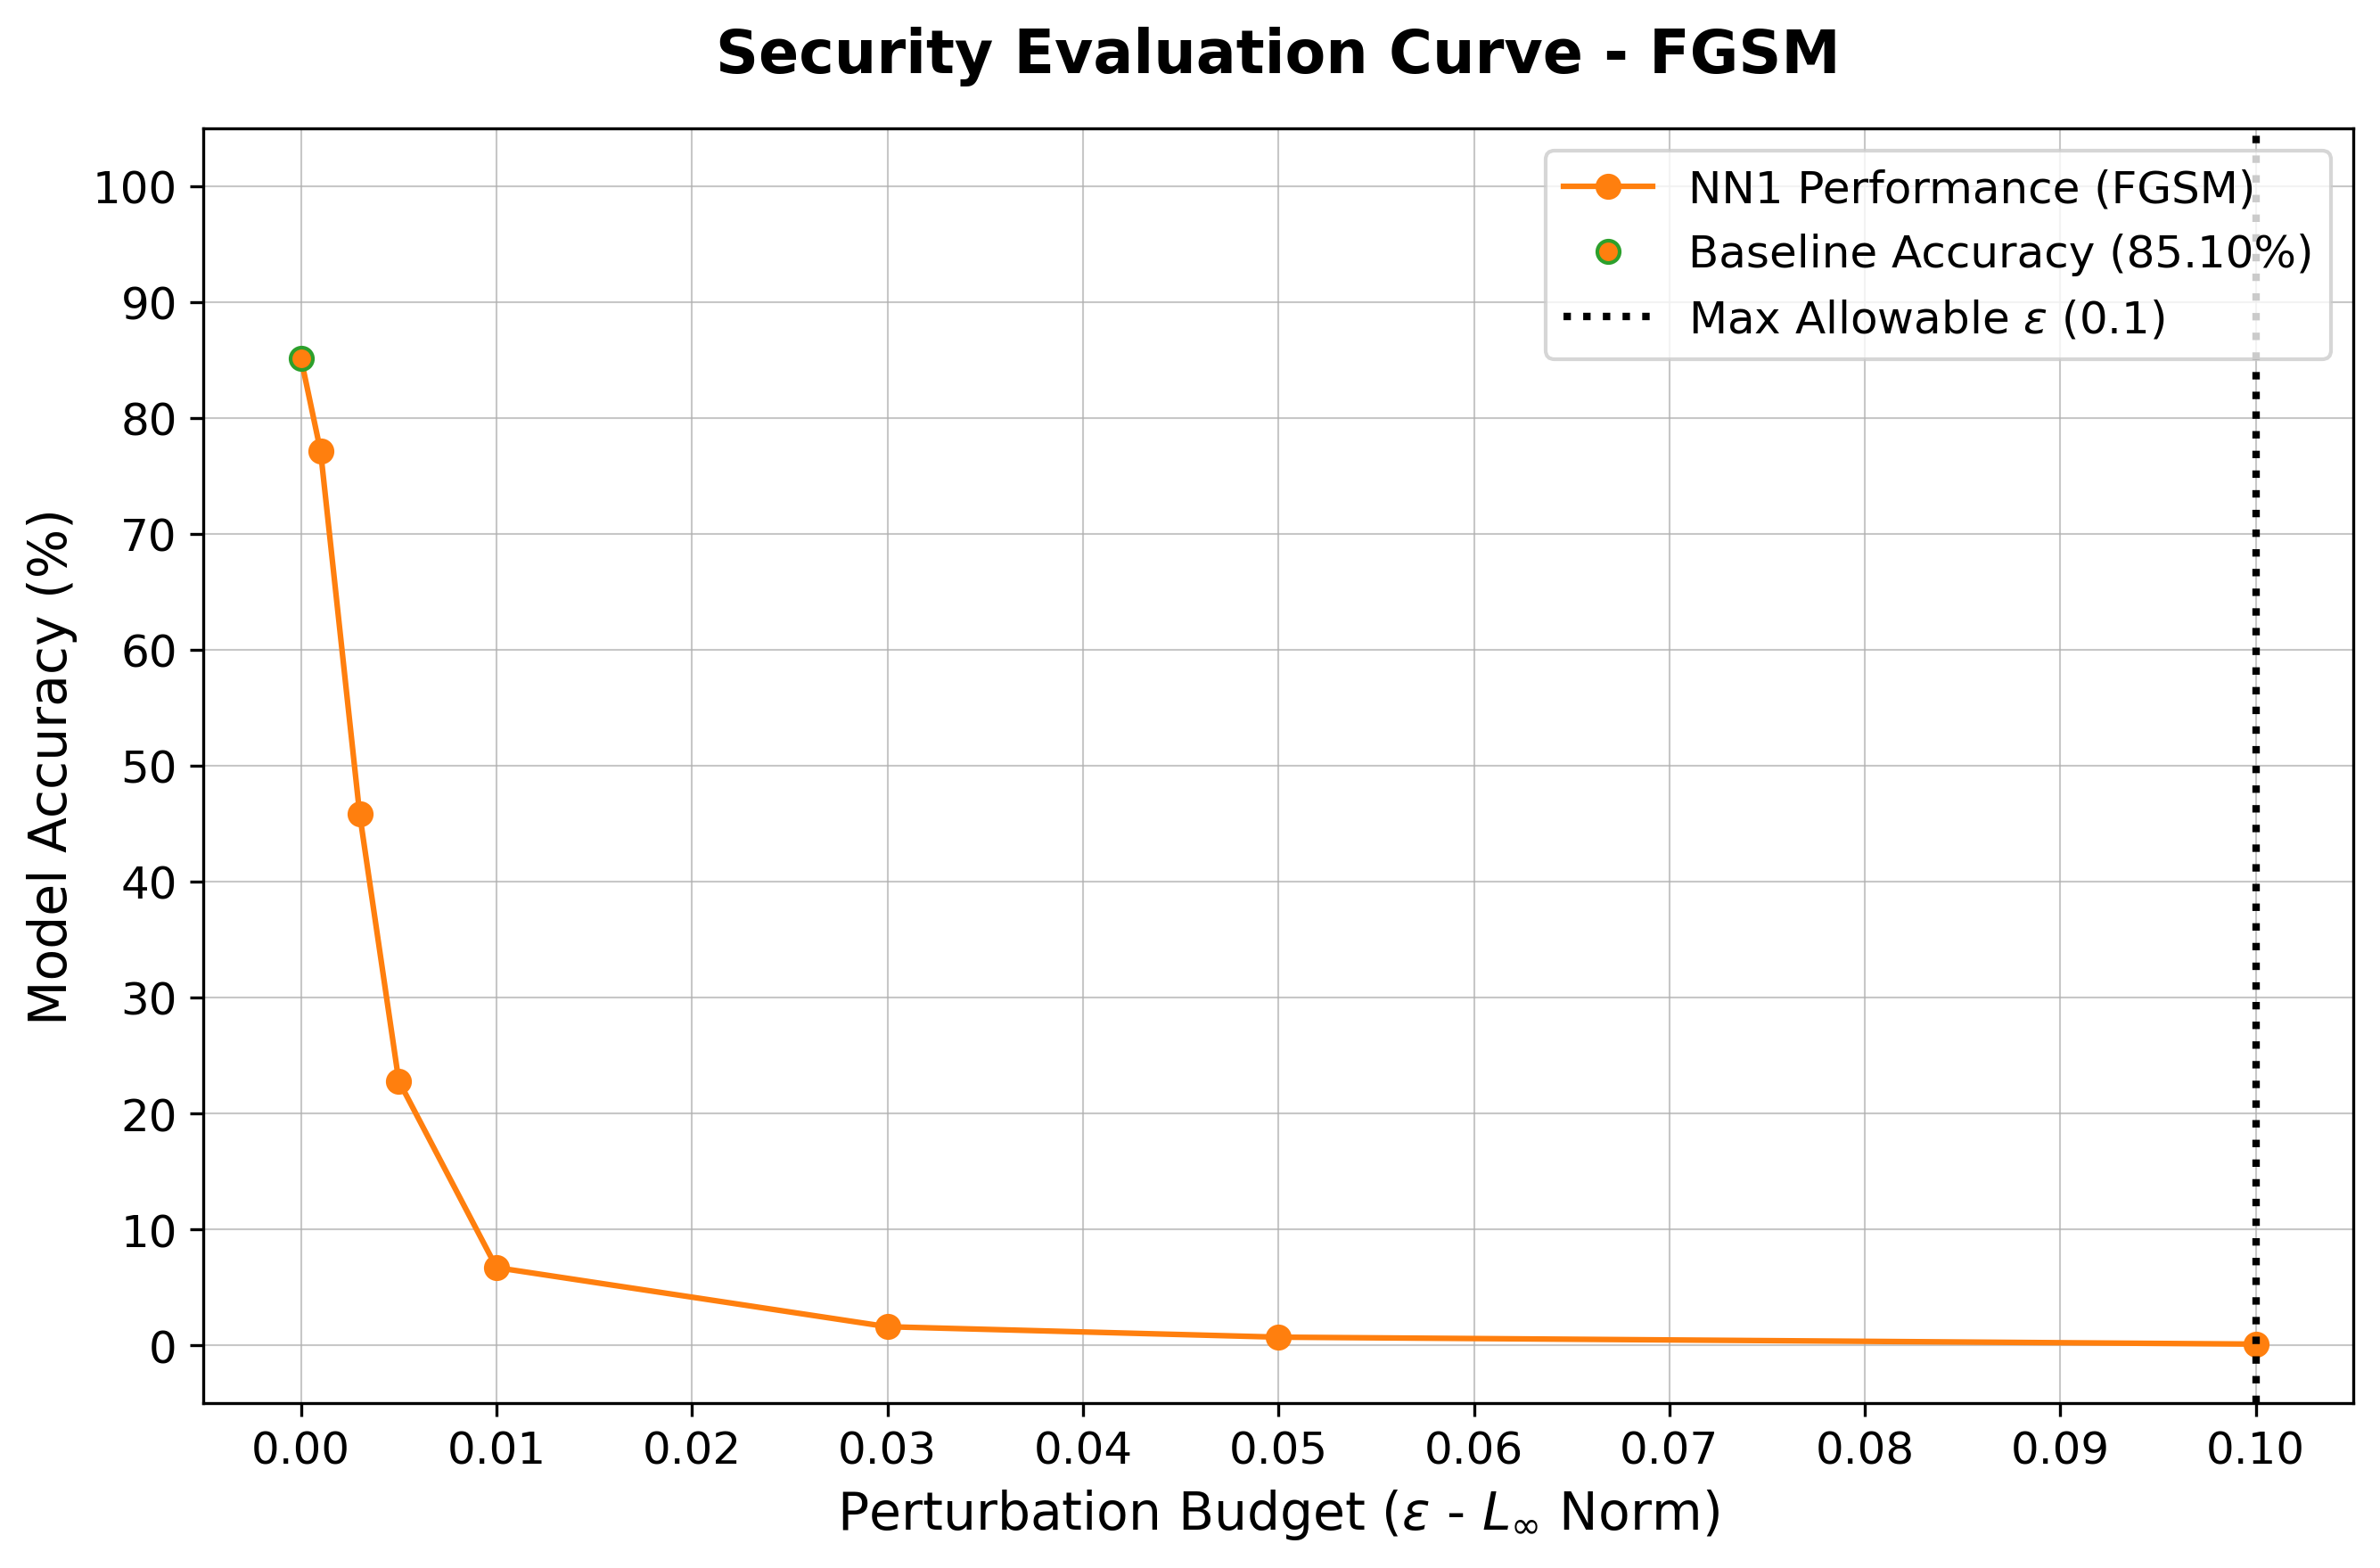
\includegraphics[width=0.9\linewidth]{FGSM/FGSM_SEC.png}
    \caption{FGSM SEC su NN1}
    \label{fig:FGSM_SEC_NN1}
\end{figure}


\begin{table}[H]
    \centering
    \begin{tabular}{ccccc}
        \toprule
        \textbf{$\epsilon$} & \textbf{Correct Predictions} & \textbf{Total Images} & \textbf{Accuracy (\%)} & \textbf{Time (s)} \\
        \midrule
        0.001 & 771 & 1000 & 77.1 & 17.33 \\
        0.003 & 458 & 1000 & 45.8 & 17.27 \\
        0.005 & 228 & 1000 & 22.8 & 22.37 \\
        0.01  & 67  & 1000 & 6.7  & 20.57 \\
        0.03  & 16  & 1000 & 1.6  & 17.95 \\
        0.05  & 7   & 1000 & 0.7  & 16.22 \\
        0.1   & 1   & 1000 & 0.1  & 15.66 \\
        \bottomrule
    \end{tabular}
    \caption{Valutazione di robustezza della rete NN1 al variare di $\epsilon$}
    \label{tab:NN1_robustness}
\end{table}

Come si evince dall'andamento della curva, il modello NN1 mostra una severa vulnerabilità anche a fronte di perturbazioni di entità minima. Partendo da un'accuratezza di \textit{baseline} dell'85.10\% su immagini pulite, l'iniezione di un rumore avversario quasi impercettibile ($\epsilon = 0.001$) causa una prima e contenuta flessione delle prestazioni, portando l'accuratezza al 77.1\%. 

Tuttavia, il collasso predittivo più critico si osserva nel range compreso tra $\epsilon = 0.001$ e $\epsilon = 0.01$. Raggiunta la soglia di $\epsilon = 0.01$, il modello registra il 6.7\% di predizioni corrette. Questo dato indica che un rumore pari ad appena l'1\% della scala dei pixel è sufficiente per ingannare la rete InceptionResnetV1 in oltre il 93\% dei casi.

Per valori di $\epsilon \ge 0.03$, la curva assume un comportamento asintotico tendente allo zero. Al raggiungimento del limite massimo consentito per i test ($\epsilon = 0.1$), l'efficacia del classificatore è di fatto annullata (0.1\%), dimostrando il totale \textbf{successo dell'attacco \textit{error-generic}}.

Infine, l'analisi dei tempi di computazione riportati in Tabella \ref{tab:NN1_robustness} conferma empiricamente la natura dell'algoritmo. Essendo FGSM un metodo \textit{single-step}, il calcolo del gradiente non richiede iterazioni multiple: la generazione di 1000 esempi avversari avviene in un tempo medio compreso tra i 15 e i 22 secondi. Tale efficienza computazionale si mantiene pressoché costante e indipendente dalla magnitudo della perturbazione calcolata.

\clearpage
\subsubsection{Basic Iterative Method (BIM)}
Il \textit{\textbf{Basic Iterative Method}} (BIM), rappresenta un'estensione diretta e più sofisticata del \textit{Fast Gradient Sign Method}. Sviluppato per superare i limiti di precisione degli attacchi \textit{single-step}, BIM applica la perturbazione avversaria attraverso iterazioni multiple e sequenziali, ricalcolando il gradiente ad ogni singolo passaggio per ottimizzare la direzione dell'errore.

In questa valutazione \textit{error-generic}, l'algoritmo non compie un unico sbalzo pari a $\epsilon$. Al contrario, il \textit{budget} di perturbazione totale viene suddiviso in step frazionari di ampiezza minore ($\alpha$), definita spazialmente come $\alpha = \epsilon / \text{max\_iter}$. Formalmente, l'aggiornamento iterativo segue l'equazione:

$$ x'_t = x'_{t-1} + \alpha \cdot \text{sign}(\nabla_x \mathcal{L}(h(x'_{t-1}, w), y)) $$

dove:
\begin{itemize}
    \item $x'_t$: è l'immagine avversaria al passo $t$ (con $x'_0$ pari all'immagine originale pulita);
    \item $\mathcal{L}$: rappresenta la funzione di costo;
    \item $h(\cdot, w)$: la rete neurale target parametrizzata dai pesi $w$.
\end{itemize}

Al termine di ogni step, i valori risultanti subiscono tipicamente un'operazione di \textit{clipping} per garantire che l'immagine alterata rimanga rigorosamente confinata all'interno della sfera $L_\infty$ di raggio $\epsilon$ centrata sull'input di partenza.

Per analizzare in modo approfondito e granulare la vulnerabilità della rete NN1 a questo attacco, l'architettura di test è stata espansa su due dimensioni parametriche (\texttt{EPSILON} e \texttt{MAX_ITER_LIST}). Quindi il processo di generazione non si è limitato a iterare sullo spettro di valori di $\epsilon$ da 0.001 a 0.1, ma per ciascun \textit{budget} ha valutato diverse iterazioni, testando l'algoritmo per: 
\begin{verbatim}
MAX_ITER_LIST = [1, 5, 10, 20]
EPSILON = [0.001, 0.003, 0.005, 0.01, 0.03, 0.05, 0.1]

\end{verbatim}

Questo spazzolamento bidimensionale ha consentito la generazione di un set di \textit{Security Evaluation Curve} (SEC) individuali per ogni limite iterativo, nonché di una curva SEC comparativa che sovrappone le diverse configurazioni. Inoltre, al fine di isolare l'efficacia del parametro iterativo, è stato tracciato un grafico dedicato all'effetto degli iperparametri, che osserva la caduta di accuratezza in funzione esclusiva del numero di step (\texttt{max\_iter}) a fronte di tre soglie fisse di $\epsilon$ (0.01, 0.05 e 0.1). 

Nelle sezioni seguenti vengono analizzati nel dettaglio i risultati quantitativi e i grafici prodotti da questa matrice di valutazione.

\begin{figure}[H]
    \centering
    % Sotto-figura 1
    \begin{subfigure}[b]{0.45\textwidth}
        \centering
        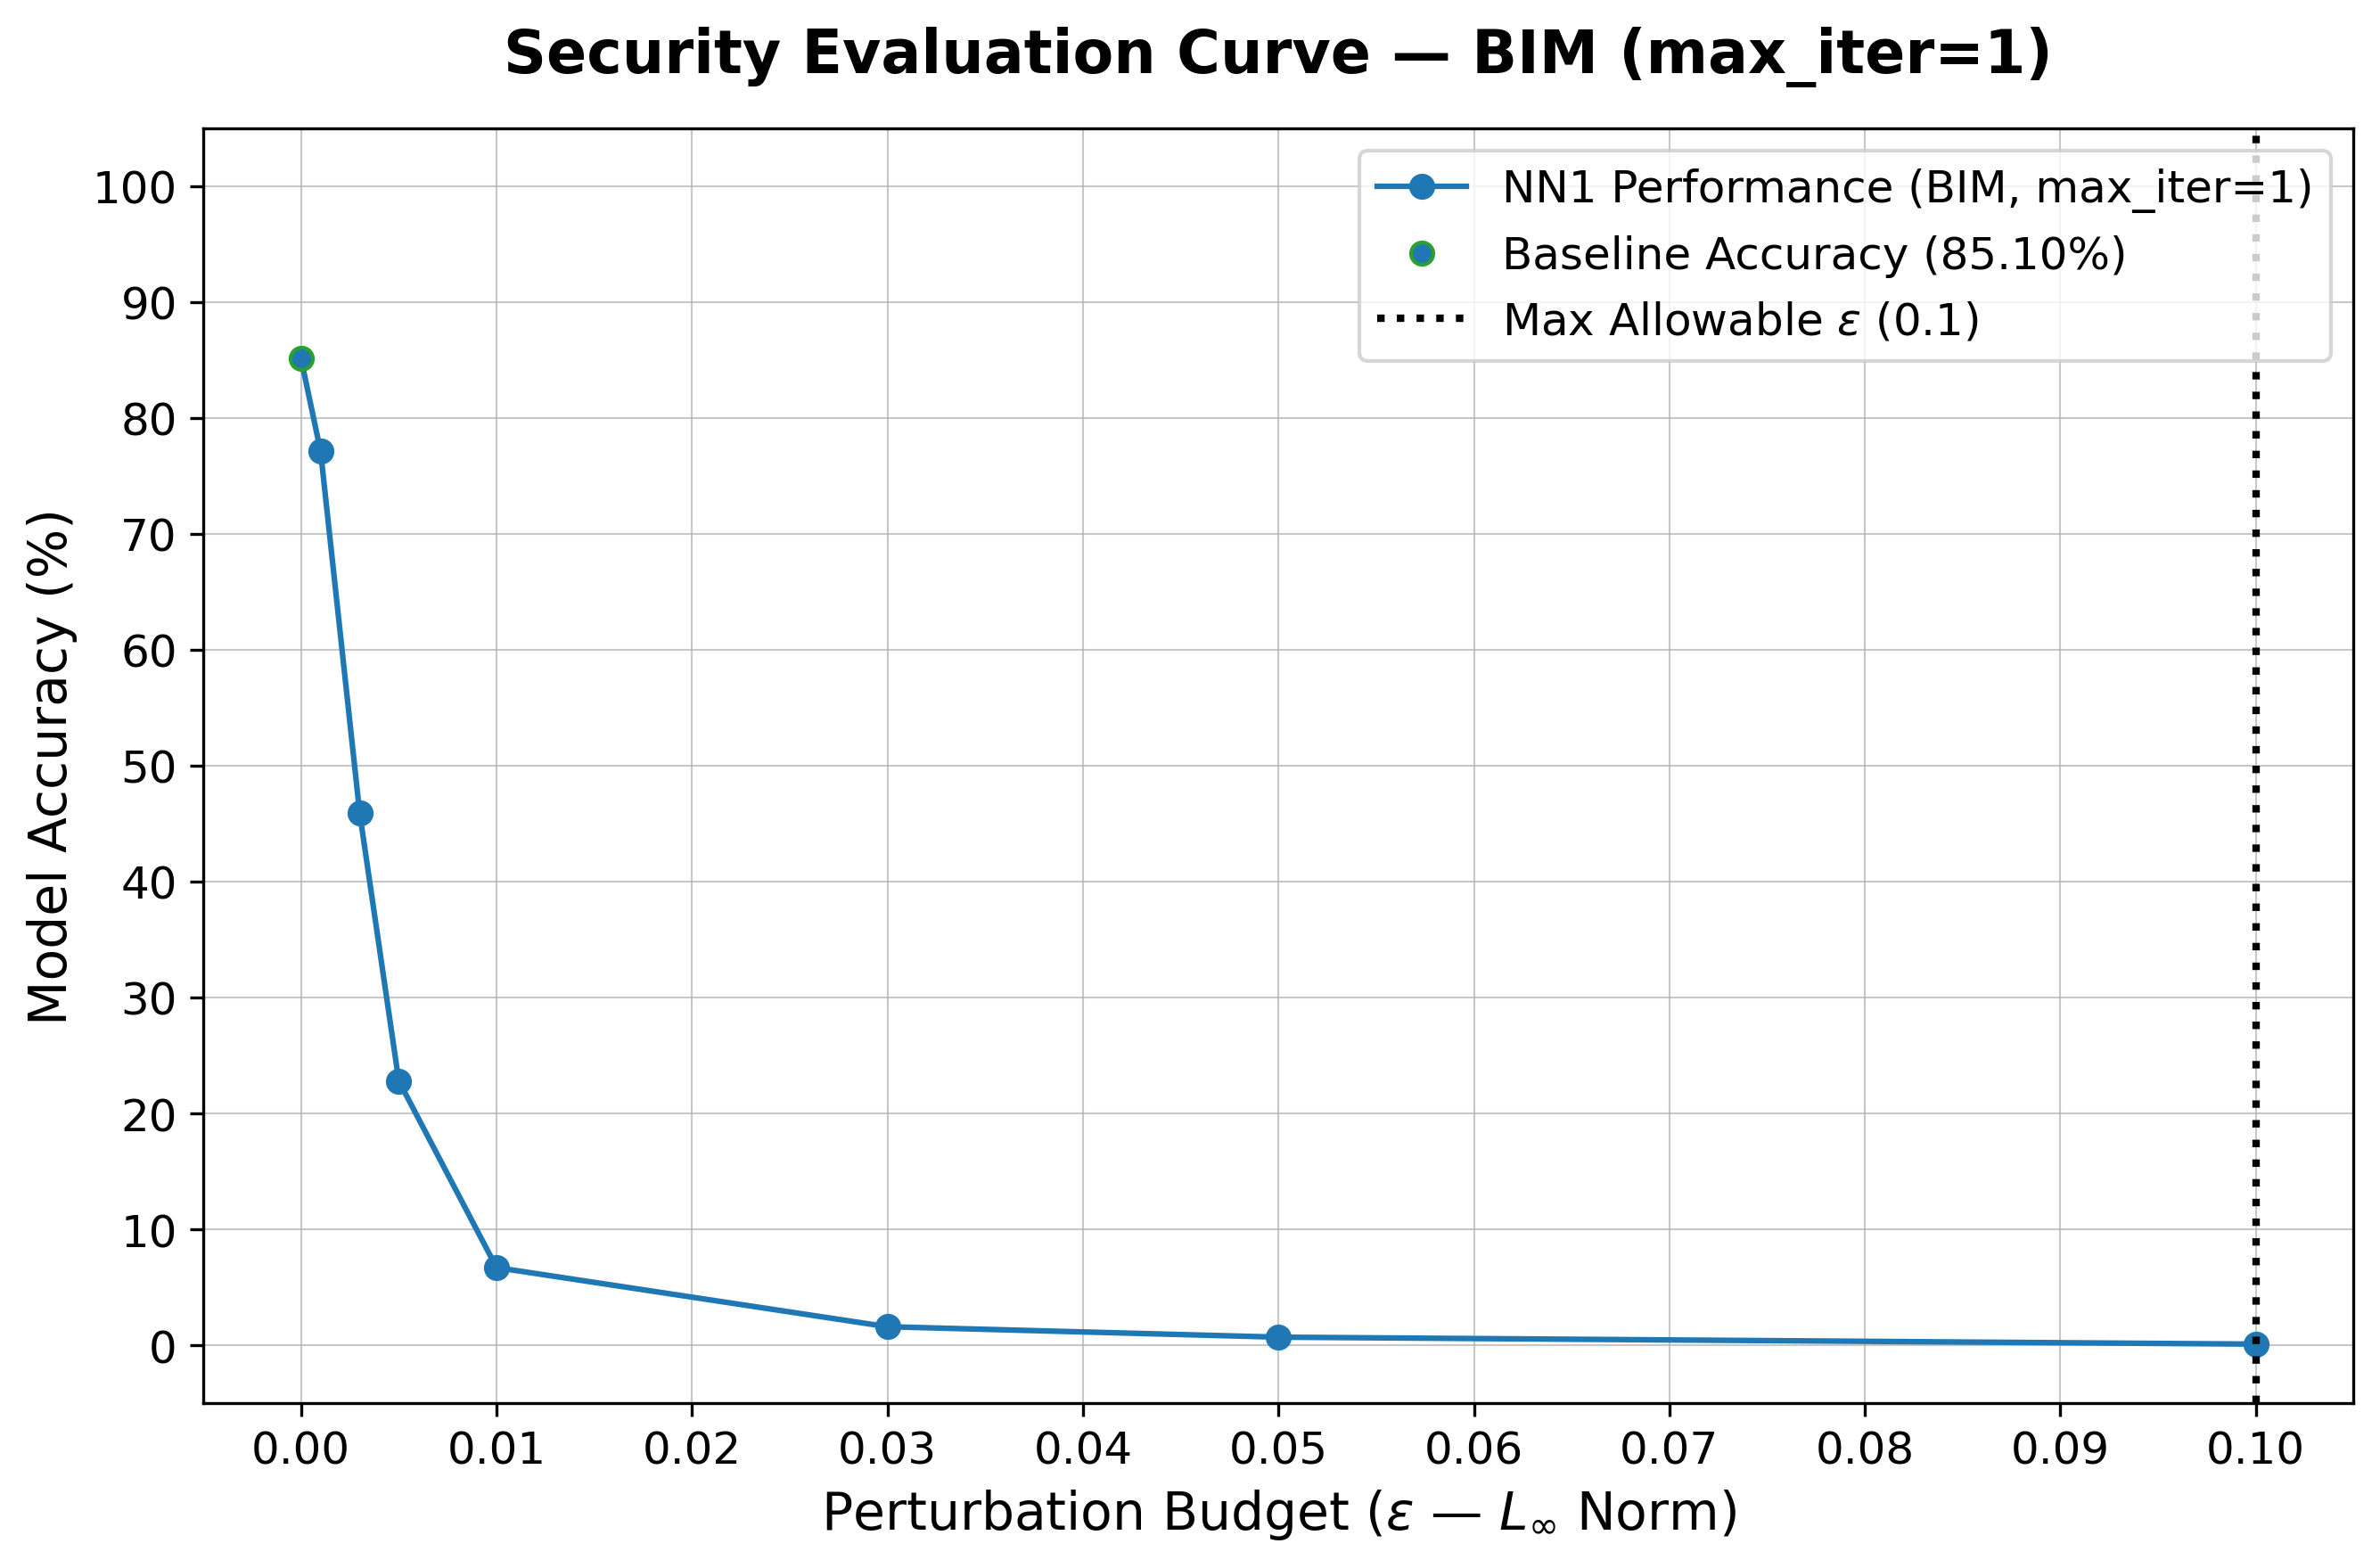
\includegraphics[width=\textwidth]{BIM_Error_generic/BIM_iter1_SEC.png}
        \caption{\texttt{max_iter} = 1}
        \label{fig:iter1}
    \end{subfigure}
    \hfill
    % Sotto-figura 2
    \begin{subfigure}[b]{0.45\textwidth}
        \centering
        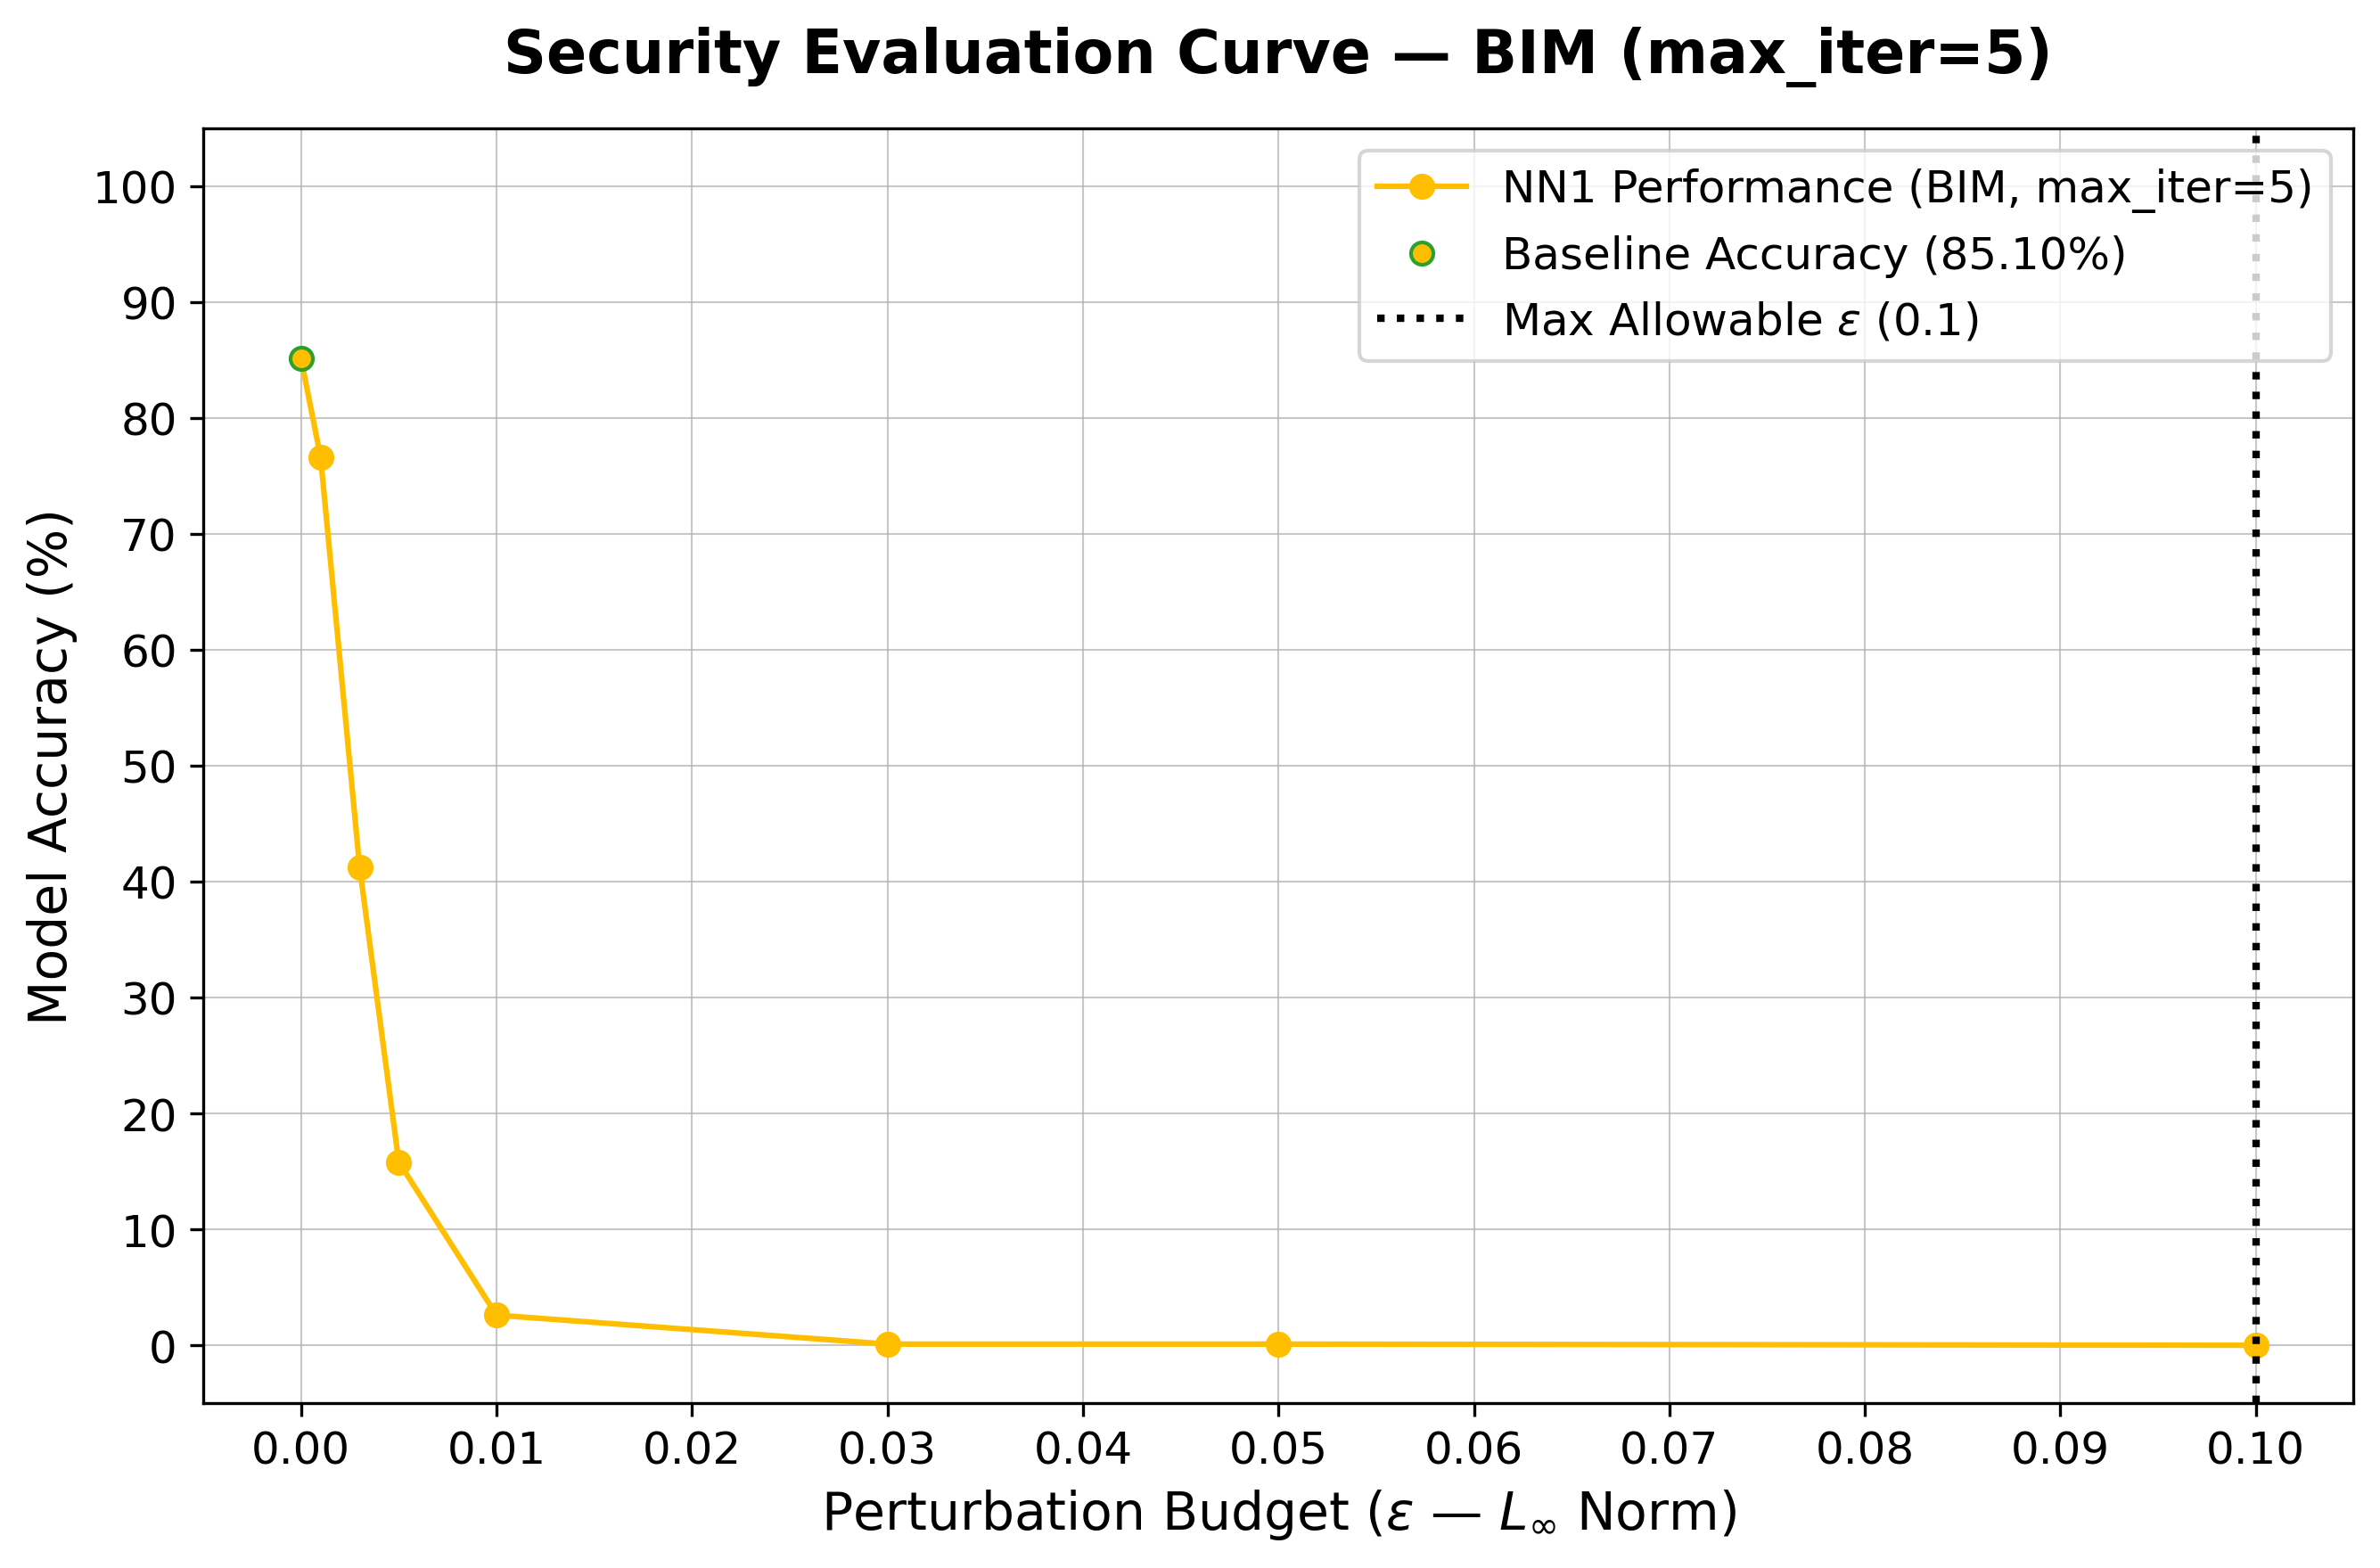
\includegraphics[width=\textwidth]{BIM_Error_generic/BIM_iter5_SEC.png}
        \caption{\texttt{max_iter} = 5}
        \label{fig:iter5}
    \end{subfigure}

    \vspace{1em} % Spazio verticale tra le righe di immagini

    % Sotto-figura 3
    \begin{subfigure}[b]{0.45\textwidth}
        \centering
        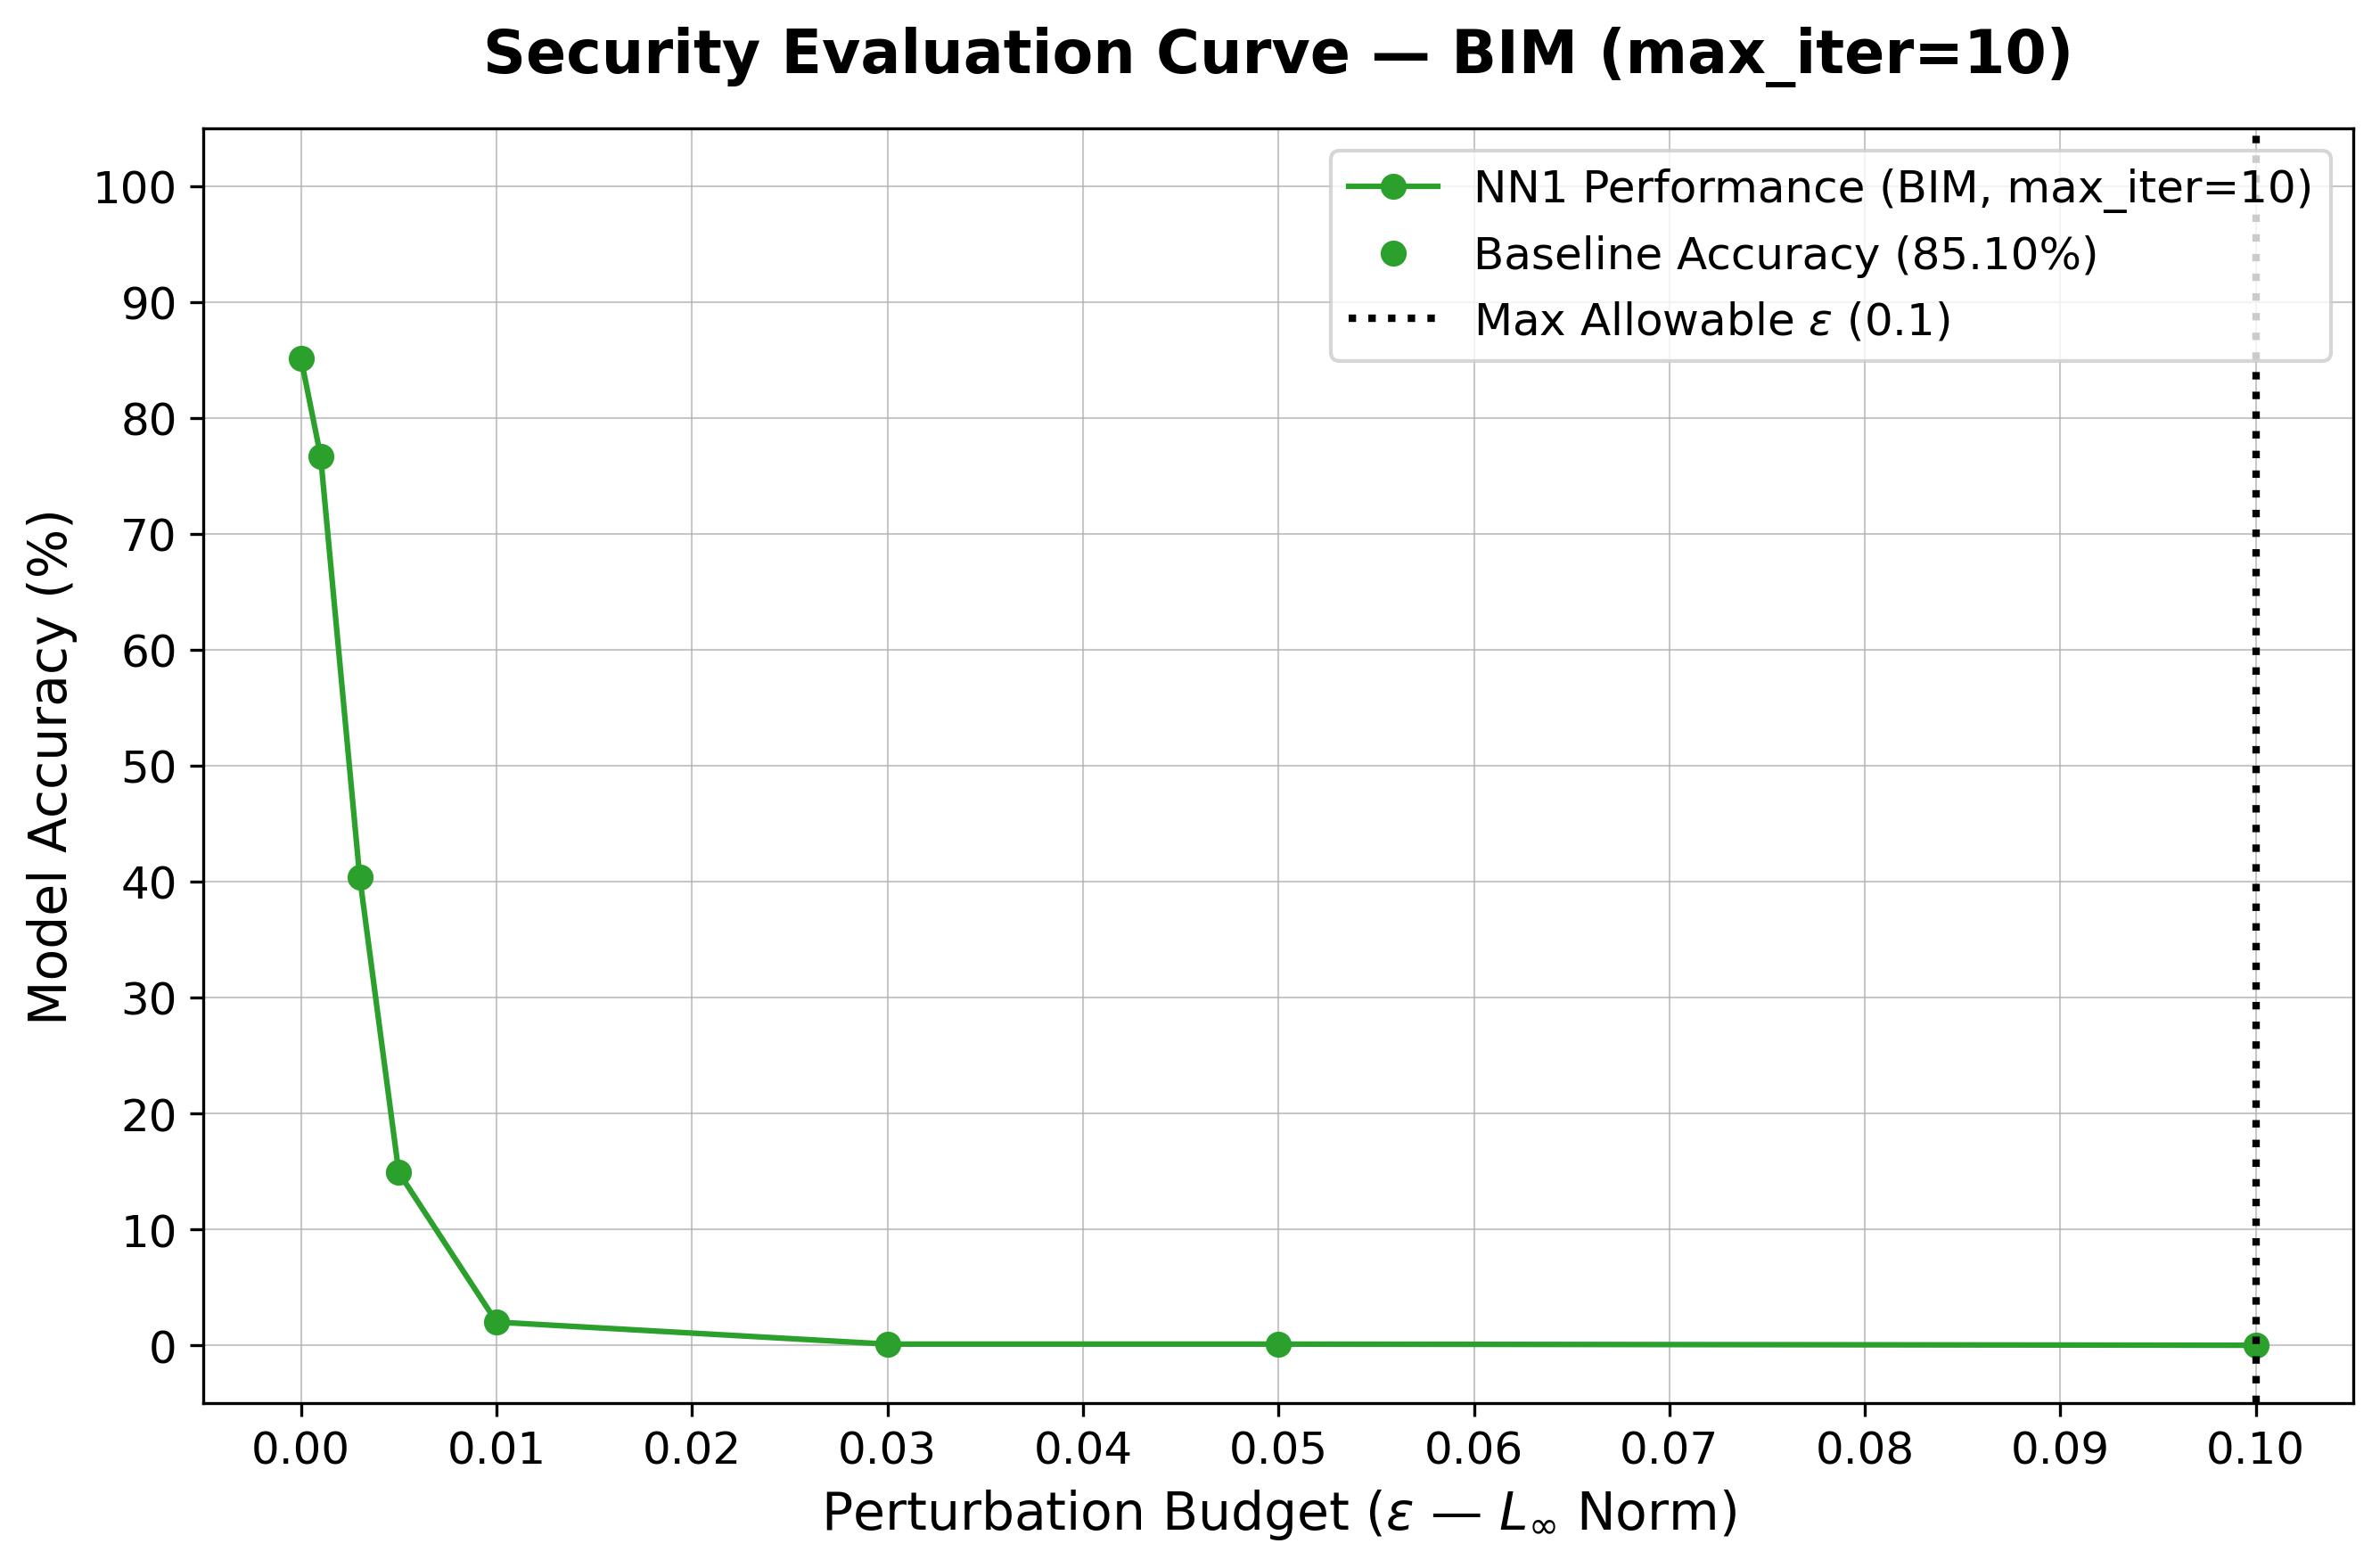
\includegraphics[width=\textwidth]{BIM_Error_generic/BIM_iter10_SEC.png}
        \caption{\texttt{max_iter} = 10}
        \label{fig:iter10}
    \end{subfigure}
    \hfill
    % Sotto-figura 4
    \begin{subfigure}[b]{0.45\textwidth}
        \centering
        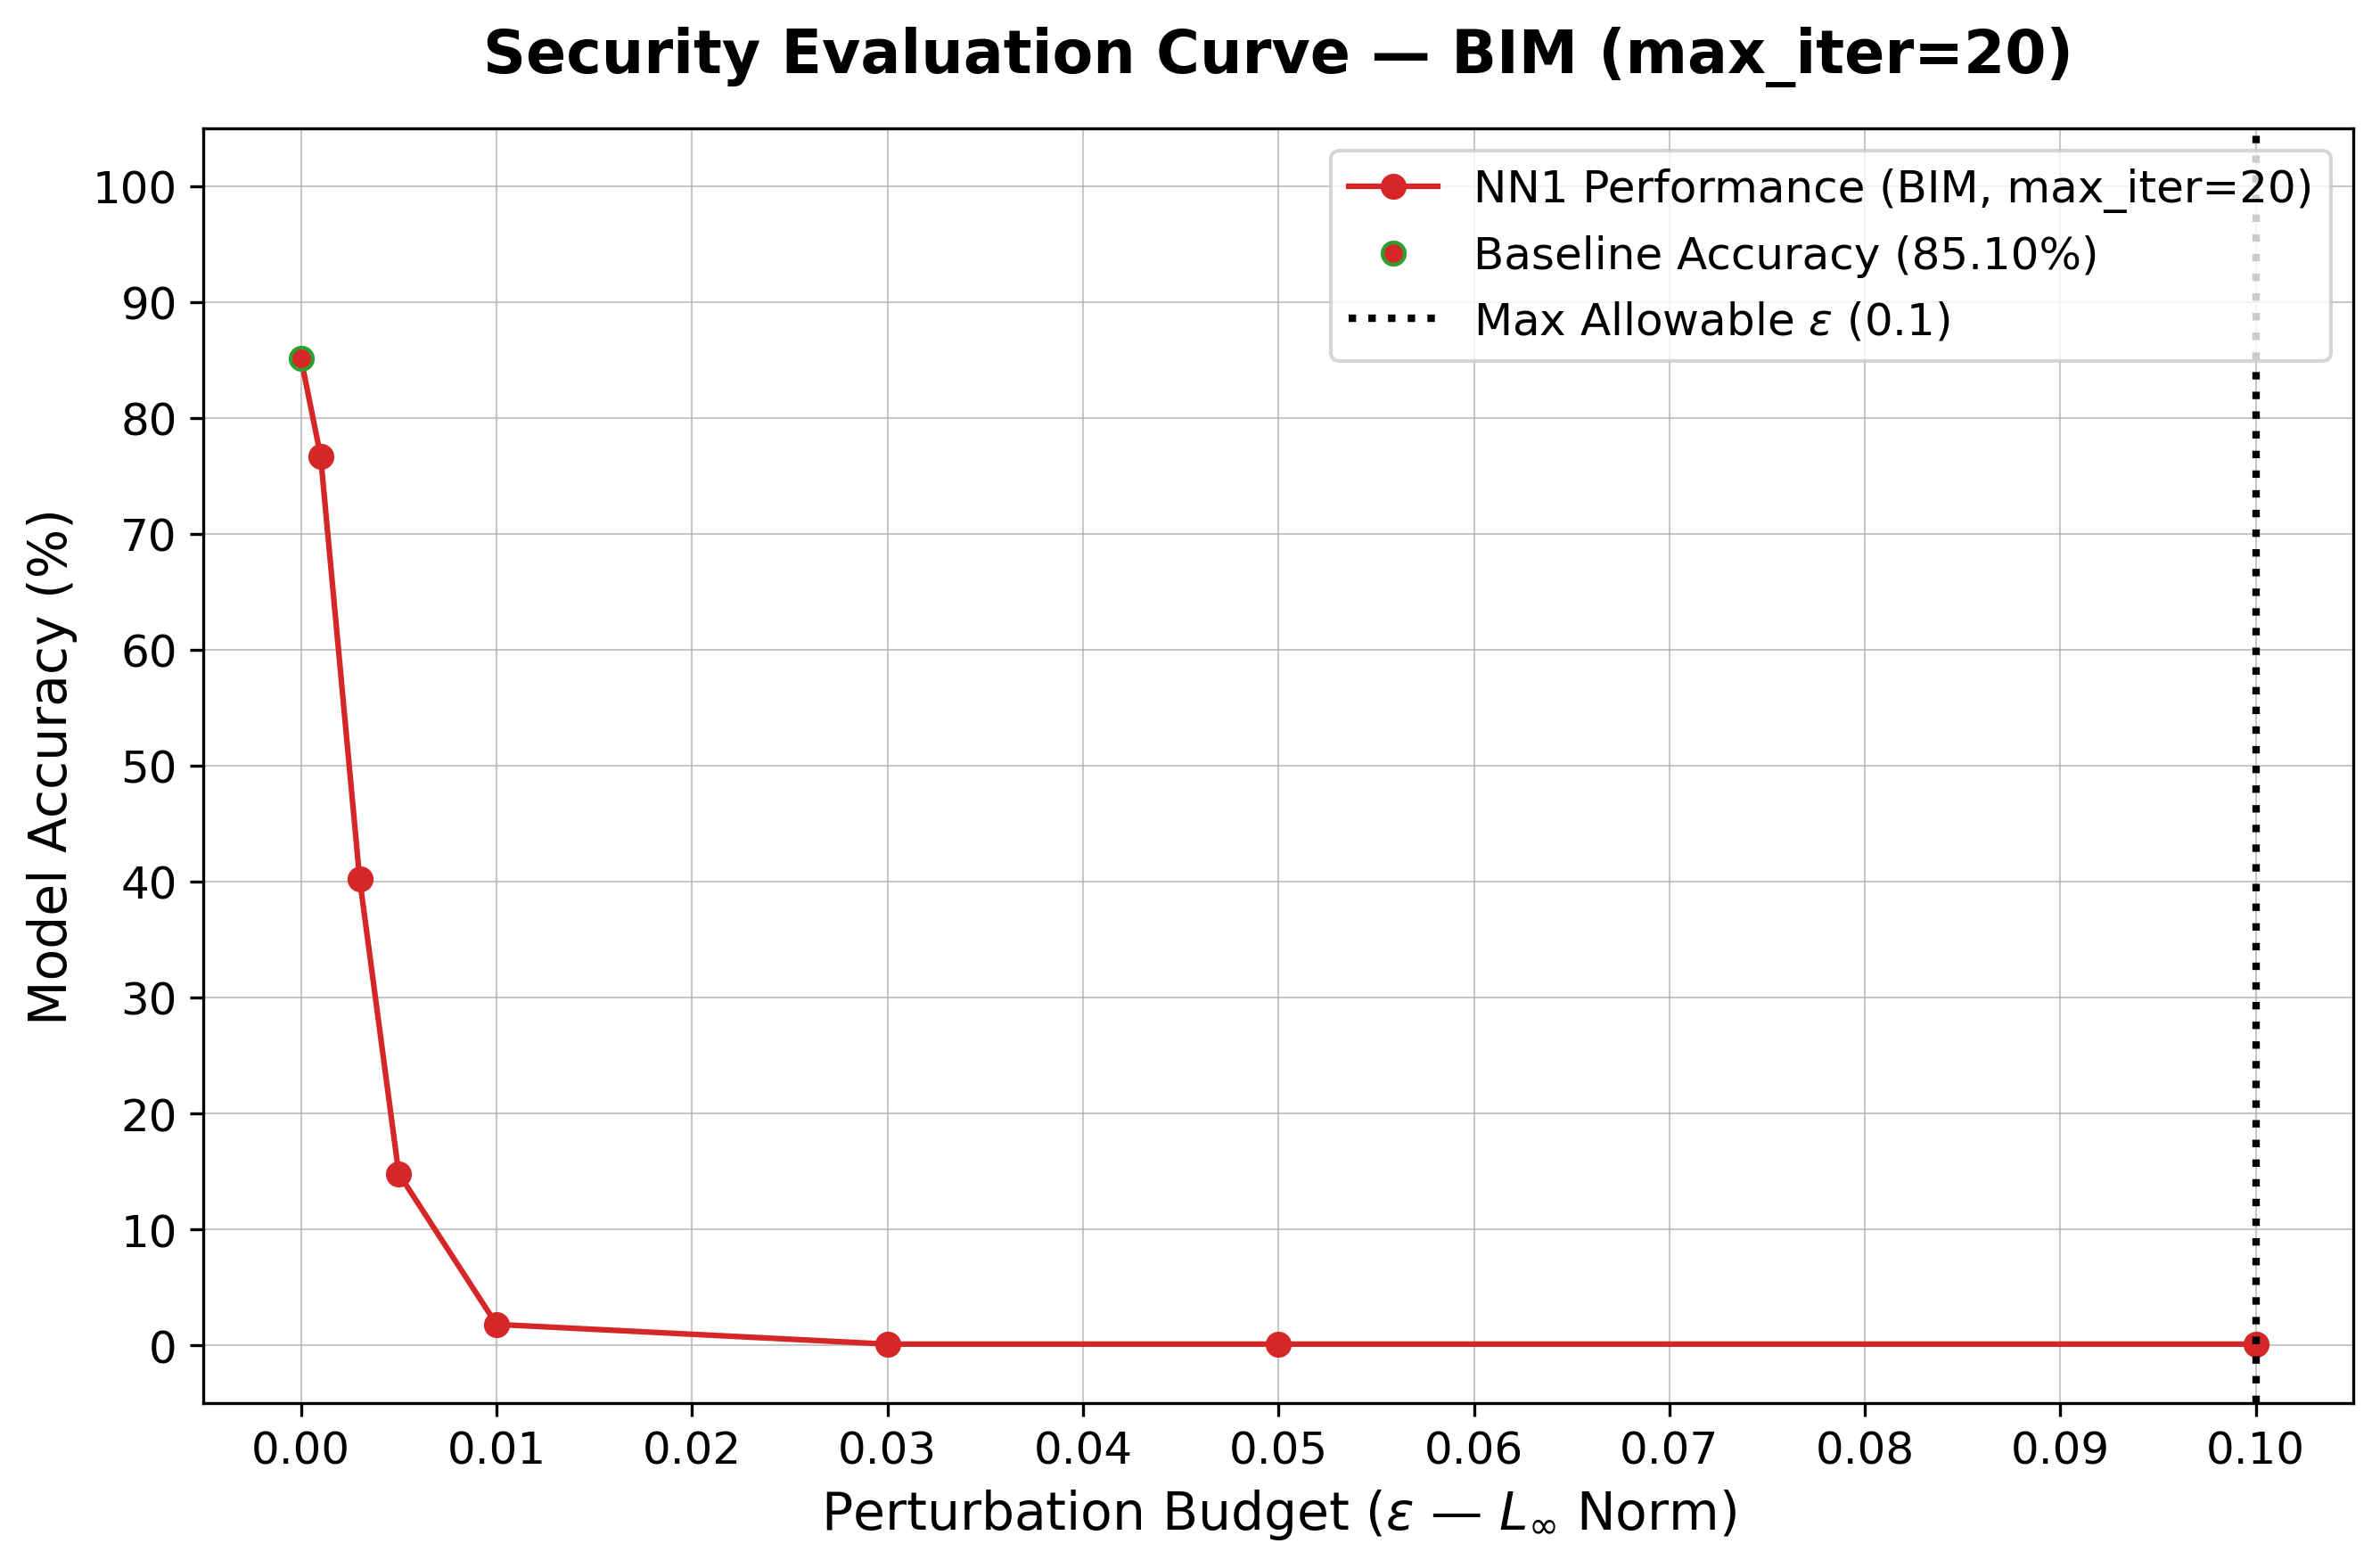
\includegraphics[width=\textwidth]{BIM_Error_generic/BIM_iter20_SEC.png}
        \caption{\texttt{max_iter} = 20}
        \label{fig:iter20}
    \end{subfigure}

    \caption{Visualizzazione delle immagini avversarie al variare del numero di iterazioni.}
    \label{fig:BIM_iterations}
\end{figure}

Per una migliore analisi comparativa, in figura~\ref{fig:BIM_SEC_NN1} è possibile visualizzare la SEC prodotta da BIM sul modello NN1. 

\begin{figure}[h]
    \centering
    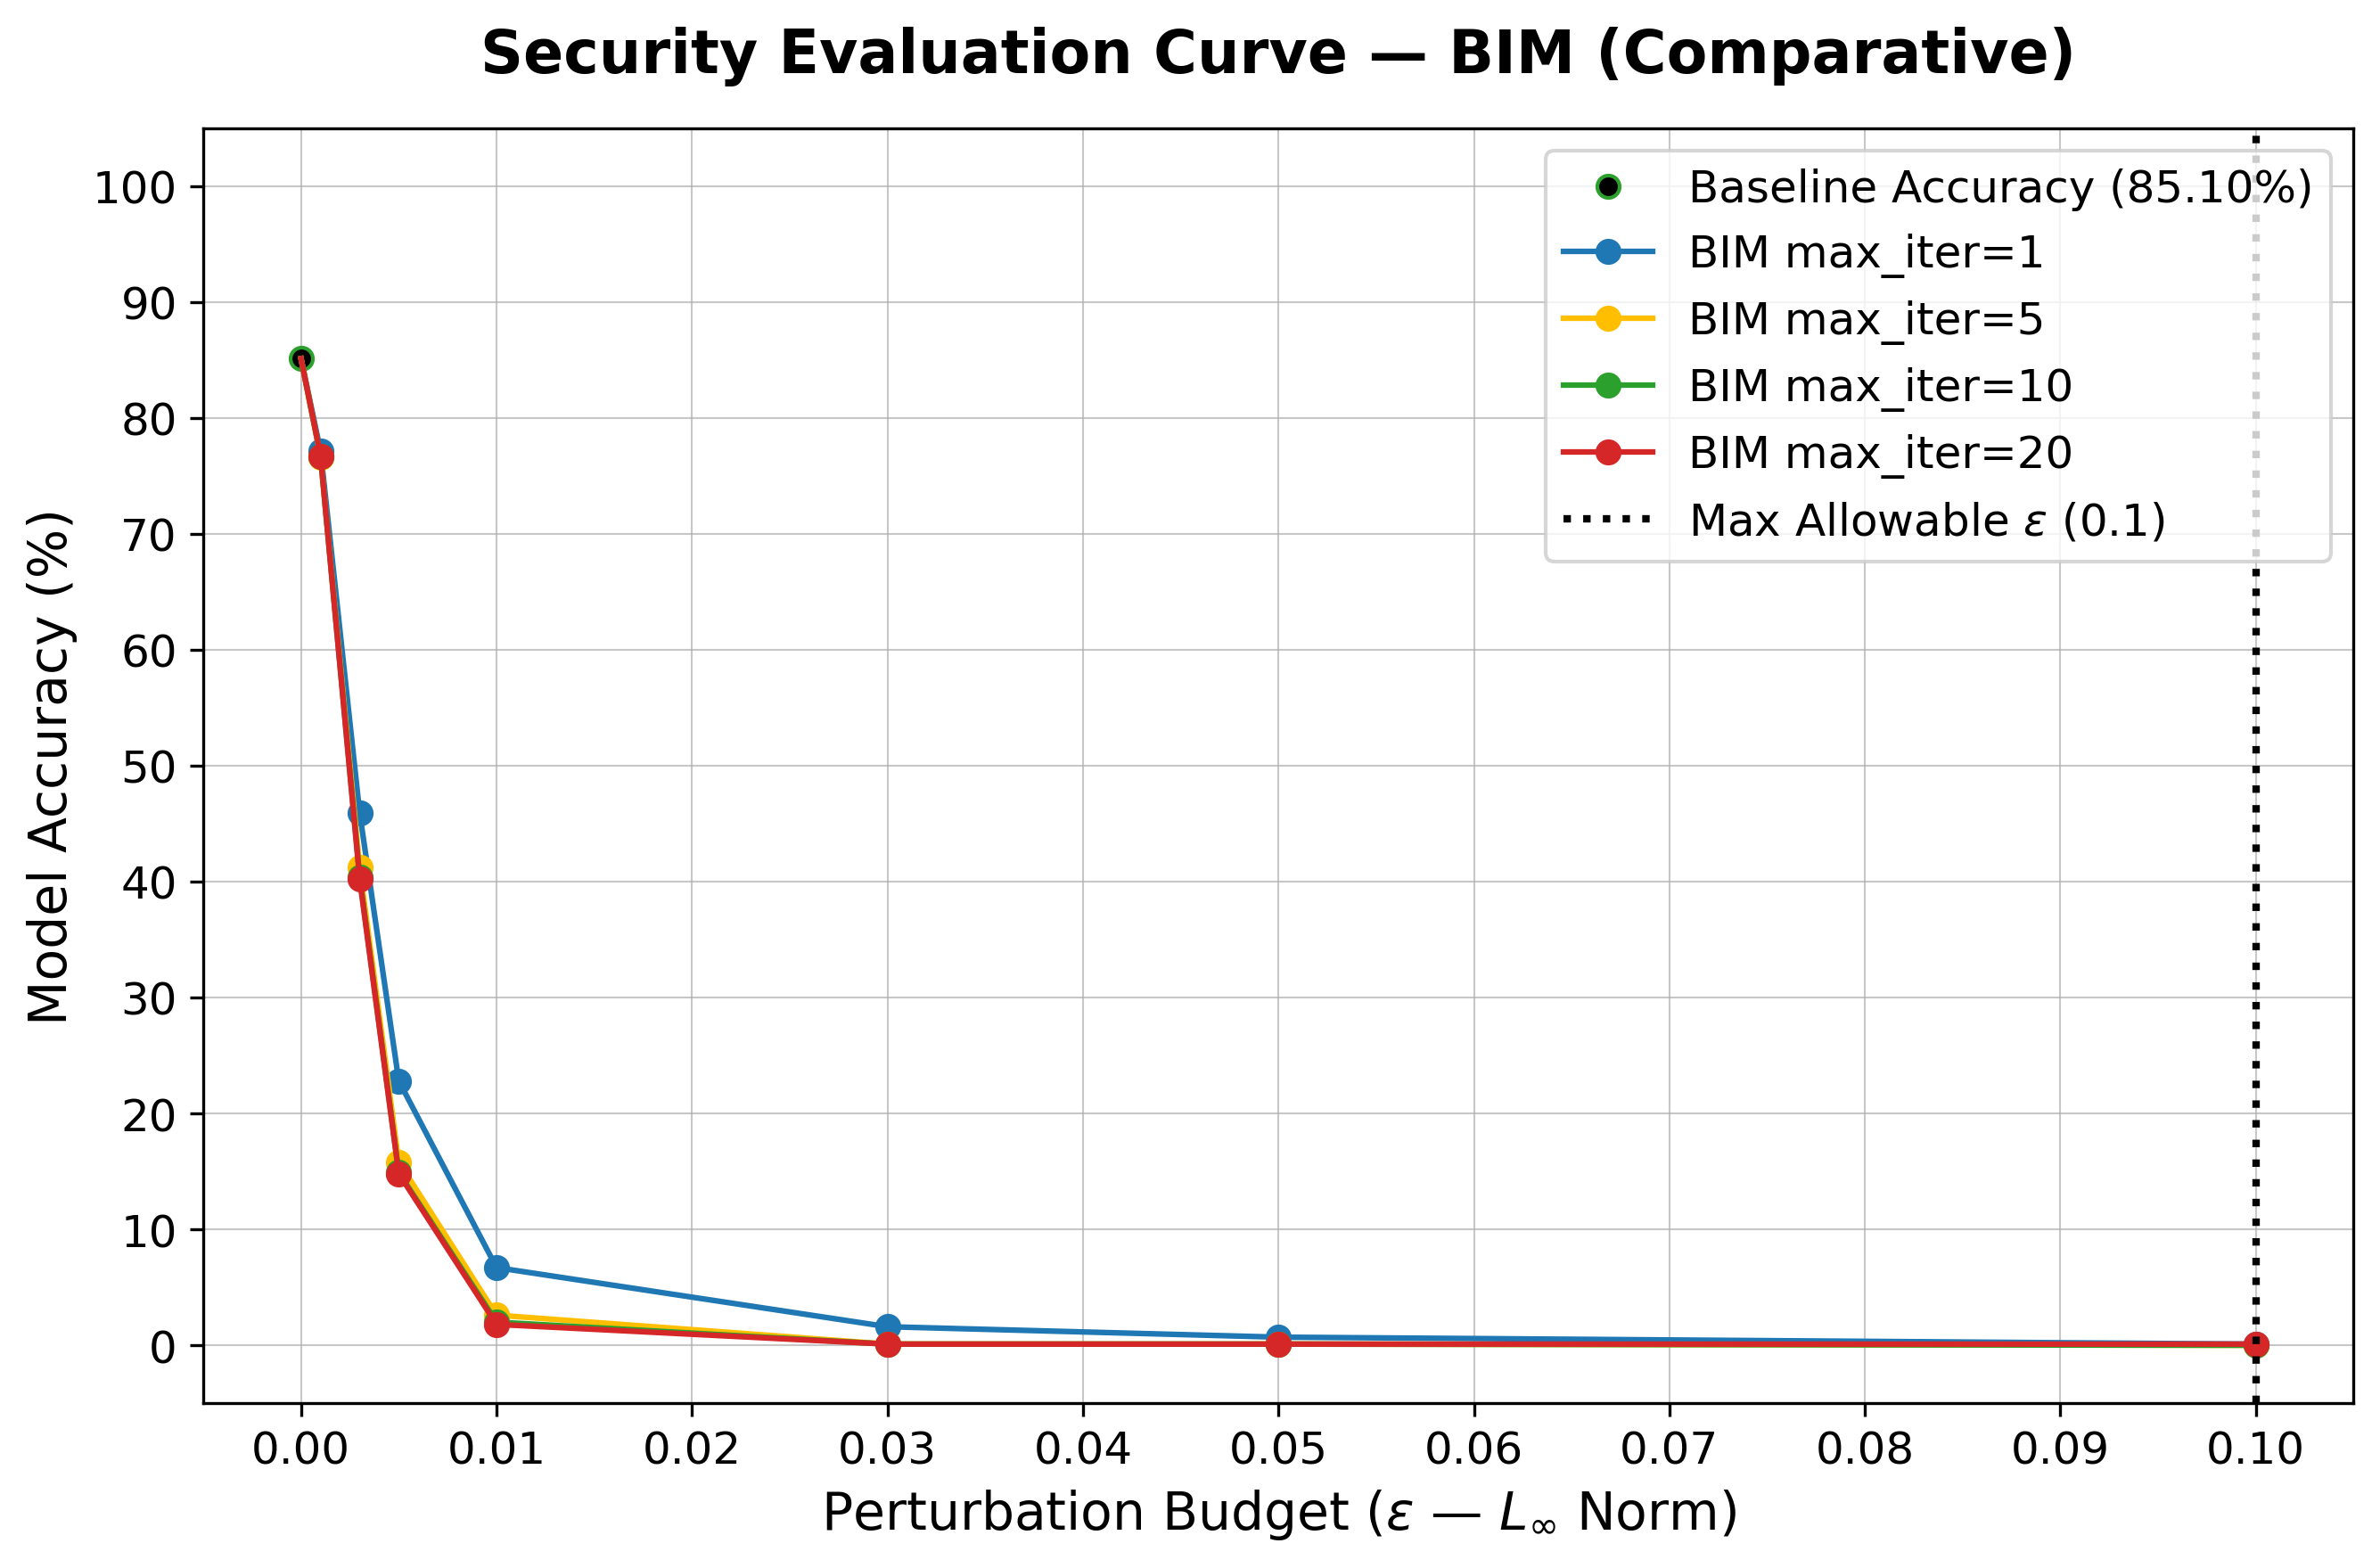
\includegraphics[width=0.75\linewidth]{BIM_Error_generic/BIM_comparative_SEC.png}
    \caption{BIM SEC su NN1}
    \label{fig:BIM_SEC_NN1}
\end{figure}

L'analisi congiunta della curva comparativa (Figura~\ref{fig:BIM_SEC_NN1}) e dei dati quantitativi raccolti durante i test (vedere la cartella al percorso \texttt{results/BIM/BIM_results.csv}) rivela dinamiche tipiche dell'attacco BIM, evidenziando in modo chiaro il vantaggio e i limiti dell'approccio iterativo rispetto alla variante \textit{single-step} (FGSM).
\\
Il primo dato significativo emerge confrontando le curve a parità di budget di perturbazione ($\epsilon$). L'esecuzione con \texttt{max\_iter} = 1 equivale concettualmente a un attacco FGSM tradizionale: tutto il rumore viene calcolato e applicato in un singolo passaggio. In questa configurazione, con $\epsilon$ pari a 0.01, il modello NN1 conserva un'accuratezza del 6.7\%. 
Tuttavia, suddividendo il medesimo budget in 5 step iterativi (\texttt{max\_iter} = 5), l'algoritmo riesce a ricalcolare il gradiente man mano che l'immagine si sposta nello spazio delle feature, ottimizzando la direzione del rumore. Questa maggiore precisione fa diminuire l'accuratezza al 2.6\%, dimostrando che l'approccio multi-step è più distruttivo, pur non alterando il budget.
\\
Osservando la Figura~\ref{fig:BIM_SEC_NN1}, è visibile come lo scarto prestazionale tra le diverse configurazioni non sia lineare. Si nota un netto distacco tra la curva blu (1 iterazione) e la curva gialla (5 iterazioni), ma all'aumentare ulteriore degli step (10 e 20 iterazioni) le curve tendono a sovrapporsi, indicando un fenomeno di saturazione.
I dati confermano visivamente questa tendenza: sempre prendendo come riferimento $\epsilon$ = 0.01, il passaggio da 10 a 20 iterazioni non produce alcun degrado aggiuntivo apprezzabile. L'algoritmo raggiunge quindi il suo massimo potenziale offensivo già intorno al budget $\epsilon$ = 0.05 ; frammentare ulteriormente il parametro apporta benefici marginali.  

\clearpage
\subsubsection{Projected Gradient Descent (PGD)}
Il \textit{\textbf{Projected Gradient Descent}} (PGD) rappresenta una naturale evoluzione del \textit{Basic Iterative Method} (BIM), dal quale eredita la struttura computazionale multi-step, introducendo tuttavia un elemento stocastico cruciale: l'inizializzazione casuale (\textit{random restart}).

Mentre BIM inizia l'ottimizzazione del gradiente partendo sempre dall'immagine originale pulita, PGD perturba il punto di partenza aggiungendo un rumore casuale campionato uniformemente all'interno della sfera $L_\infty$ di raggio $\epsilon$. Questa perturbazione iniziale permette all'algoritmo di esplorare porzioni diverse del paesaggio della funzione di costo (\textit{loss landscape}), riducendo drasticamente il rischio di convergere in un massimo locale sub-ottimale. 

Formalmente, l'algoritmo si articola in due fasi. La prima prevede l'inizializzazione stocastica, ovvero la primissima fase in cui viene applicata una perturbazione casuale campionata da una distribuzione uniforme con valori nel range $(-\epsilon,\epsilon)$:
$$ x'_0 = x + \eta \quad \text{con} \quad \eta \sim \mathcal{U}(-\epsilon, \epsilon) $$

Successivamente, si applica l'aggiornamento iterativo basato sul gradiente, regolato dall'operazione di proiezione:
$$ x'_t = \Pi_\epsilon \left( x_{t-1} + \alpha \cdot \text{sign}(\nabla_x \mathcal{L}(h(x_{t-1}, w), y)) \right) $$

dove:
\begin{itemize}
    \item $\Pi_\epsilon$ rappresenta l'operatore di proiezione, il quale garantisce che ad ogni step l'immagine alterata rimanga rigorosamente confinata all'interno dell'intorno $L_\infty$ di raggio $\epsilon$ centrato sull'input originale $x$;
    \item $\mathcal{L}$ è la funzione di costo valutata sulla rete neurale target $h$ (parametrizzata dai pesi $w$) rispetto all'etichetta reale $y$;
    \item $\alpha = \epsilon / \text{max\_iter}$ definisce l'ampiezza del passo per la singola iterazione.
\end{itemize}

\textbf{Se la rete neurale viene ingannata con successo durante uno qualsiasi dei riavvii casuali, l'attacco viene considerato riuscito. ????????}

Per valutare in modo esaustivo la robustezza della rete NN1 contro questo attacco \textit{error-generic}, l'architettura di test implementata è stata strutturata su una complessa matrice tridimensionale. Oltre a spaziare sul budget di perturbazione $\epsilon$ (da 0.001 a 0.1) e sulla profondità computazionale \texttt{max\_iter} (1, 5, 10, 20 e 40 step), è stata introdotta la variabile \texttt{num\_random\_init}, valutata per i valori 0, 1, 3 e 5:

\begin{verbatim}
EPSILONS           = [0.001, 0.003, 0.005, 0.01, 0.03, 0.05, 0.1]
MAX_ITER_LIST      = [1, 5, 10, 20, 40]
NUM_RANDOM_INITS   = [0, 1, 3, 5]

\end{verbatim}

È fondamentale sottolineare che la configurazione con \texttt{num\_random\_init} = 0 disabilita la componente stocastica, riducendo di fatto PGD a un attacco BIM standard. Questo espediente metodologico fornisce una \textit{baseline} algoritmica perfetta per isolare e quantificare il reale valore aggiunto dei \textit{random restart}.

L'esecuzione di questa vasta mole di permutazioni ha generato un set stratificato di \textit{Security Evaluation Curve} (SEC). Nelle sezioni successive verranno analizzati i risultati quantitativi, esplorando l'impatto isolato delle iterazioni (\textit{ceteris paribus} rispetto ai riavvii casuali) e l'efficacia dei \textit{random restart} (\textit{ceteris paribus} rispetto alle iterazioni).

\textbf{AGGIUNGERE I GRAFICI E L'ANALISI PER PGD}

L'analisi quantitativa, i cui risultati compatti sono visibili nelle \textit{Security Evaluation Curve} (SEC) prodotte e nei dati estratti dal file CSV, evidenzia in primo luogo l'estrema vulnerabilità della rete agli attacchi iterativi non mirati. Già con \texttt{max\_iter} = 5 e un budget minimo di $\epsilon = 0.03$, l'algoritmo (sia esso stocastico o deterministico) raggiunge un ASR pressoché totale (oltre il 99.8\%), saturando le difese del modello.

Il dato scientificamente più rilevante emerge tuttavia dall'analisi incrociata del parametro \texttt{num\_random\_init}. A livello teorico, l'inizializzazione stocastica di PGD è concepita per eludere i minimi locali della funzione di costo, suggerendo prestazioni pari o superiori alla variante deterministica (BIM, equivalente a \texttt{nri} = 0). Sorprendentemente, il test su questo dominio smentisce tale assunzione portando a dei risultati lievemente migliori per BIM.

Focalizzando l'attenzione sui valori di \textit{budget} inferiori, dove la saturazione dell'errore non maschera le differenze algoritmiche (es. $\epsilon = 0.01$), si osserva un degrado sistematico delle performance all'aumentare dei riavvii casuali. Ad esempio, eseguendo 10 iterazioni con $\epsilon = 0.01$, l'approccio BIM (\texttt{nri} = 0) riesce a distruggere la predizione nel 98.0\% dei casi (lasciando un'accuratezza residua del 2.0\%). Al contrario, armando PGD con 5 \textit{random restart} a parità di iterazioni, l'ASR scende al 95.9\% (accuratezza residua del 4.1\%). Questa dinamica di lieve decremento offensivo si conferma per tutte le configurazioni iterative (\texttt{max\_iter} da 1 a 40).

\clearpage
\subsubsection{Carlini \& Wagner (CW)}
L'algoritmo di Carlini \& Wagner (CW) rappresenta uno degli attacchi avversari più sofisticati e potenti presenti in letteratura. A differenza dei metodi analizzati in precedenza (basati sul segno del gradiente computato in uno o più step temporali), CW riformula la generazione dell'esempio avversario come un vero e proprio problema di ottimizzazione continua. L'algoritmo non cerca di massimizzare l'errore dato un budget, ma al contrario cerca di minimizzare la perturbazione garantendo l'inganno del classificatore.

La formulazione generale dell'algoritmo si esprime come un problema di minimizzazione della distanza:
$$ \min \mathcal{D}(x, x + \delta) $$
$$ \text{s.t.} \quad C(x + \delta) = t $$
$$ x + \delta \in [0, 1]^n $$

Dove:
\begin{itemize}
    \item $x$ è l'immagine di input originale;
    \item $\delta$ è la perturbazione (il rumore additivo introdotto);
    \item $t$ è la classe bersaglio (\textit{target class}) desiderata dall'attaccante (o qualsiasi classe errata nel caso \textit{error-generic});
    \item $C$ è il classificatore;
    \item $\mathcal{D}$ è una metrica di distanza, comunemente valutata secondo le norme $\ell_0$, $\ell_2$ o $\ell_\infty$.
\end{itemize}

Nello specifico, l'implementazione utilizzata in questo studio si concentra sulla variante in norma $L_\infty$. Poiché il vincolo di classificazione non è direttamente ottimizzabile tramite discesa del gradiente, Carlini e Wagner introducono una funzione obiettivo continua $f$ tale per cui $f(x+\delta) \le 0$ se e solo se il modello viene ingannato. Il problema formulato per la norma $L_\infty$ diventa quindi:
$$ \min \|\delta\|_\infty $$
$$ \text{s.t.} \quad f(x + \delta) \le 0 $$
$$ x + \delta \in [0, 1]^n $$

Un aspetto metodologico cruciale che distingue CW dalle tecniche viste in precedenza è la sua interazione con il \textit{budget} di tolleranza spaziale. A questo algoritmo, infatti, non è possibile imporre a priori un limite massimo rigido $\epsilon$ durante il processo di ottimizzazione. CW esplora lo spazio alla ricerca della minima perturbazione in grado di ingannare la rete; di conseguenza, il vincolo viene verificato solo a posteriori. In questa valutazione, condotta misurando il rumore in norma $L_\infty$, le immagini la cui perturbazione eccede la soglia limite prestabilita ($\epsilon = 0.1$) sono considerate "attacchi falliti" per superamento del budget. Tali occorrenze non vengono escluse dal set di test, bensì conteggiate come predizioni corrette, contribuendo all'accuratezza residua del modello.

Data l'elevata complessità computazionale l'attacco è stato eseguito sul dataset ridotto \texttt{dataset\_1\_per\_person} (100 immagini in totale, una per soggetto). L'analisi è stata condotta esplorando una griglia tridimensionale di iperparametri:
\begin{itemize}
    \item \texttt{max\_iter} (1, 5, 10): il numero di step concessi all'ottimizzatore;
    \item \texttt{learning\_rate} (0.001, 0.01, 0.05, 0.1): il passo di aggiornamento della perturbazione;
    \item \texttt{confidence} (0.0, 0.5, 1.0): il margine di sicurezza richiesto all'attacco per considerare concluso con successo lo spostamento verso la classe errata.
\end{itemize}

\begin{verbatim}
MAX_ITER_LIST      = [1, 5, 10]
LEARNING_RATE_LIST = [0.001, 0.01, 0.05, 0.1]
CONFIDENCE_LIST    = [0.0, 0.5, 1.0]

\end{verbatim}


L'incrocio di questi iperparametri ha permesso di tracciare le \textit{Security Evaluation Curve} (valutate in funzione della perturbazione media realmente applicata) e di isolare l'efficacia delle singole configurazioni sulle performance del modello NN1.

\clearpage
\subsubsection{DeepFool (DF)}
L'algoritmo DeepFool (DF), è un metodo iterativo di generazione avversaria non mirato (\textit{error-generic}) progettato per trovare la perturbazione minima necessaria a indurre un classificatore all'errore. A differenza degli attacchi geometrici basati sulla massimizzazione della perdita entro un raggio fisso, DeepFool assume un punto di vista differente: assume che le classi del modello siano separate da confini decisionali e mira a proiettare l'immagine oltre il confine corretto più vicino, stimando la geometria locale della rete tramite una linearizzazione iterativa.

Nel caso di un classificatore binario lineare, la distanza minima da un iperpiano decisionale è calcolabile analiticamente in un singolo step. Poiché le reti neurali profonde introducono confini altamente non lineari, DeepFool applica questo principio iterando una sequenza di approssimazioni lineari. Ad ogni iterazione $t$, l'algoritmo calcola il gradiente della funzione rispetto all'input, determina la direzione ortogonale al confine decisionale stimato e sposta l'immagine di un piccolo passo. 

Per estendere l'efficacia dell'attacco e prevenire che l'immagine rimanga esattamente sul confine decisionale a causa delle non-linearità trascurate, viene introdotto un fattore di sovracompensazione (\textit{overshoot}) regolato dal parametro $\epsilon$. Formalmente, l'aggiornamento della perturbazione minima al passo $t$ per un modello lineare si esprime come:

$$ \delta_t = \frac{|f(x_t)|}{\|\nabla_x f(x_t)\|_2^2} \nabla_x f(x_t) $$

L'immagine avversaria finale viene quindi aggiornata integrando il parametro di overshoot:
$$ x_{t+1} = x_t + (1 + \epsilon)\delta_t $$

È fondamentale sottolineare una peculiarità metodologica introdotta dallo script per uniformare il confronto con gli altri attacchi: in DeepFool il parametro $\epsilon$ non rappresenta un budget rigido in norma $L_\infty$, bensì la magnitudo dello sforzo di sbalzo (\textit{overshoot threshold}) impresso alla perturbazione; valori più alti di $\epsilon$ consentono deformazioni più ampie, aumentando la forza dell'attacco. Di conseguenza, per mantenere il rigore metodologico, è stato imposto a posteriori un filtro di tolleranza spaziale limitato a \texttt{EPSILON\_LIMIT} $= 0.1$. Qualora l'ottimizzazione nativa di DeepFool generi una perturbazione in norma $L_\infty$ superiore a $0.1$, l'immagine viene considerata fuori budget (attacco fallito) e valutata nella sua versione clippata, concorrendo direttamente all'accuratezza residua del modello.

Data l'elevata richiesta computazionale derivante dal calcolo iterativo dei gradienti per singola immagine, i test sono stati eseguiti sul sottoinsieme ridotto \texttt{dataset\_1\_per\_person} (100 immagini totali). La valutazione esplora in modo approfondito una griglia bidimensionale composta dall'incrocio di due iperparametri cardine:
\begin{itemize}
    \item \texttt{max\_iter} ($1, 5, 10, 20, 50$): il numero massimo di proiezioni lineari concesse all'algoritmo;
    \item \texttt{epsilon} ($0.1, 1.0, 10.0, 50.0, 100.0$): il fattore di scala per la sovracompensazione del passo.
\end{itemize}

\begin{verbatim}
MAX_ITER_LIST = [1, 5, 10, 20, 50]
EPSILON_LIST  = [0.1, 1.0, 10.0, 50.0, 100.0]
\end{verbatim}

L'analisi di questa griglia permette di generare grafici a doppio asse (accuratezza e perturbazione media in funzione di $\epsilon$ per ogni singolo \texttt{max\_iter}) e un grafico aggregato finale, utile a isolare empiricamente il puro trade-off tra l'entità del rumore realmente applicato e il crollo delle performance della rete NN1.

\textbf{GRAFICI PER DEEPFOOL} 

\clearpage
\subsection{Error-Specific Attacks}
A differenza degli attacchi \textit{error-generic} analizzati nella sezione precedente, gli attacchi \textit{error-specific} non si limitano a indurre un errore di classificazione arbitrario. Il loro scopo è nettamente più complesso e pericoloso: forzare la rete neurale a classificare l'immagine d'ingresso in una specifica classe predeterminata, scelta a priori dall'attaccante.

Da un punto di vista dell'ottimizzazione matematica, questo comporta un'inversione radicale dell'obiettivo. L'algoritmo avversario non cerca più di massimizzare la funzione di costo rispetto all'etichetta reale (\textit{ground truth}) per allontanarsi, bensì mira a minimizzare la funzione di costo rispetto alla classe bersaglio ($y_{target}$), guidando la perturbazione affinché l'immagine superi lo specifico confine decisionale di quell'etichetta. Formalmente, per gli attacchi basati sul gradiente, il segno della perturbazione viene invertito, sottraendo rumore nella direzione del gradiente della loss calcolata sulla classe target.

In questa sottosezione verrà valutata l'efficacia e l'efficienza computazionale delle varianti mirate dei seguenti algoritmi:
\begin{itemize}
    \item \textbf{\textit{Fast Gradient Sign Method} (Targeted FGSM)}
    \item \textbf{\textit{Basic Iterative Method} (Targeted BIM)}
    \item \textbf{\textit{Projected Gradient Descent} (Targeted PGD)}
    \item \textbf{\textit{Carlini \& Wagner} (Targeted CW)}
\end{itemize}

Come precedentemente anticipato, l'algoritmo \textit{DeepFool} non sarà oggetto di questa indagine. La sua formulazione analitica originaria è infatti intrinsecamente vincolata al calcolo della distanza ortogonale minima verso il confine decisionale più prossimo; tale natura lo rende strutturalmente incompatibile con il paradigma \textit{error-specific}, che richiederebbe invece di puntare verso un iperpiano decisionale arbitrario e non necessariamente adiacente.


Per condurre un'analisi empirica approfondita, il test sulla rete NN1 è stato strutturato su un \textit{budget} di perturbazione crescente ($\epsilon$ variabile da 0.001 a 0.1) e declinato secondo due differenti logiche di assegnazione del bersaglio:
\begin{enumerate}
    \item \textbf{Modo \textit{Fixed} (Impersonation Attack):} Tutte le 1000 immagini del test set vengono forzate verso un'unica classe target fissa (per questa esecuzione è stata scelta la classe corrispondente all'indice 2026 del dataset). Questa strategia simula un classico attacco di furto d'identità, in cui l'obiettivo è far credere al sistema di riconoscimento facciale che soggetti diversi siano in realtà tutti la stessa specifica persona.
    \item \textbf{Modo \textit{Least Likely}:} Per ogni singola immagine del dataset, la classe target non è fissa, ma viene calcolata dinamicamente come l'etichetta a cui la rete NN1, durante un'inferenza preliminare (\textit{pre-computing}), ha assegnato la probabilità più bassa in assoluto. Questo costringe l'attacco a tentare l'inganno semanticamente più arduo, "attraversando" interamente lo spazio decisionale per raggiungere la zona di minima confidenza.
\end{enumerate}

Di seguito verranno ripercorsi i test condotti per ciascun algoritmo, analizzando le percentuali di successo dell'attacco (\textit{Attack Success Rate}) al variare degli iperparametri e del budget di perturbazione.

\clearpage
\subsubsection{Targeted Fast Gradient Sign Method (FGSM)}
Il \textit{Fast Gradient Sign Method} (FGSM), analizzato in precedenza nella sua variante non mirata, può essere adattato matematicamente per operare in regime \textit{error-specific}. L'obiettivo dell'attaccante passa dalla semplice massimizzazione dell'errore (allontanamento dalla \textit{ground truth}) alla minimizzazione dell'errore rispetto a un'etichetta bersaglio predefinita ($y_{target}$).

In questa configurazione, l'aggiornamento avversario a singolo step sfrutta sempre l'informazione fornita dal segno del gradiente, ma ne inverte la direzione operativa:
$$ x_{adv} = x - \epsilon \cdot \text{sign}(\nabla_x \mathcal{L}(h(x, w), y_{target})) $$
Sottraendo il gradiente calcolato rispetto alla classe desiderata, l'algoritmo perturba i pixel in modo da aumentare artificialmente la confidenza del modello verso $y_{target}$, forzando l'inganno in una direzione specifica dello spazio semantico.

Essendo mutato l'obiettivo, anche la metrica di misurazione delle difese della rete deve cambiare. Negli attacchi mirati non si valuta più l'accuratezza residua (che conteggia qualsiasi classificazione corretta originaria), ma l'\textit{\textbf{Attack Success Rate}} (ASR). L'ASR è definita come la percentuale di immagini in cui il classificatore è stato forzato a predire \textit{esattamente} la classe bersaglio selezionata dall'algoritmo.

L'esecuzione iterativa del codice ha prodotto, per ciascuna modalità, una \textit{Targeted Security Evaluation Curve}. Nei paragrafi successivi si procederà al confronto quantitativo tra i tassi di successo (ASR) ottenuti con il target fisso e quelli registrati per i target \textit{Least Likely}, al variare della magnitudo del rumore immesso.

\subsubsection*{Fixed Attack}
L'analisi della modalità \textit{Fixed} evidenzia immediatamente la marcata difficoltà intrinseca degli attacchi mirati rispetto alle varianti \textit{error-generic}. Costringere la rete NN1 a classificare 1000 identità differenti in un'unica classe bersaglio predeterminata (ID 2026) rappresenta una forzatura semantica notevole.

Come si evince dalla \textit{Targeted Security Evaluation Curve} (figura~\ref{fig:targeted_FGSM_SEC}) relativa al target fisso e dai dati tabellari raccolti in tabella~\ref{tab:FGSM_targeted_fixed}, l'efficacia dell'attacco segue una dinamica nettamente più contenuta rispetto al collasso prestazionale verticale osservato in precedenza. Per budget di perturbazione bassi ($\epsilon \le 0.005$), l'\textit{Attack Success Rate} (ASR) si mantiene su valori pressoché marginali o nulli.

All'aumentare della magnitudo del rumore ($\epsilon$ da 0.01 a 0.1), l'ASR inizia a registrare una crescita progressiva. Tuttavia, a differenza dell'attacco non mirato (in cui il valore estremo $\epsilon=0.1$ garantiva un tasso di inganno del 99.9\%), nella modalità \textit{Fixed} la percentuale di successo non raggiunge mai la saturazione totale, arrestandosi a percentuali significativamente inferiori. 

Questo comportamento empirico conferma un limite dell'algoritmo \textit{Fast Gradient Sign Method}: la sua natura \textit{single-step} penalizza l'attacco quando è richiesto una classe precisa. La perturbazione viene calcolata per massimizzare la confidenza verso il target, ma questo comportamento fa sì che l'immagine, spostandosi, rischi di finire contro i confini di classi intermedie non previste, fallendo l'obiettivo specifico.

\begin{figure}[h]
    \centering
    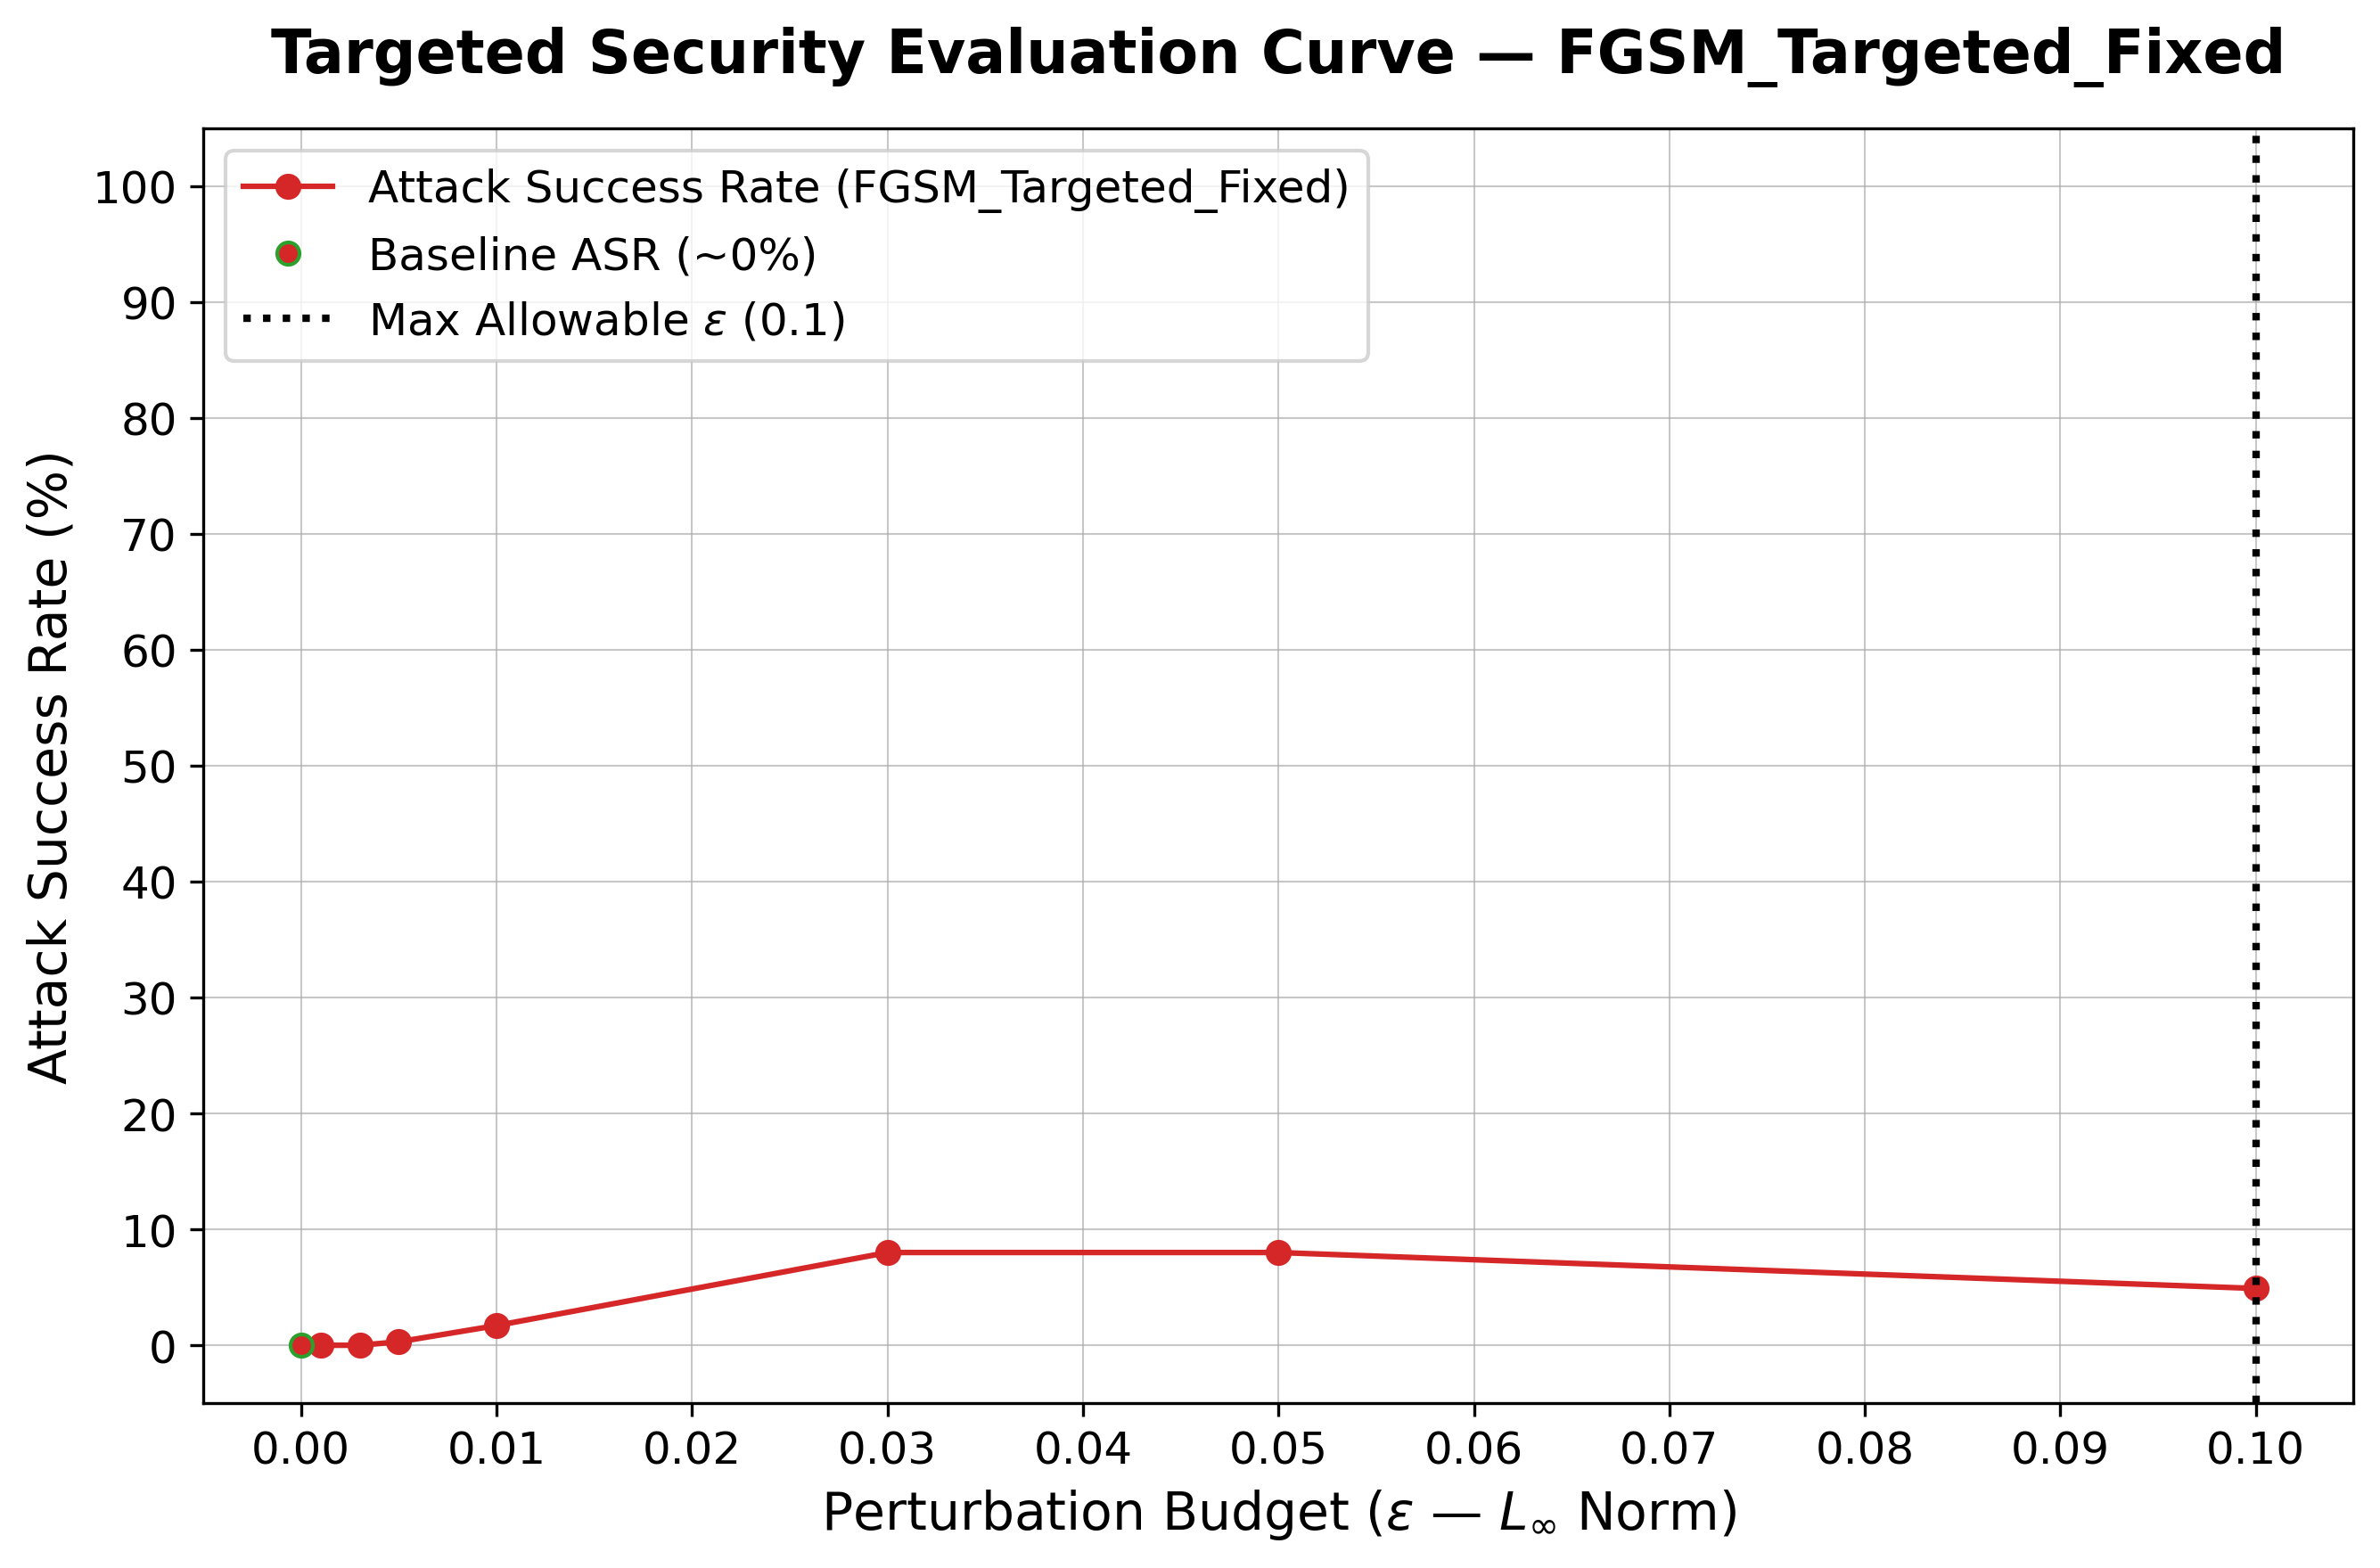
\includegraphics[width=1\linewidth]{FGSM_targeted/FGSM_Targeted_Fixed_SEC.png}
    \caption{Fixed FGSM SEC}
    \label{fig:targeted_FGSM_SEC}
\end{figure}

\begin{table}[H]
    \centering
    \begin{tabular}{ccccc}
        \toprule
        \textbf{$\epsilon$} & \textbf{Successful Attacks} & \textbf{Total Images} & \textbf{ASR (\%)} & \textbf{Time (s)} \\
        \midrule
        0.001 & 0  & 1000 & 0.0 & 16.43 \\
        0.003 & 0  & 1000 & 0.0 & 16.02 \\
        0.005 & 3  & 1000 & 0.3 & 15.32 \\
        0.01  & 17 & 1000 & 1.7 & 14.18 \\
        0.03  & 80 & 1000 & 8.0 & 14.07 \\
        0.05  & 80 & 1000 & 8.0 & 13.59 \\
        0.1   & 49 & 1000 & 4.9 & 13.95 \\
        \bottomrule
    \end{tabular}
    \caption{Valutazione dell'attacco FGSM in modalità \textit{Fixed} al variare di $\epsilon$}
    \label{tab:FGSM_targeted_fixed}
\end{table}

\subsubsection*{Least Likely Attack}
La modalità \textit{Least Likely} rappresenta la sfida offensiva più estrema per un algoritmo di perturbazione. In questo scenario, l'attacco non mira a una classe predefinita fissa, bensì a quella che il modello originario reputa la meno probabile in assoluto per la specifica immagine in esame. Geometricamente, ciò equivale a forzare l'input ad attraversare tutte le classi per raggiungere la regione dello spazio decisionale più distante dalla \textit{ground truth}.

Analizzando la \textit{Targeted SEC} (figura~\ref{fig:FGSM_Targeted_LeastLikely_SEC} e i dati quantitativi estratti in tabella~\ref{tab:FGSM_targeted_least_likely} per questa variante, emerge in modo inequivocabile il fallimento quasi totale dell'algoritmo FGSM. Per l'intero spettro dei budget di perturbazione analizzati, l'\textit{Attack Success Rate} (ASR) si mantiene su percentuali prossime allo zero. Anche spingendo il rumore al limite massimo consentito dai test ($\epsilon = 0.1$), l'algoritmo si dimostra incapace di guidare l'immagine verso la specifica etichetta bersaglio con un tasso di successo rilevante.

La spiegazione di questo fenomeno risiede nei limiti matematici intrinseci della natura \textit{single-step} del \textit{Fast Gradient Sign Method}. FGSM calcola un'unica direzione di massima pendenza verso il bersaglio e applica un singolo, massiccio sbalzo lungo quel vettore. Tuttavia, i confini decisionali di reti neurali profonde come \textit{InceptionResnetV1} sono non lineari e lo spazio semantico di VGGFace2 è estremamente denso (8631 classi). 

Tentare di coprire una distanza così ampia con un movimento rettilineo e in un solo passaggio fa sì che l'immagine vettoriale "attraversi" inevitabilmente le regioni di competenza di innumerevoli altre classi intermedie. Di conseguenza, l'attacco riesce quasi sempre a distruggere la predizione originaria (agendo di fatto come un potente attacco \textit{error-generic}), ma finisce una classe sbagliata, fallendo sistematicamente l'inganno mirato verso la destinazione \textit{Least Likely}.

Questi risultati empirici dimostrano in modo inconfutabile che gli approcci \textit{single-step} sono strutturalmente inadeguati per le alterazioni mirate complesse. Per forzare il modello verso bersagli così remoti.

\begin{figure}[h]
    \centering
    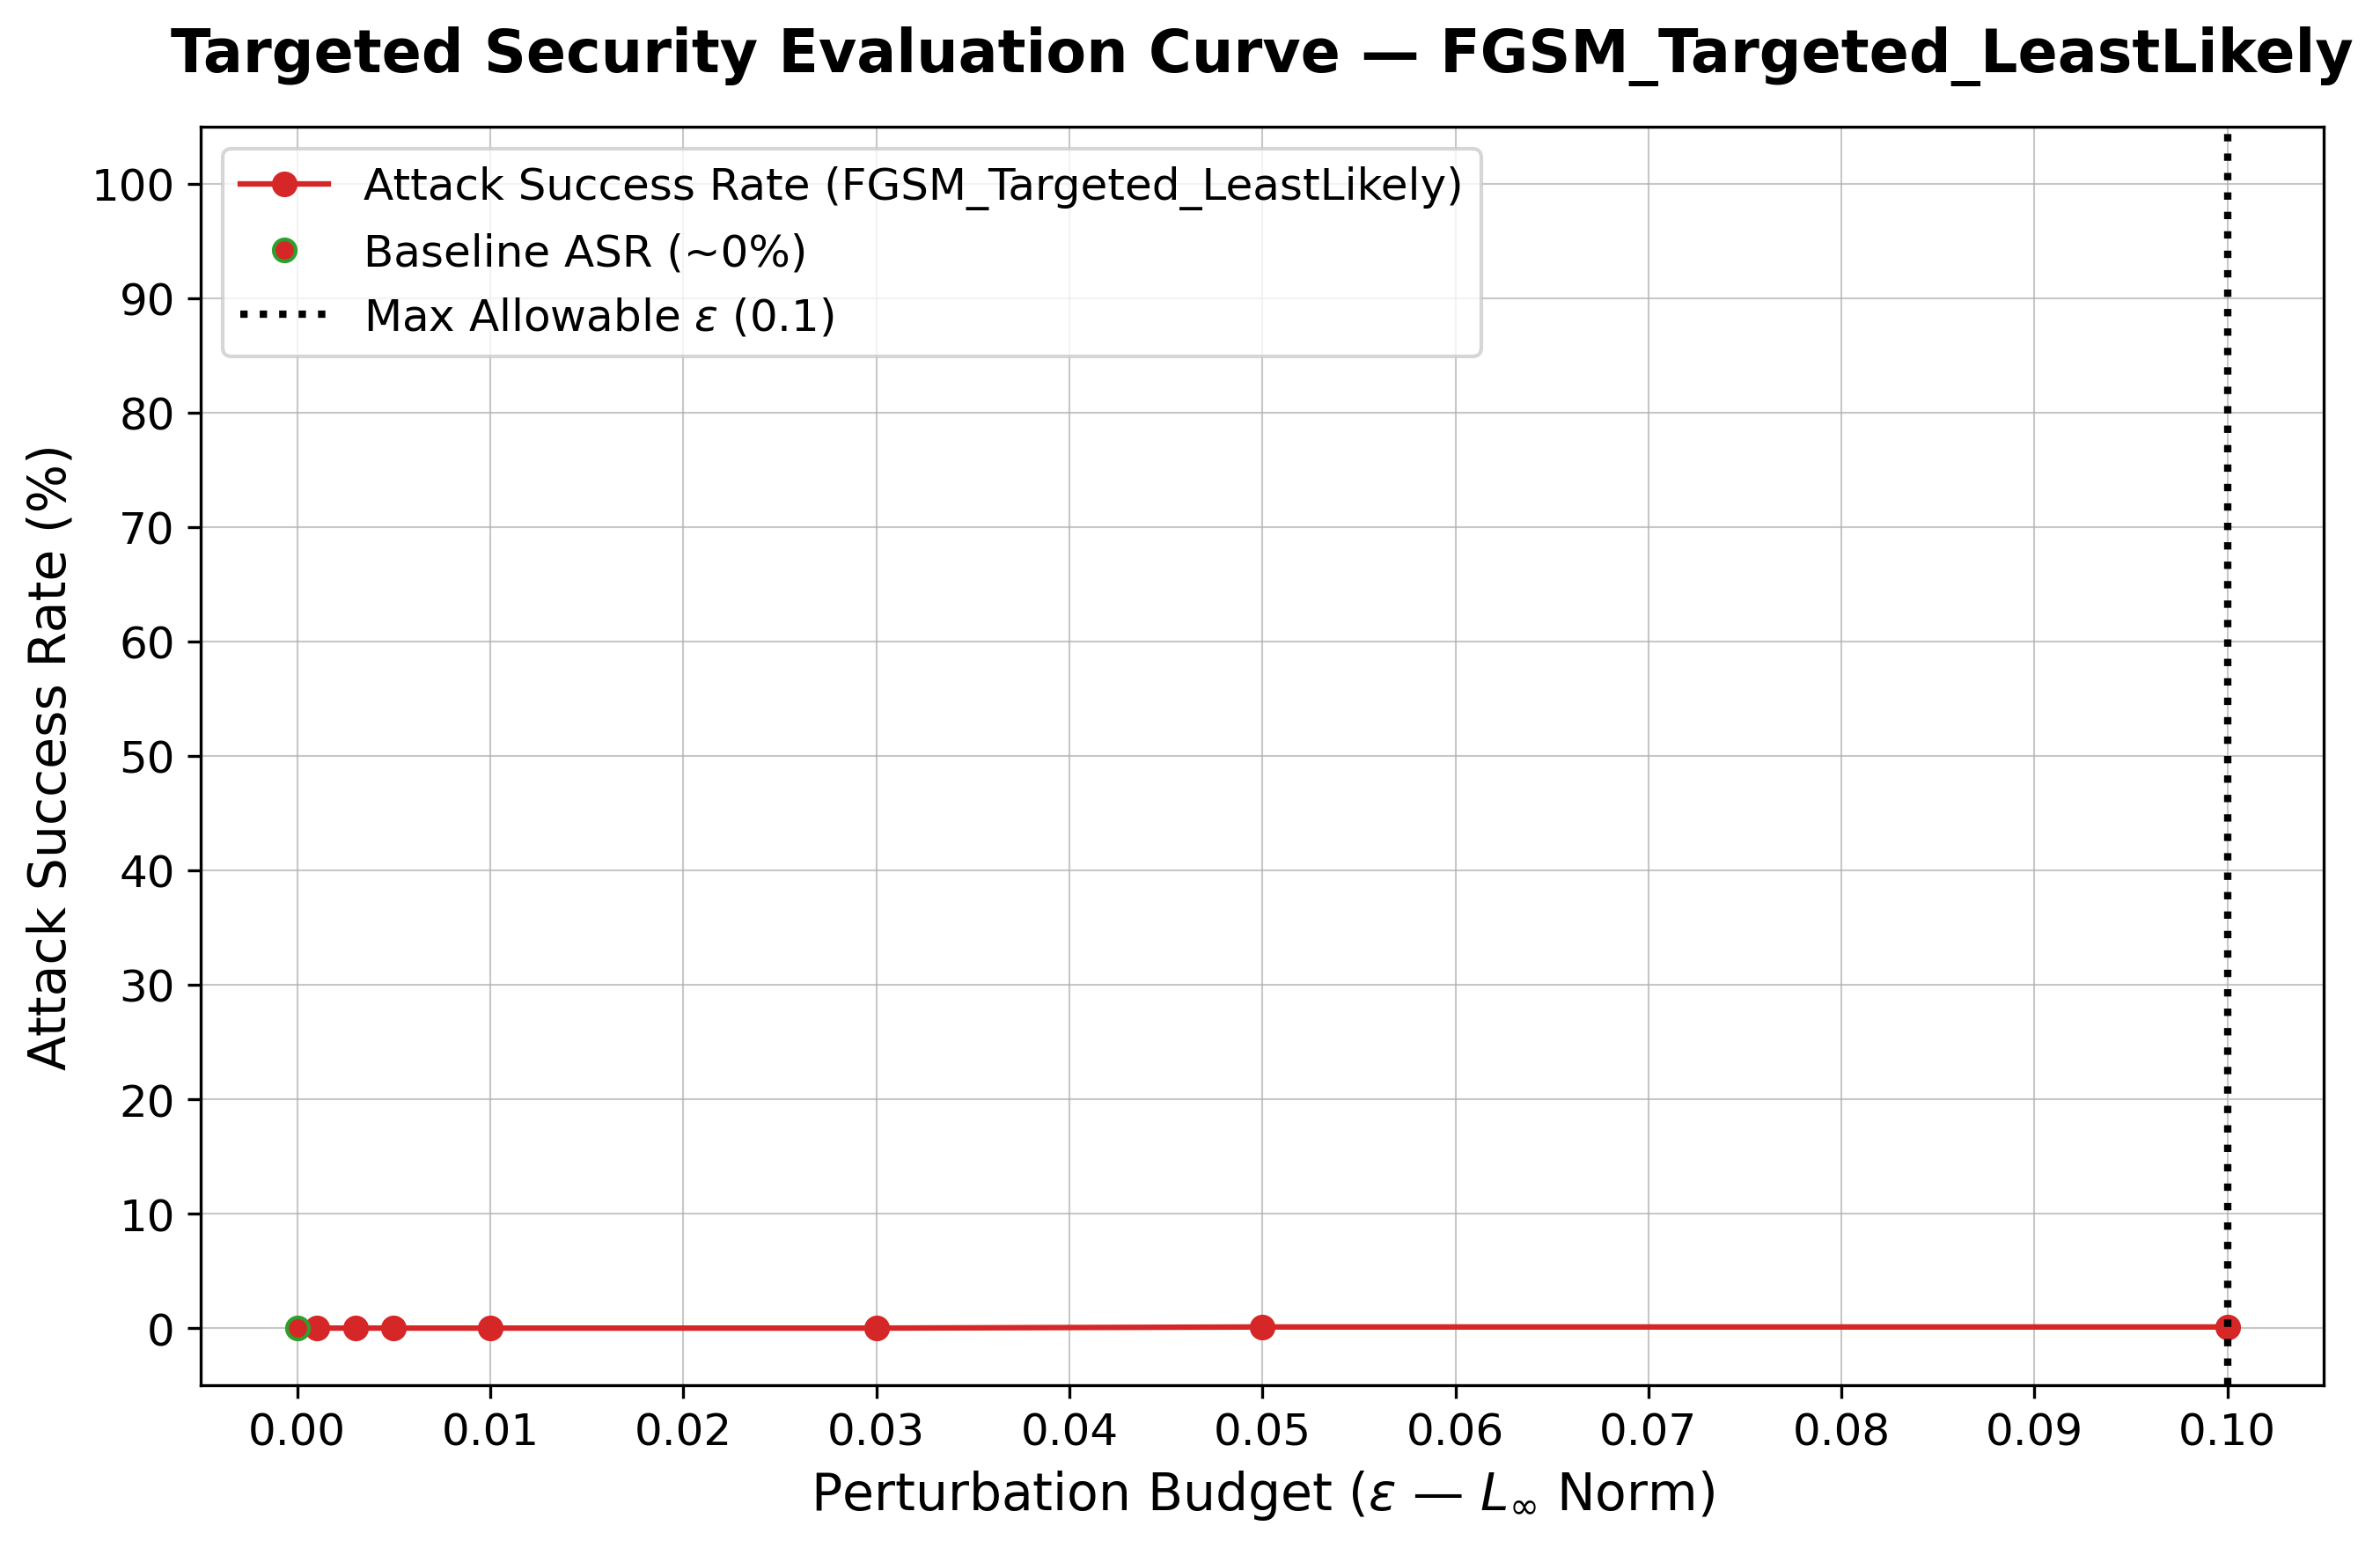
\includegraphics[width=1\linewidth]{FGSM_targeted/FGSM_Targeted_LeastLikely_SEC.png}
    \caption{Least Likley FGSM SEC}
    \label{fig:FGSM_Targeted_LeastLikely_SEC}
\end{figure}

\begin{table}[H]
    \centering
    \begin{tabular}{ccccc}
        \toprule
        \textbf{$\epsilon$} & \textbf{Successful Attacks} & \textbf{Total Images} & \textbf{ASR (\%)} & \textbf{Time (s)} \\
        \midrule
        0.001 & 0  & 1000 & 0.0 & 16.26 \\
        0.003 & 0  & 1000 & 0.0 & 15.83 \\
        0.005 & 0  & 1000 & 0.0 & 15.31 \\
        0.01  & 0  & 1000 & 0.0 & 14.11 \\
        0.03  & 0  & 1000 & 0.0 & 14.23 \\
        0.05  & 1  & 1000 & 0.1 & 13.49 \\
        0.1   & 1  & 1000 & 0.1 & 13.79 \\
        \bottomrule
    \end{tabular}
    \caption{Valutazione dell'attacco FGSM in modalità \textit{Least Likely} al variare di $\epsilon$}
    \label{tab:FGSM_targeted_least_likely}
\end{table}

\clearpage
\subsubsection{Basic Iterative Method (BIM)}
Come dimostrato dall'analisi della variante \textit{single-step} (FGSM), gli attacchi mirati in spazi decisionali complessi richiedono una precisione che un singolo sbalzo perturbativo non può garantire. Il \textit{Basic Iterative Method} (BIM) interviene esattamente per sanare questa criticità.

L'obiettivo algoritmico rimane la minimizzazione della \textit{loss} rispetto a una classe predeterminata ($y_{target}$). Tuttavia, invece di applicare l'intero \textit{budget} $\epsilon$ in un'unica soluzione, BIM suddivide la perturbazione in step frazionari di ampiezza ridotta ($\alpha = \epsilon / \text{max\_iter}$), ricalcolando il gradiente ad ogni iterazione. Questa strategia permette all'attacco di tracciare un percorso che aggira i confini delle classi intermedie e guida progressivamente l'immagine verso la regione di pertinenza del bersaglio desiderato.

Formalmente, l'aggiornamento iterativo con proiezione si esprime come:
$$ x'_t = \Pi_\epsilon \left( x_{t-1} - \alpha \cdot \text{sign}(\nabla_x \mathcal{L}(h(x_{t-1}, w), y_{target})) \right) $$

Per valutare il tasso di successo (ASR) di questo approccio, la rete NN1 è stata sottoposta a test esplorando una matrice bidimensionale di parametri: il \textit{budget} di perturbazione e la profondità computazionale.

\begin{verbatim}
EPSILONS = [0.001, 0.003, 0.005, 0.01, 0.03, 0.05, 0.1]
MAX_ITER_LIST = [1, 5, 10, 20]

\end{verbatim}

Le sezioni seguenti presentano l'analisi quantitativa dei risultati, esplorando l'impatto del partizionamento dell'errore (iterazioni) sulla reale capacità di forzare un inganno mirato. Al fine di non appesantire ulteriormente la lettura dell'elaborato, è possibile consultare i valori precisi dei risultati empirici ottenuti durante la fase di test, alle seguenti cartelle:
\begin{itemize}
    \item \href{https://github.com/ChristianRosa02/AI4Cybersecurity/blob/master/results/BIM_Targeted_Fixed/BIM_Targeted_Fixed_results.csv}{risultati fixed}
    \item \href{https://github.com/ChristianRosa02/AI4Cybersecurity/blob/master/results/BIM_Targeted_LeastLikely/BIM_Targeted_LeastLikely_results.csv}{risultati Least Likely}
\end{itemize}

\clearpage
\subsubsection*{Fixed Attack}
L'analisi della modalità \textit{Fixed} per l'attacco BIM rivela in modo lampante la superiorità geometrica dell'approccio iterativo nel risolvere il complesso problema dell'inganno mirato. Confrontando i risultati con quelli ottenuti nella medesima configurazione tramite FGSM, emerge un divario prestazionale sostanziale, interamente imputabile al partizionamento del \textit{budget} di perturbazione.

Osservando la curva comparativa delle \textit{Targeted SEC}, la configurazione con \texttt{max\_iter} = 1 (matematicamente equivalente a un attacco FGSM) conferma il fallimento dell'approccio \textit{single-step}: l'\textit{Attack Success Rate} (ASR) rimane piatto e marginale lungo l'intero asse delle ascisse, dimostrando l'incapacità di raggiungere il bersaglio prefissato (la classe 2026).

Tuttavia, non appena il \textit{budget} viene suddiviso in step successivi, le performance offensive subiscono un aumento significativo. Aumentando il numero di iterazioni da 1 a 5, l'ASR inizia a crescere significativamente per valori di $\epsilon > 0.03$.

Il vero collasso delle difese del modello si registra spingendo l'algoritmo verso le 10 e le 20 iterazioni. Con \texttt{max\_iter} = 20 e un budget \textit{high-level} ($\epsilon = 0.1$), l'attacco riesce a forzare con successo il furto d'identità in un'altissima percentuale dei casi. Questo dimostra che, se guidato attraverso piccoli passi correttivi sequenziali (ricalcolando la pendenza della \textit{loss} ad ogni step), il rumore limitato entro la norma $L_\infty$ è perfettamente in grado di aggirare gli ostacoli dimensionali e finire nella regione di pertinenza del target.

Il grafico relativo all'effetto degli iperparametri (\textit{max\_iter effect}) evidenzia inoltre una chiara dinamica di saturazione. La transizione tra 1 e 10 iterazioni garantisce guadagni in ASR pressoché verticali. Tuttavia, il passaggio da 10 a 20 iterazioni produce un incremento marginale nettamente inferiore, confermando che l'algoritmo tende a convergere verso il suo massimo potenziale attorno al decimo step. Oltre questa soglia, un ulteriore frazionamento del gradiente non è giustificato da un proporzionale aumento dell'efficacia.

In figura~\ref{fig:BIM_Targeted_Fixed_comparative_SEC} è possibile vedere l'effetto di ogni singolo valore per \texttt{max\_iter}. Inoltre, una vista più dettagliata è offeta nella matrice di immagini in figura~\ref{fig:matrice_iterazioni_fixed_BIM}

\begin{figure}[h]
    \centering
    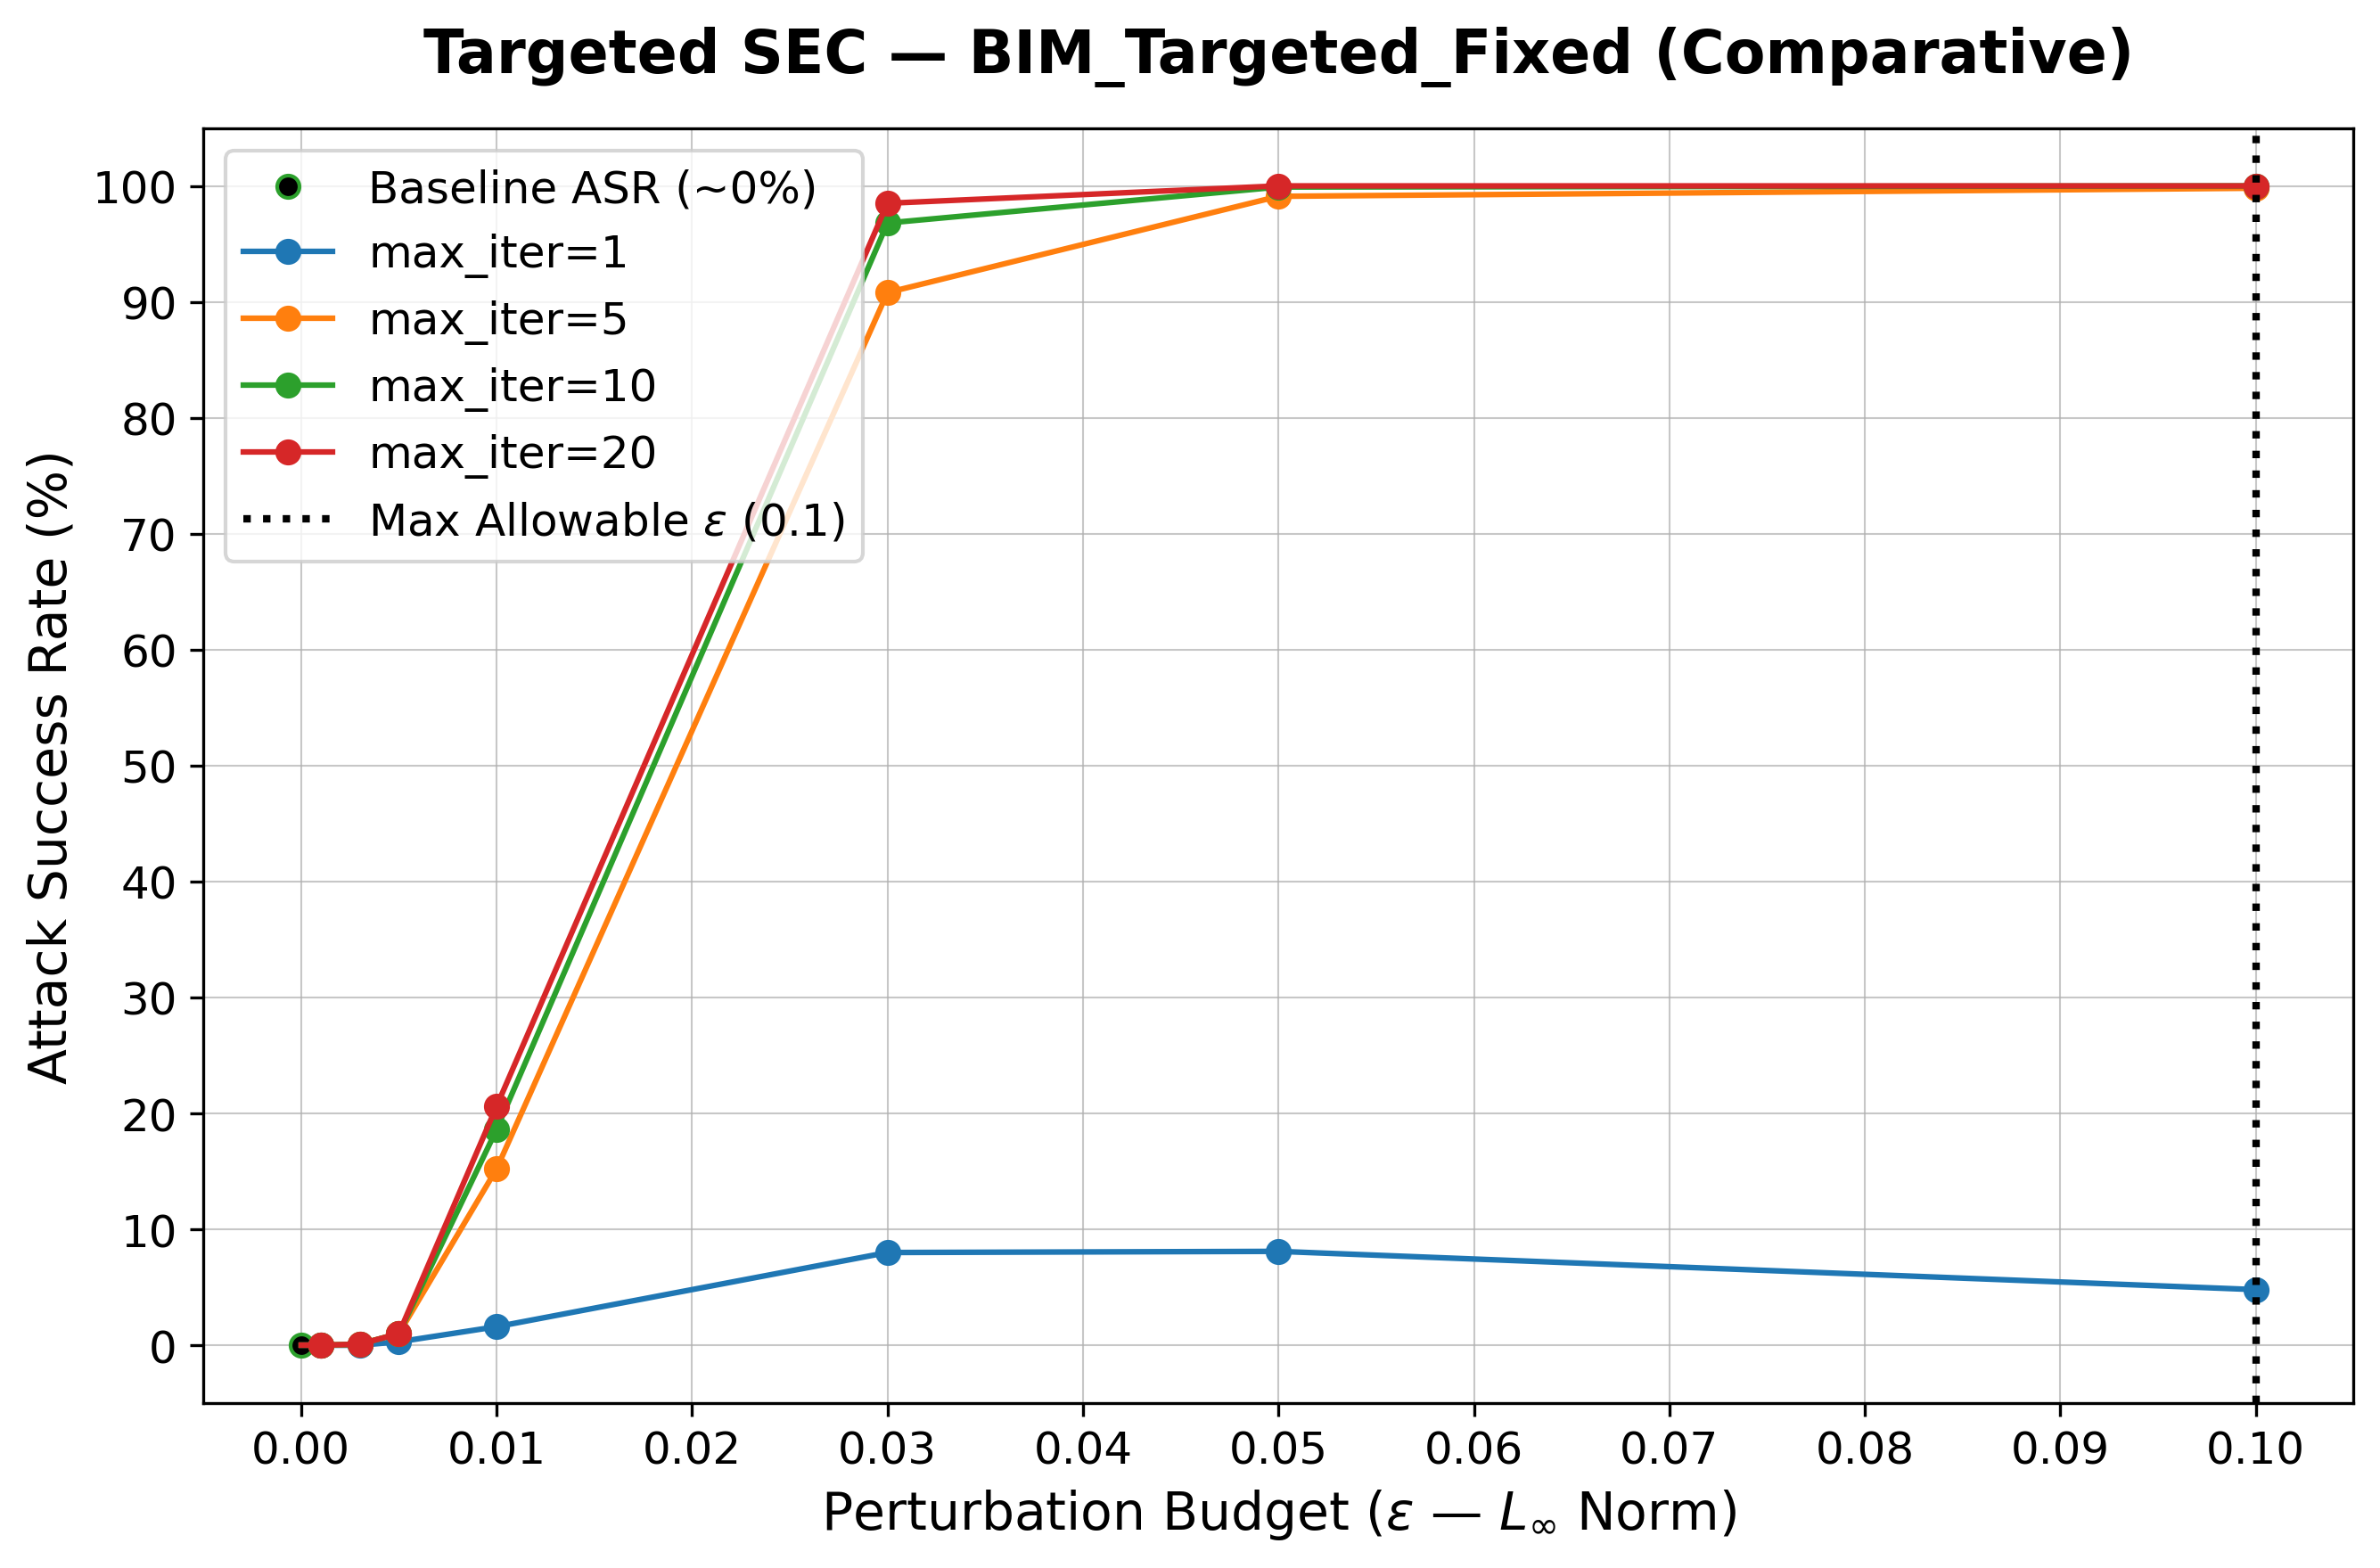
\includegraphics[width=0.8\linewidth]{BIM_Error_specific/fixed/BIM_Targeted_Fixed_comparative_SEC.png}
    \caption{BIM Fixed SEC}
    \label{fig:BIM_Targeted_Fixed_comparative_SEC}
\end{figure}

\begin{figure}[H]
    \centering
    % Inizio del trucco per far uscire le immagini dai margini
    \makebox[\textwidth][c]{
        \begin{tabular}{cc} % Usiamo una tabella invisibile per tenere la struttura ferma
            
            % Prima subfigure (sinistra, riga 1)
            \begin{subfigure}[b]{0.55\textwidth}
                \centering
                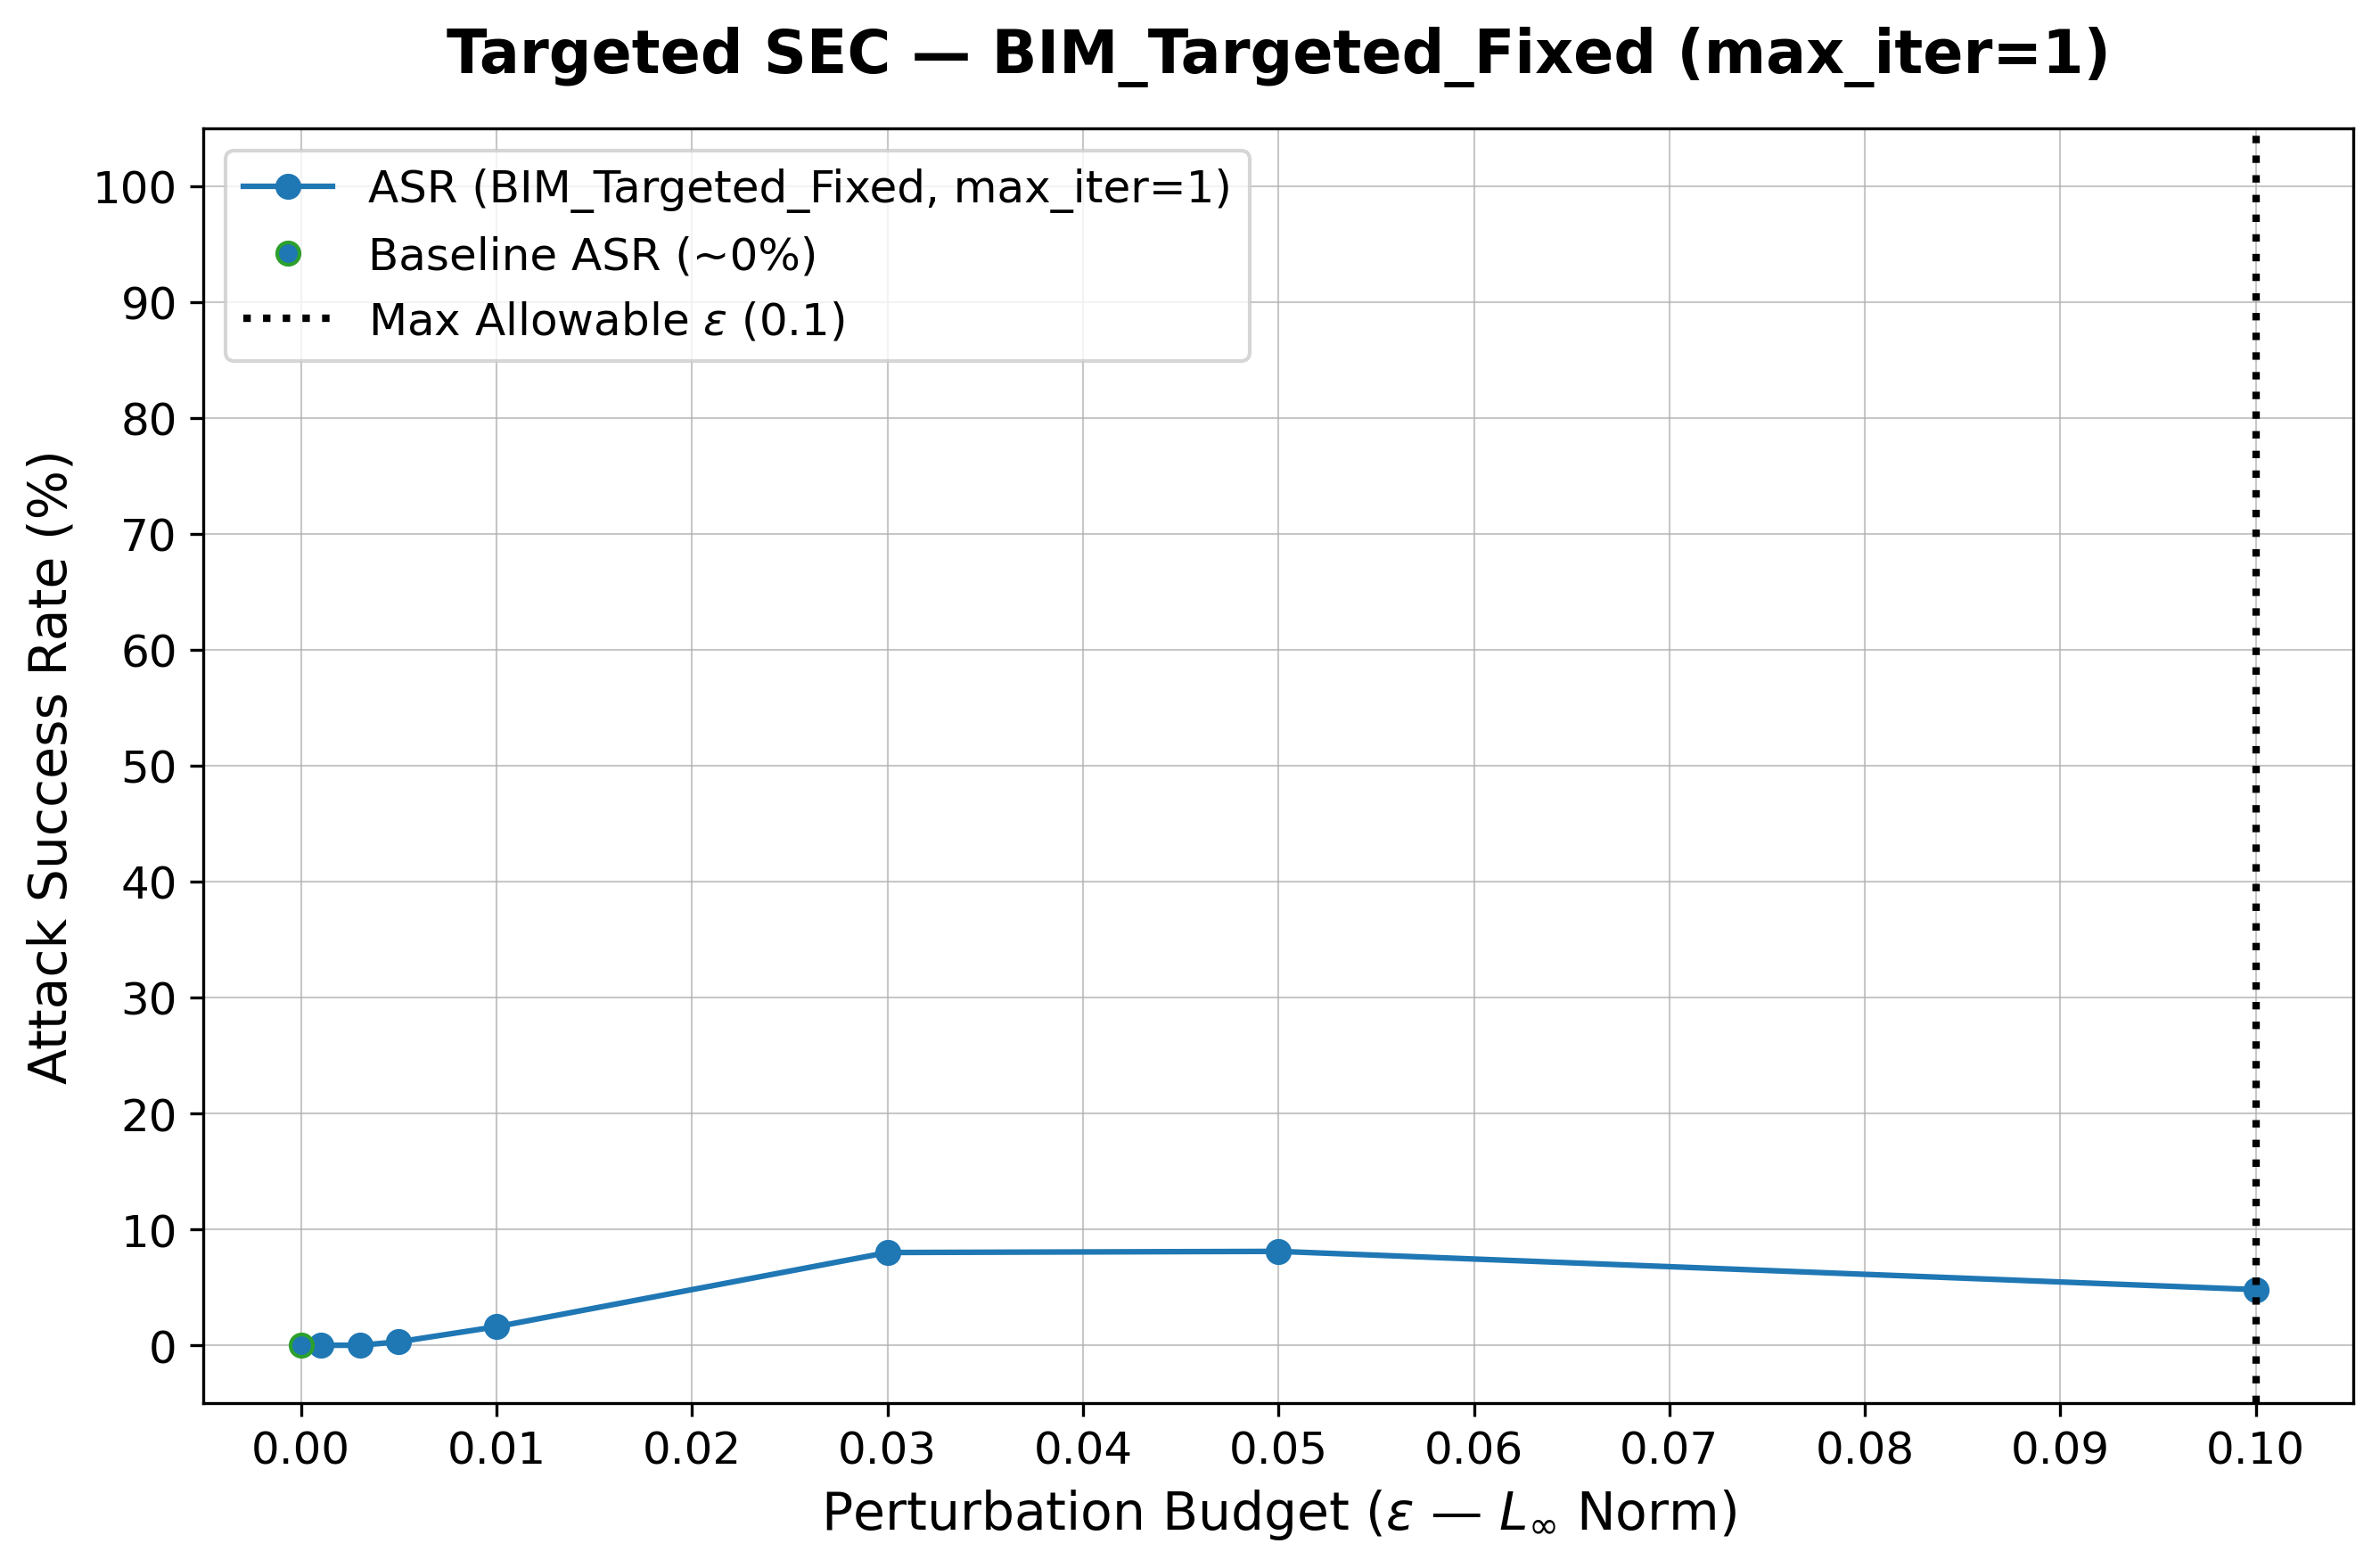
\includegraphics[width=\textwidth]{BIM_Error_specific/fixed/BIM_Targeted_Fixed_iter1_SEC.png}
                \caption{Iterazione 1}
                \label{fig:iter1}
            \end{subfigure} 
            & 
            % Seconda subfigure (destra, riga 1)
            \begin{subfigure}[b]{0.55\textwidth}
                \centering
                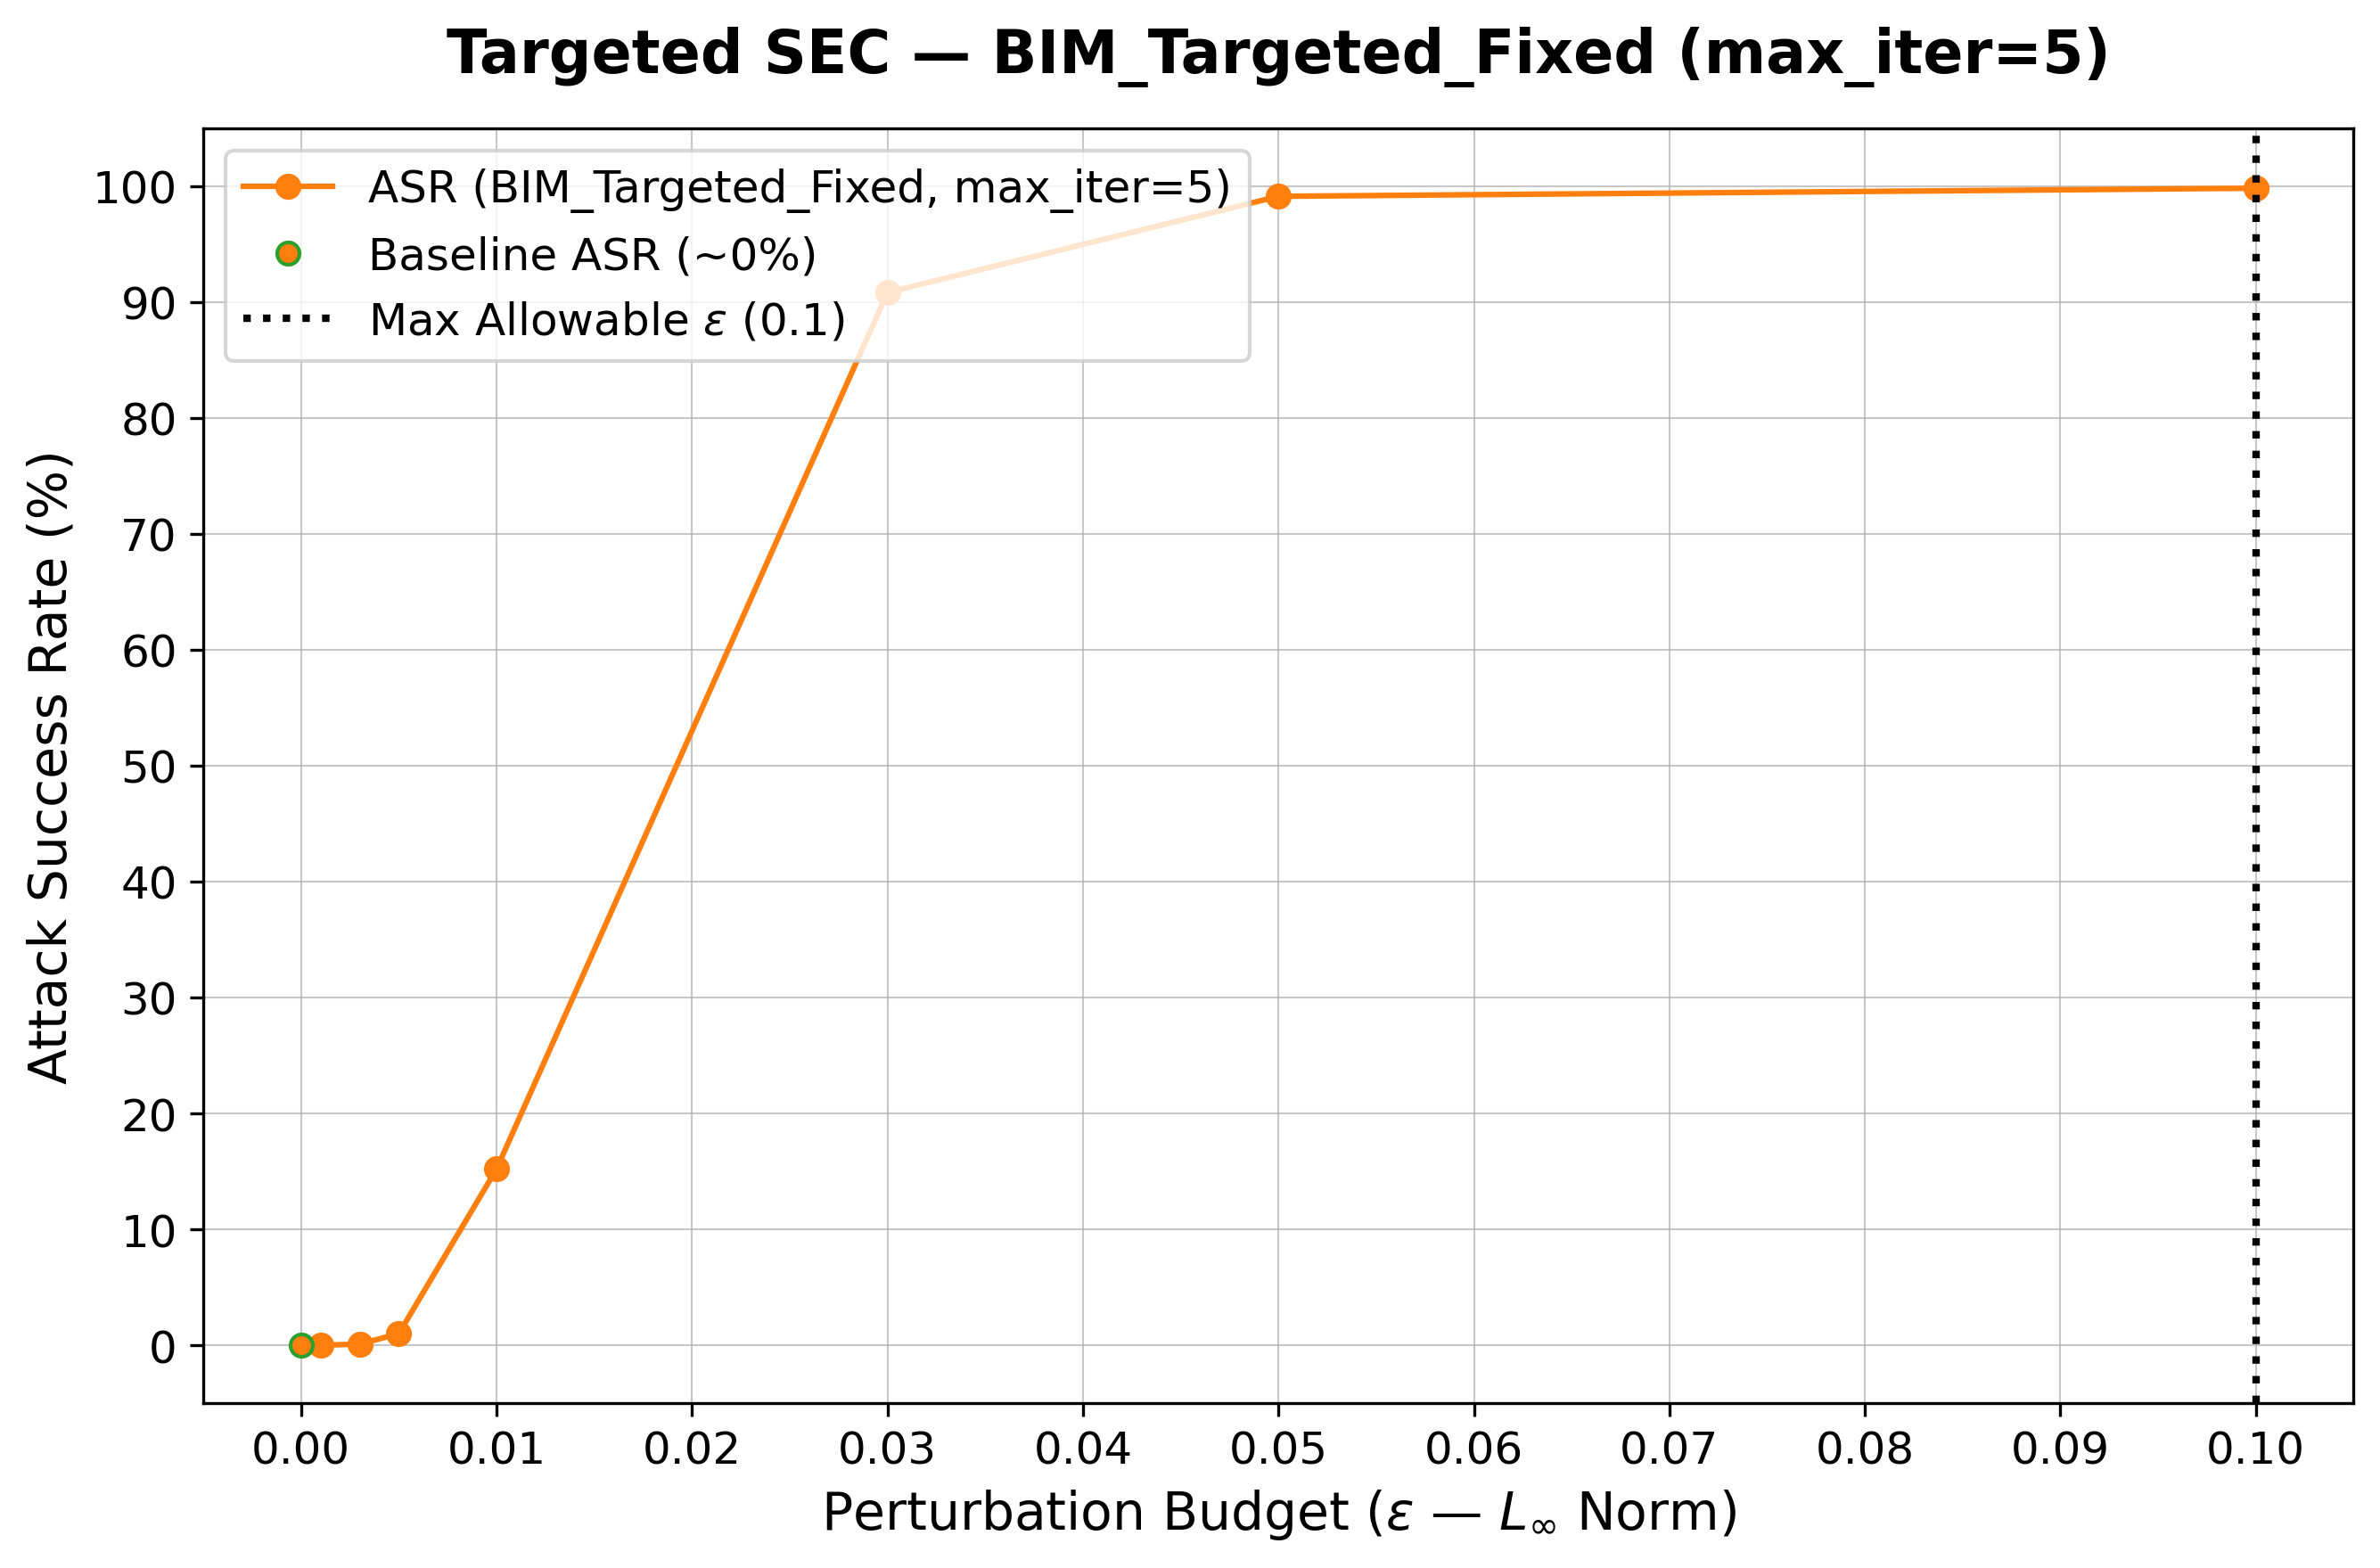
\includegraphics[width=\textwidth]{BIM_Error_specific/fixed/BIM_Targeted_Fixed_iter5_SEC.png}
                \caption{Iterazione 5}
                \label{fig:iter5}
            \end{subfigure} \\ [0.5cm] % Spazio verticale tra le righe
            
            % Terza subfigure (sinistra, riga 2)
            \begin{subfigure}[b]{0.55\textwidth}
                \centering
                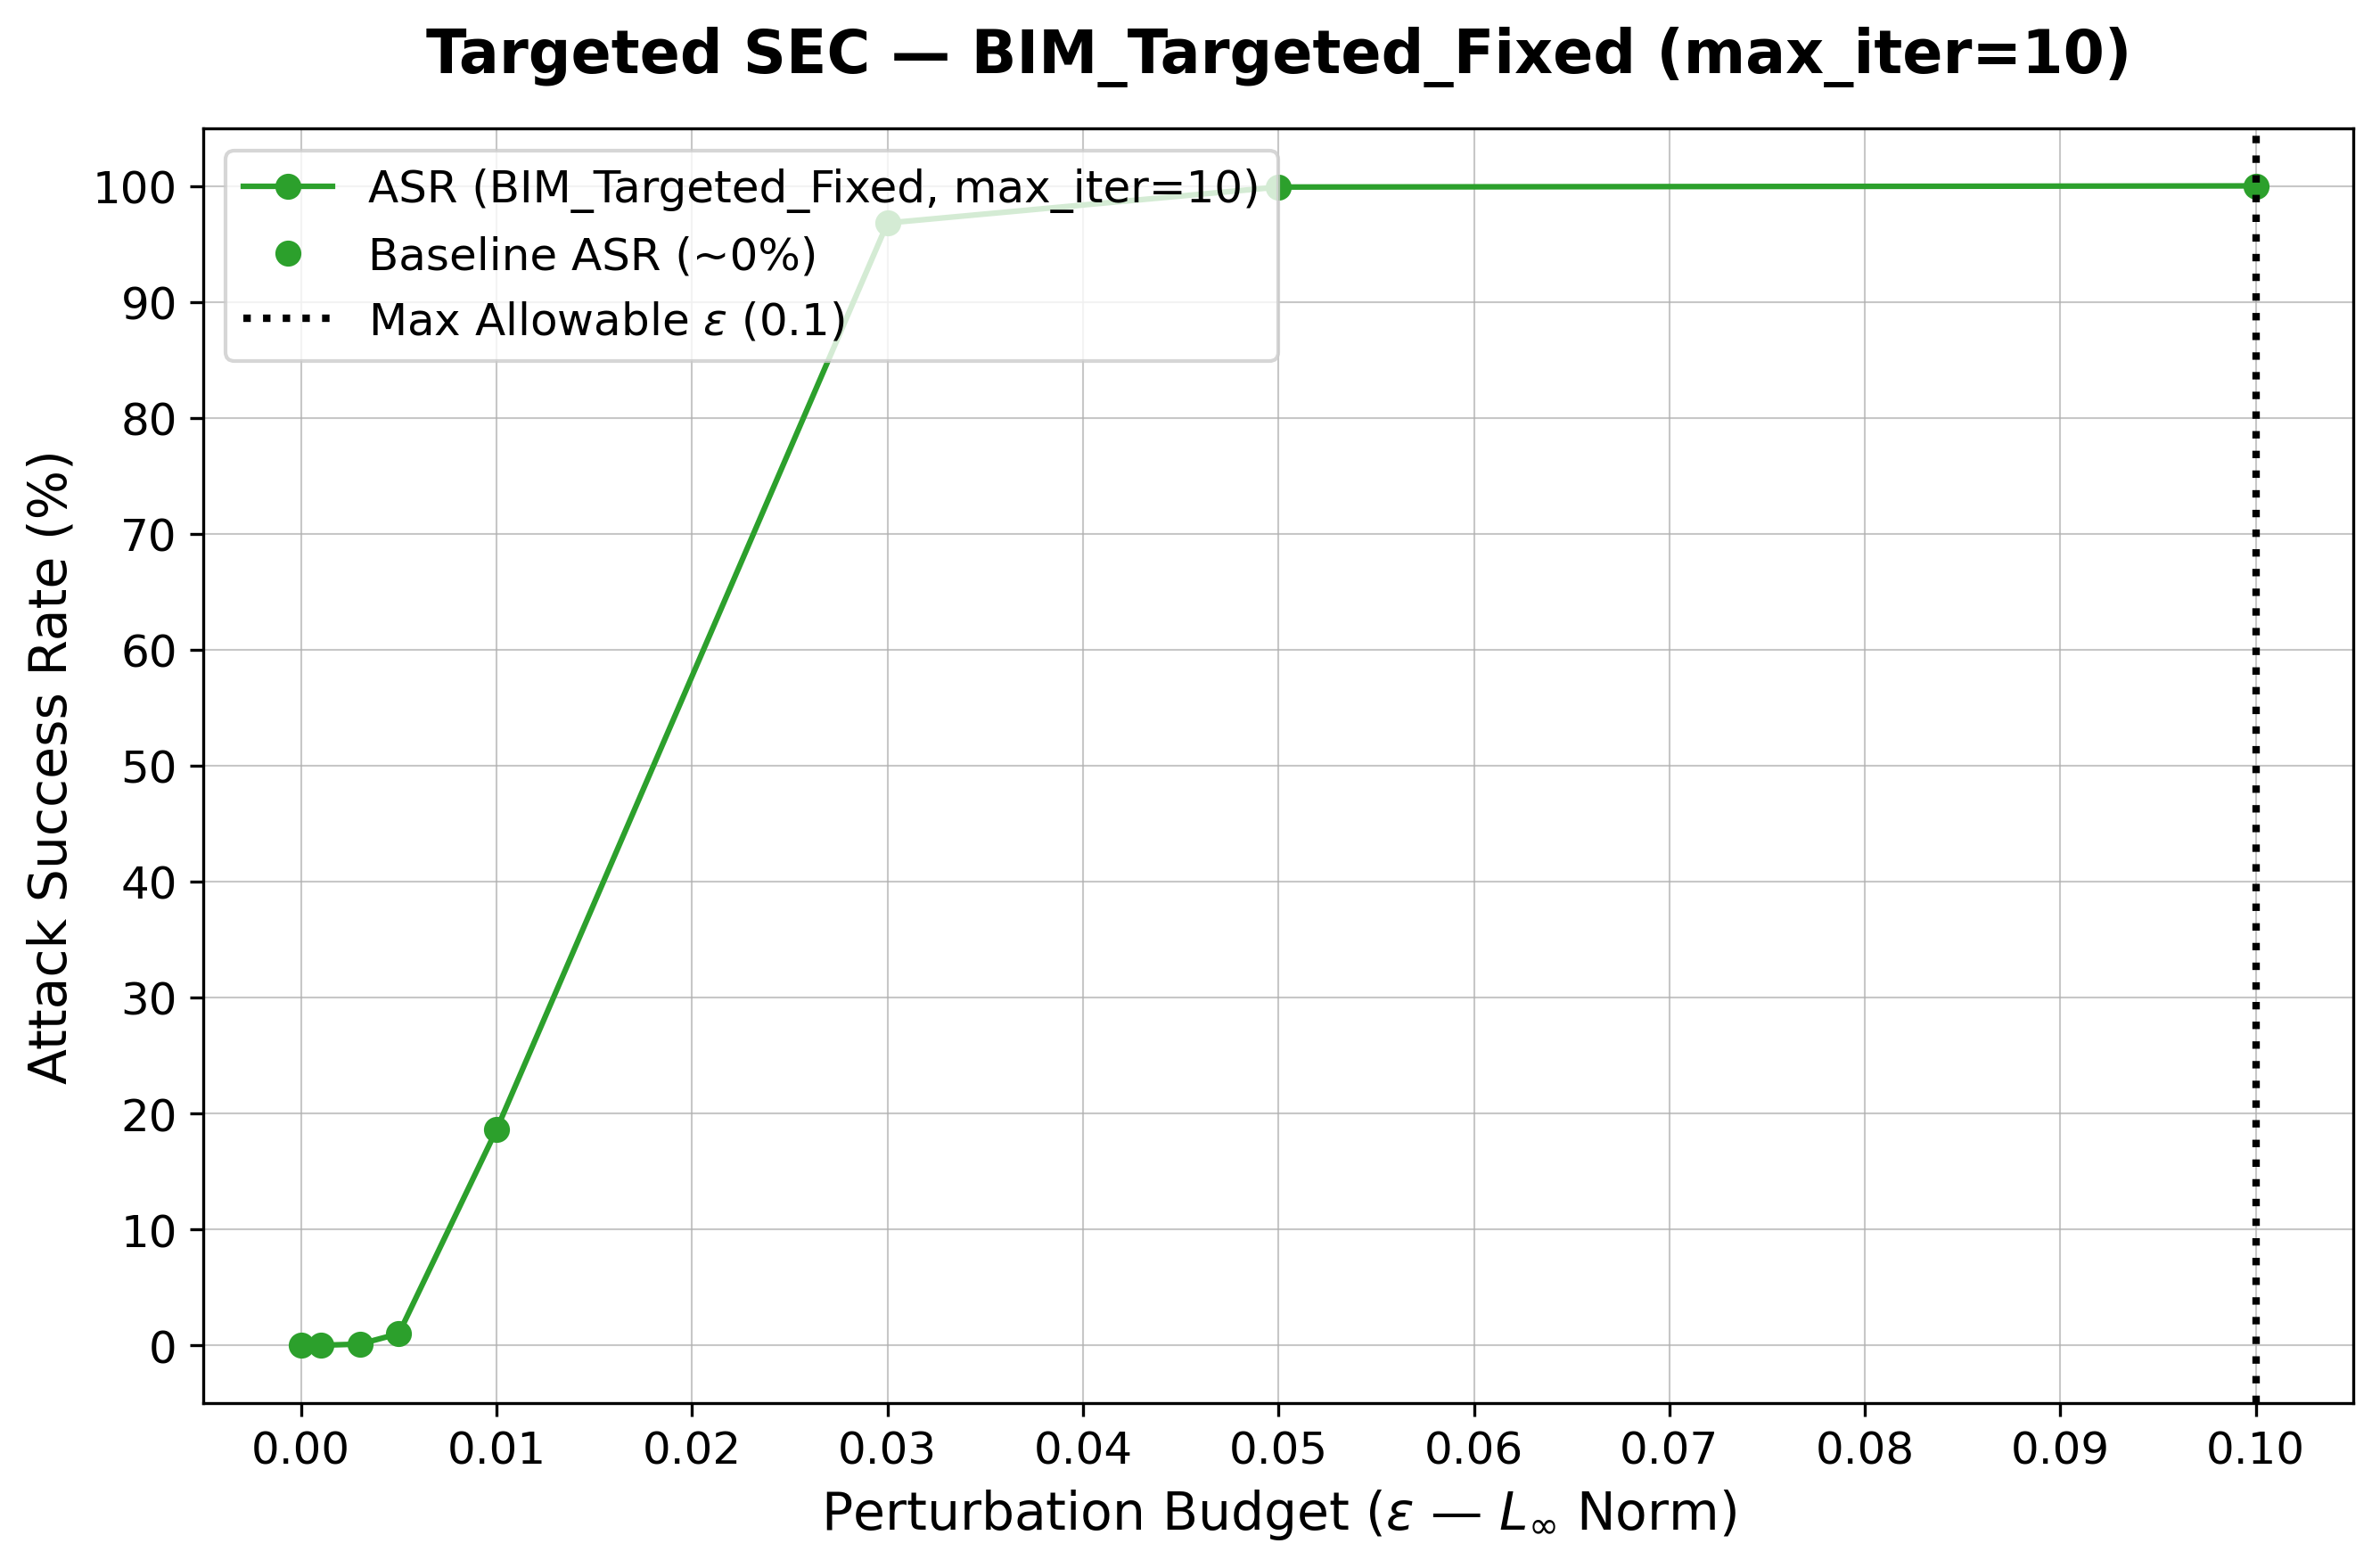
\includegraphics[width=\textwidth]{BIM_Error_specific/fixed/BIM_Targeted_Fixed_iter10_SEC.png}
                \caption{Iterazione 10}
                \label{fig:iter10}
            \end{subfigure} 
            & 
            % Quarta subfigure (destra, riga 2)
            \begin{subfigure}[b]{0.55\textwidth}
                \centering
                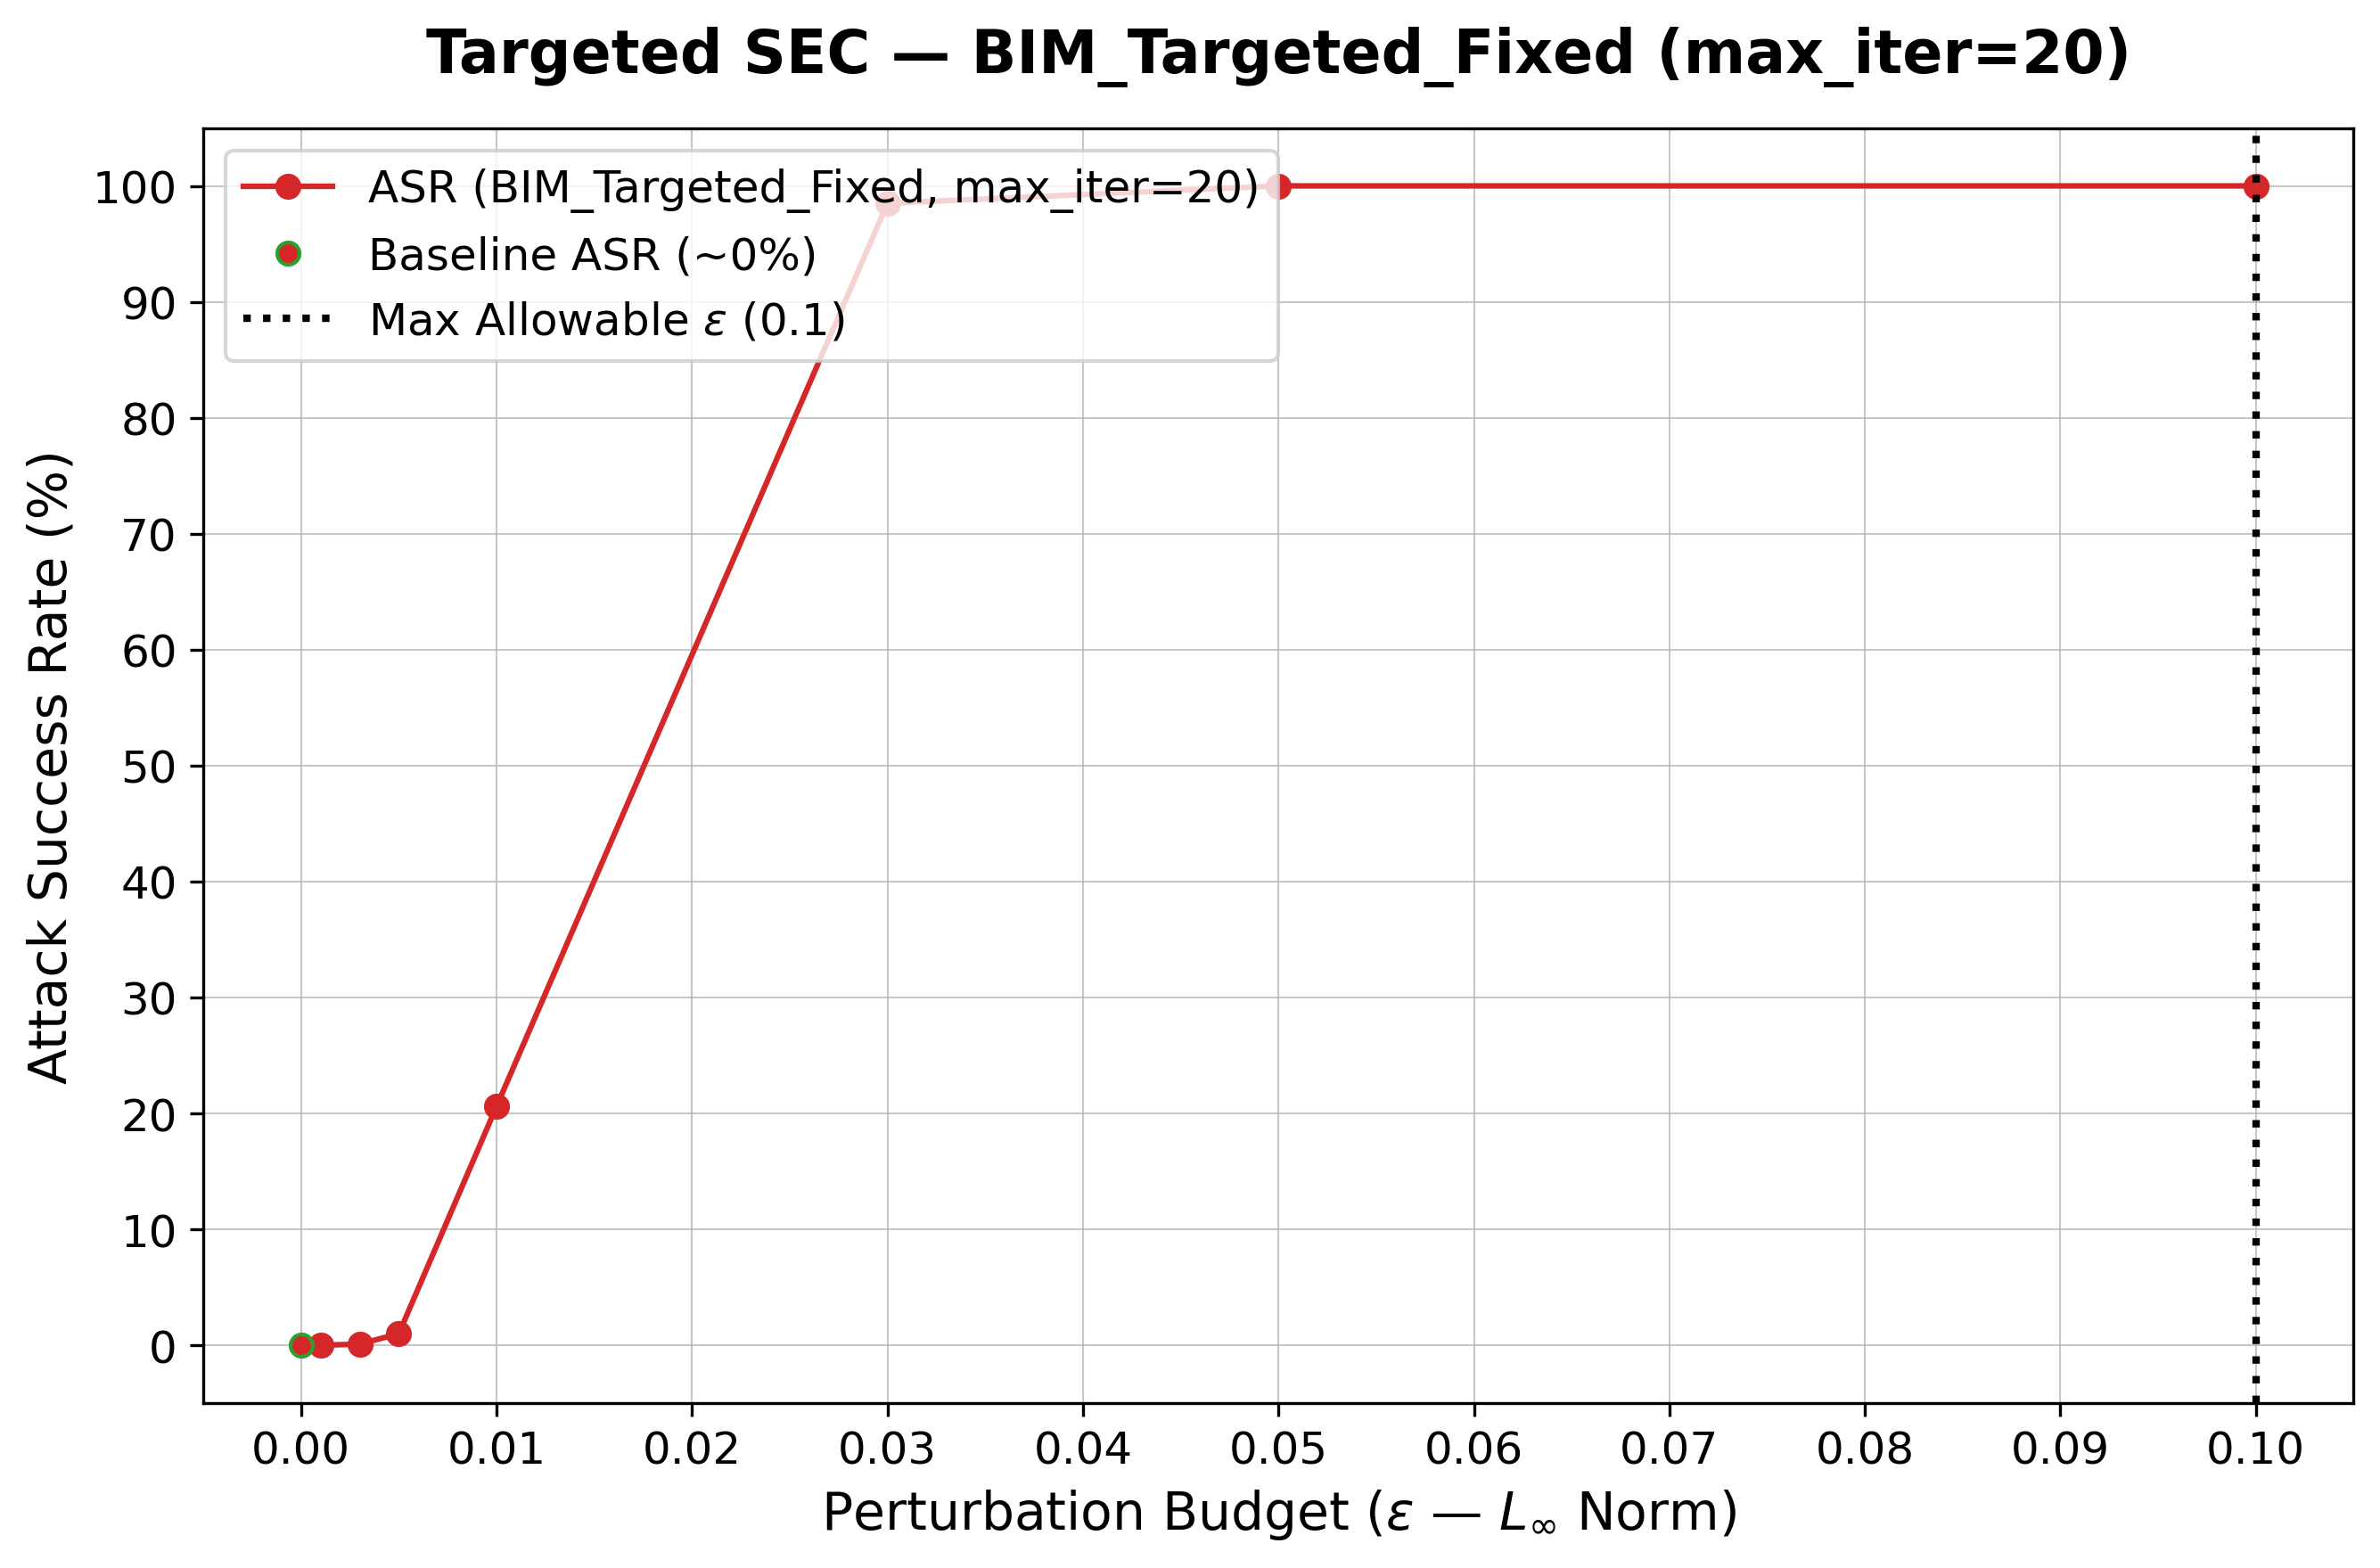
\includegraphics[width=\textwidth]{BIM_Error_specific/fixed/BIM_Targeted_Fixed_iter20_SEC.png}
                \caption{Iterazione 20}
                \label{fig:iter20}
            \end{subfigure}
            
        \end{tabular}
    } % Fine del \makebox
    
    \caption{Confronto dei risultati al variare delle iterazioni per fixed (1, 5, 10 e 20).}
    \label{fig:matrice_iterazioni_fixed_BIM}
\end{figure}

\clearpage
\subsubsection*{Least Likely Attack}
Coerentemente con i limiti teorici noti, la variante \textit{single-step} (\texttt{max\_iter} = 1) fallisce sistematicamente, confermando che un singolo vettore di perturbazione non può colmare distanze così ampie.

Il dato di maggior rilievo, tuttavia, emerge analizzando l'evoluzione dell'\textit{Attack Success Rate} (ASR) all'aumentare della profondità computazionale. Con un numero limitato di iterazioni (\texttt{max\_iter} = 5), l'attacco fatica ancora a raggiungere la regione di decisione opposta a quella della ground truth.
Il salto qualitativo avviene spingendo l'algoritmo verso le 10 e, soprattutto, le 20 iterazioni. Nella configurazione con \texttt{max\_iter} = 20 (curva rossa), non appena il \textit{budget} $\epsilon$ supera la soglia di 0.05, l'ASR subisce un aumento verticale non trascurabile. Al raggiungimento del limite massimo consentito ($\epsilon = 0.1$), il tasso di successo dell'attacco si attesta a valori prossimi al 100\%. 

Questo risultato empirico sfata l'assunzione che la distanza sia un ostacolo insormontabile per gli attacchi \textit{budget-constrained}. Dimostra in modo inconfutabile che, a patto di frazionare il gradiente in un numero sufficiente di micropassi, la perturbazione contenuta entro la norma $L_\infty$ possiede una flessibilità geometrica sufficiente per connettere qualsiasi punto dello spazio latente alla regione decisionale più distante. 

Il grafico relativo all'effetto del parametro iterativo (figura~\ref{fig:BIM_Targeted_LeastLikely_comparative_SEC}) dimostra questa dinamica: per la classe \textit{Least Likely}, la rete oppone una forte resistenza iniziale (curva blu) indipendentemente dal budget utilizzato. Il modello inizia a cedere quando all'algoritmo viene assegnato un numero di iterazioni elevato (20), confermando che i bersagli estremi richiedono un costo computazionale proporzionalmente superiore per garantire la riuscita dell'attacco. In figura~\ref{fig:matrice_iterazioni_LL_BIM} è fornita una vista dettagliata del grafico principale figura~\ref{fig:BIM_Targeted_LeastLikely_comparative_SEC}

\begin{figure}[h]
    \centering
    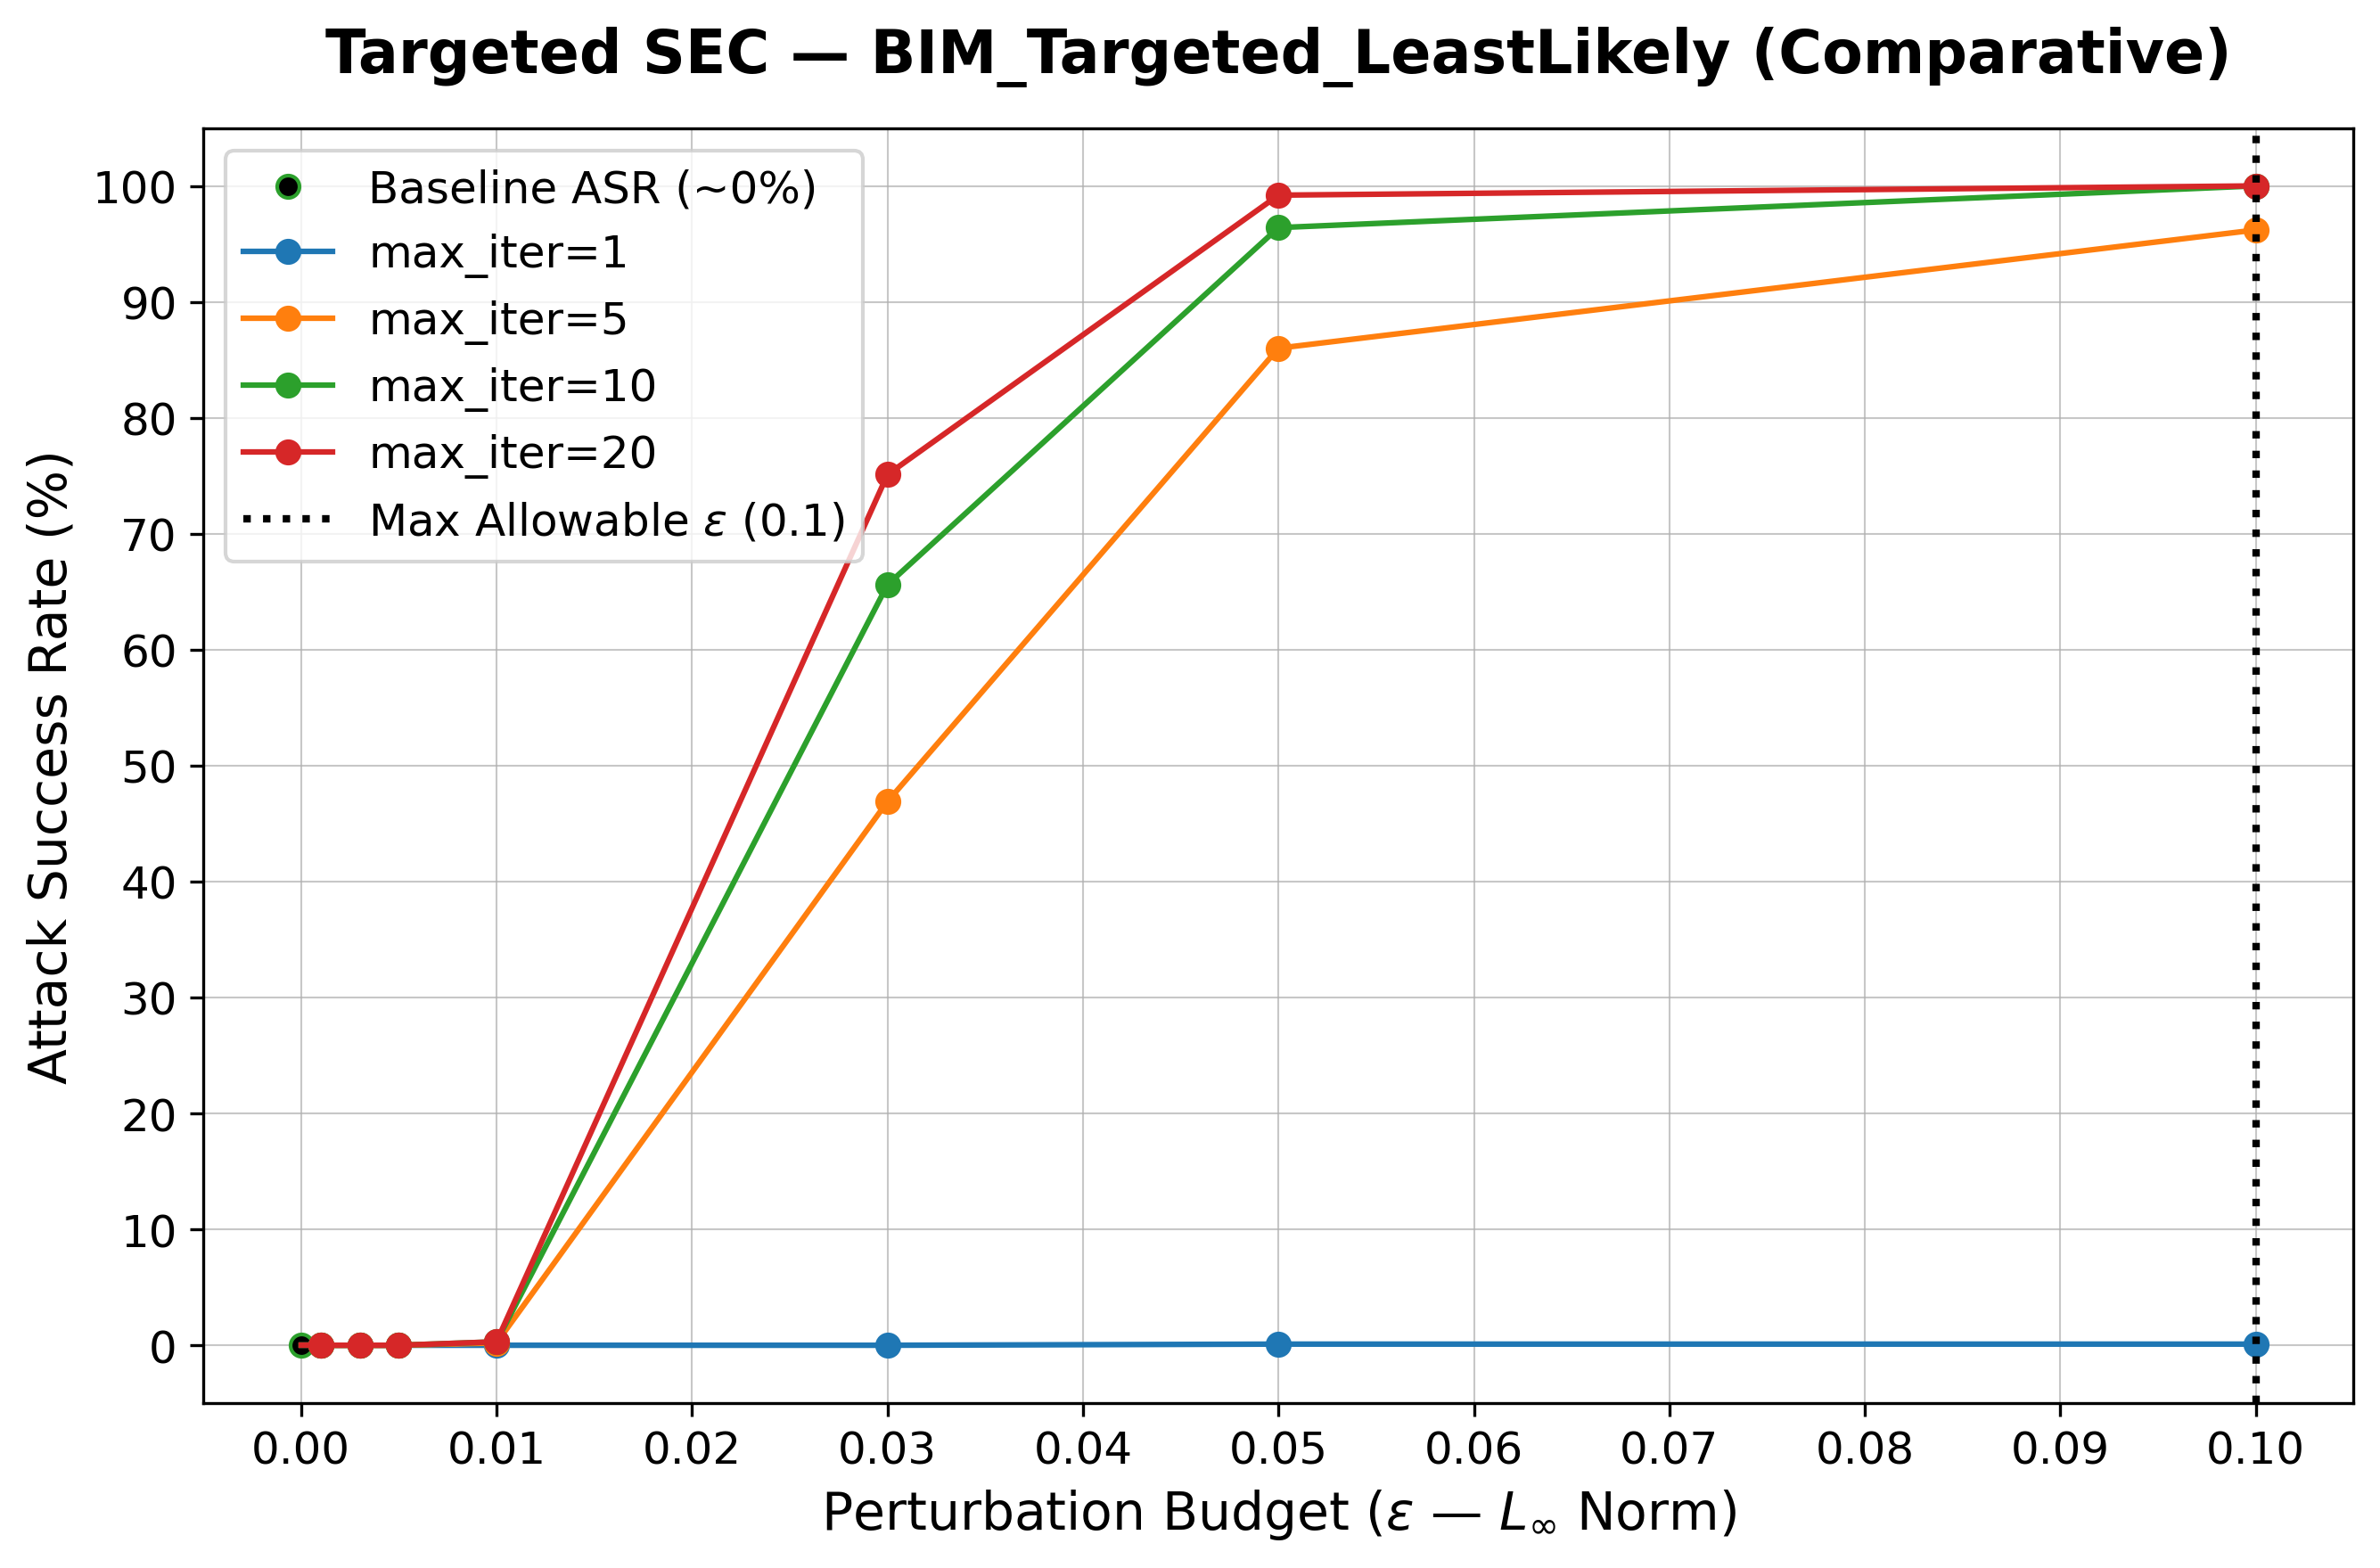
\includegraphics[width=1\linewidth]{BIM_Error_specific/LL/BIM_Targeted_LeastLikely_comparative_SEC.png}
    \caption{BIM LeastLikely SEC}
    \label{fig:BIM_Targeted_LeastLikely_comparative_SEC}
\end{figure}

\begin{figure}[H]
    \centering
    
    % Inizio del trucco per far uscire le immagini dai margini
    \makebox[\textwidth][c]{
        \begin{tabular}{cc}
            
            % Prima riga (sinistra)
            \begin{subfigure}[b]{0.55\textwidth}
                \centering
                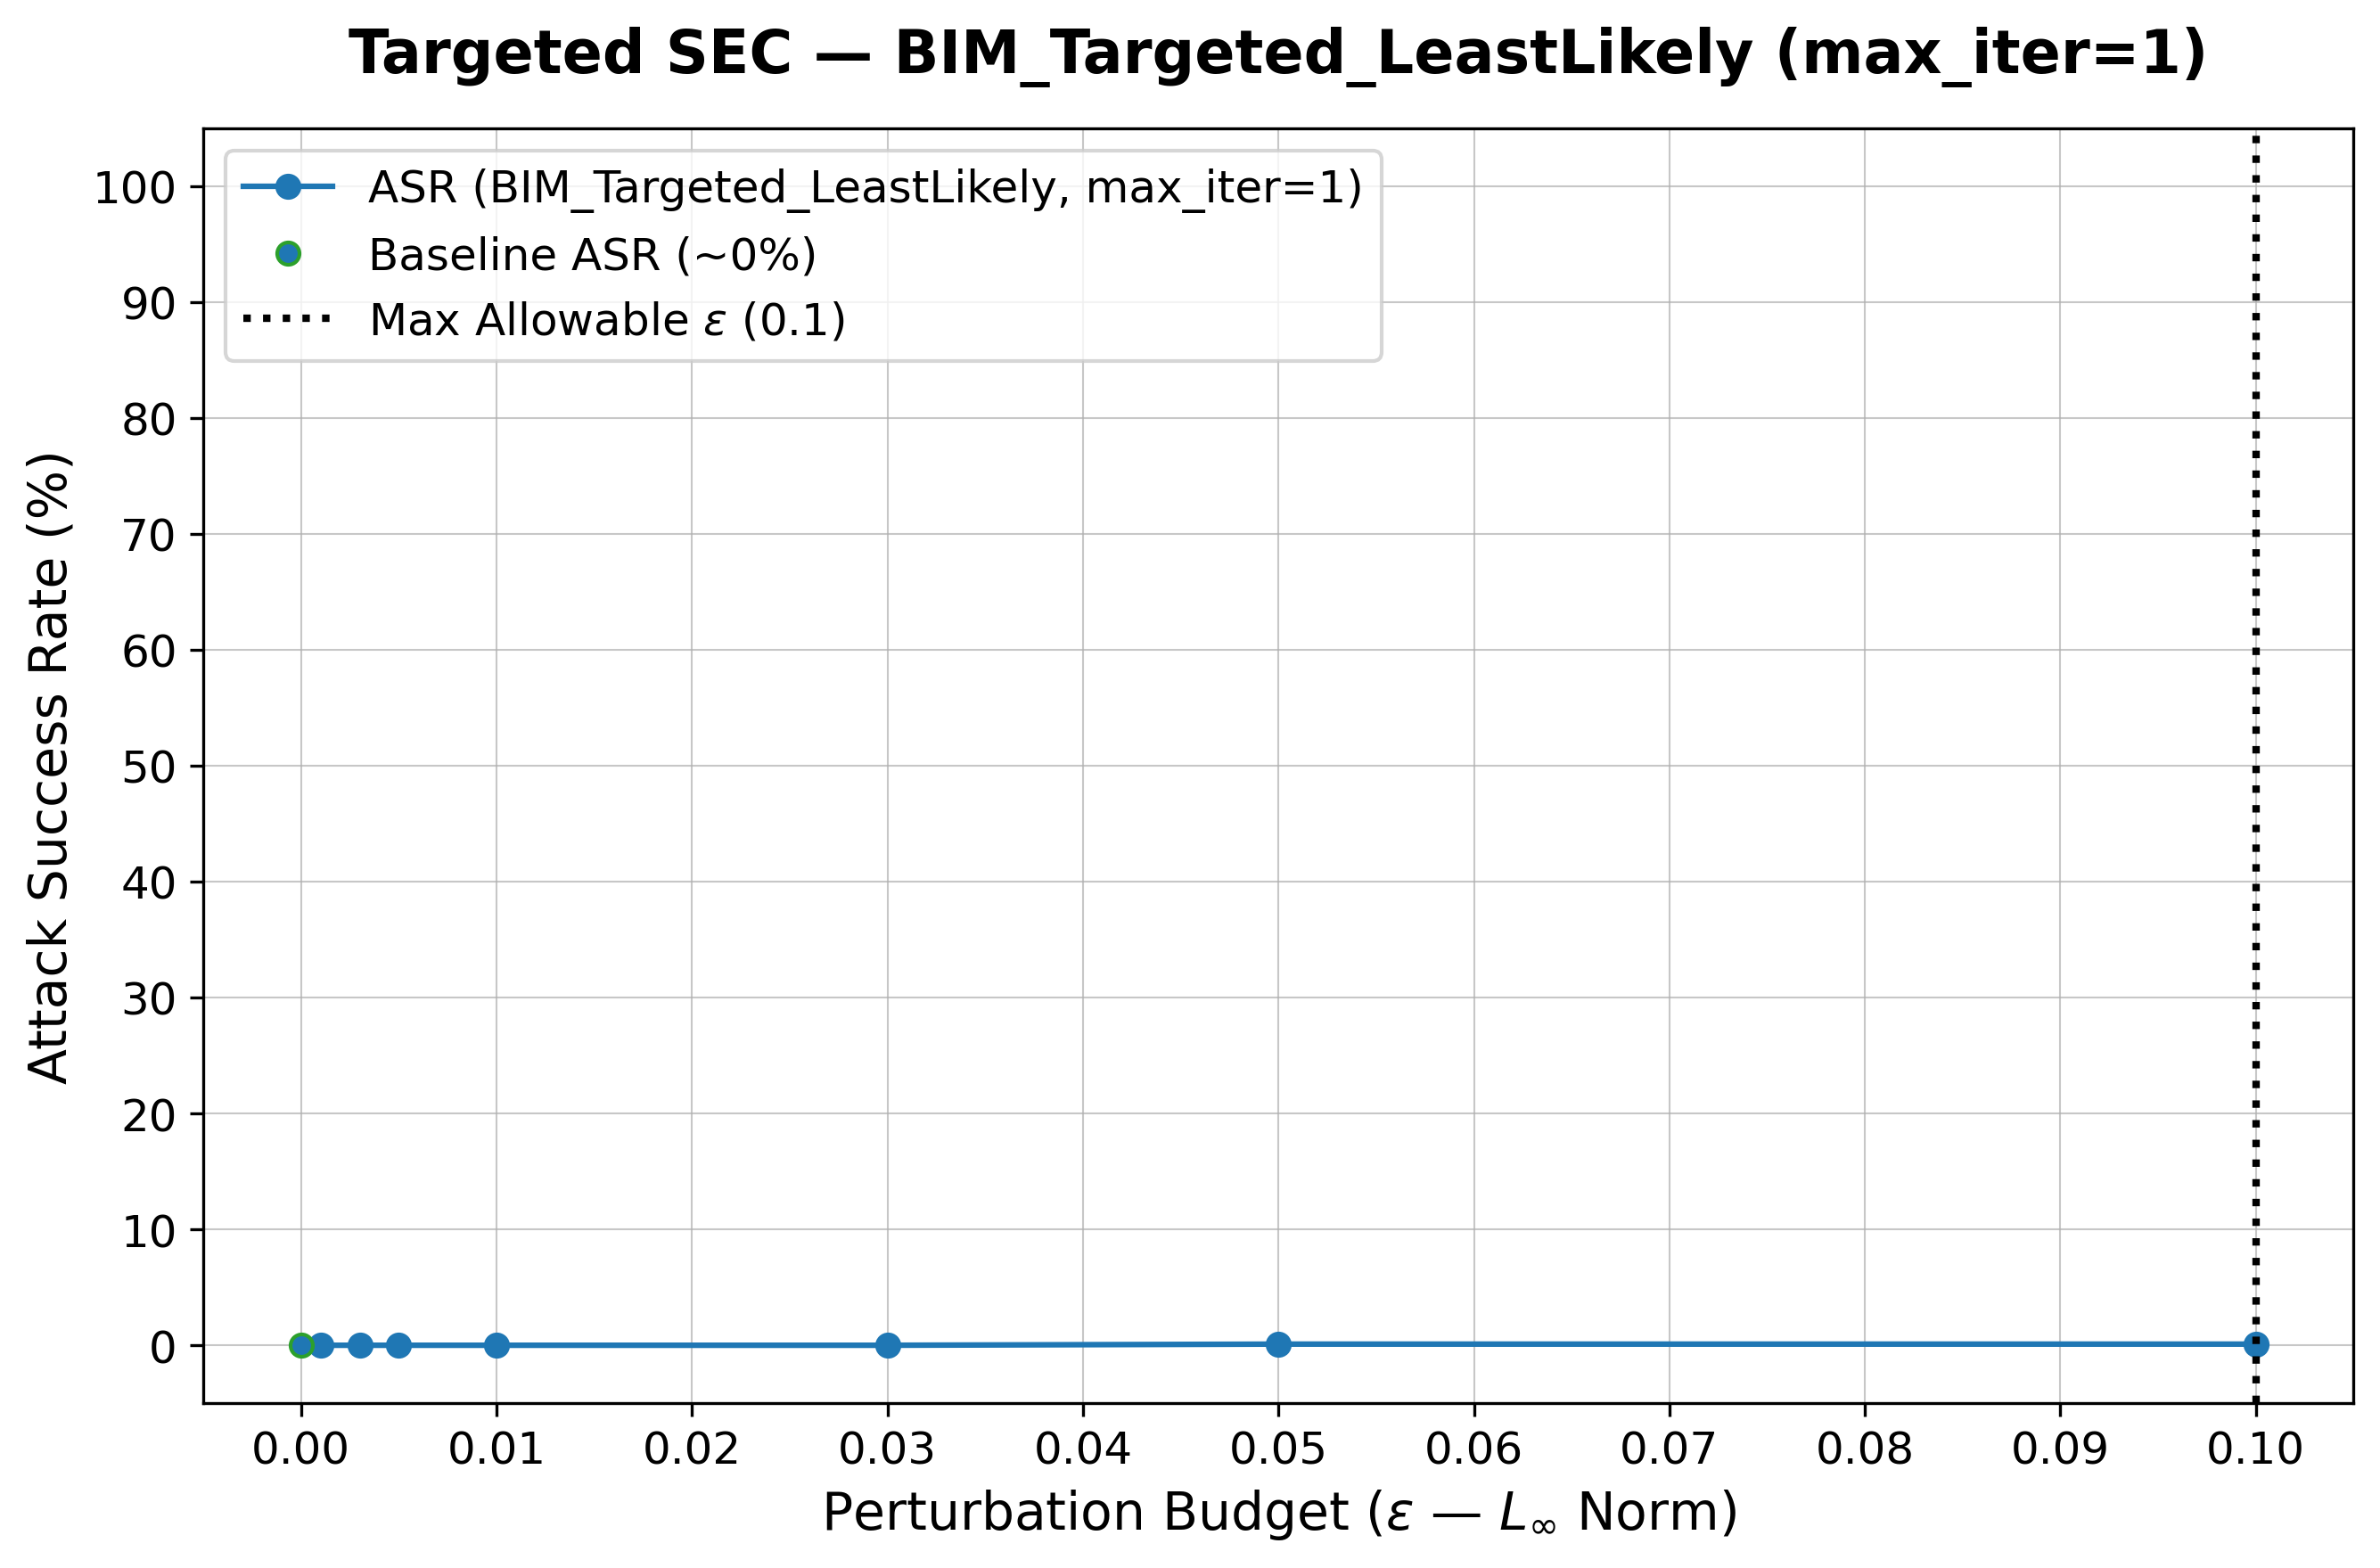
\includegraphics[width=\textwidth]{BIM_Error_specific/LL/BIM_Targeted_LeastLikely_iter1_SEC.png}
                \caption{Iterazione 1}
                \label{fig:iter1_LL}
            \end{subfigure}
            &
            % Prima riga (destra)
            \begin{subfigure}[b]{0.55\textwidth}
                \centering
                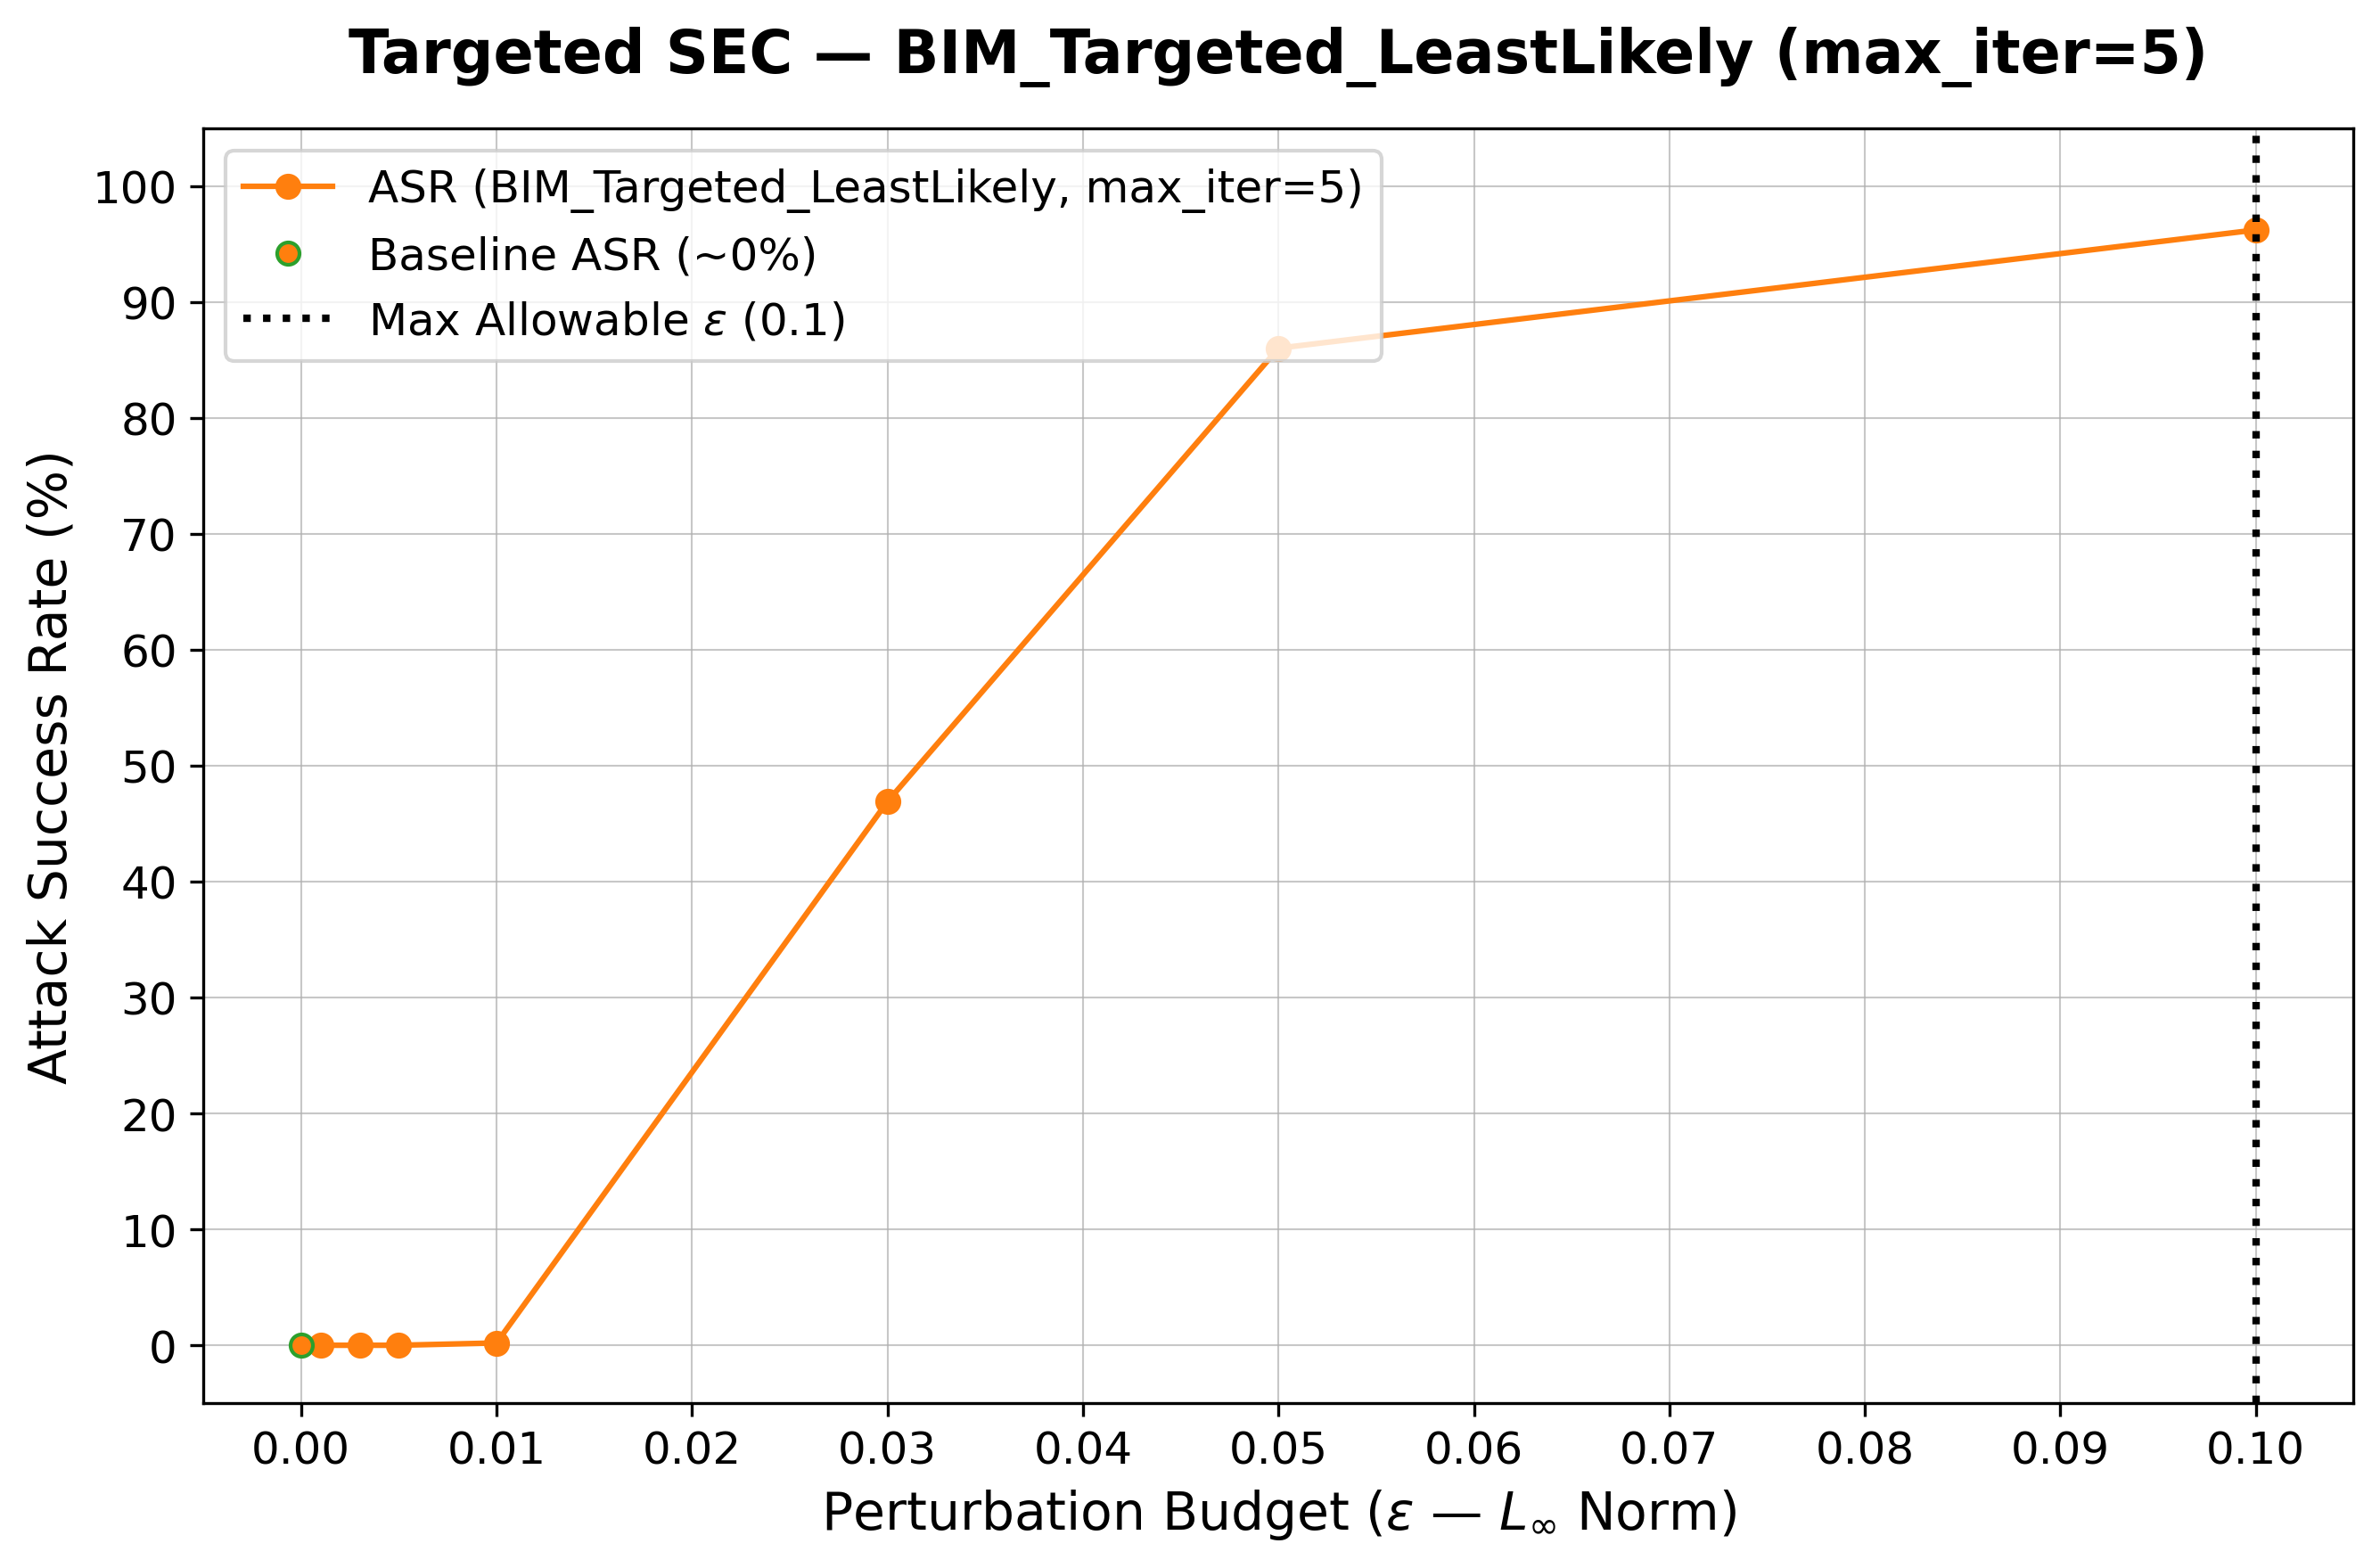
\includegraphics[width=\textwidth]{BIM_Error_specific/LL/BIM_Targeted_LeastLikely_iter5_SEC.png}
                \caption{Iterazione 5}
                \label{fig:iter5_LL}
            \end{subfigure} \\ [0.5cm] % Spazio verticale tra le righe
            
            % Seconda riga (sinistra)
            \begin{subfigure}[b]{0.55\textwidth}
                \centering
                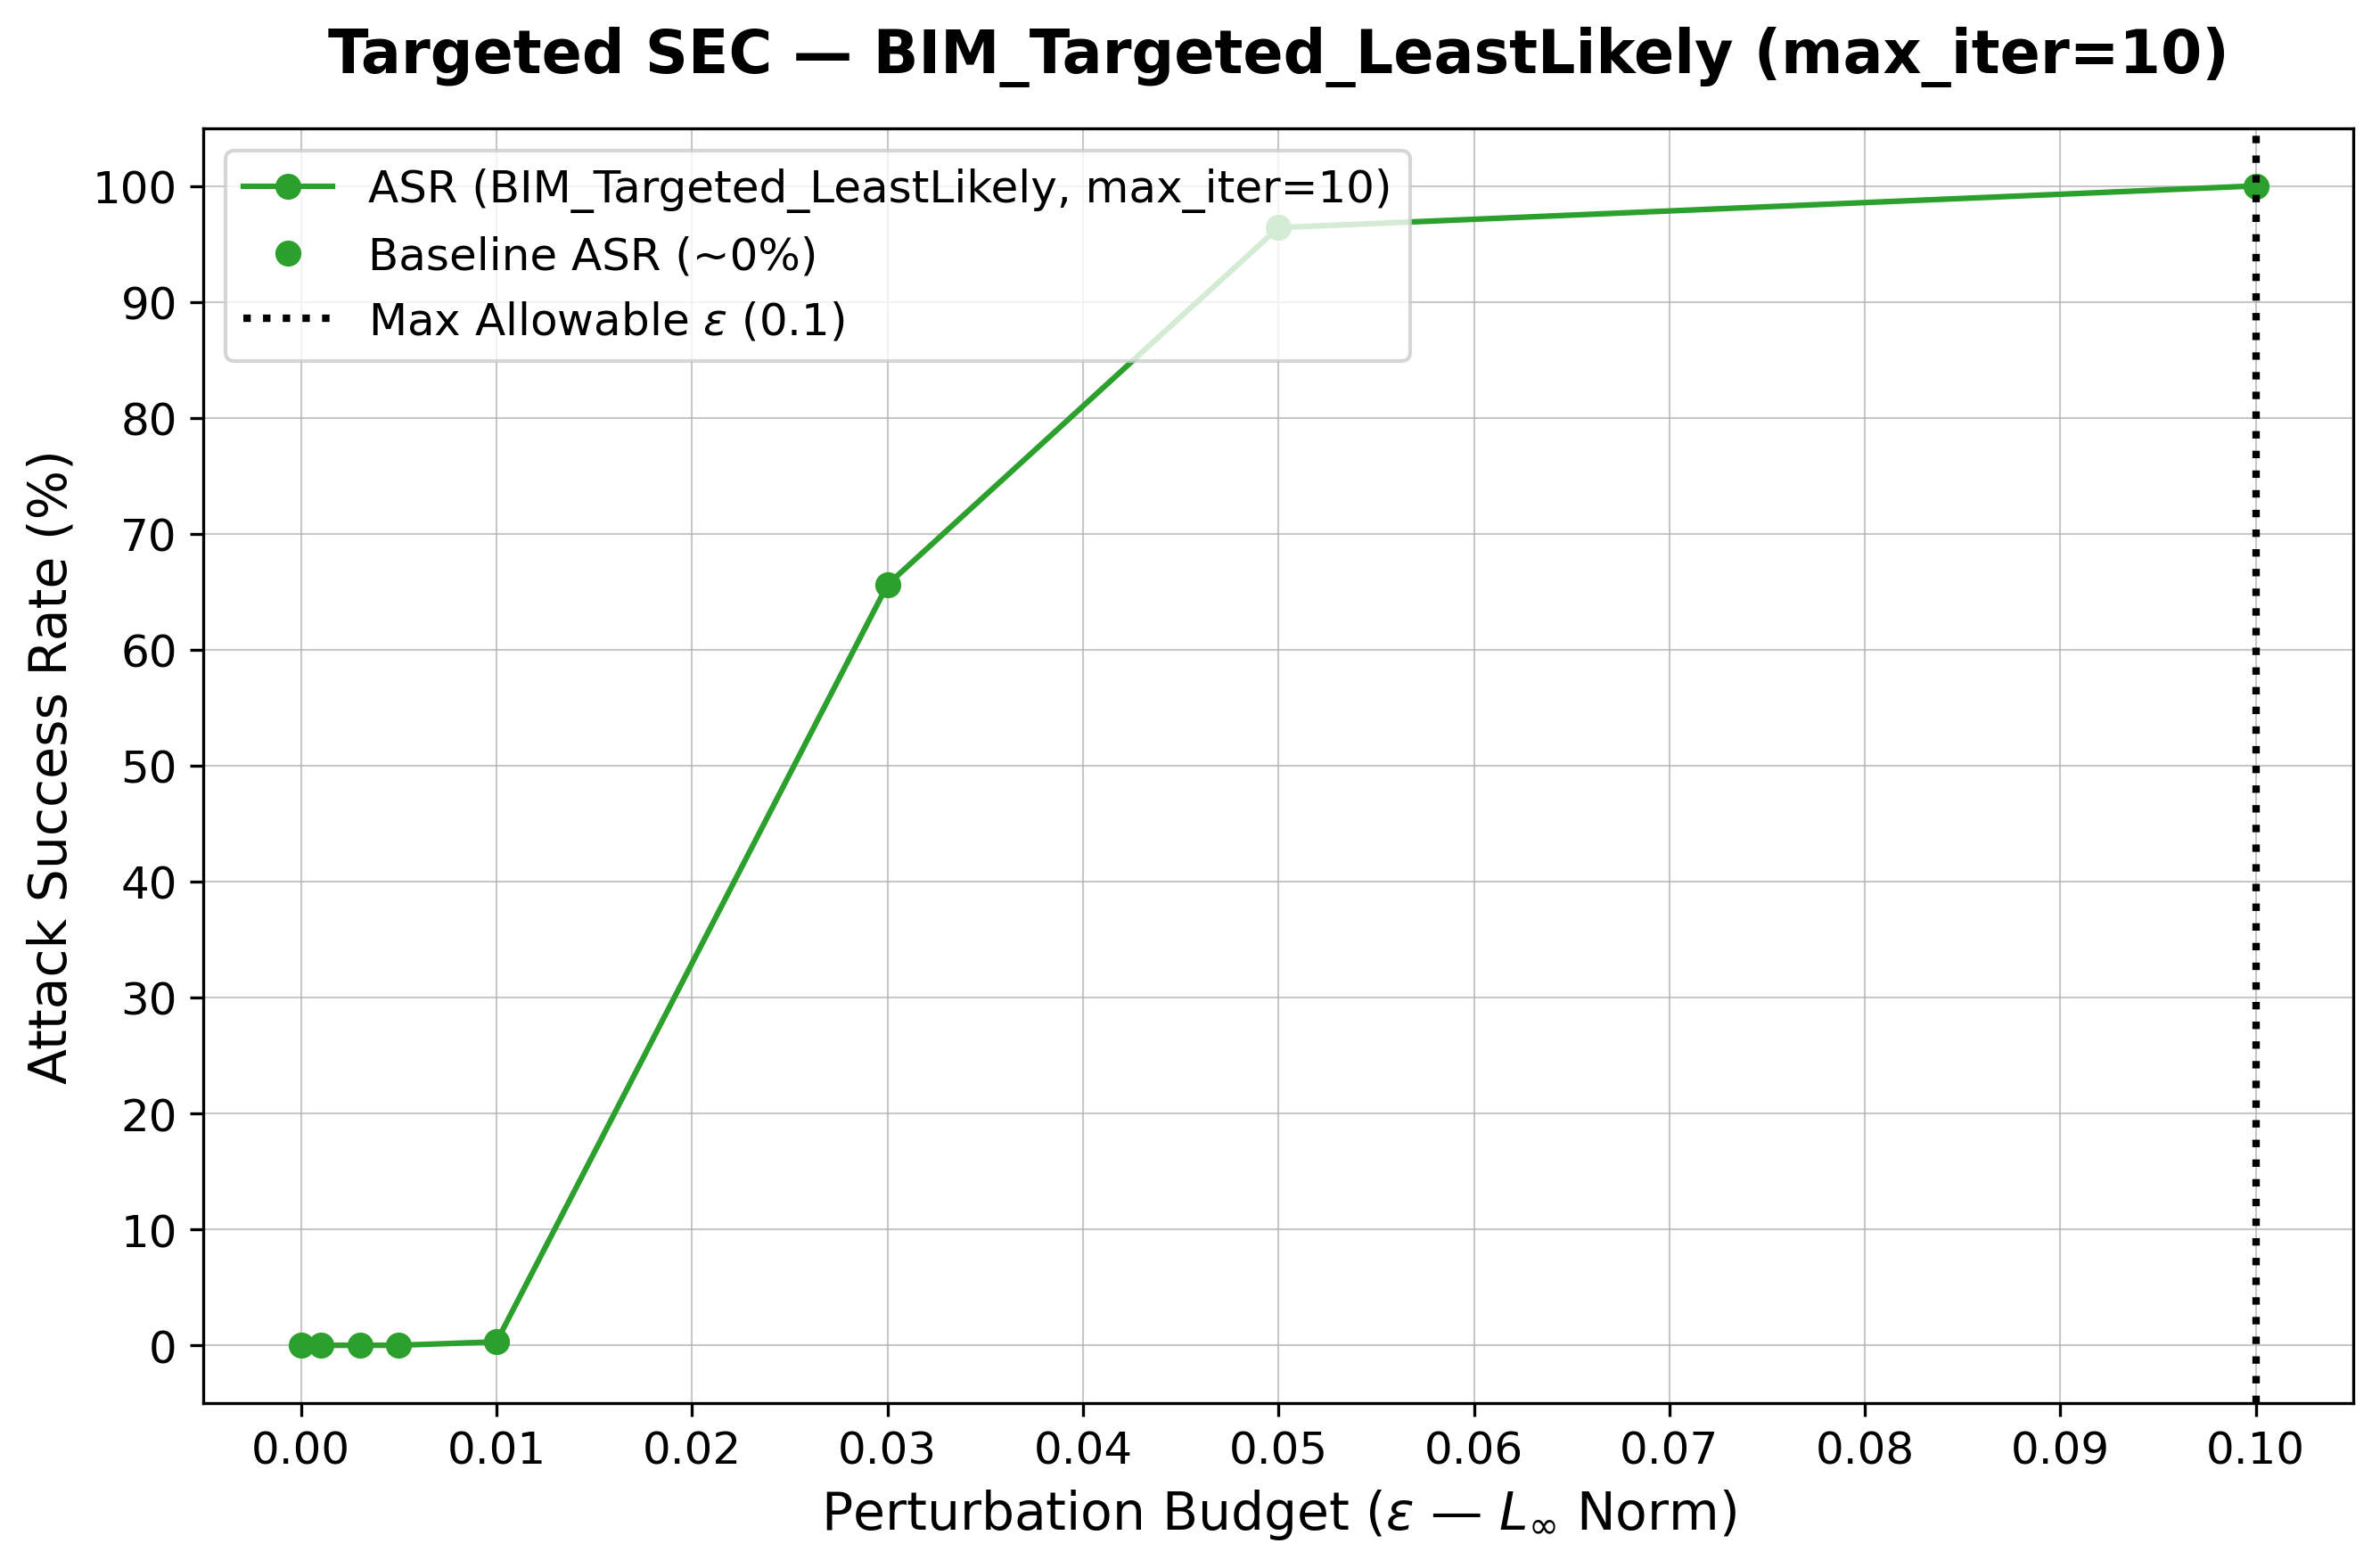
\includegraphics[width=\textwidth]{BIM_Error_specific/LL/BIM_Targeted_LeastLikely_iter10_SEC.png}
                \caption{Iterazione 10}
                \label{fig:iter10_LL}
            \end{subfigure}
            &
            % Seconda riga (destra)
            \begin{subfigure}[b]{0.55\textwidth}
                \centering
                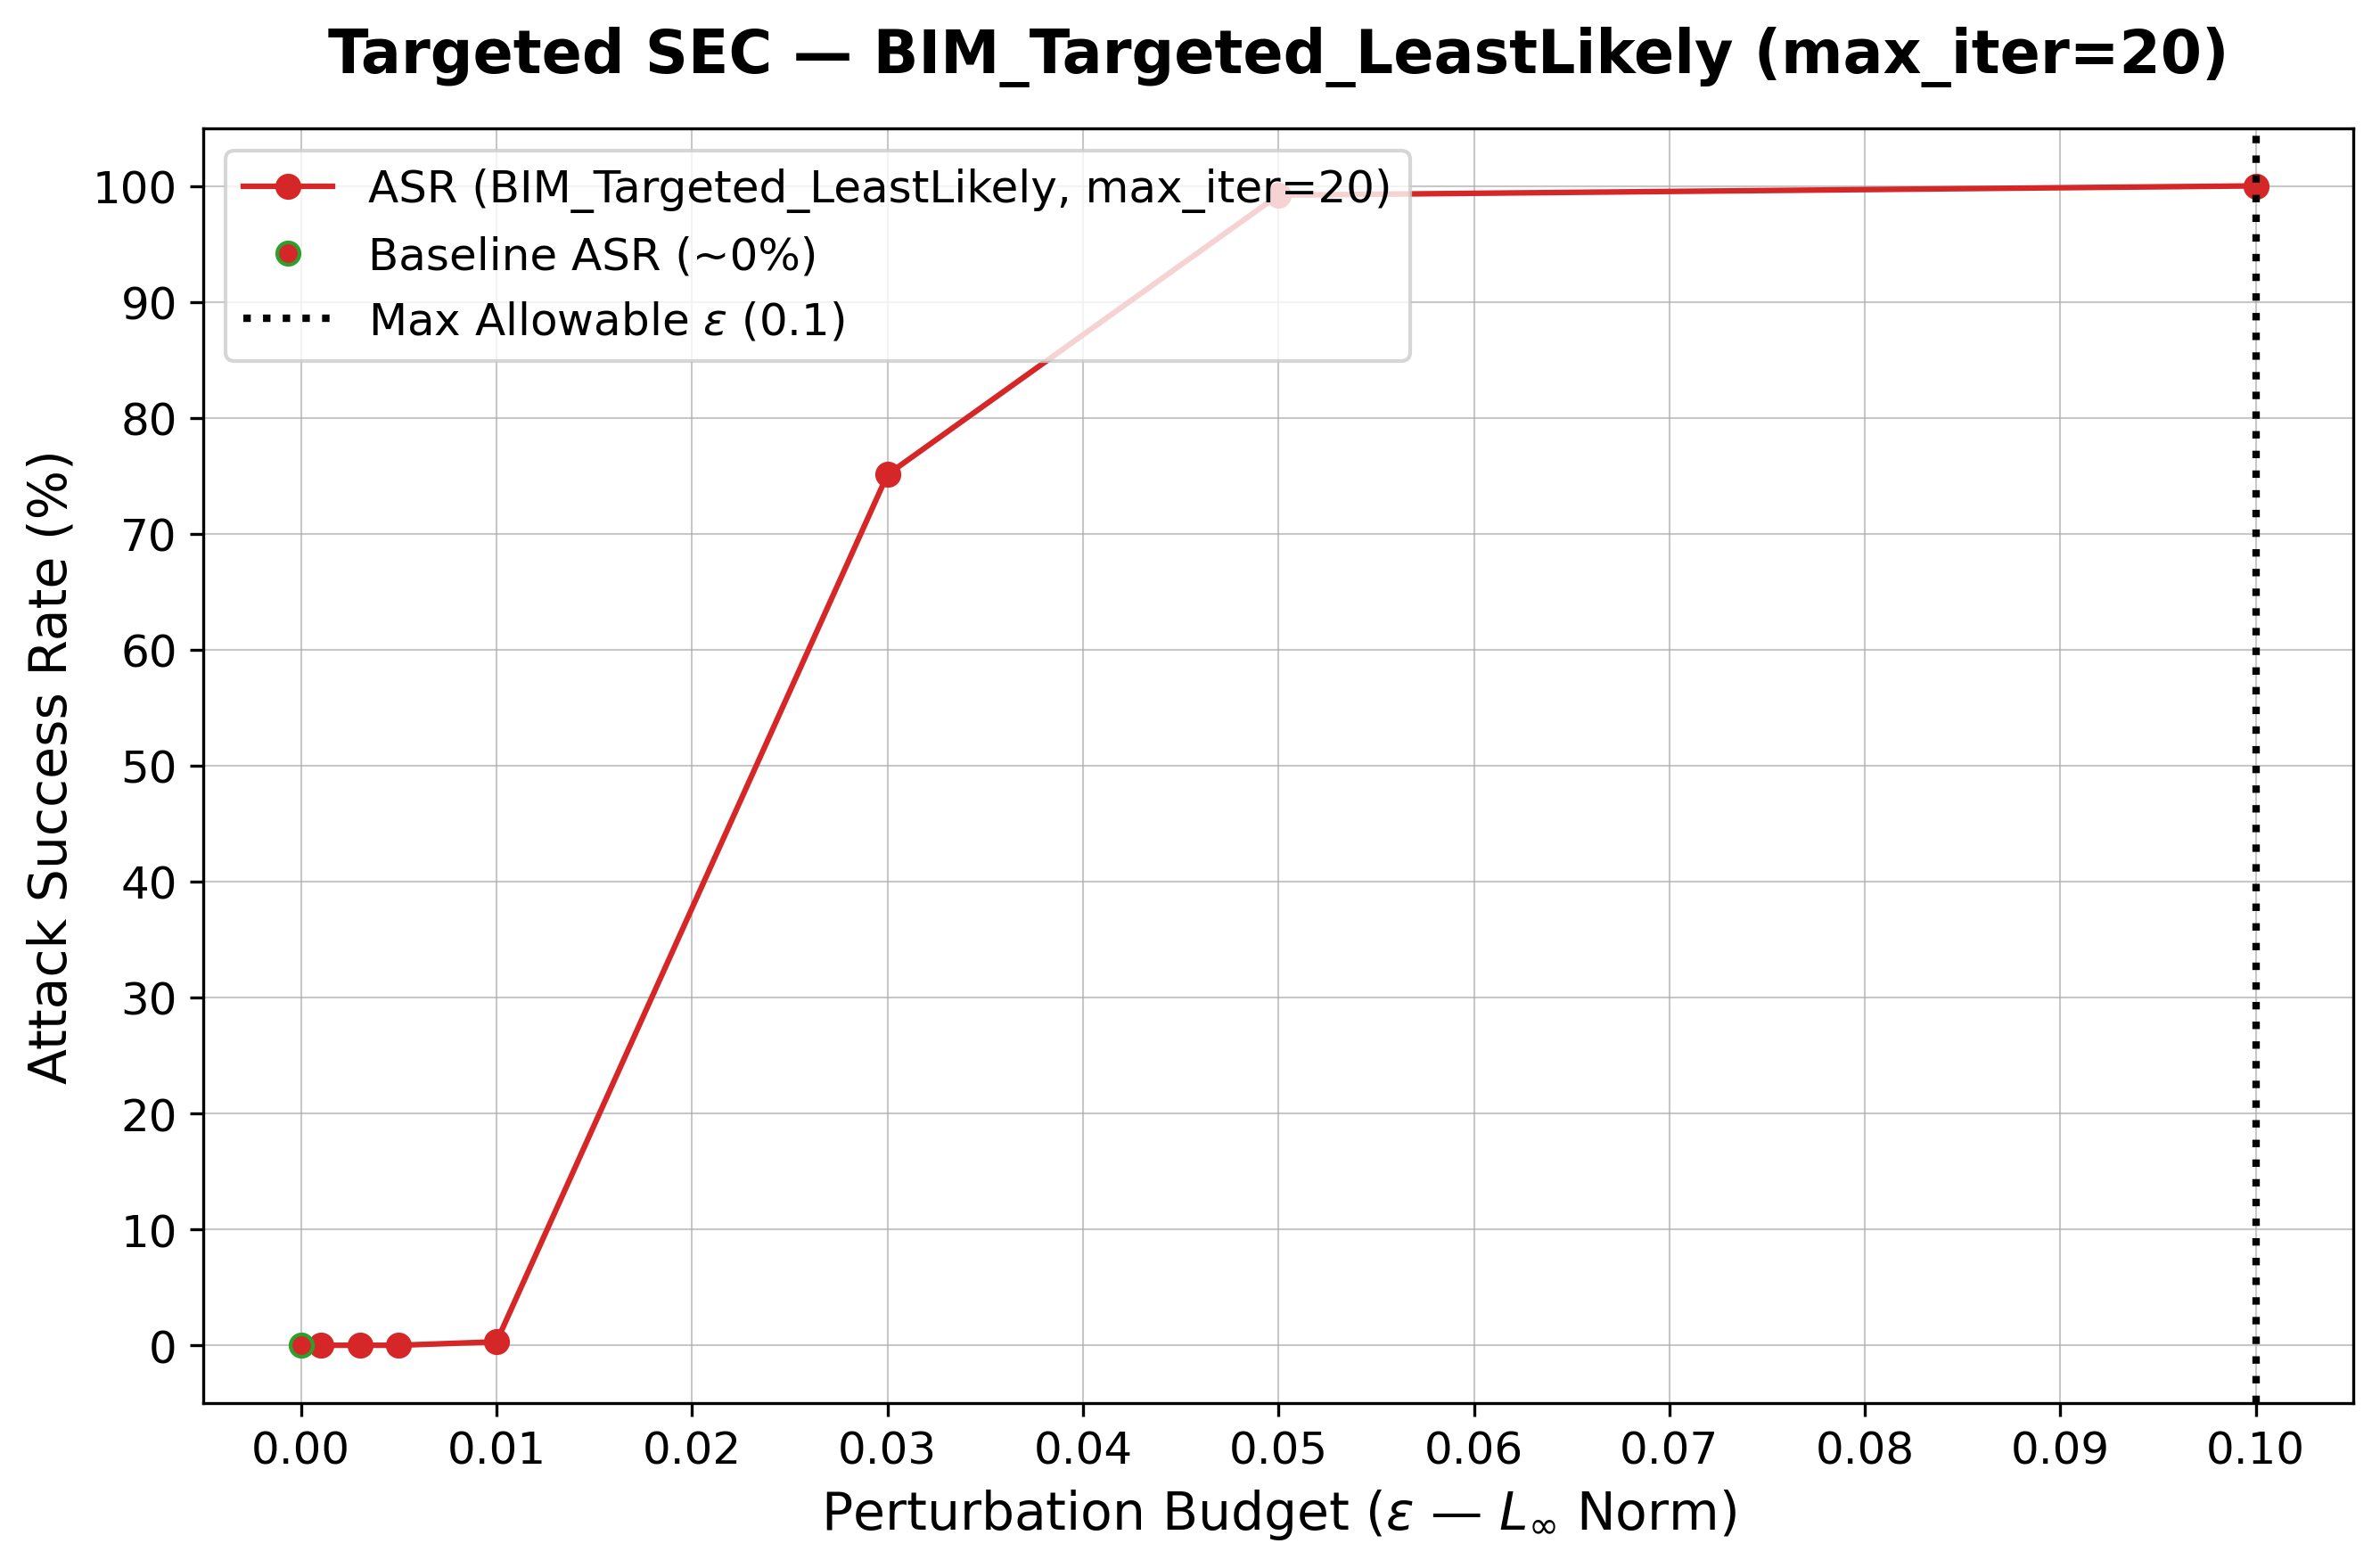
\includegraphics[width=\textwidth]{BIM_Error_specific/LL/BIM_Targeted_LeastLikely_iter20_SEC.png}
                \caption{Iterazione 20}
                \label{fig:iter20_LL}
            \end{subfigure}
            
        \end{tabular}
    }
    
    \caption{Confronto dei risultati al variare delle iterazioni per Least Likely (1, 5, 10 e 20).}
    \label{fig:matrice_iterazioni_LL_BIM}
\end{figure}

\clearpage
\subsubsection{Targeted Projected Gradient Descent (PGD)}
L'algoritmo \textit{Projected Gradient Descent} (PGD), integra una componente stocastica fondamentale: l'inizializzazione casuale (\textit{random restart}).
L'algoritmo prima di iniziare la discesa del gradiente, perturba casualmente il punto di partenza all'interno del \textit{budget} $L_\infty$ consentito.

Esso si sviluppa quindi in due fasi. Inizialmente, si applica lo sbalzo stocastico:
$$ x'_0 = x + \eta \quad \text{con} \quad \eta \sim \mathcal{U}(-\epsilon, \epsilon) $$
Successivamente, si procede con le iterazioni di ottimizzazione verso il target (sottrazione del gradiente) con relativa proiezione di:
$$ x'_t = \Pi_\epsilon \left( x'_{t-1} - \alpha \cdot \text{sign}(\nabla_x \mathcal{L}(h(x'_{t-1}, w), y_{target})) \right) $$
Se la classificazione mirata ha successo in uno qualsiasi dei tentativi previsti dai riavvii casuali, l'attacco si considera riuscito.

Per testare le difese della rete NN1 in modo rigoroso, l'architettura di valutazione ha esplorato una complessa matrice tridimensionale, incrociando:
\begin{itemize}
    \item Il \textit{budget} di perturbazione: $\epsilon \in [0.001, 0.1]$;
    \item La profondità iterativa: \texttt{max\_iter} $\in \{1, 5, 10, 20, 40\}$;
    \item L'esplorazione stocastica: \texttt{num\_random\_init} $\in \{0, 1, 3, 5\}$.
\end{itemize}


\begin{verbatim}
EPSILONS = [0.001, 0.003, 0.005, 0.01, 0.03, 0.05, 0.1]
MAX_ITER_LIST = [1, 5, 10, 20, 40]
NUM_RANDOM_INITS = [0, 1, 3, 5]

\end{verbatim}

È fondamentale notare che la configurazione con \texttt{num\_random\_init} = 0 annulla l'inizializzazione stocastica, riducendo il PGD a un attacco BIM standard, fornendo così un metro di paragone interno.

Le sezioni a seguire conterranno un'analisi quantitativa granulare basata sulle \textit{Targeted SEC}, al fine di isolare l'efficacia dei singoli iperparametri (iterazioni \textit{vs.} riavvii casuali) sull'\textit{Attack Success Rate} complessivo. Al fine di non appesantire ulteriormente la lettura dell'elaborato, è possibile consultare i valori precisi dei risultati empirici ottenuti durante la fase di test, alle   seguenti cartelle:
\begin{itemize}
    \item \href{https://github.com/ChristianRosa02/AI4Cybersecurity/blob/master/results/PGD_Targeted_Fixed/PGD_Targeted_Fixed_results.csv}{risultati fixed}
    \item \href{https://github.com/ChristianRosa02/AI4Cybersecurity/blob/master/results/PGD_Targeted_LeastLikely/PGD_Targeted_LeastLikely_results.csv}{risultati Least Likely}
\end{itemize}

\clearpage
\subsubsection*{Fixed Attack}
Per valutare l'effettivo apporto del PGD, è necessario confrontare le prestazioni ottenute abilitando l'inizializzazione stocastica (\texttt{num\_random\_init} $> 0$) con la \textit{baseline} algoritmica priva di rumore iniziale (\texttt{num\_random\_init} $= 0$, equivalente al BIM).

Il dato più interessante, si manifesta analizzando l'impatto dei \textit{random restart}. Contrariamente a quanto si possa pensare, nei test a bersaglio fisso l'introduzione dei riavvii casuali produce un \textbf{degrado prestazionale} della capacità offensiva. Estraendo i dati dal CSV per \textit{budget} intermedi, si osserva che a $\epsilon = 0.03$ (con 10 iterazioni), la configurazione \texttt{nri} = 0 garantisce un ASR del 96.8\%, mentre l'attivazione di 5 \textit{random restart} fa calare l'ASR al 90.6\%. Analogamente, a $\epsilon = 0.01$, il tasso di successo scende dal 18.6\% (senza riavvii) al 7.8\% (con 5 riavvii).

La spiegazione di questo fenomeno risiede nella natura del \textit{targeted attack} verso una classe specifica. La regione di pertinenza della classe bersaglio è stretta e ben localizzata nello spazio delle \textit{feature}. L'approccio deterministico (BIM) calcola immediatamente il percorso più diretto e ottimizzato dall'immagine originale verso tale regione. Al contrario, il PGD applica un salto casuale iniziale: questa perturbazione alla cieca rischia di spingere il vettore in una porzione di spazio peggiore rispetto alla groud truth. 

A questa penalizzazione si somma un aumento in termini di costo computazionale. L'esecuzione di 5 \textit{random restart} moltiplica il numero di inferenze. Ad esempio, per la configurazione con 10 iterazioni e $\epsilon=0.03$, l'elaborazione deterministica ha richiesto circa 39.19 secondi, contro i 200 secondi della variante stocastica (\texttt{nri} = 5), senza alcun beneficio in termini di ASR finale. 

In definitiva, l'analisi evidenzia che, a parità di iterazioni e \textit{budget}, l'attacco PGD in modalità \textit{Fixed} non apporta alcun miglioramento in termini di \textit{Attack Success Rate} rispetto alla sua controparte puramente deterministica (BIM). 

In tabella~\ref{tab:PGD_fixed}, è riportata in maniera più compatta l'analisi quantitativa svolta in precedenza.Sono riportati svariati grafici che mettono a confronto l'impatto dei parametri di PGD. Ogni grafico è seguito da sottografici che consentono una visualizzazione più pulita delle curve di interesse.
Inoltre, per aiutare una comparazione visiva più immediata, è stata realizzata in figura~\ref{fig:PGD_iterations_vari_nri} una matrice di immagini che affianca le 4 SEC realizzate al variare di \texttt{max\_iter} (1, 5, 10, 20 e 40) per tutte le \texttt{nri} previste. 

\begin{table}[h]
    \centering
    \begin{tabular}{ccccc}
    \toprule
        \textbf{nri} & \textbf{max_iter} & $\boldsymbol{\epsilon}$ & \textbf{ASR (\%)} & \textbf{Time (s)} \\
        \midrule
        0 & 10 & 0.001 & 0.0 & 41.38\\
        0 & 10 & 0.003 & 0.1 & 41.71\\
        0 & 10 & 0.005 & 1.0 & 41.84\\
        0 & 10 & 0.01 & 18.6 & 41.47\\
        \textbf{0} & \textbf{10} & \textbf{0.03} & \textbf{96.8} & \textbf{39.19}\\
        5 & 10 & 0.001 & 0.0 & 204.77\\
        5 & 10 & 0.003 & 0.0 & 166.10\\
        5 & 10 & 0.005 & 0.4 & 208.01\\
        5 & 10 & 0.01 & 7.8 & 163.94\\
        5 & 10 & 0.03 & 90.6 & 200.40\\
    \bottomrule
    \end{tabular}
    \caption{Vista ridotta per l'analisi quantitativa di PGD Fixed}
    \label{tab:PGD_fixed}
\end{table}

Poiché la formulazione teorica di PGD suggeriva un potenziale vantaggio offensivo, l'indagine è stata estesa a una valutazione qualitativa degli esempi avversari generati, al fine di misurarne la furtività agli occhi di un osservatore umano. A tal proposito, la figura~\ref{fig:BIM_PGD_Compare} offre un riscontro visivo diretto: essa affianca l'immagine originale pulita (relativa al soggetto \textit{n0001} del dataset) alle rispettive versioni alterate da BIM e PGD, a parità di \texttt{max\_iter} ed $\epsilon$. Questo parallelismo empirico consente di apprezzare le differenze nella distribuzione spaziale del rumore e di valutare se la componente stocastica introdotta da PGD renda la perturbazione meno sospetta e riconoscibile rispetto a BIM.

% INSERIRE FOTO COMPARATIVE
\textbf{INSERIRE FOTO COMPARATIVE BIM VS PGD}




\clearpage
% -- SEC NRI = 0 -- 
\begin{figure}[H]
    \centering
    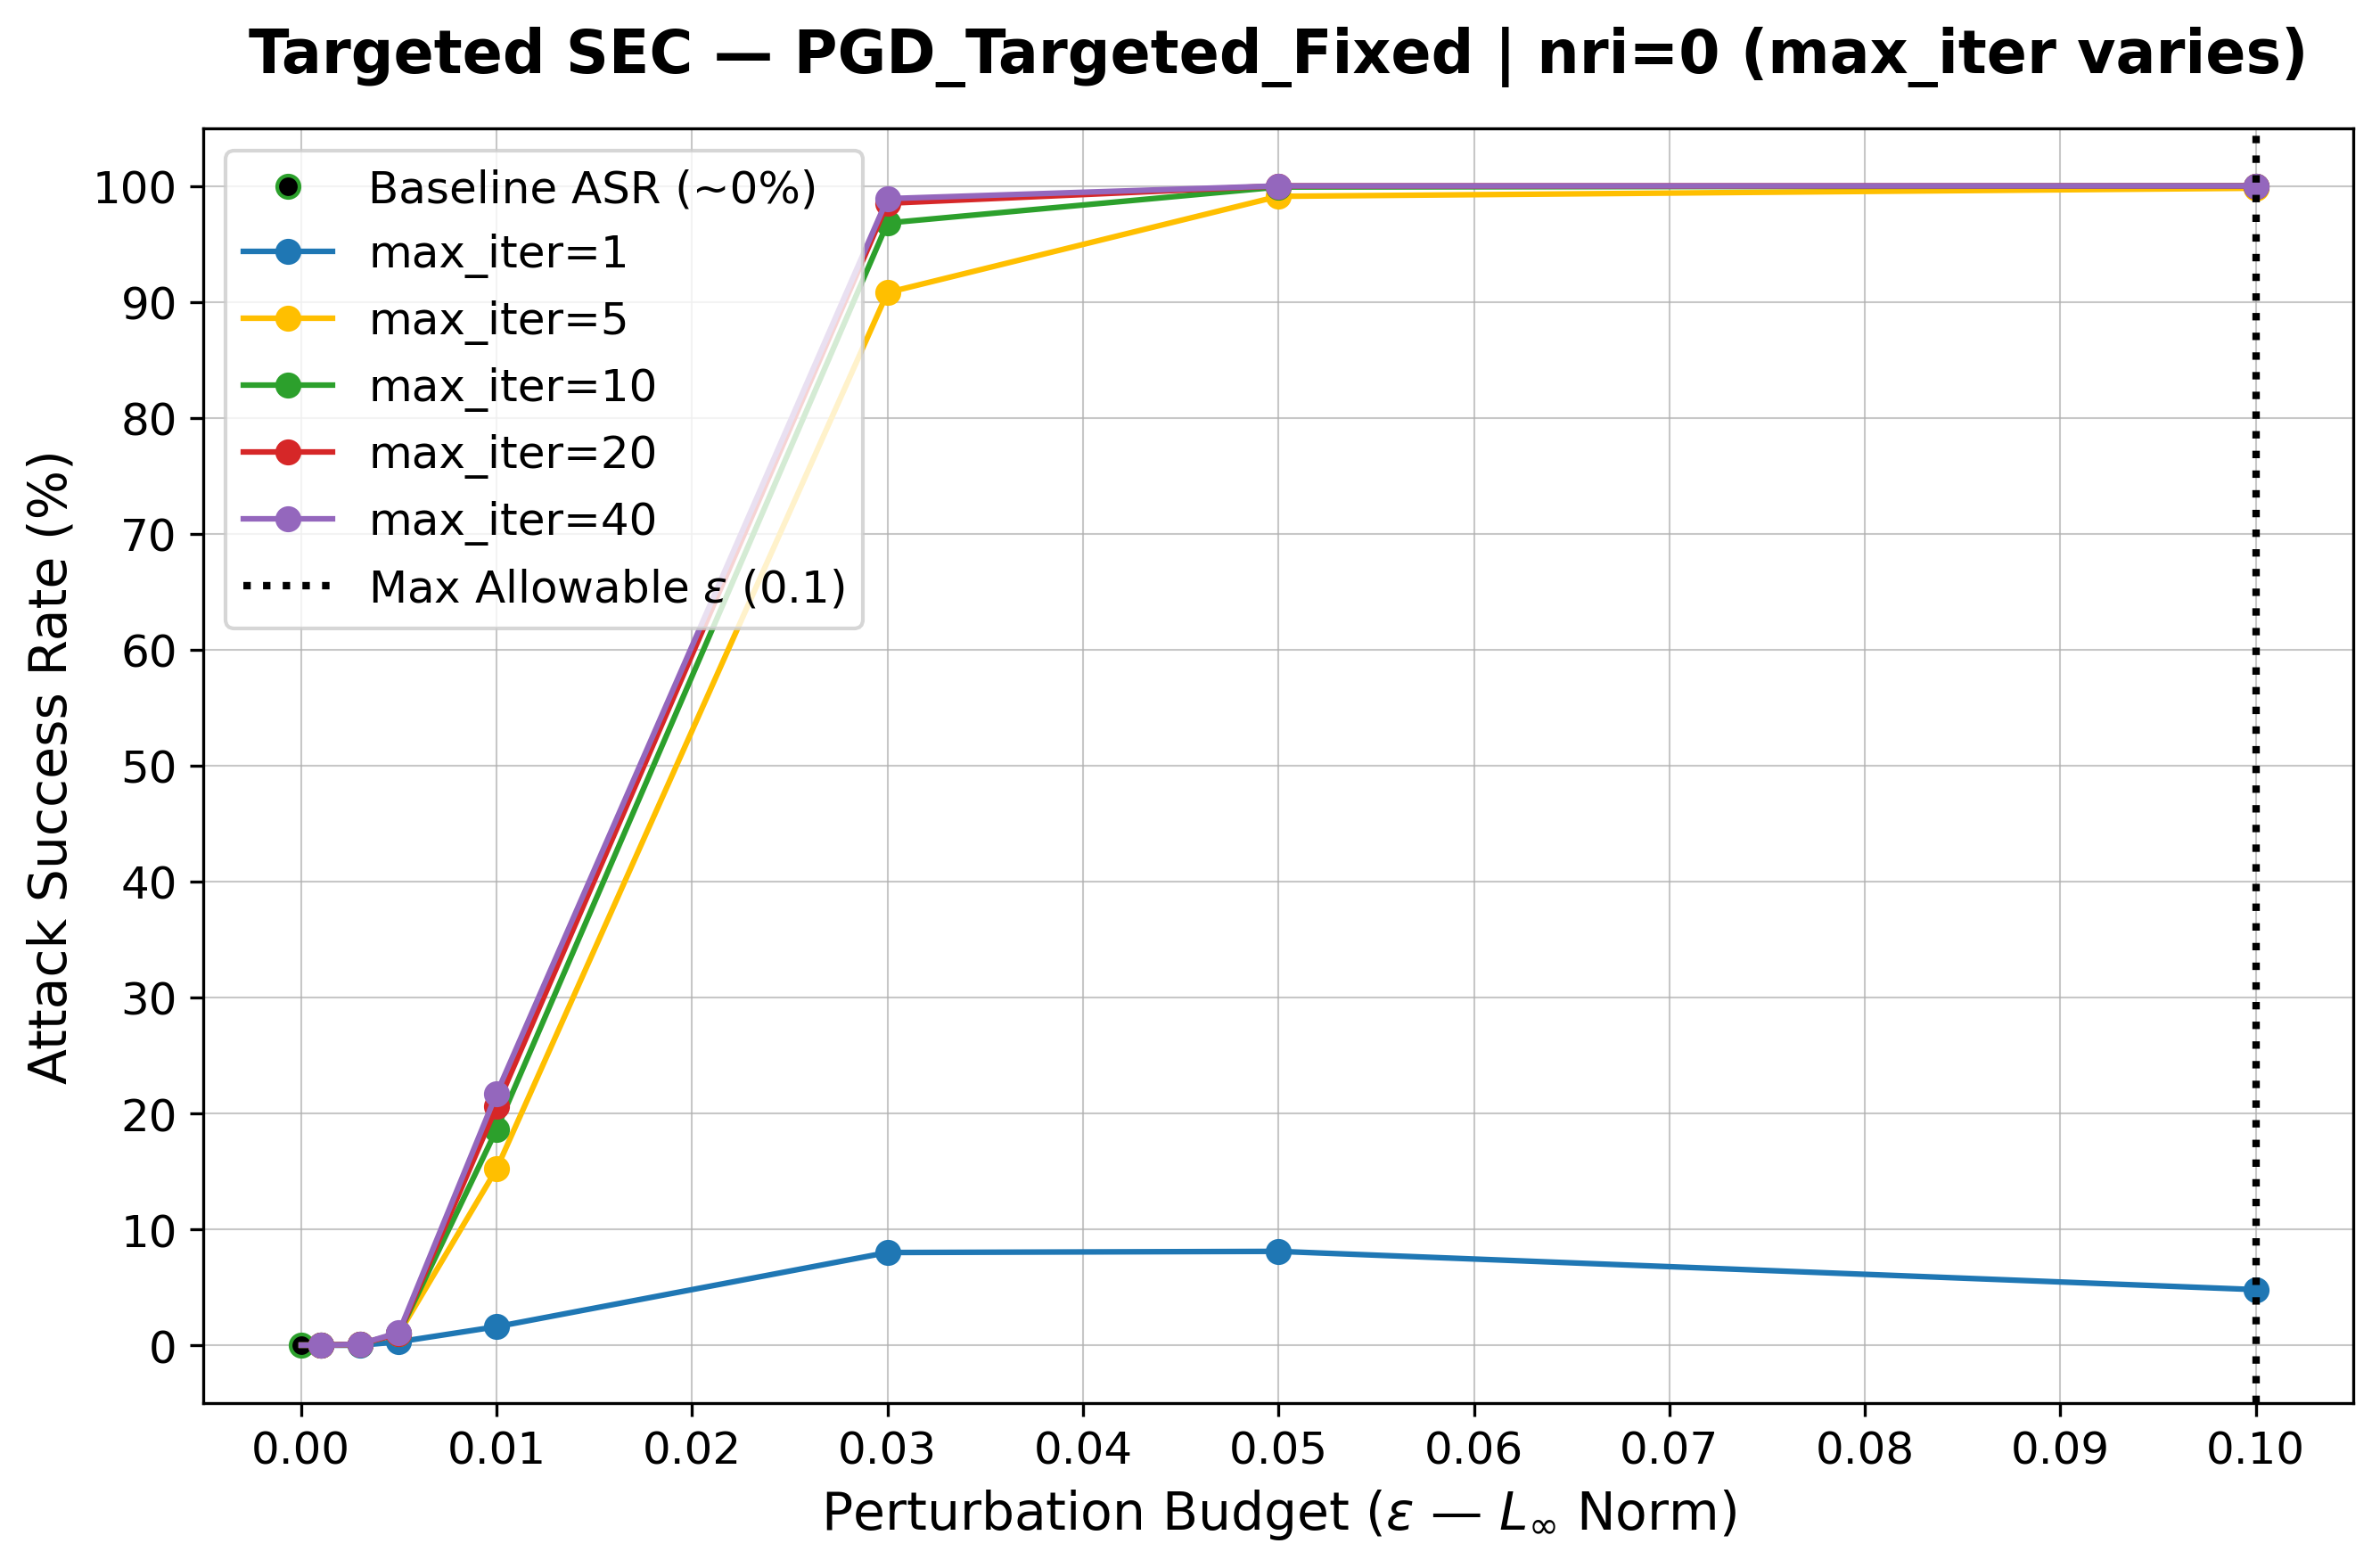
\includegraphics[width=0.5\linewidth]{PGD_Error_specific/Fixed/PGD_Targeted_Fixed_nri0_comparative_maxiter_SEC.png}
    \caption{PGD SEC con nri = 0}
    \label{fig:PGD_SEC_nri0}
\end{figure}

% -- SOTTO GRAFICI PER NRI = 0
\begin{figure}[H]
    \centering
    % Sotto-figura 1
    \begin{subfigure}[b]{0.45\textwidth}
        \centering
        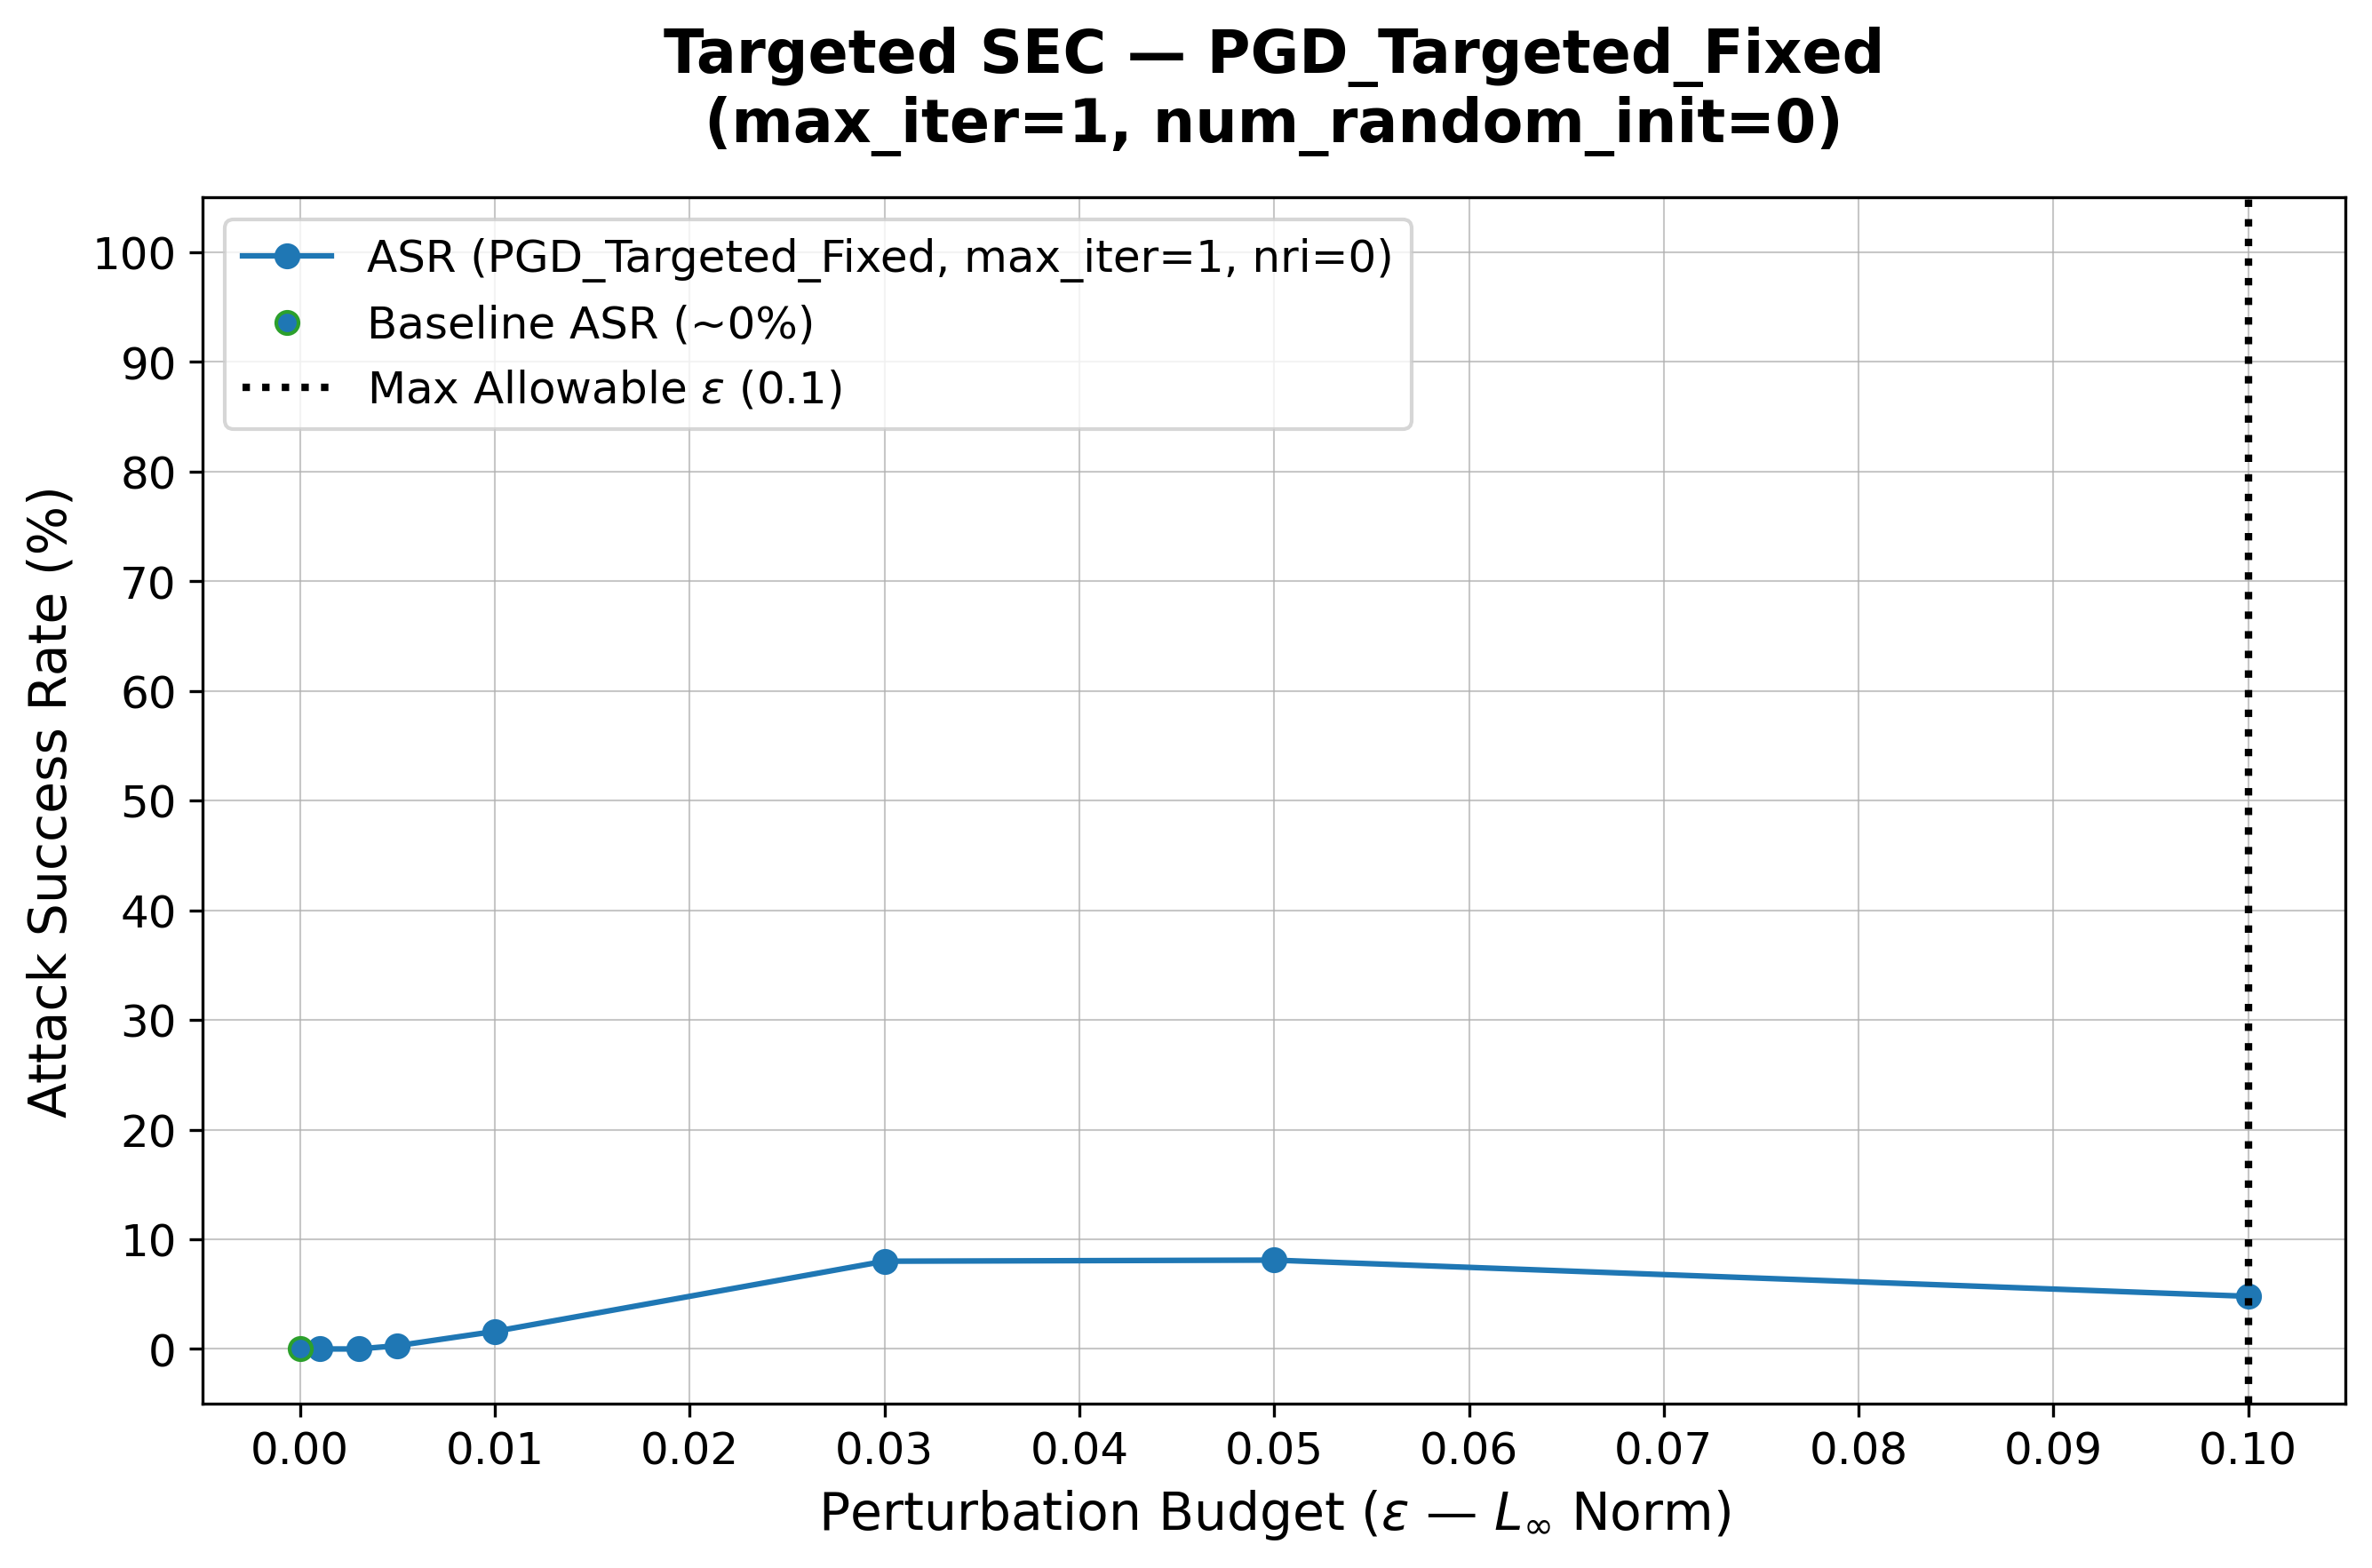
\includegraphics[width=\textwidth]{PGD_Error_specific/Fixed/PGD_Targeted_Fixed_nri0_iter1_SEC.png}
        \caption{\texttt{max_iter} = 1}
        \label{fig:PGD_iter1}
    \end{subfigure}
    \hfill
    % Sotto-figura 2
    \begin{subfigure}[b]{0.45\textwidth}
        \centering
        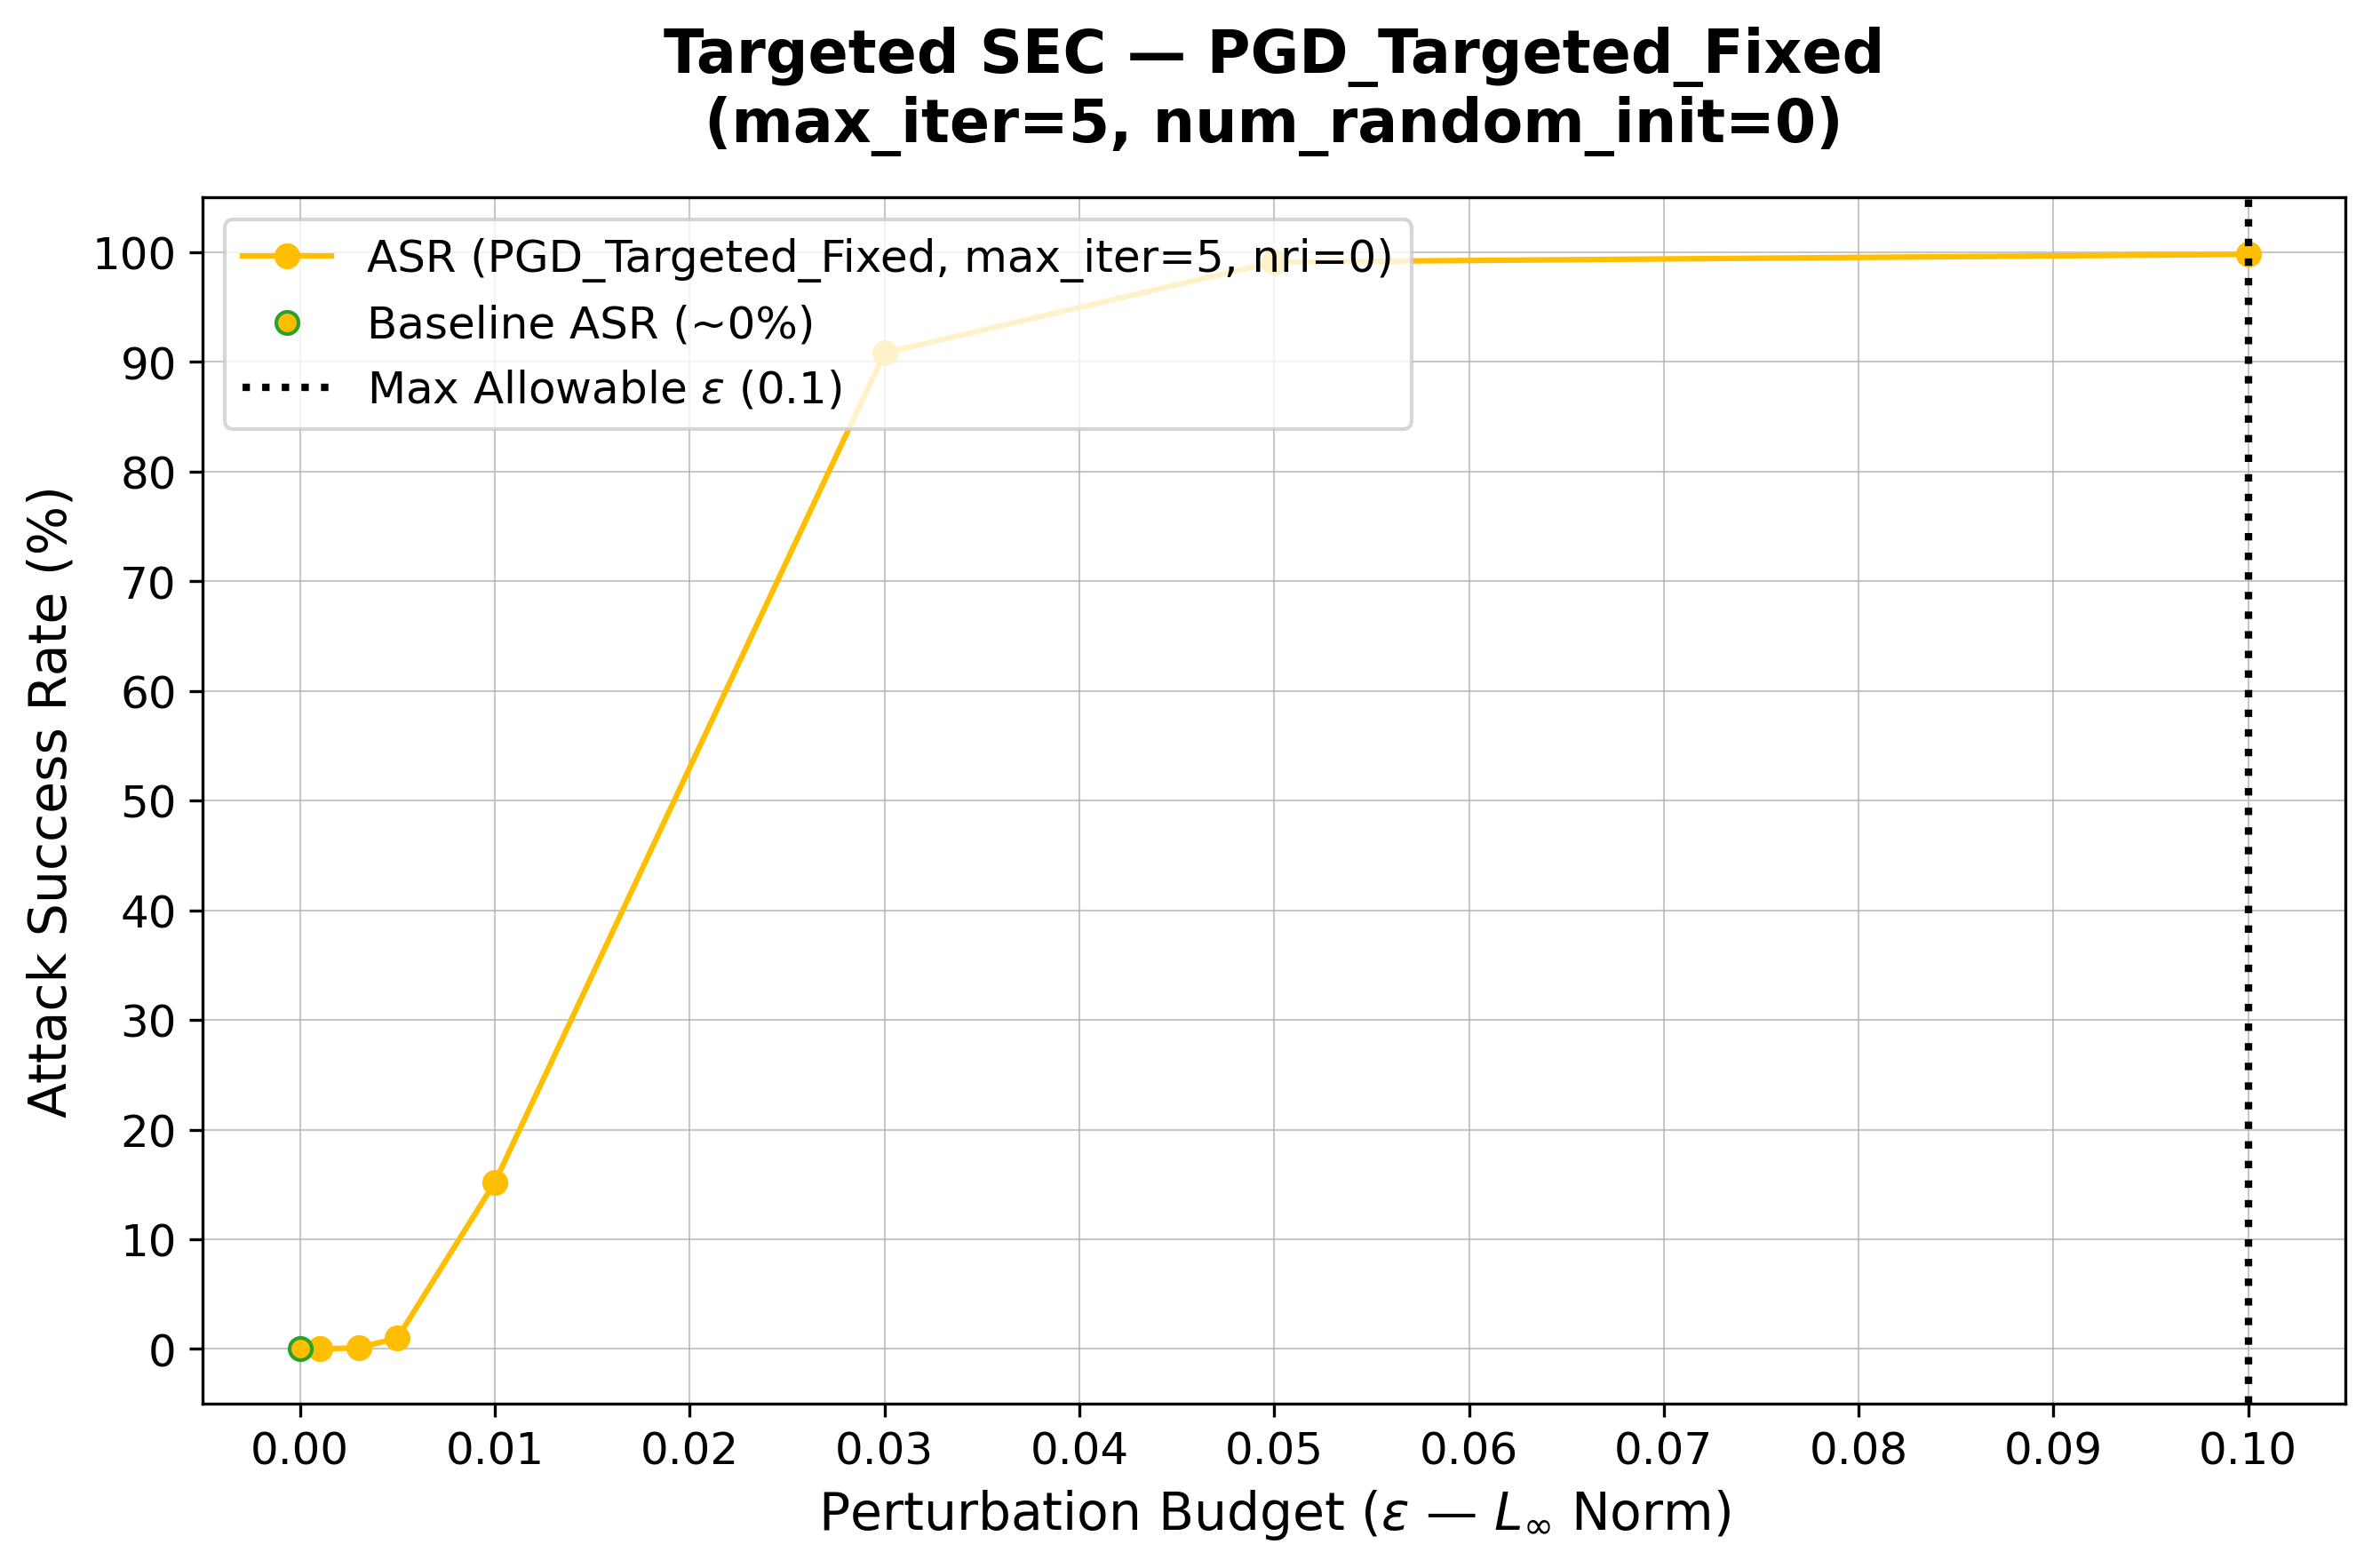
\includegraphics[width=\textwidth]{PGD_Error_specific/Fixed/PGD_Targeted_Fixed_nri0_iter5_SEC.png}
        \caption{\texttt{max_iter} = 5}
        \label{fig:PGD_iter5}
    \end{subfigure}

    \vspace{1em} % Spazio verticale tra le righe di immagini

    % Sotto-figura 3
    \begin{subfigure}[b]{0.45\textwidth}
        \centering
        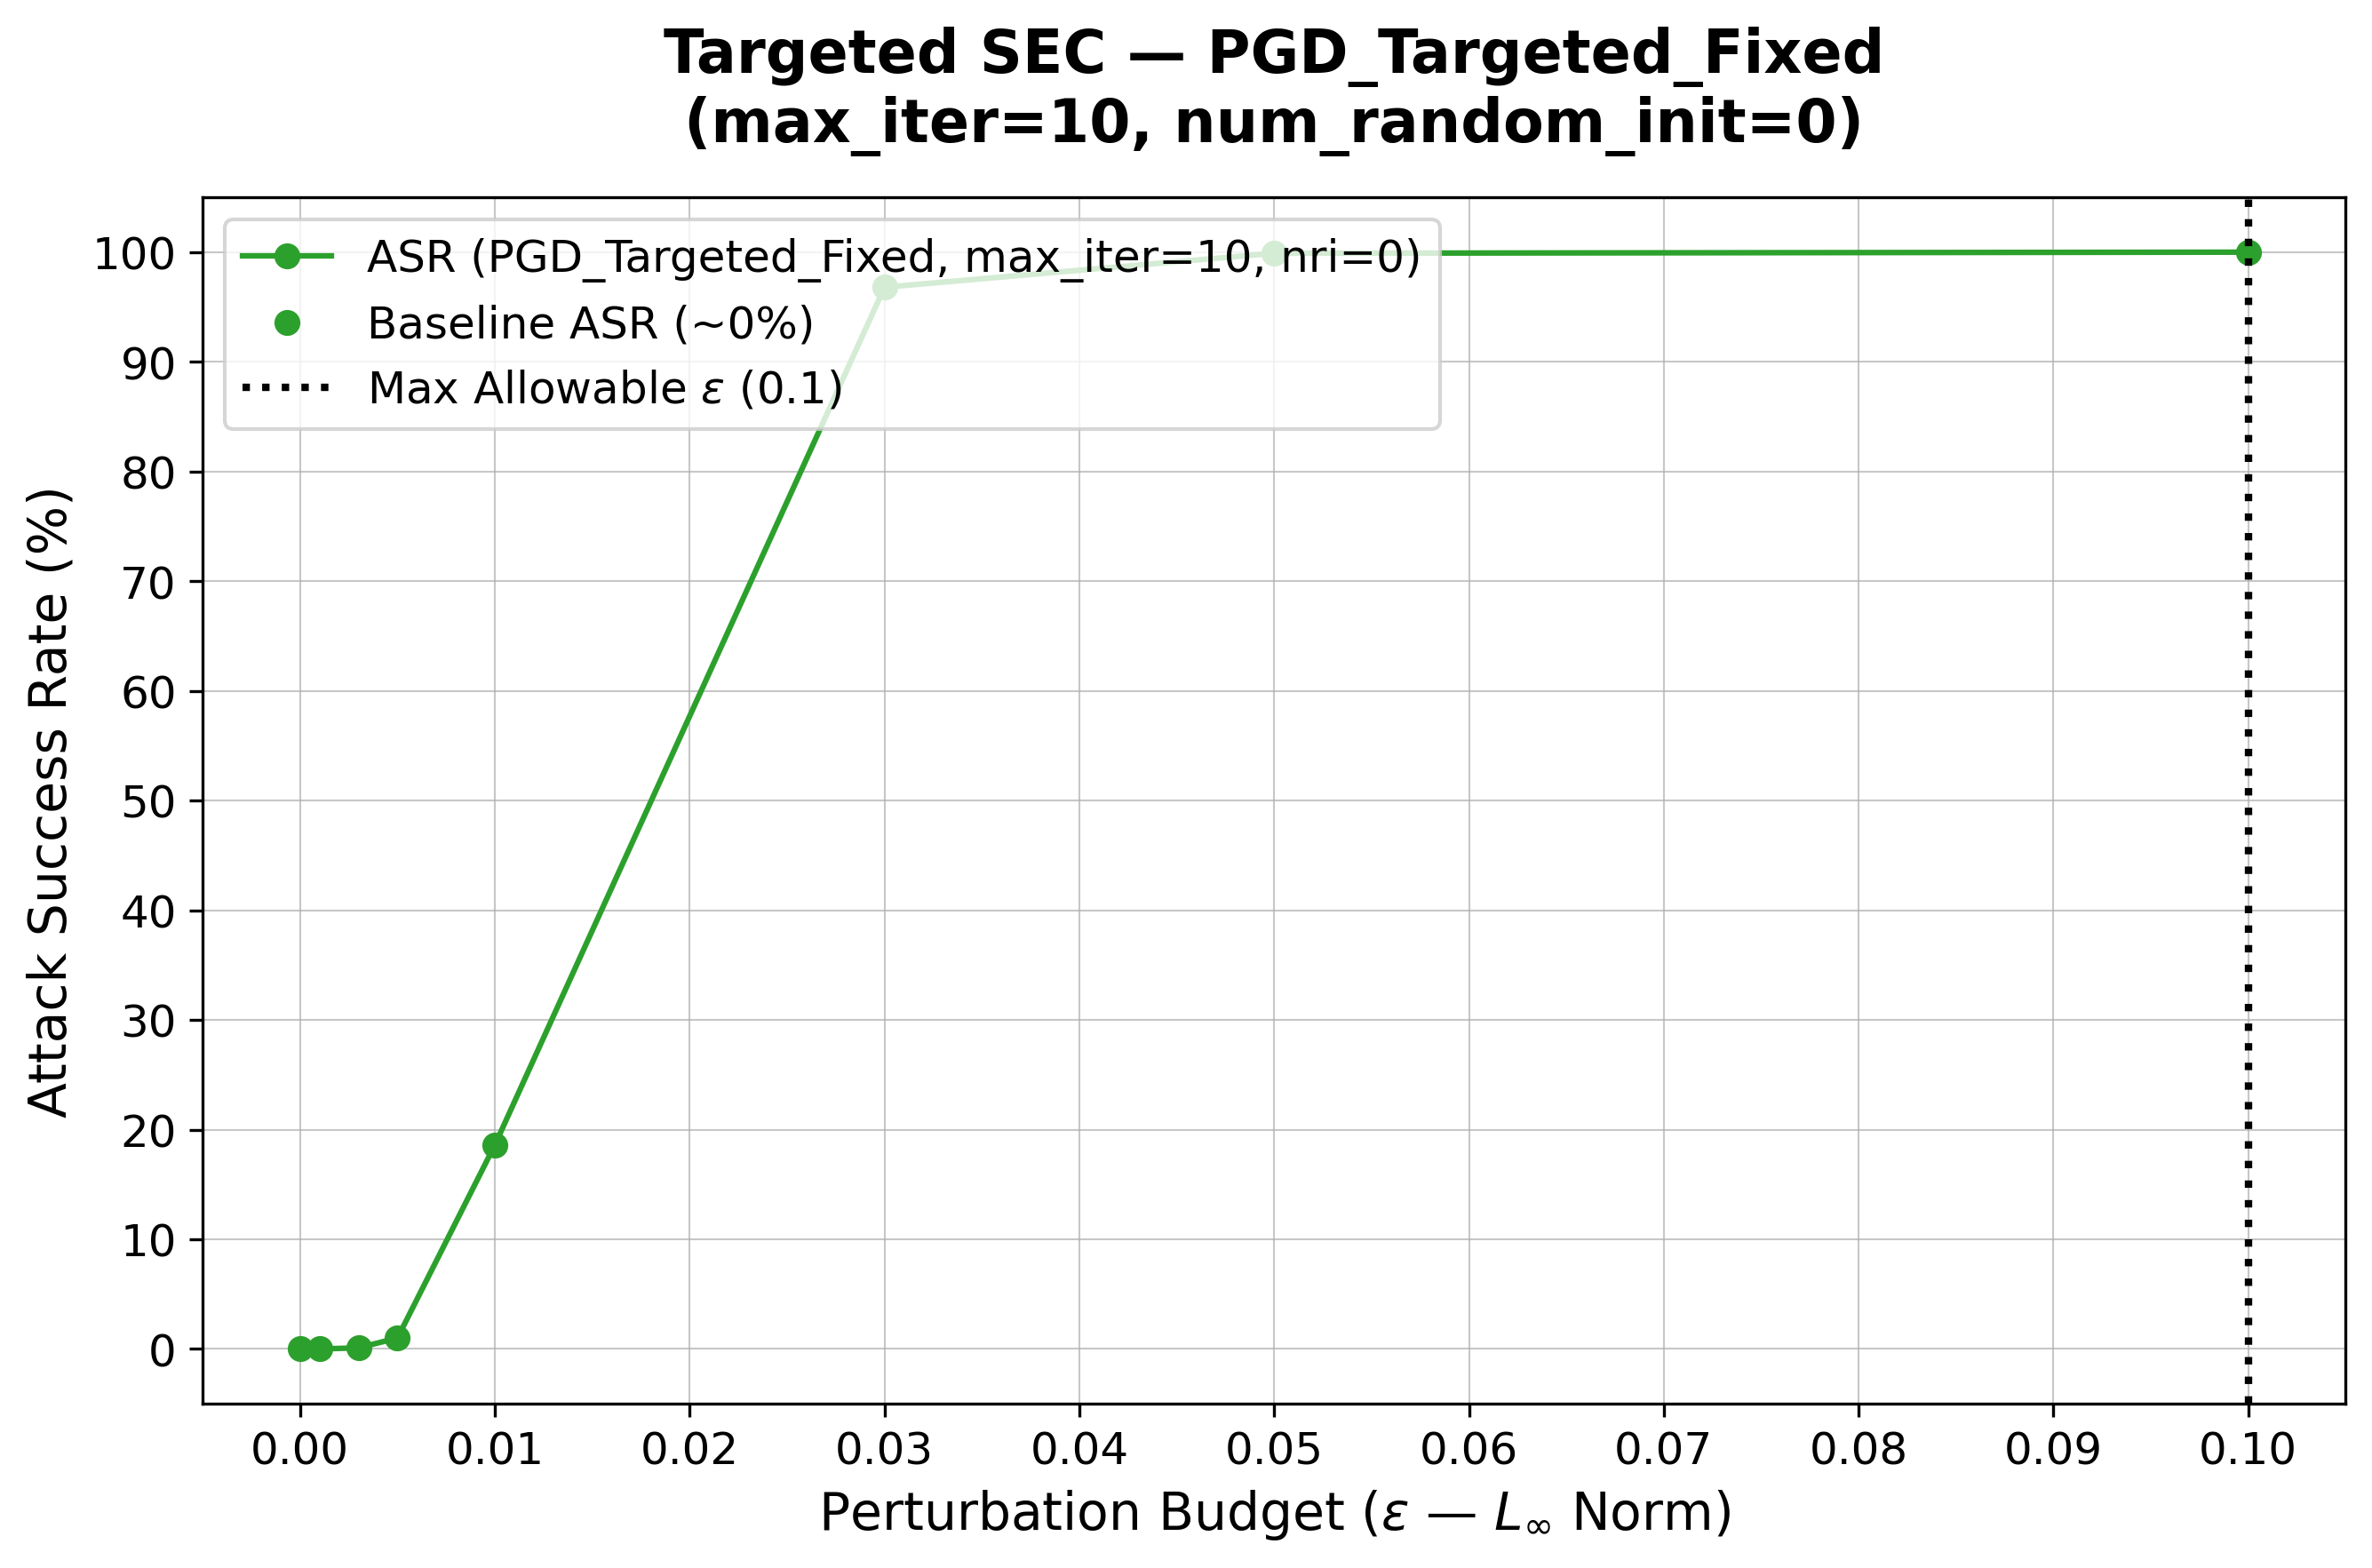
\includegraphics[width=\textwidth]{PGD_Error_specific/Fixed/PGD_Targeted_Fixed_nri0_iter10_SEC.png}
        \caption{\texttt{max_iter} = 10}
        \label{fig:PGD_iter10}
    \end{subfigure}
    \hfill
    % Sotto-figura 4
    \begin{subfigure}[b]{0.45\textwidth}
        \centering
        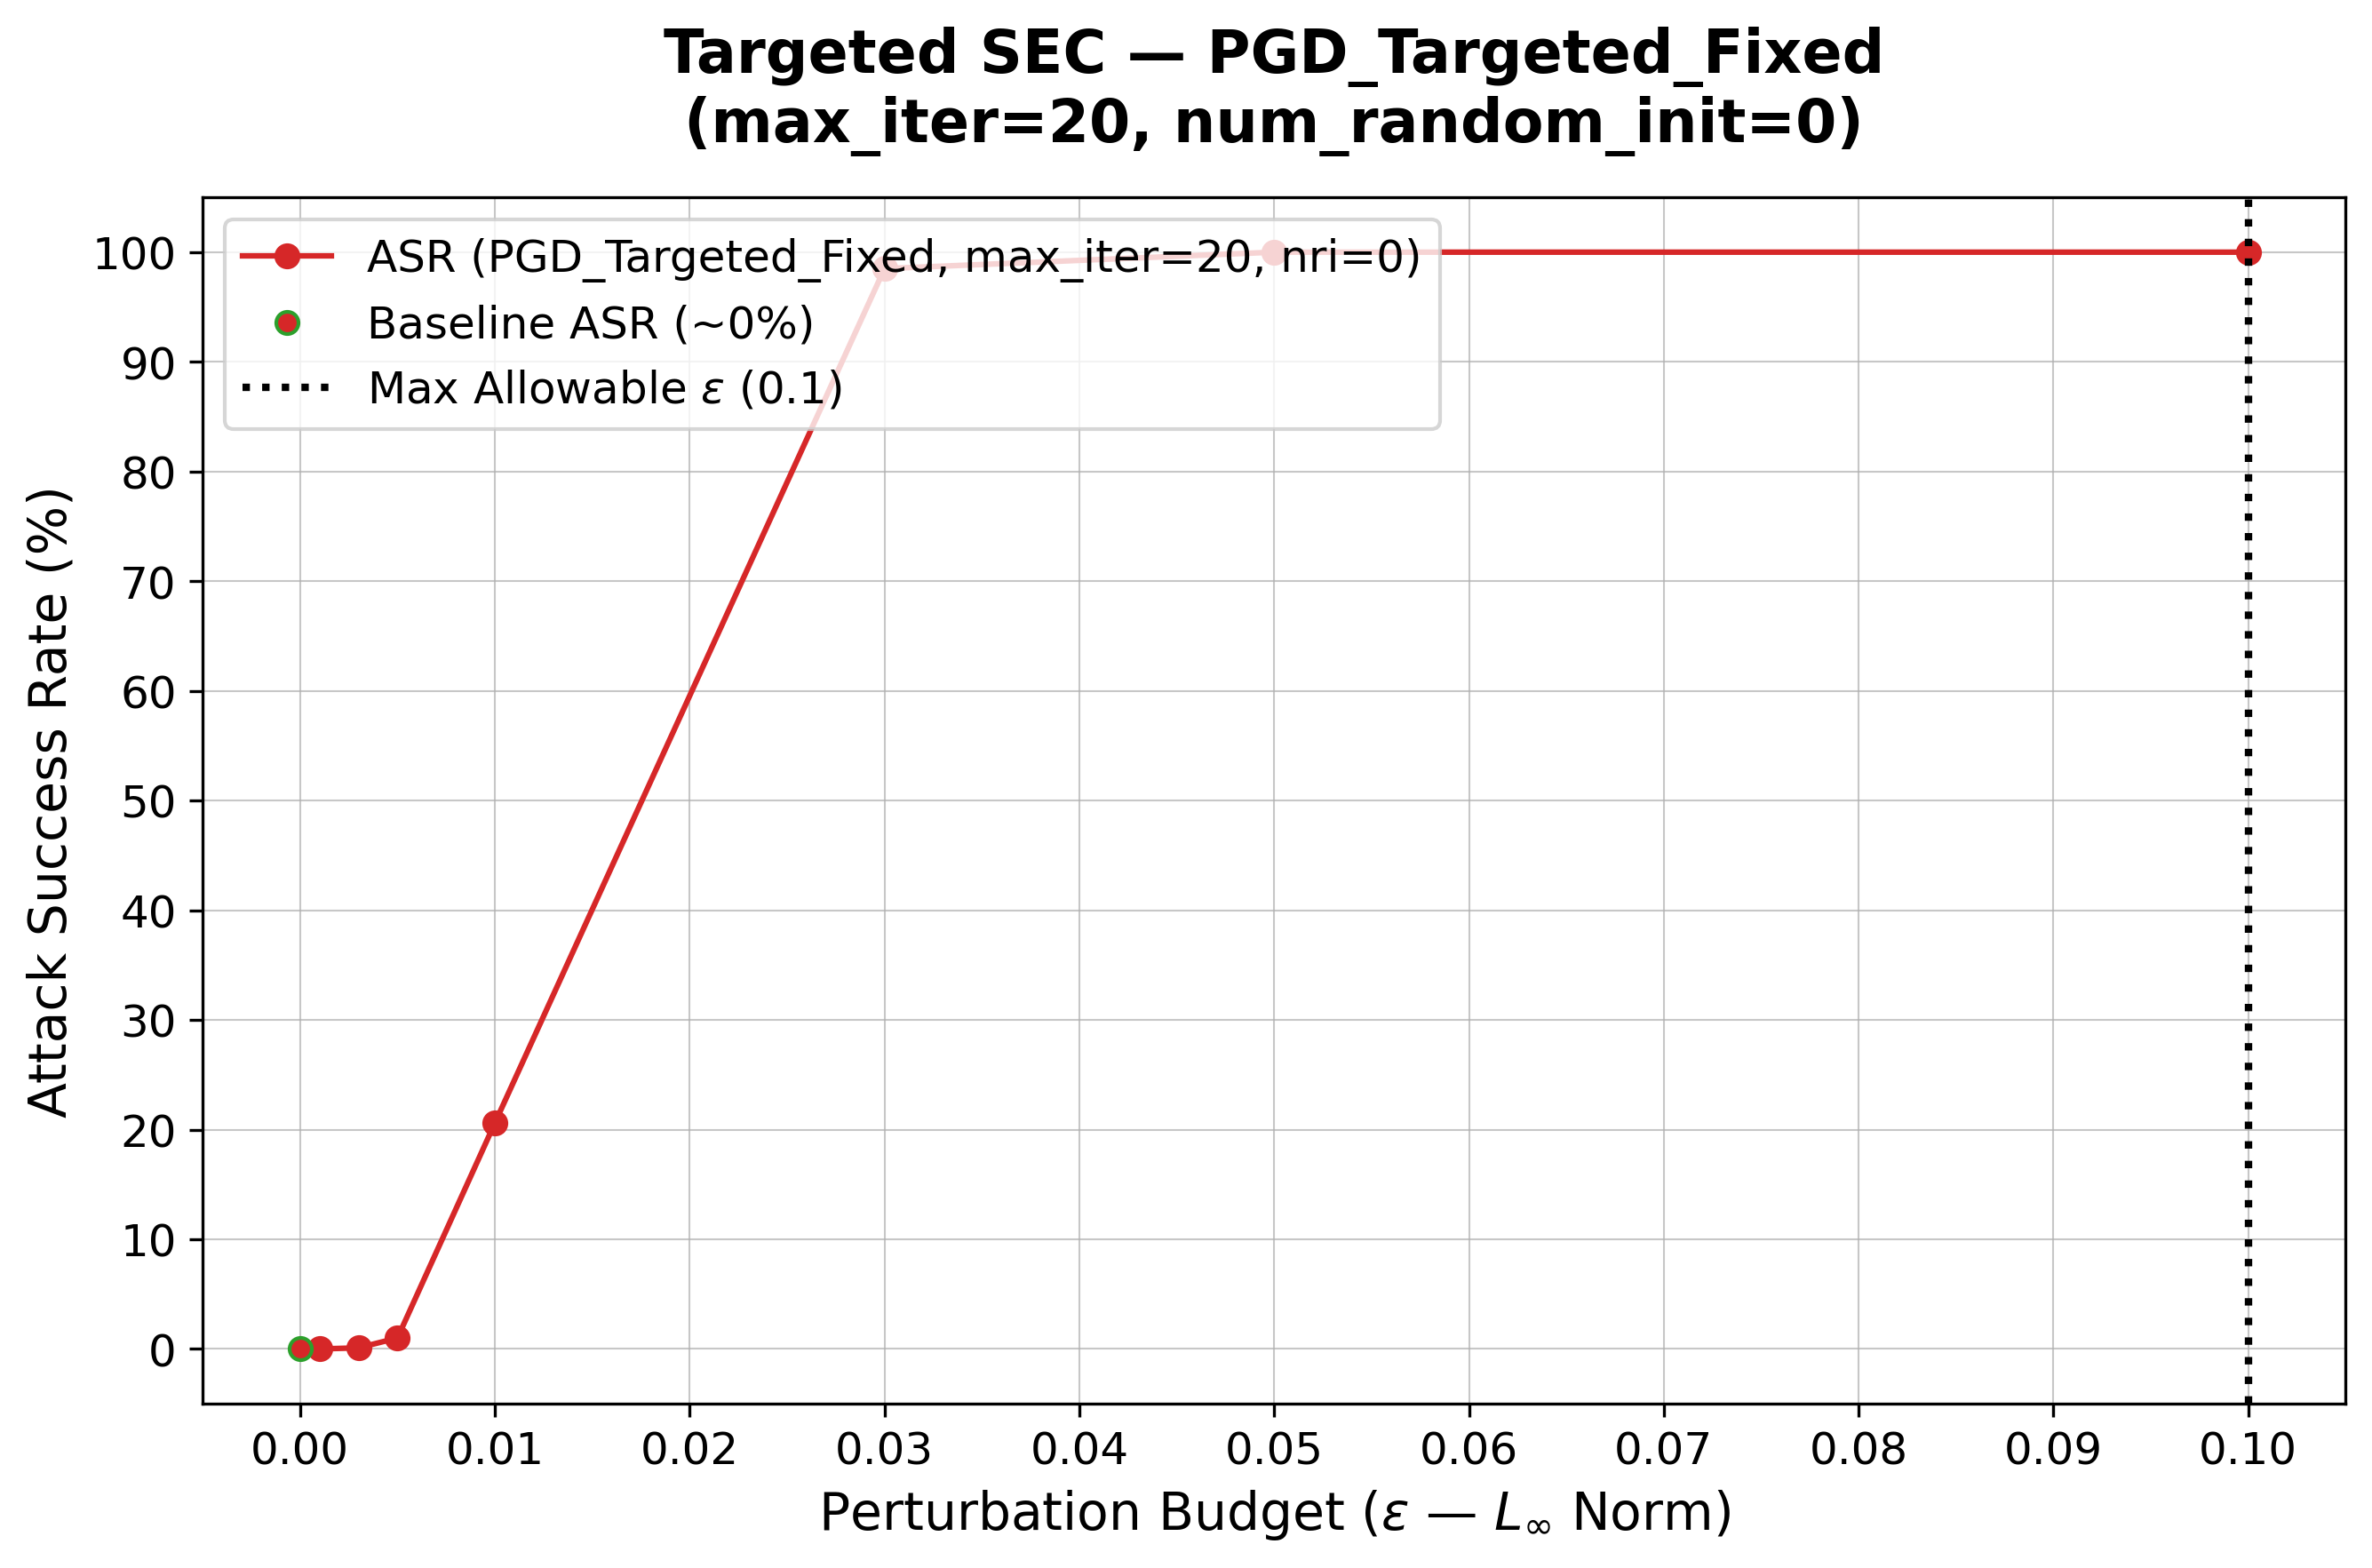
\includegraphics[width=\textwidth]{PGD_Error_specific/Fixed/PGD_Targeted_Fixed_nri0_iter20_SEC.png}
        \caption{\texttt{max_iter} = 20}
        \label{fig:PGD_iter20}
    \end{subfigure}
    \vspace{1em} % Spazio verticale tra le righe di immagini

    % Sotto-figura 5
    \begin{subfigure}[b]{0.45\textwidth}
        \centering
        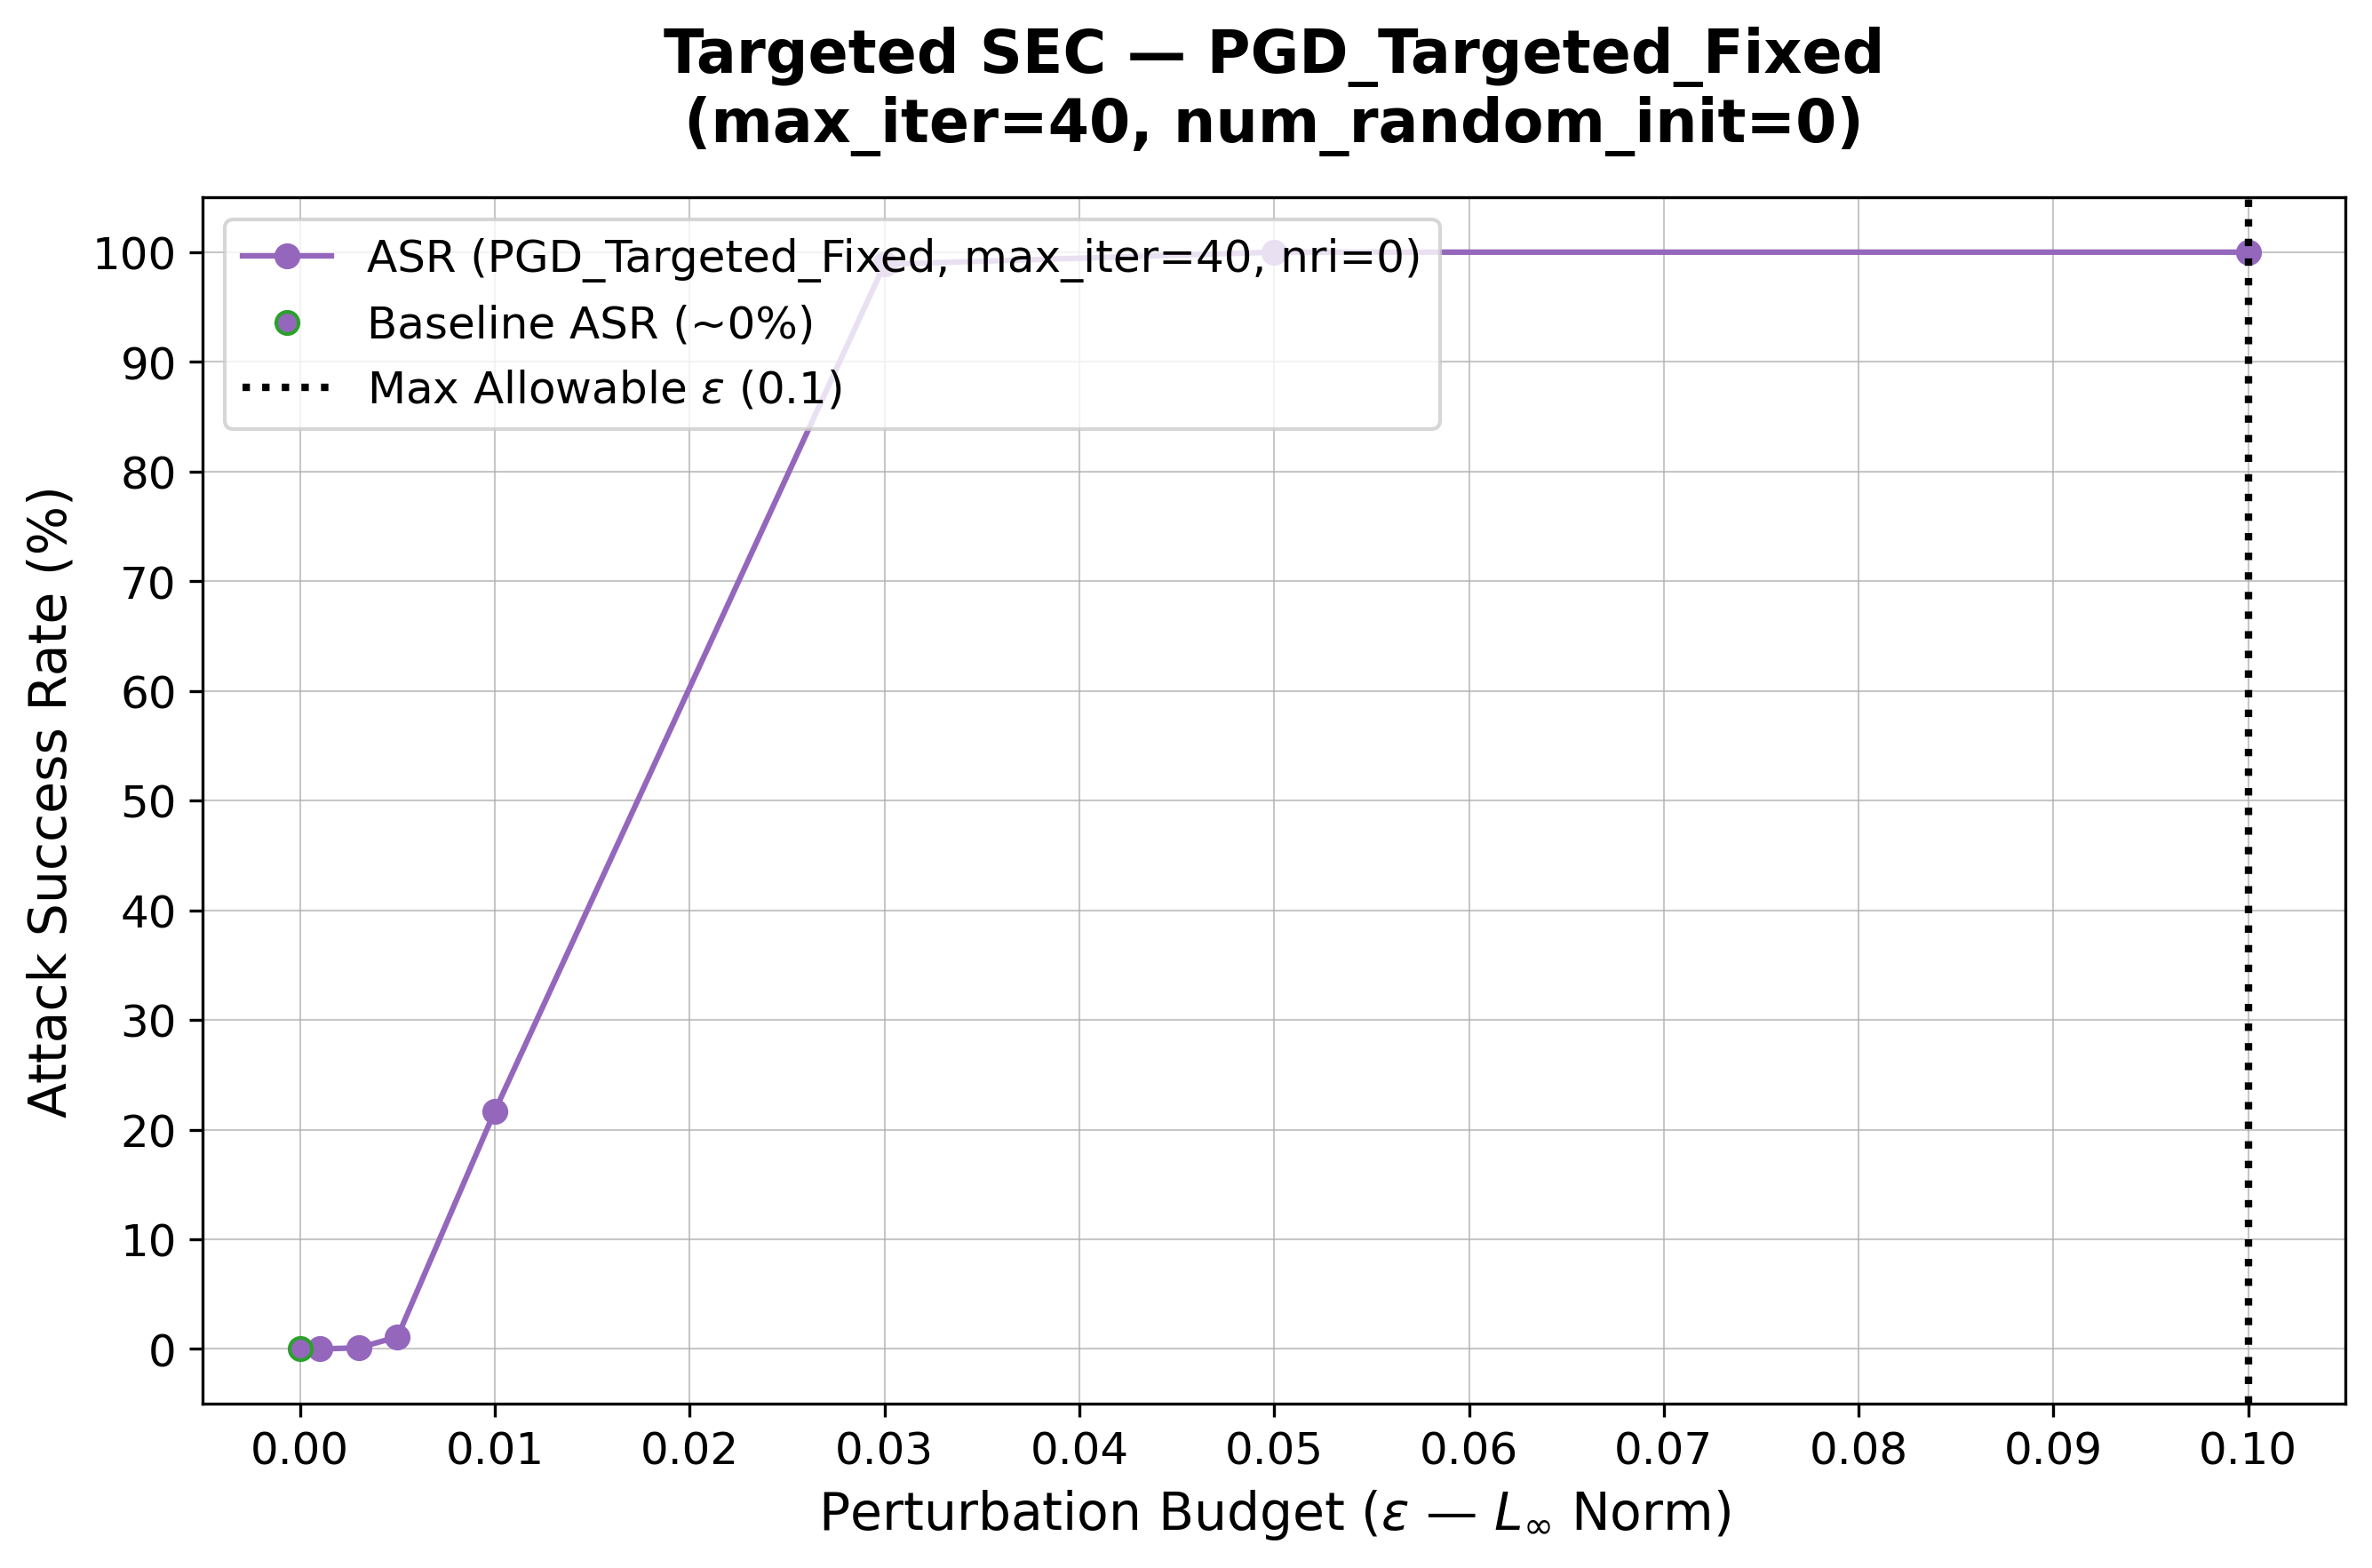
\includegraphics[width=\textwidth]{PGD_Error_specific/Fixed/PGD_Targeted_Fixed_nri0_iter40_SEC.png}
        \caption{\texttt{max_iter} = 40}
        \label{fig:PGD_iter40}
    \end{subfigure}

    \caption{PGD - Iterazioni a confronto per \texttt{nri} = 0}
    \label{fig:PGD_iterations}
\end{figure}

% -- SEC NRI = 1 -- 
\begin{figure}[H]
    \centering
    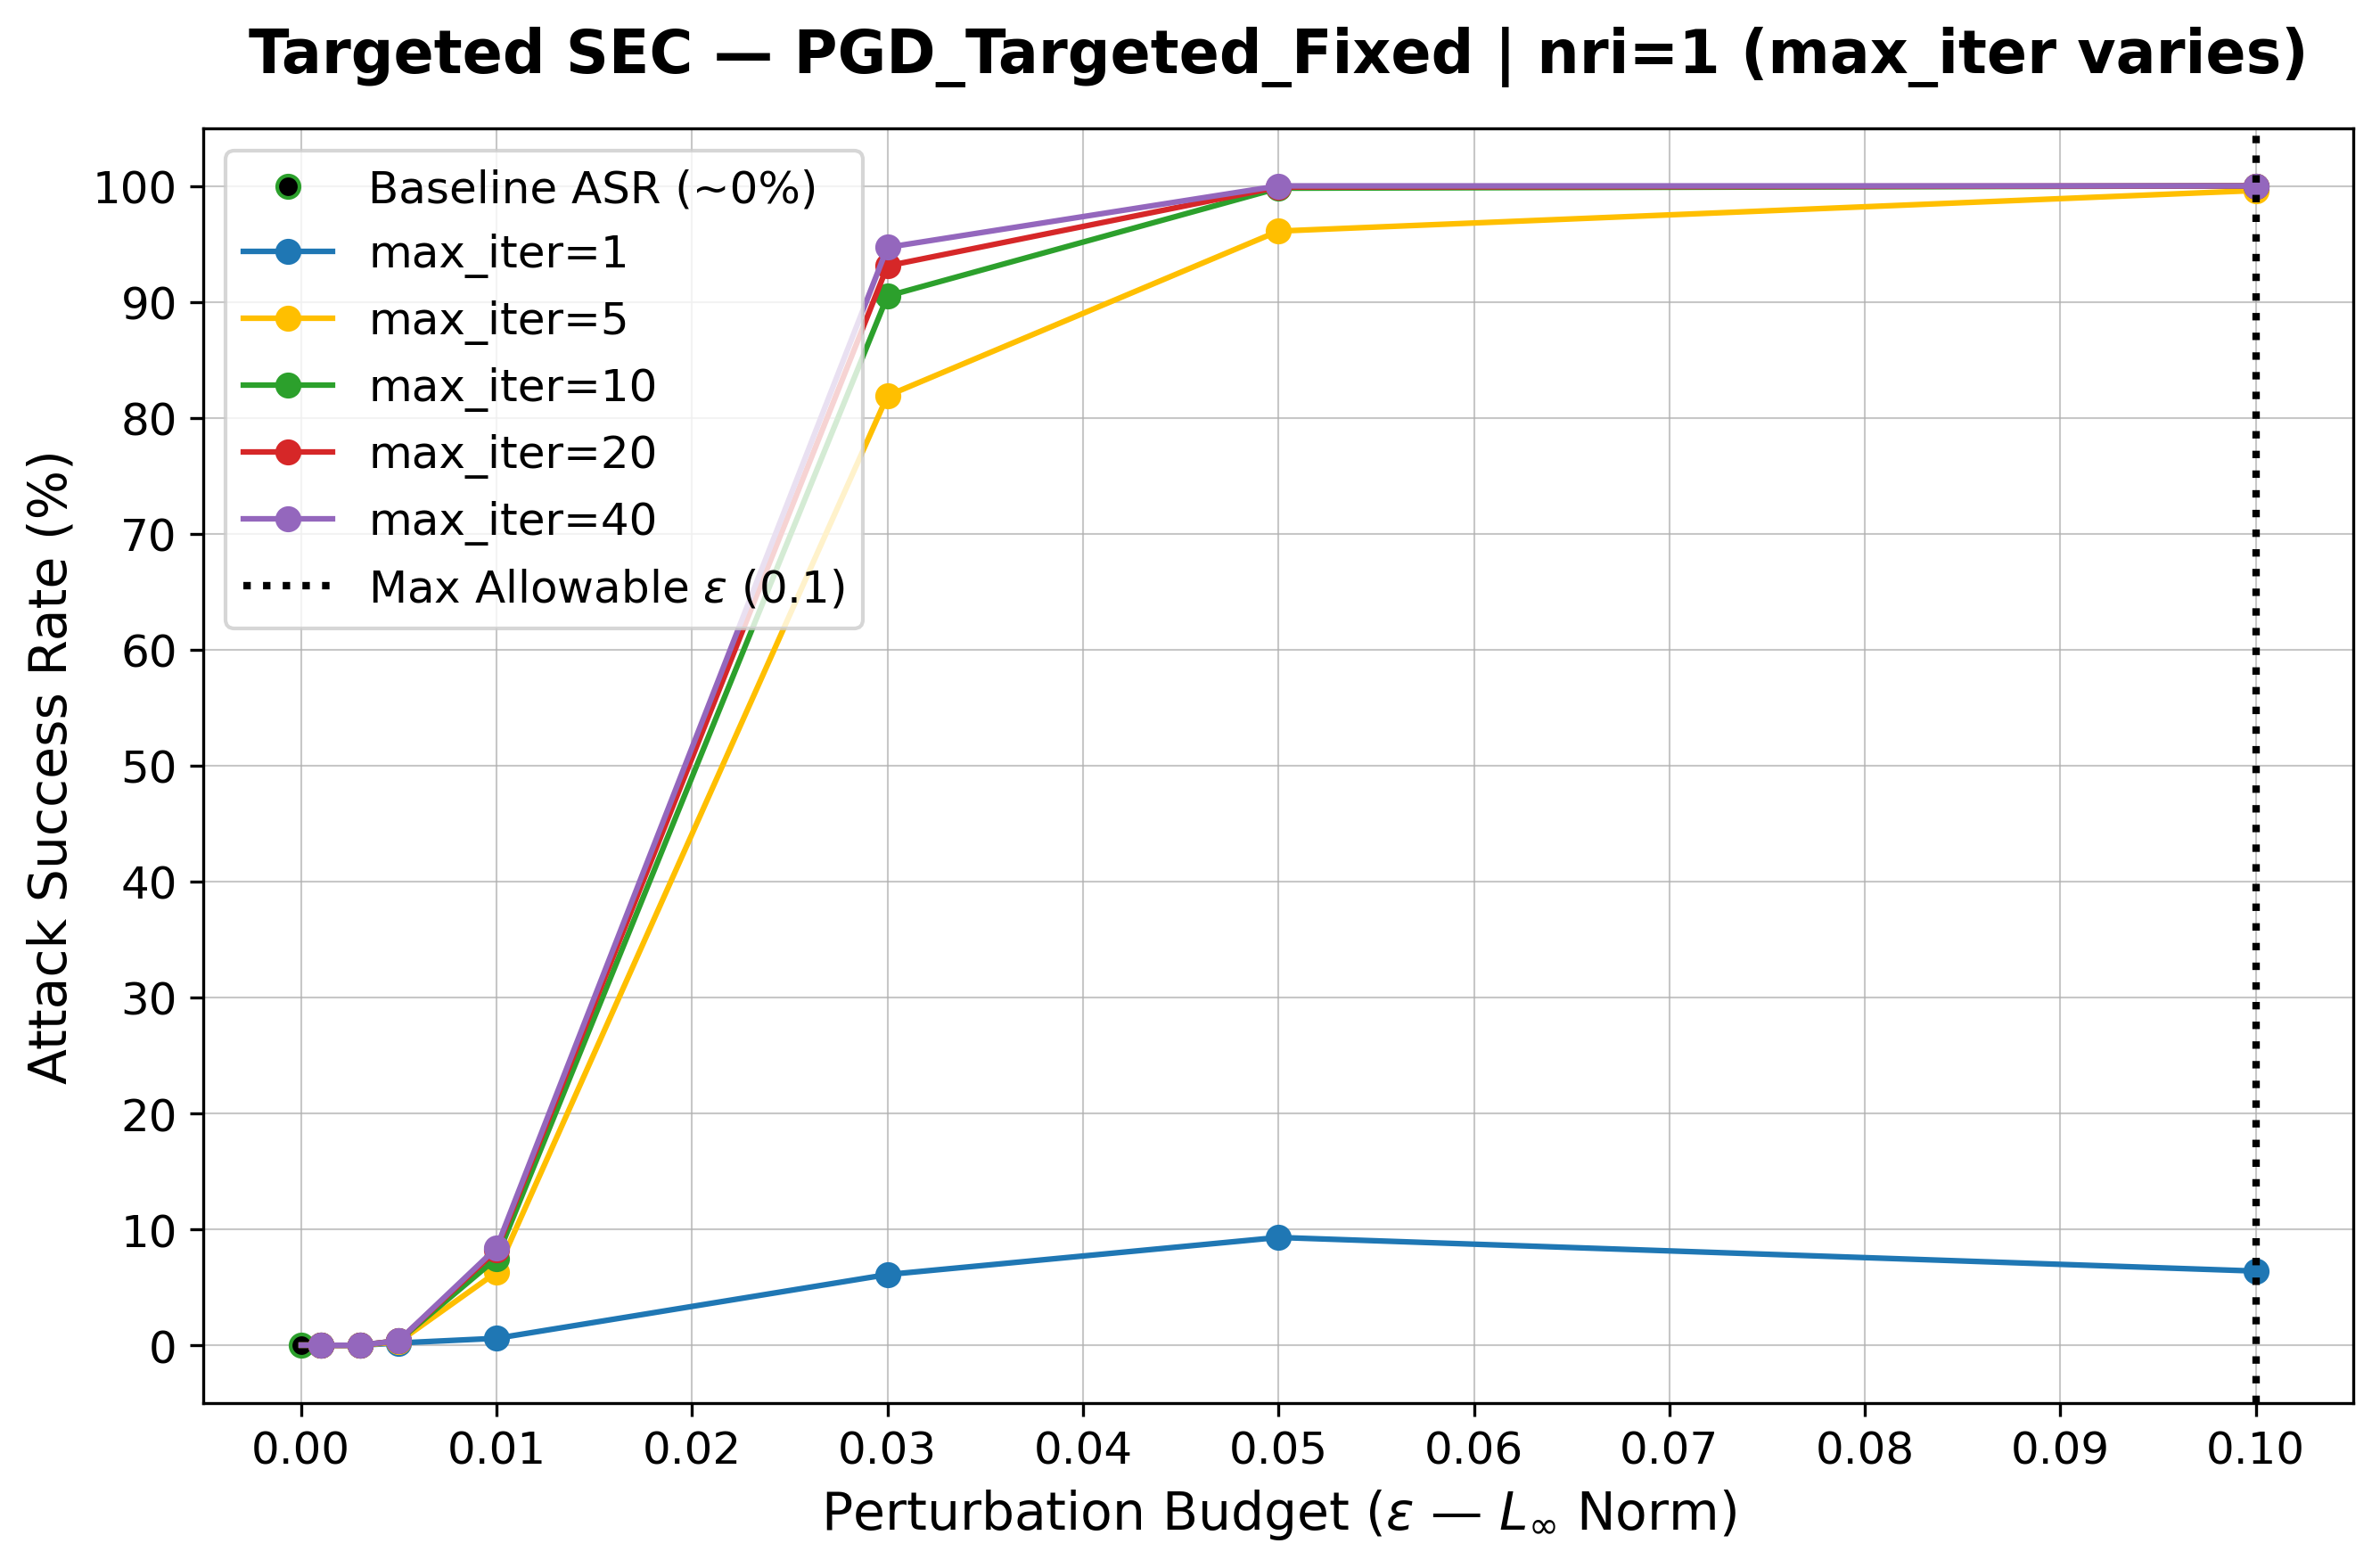
\includegraphics[width=0.5\linewidth]{PGD_Error_specific/Fixed/PGD_Targeted_Fixed_nri1_comparative_maxiter_SEC.png}
    \caption{PGD SEC con nri = 1}
    \label{fig:PGD_SEC_nri1}
\end{figure}

% -- SOTTO GRAFICI PER NRI = 1
\begin{figure}[H]
    \centering
    % Sotto-figura 1
    \begin{subfigure}[b]{0.45\textwidth}
        \centering
        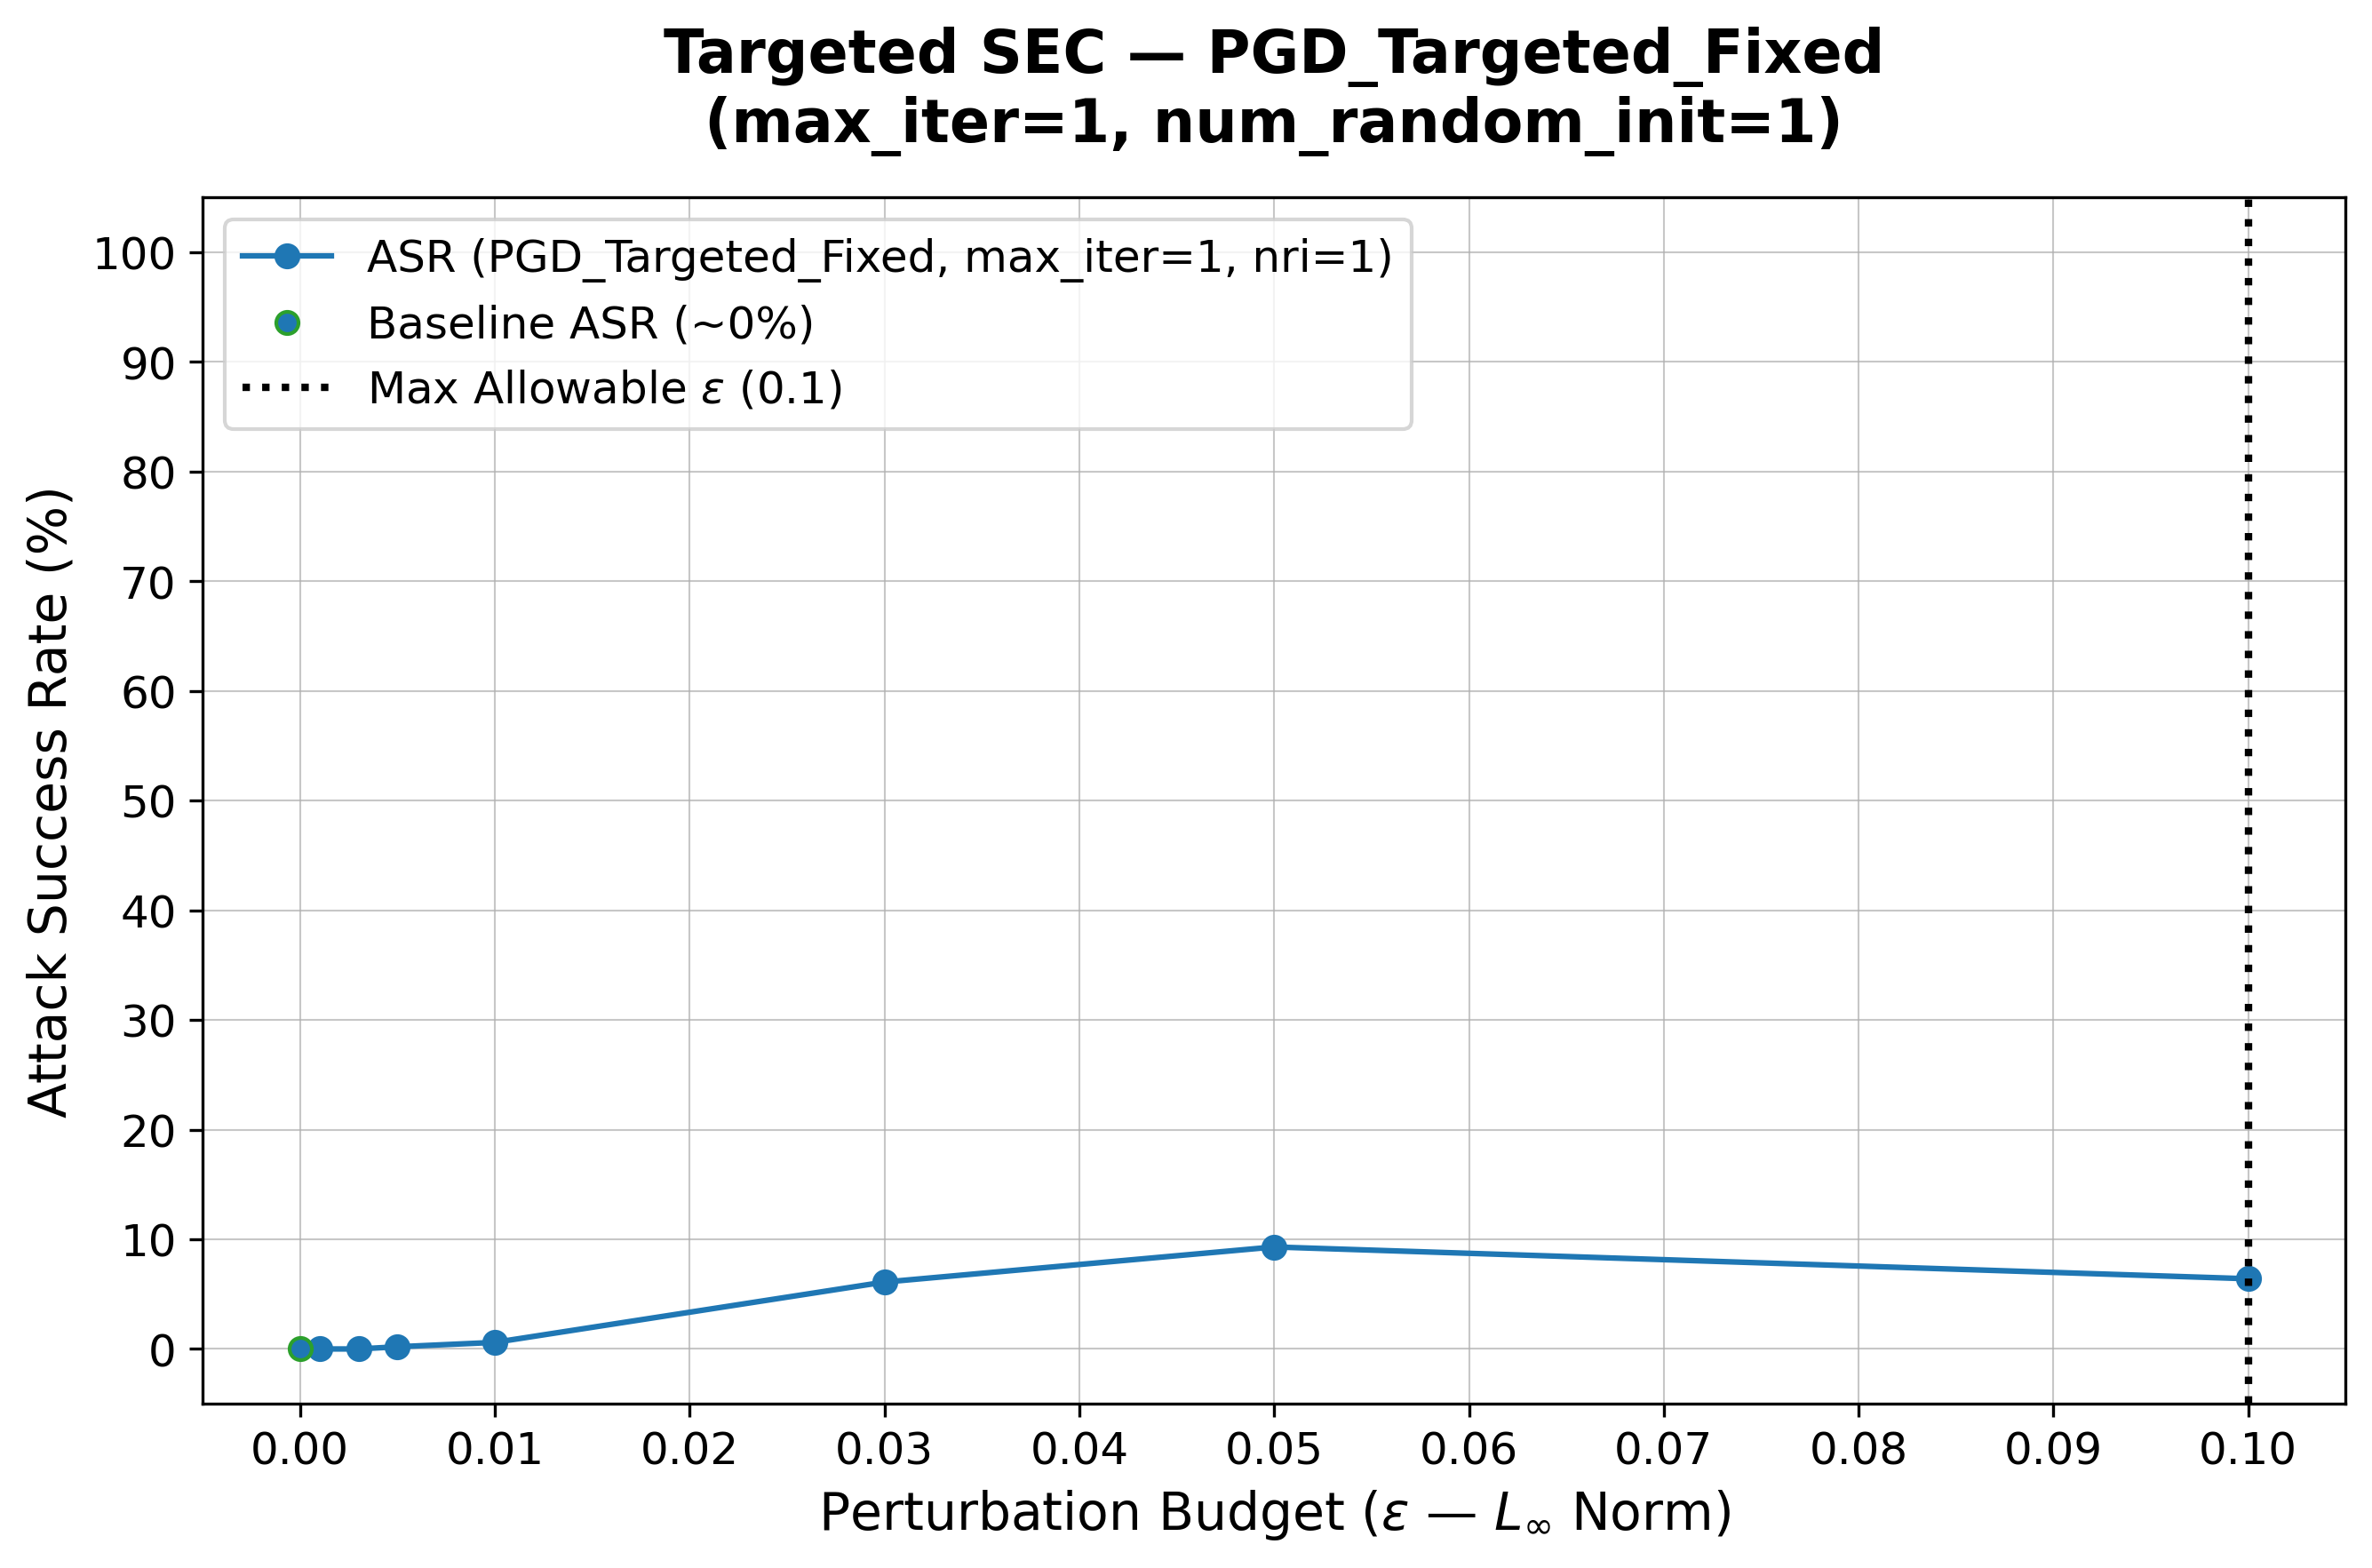
\includegraphics[width=\textwidth]{PGD_Error_specific/Fixed/PGD_Targeted_Fixed_nri1_iter1_SEC.png}
        \caption{\texttt{max_iter} = 1}
        \label{fig:PGD_nri1_iter1}
    \end{subfigure}
    \hfill
    % Sotto-figura 2
    \begin{subfigure}[b]{0.45\textwidth}
        \centering
        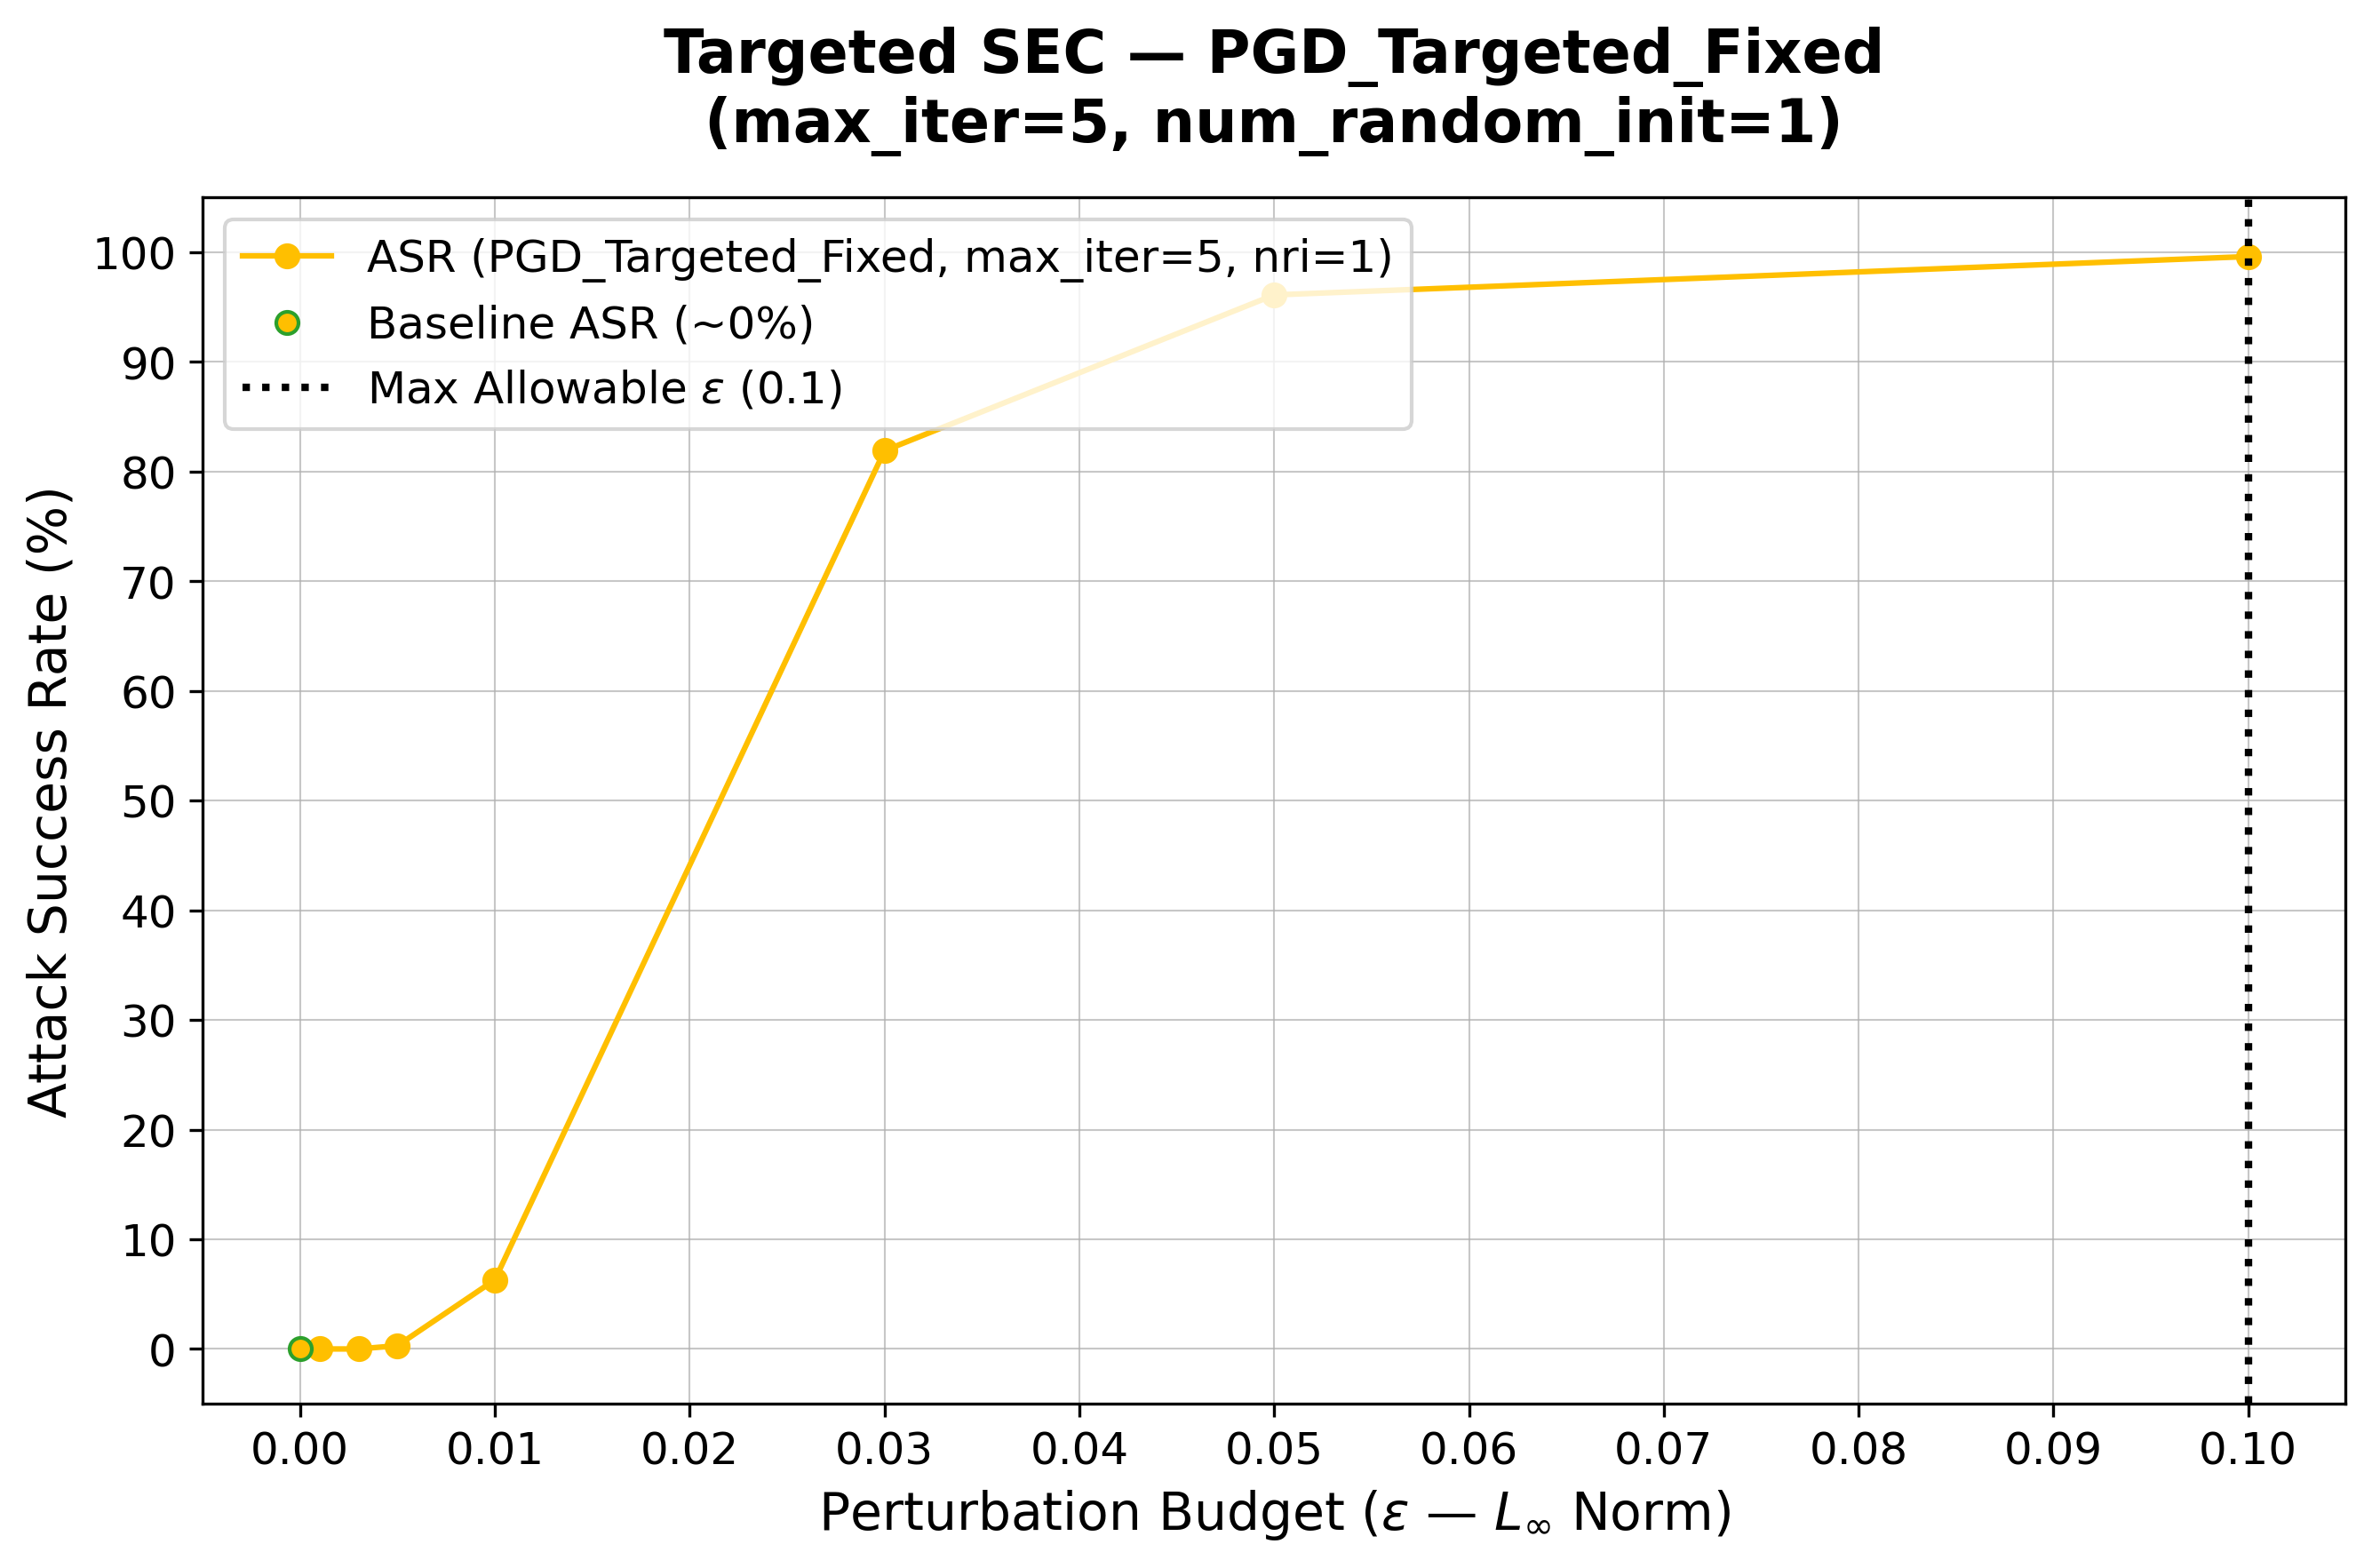
\includegraphics[width=\textwidth]{PGD_Error_specific/Fixed/PGD_Targeted_Fixed_nri1_iter5_SEC.png}
        \caption{\texttt{max_iter} = 5}
        \label{fig:PGD_nri1_iter5}
    \end{subfigure}

    \vspace{1em} % Spazio verticale tra le righe di immagini   
    % Sotto-figura 3
    \begin{subfigure}[b]{0.45\textwidth}
        \centering
        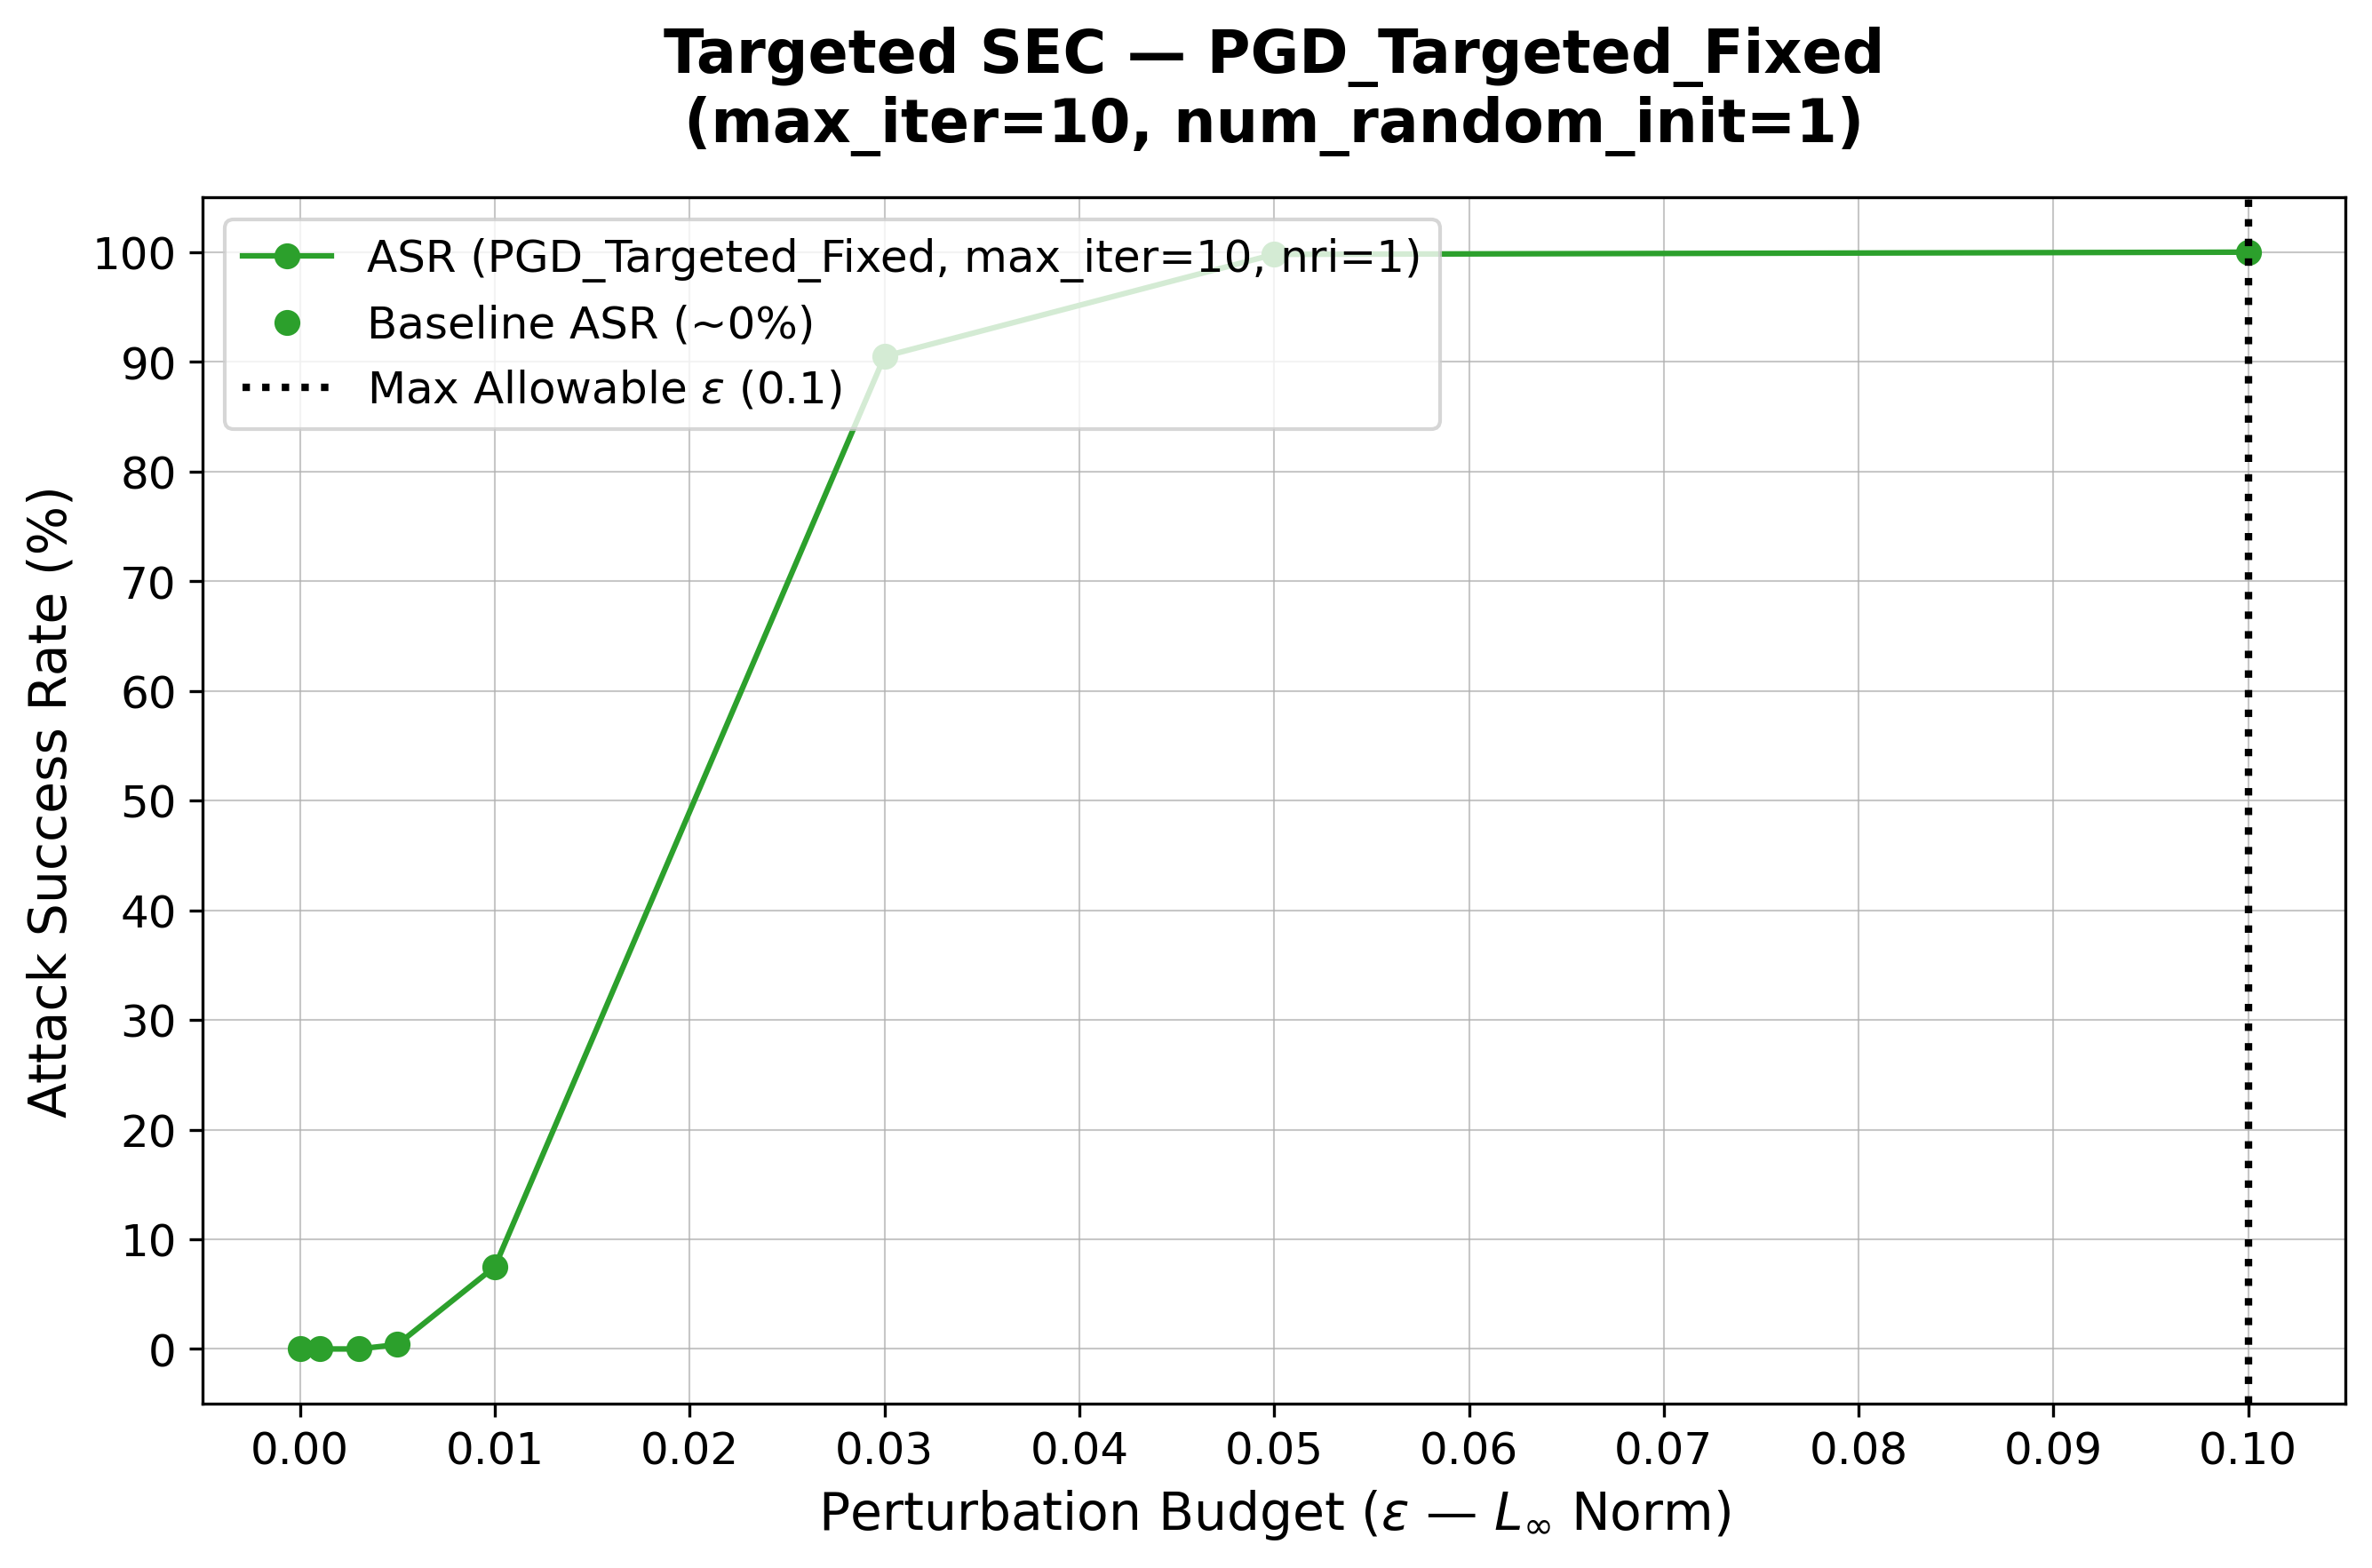
\includegraphics[width=\textwidth]{PGD_Error_specific/Fixed/PGD_Targeted_Fixed_nri1_iter10_SEC.png}
        \caption{\texttt{max_iter} = 10}
        \label{fig:PGD_nri1_iter10}
    \end{subfigure}
    \hfill
    % Sotto-figura 4
    \begin{subfigure}[b]{0.45\textwidth}
        \centering
        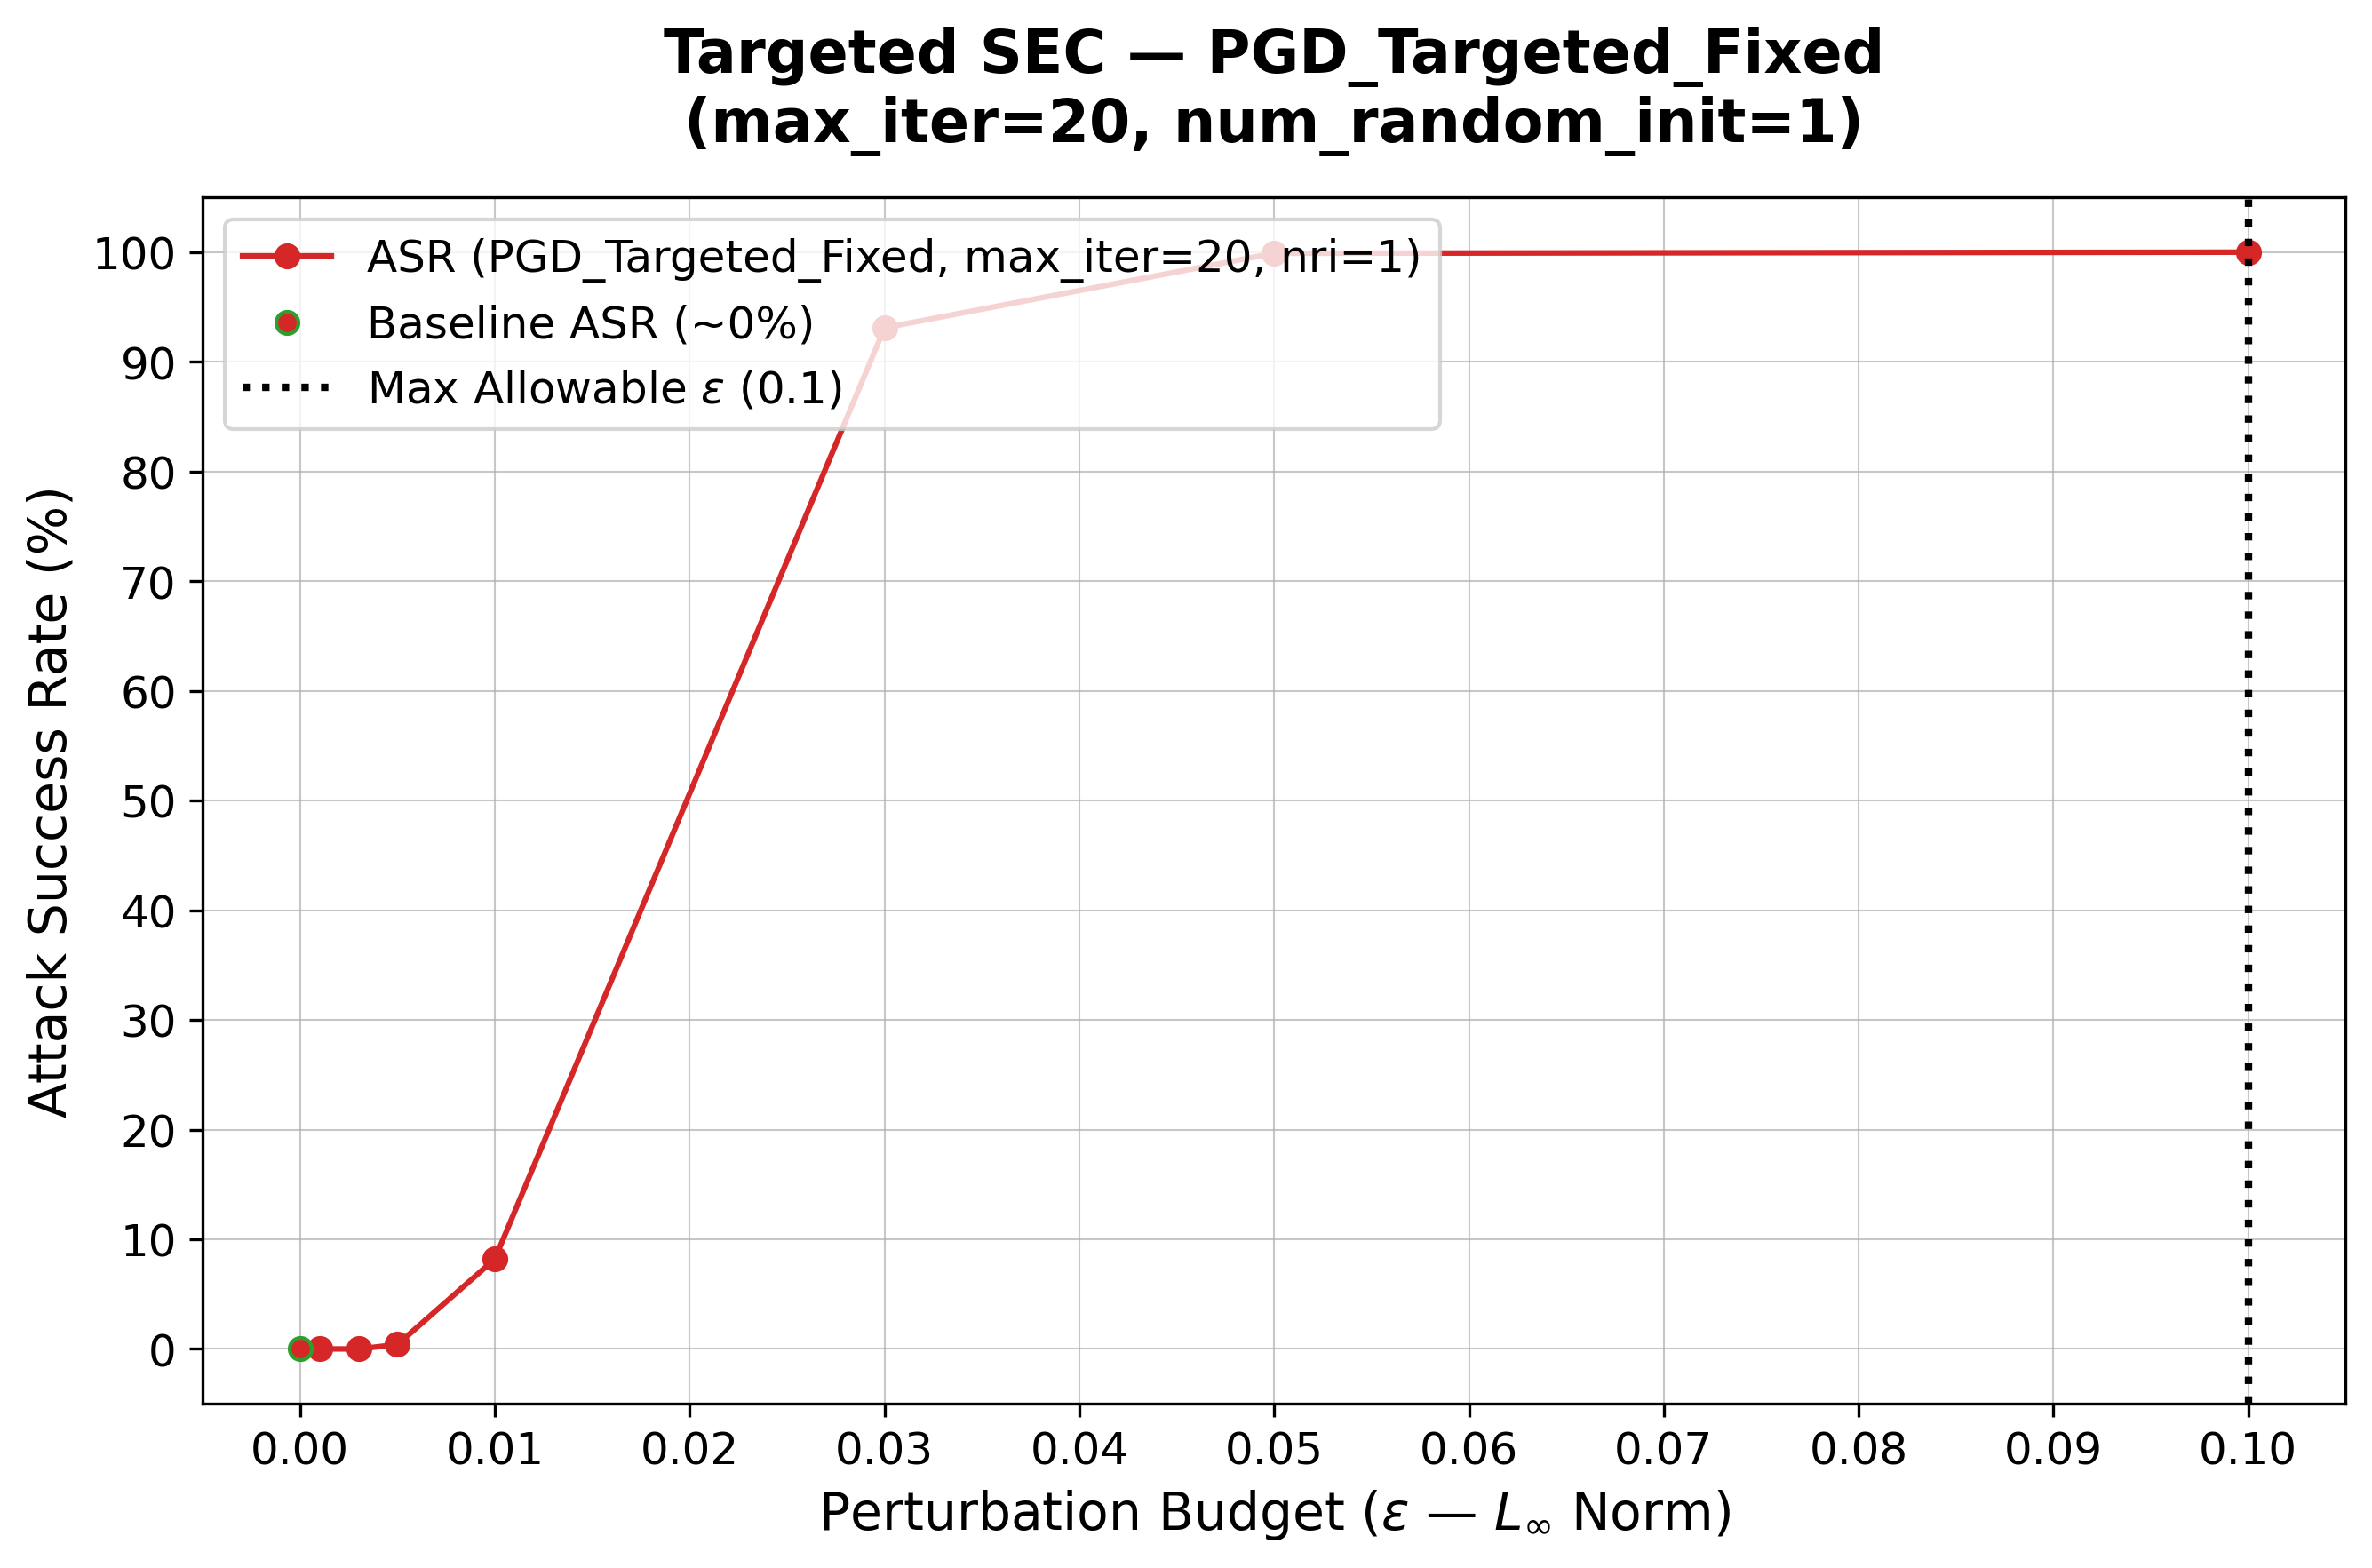
\includegraphics[width=\textwidth]{PGD_Error_specific/Fixed/PGD_Targeted_Fixed_nri1_iter20_SEC.png}
        \caption{\texttt{max_iter} = 20}
        \label{fig:PGD_nri1_iter20}
    \end{subfigure}
    \vspace{1em} % Spazio verticale tra le righe di immagini
    % Sotto-figura 5
    \begin{subfigure}[b]{0.45\textwidth}
        \centering
        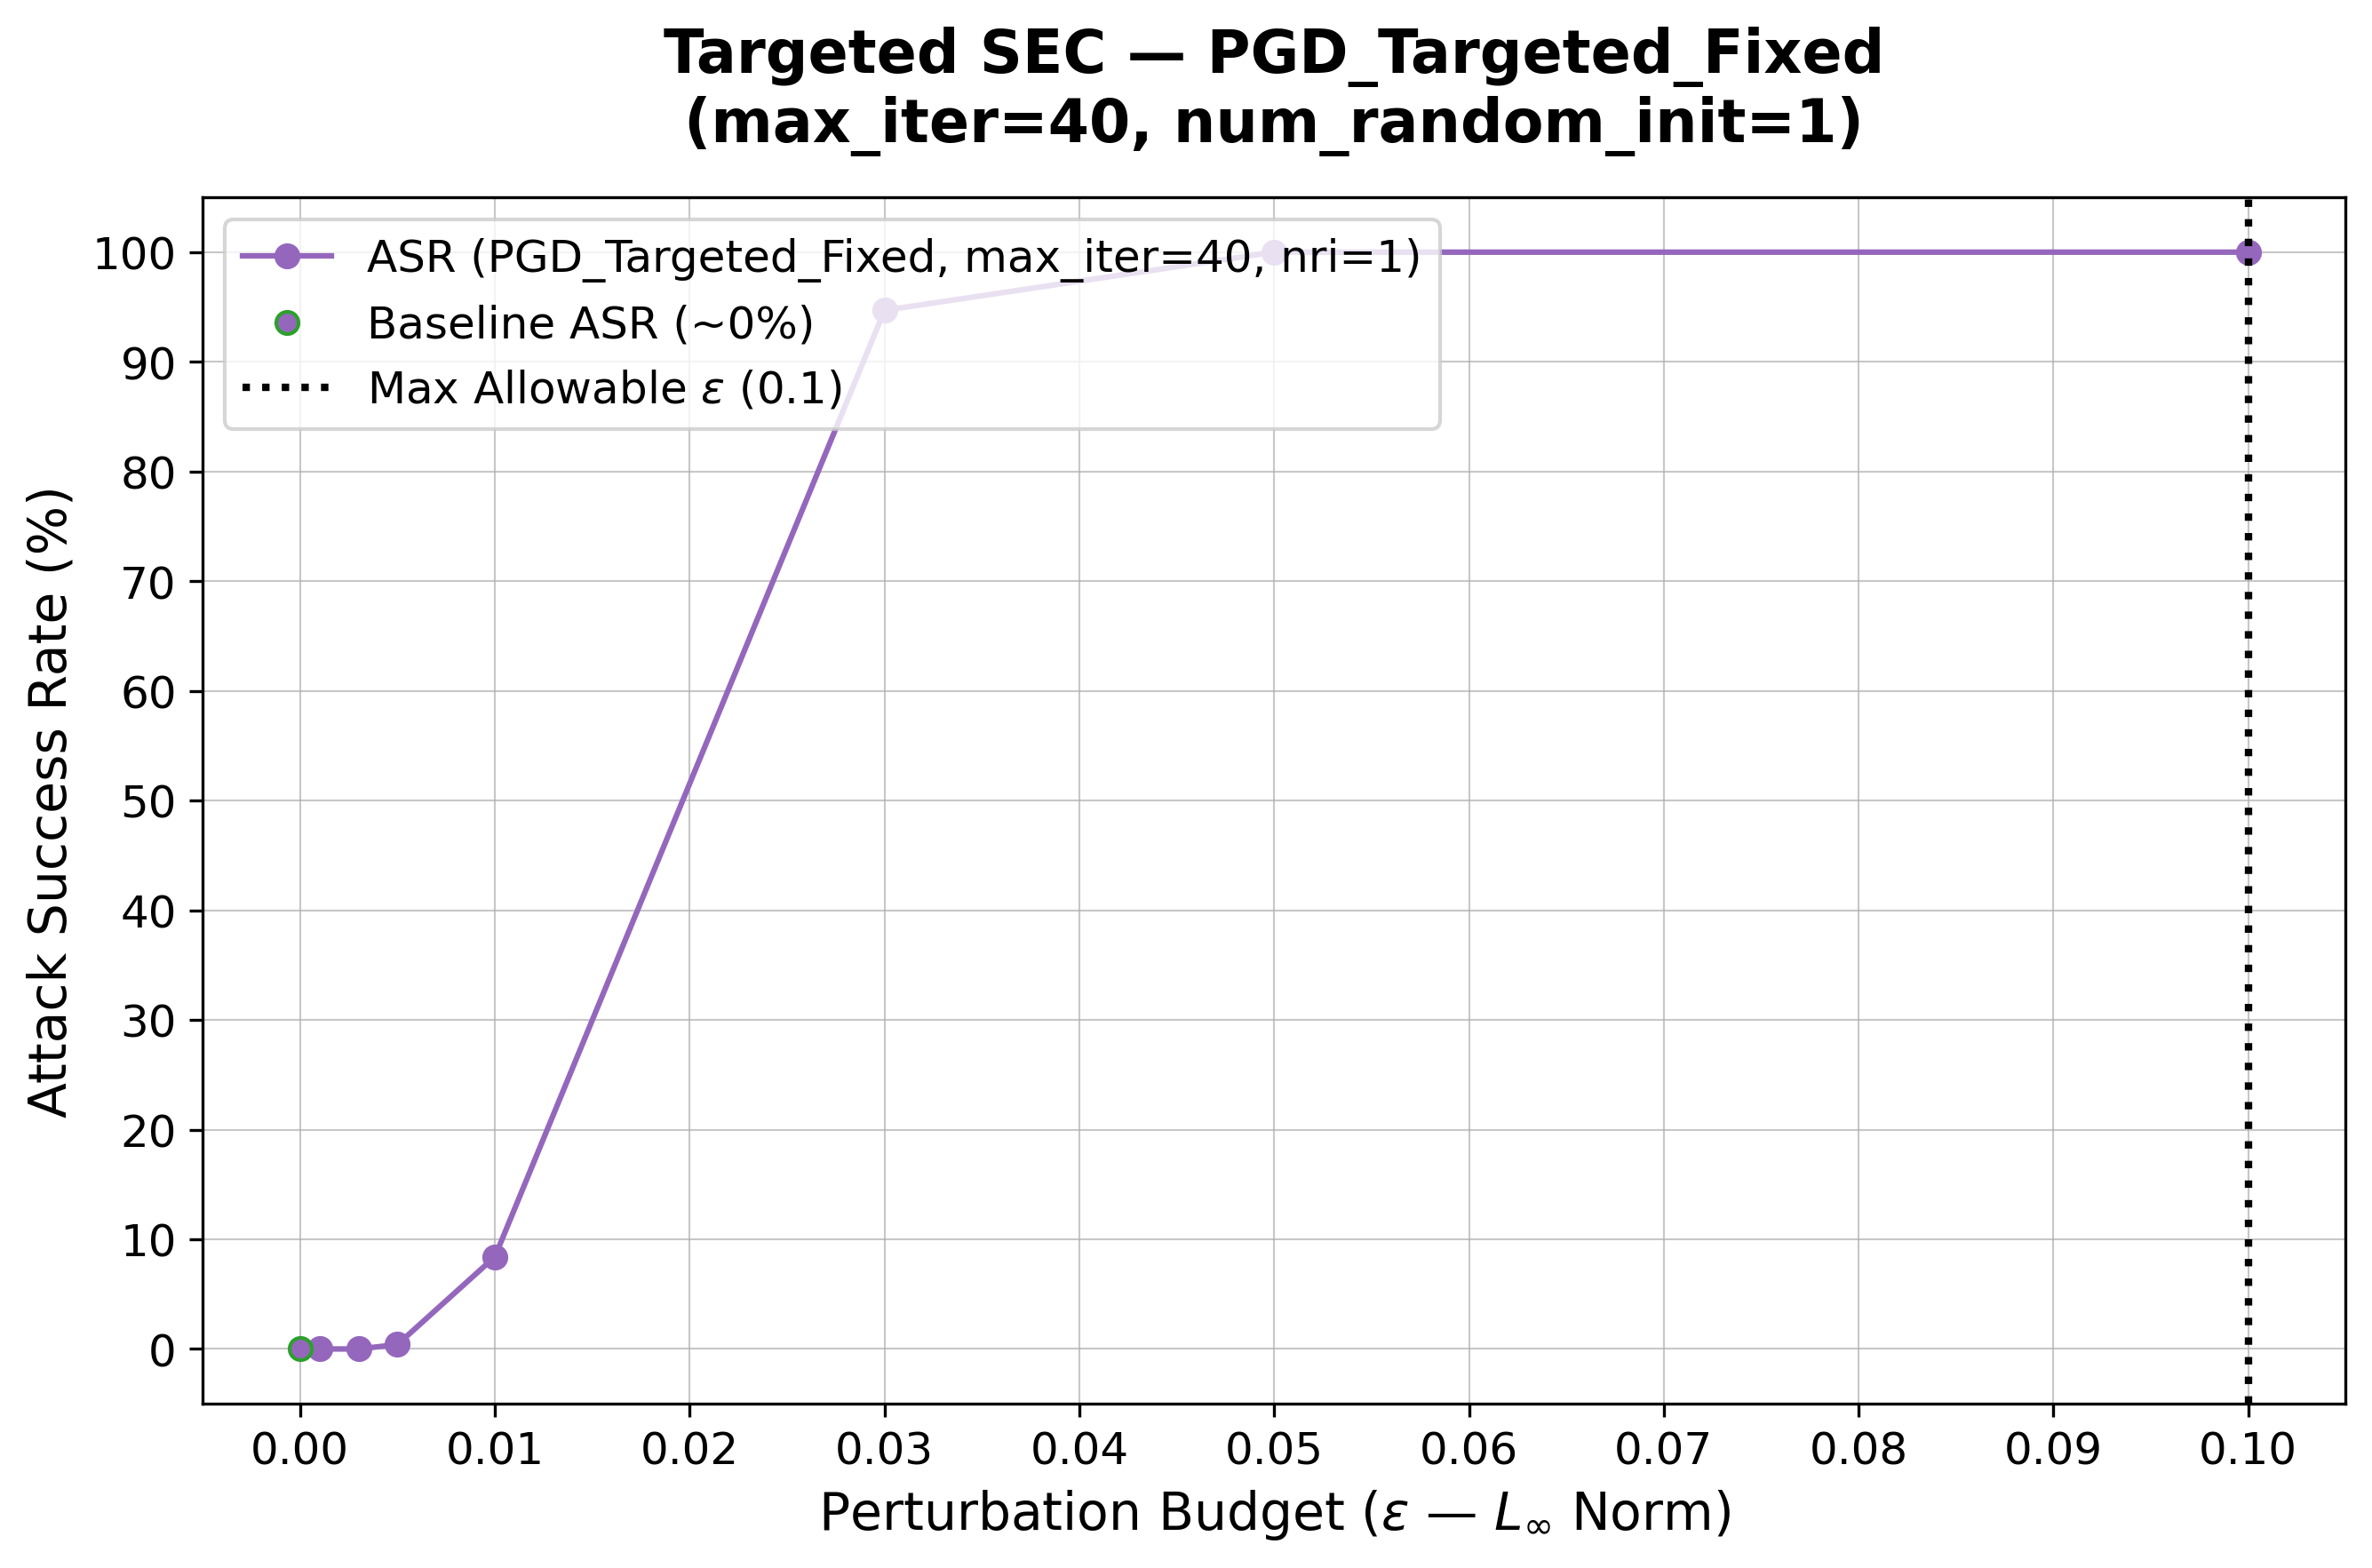
\includegraphics[width=\textwidth]{PGD_Error_specific/Fixed/PGD_Targeted_Fixed_nri1_iter40_SEC.png}
        \caption{\texttt{max_iter} = 40}
        \label{fig:PGD_nri1_iter40}
    \end{subfigure}
    \caption{PGD Fixed - Iterazioni a confronto per \texttt{nri} = 1}
    \label{fig:PGD_iterations_nri1}
\end{figure}

% -- SEC NRI = 3 --
\begin{figure}[H]
    \centering
    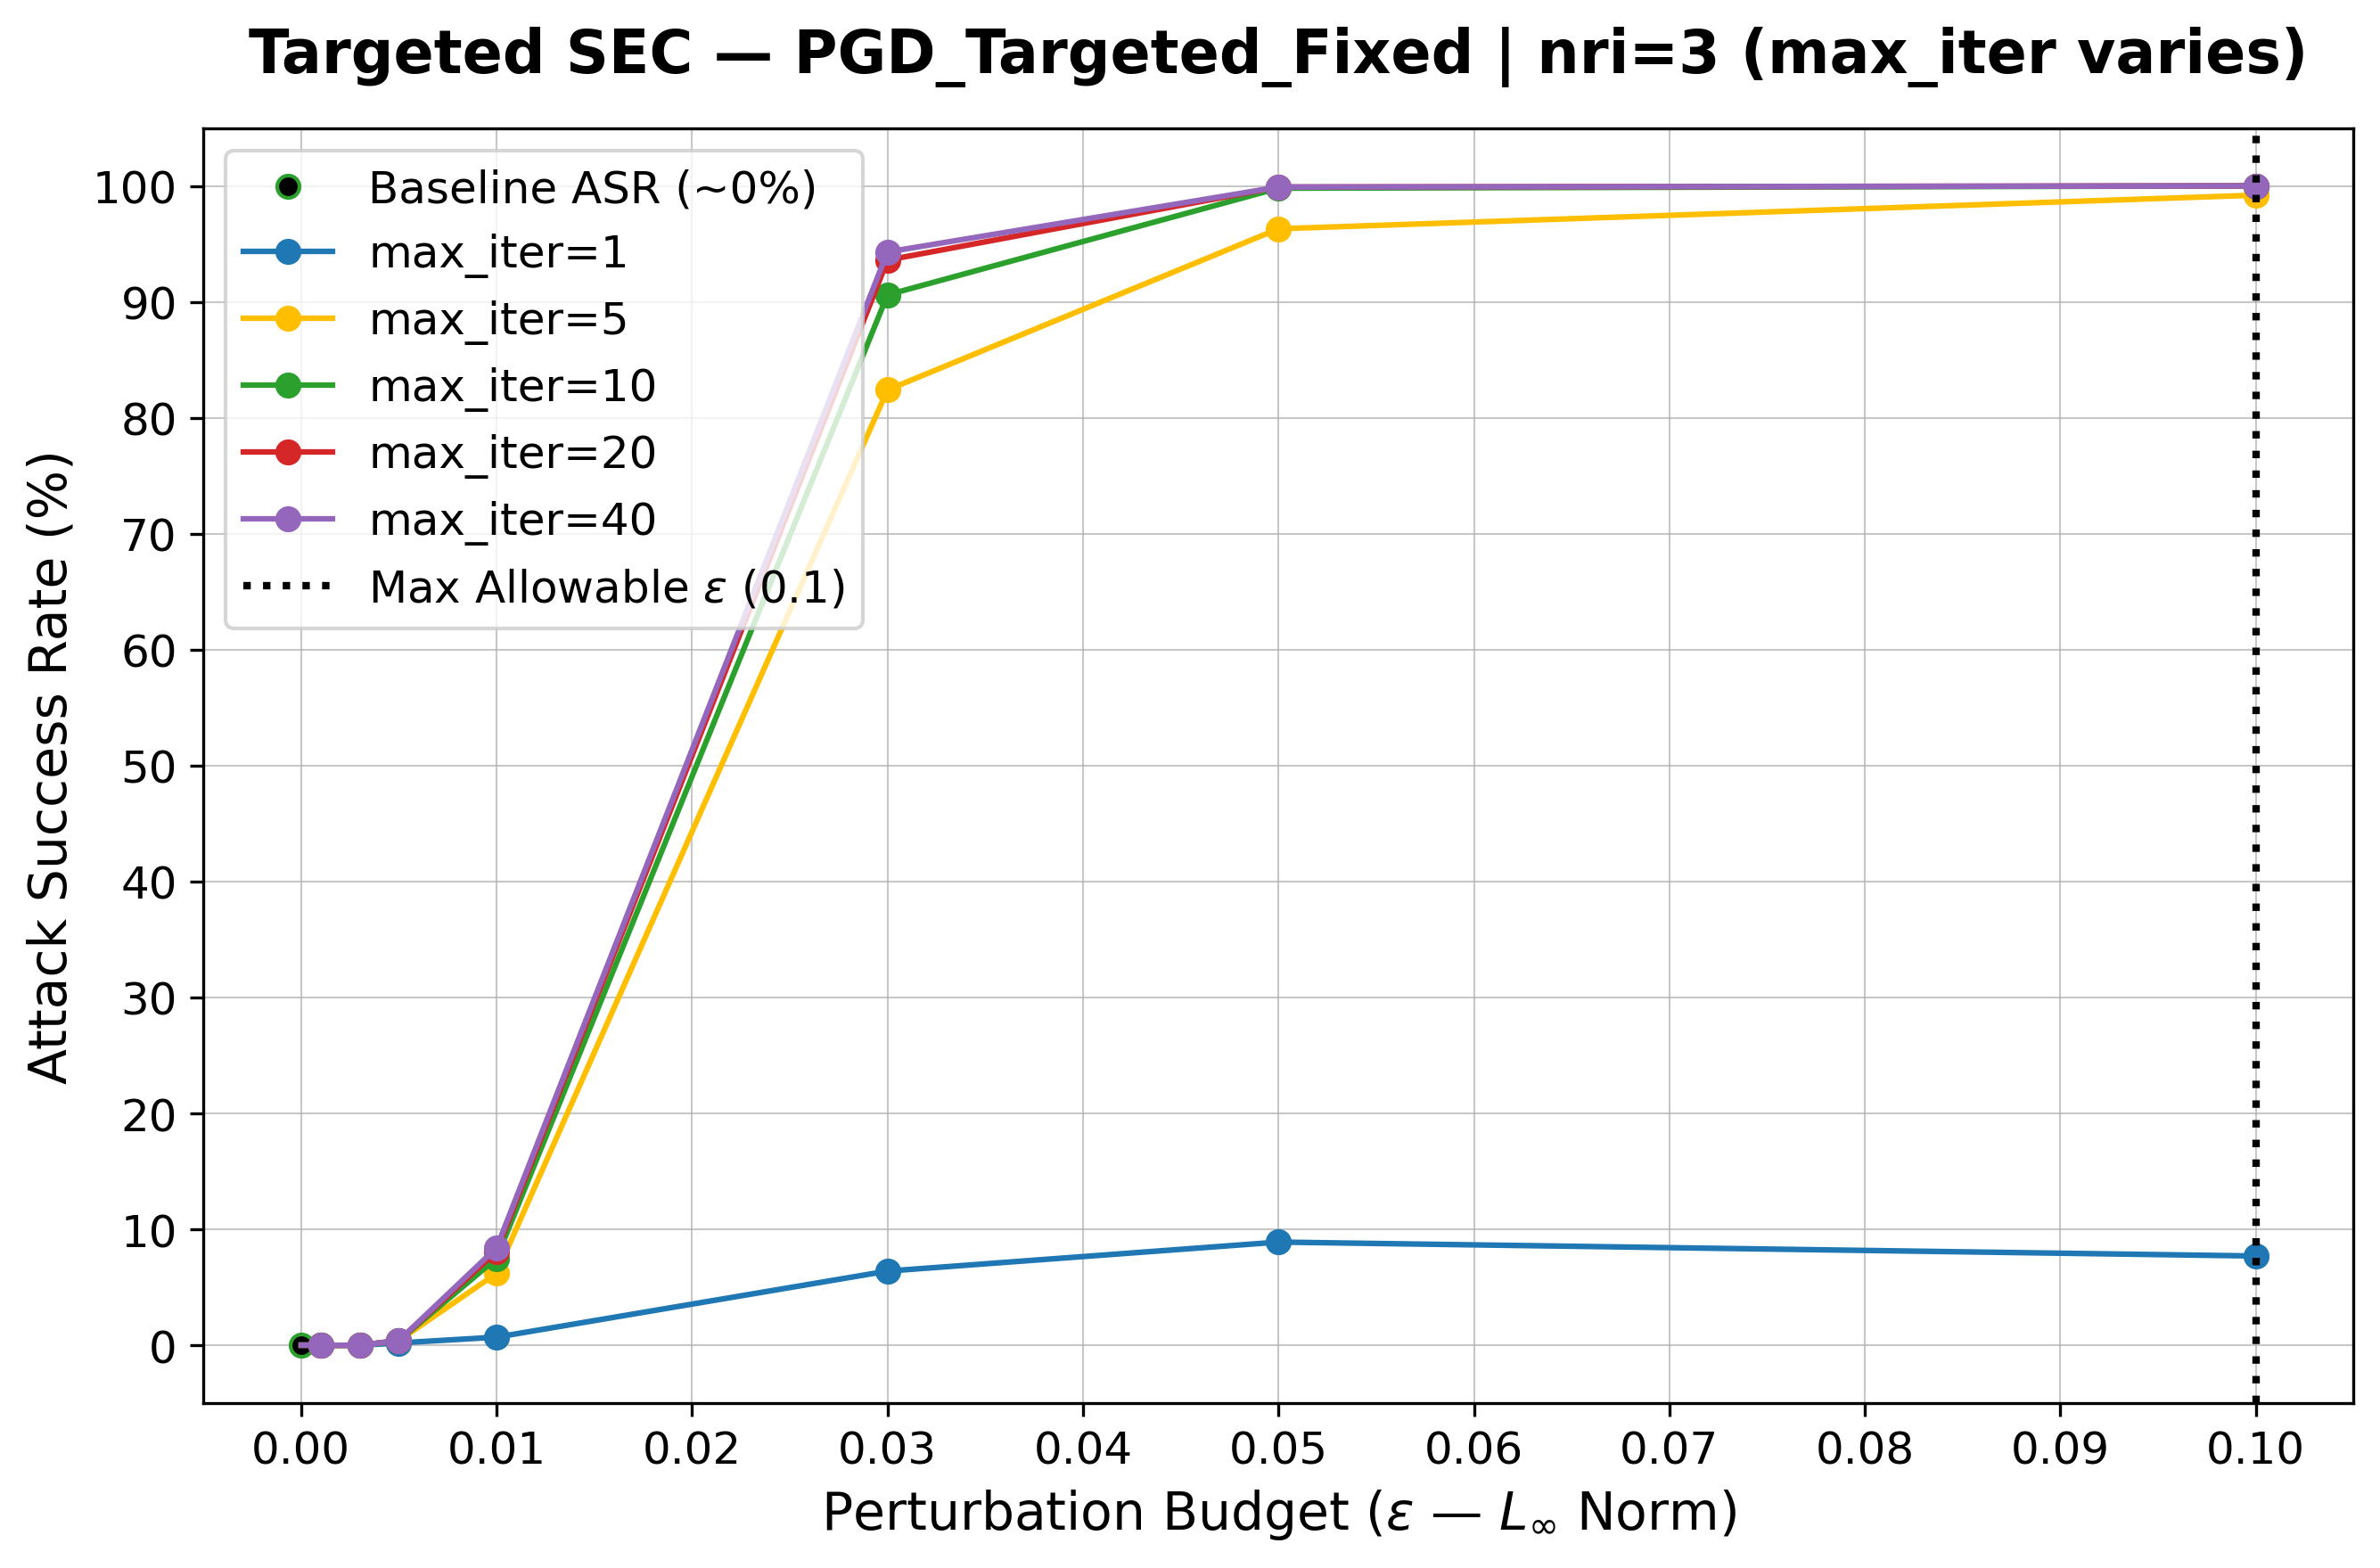
\includegraphics[width=0.5\linewidth]{PGD_Error_specific/Fixed/PGD_Targeted_Fixed_nri3_comparative_maxiter_SEC.png}
    \caption{PGD SEC con nri = 3}
    \label{fig:PGD_SEC_nri3}
\end{figure}

% -- SOTTO GRAFICI PER NRI = 3
\begin{figure}[H]
    \centering
    % Sotto-figura 1
    \begin{subfigure}[b]{0.45\textwidth}
        \centering
        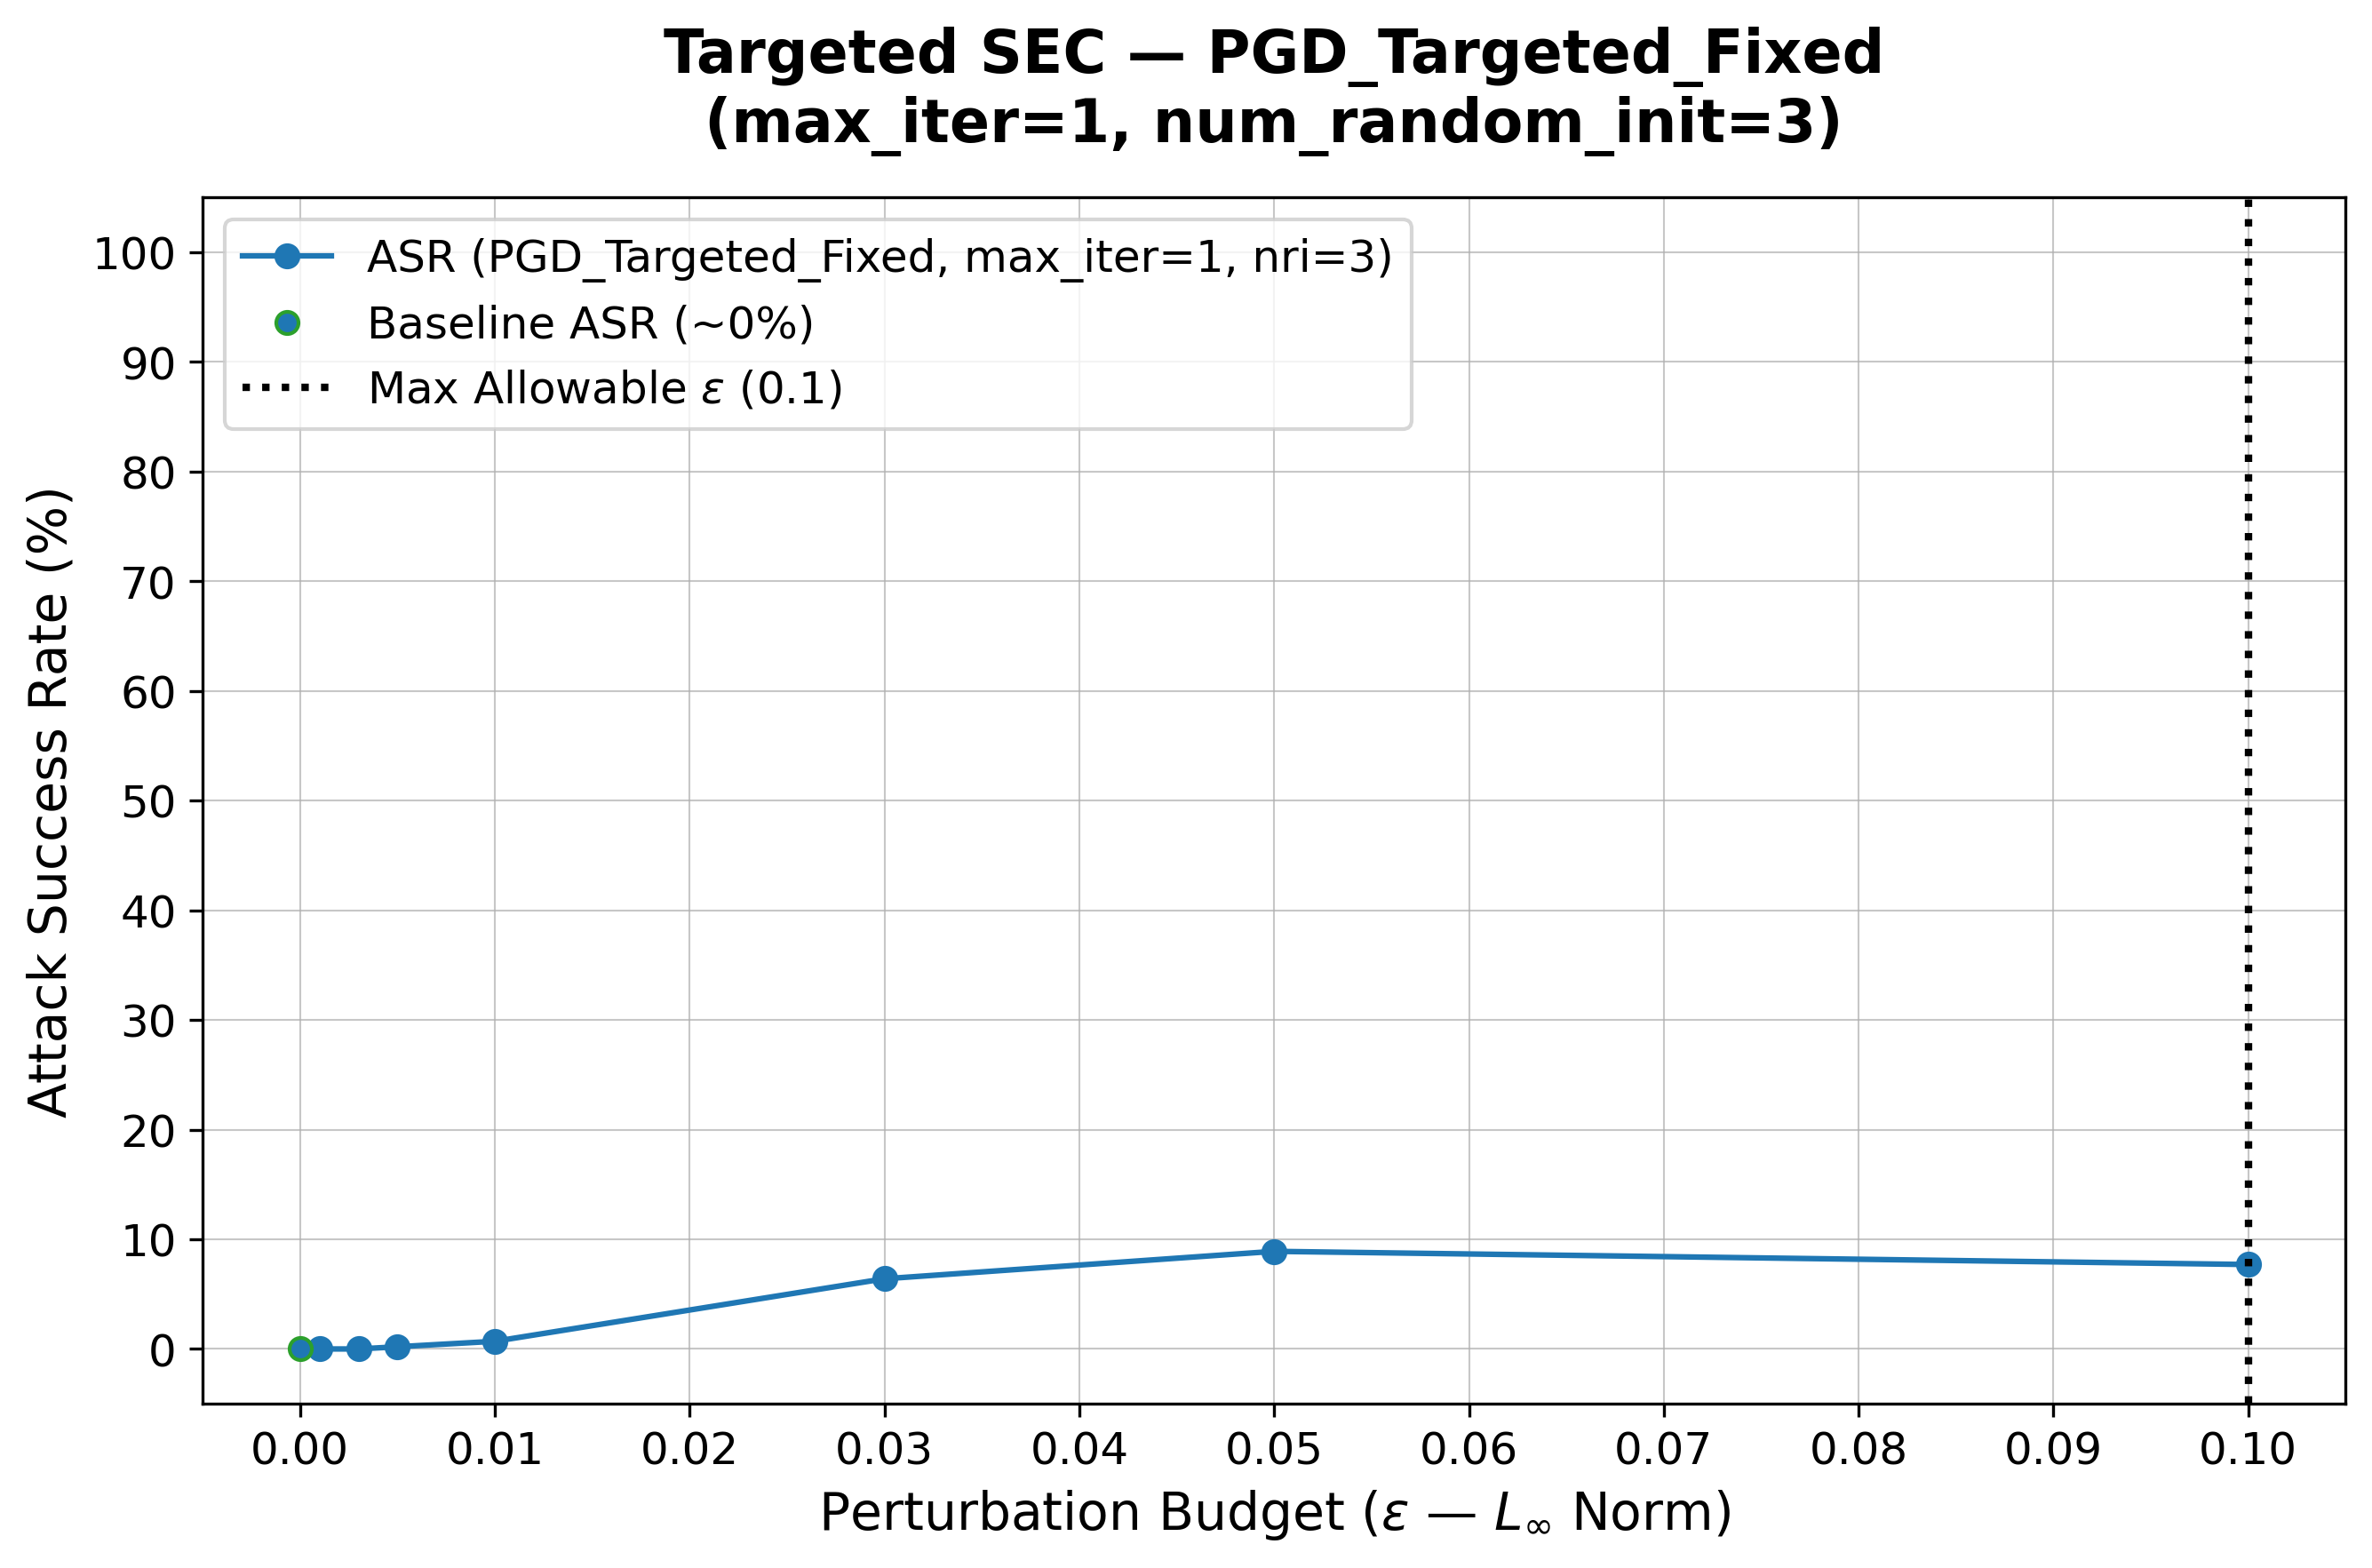
\includegraphics[width=\textwidth]{PGD_Error_specific/Fixed/PGD_Targeted_Fixed_nri3_iter1_SEC.png}
        \caption{\texttt{max_iter} = 1}
        \label{fig:PGD_nri3_iter1}
    \end{subfigure}
    \hfill
    % Sotto-figura 2
    \begin{subfigure}[b]{0.45\textwidth}
        \centering
        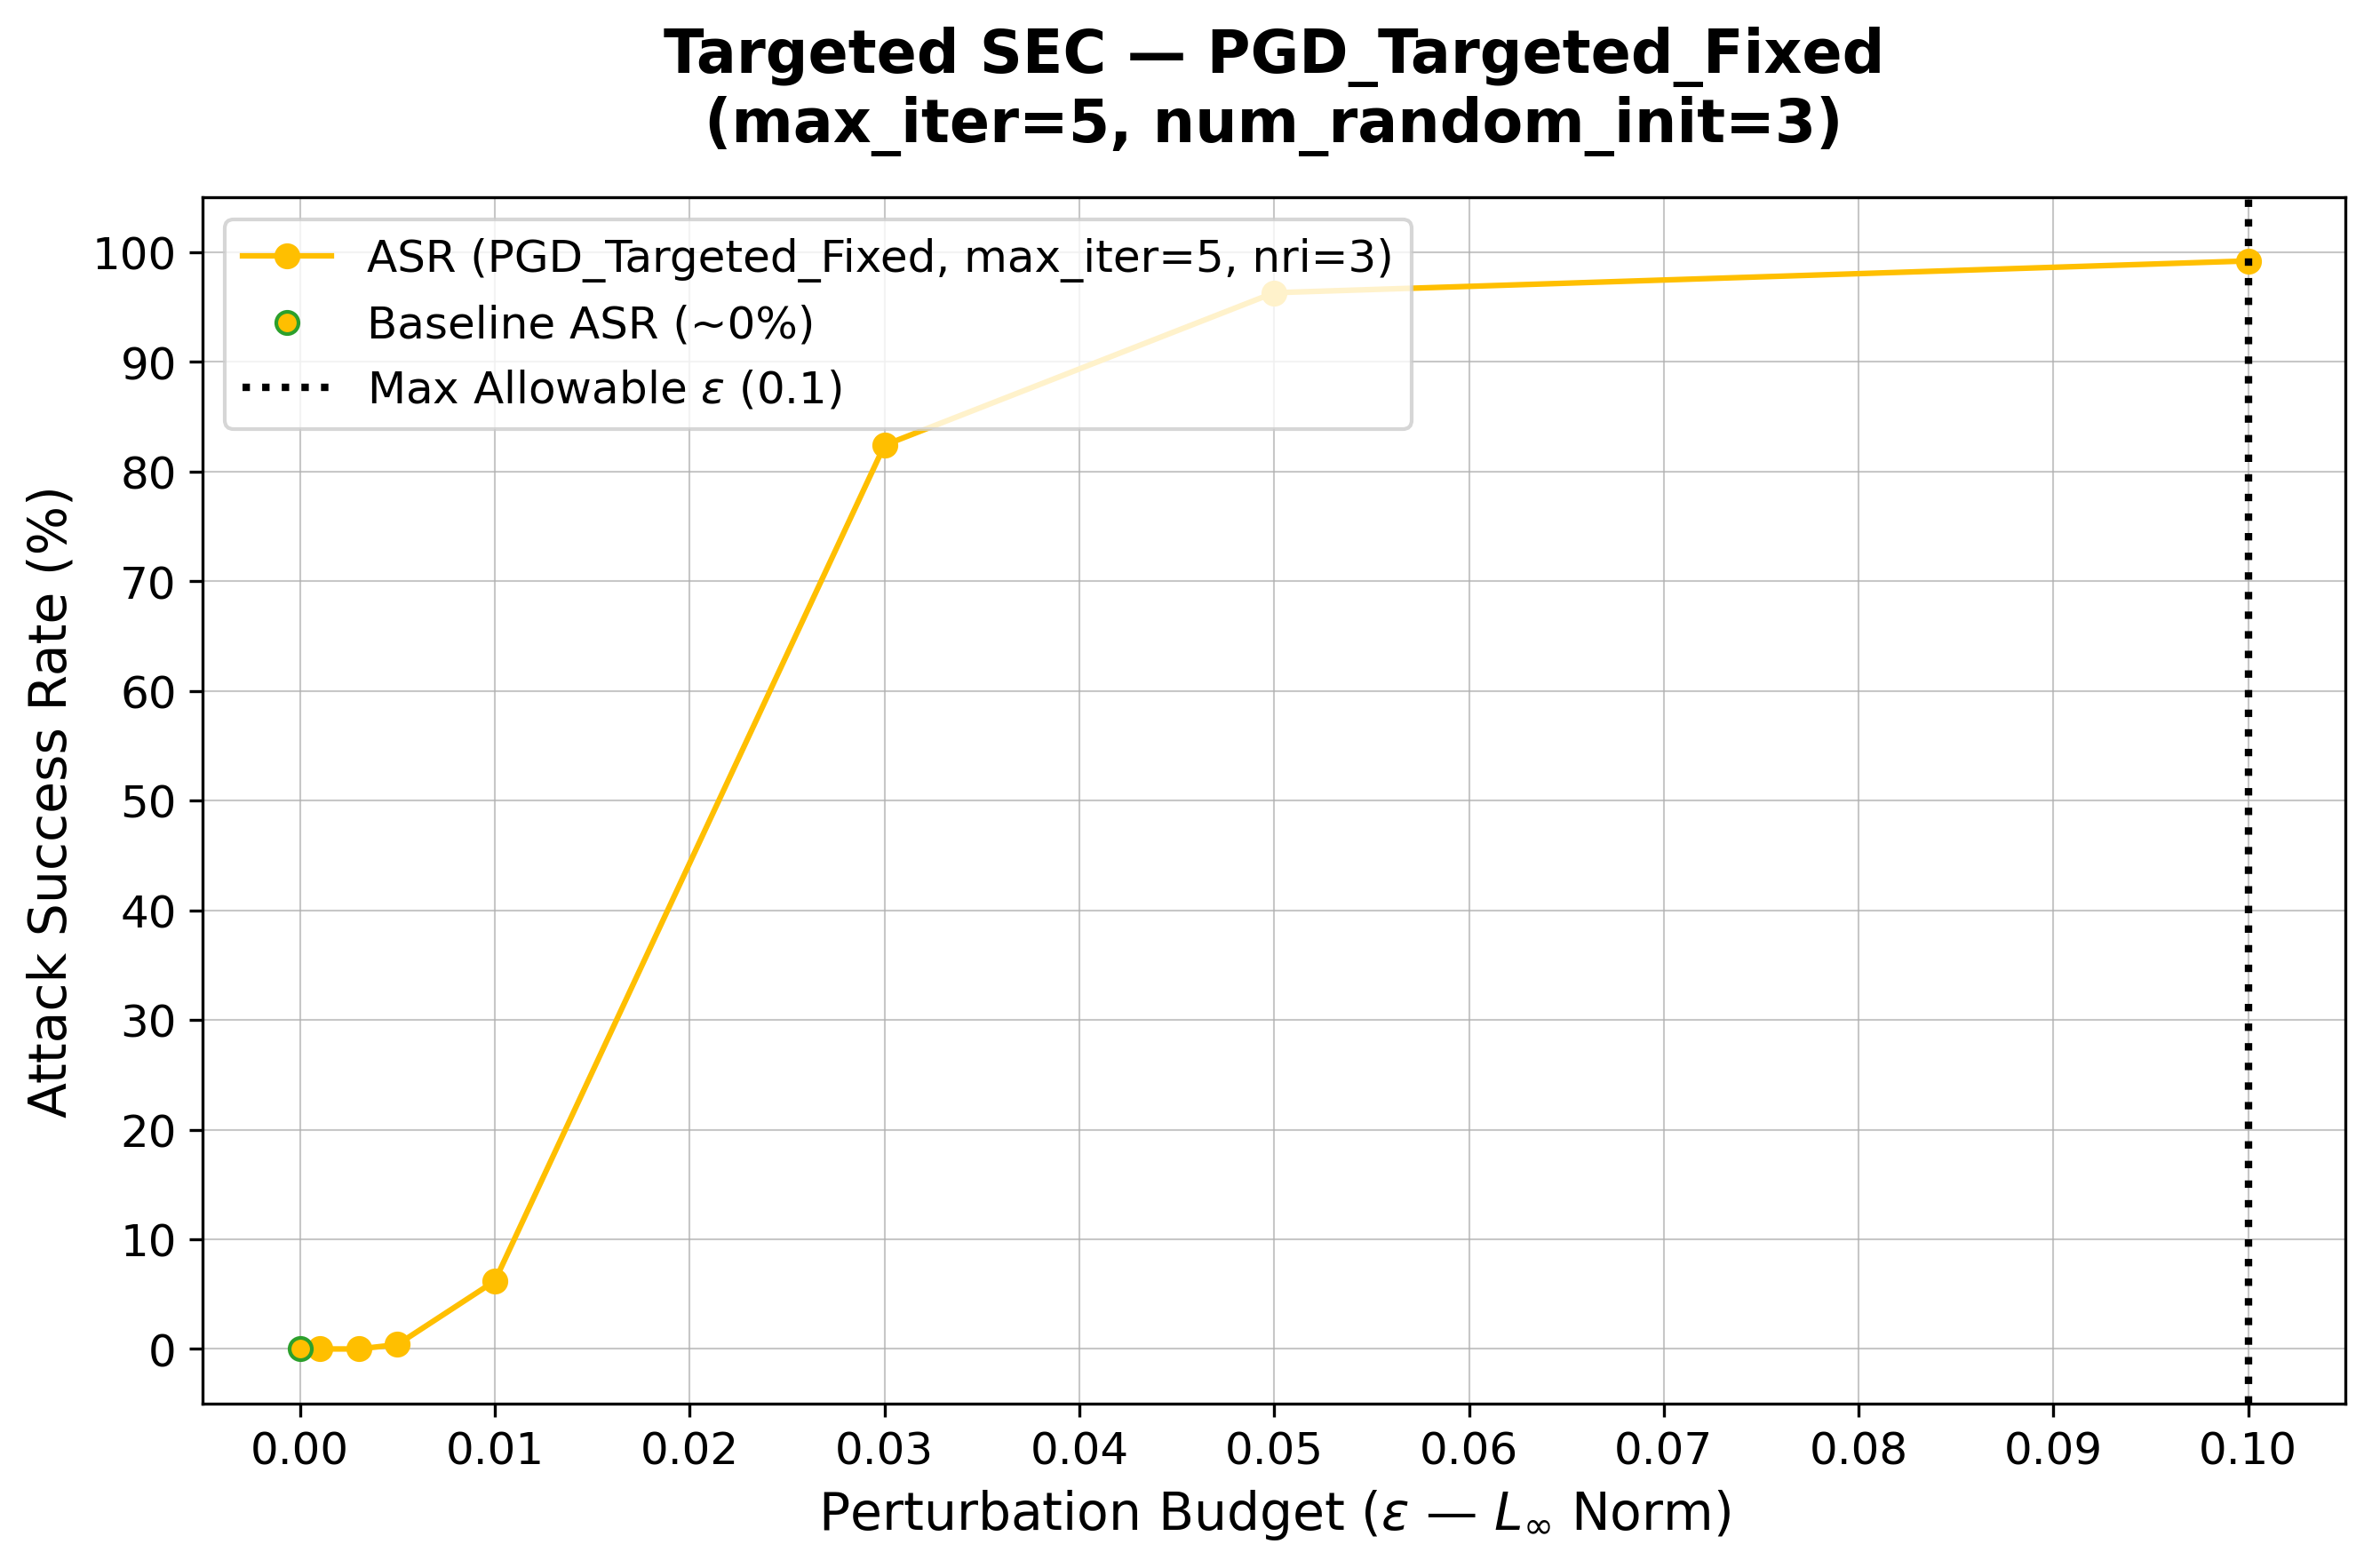
\includegraphics[width=\textwidth]{PGD_Error_specific/Fixed/PGD_Targeted_Fixed_nri3_iter5_SEC.png}
        \caption{\texttt{max_iter} = 5}
        \label{fig:PGD_nri3_iter5}
    \end{subfigure}

    \vspace{1em} % Spazio verticale tra le righe di immagini
    % Sotto-figura 3
    \begin{subfigure}[b]{0.45\textwidth}
        \centering
        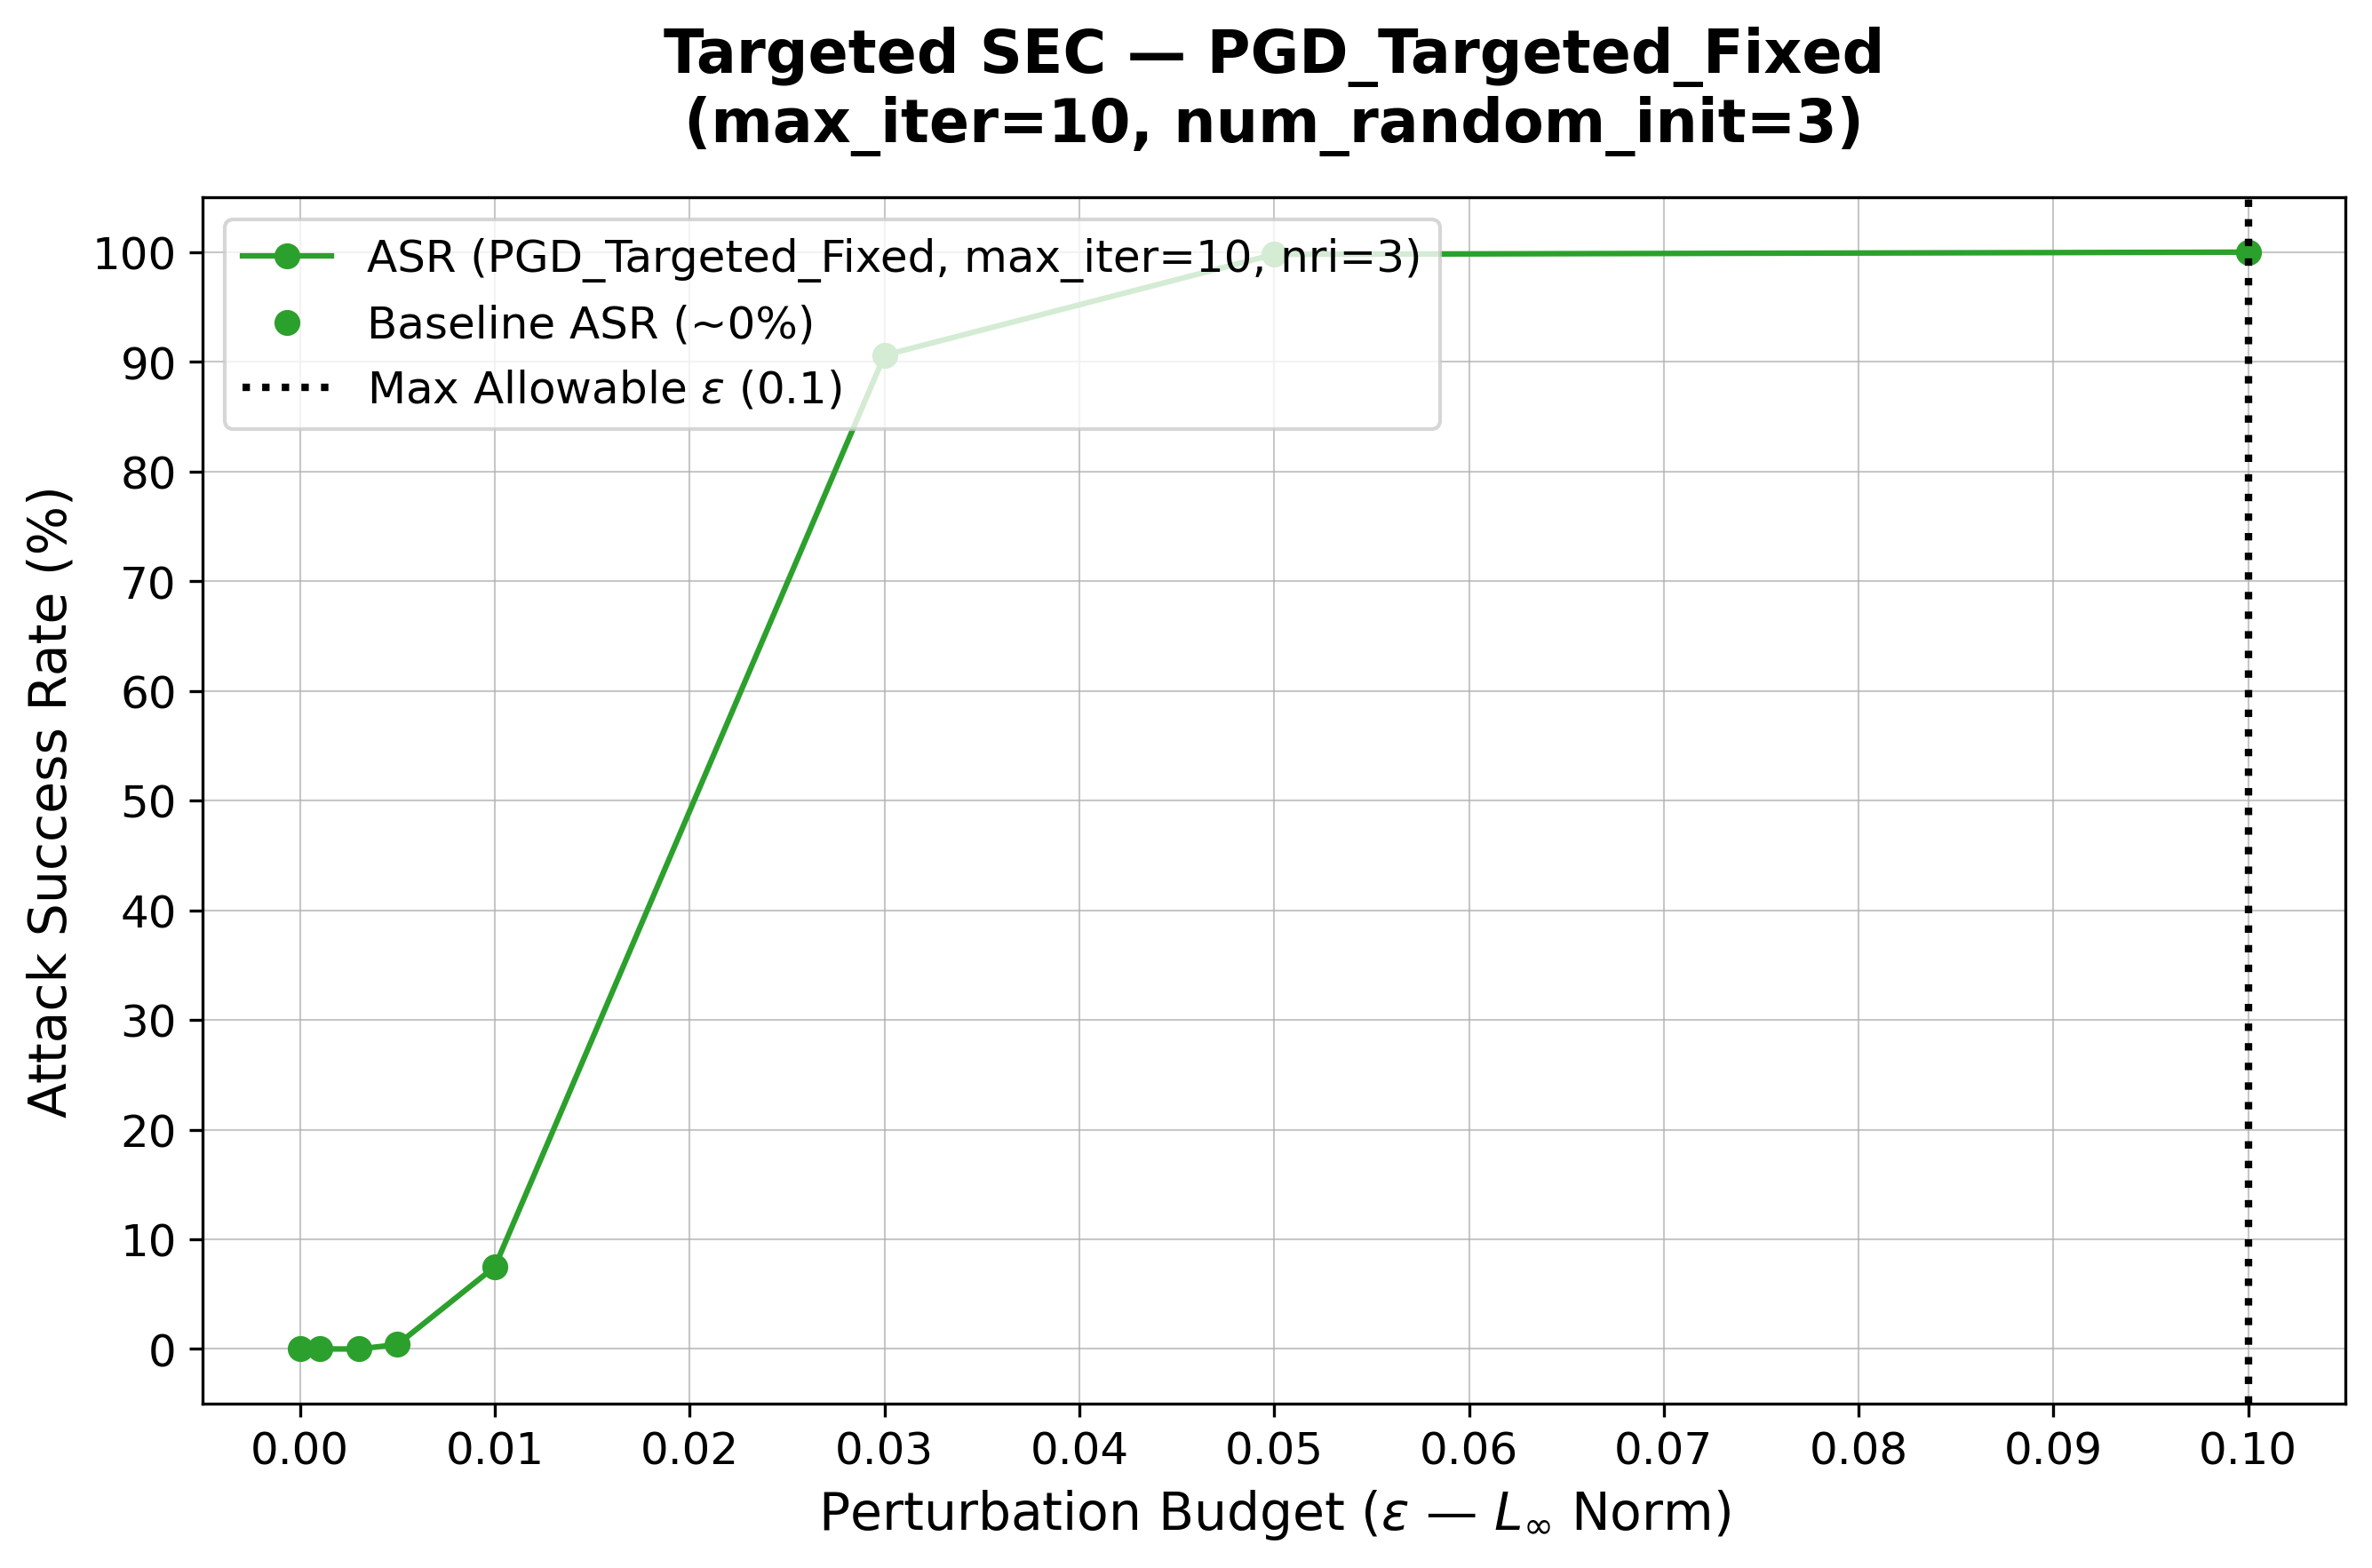
\includegraphics[width=\textwidth]{PGD_Error_specific/Fixed/PGD_Targeted_Fixed_nri3_iter10_SEC.png}
        \caption{\texttt{max_iter} = 10}
        \label{fig:PGD_nri3_iter10}
    \end{subfigure}
    \hfill
    % Sotto-figura 4
    \begin{subfigure}[b]{0.45\textwidth}
        \centering
        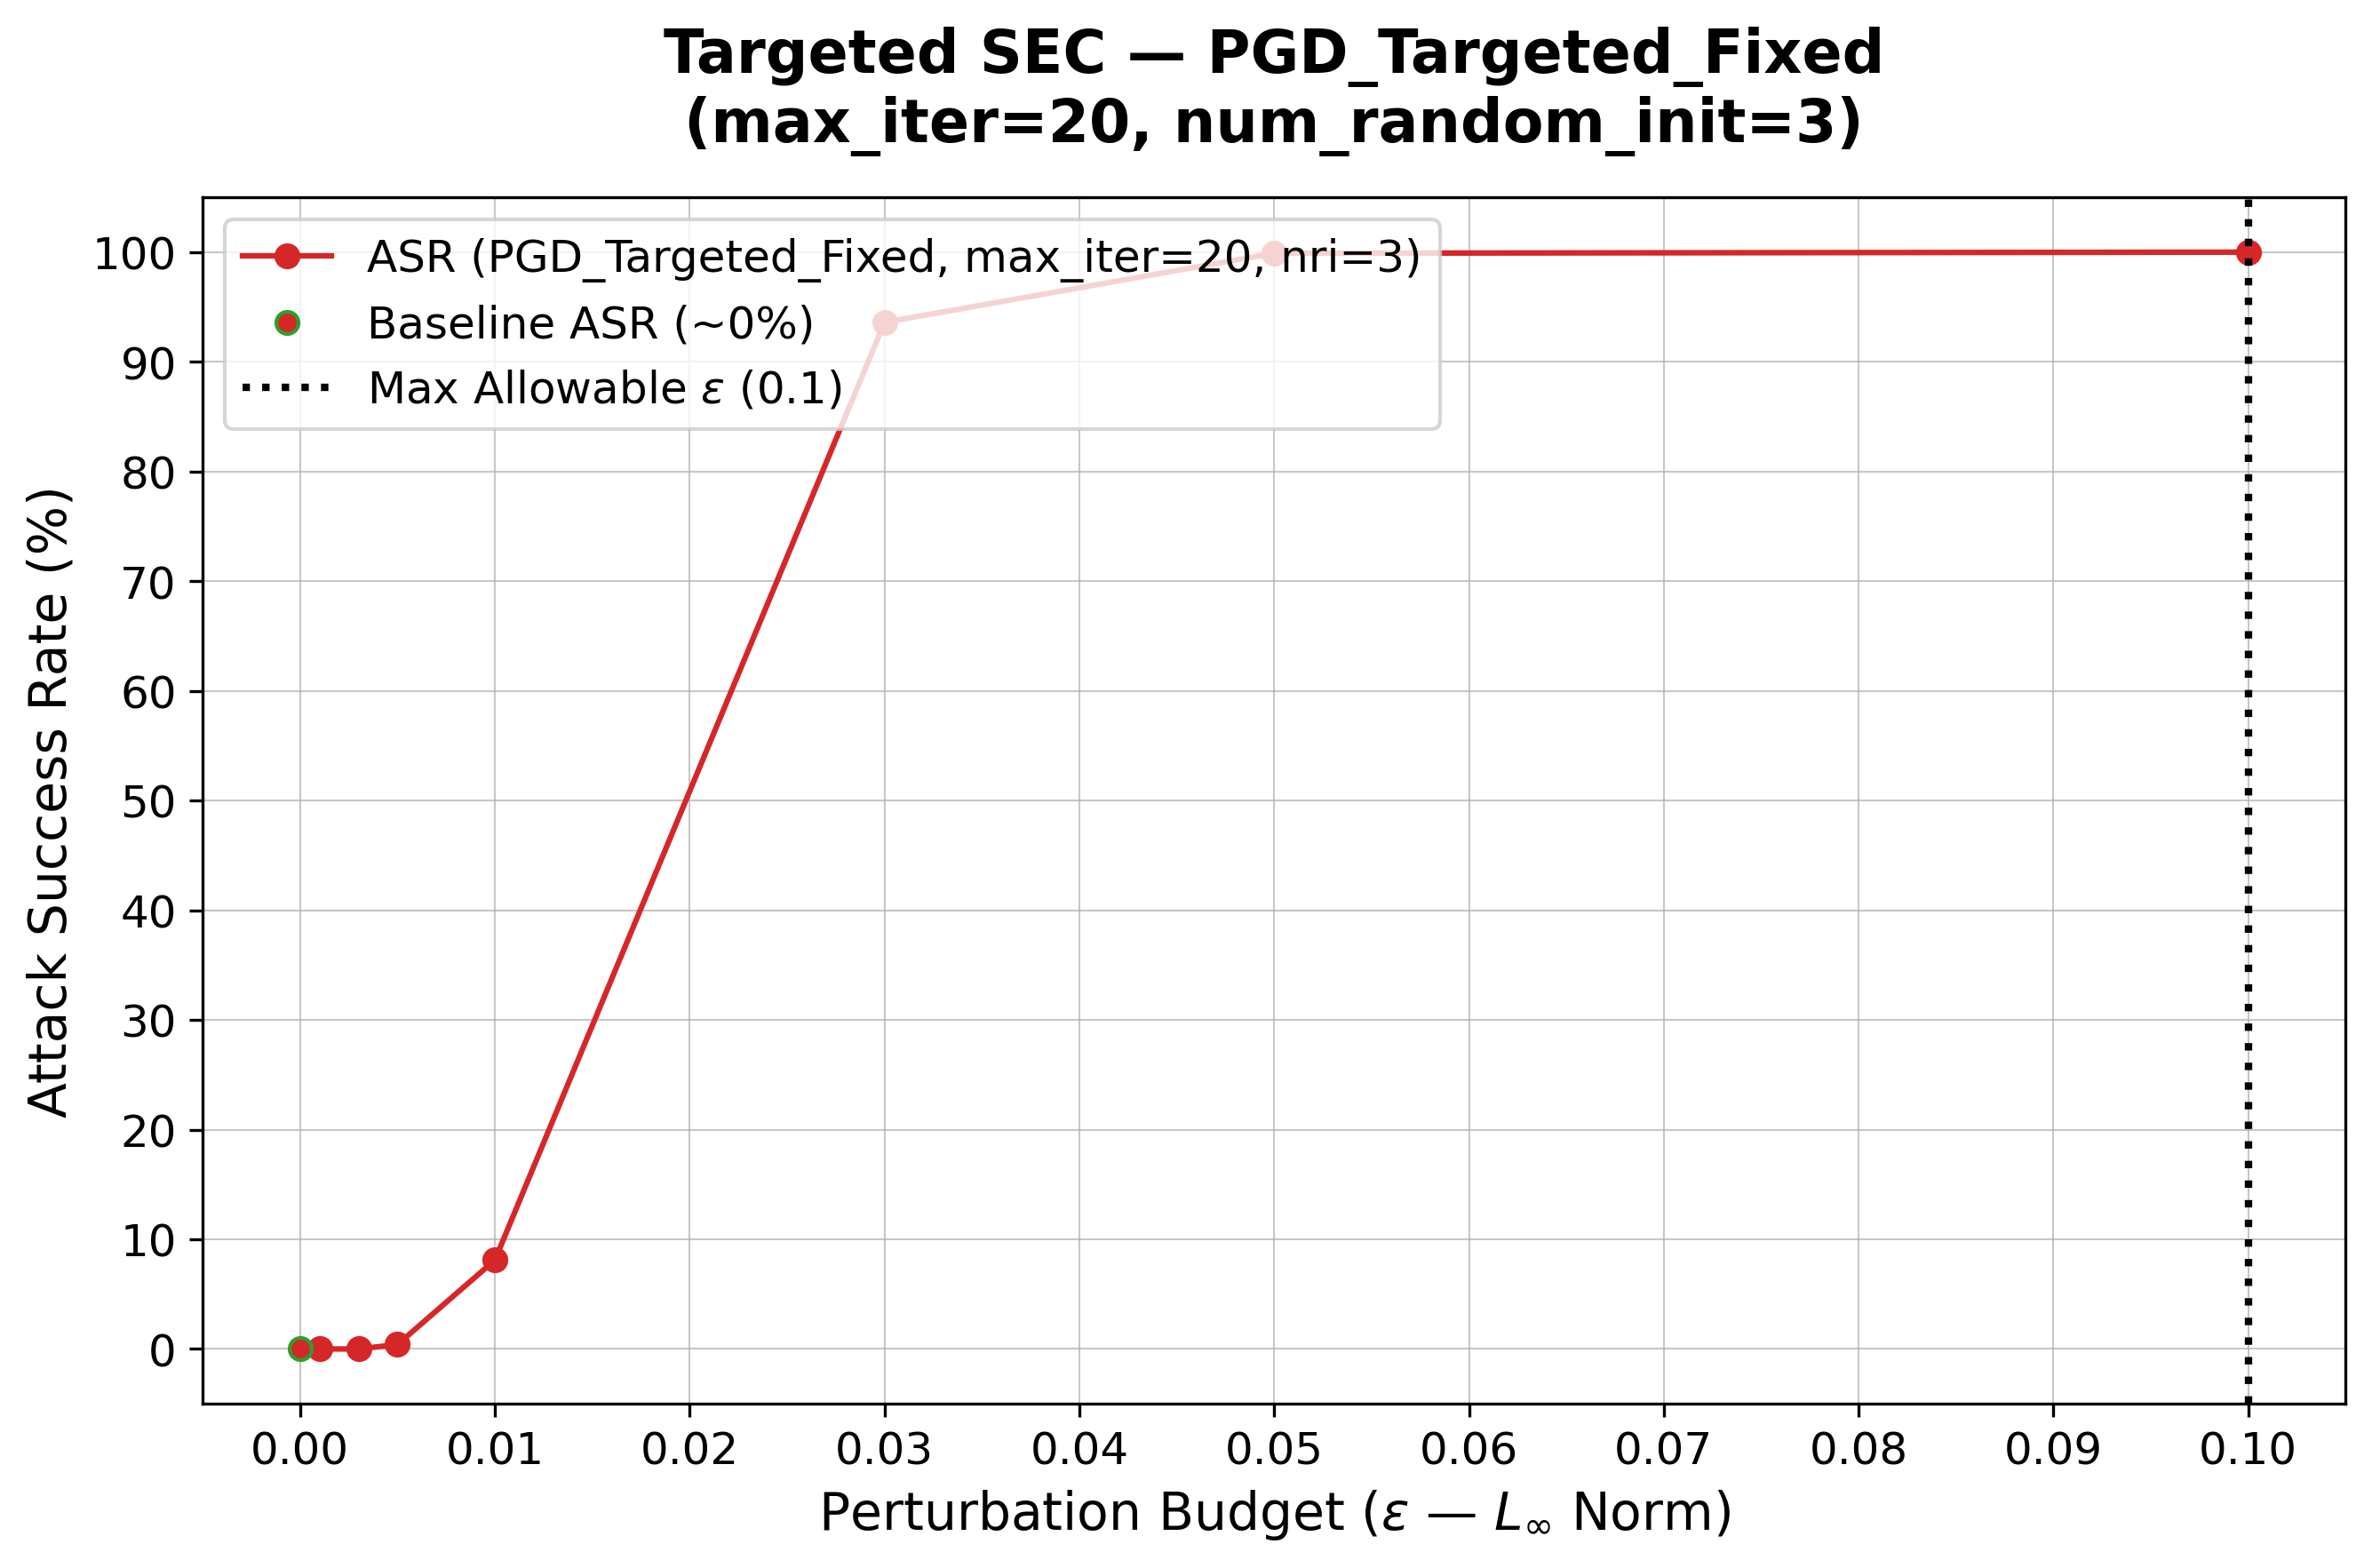
\includegraphics[width=\textwidth]{PGD_Error_specific/Fixed/PGD_Targeted_Fixed_nri3_iter20_SEC.png}
        \caption{\texttt{max_iter} = 20}
        \label{fig:PGD_nri3_iter20}
    \end{subfigure}
    \vspace{1em} % Spazio verticale tra le righe di immagini
    % Sotto-figura 5
    \begin{subfigure}[b]{0.45\textwidth}
        \centering
        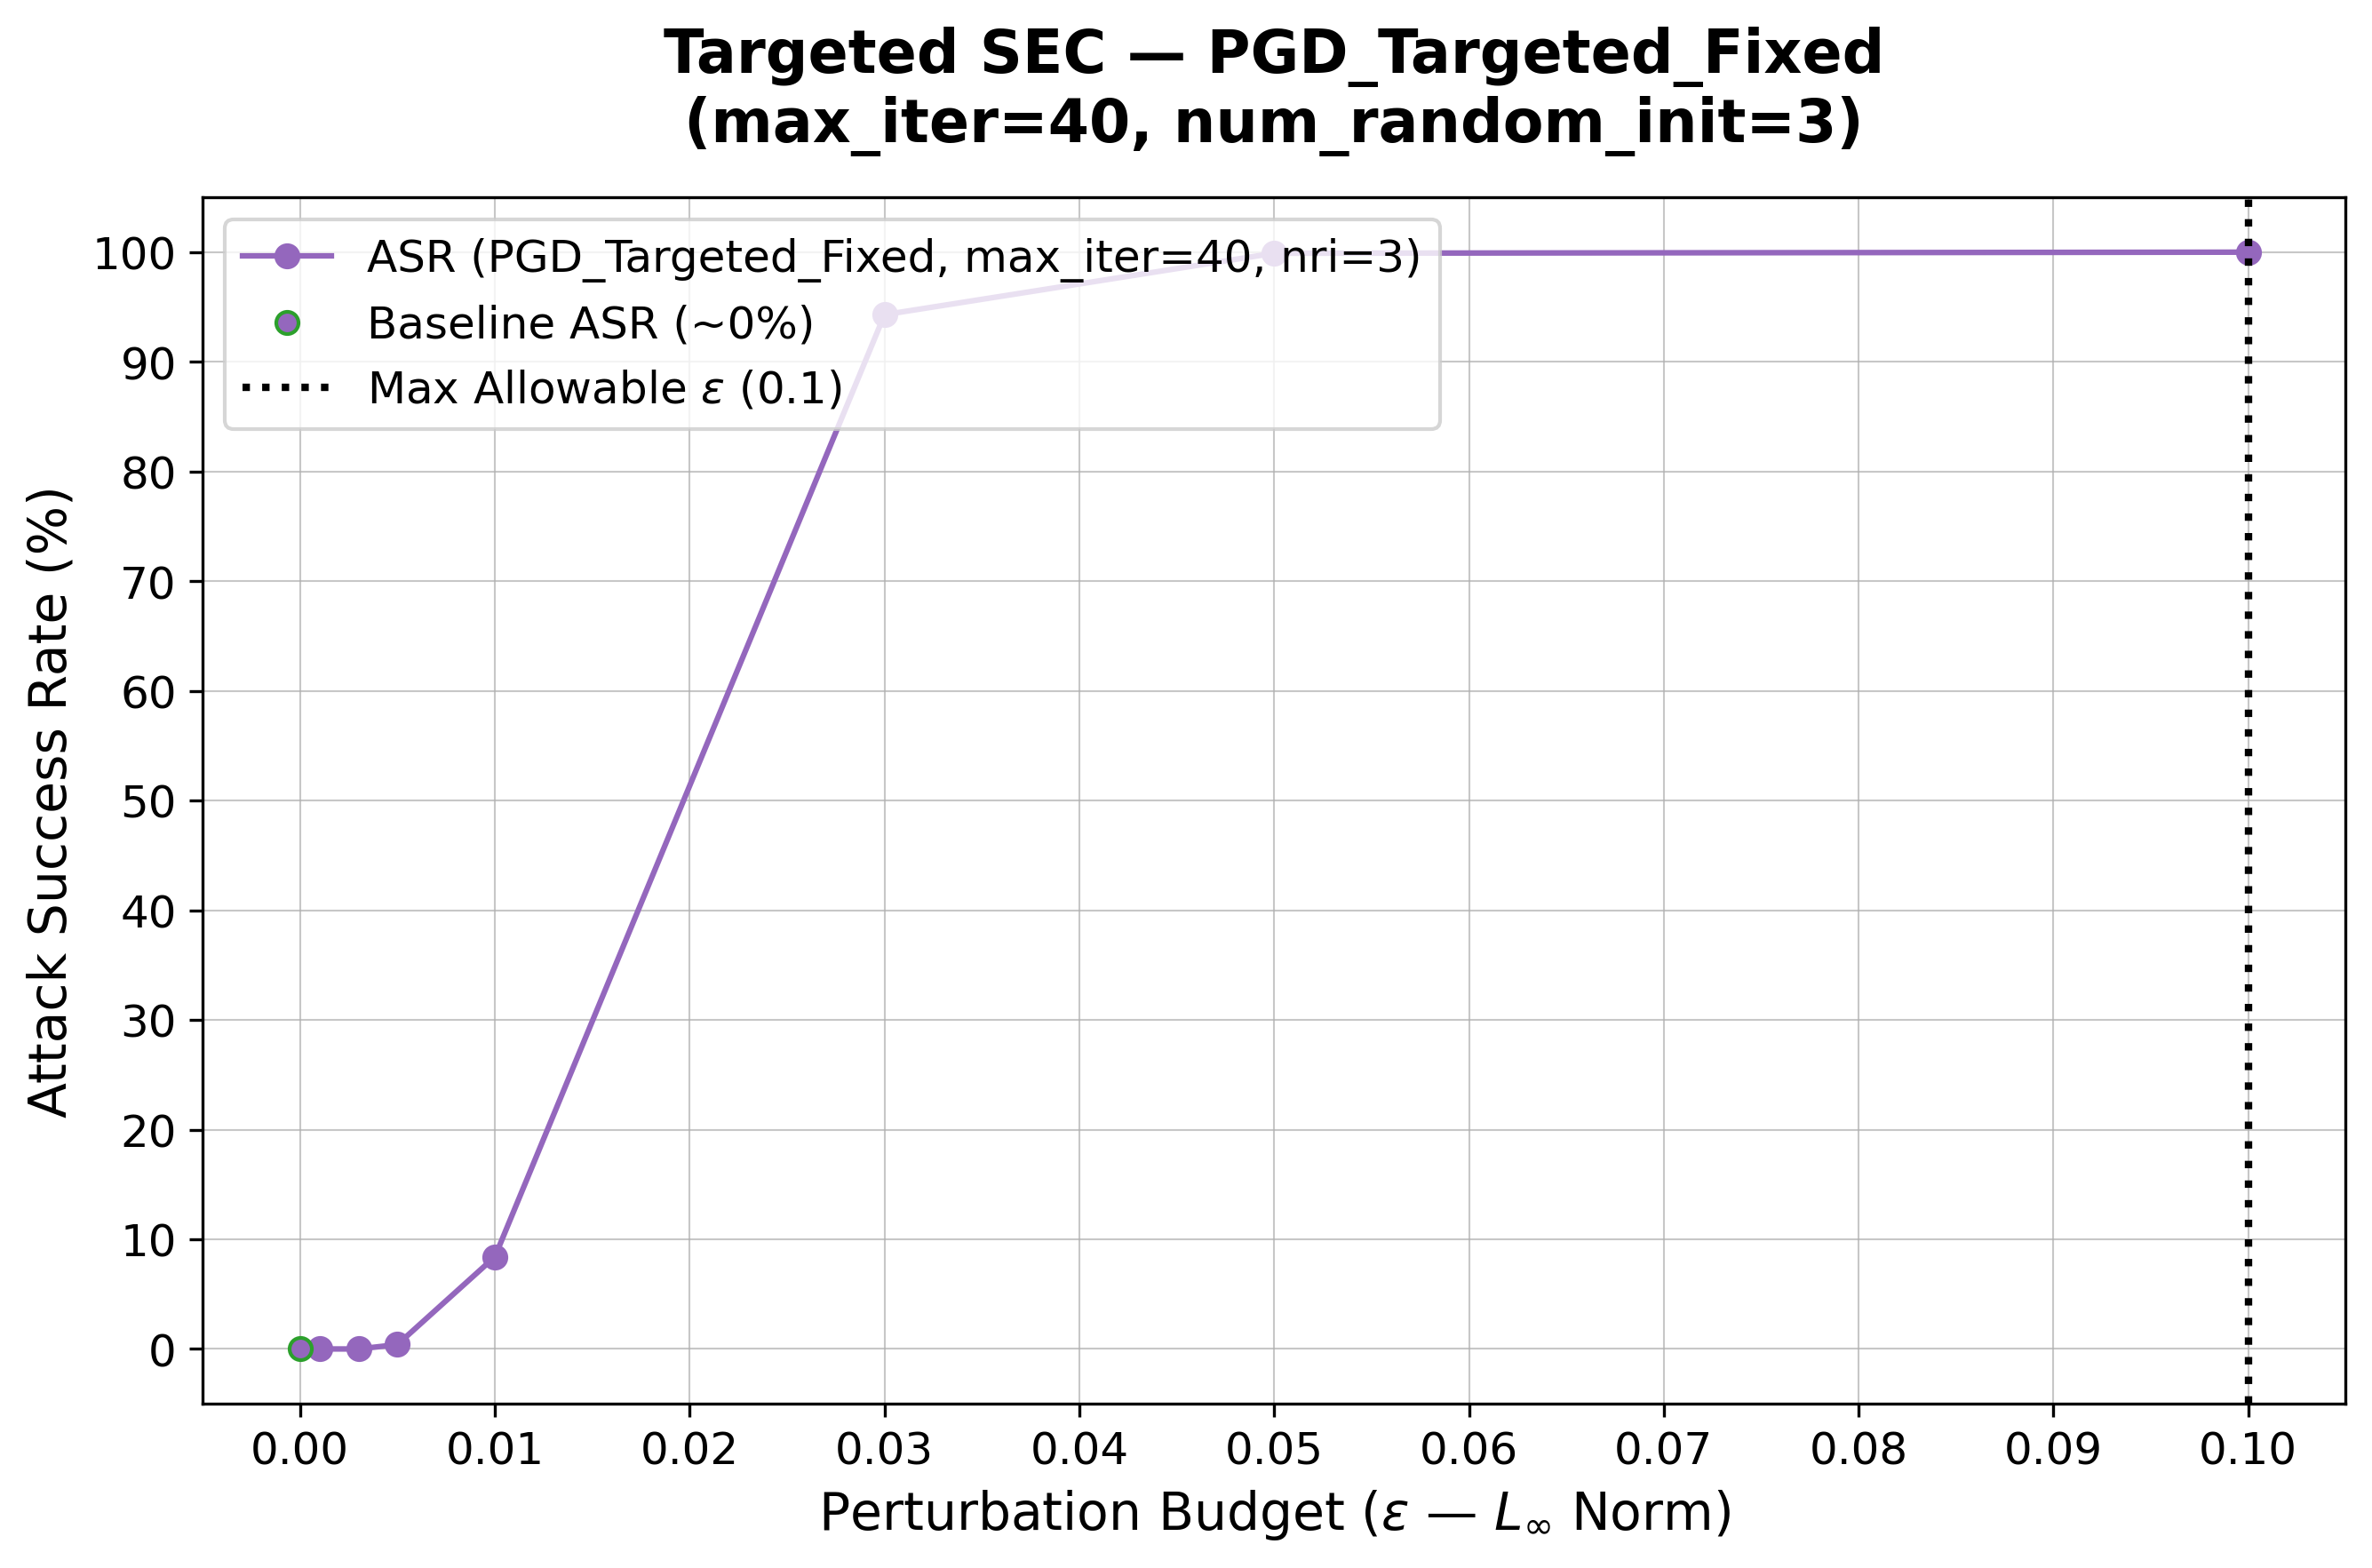
\includegraphics[width=\textwidth]{PGD_Error_specific/Fixed/PGD_Targeted_Fixed_nri3_iter40_SEC.png}
        \caption{\texttt{max_iter} = 40}
        \label{fig:PGD_nri3_iter40}
    \end{subfigure}
    \caption{PGD Fixed - Iterazioni a confronto per \texttt{nri} = 3}
    \label{fig:PGD_iterations_nri3}
\end{figure}

% -- SEC NRI = 5 --
\begin{figure}[H]
    \centering
    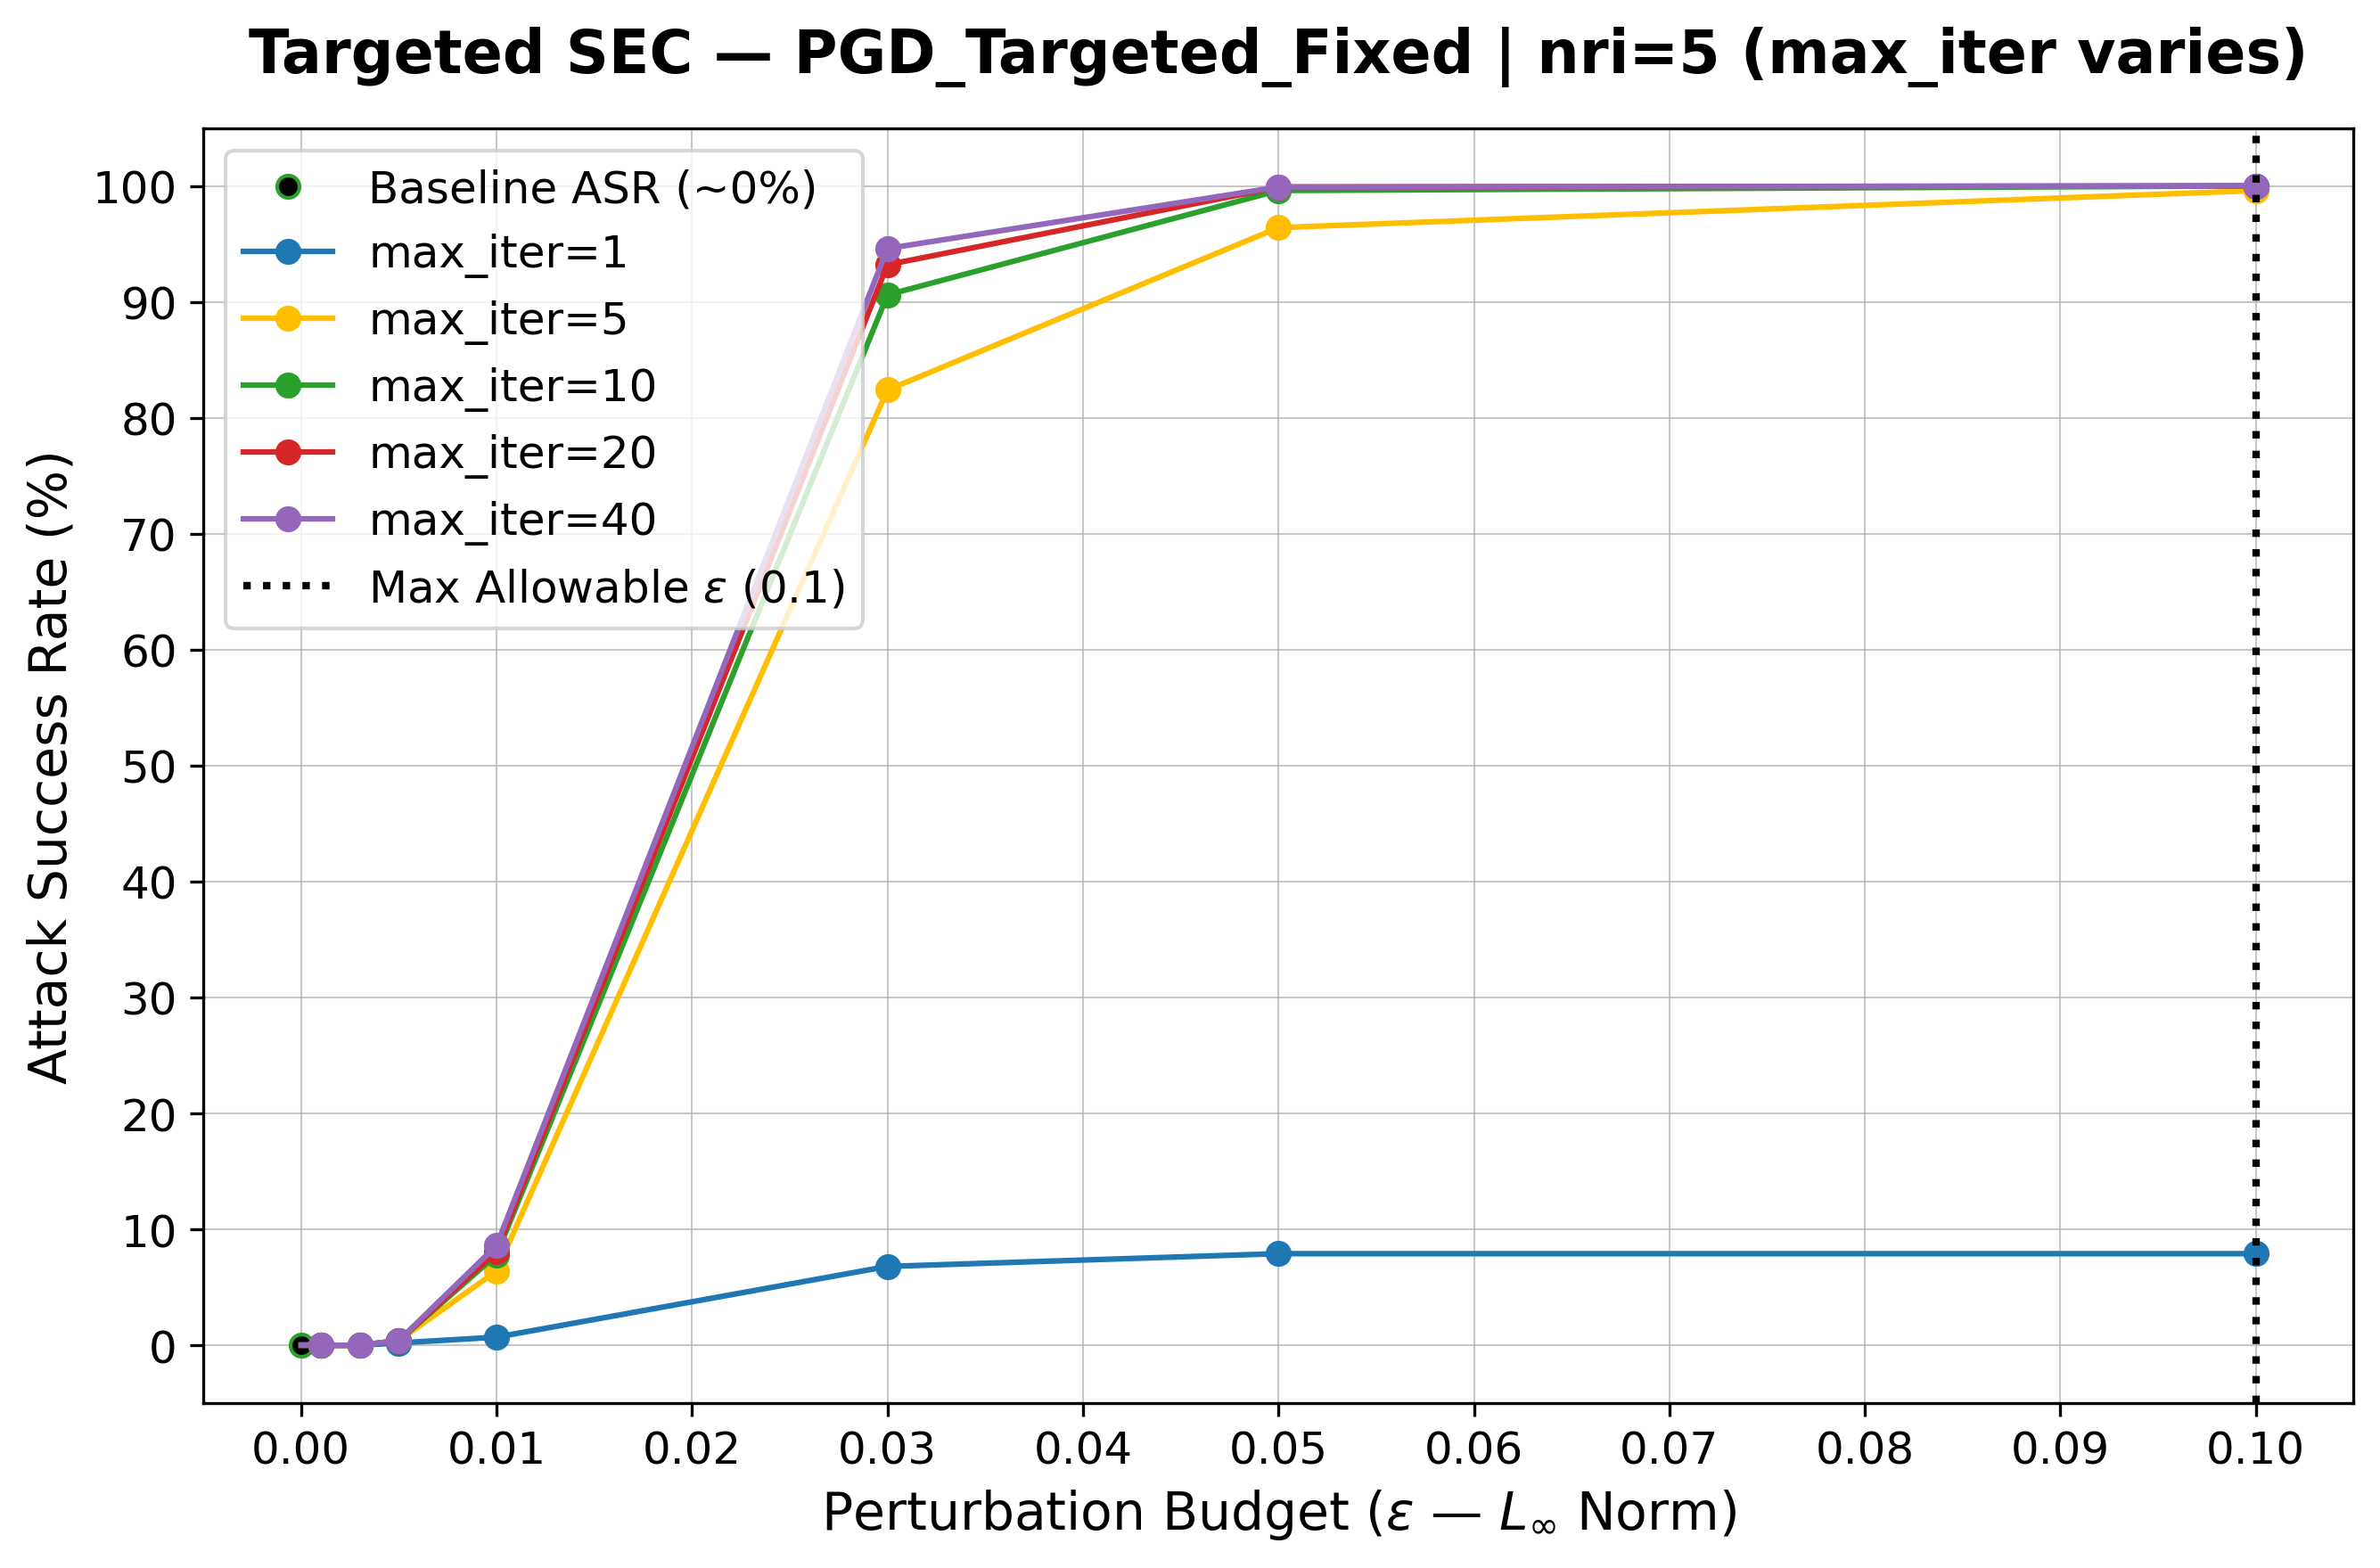
\includegraphics[width=0.5\linewidth]{PGD_Error_specific/Fixed/PGD_Targeted_Fixed_nri5_comparative_maxiter_SEC.png}
    \caption{PGD SEC con nri = 5}
    \label{fig:PGD_SEC_nri5}
\end{figure}

% -- SOTTO GRAFICI PER NRI = 5
\begin{figure}[H]
    \centering
    % Sotto-figura 1
    \begin{subfigure}[b]{0.45\textwidth}
        \centering
        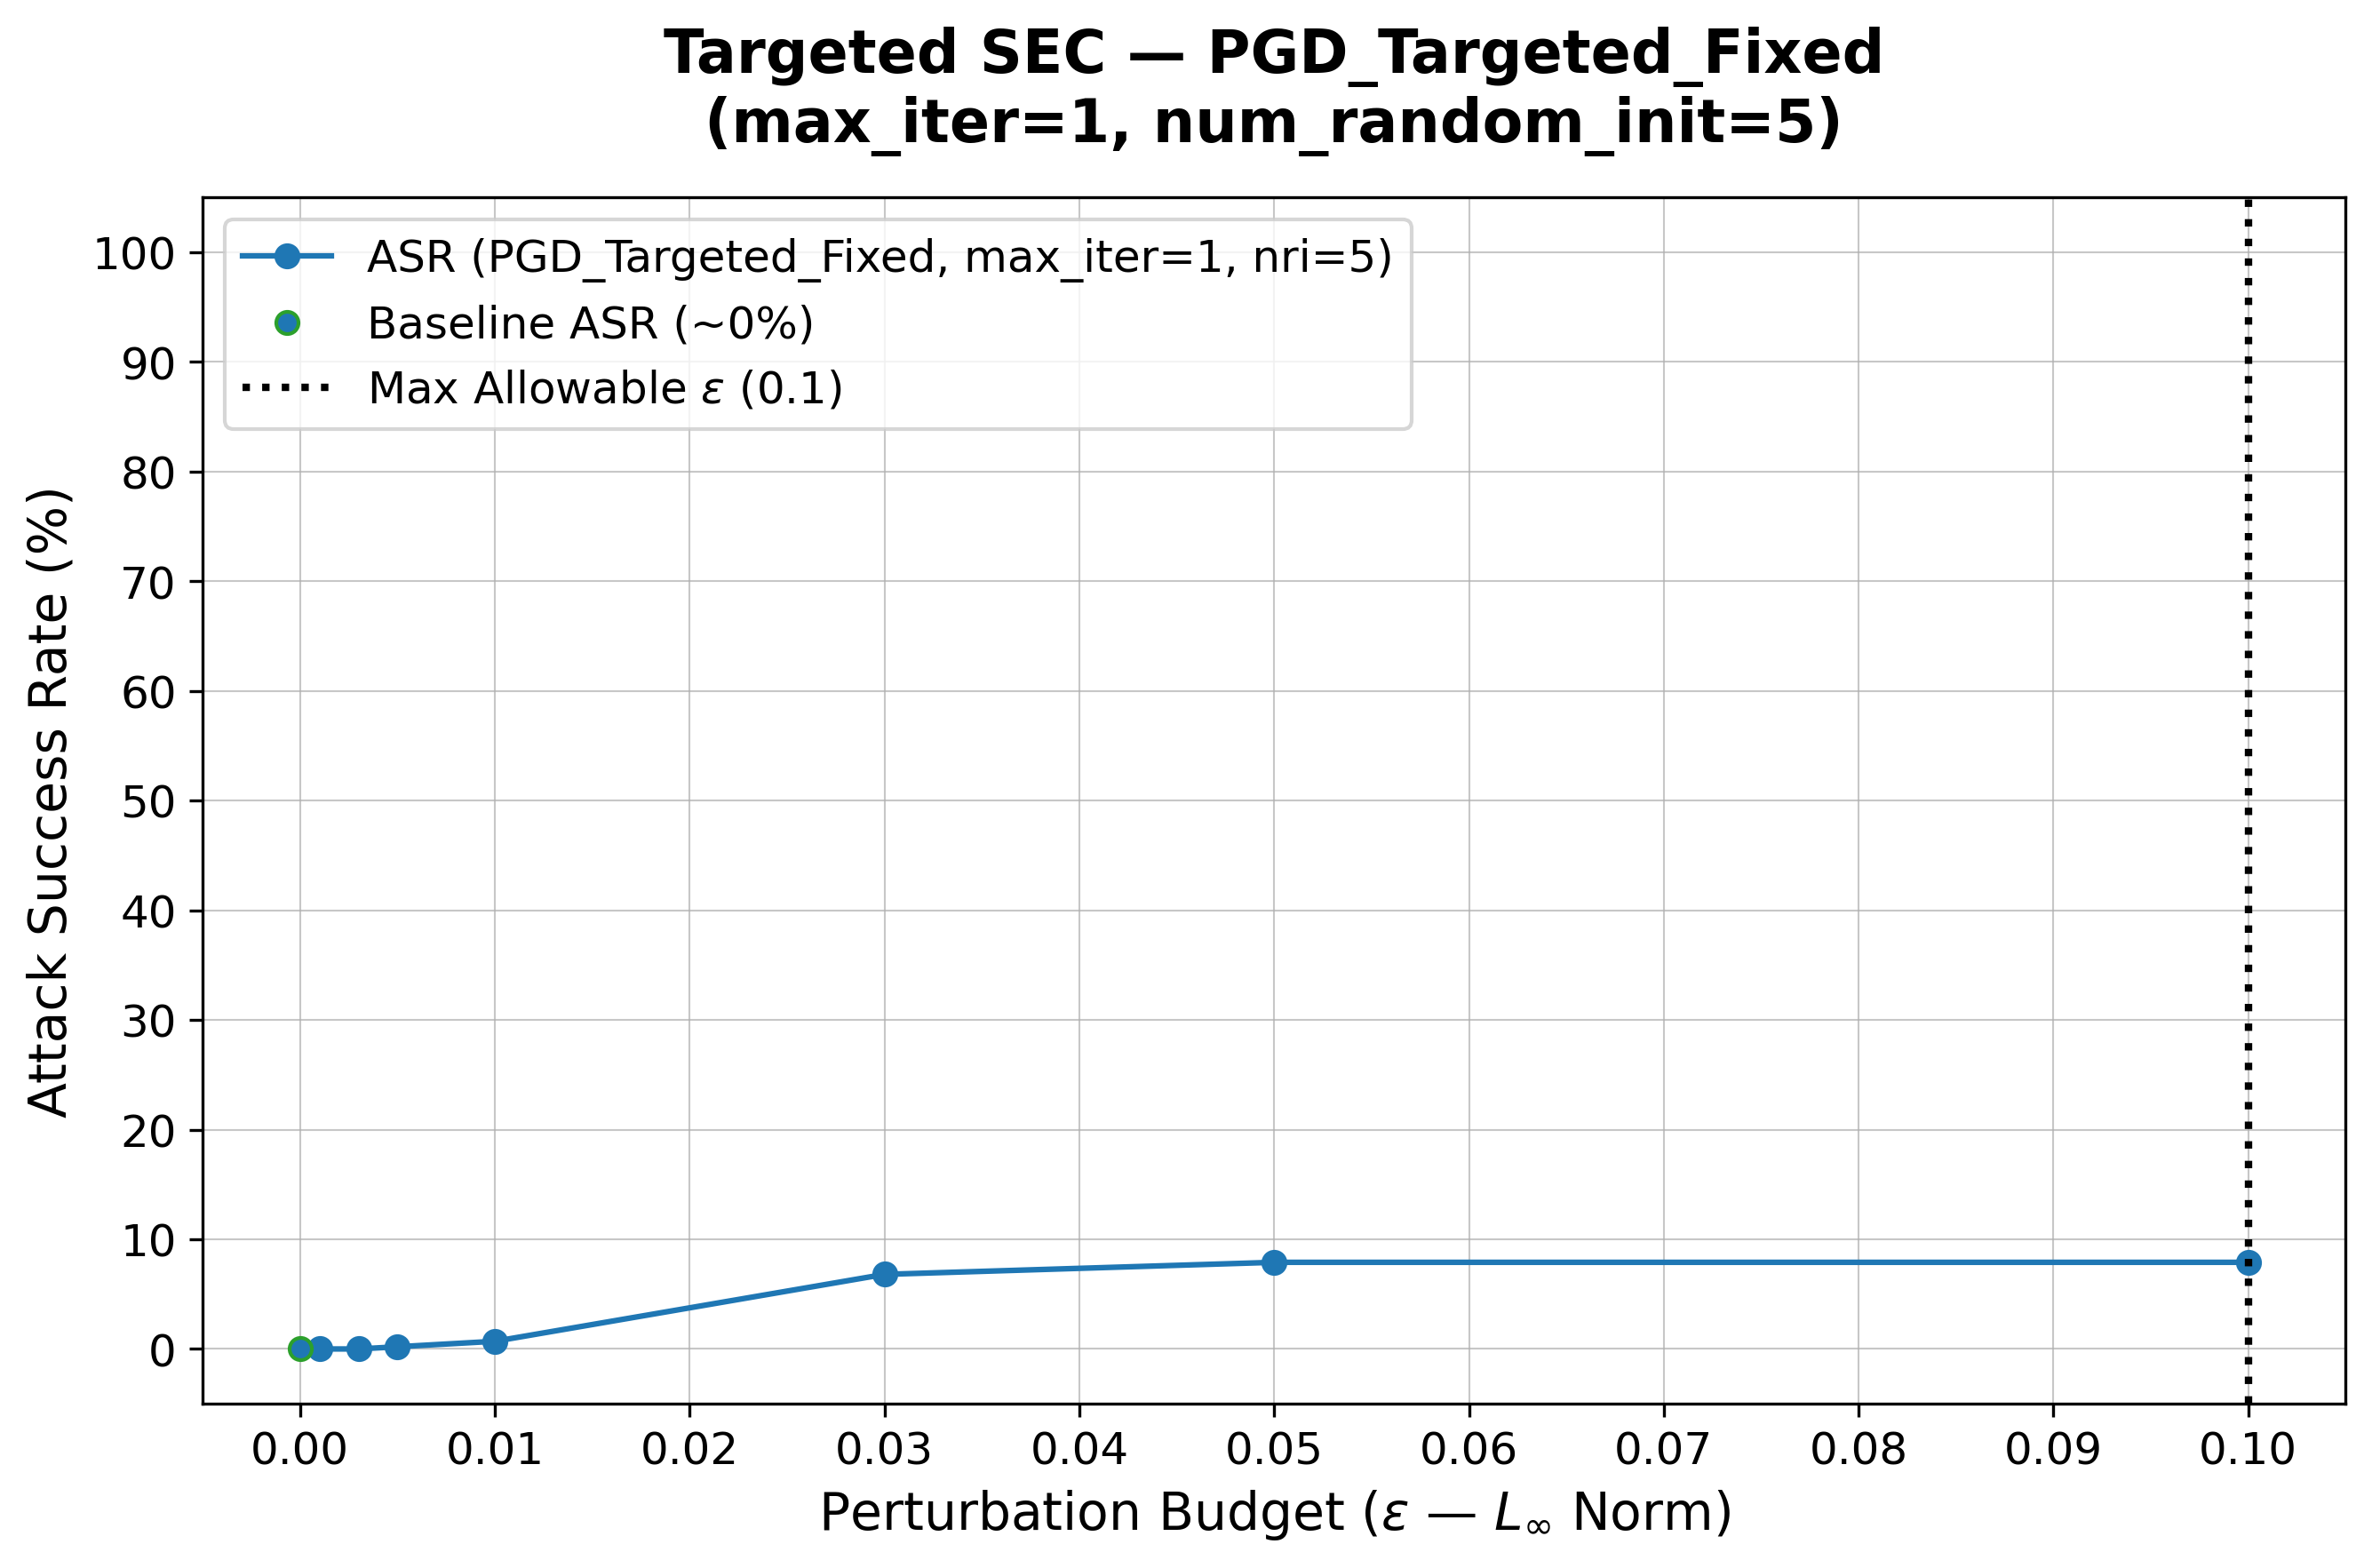
\includegraphics[width=\textwidth]{PGD_Error_specific/Fixed/PGD_Targeted_Fixed_nri5_iter1_SEC.png}
        \caption{\texttt{max_iter} = 1}
        \label{fig:PGD_nri5_iter1}
    \end{subfigure}
    \hfill
    % Sotto-figura 2
    \begin{subfigure}[b]{0.45\textwidth}
        \centering
        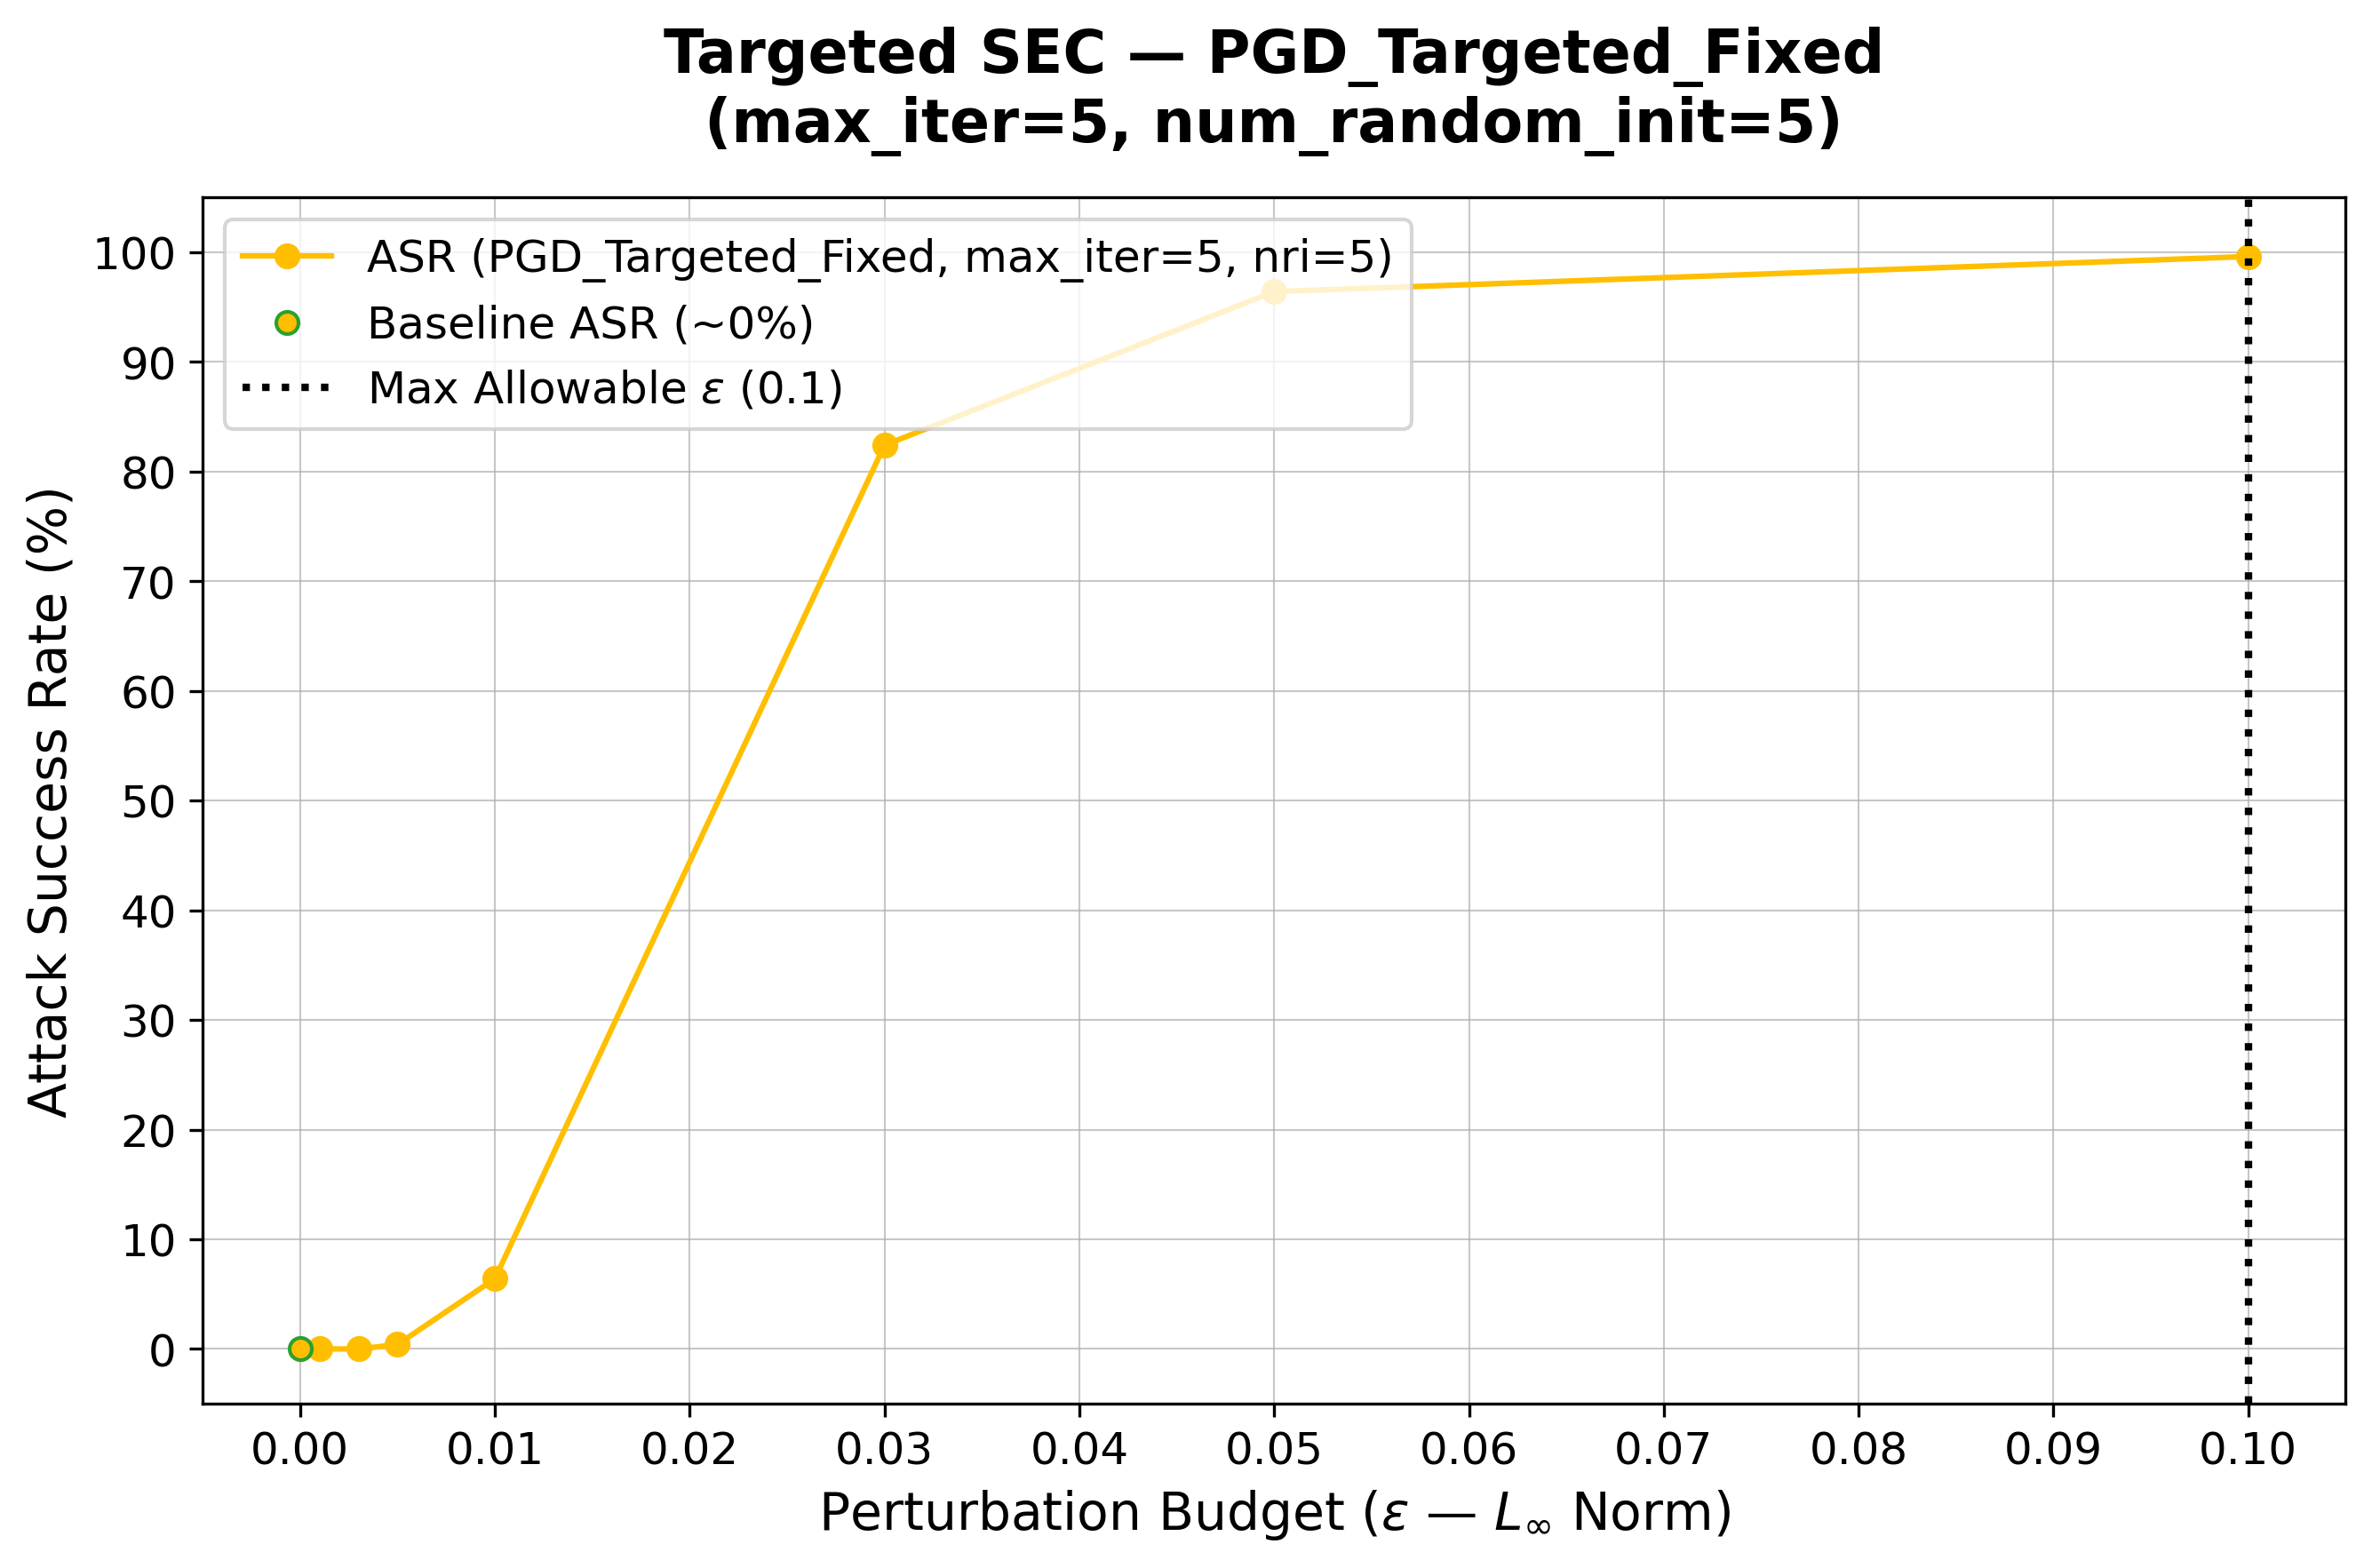
\includegraphics[width=\textwidth]{PGD_Error_specific/Fixed/PGD_Targeted_Fixed_nri5_iter5_SEC.png}
        \caption{\texttt{max_iter} = 5}
        \label{fig:PGD_nri5_iter5}
    \end{subfigure}

    \vspace{1em} % Spazio verticale tra le righe di immagini
    % Sotto-figura 3
    \begin{subfigure}[b]{0.45\textwidth}
        \centering
        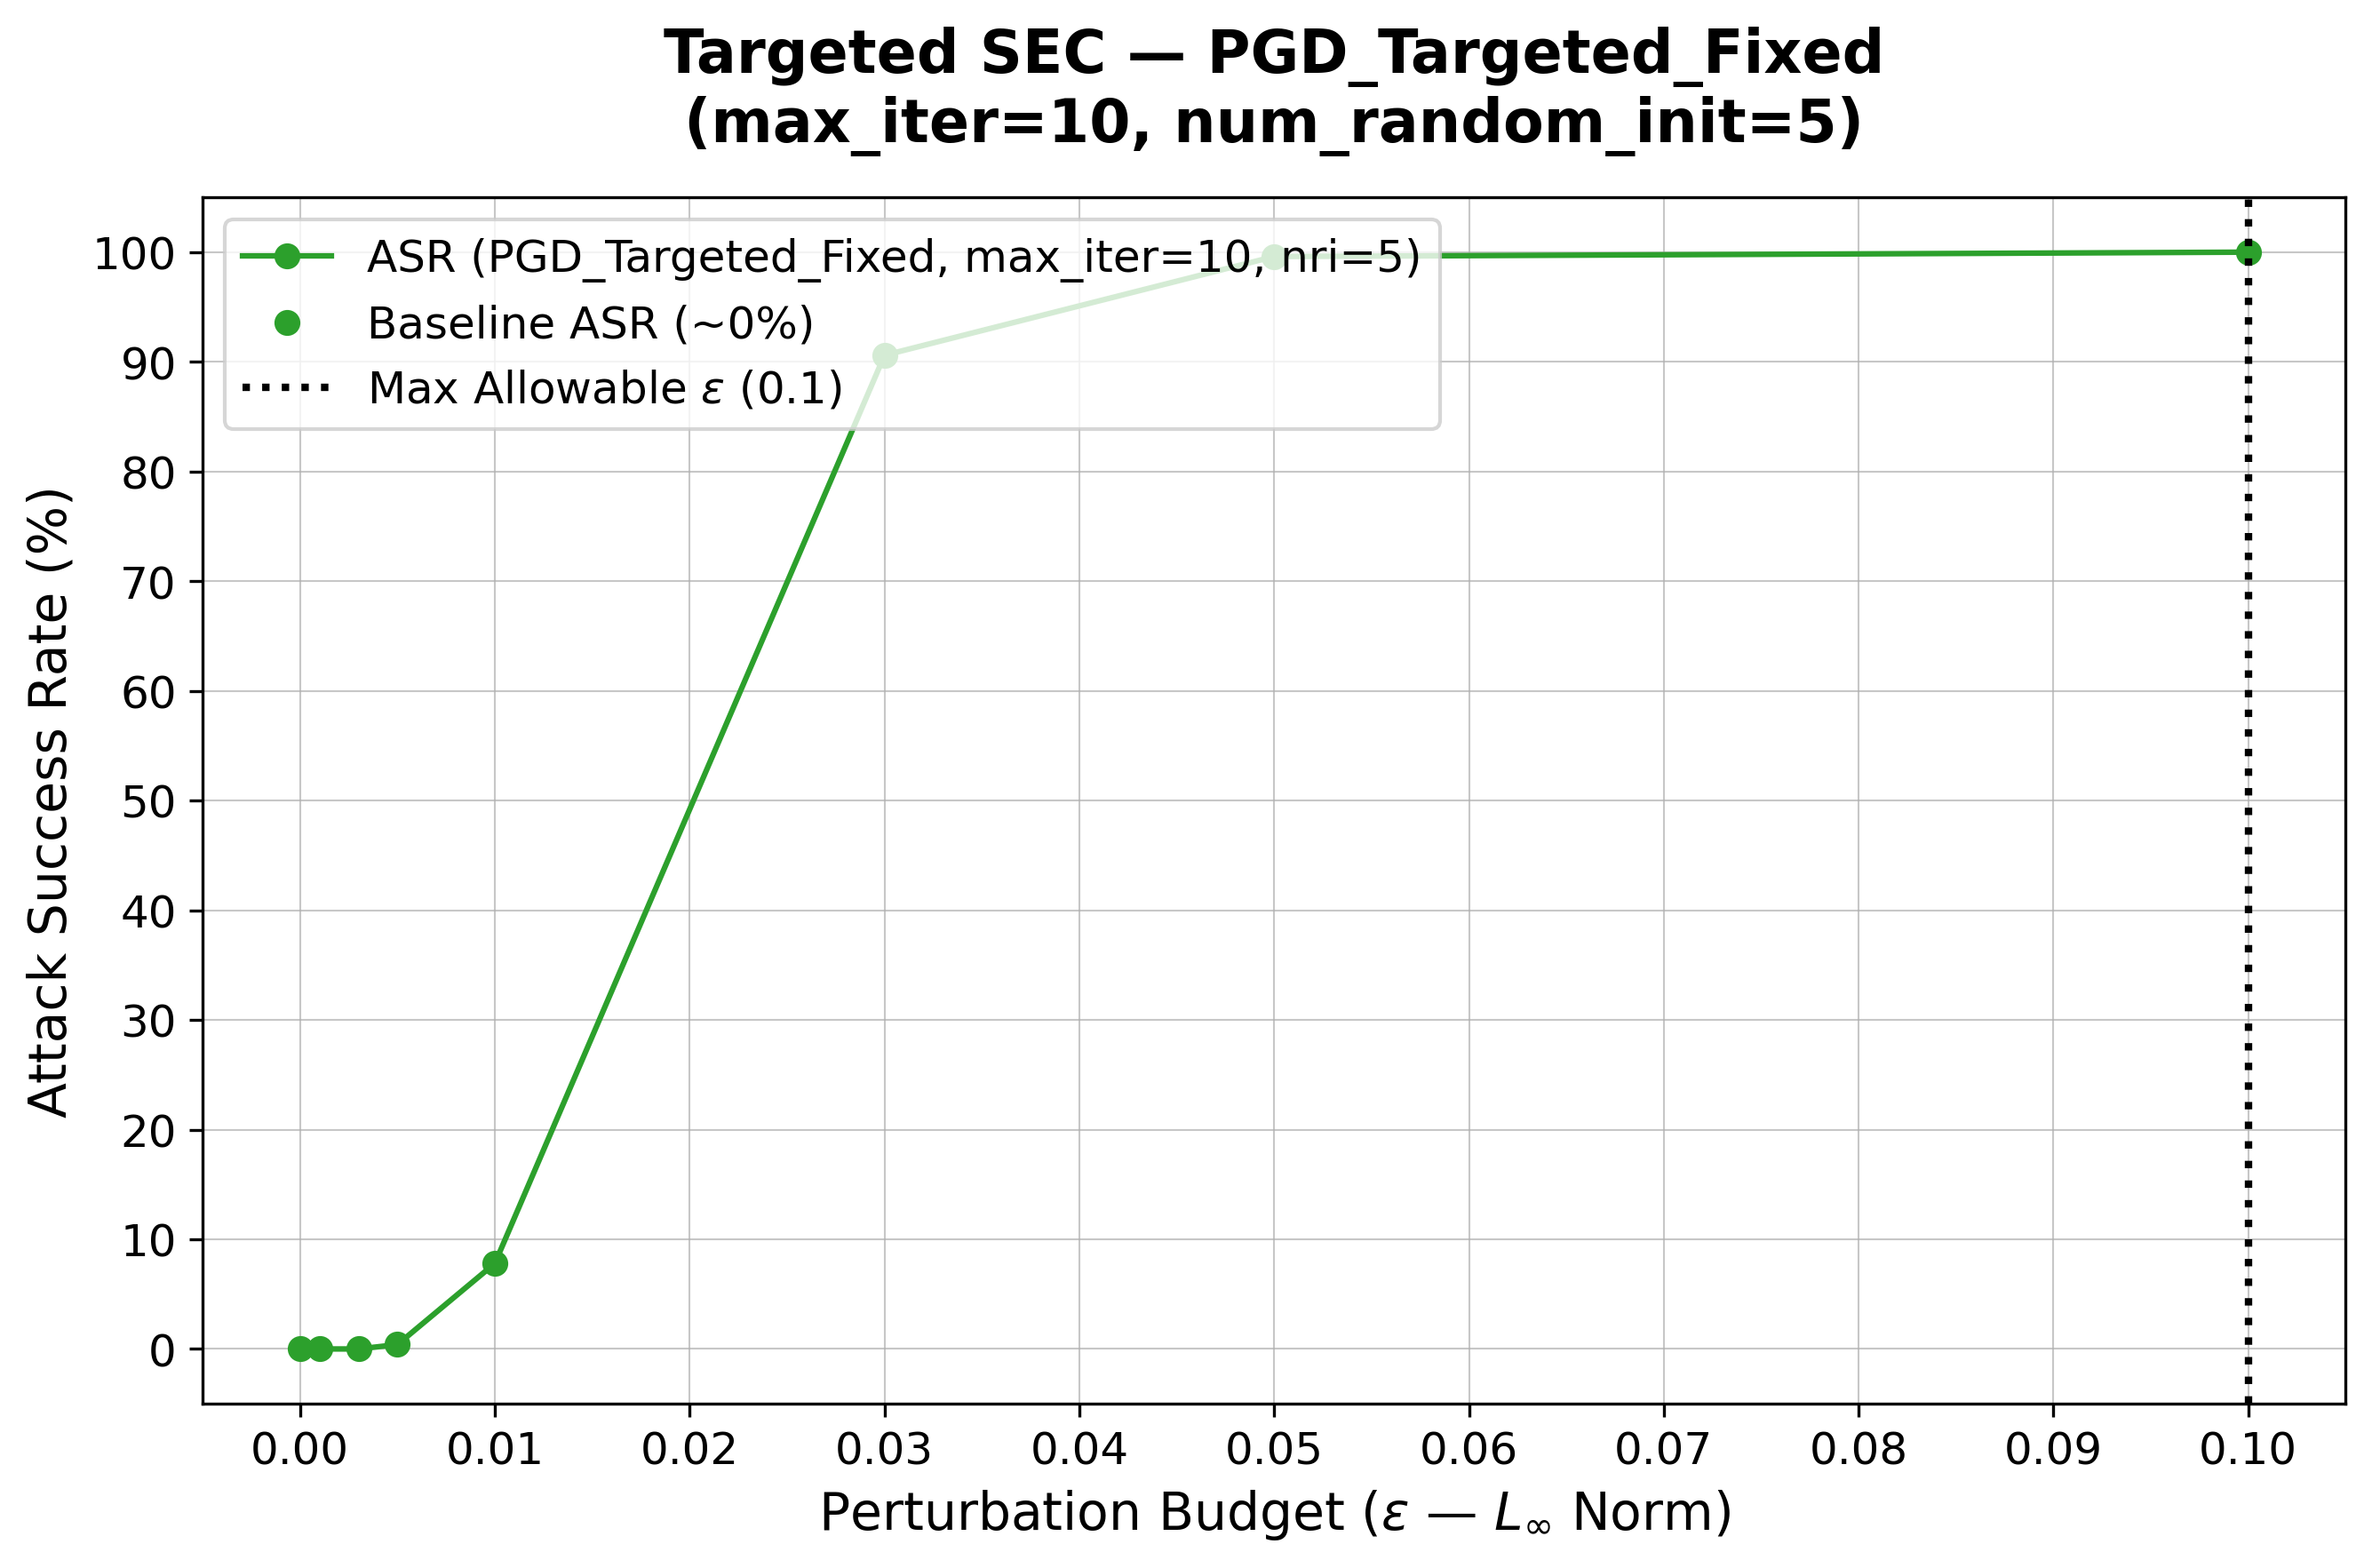
\includegraphics[width=\textwidth]{PGD_Error_specific/Fixed/PGD_Targeted_Fixed_nri5_iter10_SEC.png}
        \caption{\texttt{max_iter} = 10}
        \label{fig:PGD_nri5_iter10}
    \end{subfigure}
    \hfill
    % Sotto-figura 4
    \begin{subfigure}[b]{0.45\textwidth}
        \centering
        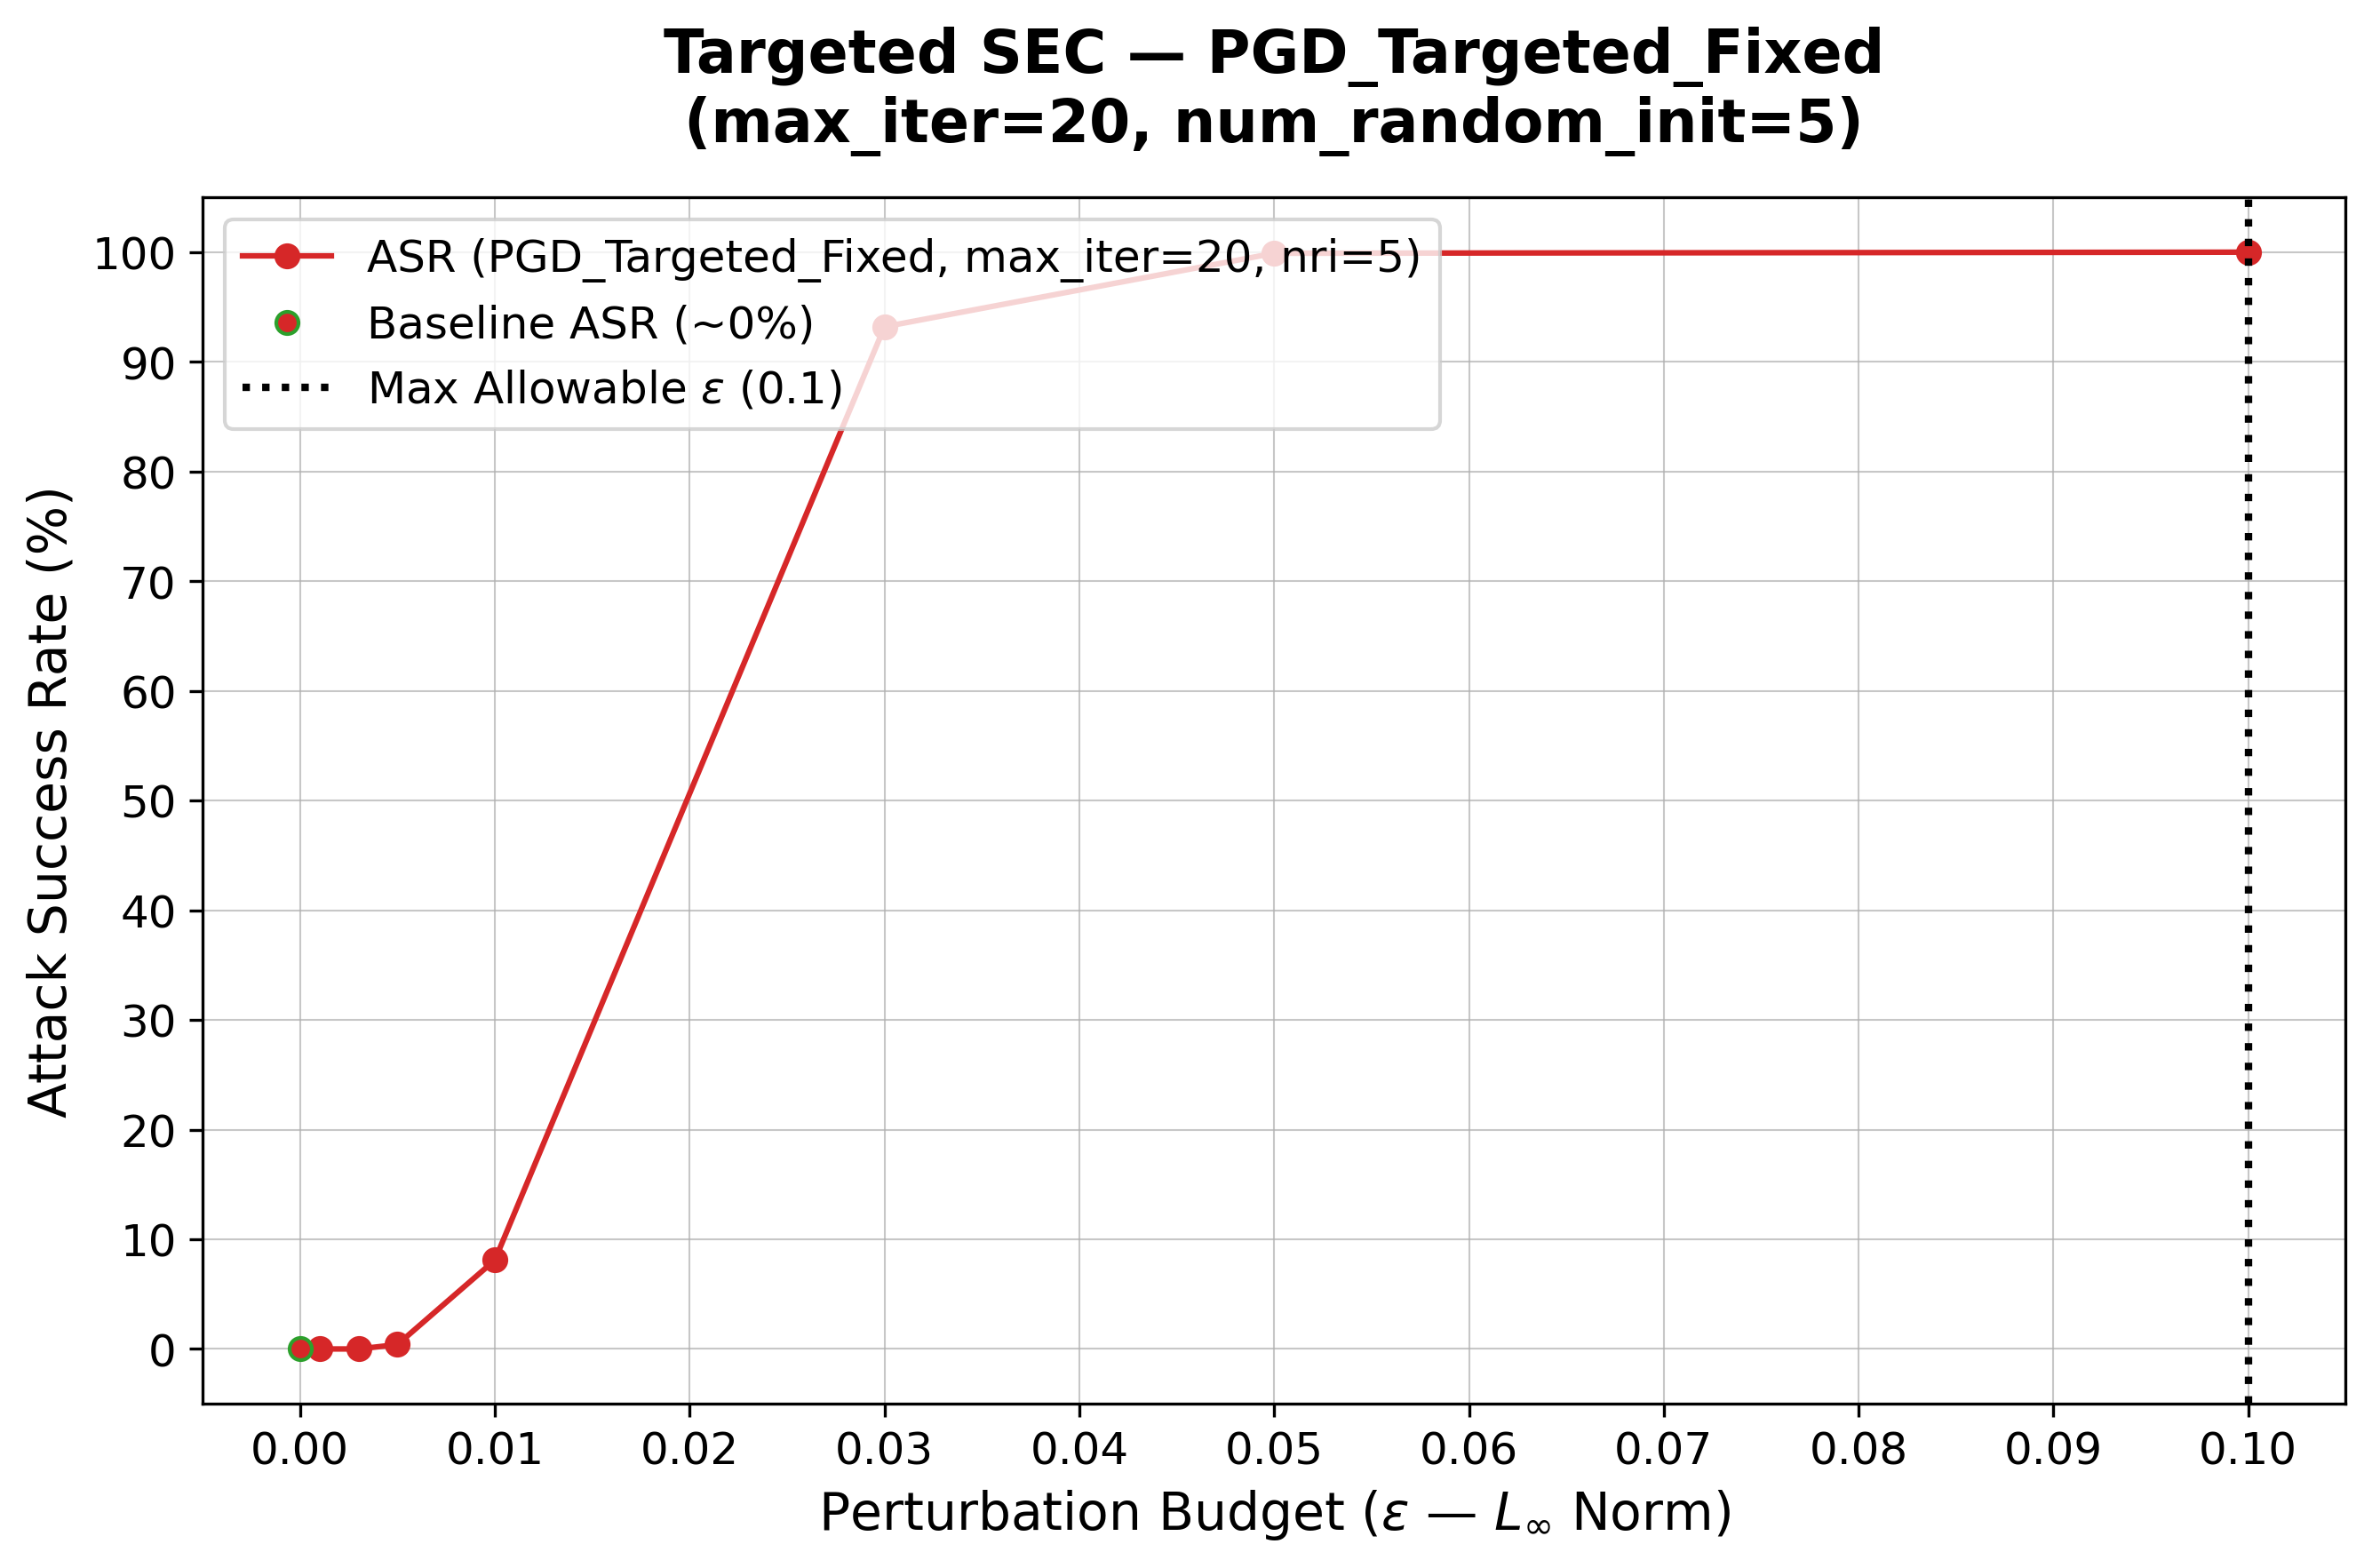
\includegraphics[width=\textwidth]{PGD_Error_specific/Fixed/PGD_Targeted_Fixed_nri5_iter20_SEC.png}
        \caption{\texttt{max_iter} = 20}
        \label{fig:PGD_nri5_iter20}
    \end{subfigure}
    \vspace{1em} % Spazio verticale tra le righe di immagini
    % Sotto-figura 5
    \begin{subfigure}[b]{0.45\textwidth}
        \centering
        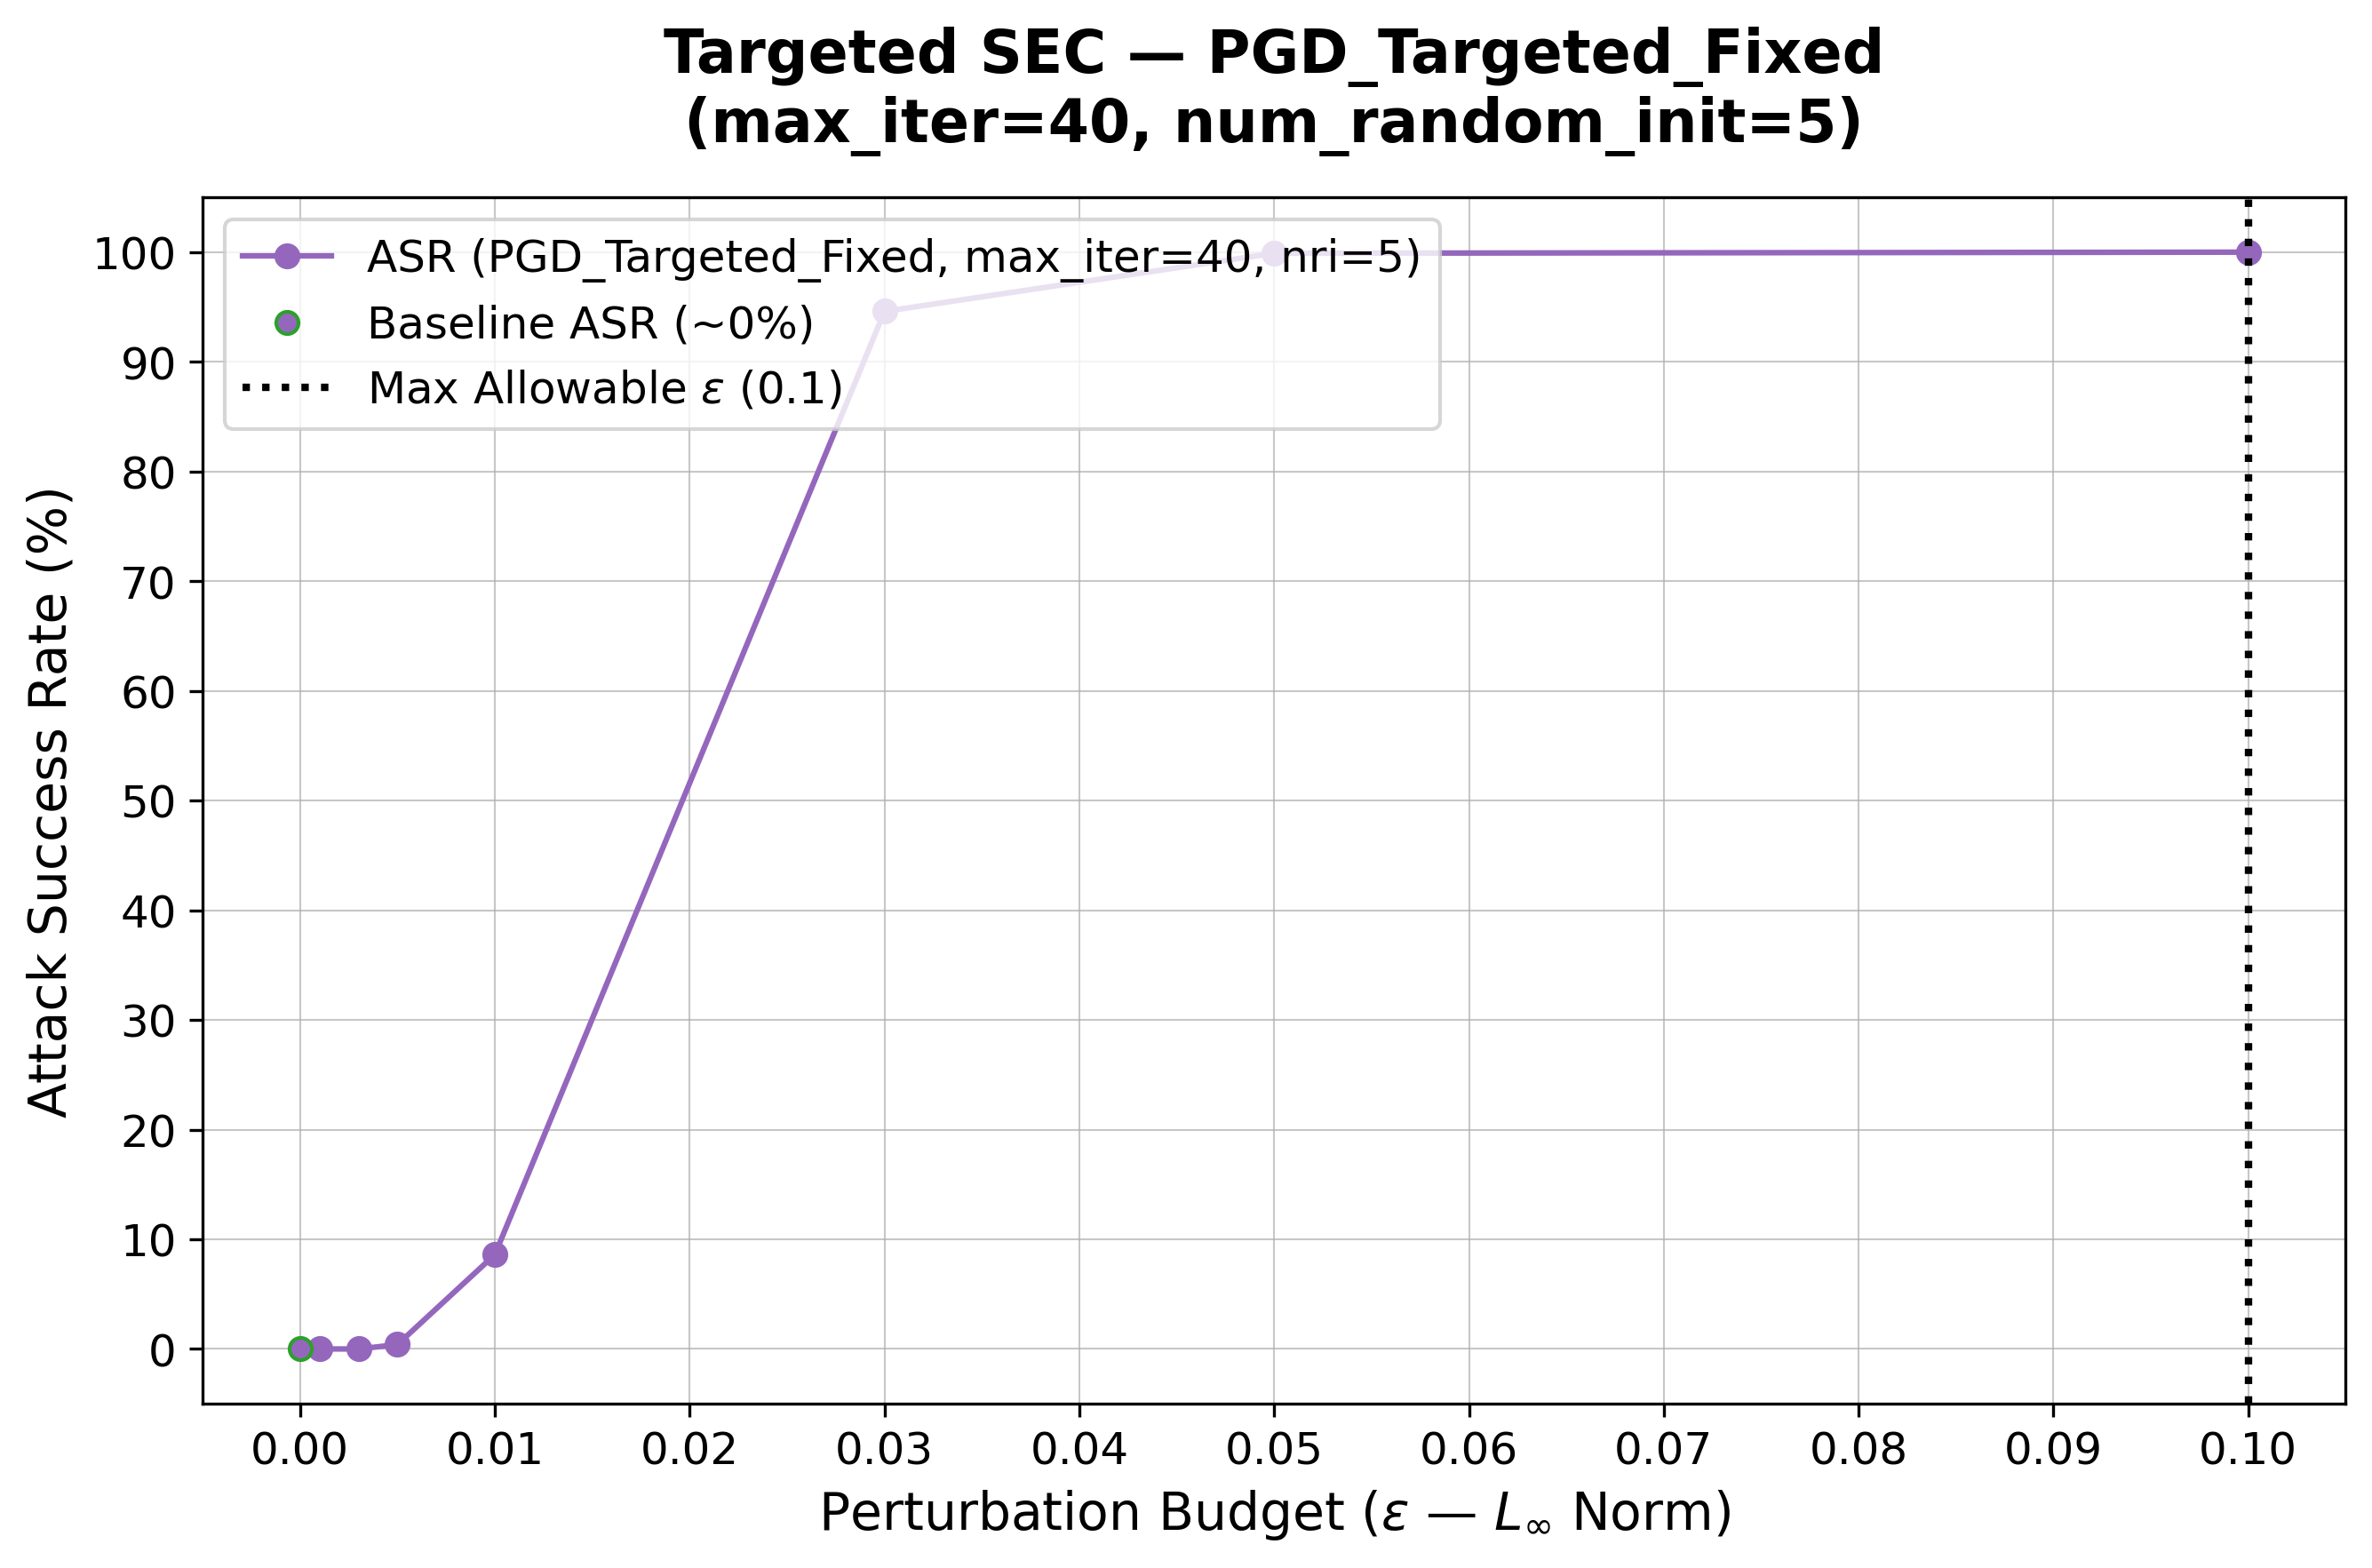
\includegraphics[width=\textwidth]{PGD_Error_specific/Fixed/PGD_Targeted_Fixed_nri5_iter40_SEC.png}
        \caption{\texttt{max_iter} = 40}
        \label{fig:PGD_nri5_iter40}
    \end{subfigure}
    \caption{PGD Fixed - Iterazioni a confronto per \texttt{nri} = 5}
    \label{fig:PGD_iterations_nri5}
\end{figure}

% -- GRAFICO COMPARATIVO PER VARI NRI E MAX ITER--
\begin{figure}[H]
    \centering
    
    % Il \makebox centrato sulla larghezza del testo garantisce la simmetria perfetta
    \makebox[\textwidth][c]{
        \begin{tabular}{cc}
            
            % Sotto-figura 1 (Sinistra, Riga 1)
            \begin{subfigure}[b]{0.55\textwidth}
                \centering
                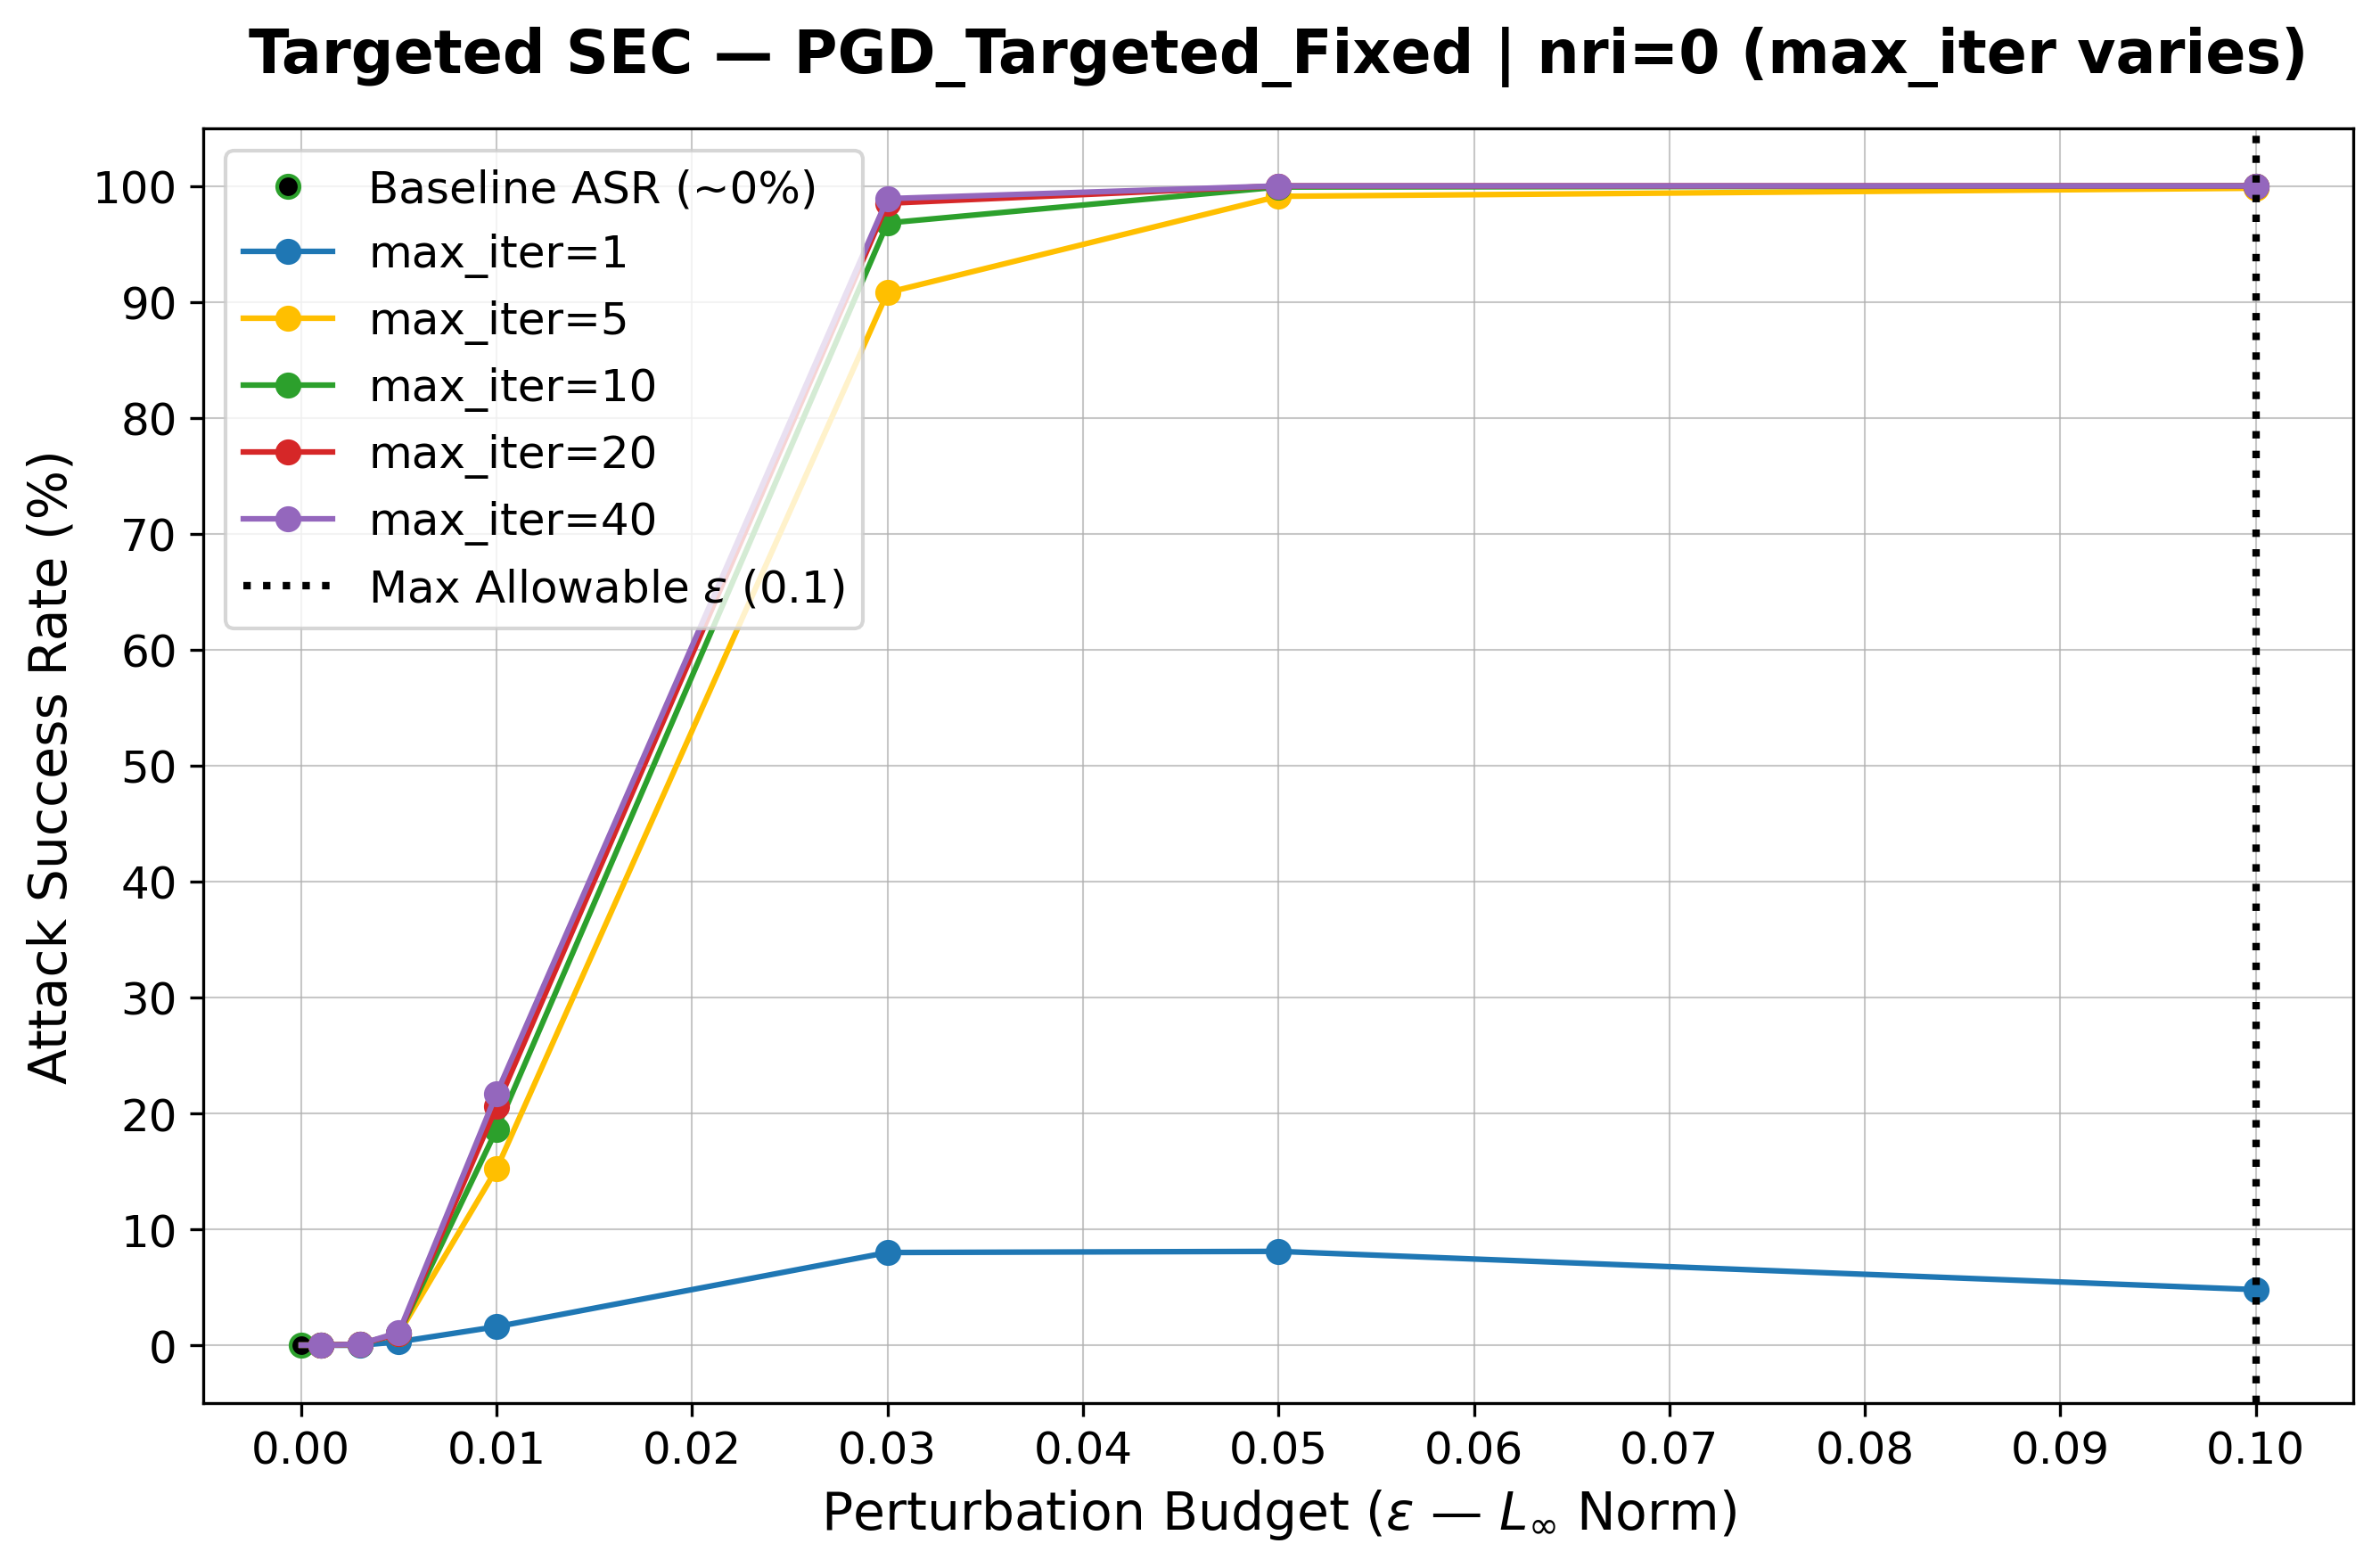
\includegraphics[width=\textwidth]{PGD_Error_specific/Fixed/PGD_Targeted_Fixed_nri0_comparative_maxiter_SEC.png}
                \caption{PGD SEC con \texttt{nri} = 0}
                \label{fig:PGD_nri0_vari_iter}
            \end{subfigure}
            &
            % Sotto-figura 2 (Destra, Riga 1)
            \begin{subfigure}[b]{0.55\textwidth}
                \centering
                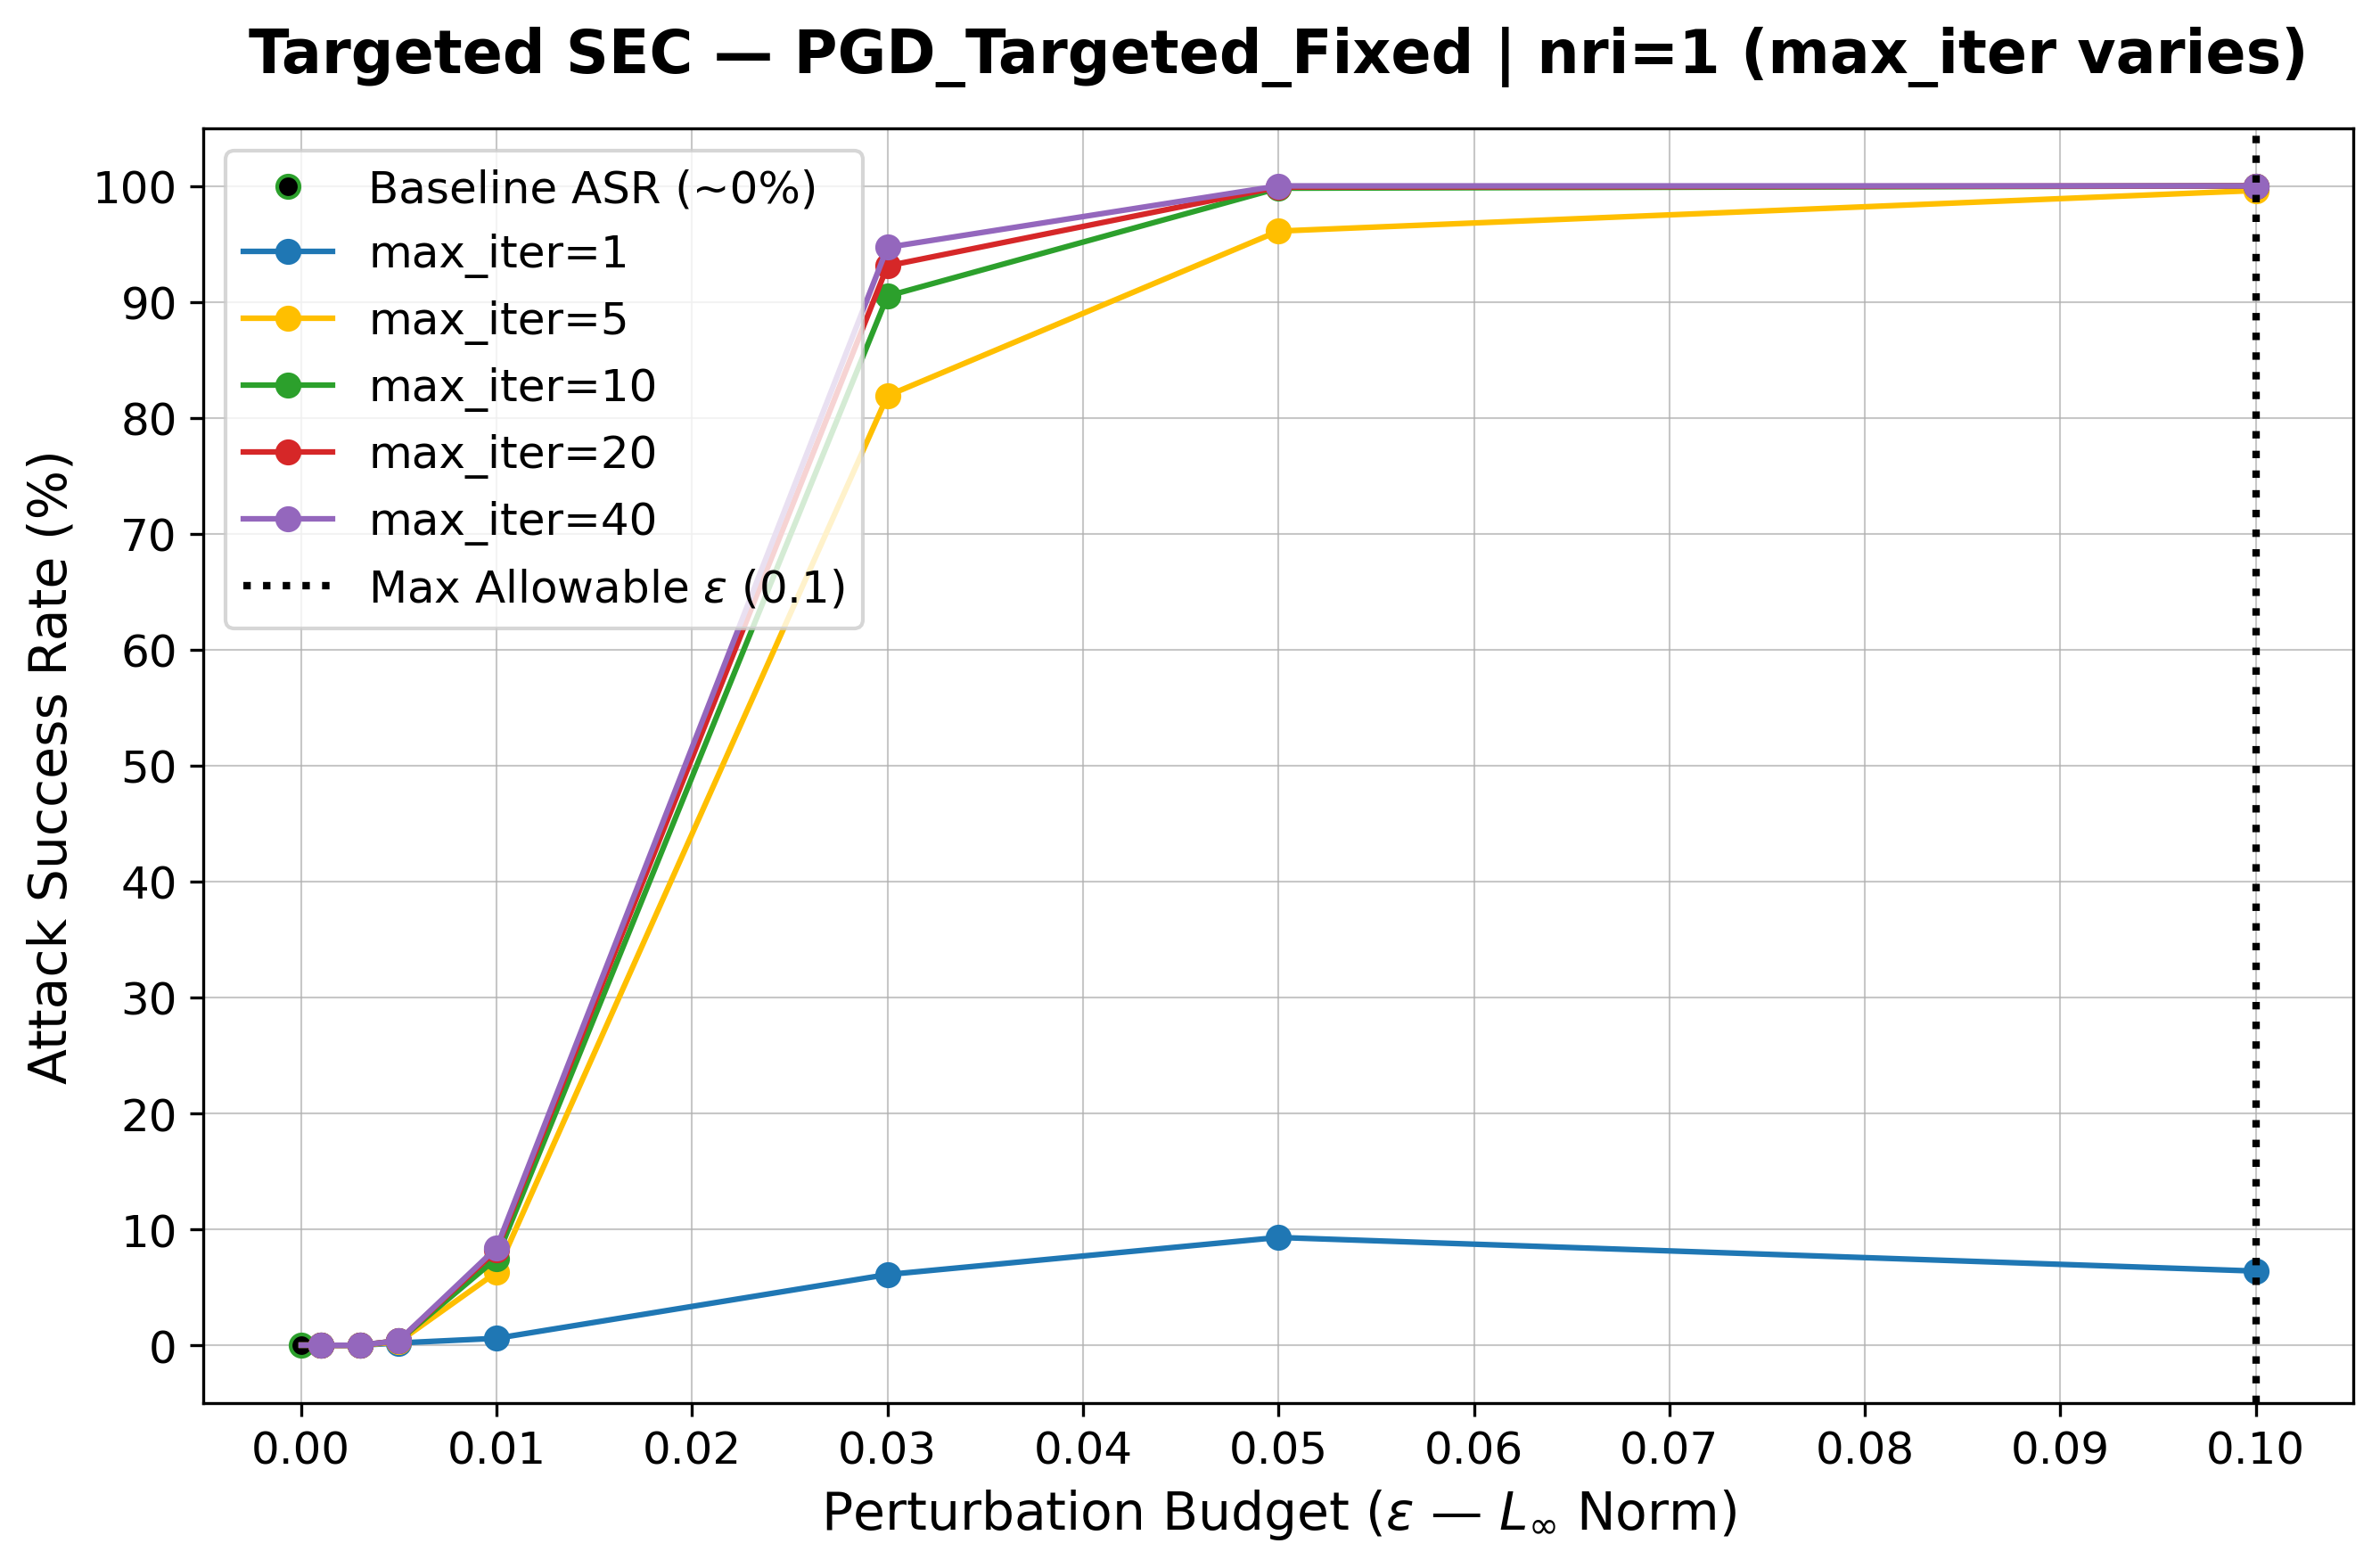
\includegraphics[width=\textwidth]{PGD_Error_specific/Fixed/PGD_Targeted_Fixed_nri1_comparative_maxiter_SEC.png}
                \caption{PGD SEC con \texttt{nri} = 1}
                \label{fig:PGD_nri1_vari_iter}
            \end{subfigure} \\ [1em] % Spazio verticale tra le righe
            
            % Sotto-figura 3 (Sinistra, Riga 2)
            \begin{subfigure}[b]{0.55\textwidth}
                \centering
                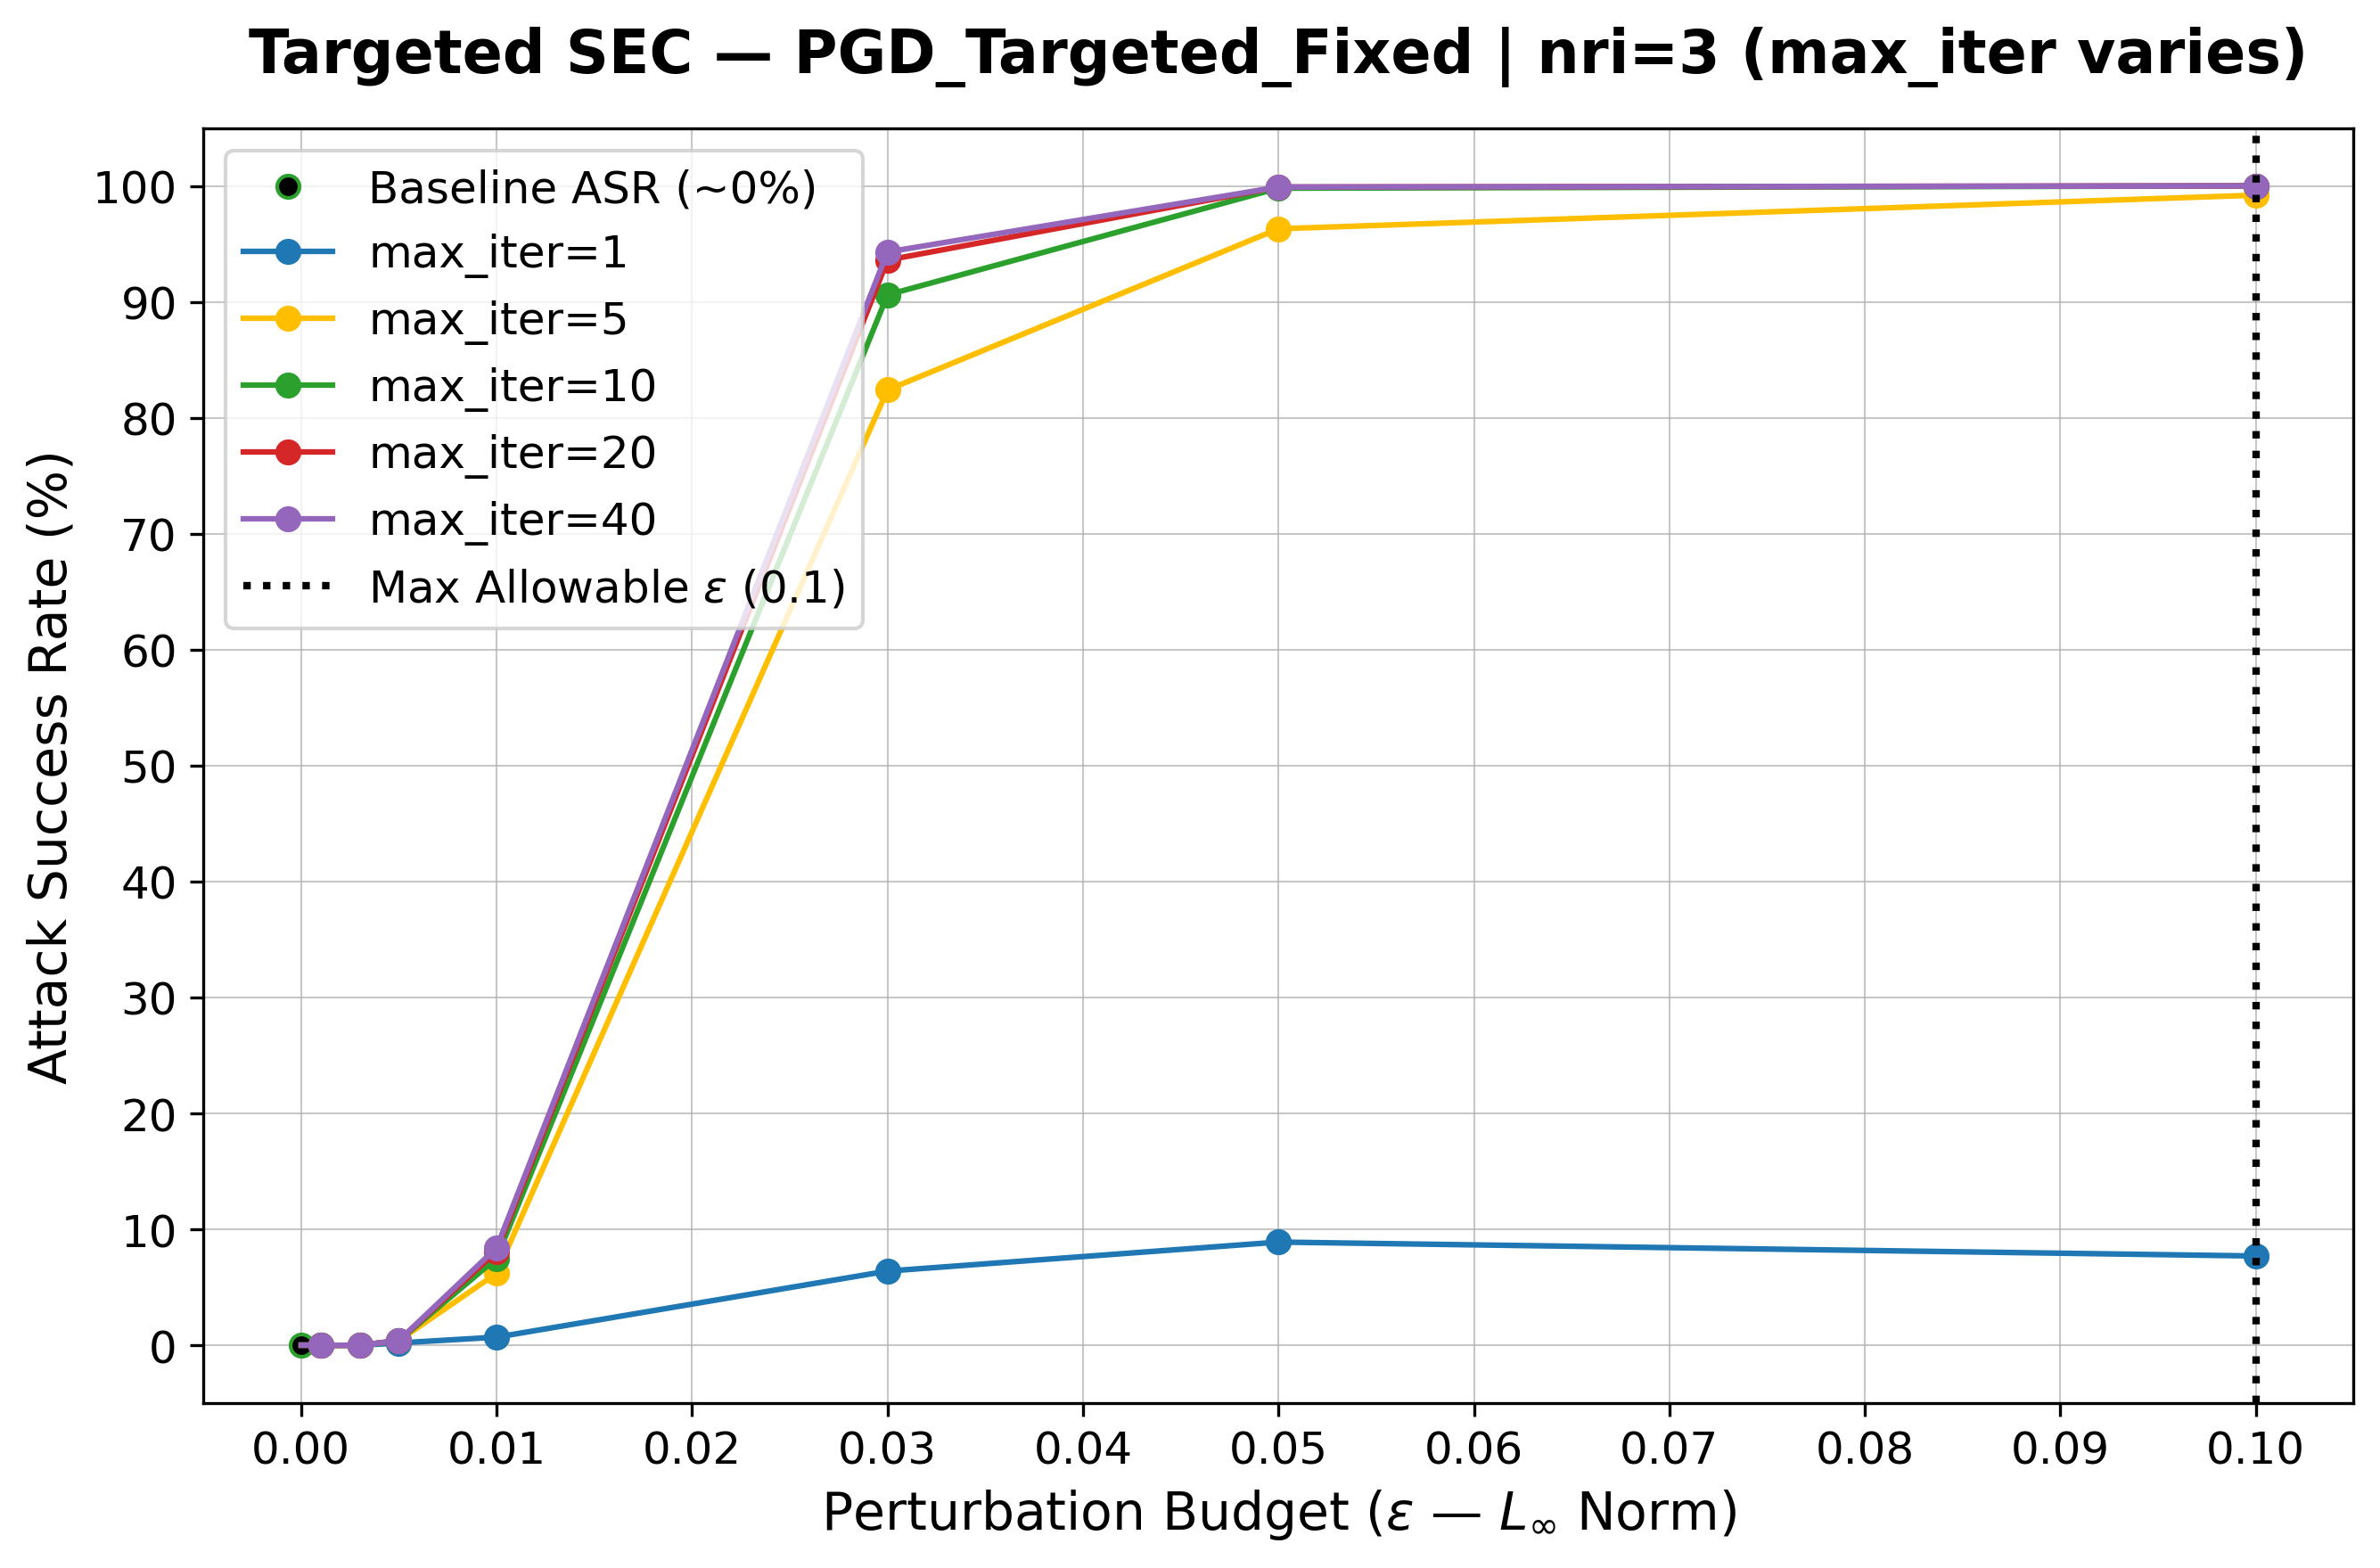
\includegraphics[width=\textwidth]{PGD_Error_specific/Fixed/PGD_Targeted_Fixed_nri3_comparative_maxiter_SEC.png}
                \caption{PGD SEC con \texttt{nri} = 3}
                \label{fig:PGD_nri3_vari_iter}
            \end{subfigure}
            &
            % Sotto-figura 4 (Destra, Riga 2)
            \begin{subfigure}[b]{0.55\textwidth}
                \centering
                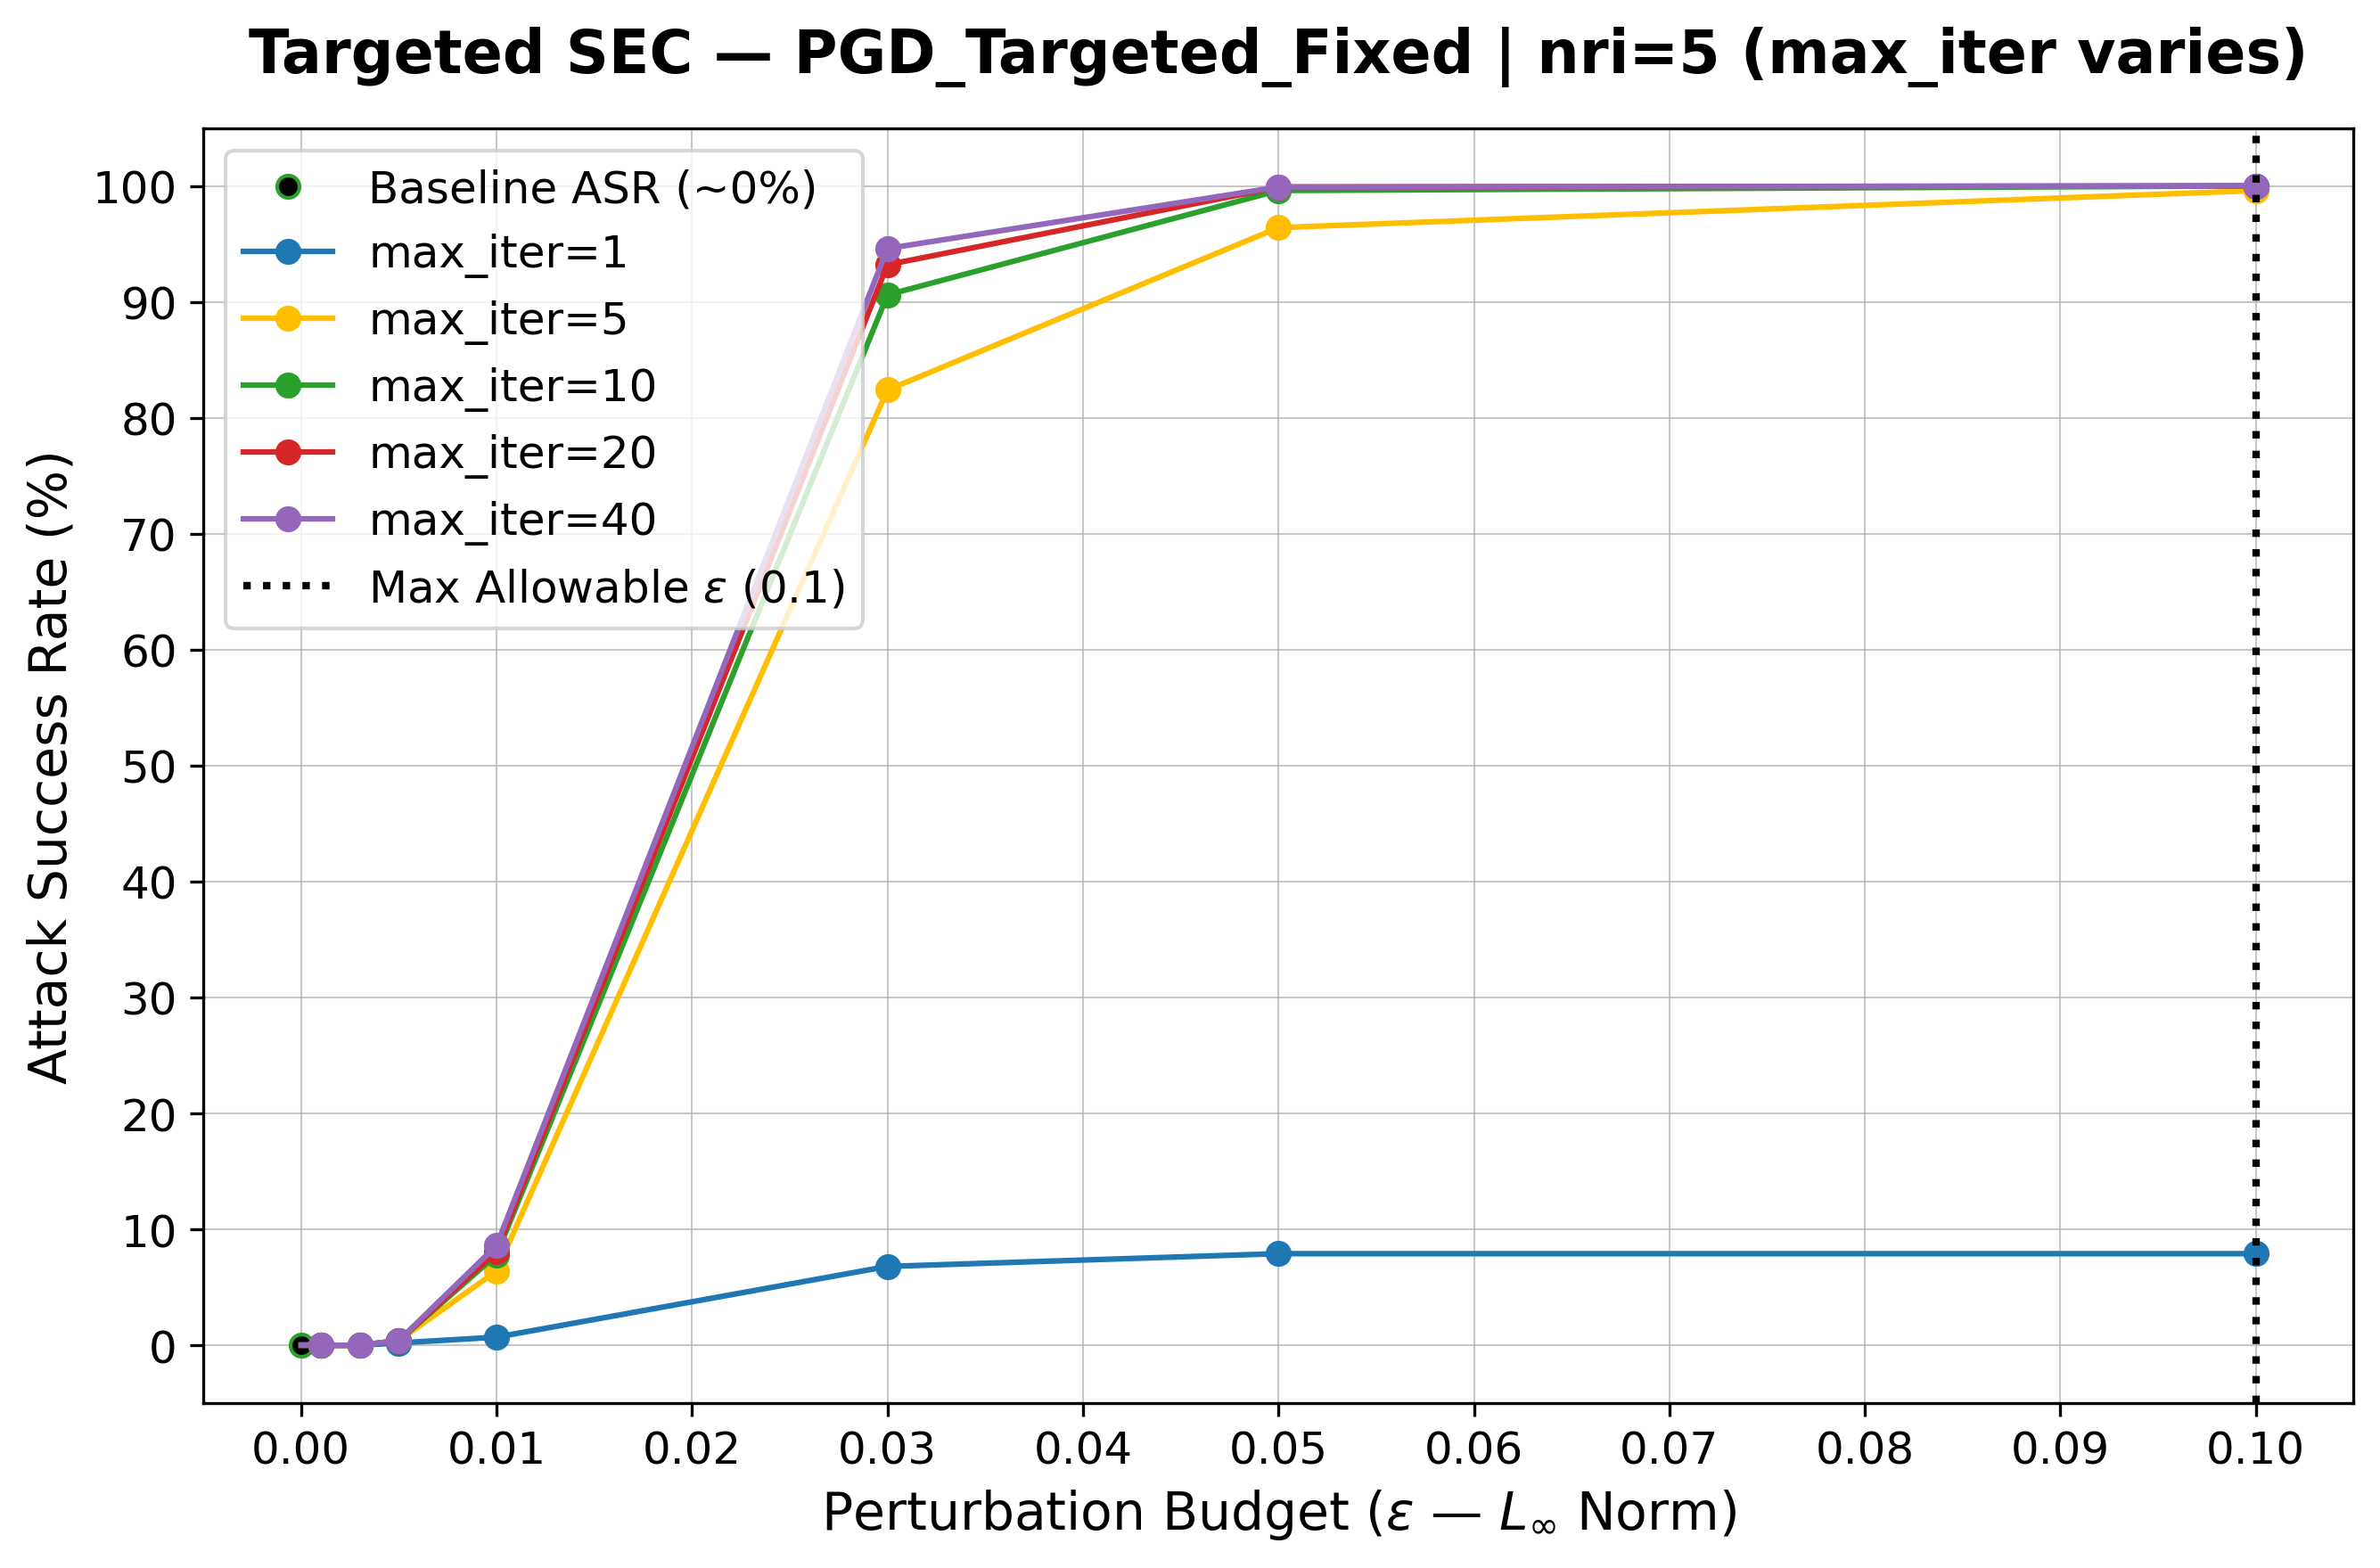
\includegraphics[width=\textwidth]{PGD_Error_specific/Fixed/PGD_Targeted_Fixed_nri5_comparative_maxiter_SEC.png}
                \caption{PGD SEC con \texttt{nri} = 5}
                \label{fig:PGD_nri5_vari_iter}
            \end{subfigure}
            
        \end{tabular}
    }
    
    \caption{PGD - Iterazioni a confronto per vari \texttt{nri}}
    \label{fig:PGD_iterations_vari_nri}
\end{figure}

Quest ultimo set di grafici evidenzia in modo chiaro anche la poca influenza del paramentro \texttt{num\_random\_init} sull'efficacia complessiva dell'attacco. A parità di iterazioni e \textit{budget}, l'ASR rimane sostanzialmente invariato al variare del numero di riavvii casuali, confermando che, per un attacco a bersaglio fisso, la componente stocastica non apporta alcun beneficio in termini di successo offensivo.

\clearpage
\subsubsection*{Least Likely Attack}
In questo scenario estremo, l'intuizione matematica suggerirebbe che i \textit{random restart} forniscano un vantaggio cruciale, permettendo all'ottimizzatore di esplorare traiettorie di attacco alternative.

Tuttavia, i risultati empirici estratti dalla \textit{grid search} smentiscono questa assunzione, confermando l'osservazione nella modalità \textit{Fixed}. L'introduzione dei riavvii casuali non solo non migliora l'attacco, ma cala l'efficacia offensiva. 

Analizzando i dati tabellari per un numero solido di iterazioni (\texttt{max\_iter} = 20) in una fascia di \textit{budget} intermedio ($\epsilon = 0.03$), la configurazione puramente deterministica (\texttt{nri} = 0, equivalente a BIM) riesce a forzare l'inganno nel 75.1\% dei casi. Attivando 5 \textit{random restart}, l'\textit{Attack Success Rate} (ASR) cala al 55.6\%. La medesima dinamica di degrado si osserva a $\epsilon = 0.05$ (l'ASR scende dal 99.2\% al 96.7\%) e riducendo il parametro iterativo (a \texttt{max\_iter} = 10 e $\epsilon = 0.03$, l'ASR passa dal 65.6\% della variante $nri = 0$ al 44.6\% della variante con 5 riavvii). 

La giustificazione geometrica di questo fallimento risiede nella rigorosa limitazione imposta dal \textit{budget} in norma $L_\infty$. Per raggiungere la classe \textit{Least Likely}, l'immagine deve coprire una distanza enorme. L'approccio deterministico sfrutta il 100\% del \textit{budget} disponibile muovendosi lungo il vettore ottimale calcolato sin dal primo step. Al contrario, PGD impiega il primo sbalzo perturbativo per muoversi in una direzione casuale. Dopo aver esguito questo salto alla cieca, il budget a disposizione rischia di non essere abbastanza ampio per correggere la traiettoria e raggiungere la regione decisionale opposta a quella della ground truth, soprattutto quando il numero di iterazioni è limitato.

Dal punto di vista dell'efficienza elaborativa, il bilancio è ulteriormente aggravato. Eseguire l'attacco estremo con \texttt{max\_iter} = 40 e \texttt{nri} = 5 ha richiesto circa 770 secondi (rispetto ai 123 secondi dell'esecuzione deterministica), restituendo peraltro performance sistematicamente inferiori o tuttalpiù identiche in regime di saturazione ($\epsilon=0.1$).

In conclusione, questa disamina empirica dimostra che, se vincolati a un \textit{budget} rigido e ad una limitata potenza computazionale, gli algoritmi basati sul segno del gradiente operano al massimo della loro efficienza quando guidati da una discesa pura e ininterrotta (BIM).
In tabella~\ref{tab:PGD_least_likely}, è sintetizzata in maniera compatta l'analisi quantitativa discussa in precedenza relativa all'attacco. Al fine di esaminare nel dettaglio l'impatto degli iperparametri di PGD su bersagli semanticamente remoti, sono stati prodotti molteplici grafici comparativi. Ciascuna visualizzazione principale è corredata da sotto-grafici dedicati, progettati per isolare e rendere maggiormente leggibili le singole curve di interesse (al variare di \texttt{num\_random\_init} e \texttt{max\_iter}).

Inoltre, per agevolare una valutazione visiva immediata dell'efficacia algoritmica, in Figura~\ref{fig:PGD_LL_iterations_vari_nri} è presentata una matrice di immagini che affianca le \textit{Security Evaluation Curve} (SEC) comparative. Questa struttura matriciale illustra l'evoluzione dell'\textit{Attack Success Rate} al variare della profondità iterativa (\texttt{max\_iter} $\in \{1, 5, 10, 20, 40\}$) esplorando tutte le configurazioni (\texttt{num\_random\_init}) analizzate nel test.

\begin{table}[H]
    \centering
    \begin{tabular}{ccccc}
    \toprule
        \textbf{nri} & \textbf{max_iter} & $\boldsymbol{\epsilon}$ & \textbf{ASR (\%)} & \textbf{Time (s)} \\
        \midrule
        0 & 20 & 0.001 & 0.0 & 70.01\\
        0 & 20 & 0.003 & 0.0 & 70.34\\
        0 & 20 & 0.005 & 0.0 & 116.94\\
        0 & 20 & 0.01 & 0.3 & 69.42\\
        \textbf{0} & \textbf{20} & \textbf{0.03} & \textbf{75.1} & \textbf{67.71}\\
        0 & 20 & 0.05 & 99.2 & 114.05\\
        0 & 20 & 0.1 & 100.0 & 65.97\\
        5 & 20 & 0.001 & 0.0 & 354.07\\
        5 & 20 & 0.003 & 0.0 & 402.85\\
        5 & 20 & 0.005 & 0.0 & 400.45\\
        5 & 20 & 0.01 & 0.2 & 399.78\\
        5 & 20 & 0.03 & 55.6 & 349.09\\
        5 & 20 & 0.05 & 96.7 & 394.92\\
        5 & 20 & 0.1 & 100.0 & 396.02\\
    \bottomrule
    \end{tabular}
    \caption{Vista ridotta per l'analisi quantitativa di PGD Least Likely}
    \label{tab:PGD_least_likely}
\end{table}

\clearpage
% -- SEC NRI = 0 --
\begin{figure}[H]
    \centering
    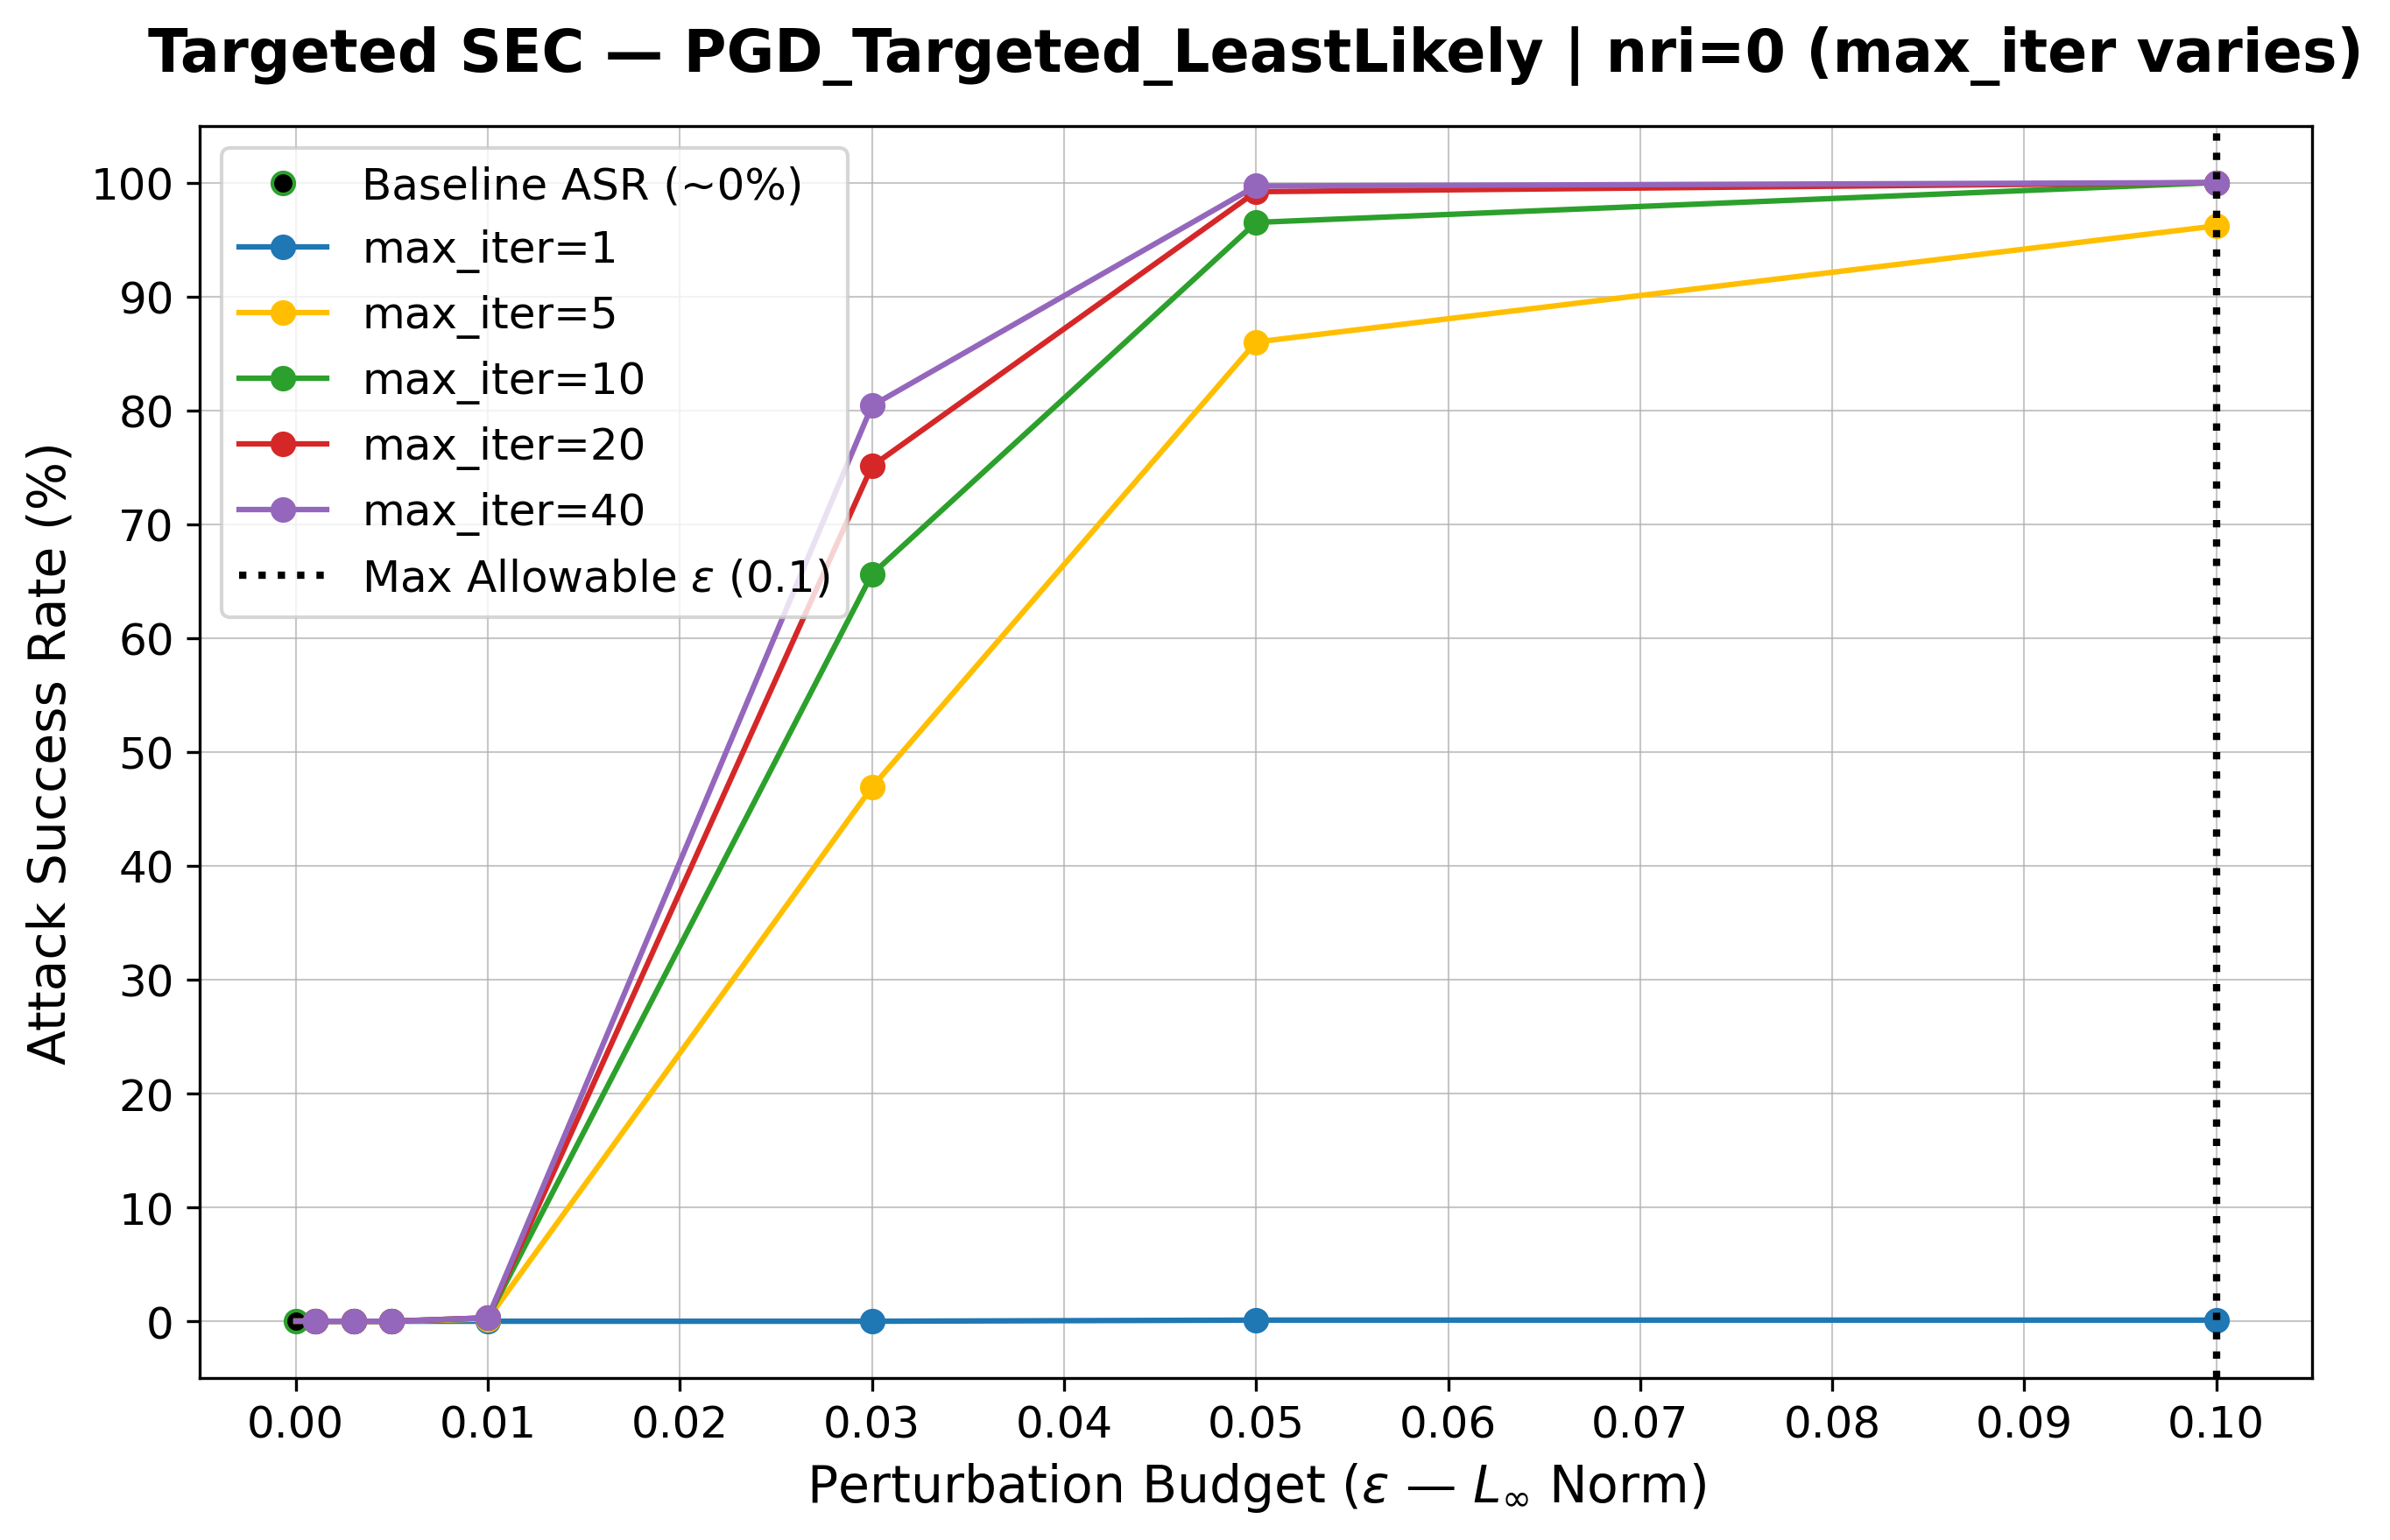
\includegraphics[width=0.5\linewidth]{PGD_Error_specific/LL/PGD_Targeted_LeastLikely_nri0_comparative_maxiter_SEC.png}
    \caption{PGD Least Likely SEC con nri = 0}
    \label{fig:PGD_LL_SEC_nri0}
\end{figure}

% -- SOTTO GRAFICI PER NRI = 0
\begin{figure}[H]
    \centering
    % Sotto-figura 1
    \begin{subfigure}[b]{0.45\textwidth}
        \centering
        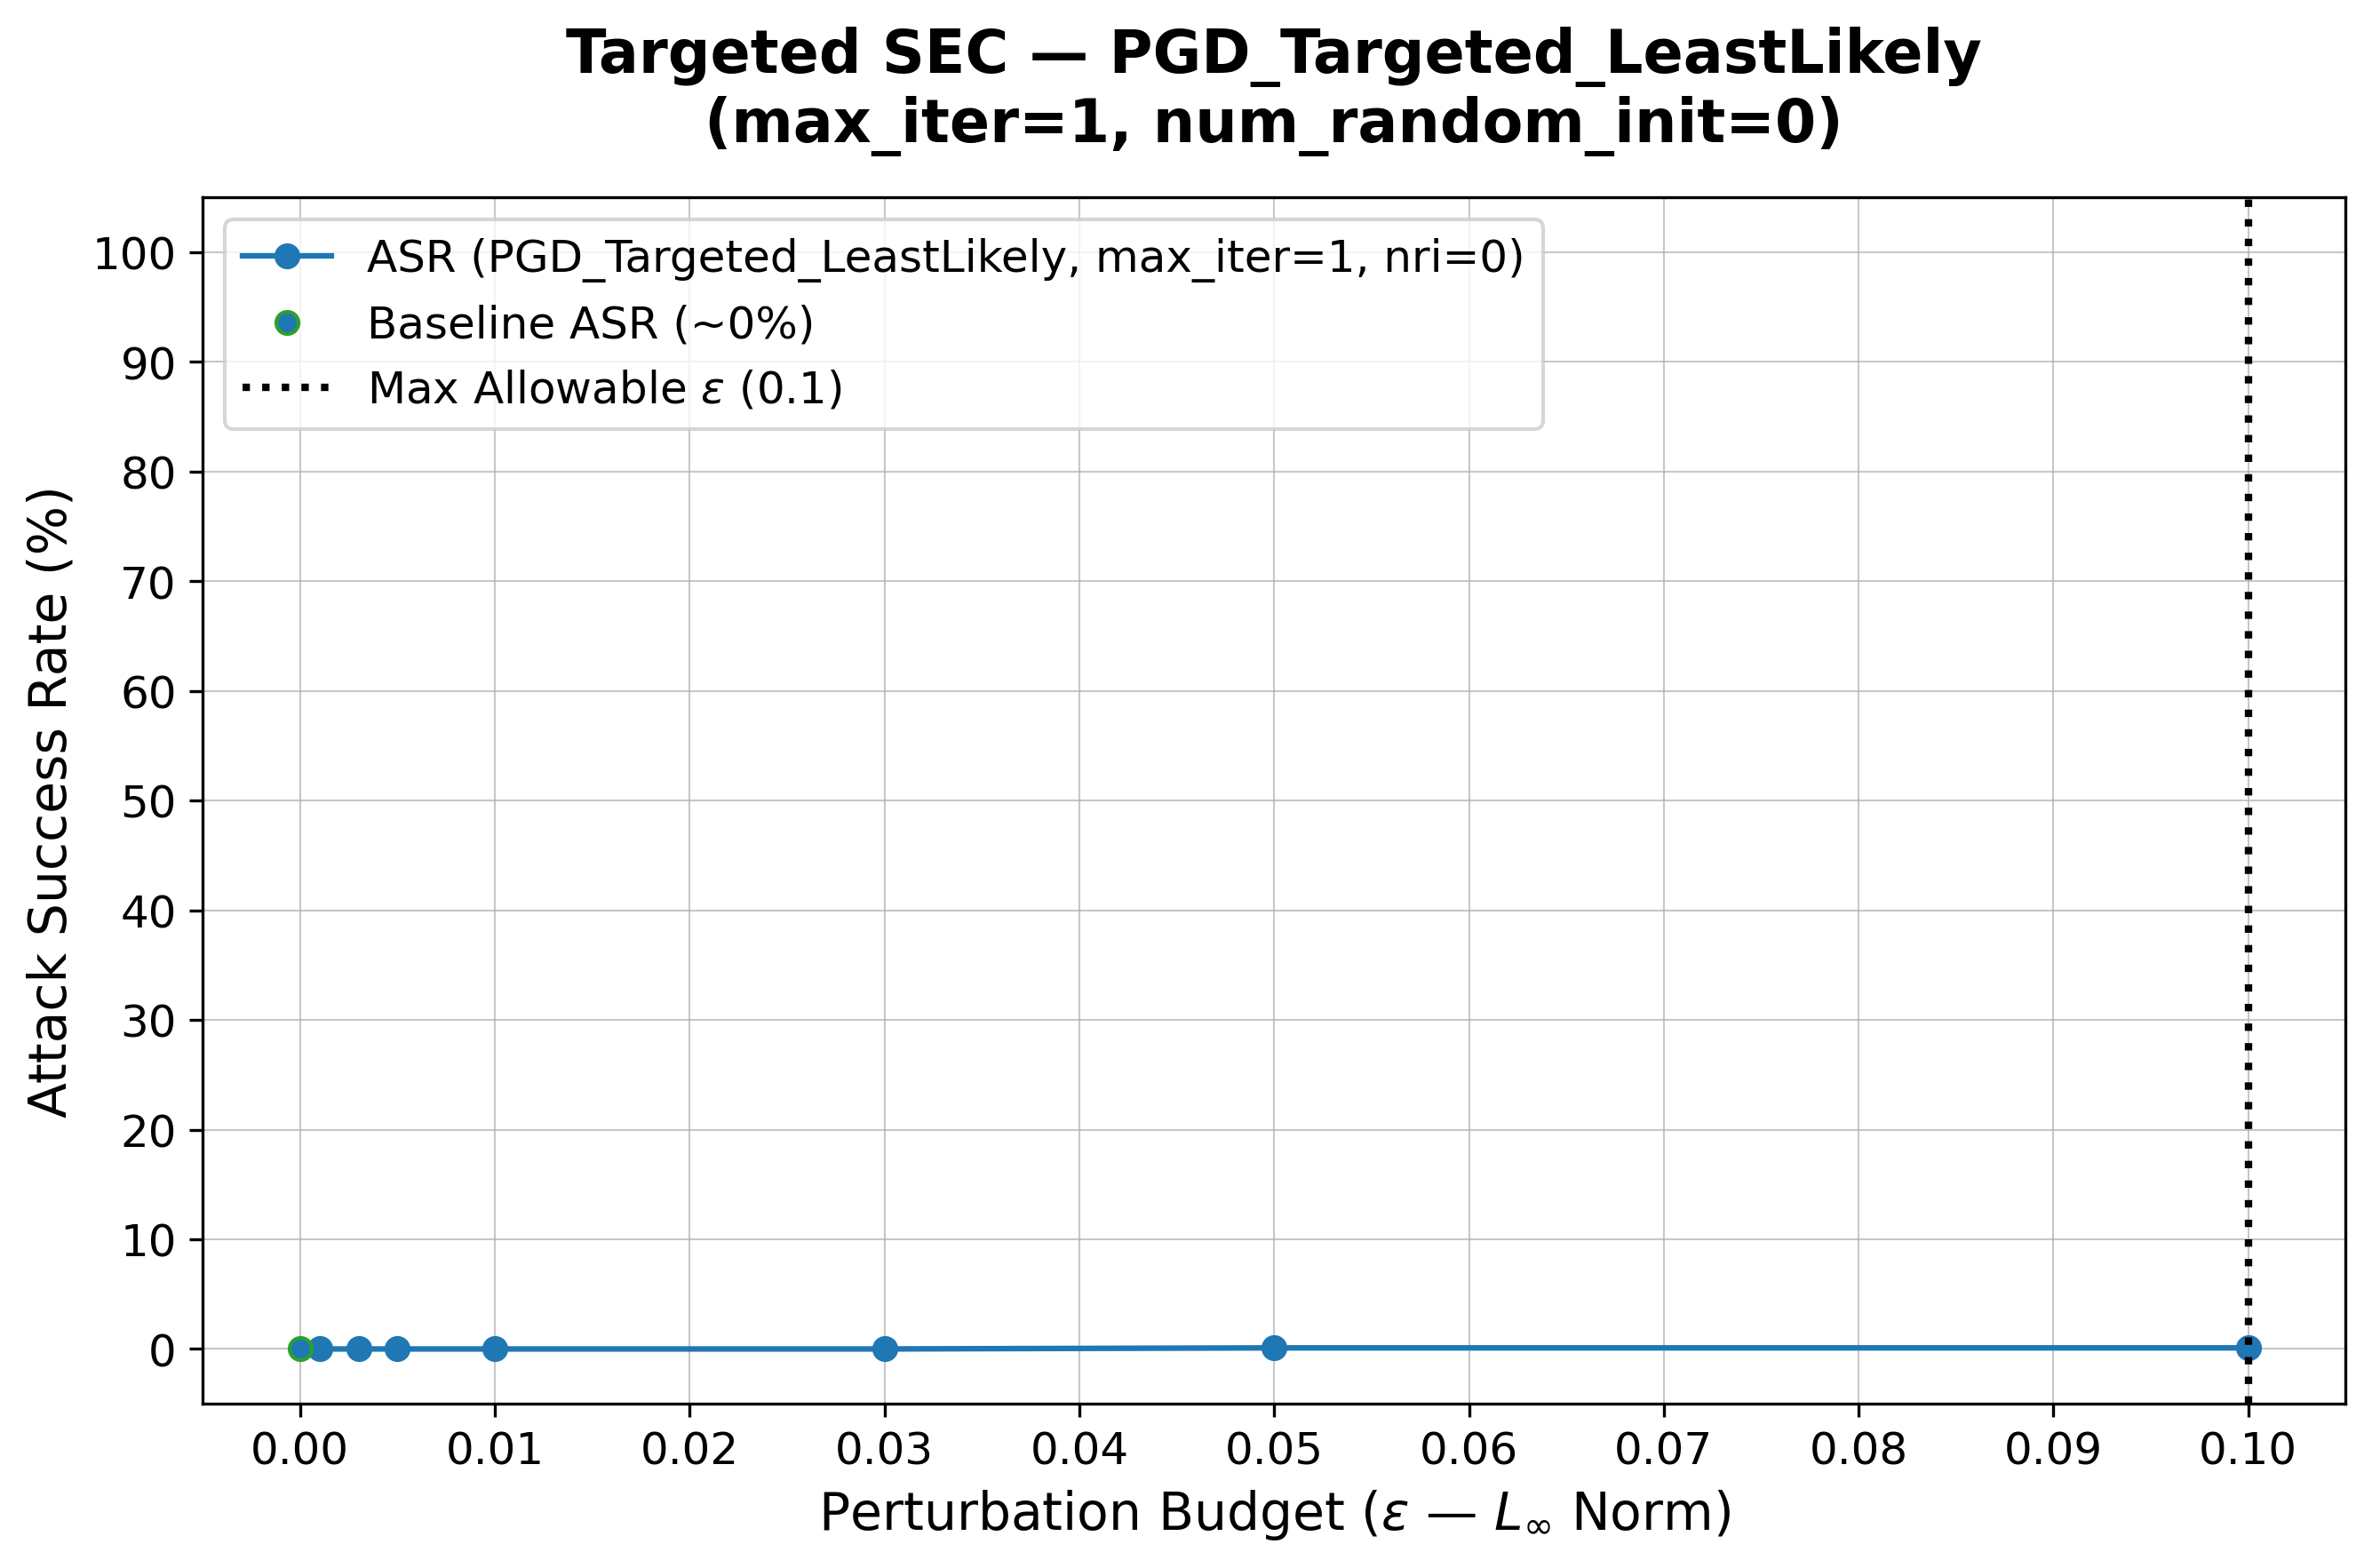
\includegraphics[width=\textwidth]{PGD_Error_specific/LL/PGD_Targeted_LeastLikely_nri0_iter1_SEC.png}
        \caption{\texttt{max_iter} = 1}
        \label{fig:PGD_LL_nri0_iter1}
    \end{subfigure}
    \hfill
    % Sotto-figura 2
    \begin{subfigure}[b]{0.45\textwidth}
        \centering
        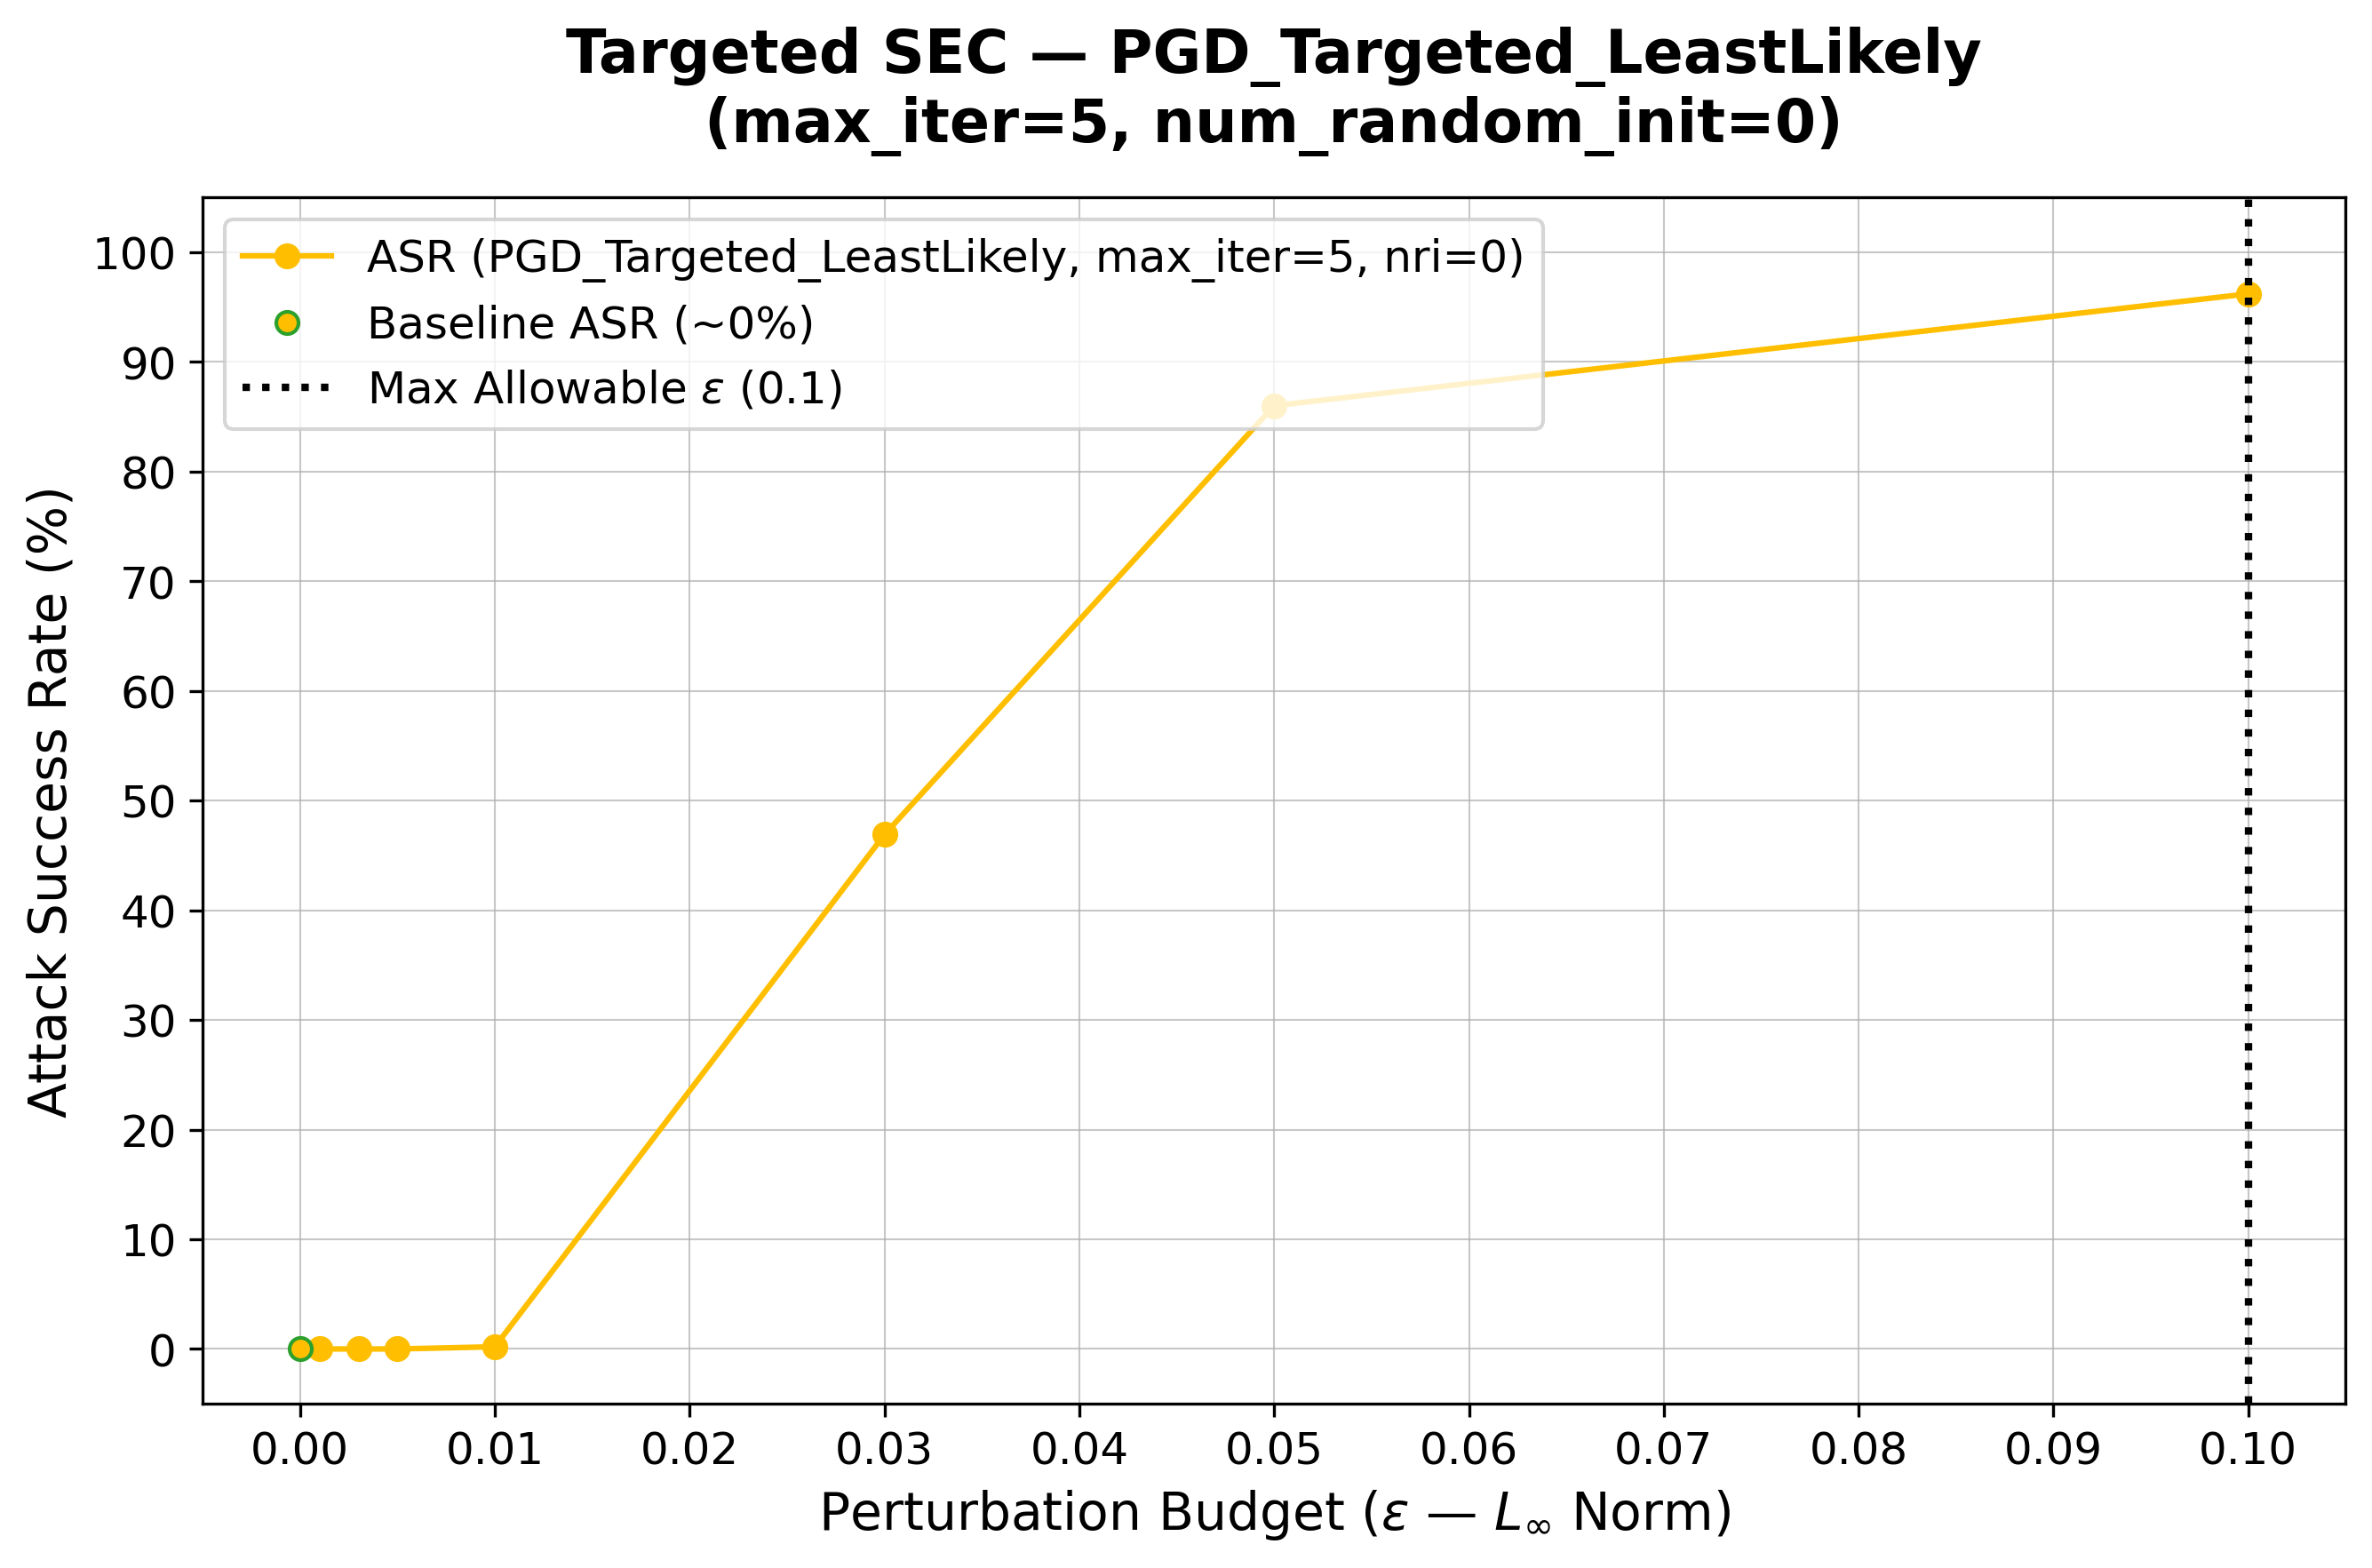
\includegraphics[width=\textwidth]{PGD_Error_specific/LL/PGD_Targeted_LeastLikely_nri0_iter5_SEC.png}
        \caption{\texttt{max_iter} = 5}
        \label{fig:PGD_LL_nri0_iter5}
    \end{subfigure}

    \vspace{1em} % Spazio verticale tra le righe di immagini   
    % Sotto-figura 3
    \begin{subfigure}[b]{0.45\textwidth}
        \centering
        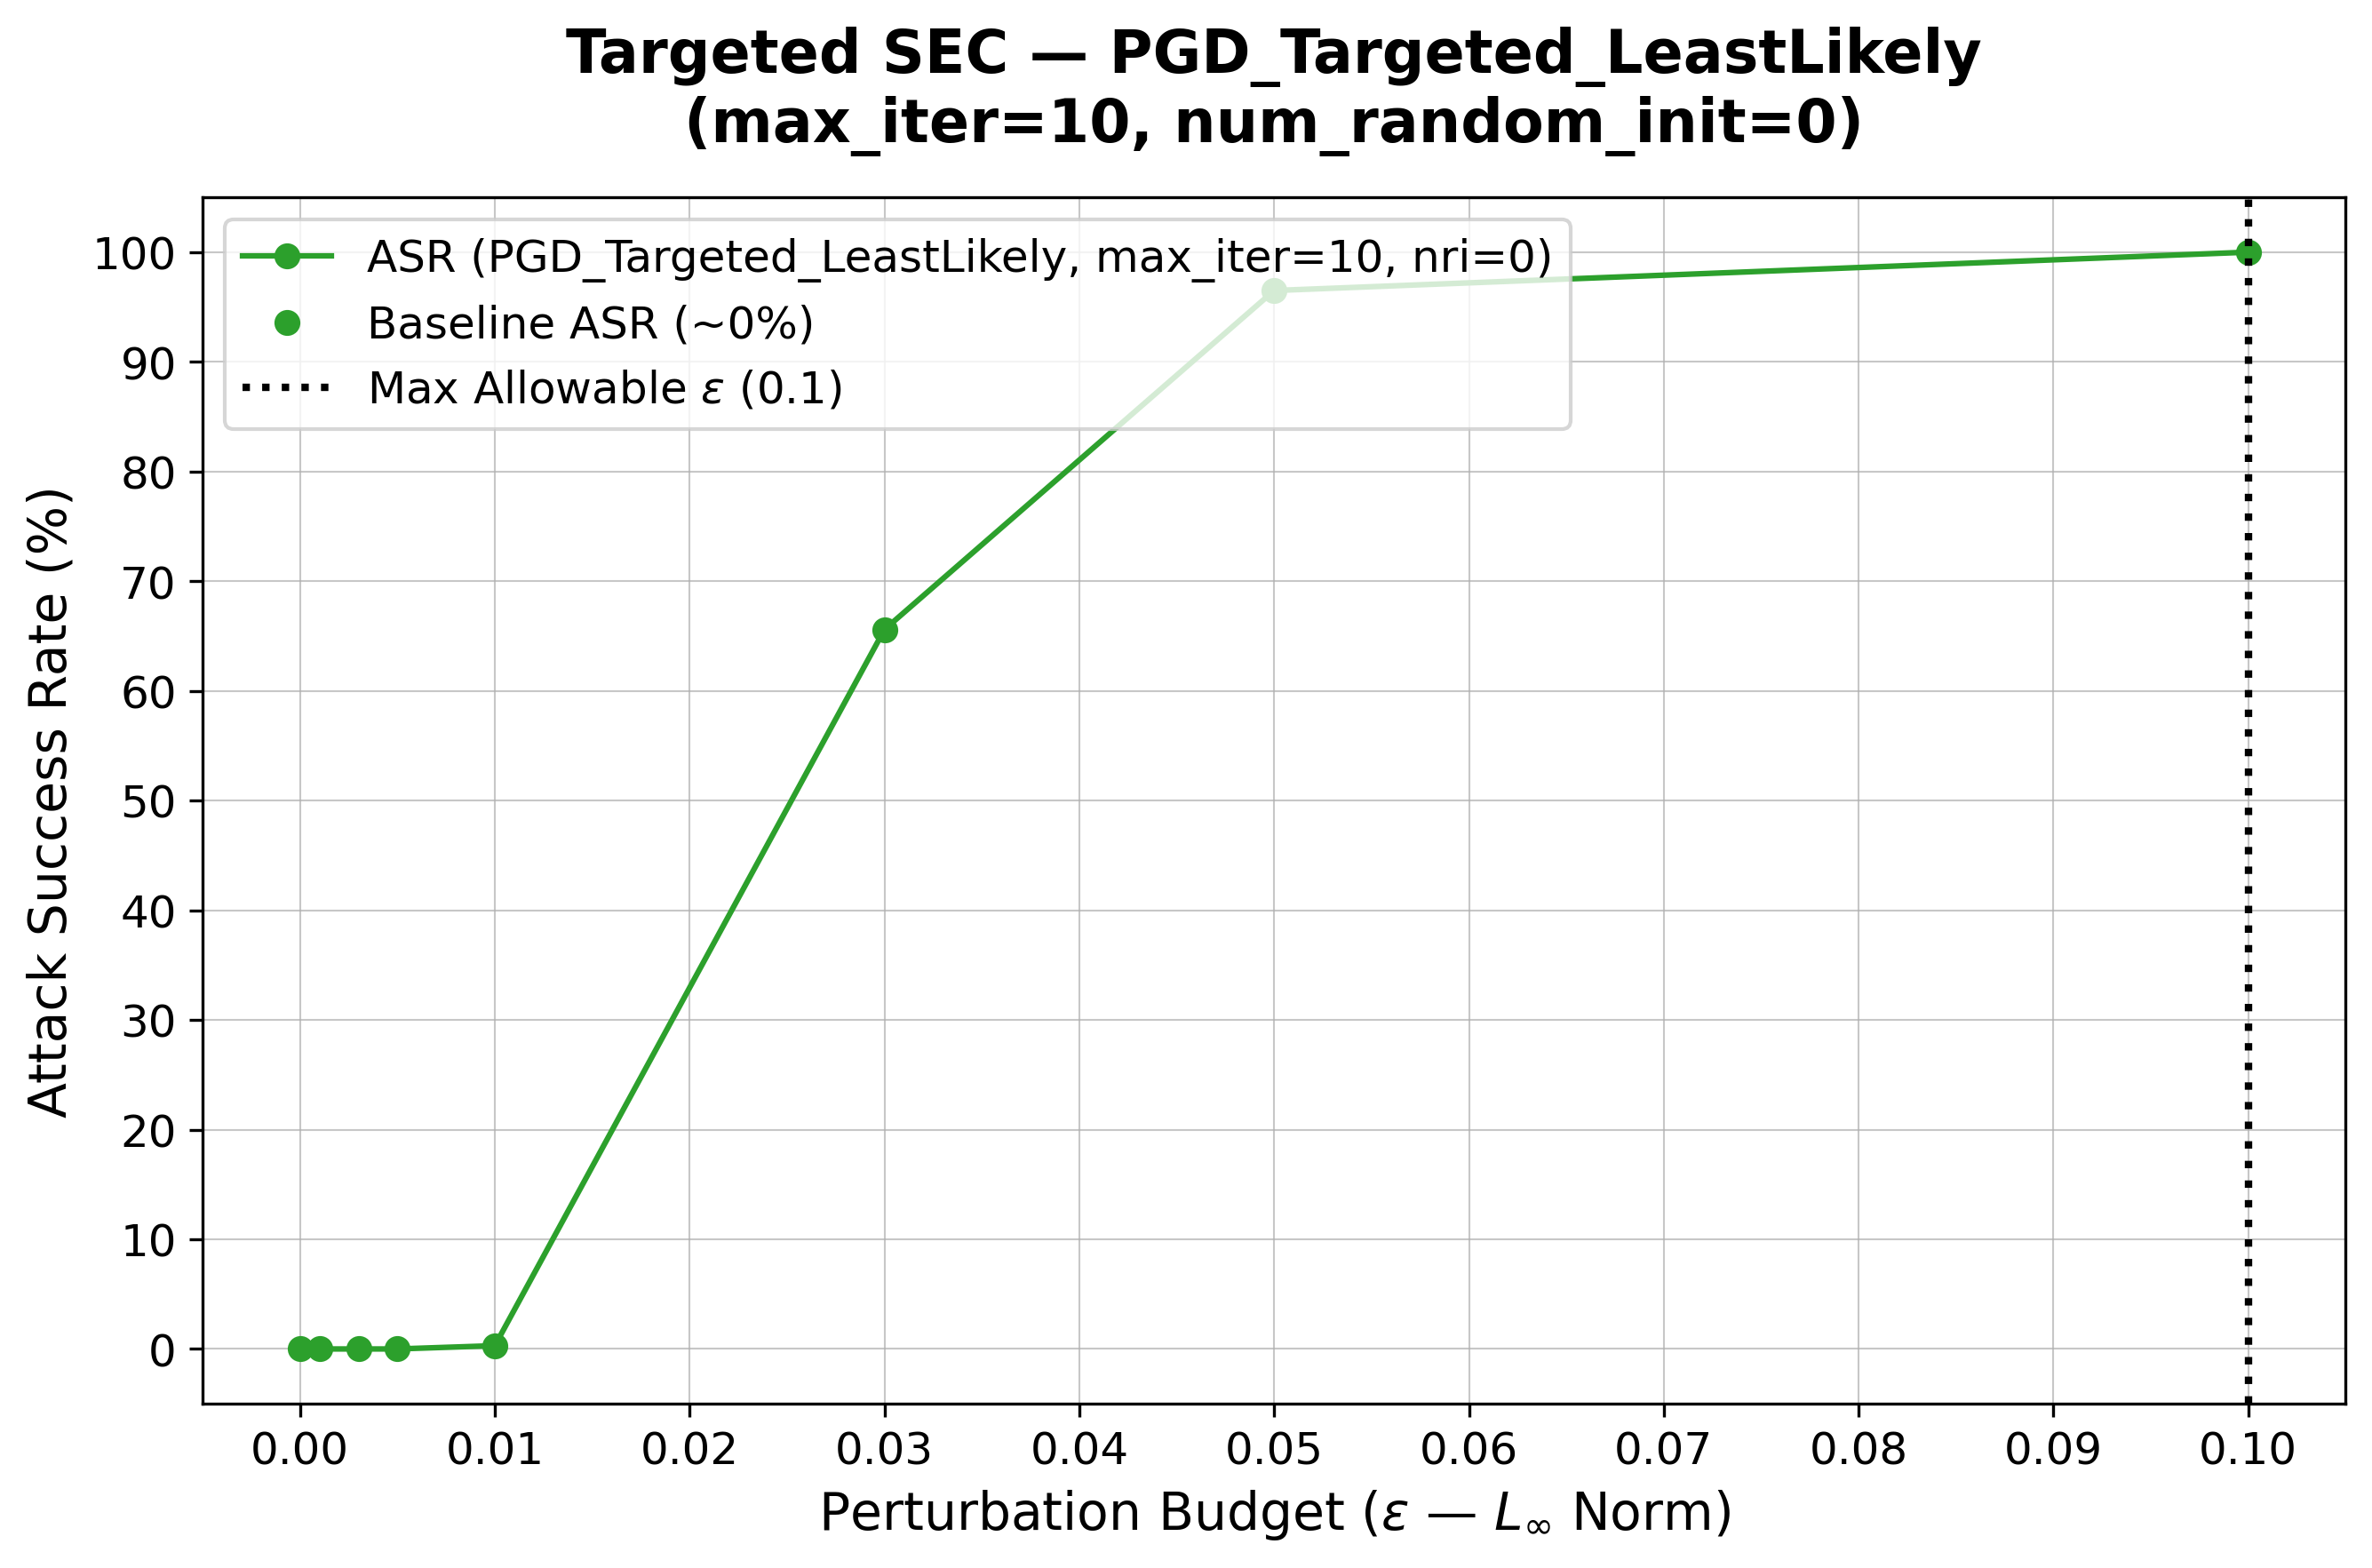
\includegraphics[width=\textwidth]{PGD_Error_specific/LL/PGD_Targeted_LeastLikely_nri0_iter10_SEC.png}
        \caption{\texttt{max_iter} = 10}
        \label{fig:PGD_LL_nri0_iter10}
    \end{subfigure}
    \hfill
    % Sotto-figura 4
    \begin{subfigure}[b]{0.45\textwidth}
        \centering
        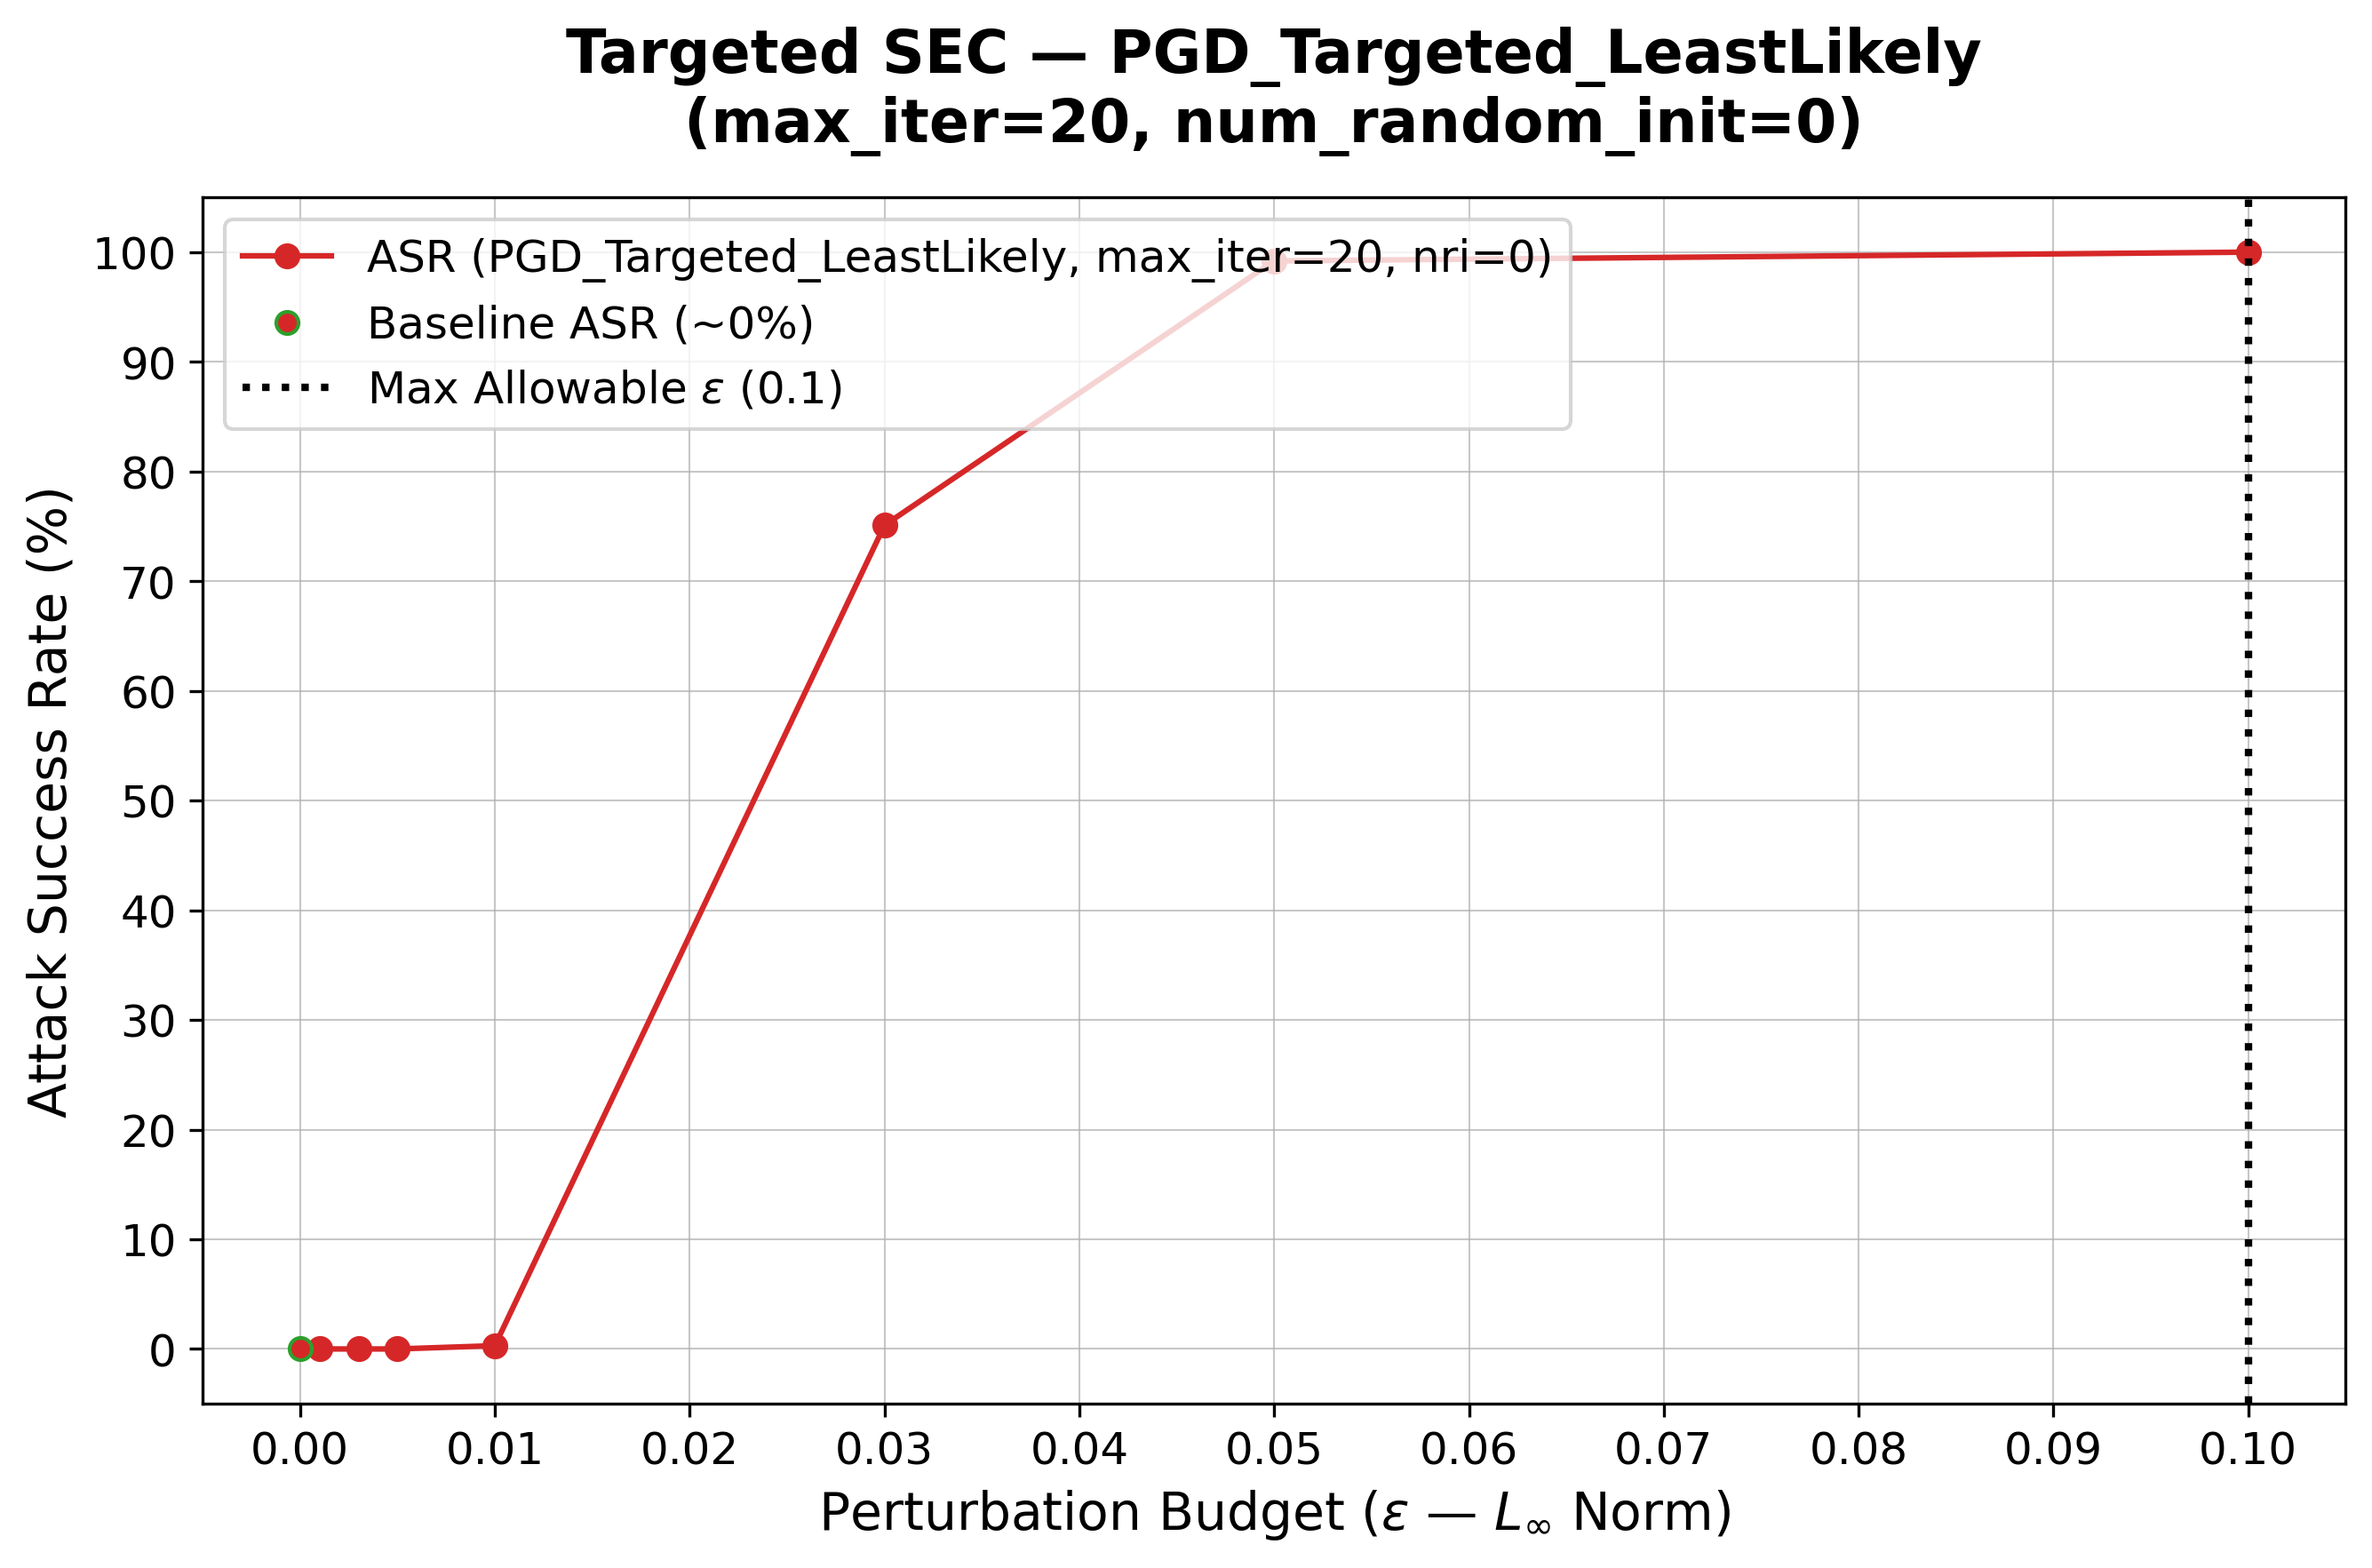
\includegraphics[width=\textwidth]{PGD_Error_specific/LL/PGD_Targeted_LeastLikely_nri0_iter20_SEC.png}
        \caption{\texttt{max_iter} = 20}
        \label{fig:PGD_LL_nri0_iter20}
    \end{subfigure}
    \vspace{1em} % Spazio verticale tra le righe di immagini
    % Sotto-figura 5
    \begin{subfigure}[b]{0.45\textwidth}
        \centering
        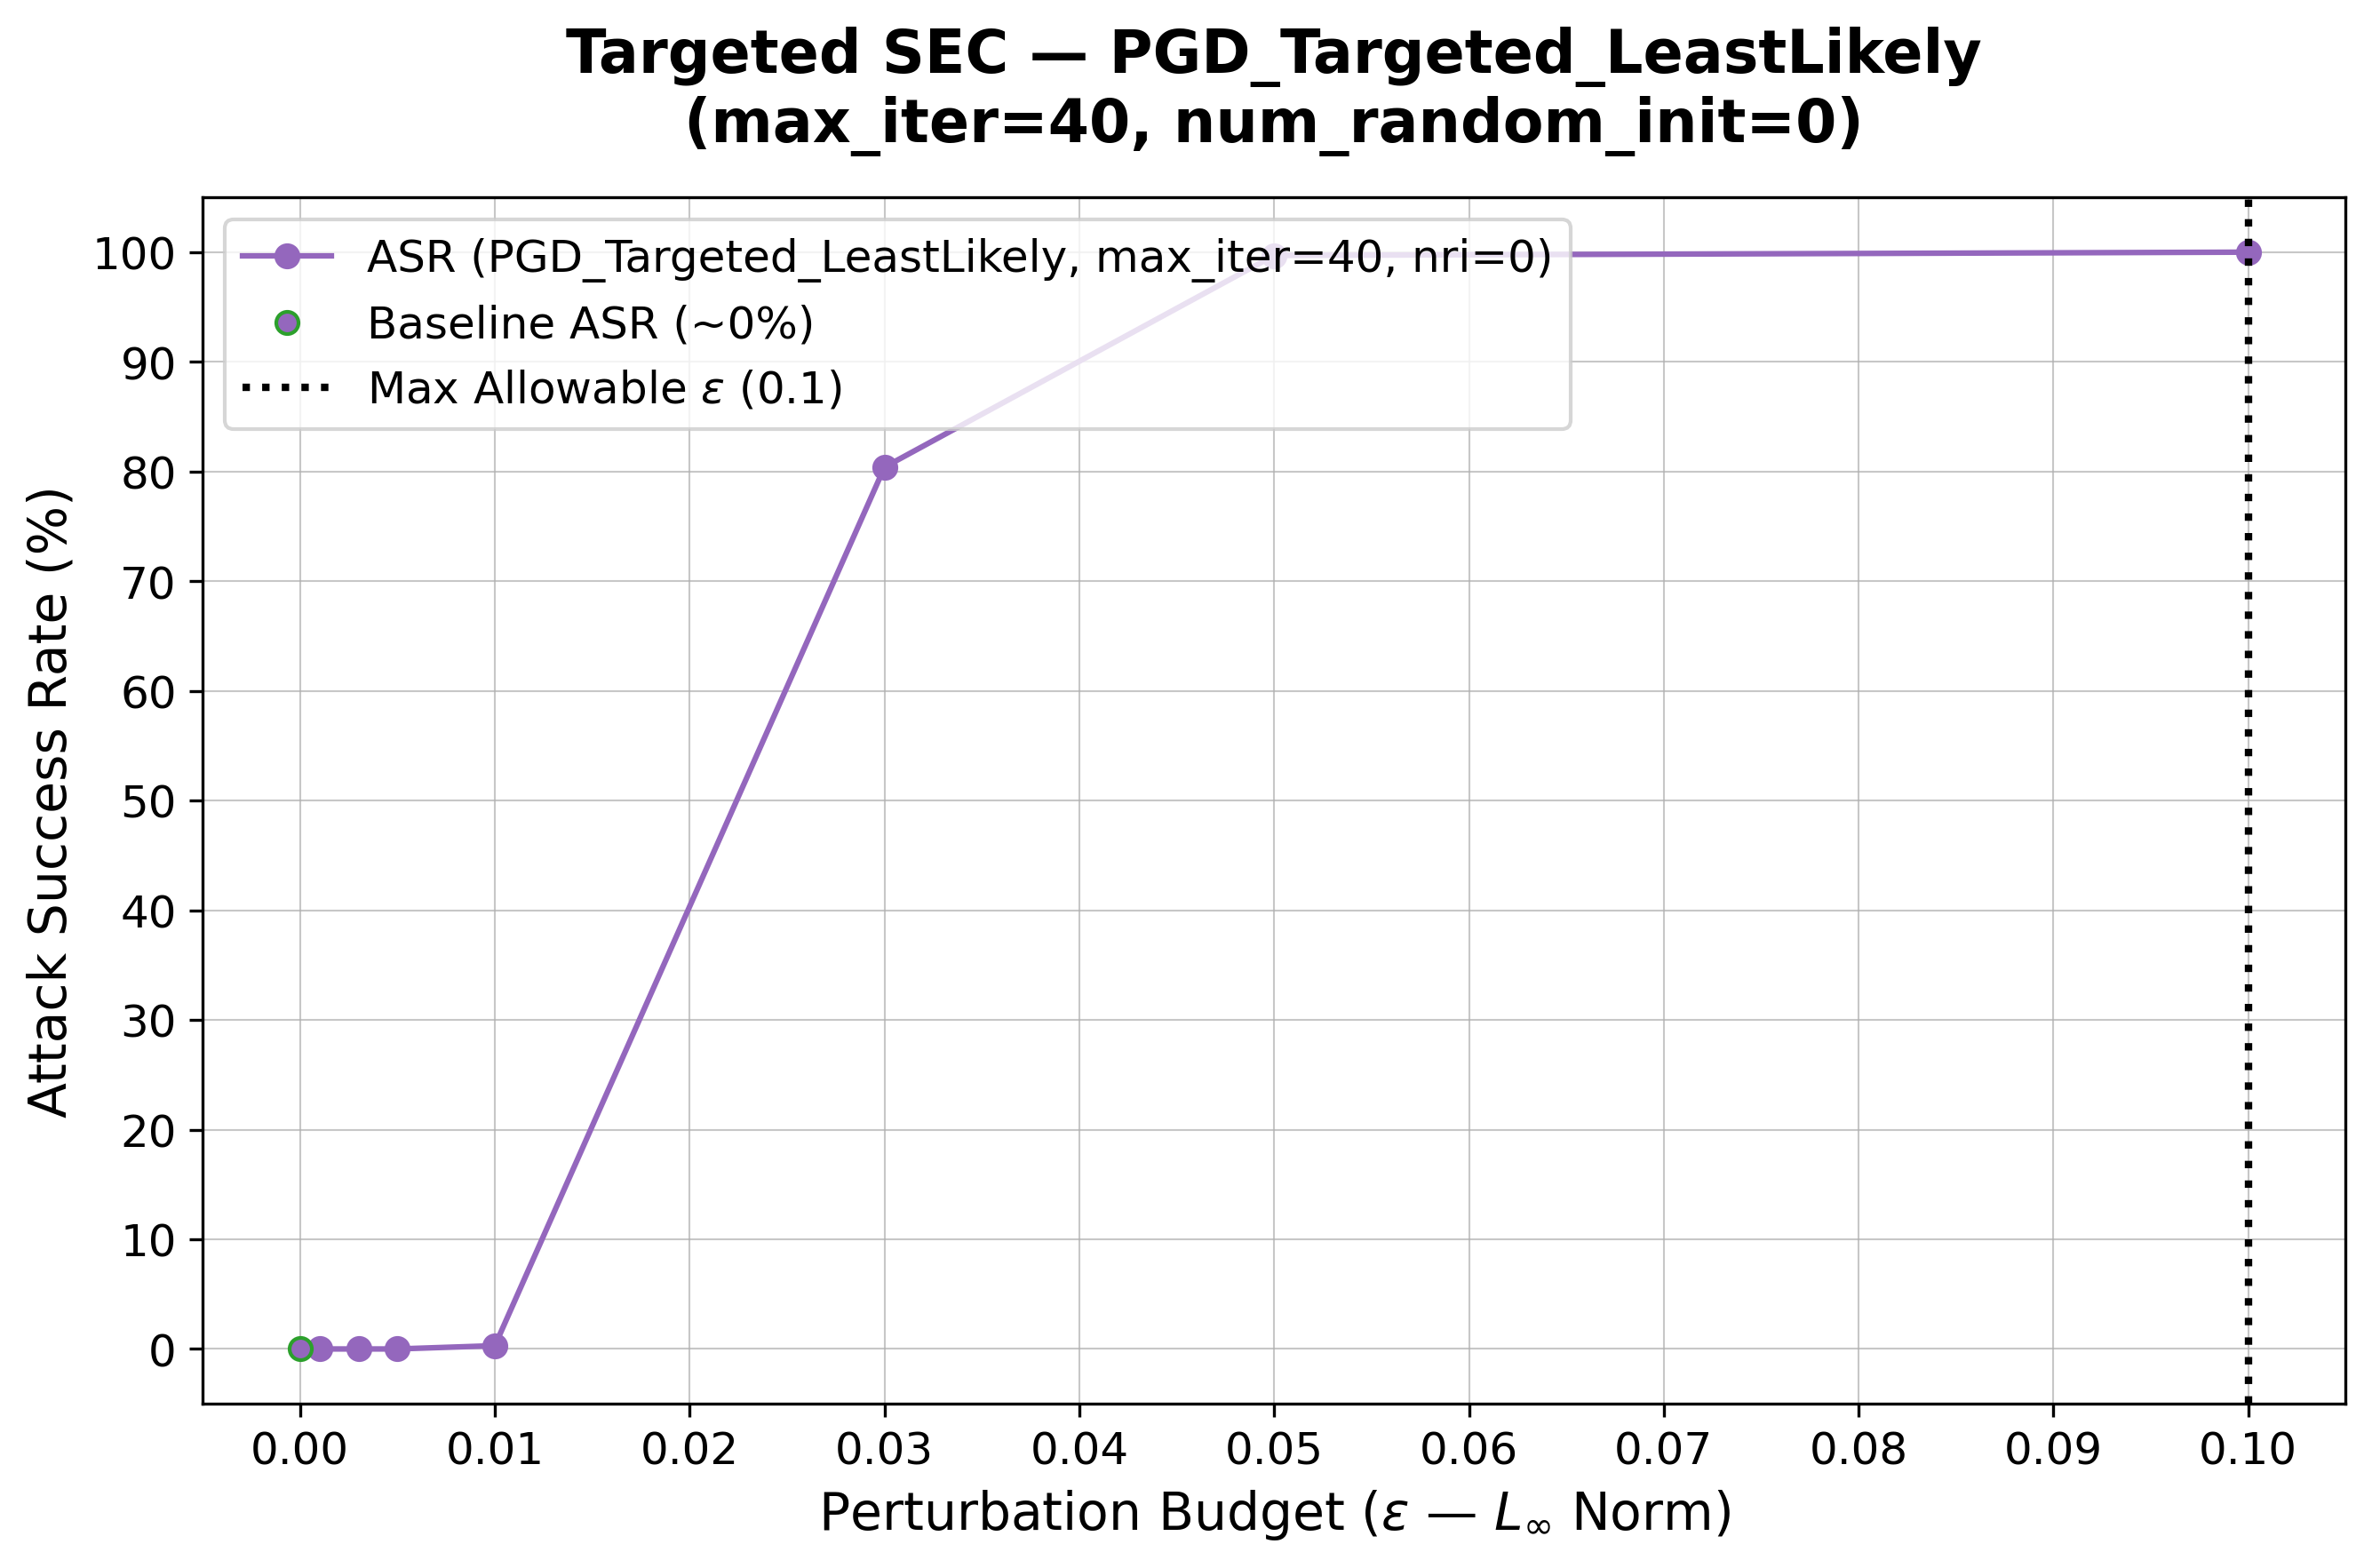
\includegraphics[width=\textwidth]{PGD_Error_specific/LL/PGD_Targeted_LeastLikely_nri0_iter40_SEC.png}
        \caption{\texttt{max_iter} = 40}
        \label{fig:PGD_LL_nri0_iter40}
    \end{subfigure}
    \caption{PGD Least Likely - Iterazioni a confronto per \texttt{nri} = 0}
    \label{fig:PGD_LL_iterations_nri0}
\end{figure}

% -- SEC NRI = 1 --
\begin{figure}[H]
    \centering
    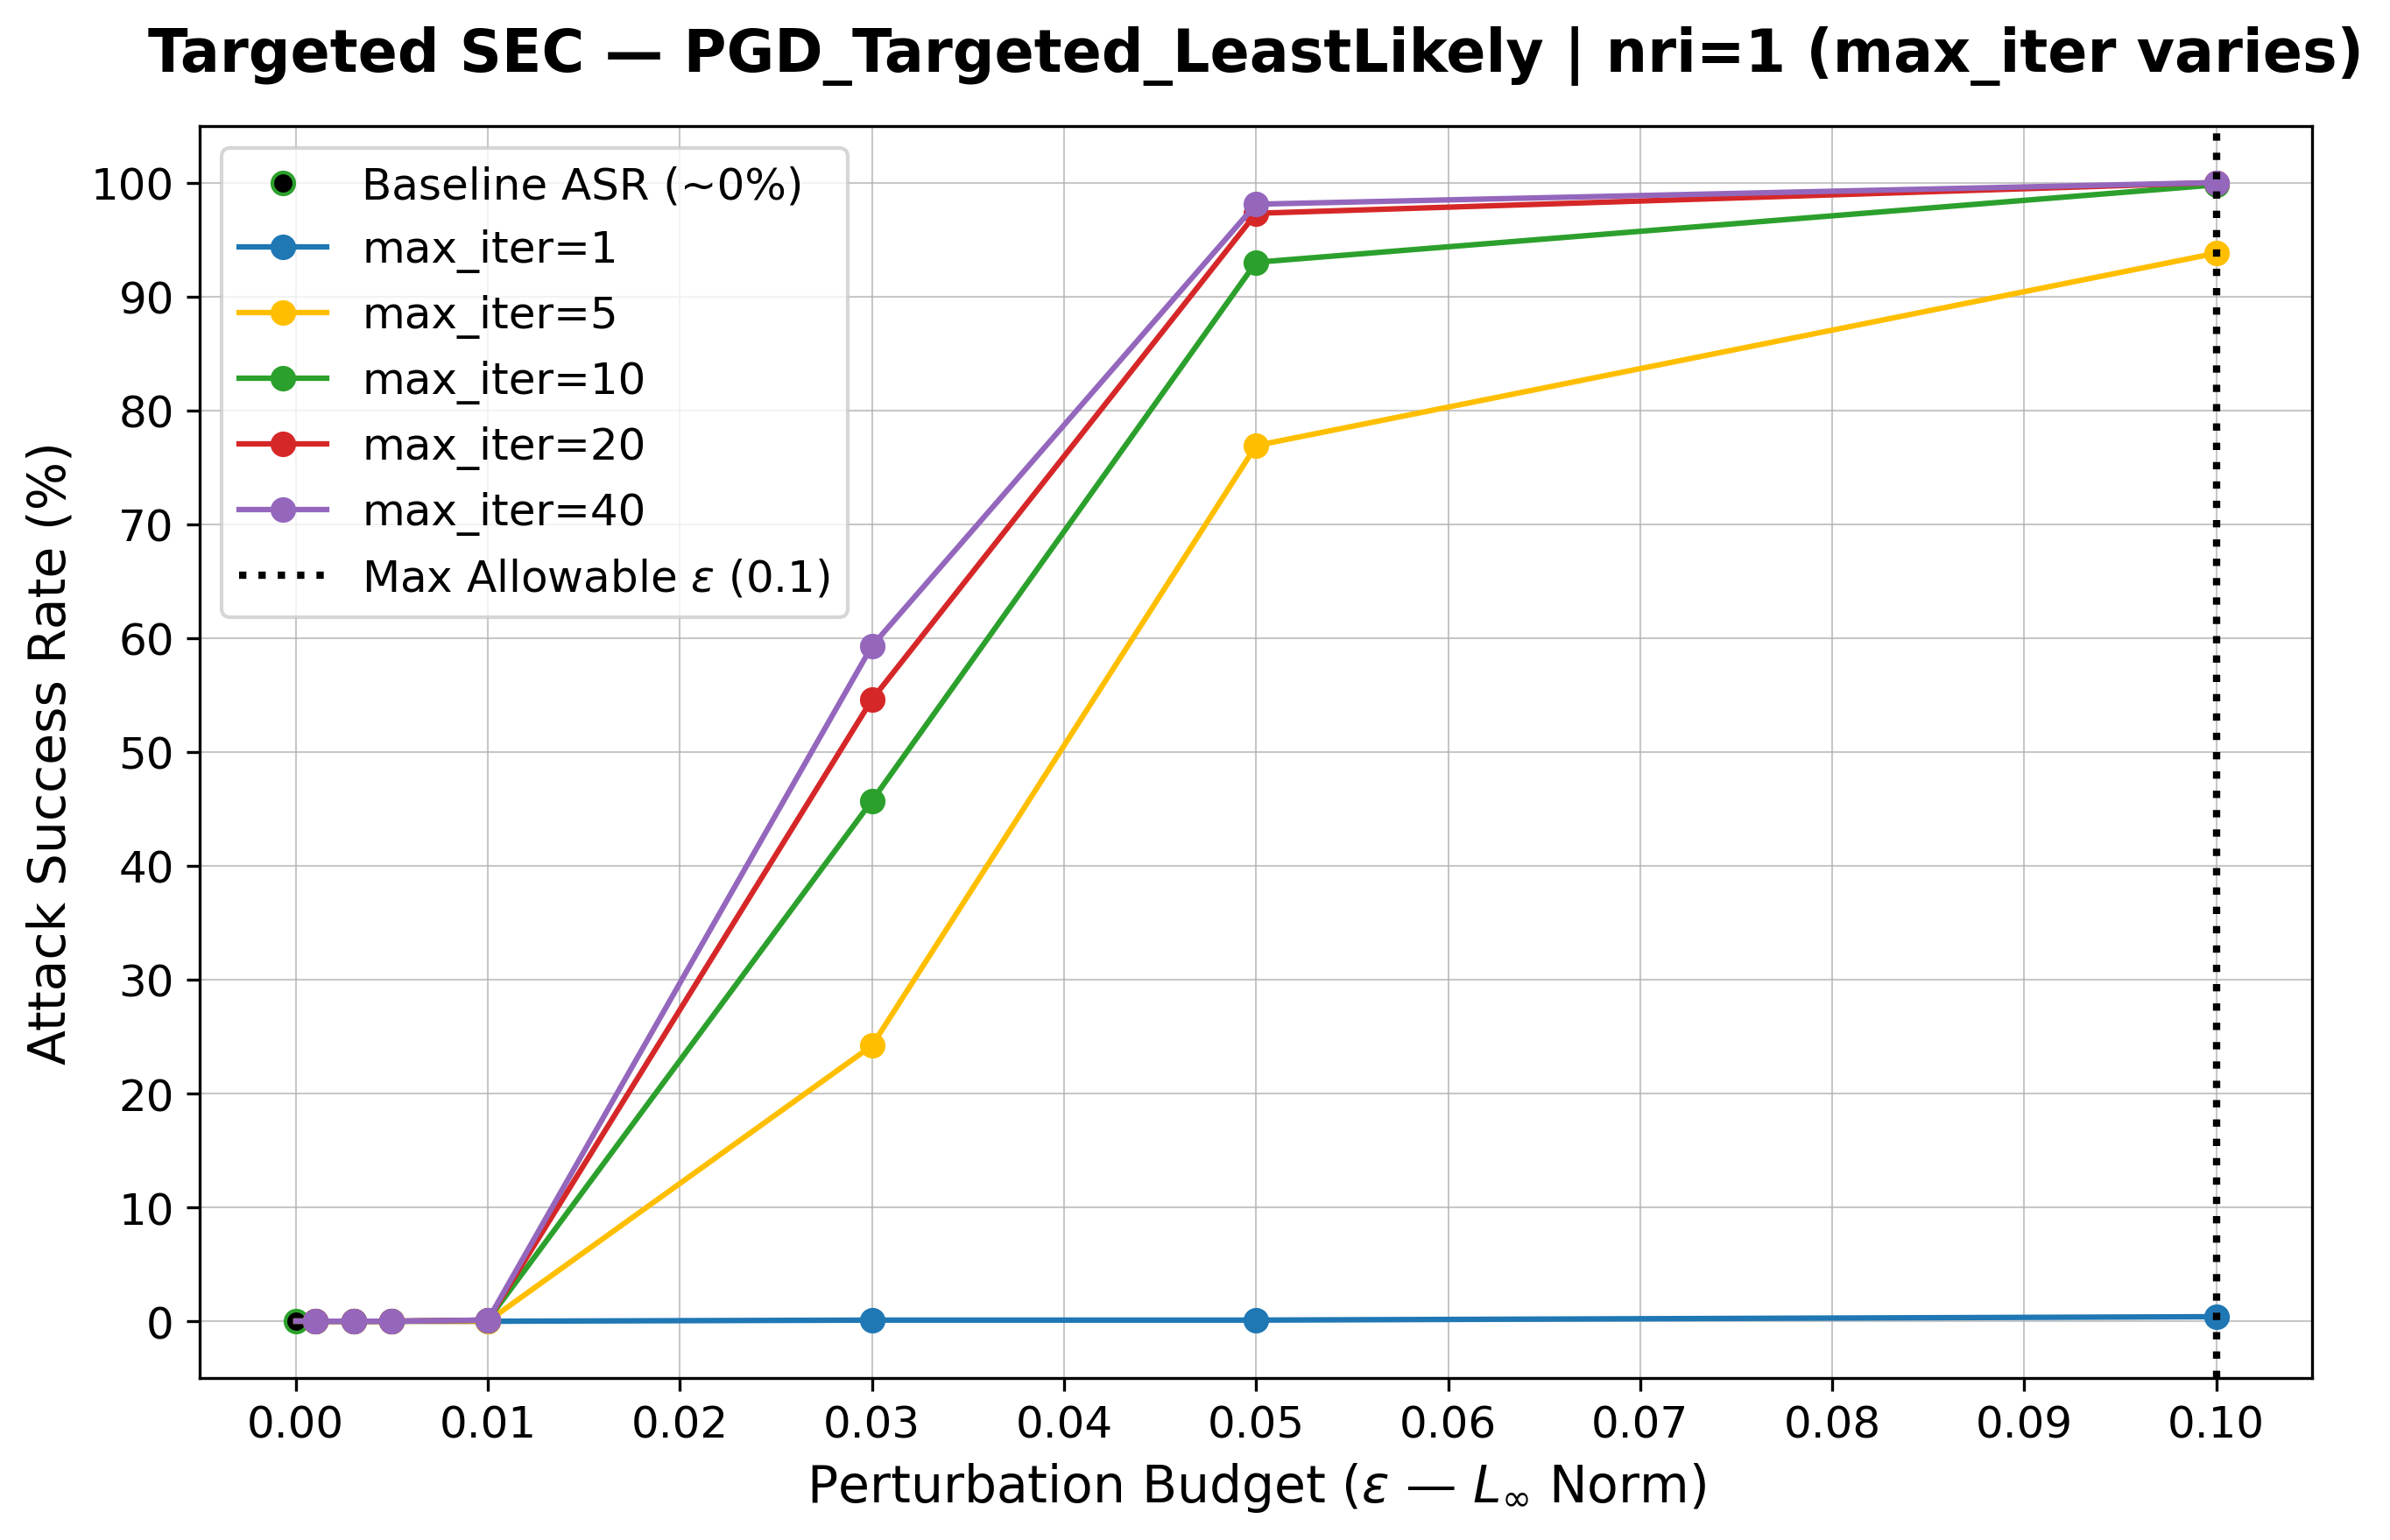
\includegraphics[width=0.5\linewidth]{PGD_Error_specific/LL/PGD_Targeted_LeastLikely_nri1_comparative_maxiter_SEC.png}
    \caption{PGD Least Likely SEC con nri = 1}
    \label{fig:PGD_LL_SEC_nri1}
\end{figure}

% -- SOTTO GRAFICI PER NRI = 1
\begin{figure}[H]
    \centering
    % Sotto-figura 1
    \begin{subfigure}[b]{0.45\textwidth}
        \centering
        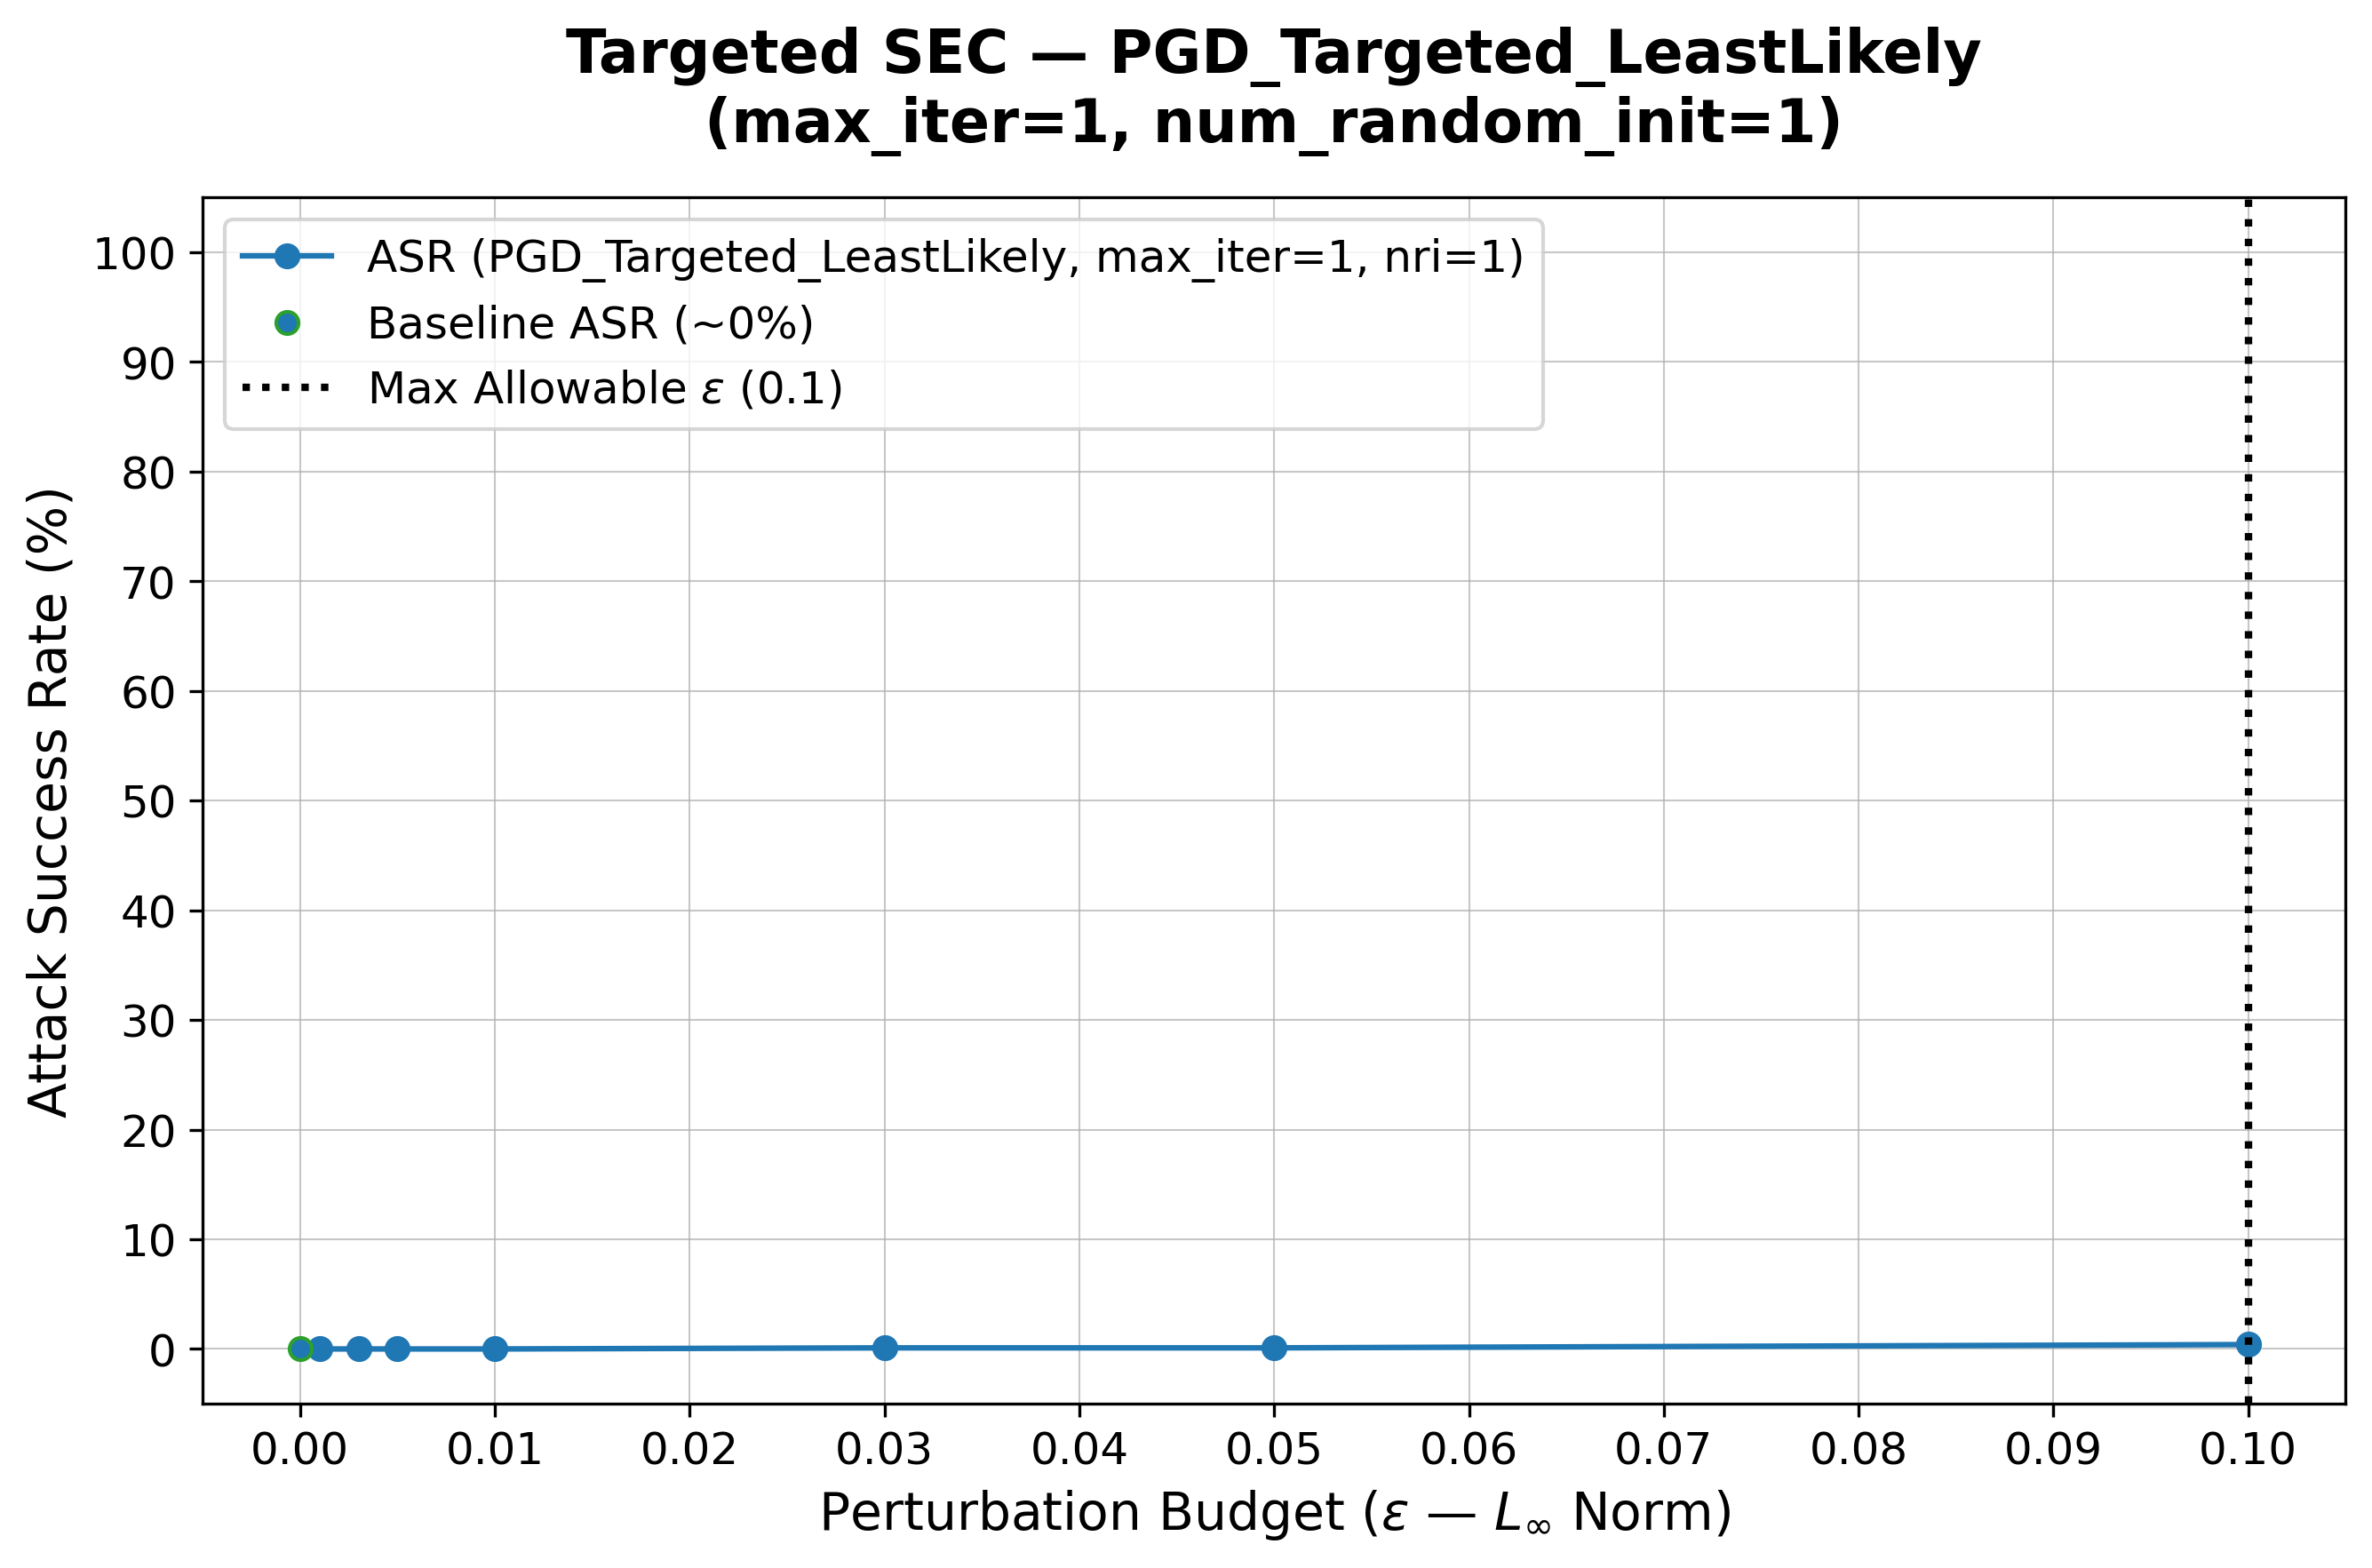
\includegraphics[width=\textwidth]{PGD_Error_specific/LL/PGD_Targeted_LeastLikely_nri1_iter1_SEC.png}
        \caption{\texttt{max_iter} = 1}
        \label{fig:PGD_LL_nri1_iter1}
    \end{subfigure}
    \hfill
    % Sotto-figura 2
    \begin{subfigure}[b]{0.45\textwidth}
        \centering
        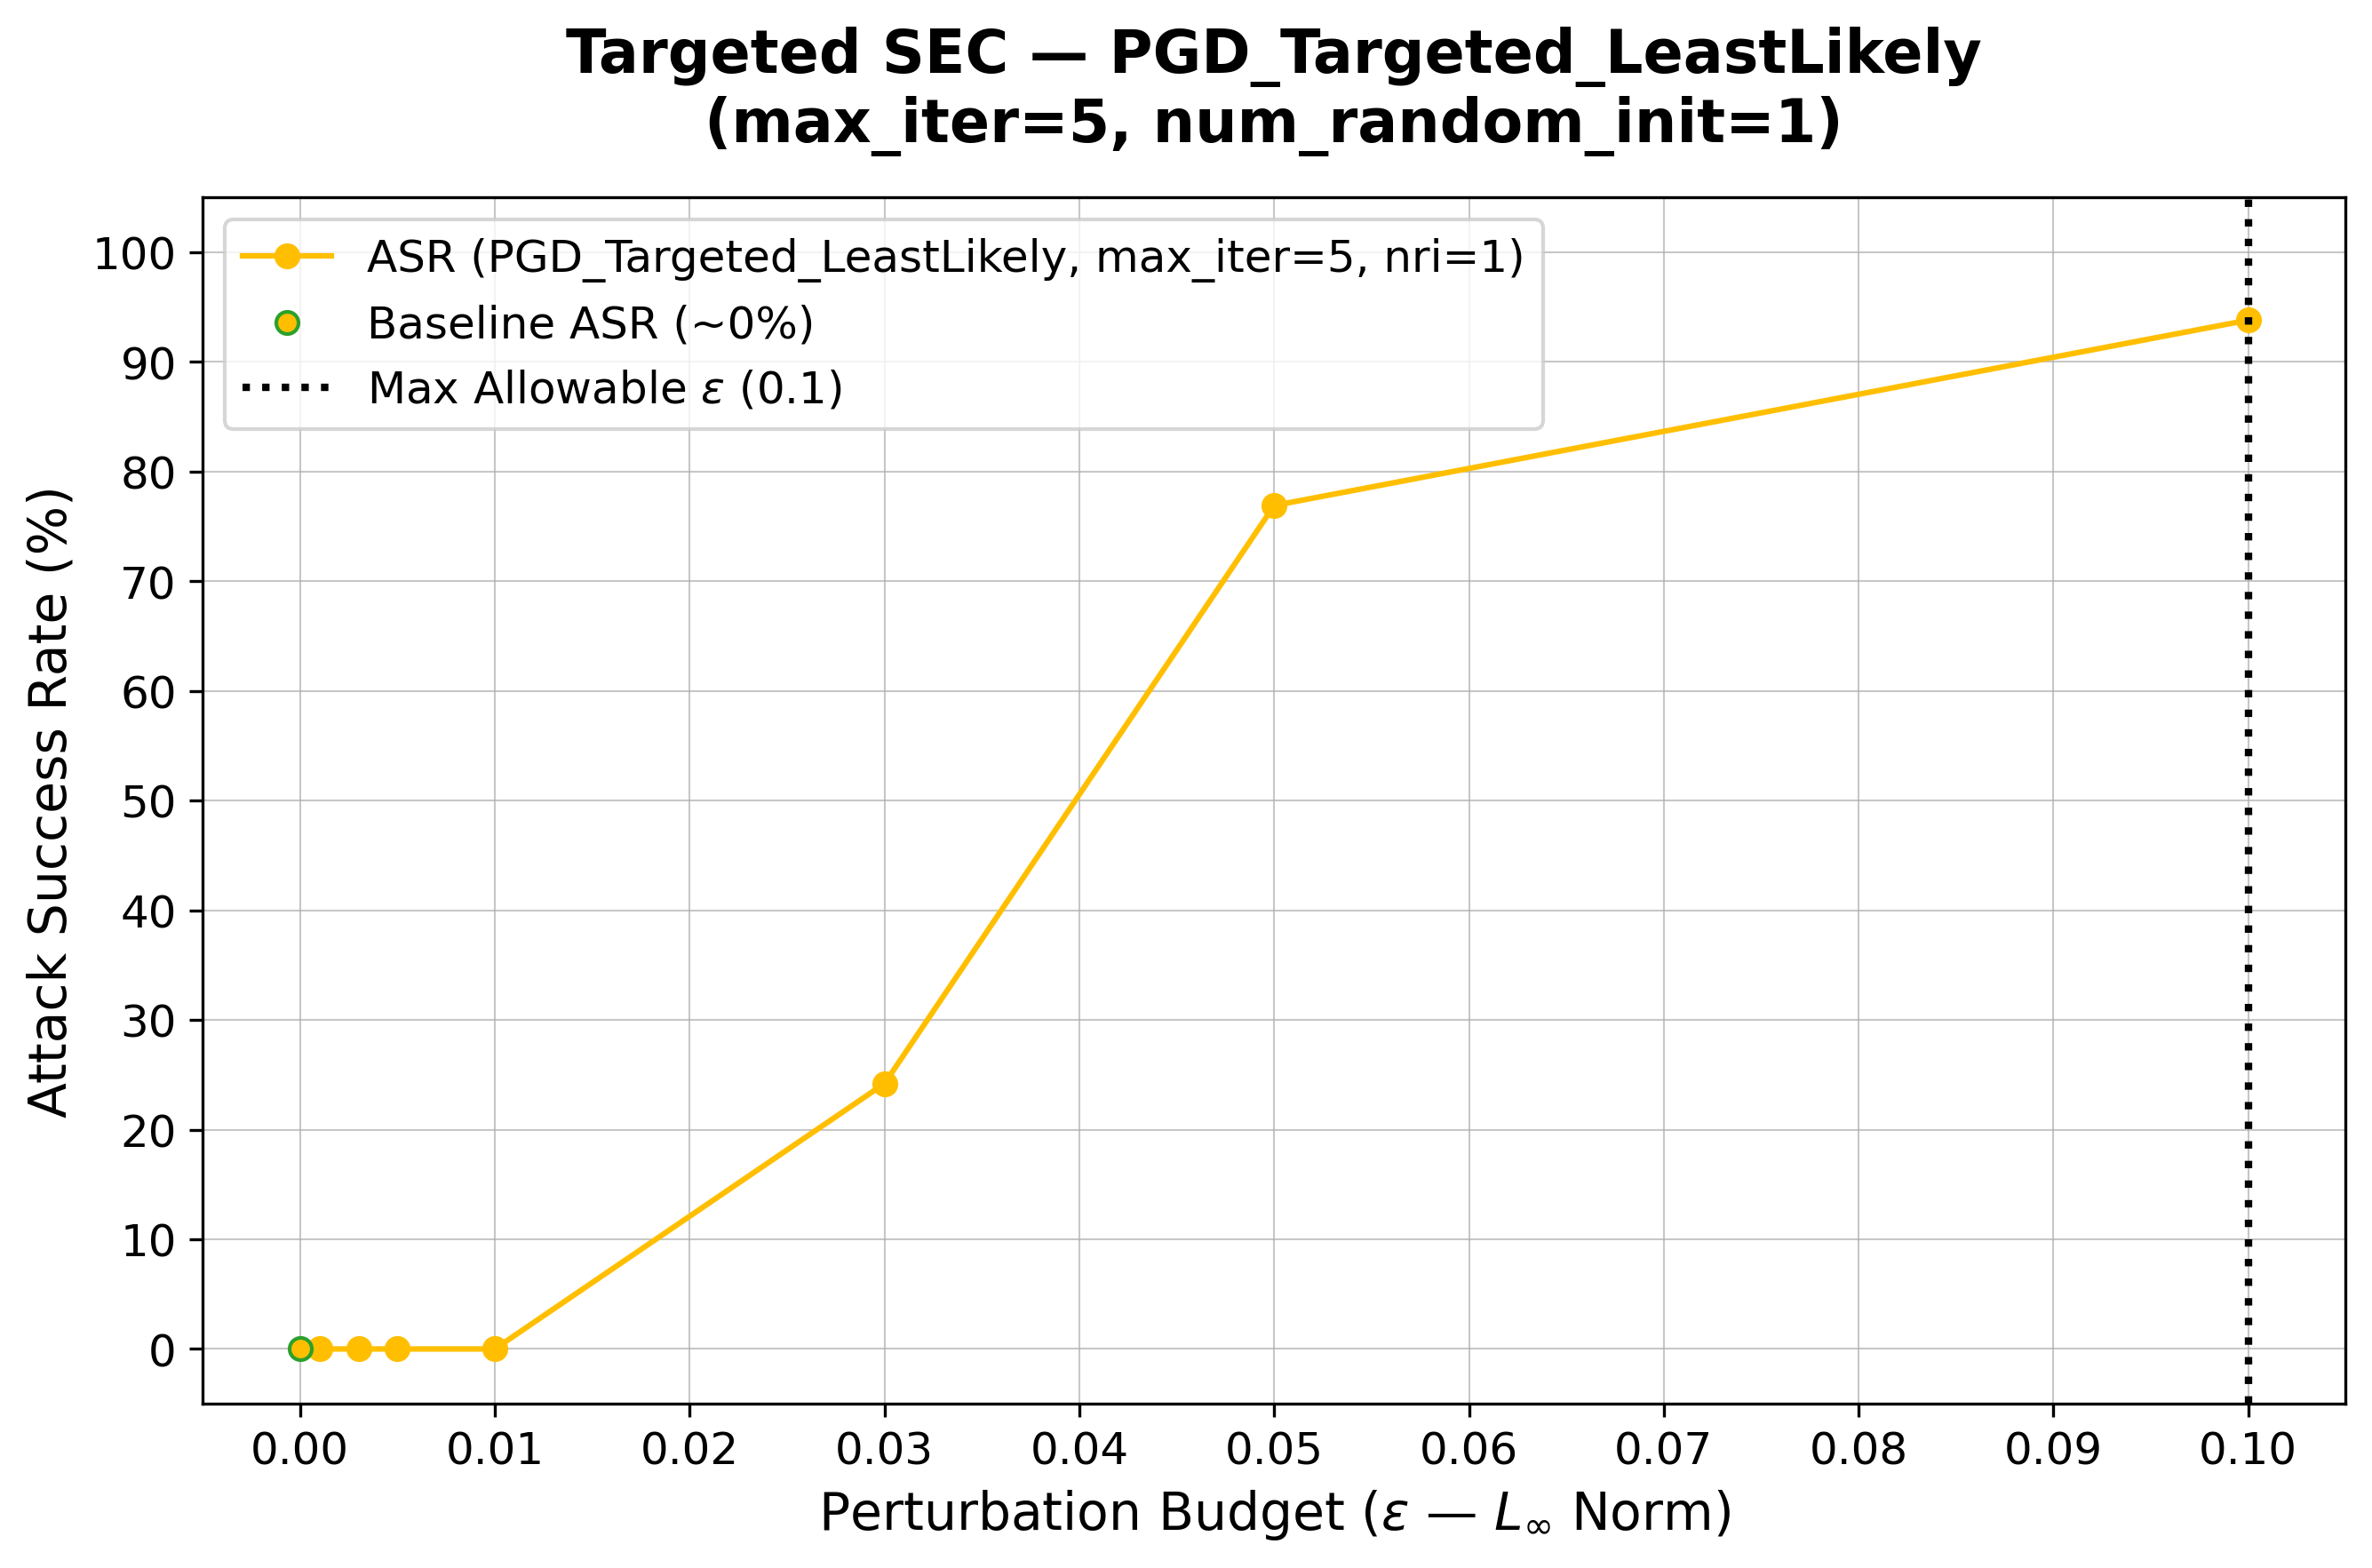
\includegraphics[width=\textwidth]{PGD_Error_specific/LL/PGD_Targeted_LeastLikely_nri1_iter5_SEC.png}
        \caption{\texttt{max_iter} = 5}
        \label{fig:PGD_LL_nri1_iter5}
    \end{subfigure} 

    \vspace{1em} % Spazio verticale tra le righe di immagini  
    % Sotto-figura 3
    \begin{subfigure}[b]{0.45\textwidth}
        \centering
        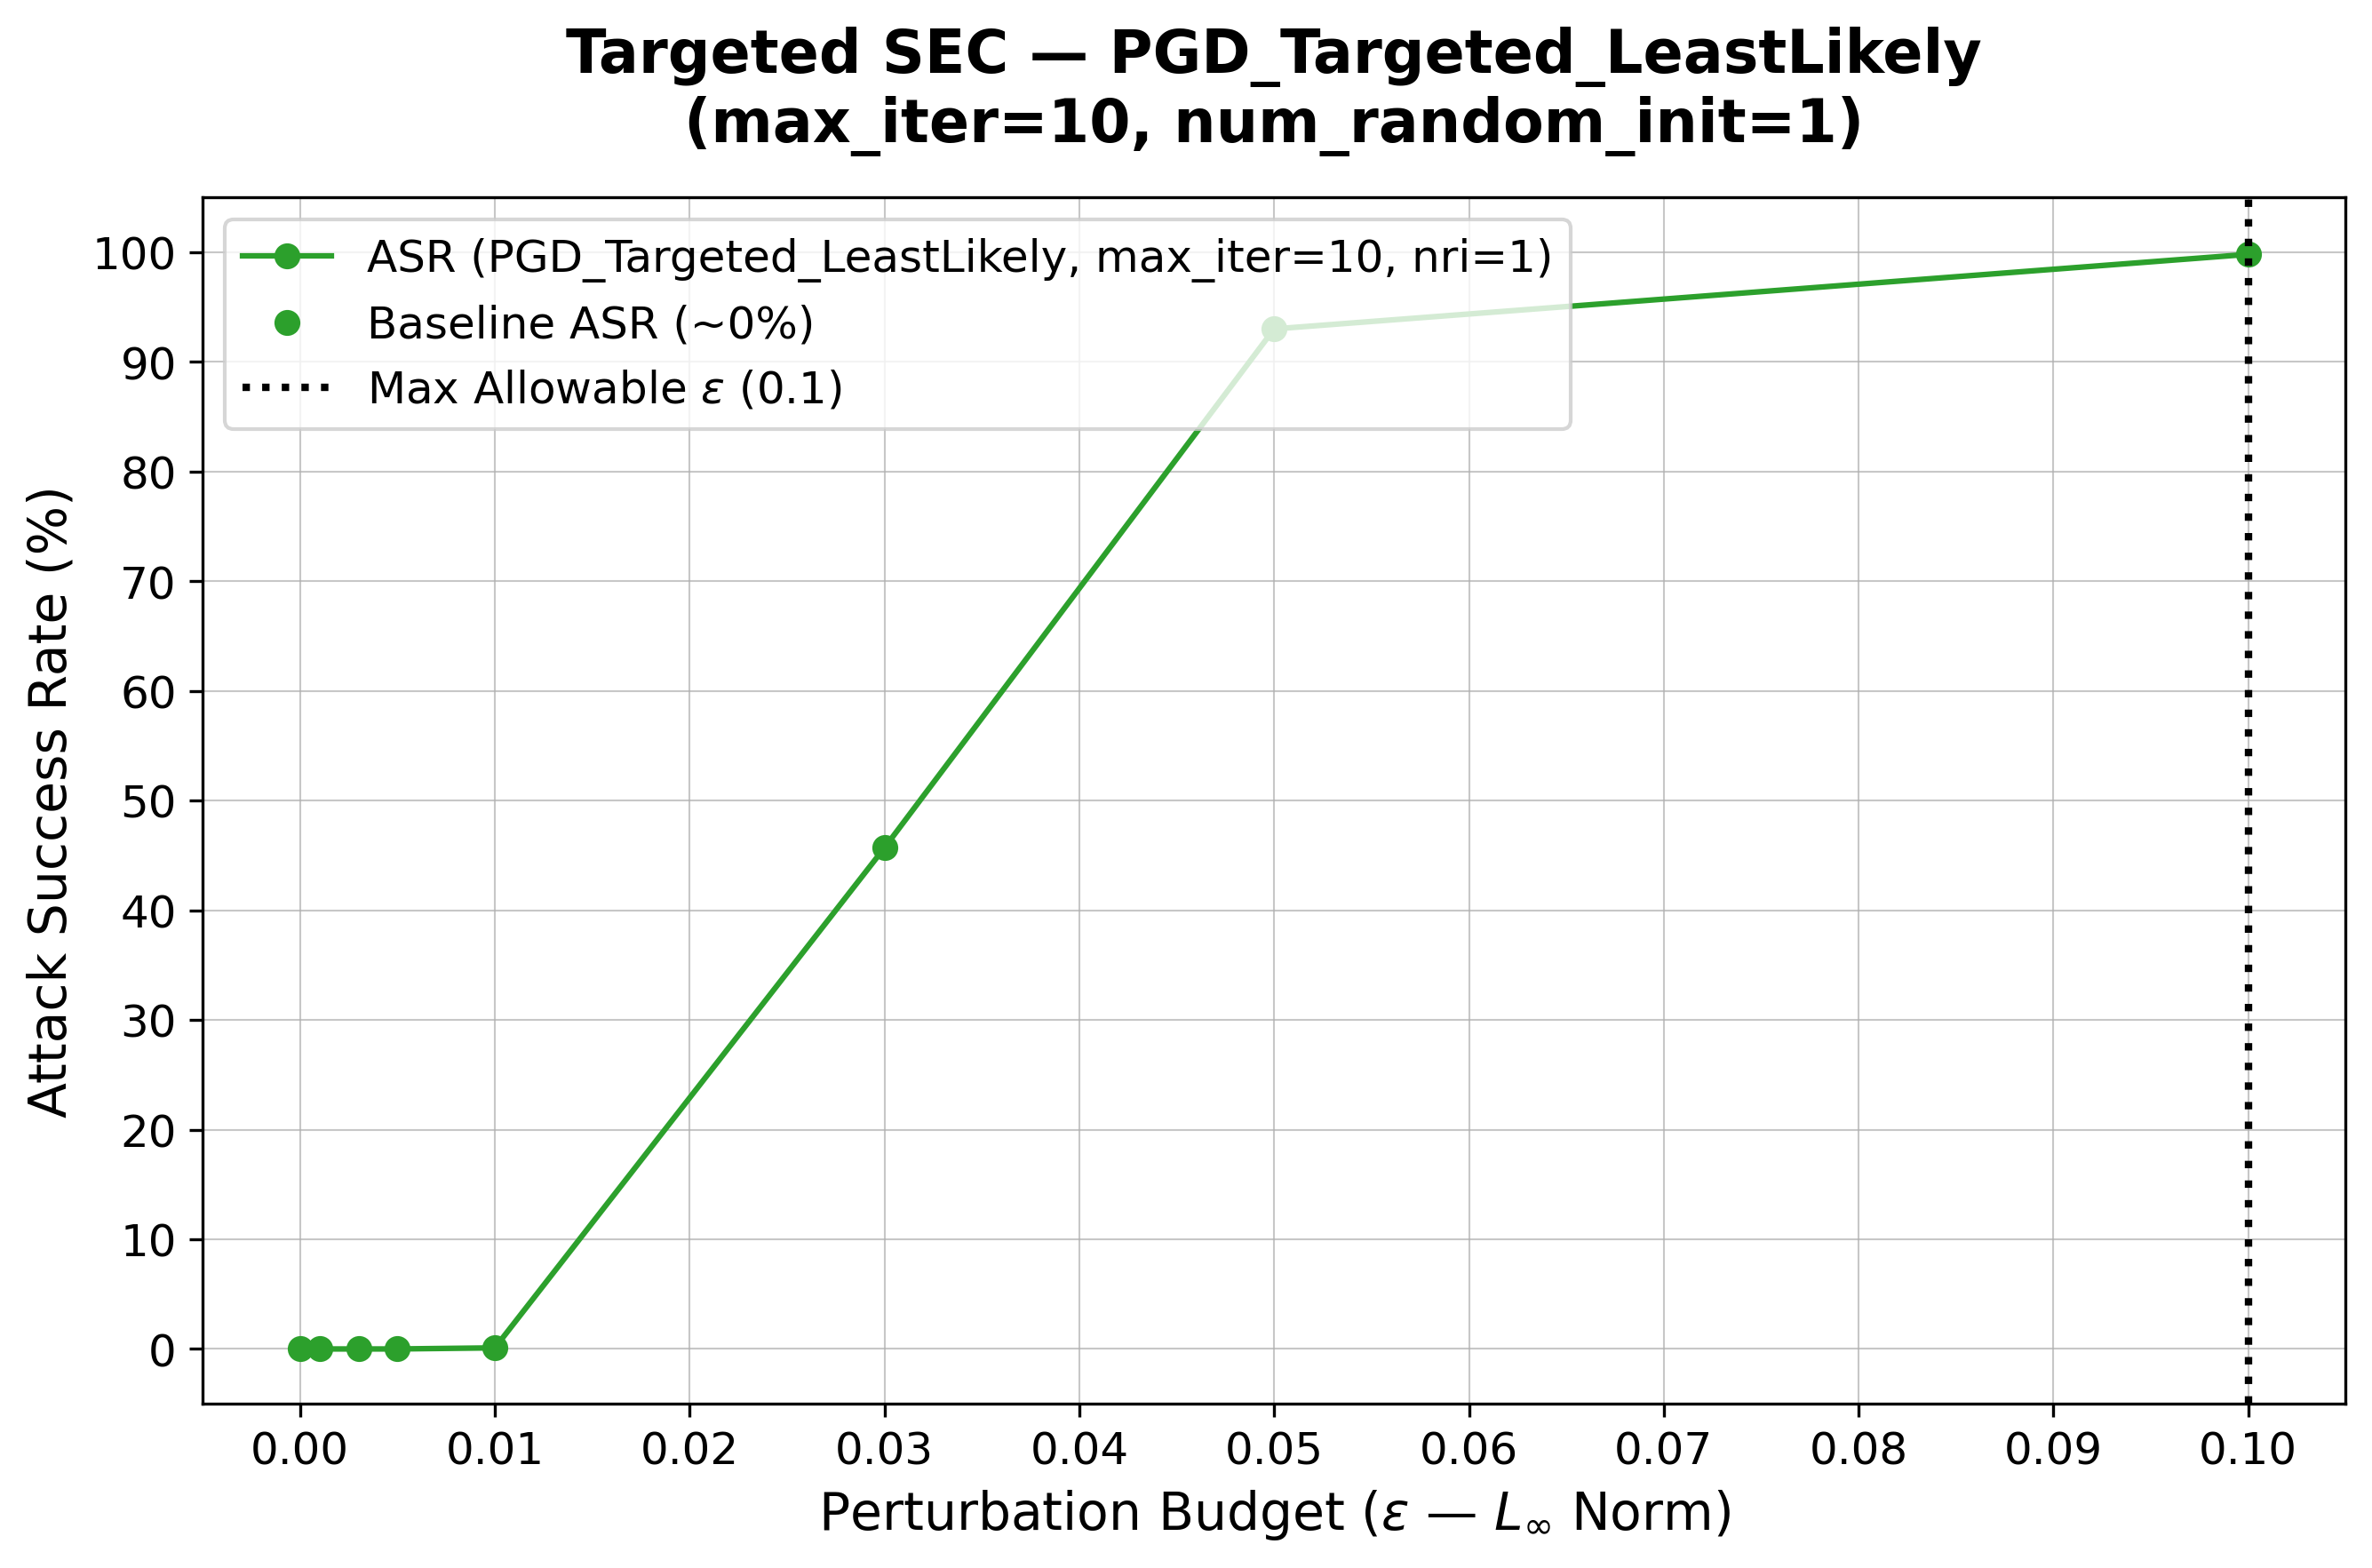
\includegraphics[width=\textwidth]{PGD_Error_specific/LL/PGD_Targeted_LeastLikely_nri1_iter10_SEC.png}
        \caption{\texttt{max_iter} = 10}
        \label{fig:PGD_LL_nri1_iter10}
    \end{subfigure}
    \hfill
    % Sotto-figura 4
    \begin{subfigure}[b]{0.45\textwidth}
        \centering
        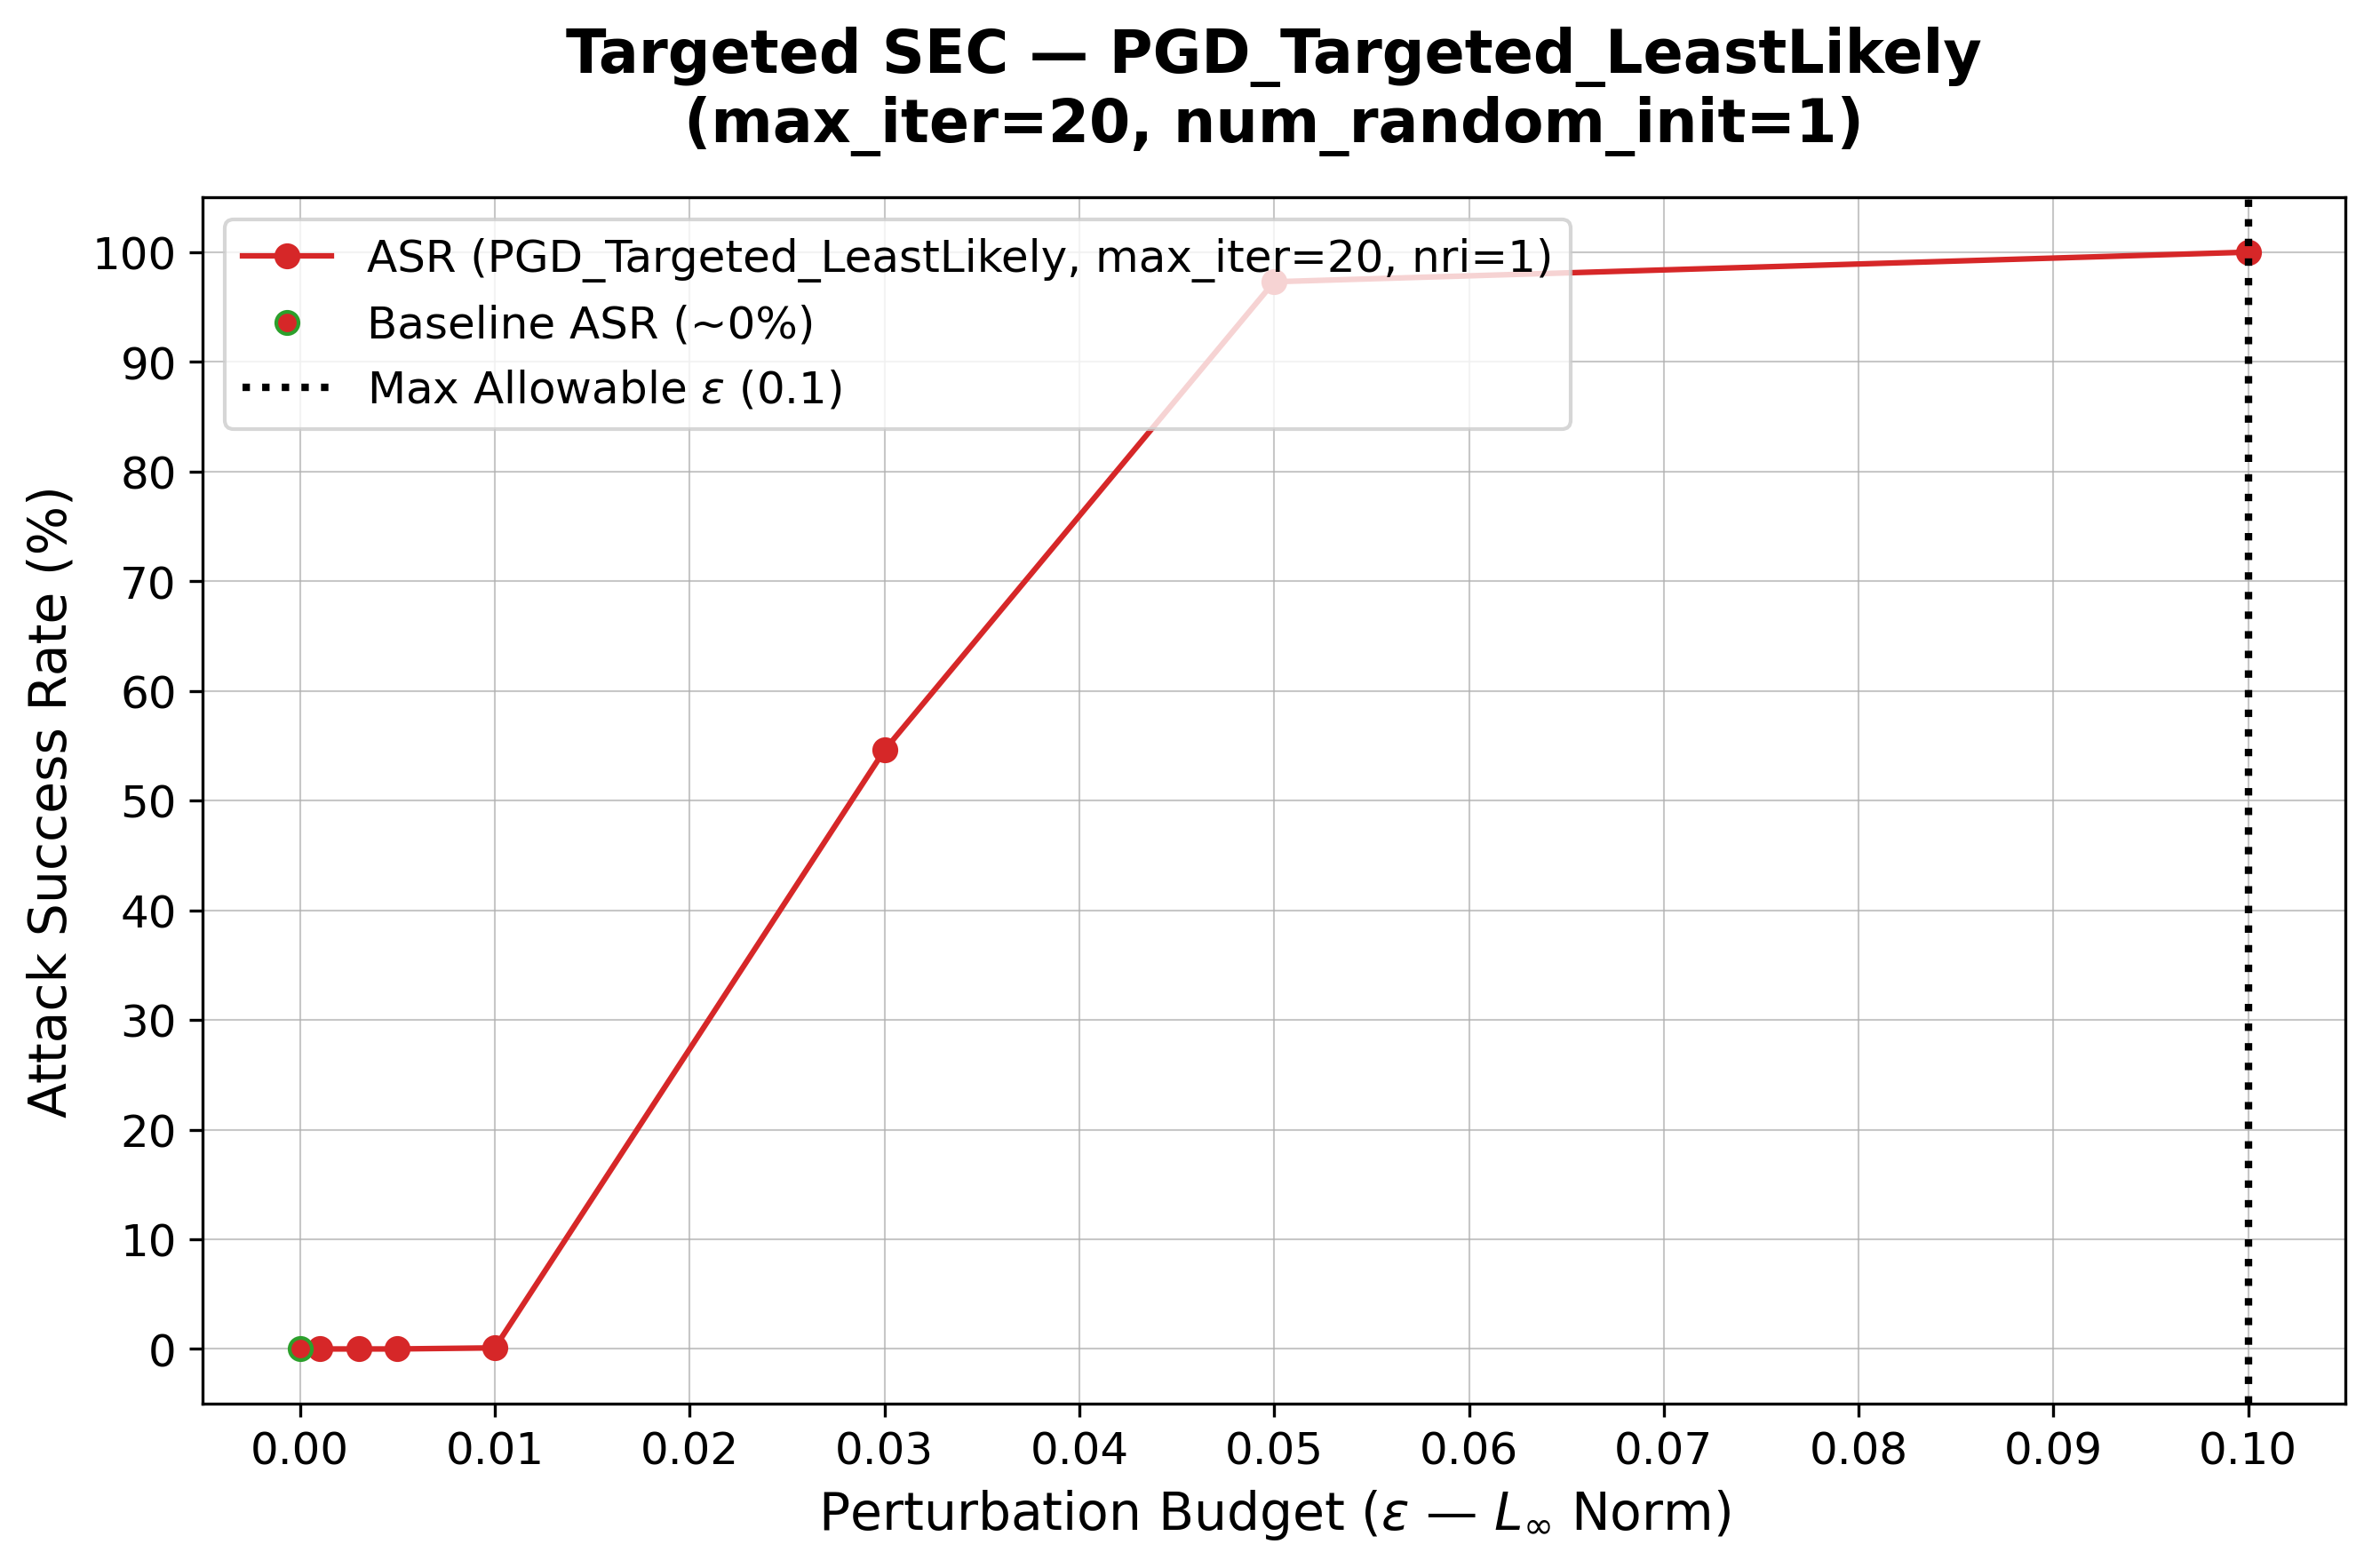
\includegraphics[width=\textwidth]{PGD_Error_specific/LL/PGD_Targeted_LeastLikely_nri1_iter20_SEC.png}
        \caption{\texttt{max_iter} = 20}
        \label{fig:PGD_LL_nri1_iter20}
    \end{subfigure}
    \vspace{1em} % Spazio verticale tra le righe di immagini
    % Sotto-figura 5
    \begin{subfigure}[b]{0.45\textwidth}
        \centering
        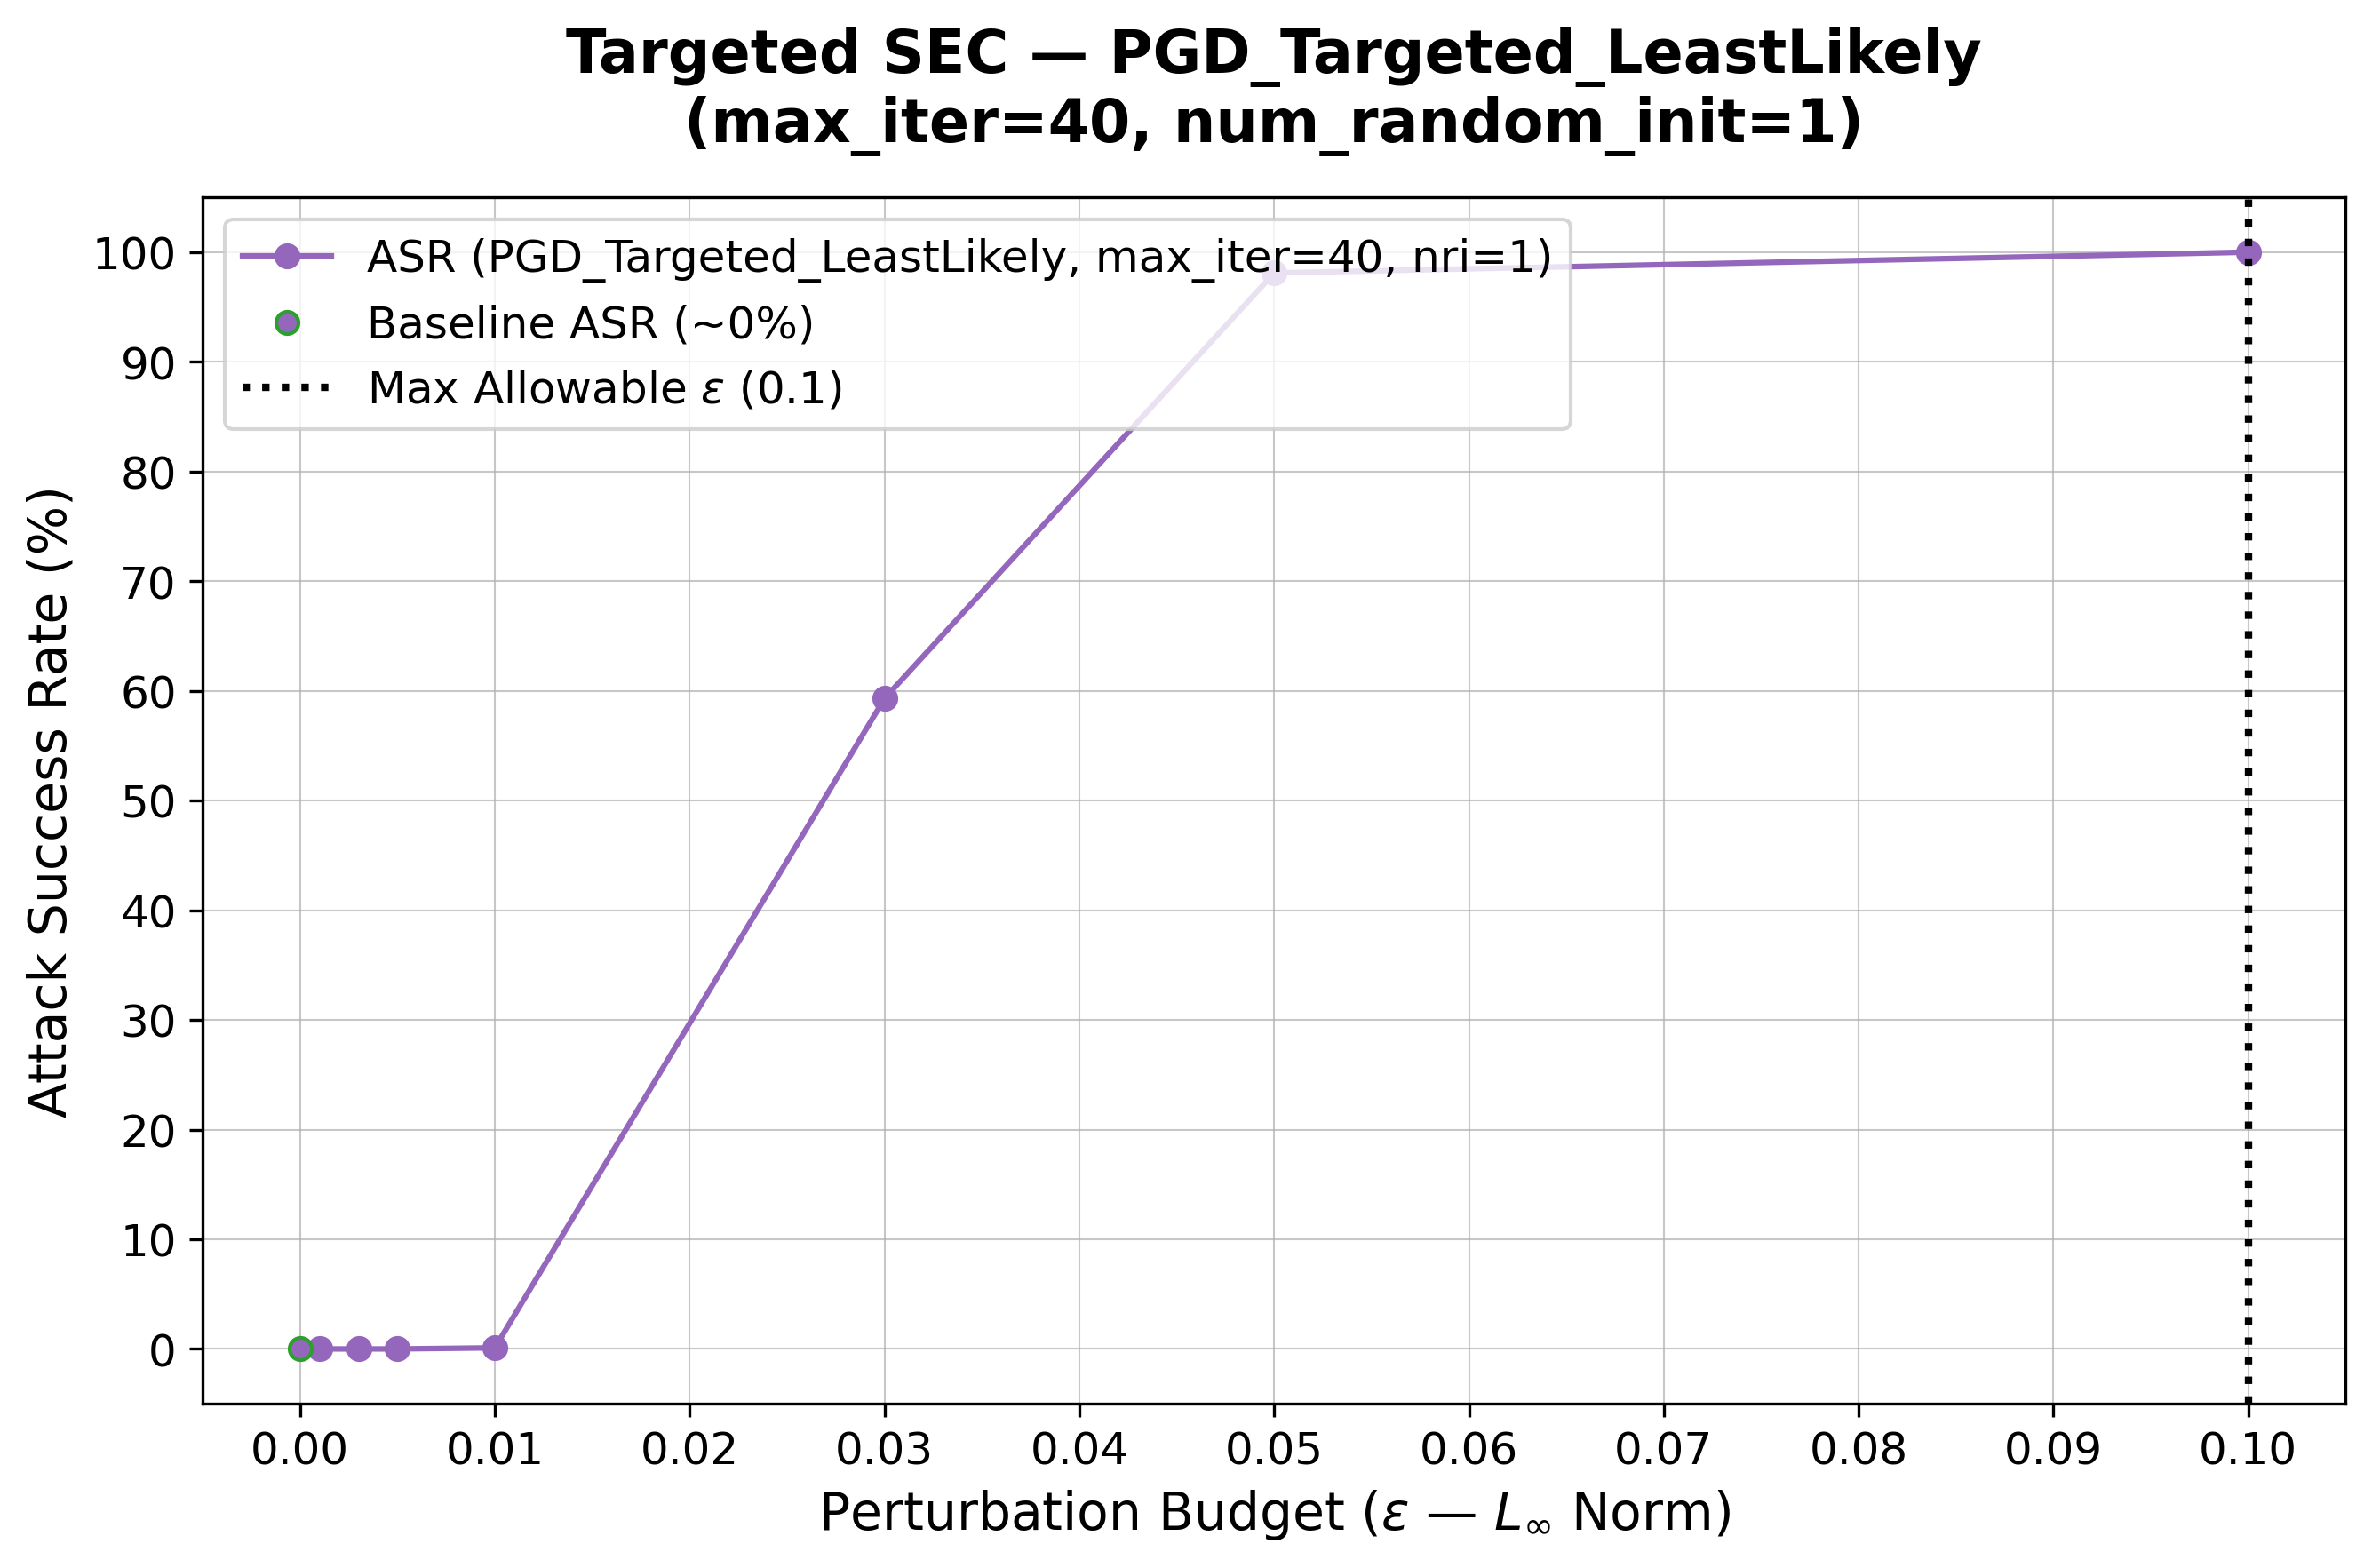
\includegraphics[width=\textwidth]{PGD_Error_specific/LL/PGD_Targeted_LeastLikely_nri1_iter40_SEC.png}
        \caption{\texttt{max_iter} = 40}
        \label{fig:PGD_LL_nri1_iter40}
    \end{subfigure}
    \caption{PGD Least Likely - Iterazioni a confronto per \texttt{nri} = 1}
    \label{fig:PGD_LL_iterations_nri1}
\end{figure}

% -- SEC NRI = 3 --
\begin{figure}[H]
    \centering
    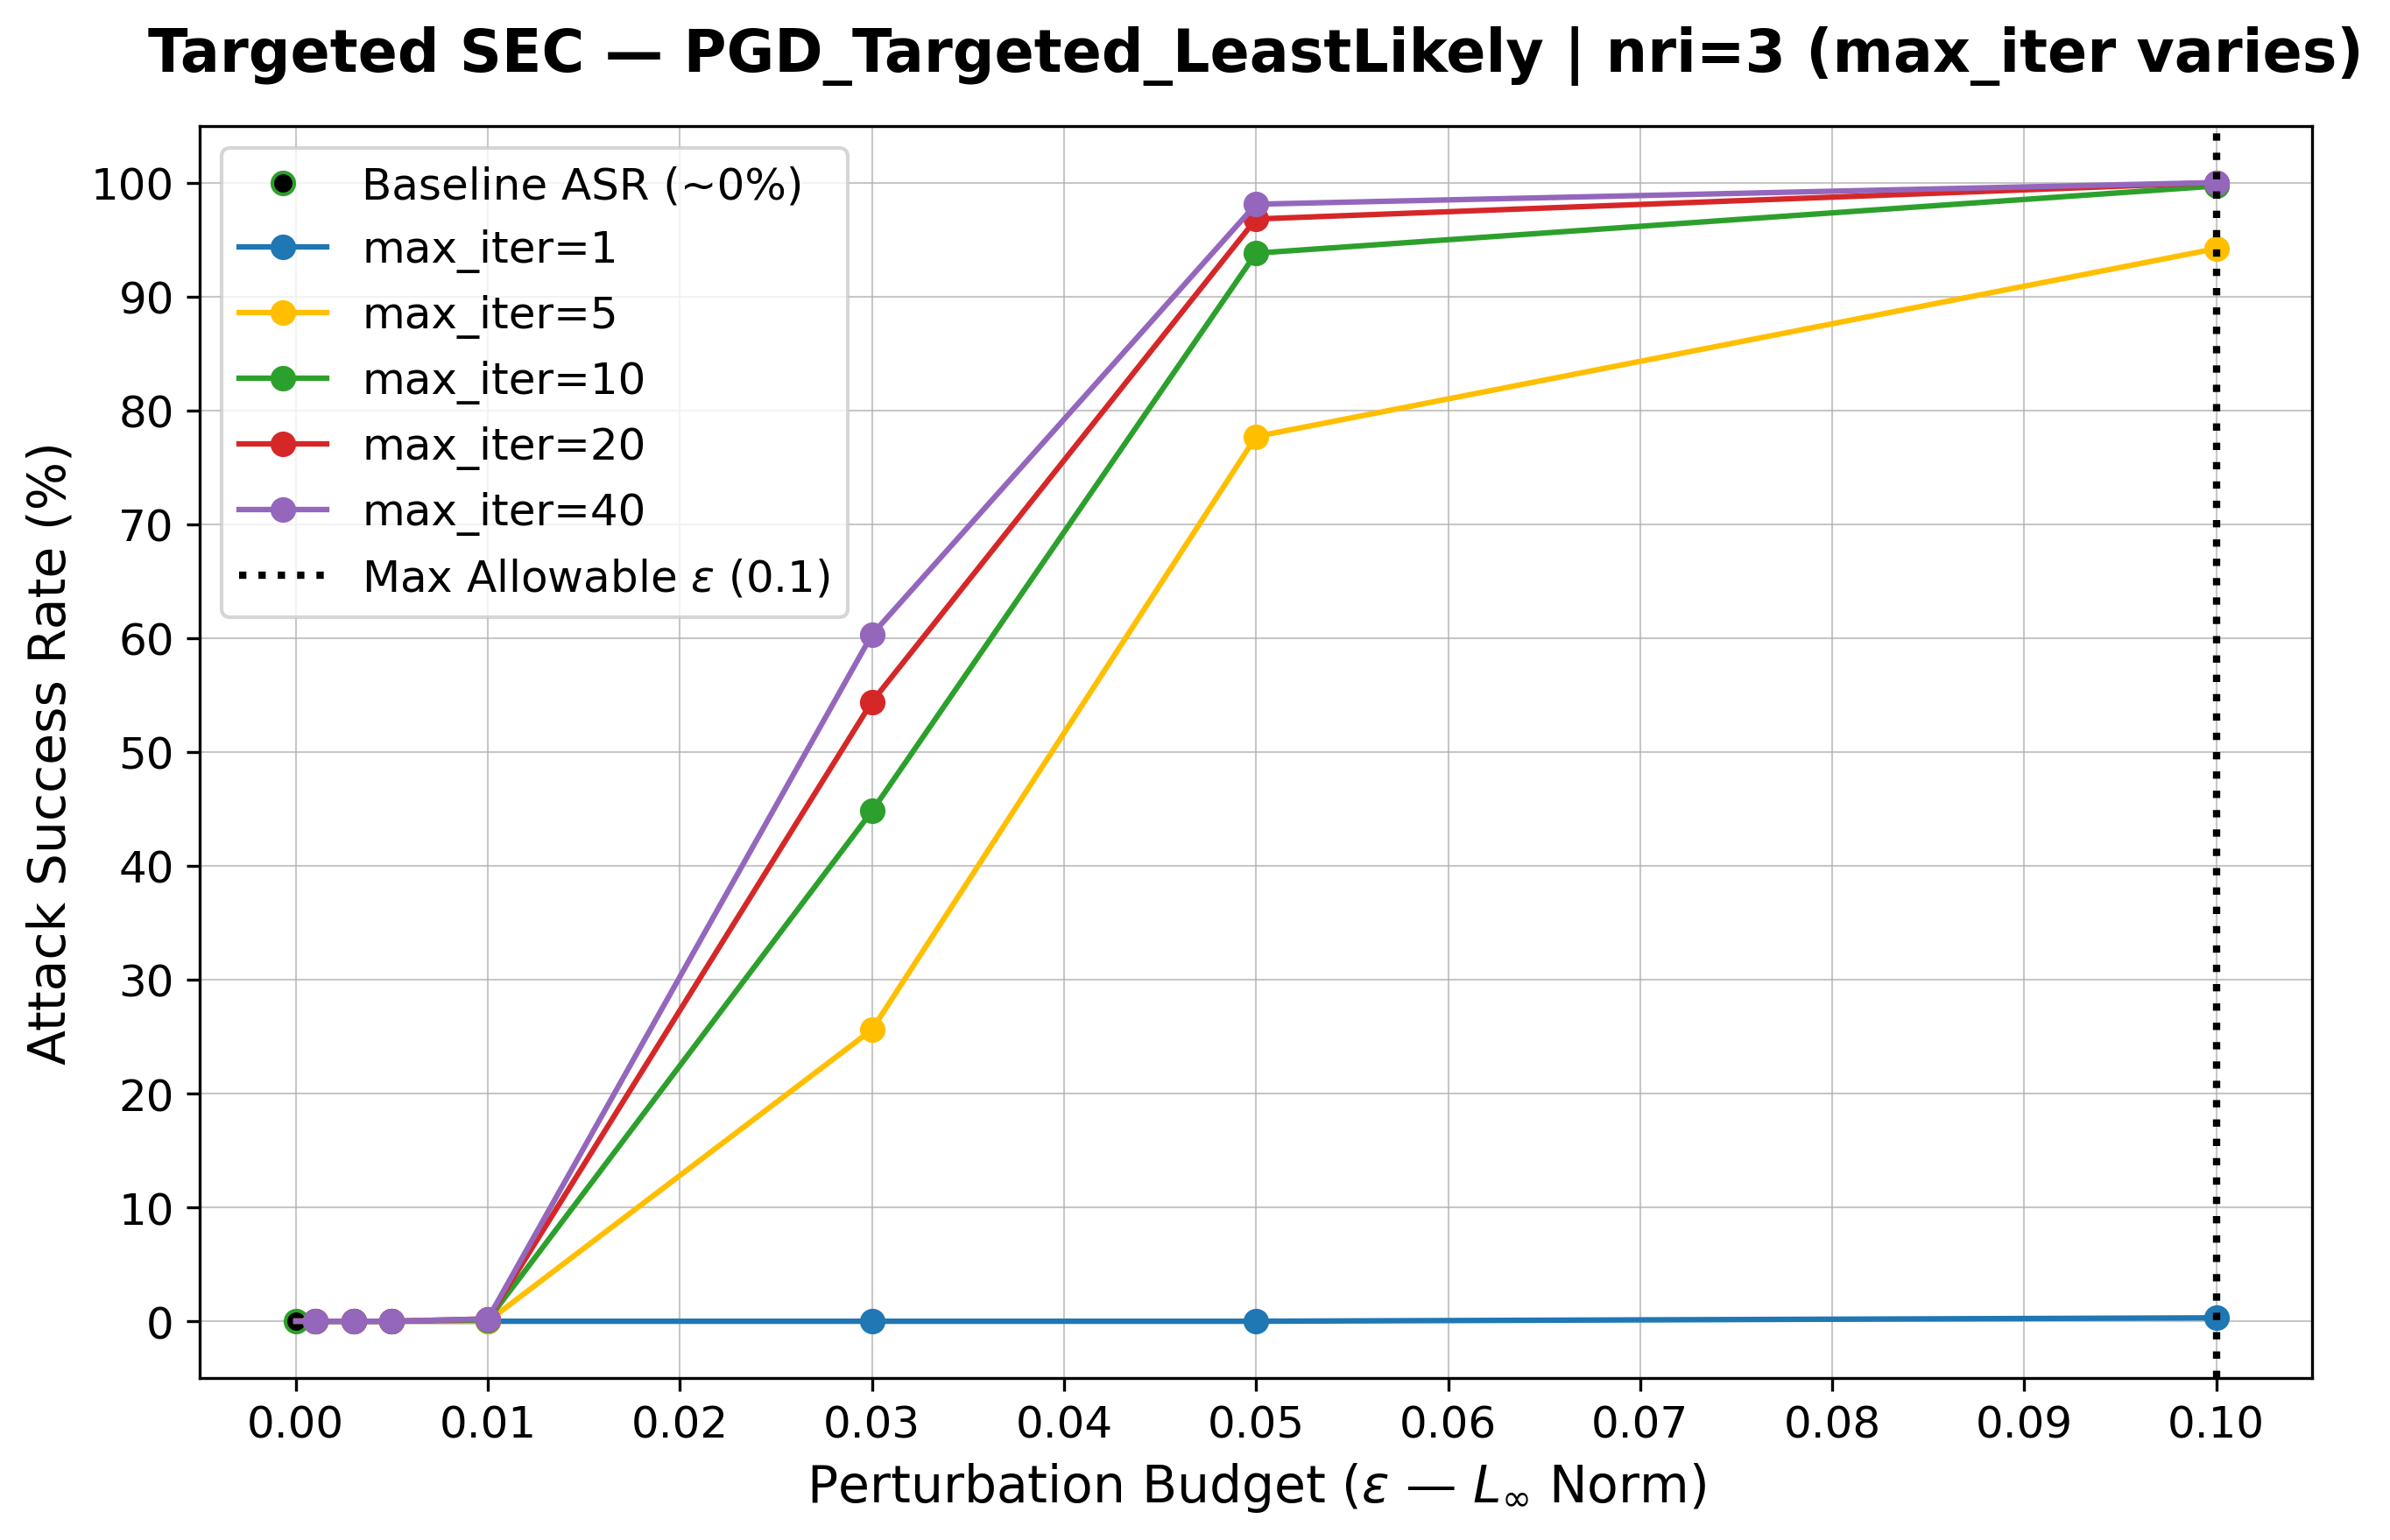
\includegraphics[width=0.5\linewidth]{PGD_Error_specific/LL/PGD_Targeted_LeastLikely_nri3_comparative_maxiter_SEC.png}  
    \caption{PGD Least Likely SEC con nri = 3}
    \label{fig:PGD_LL_SEC_nri3}
\end{figure}

% -- SOTTO GRAFICI PER NRI = 3
\begin{figure}[H]
    \centering
    % Sotto-figura 1
    \begin{subfigure}[b]{0.45\textwidth}
        \centering
        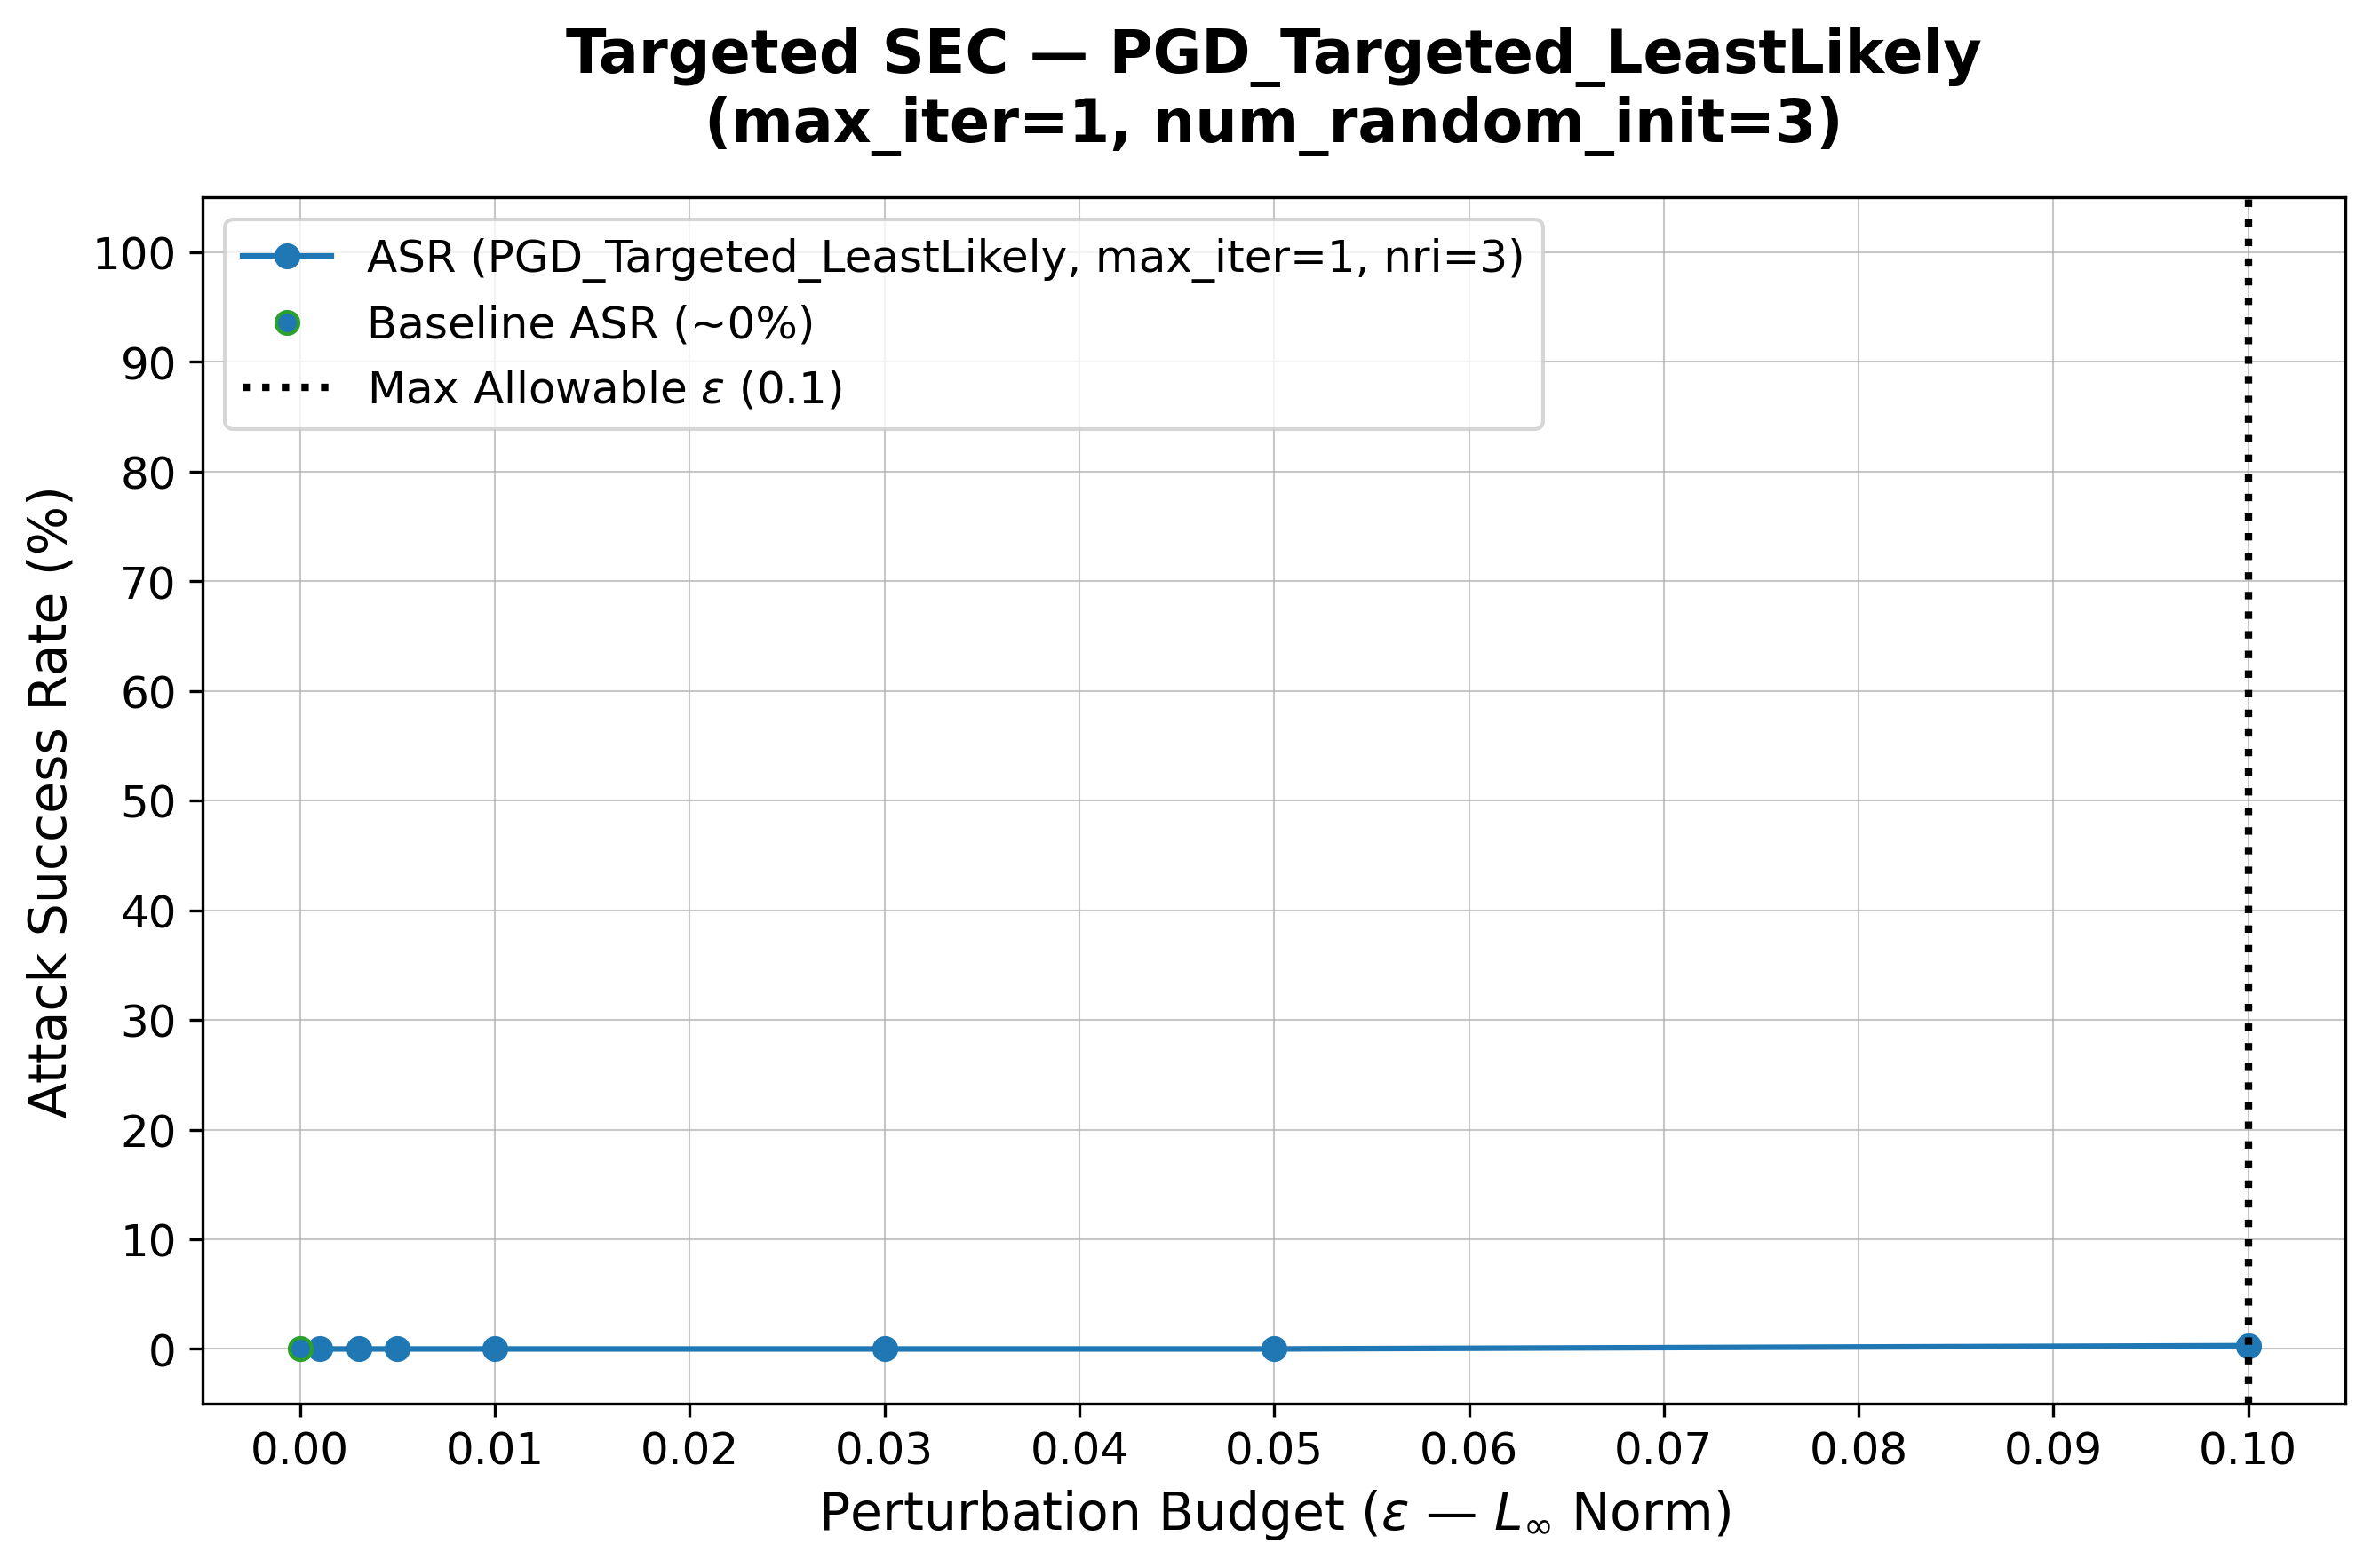
\includegraphics[width=\textwidth]{PGD_Error_specific/LL/PGD_Targeted_LeastLikely_nri3_iter1_SEC.png}
        \caption{\texttt{max_iter} = 1}
        \label{fig:PGD_LL_nri3_iter1}
    \end{subfigure}
    \hfill
    % Sotto-figura 2
    \begin{subfigure}[b]{0.45\textwidth}
        \centering
        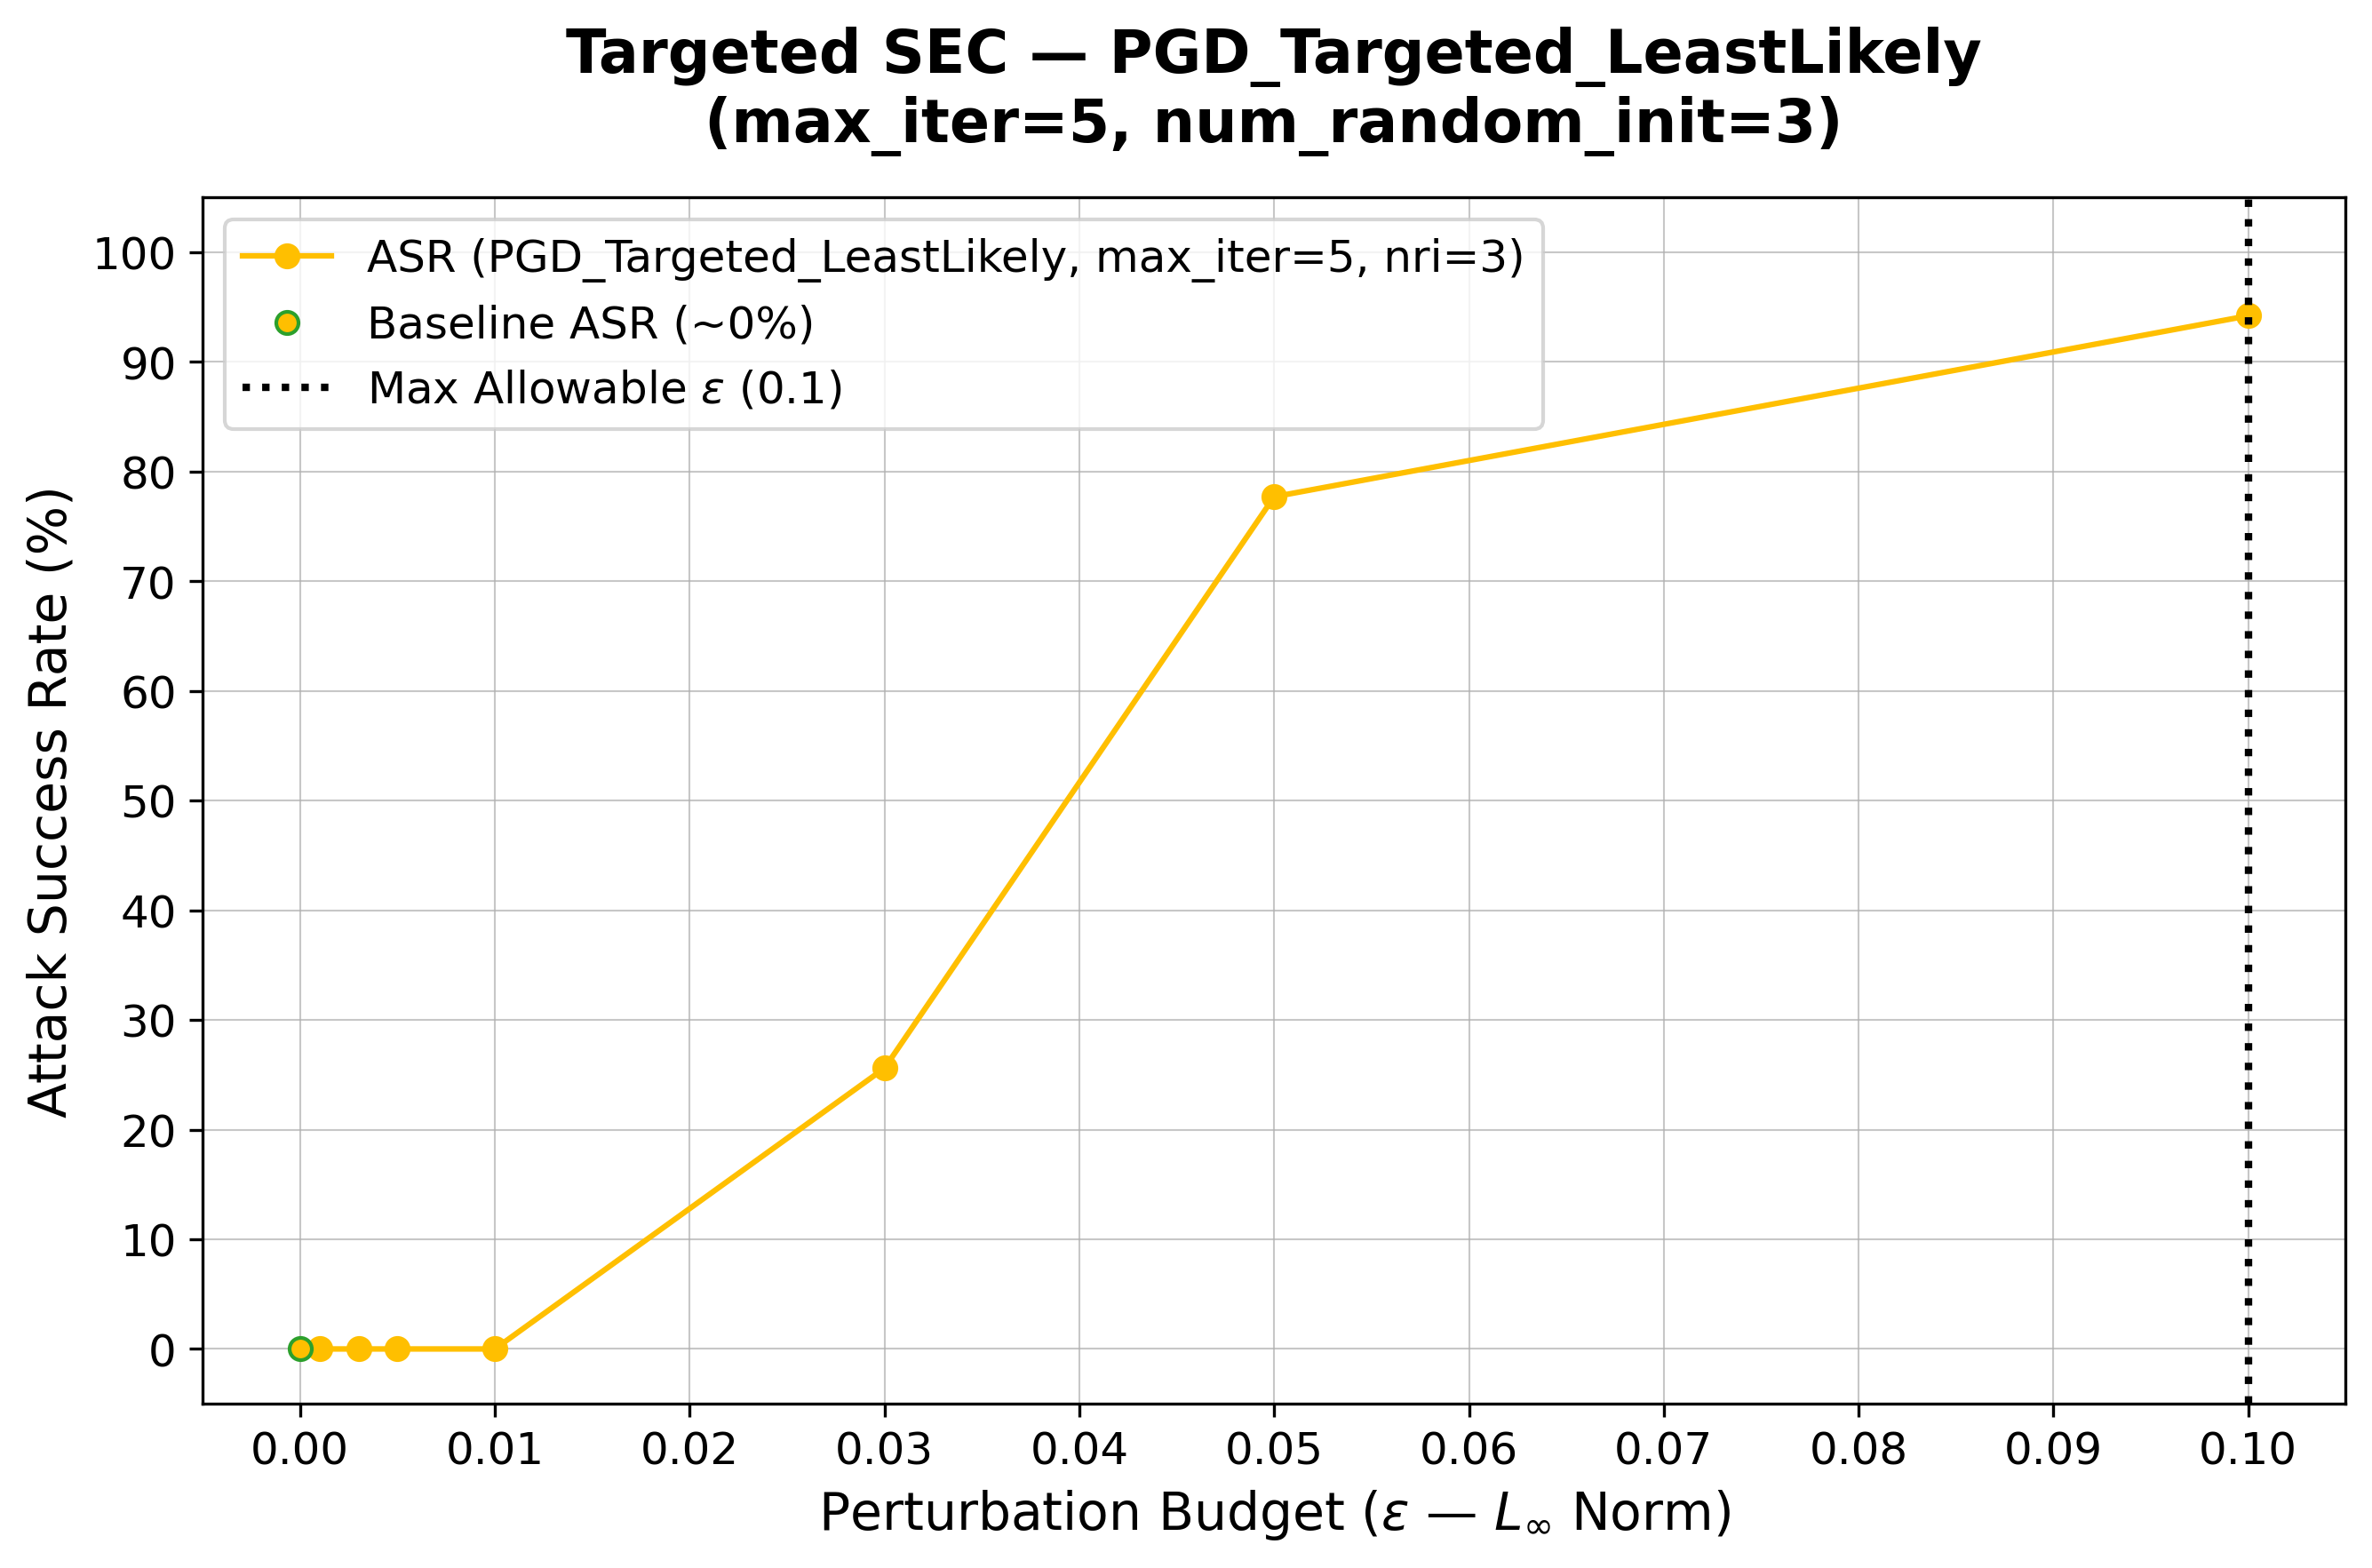
\includegraphics[width=\textwidth]{PGD_Error_specific/LL/PGD_Targeted_LeastLikely_nri3_iter5_SEC.png}
        \caption{\texttt{max_iter} = 5}
        \label{fig:PGD_LL_nri3_iter5}
    \end{subfigure}

    \vspace{1em} % Spazio verticale tra le righe di immagini
    % Sotto-figura 3
    \begin{subfigure}[b]{0.45\textwidth}
        \centering
        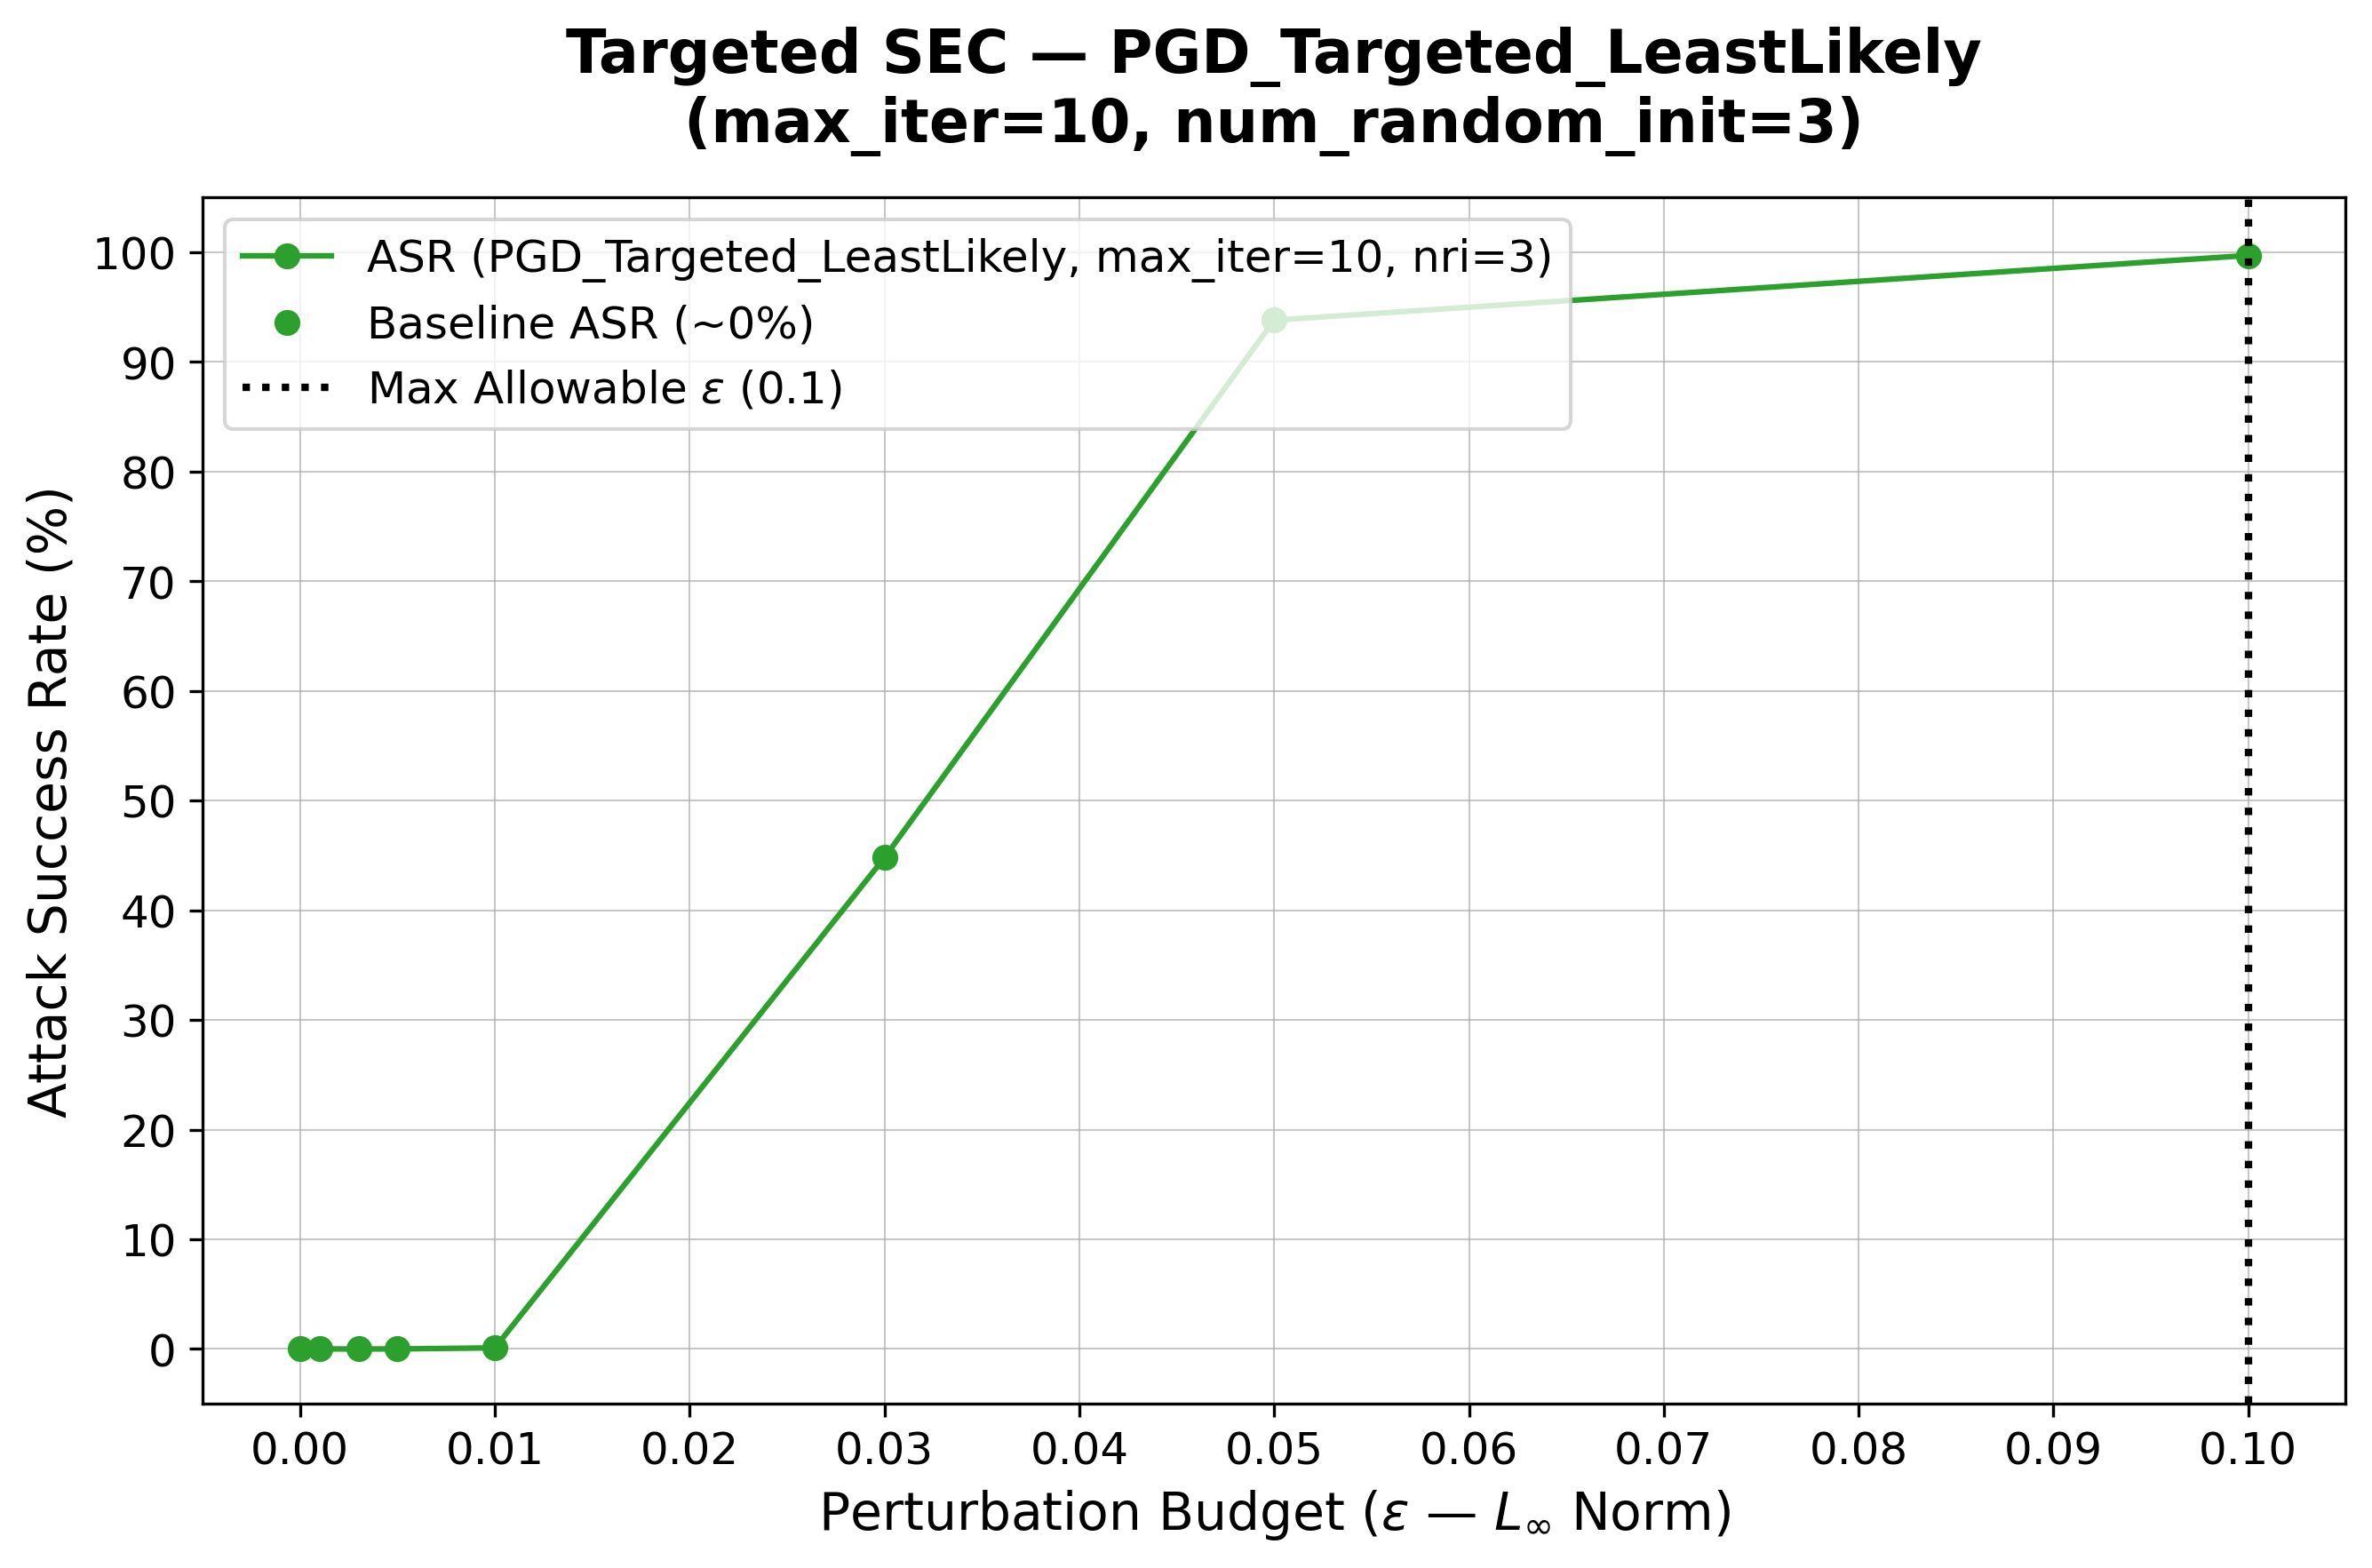
\includegraphics[width=\textwidth]{PGD_Error_specific/LL/PGD_Targeted_LeastLikely_nri3_iter10_SEC.png}
        \caption{\texttt{max_iter} = 10}
        \label{fig:PGD_LL_nri3_iter10}
    \end{subfigure}
    \hfill
    % Sotto-figura 4
    \begin{subfigure}[b]{0.45\textwidth}
        \centering
        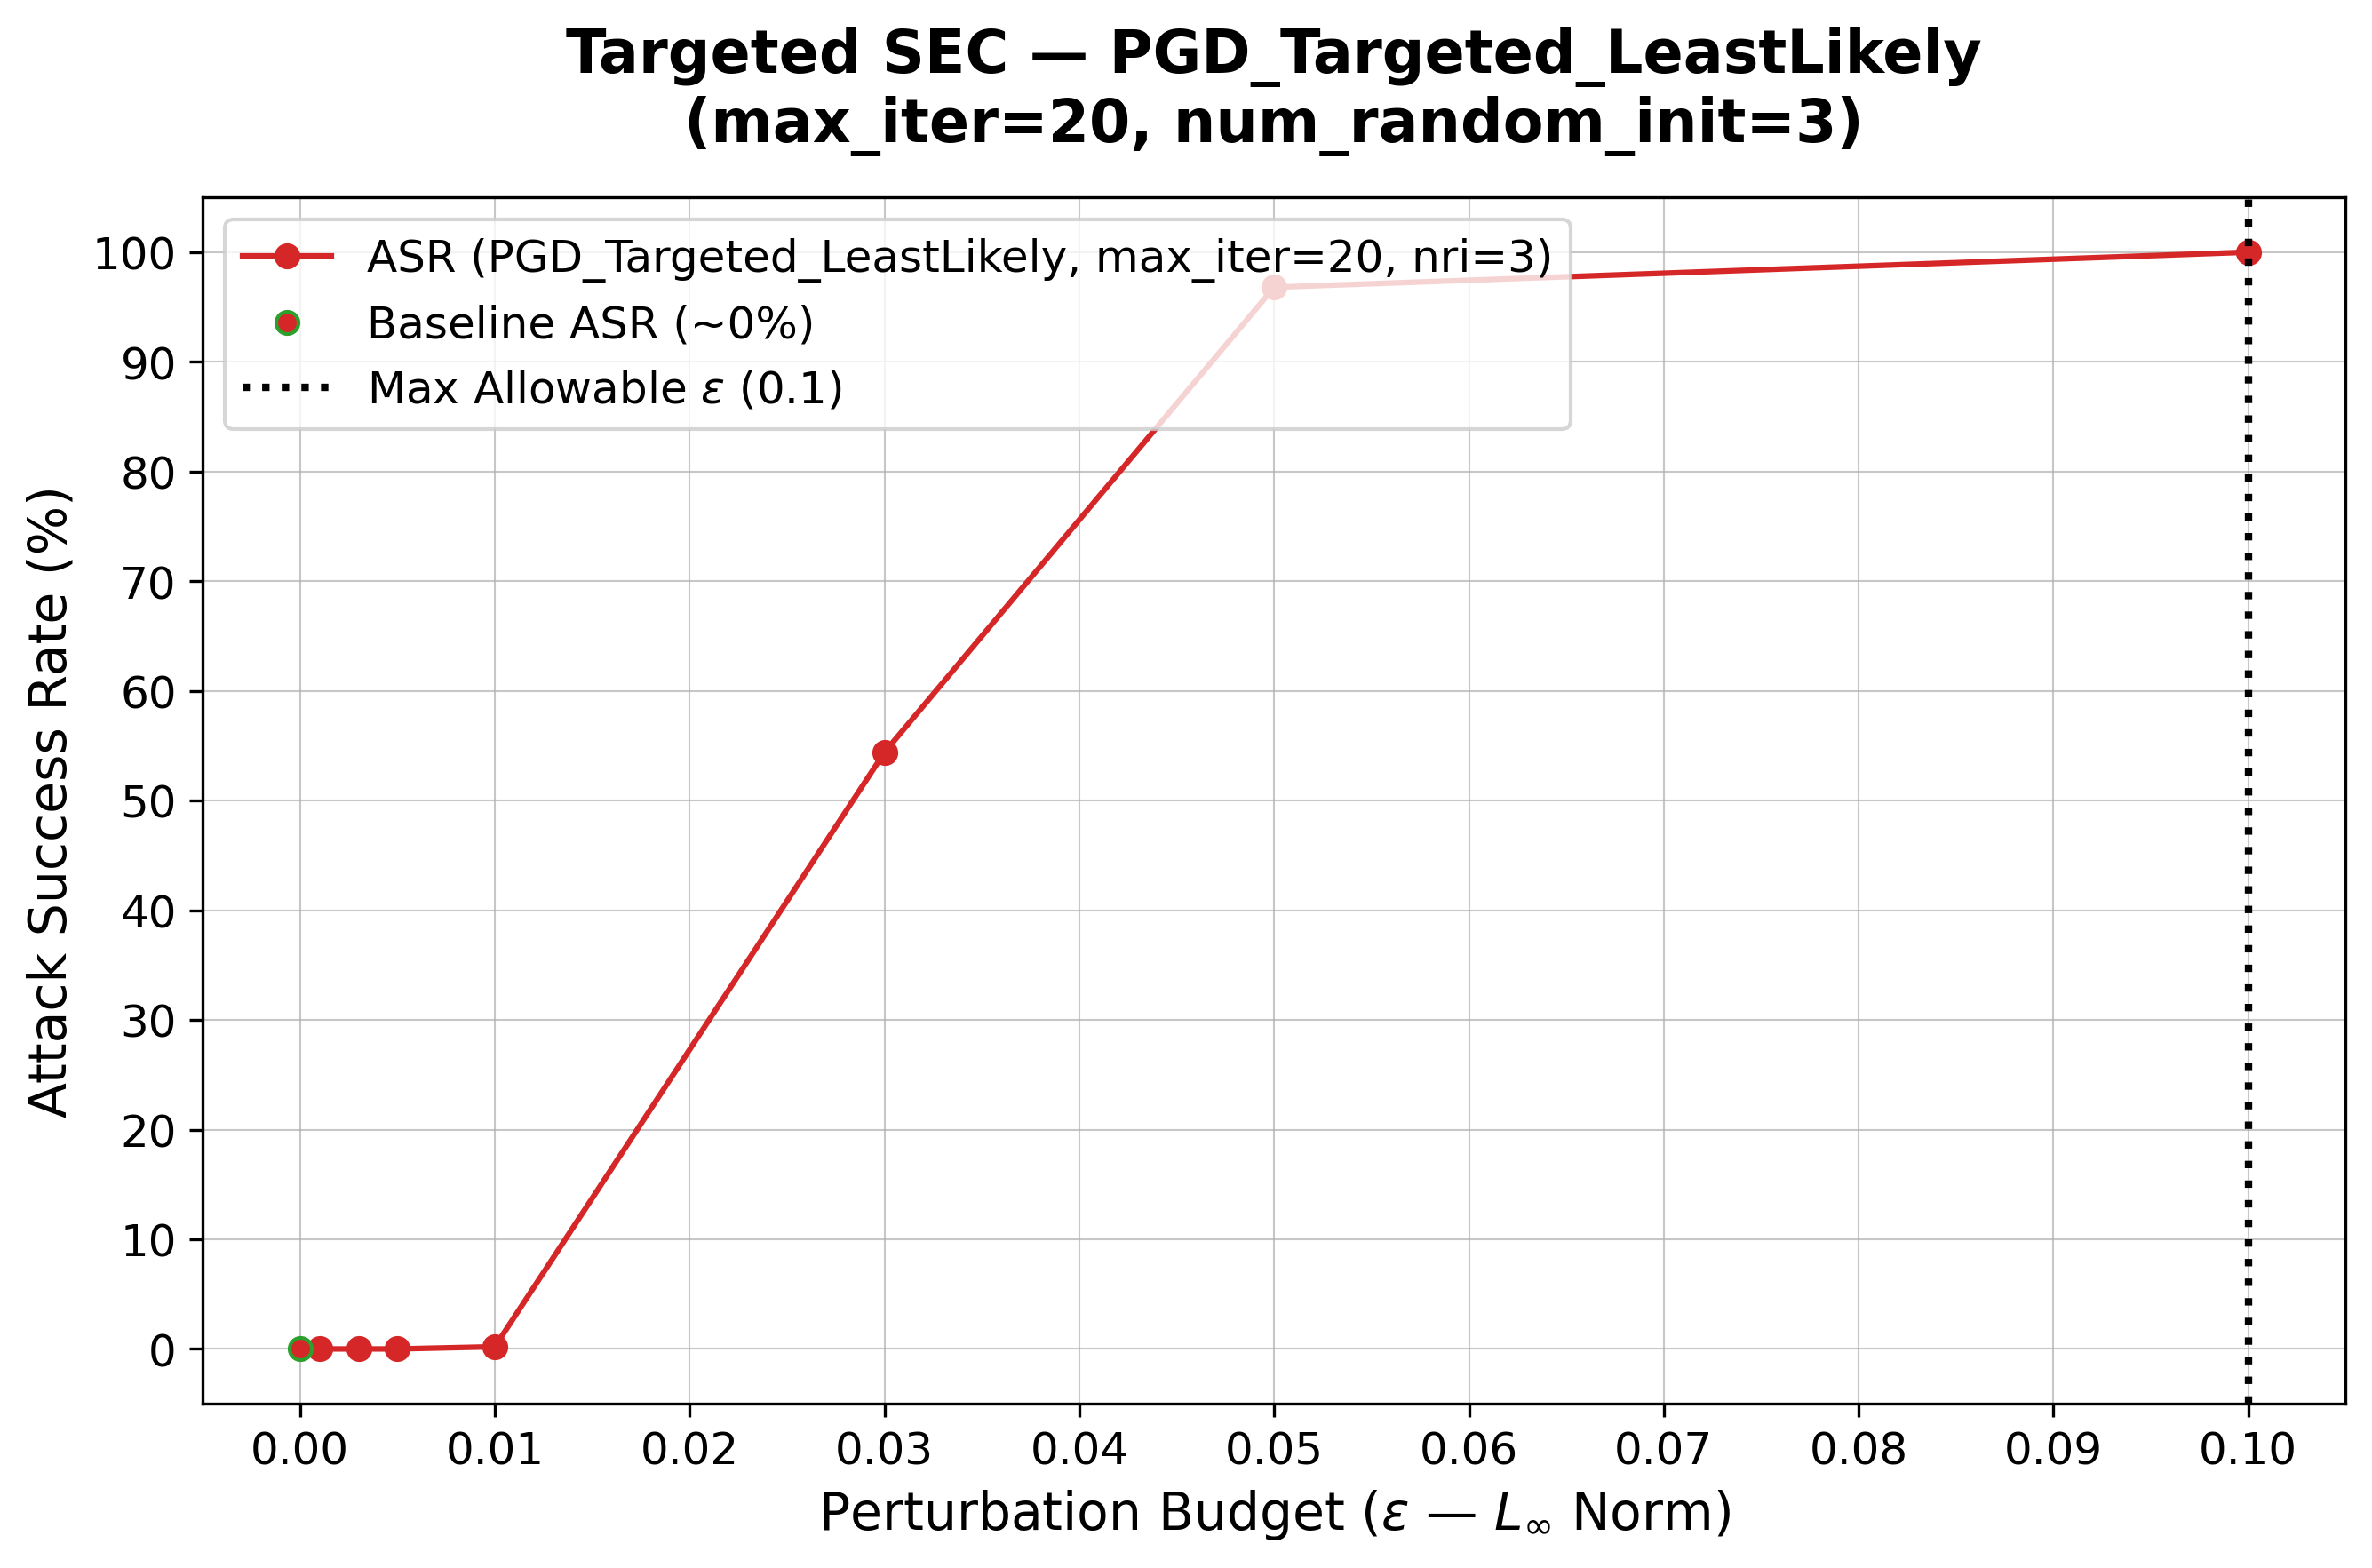
\includegraphics[width=\textwidth]{PGD_Error_specific/LL/PGD_Targeted_LeastLikely_nri3_iter20_SEC.png}
        \caption{\texttt{max_iter} = 20}
        \label{fig:PGD_LL_nri3_iter20}
    \end{subfigure}
    \vspace{1em} % Spazio verticale tra le righe di immagini
    % Sotto-figura 5
    \begin{subfigure}[b]{0.45\textwidth}
        \centering
        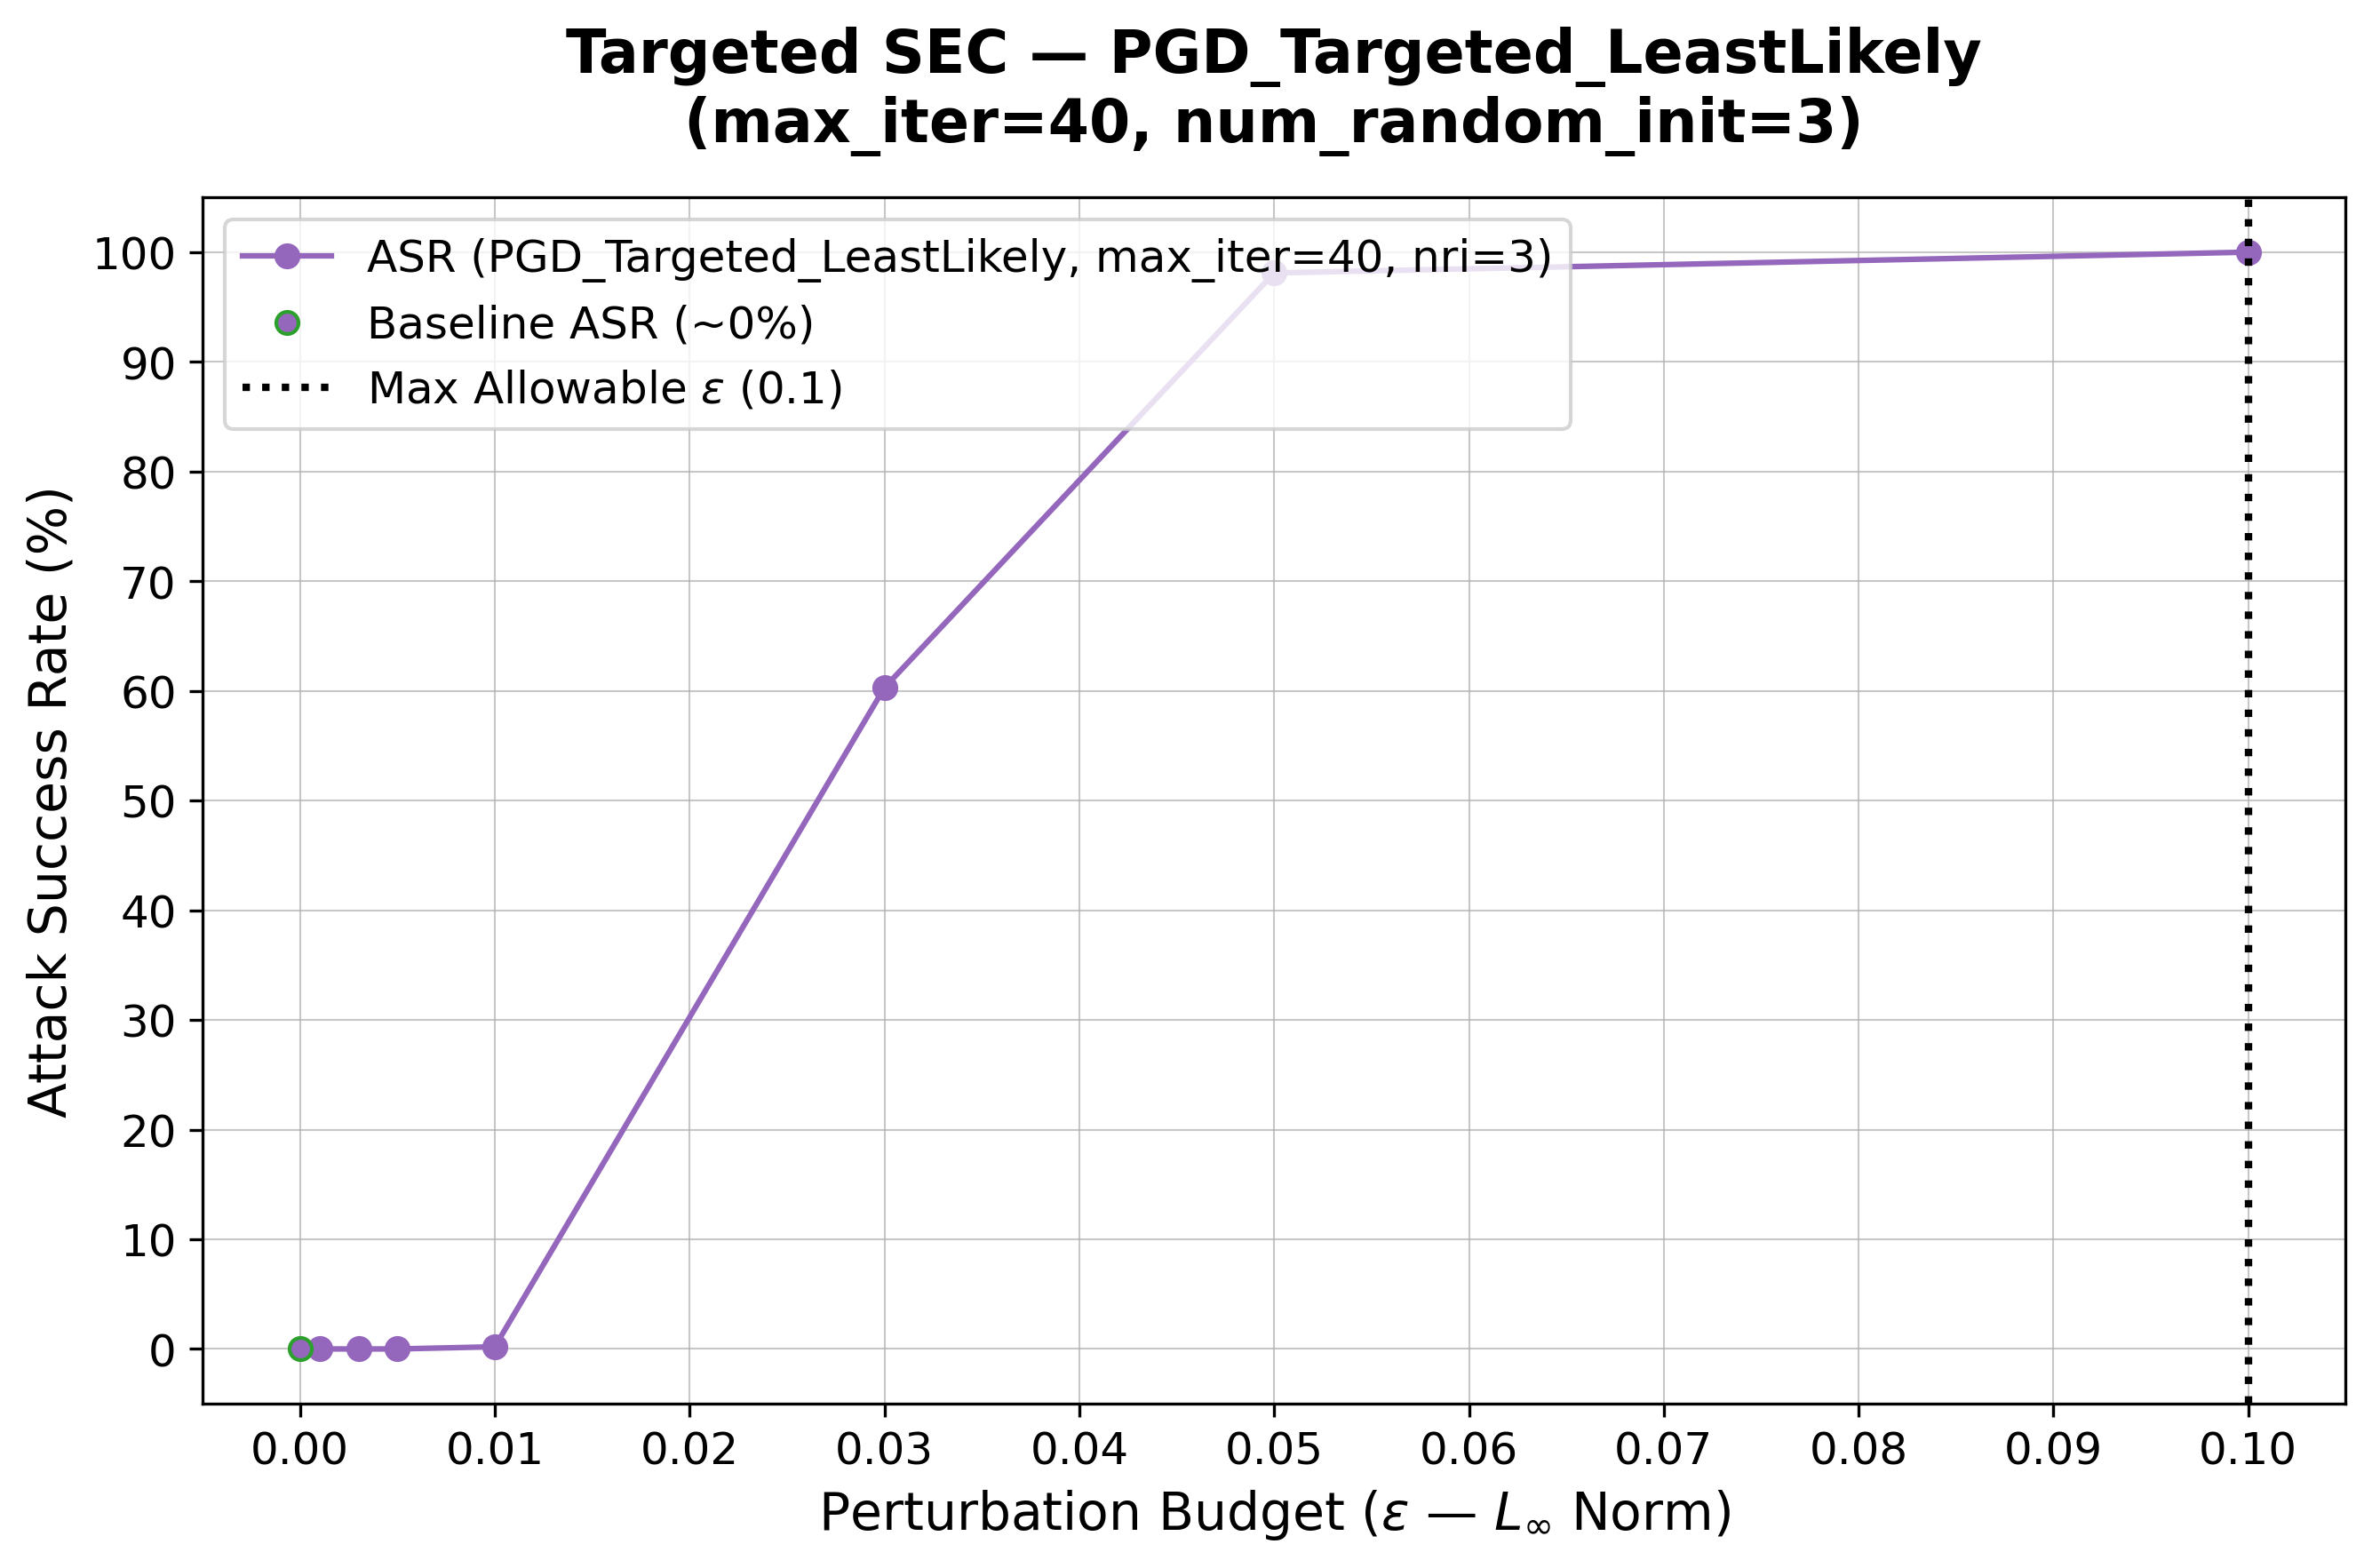
\includegraphics[width=\textwidth]{PGD_Error_specific/LL/PGD_Targeted_LeastLikely_nri3_iter40_SEC.png}
        \caption{\texttt{max_iter} = 40}
        \label{fig:PGD_LL_nri3_iter40}
    \end{subfigure}
    \caption{PGD Least Likely - Iterazioni a confronto per \texttt{nri} = 3}
    \label{fig:PGD_LL_iterations_nri3}
\end{figure}

% -- SEC NRI = 5 --
\begin{figure}[H]
    \centering
    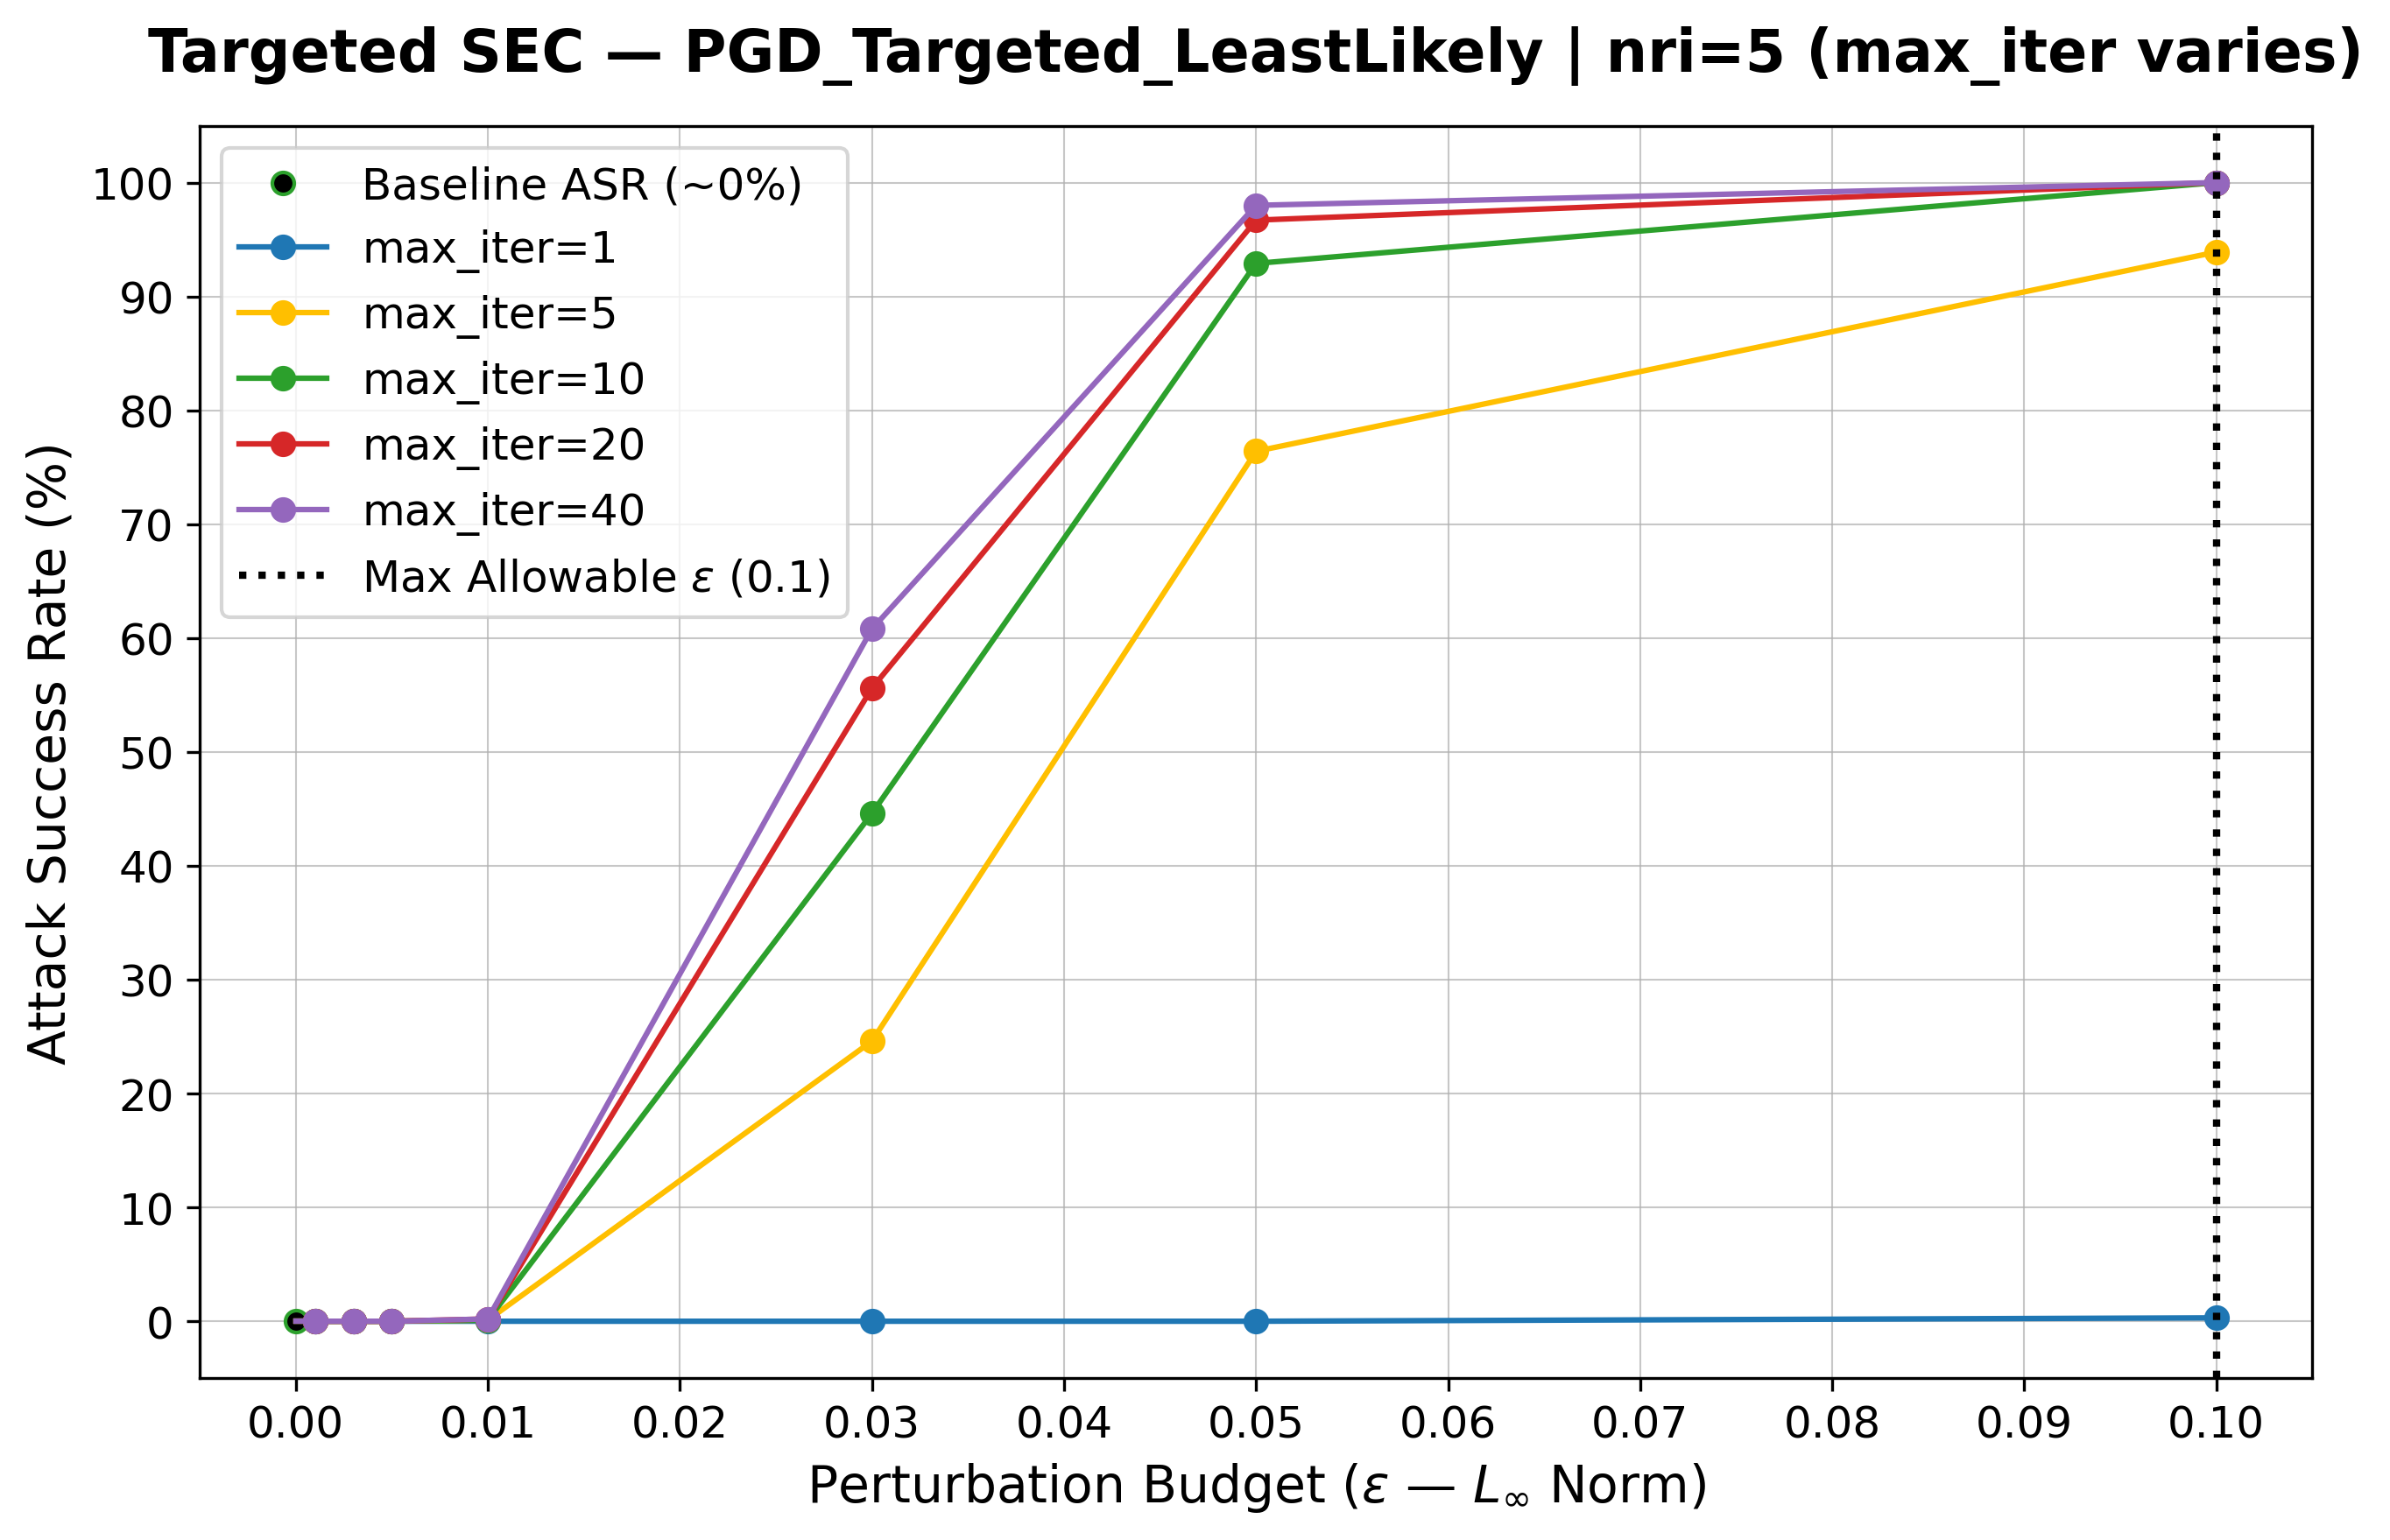
\includegraphics[width=0.5\linewidth]{PGD_Error_specific/LL/PGD_Targeted_LeastLikely_nri5_comparative_maxiter_SEC.png}
    \caption{PGD Least Likely SEC con nri = 5}
    \label{fig:PGD_LL_SEC_nri5}
\end{figure}    

% -- SOTTO GRAFICI PER NRI = 5
\begin{figure}[H]
    \centering
    % Sotto-figura 1
    \begin{subfigure}[b]{0.45\textwidth}
        \centering
        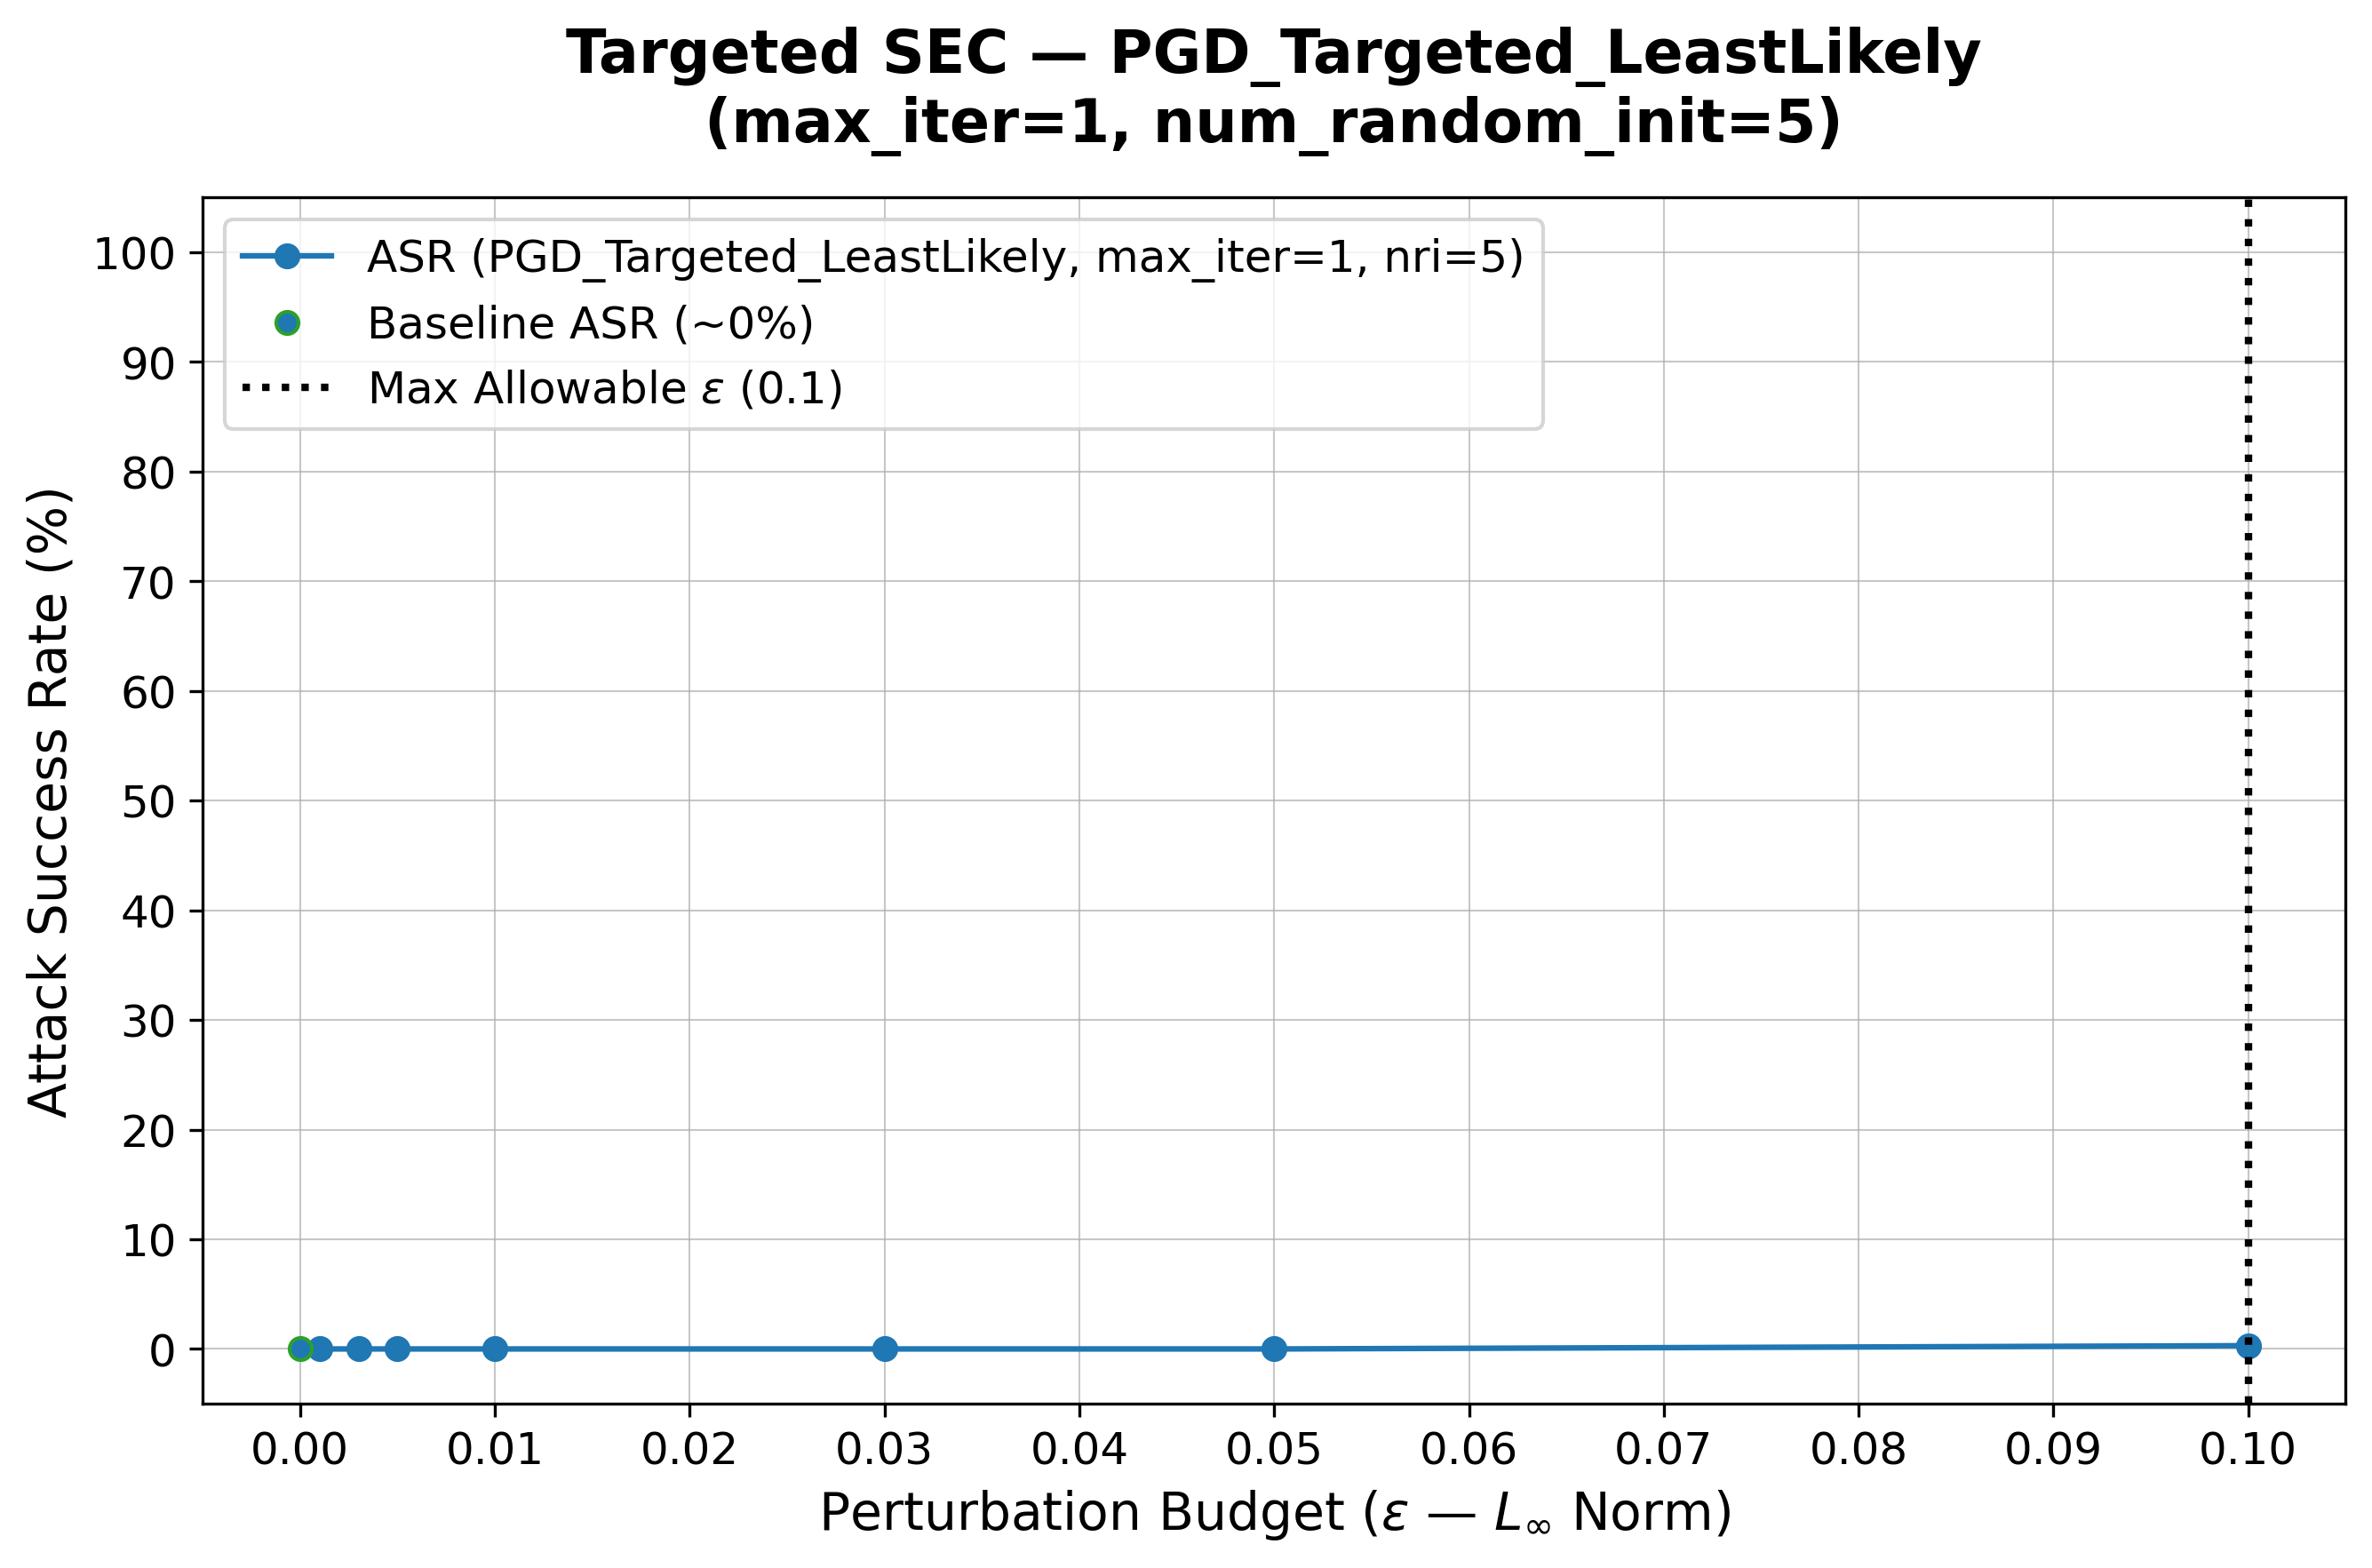
\includegraphics[width=\textwidth]{PGD_Error_specific/LL/PGD_Targeted_LeastLikely_nri5_iter1_SEC.png}
        \caption{\texttt{max_iter} = 1}
        \label{fig:PGD_LL_nri5_iter1}
    \end{subfigure}
    \hfill
    % Sotto-figura 2
    \begin{subfigure}[b]{0.45\textwidth}
        \centering
        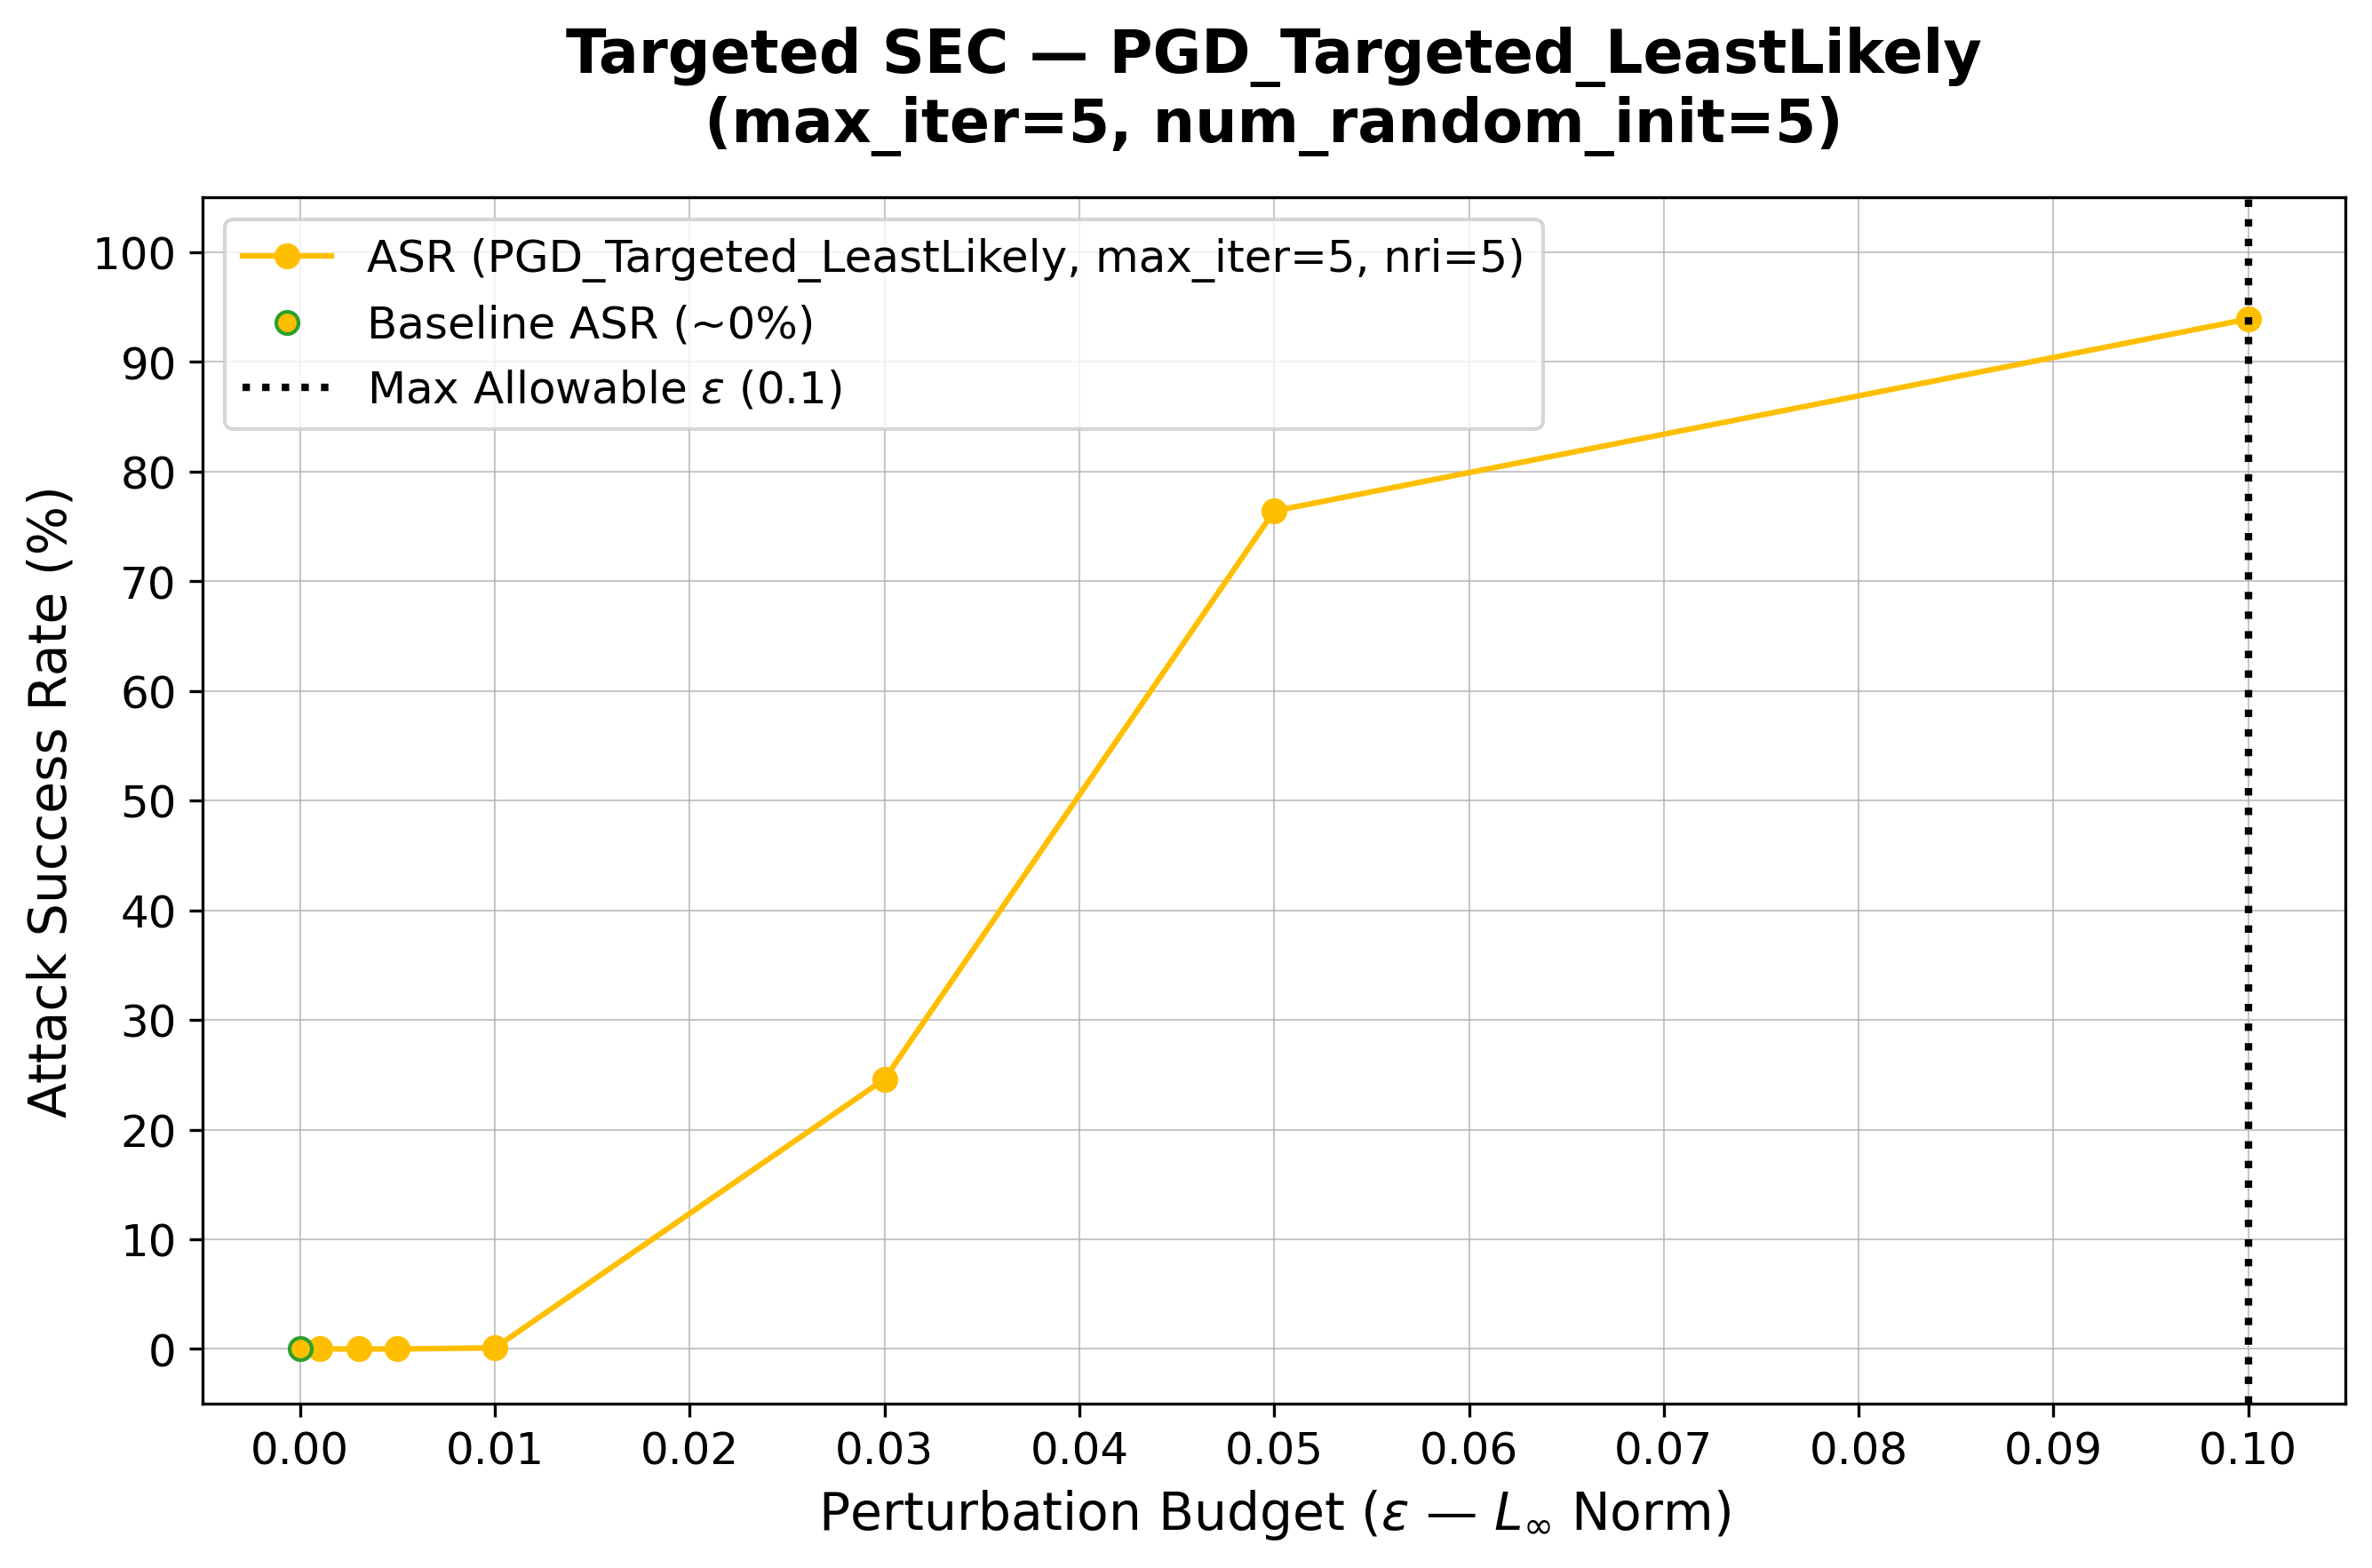
\includegraphics[width=\textwidth]{PGD_Error_specific/LL/PGD_Targeted_LeastLikely_nri5_iter5_SEC.png}
        \caption{\texttt{max_iter} = 5}
        \label{fig:PGD_LL_nri5_iter5}
    \end{subfigure}

    \vspace{1em} % Spazio verticale tra le righe di immagini
    % Sotto-figura 3
    \begin{subfigure}[b]{0.45\textwidth}
        \centering
        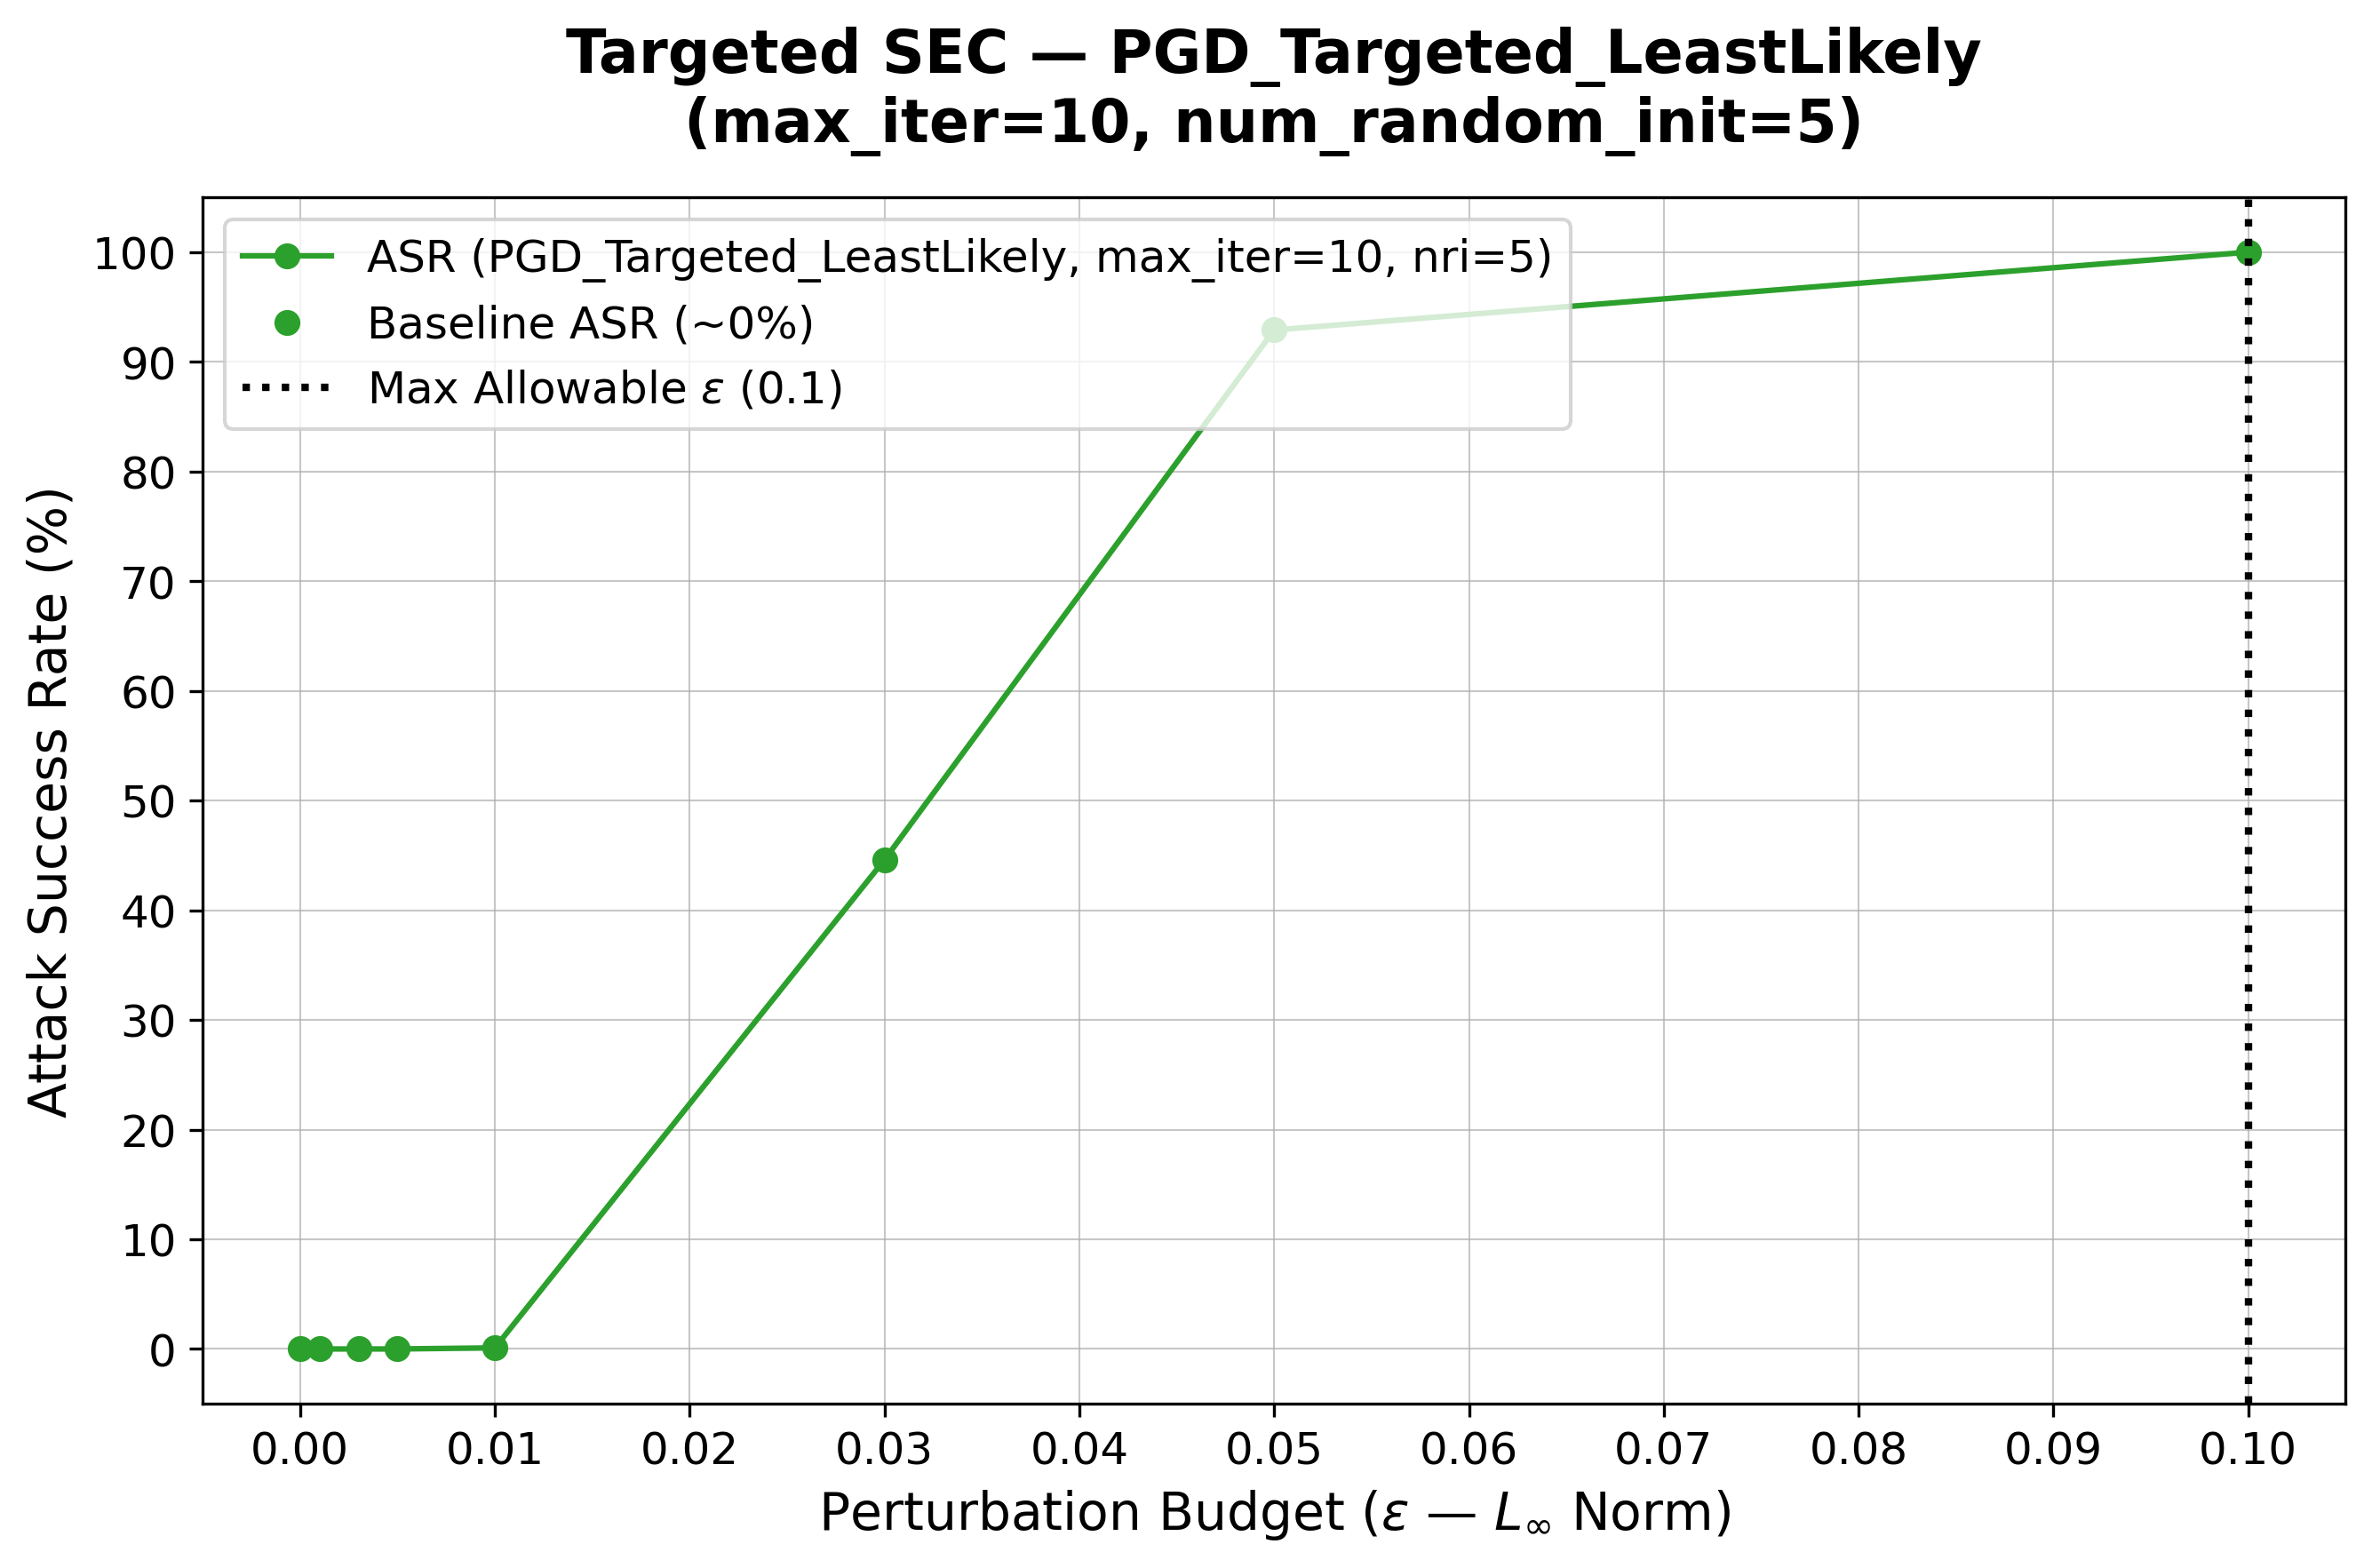
\includegraphics[width=\textwidth]{PGD_Error_specific/LL/PGD_Targeted_LeastLikely_nri5_iter10_SEC.png}
        \caption{\texttt{max_iter} = 10}
        \label{fig:PGD_LL_nri5_iter10}
    \end{subfigure}
    \hfill
    % Sotto-figura 4
    \begin{subfigure}[b]{0.45\textwidth}
        \centering
        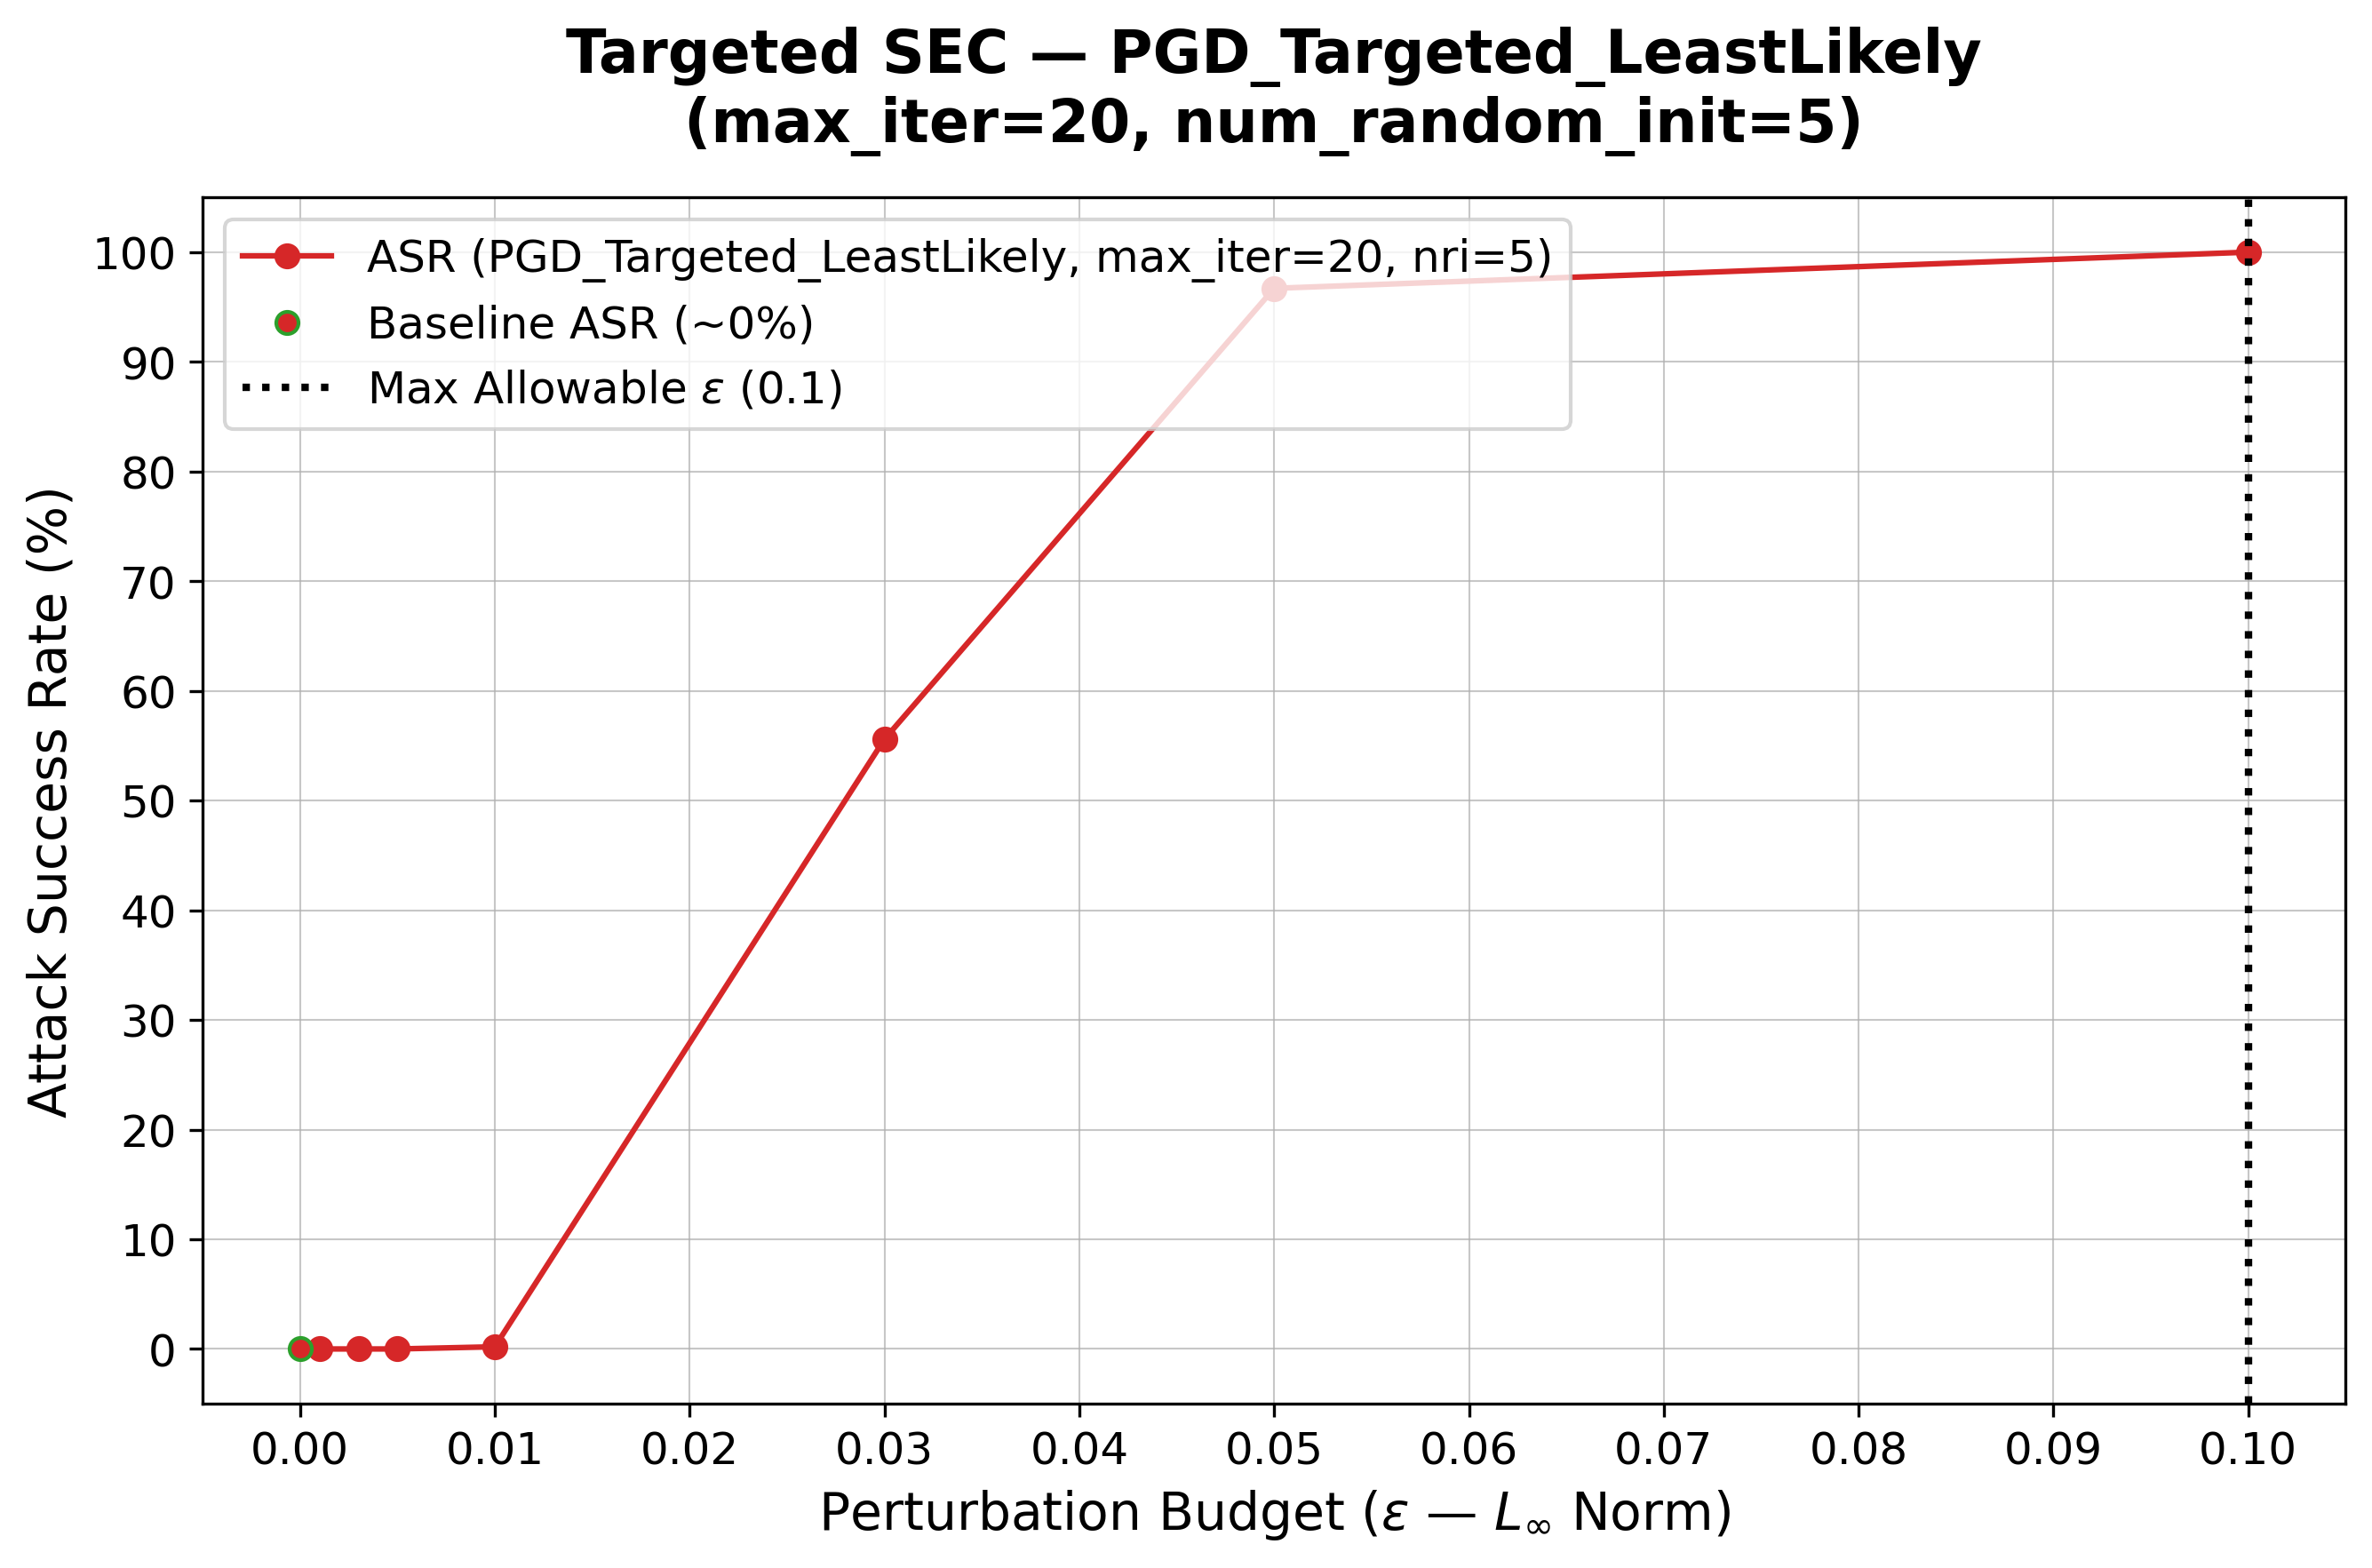
\includegraphics[width=\textwidth]{PGD_Error_specific/LL/PGD_Targeted_LeastLikely_nri5_iter20_SEC.png}
        \caption{\texttt{max_iter} = 20}
        \label{fig:PGD_LL_nri5_iter20}
    \end{subfigure}
    \vspace{1em} % Spazio verticale tra le righe di immagini
    % Sotto-figura 5
    \begin{subfigure}[b]{0.45\textwidth}
        \centering
        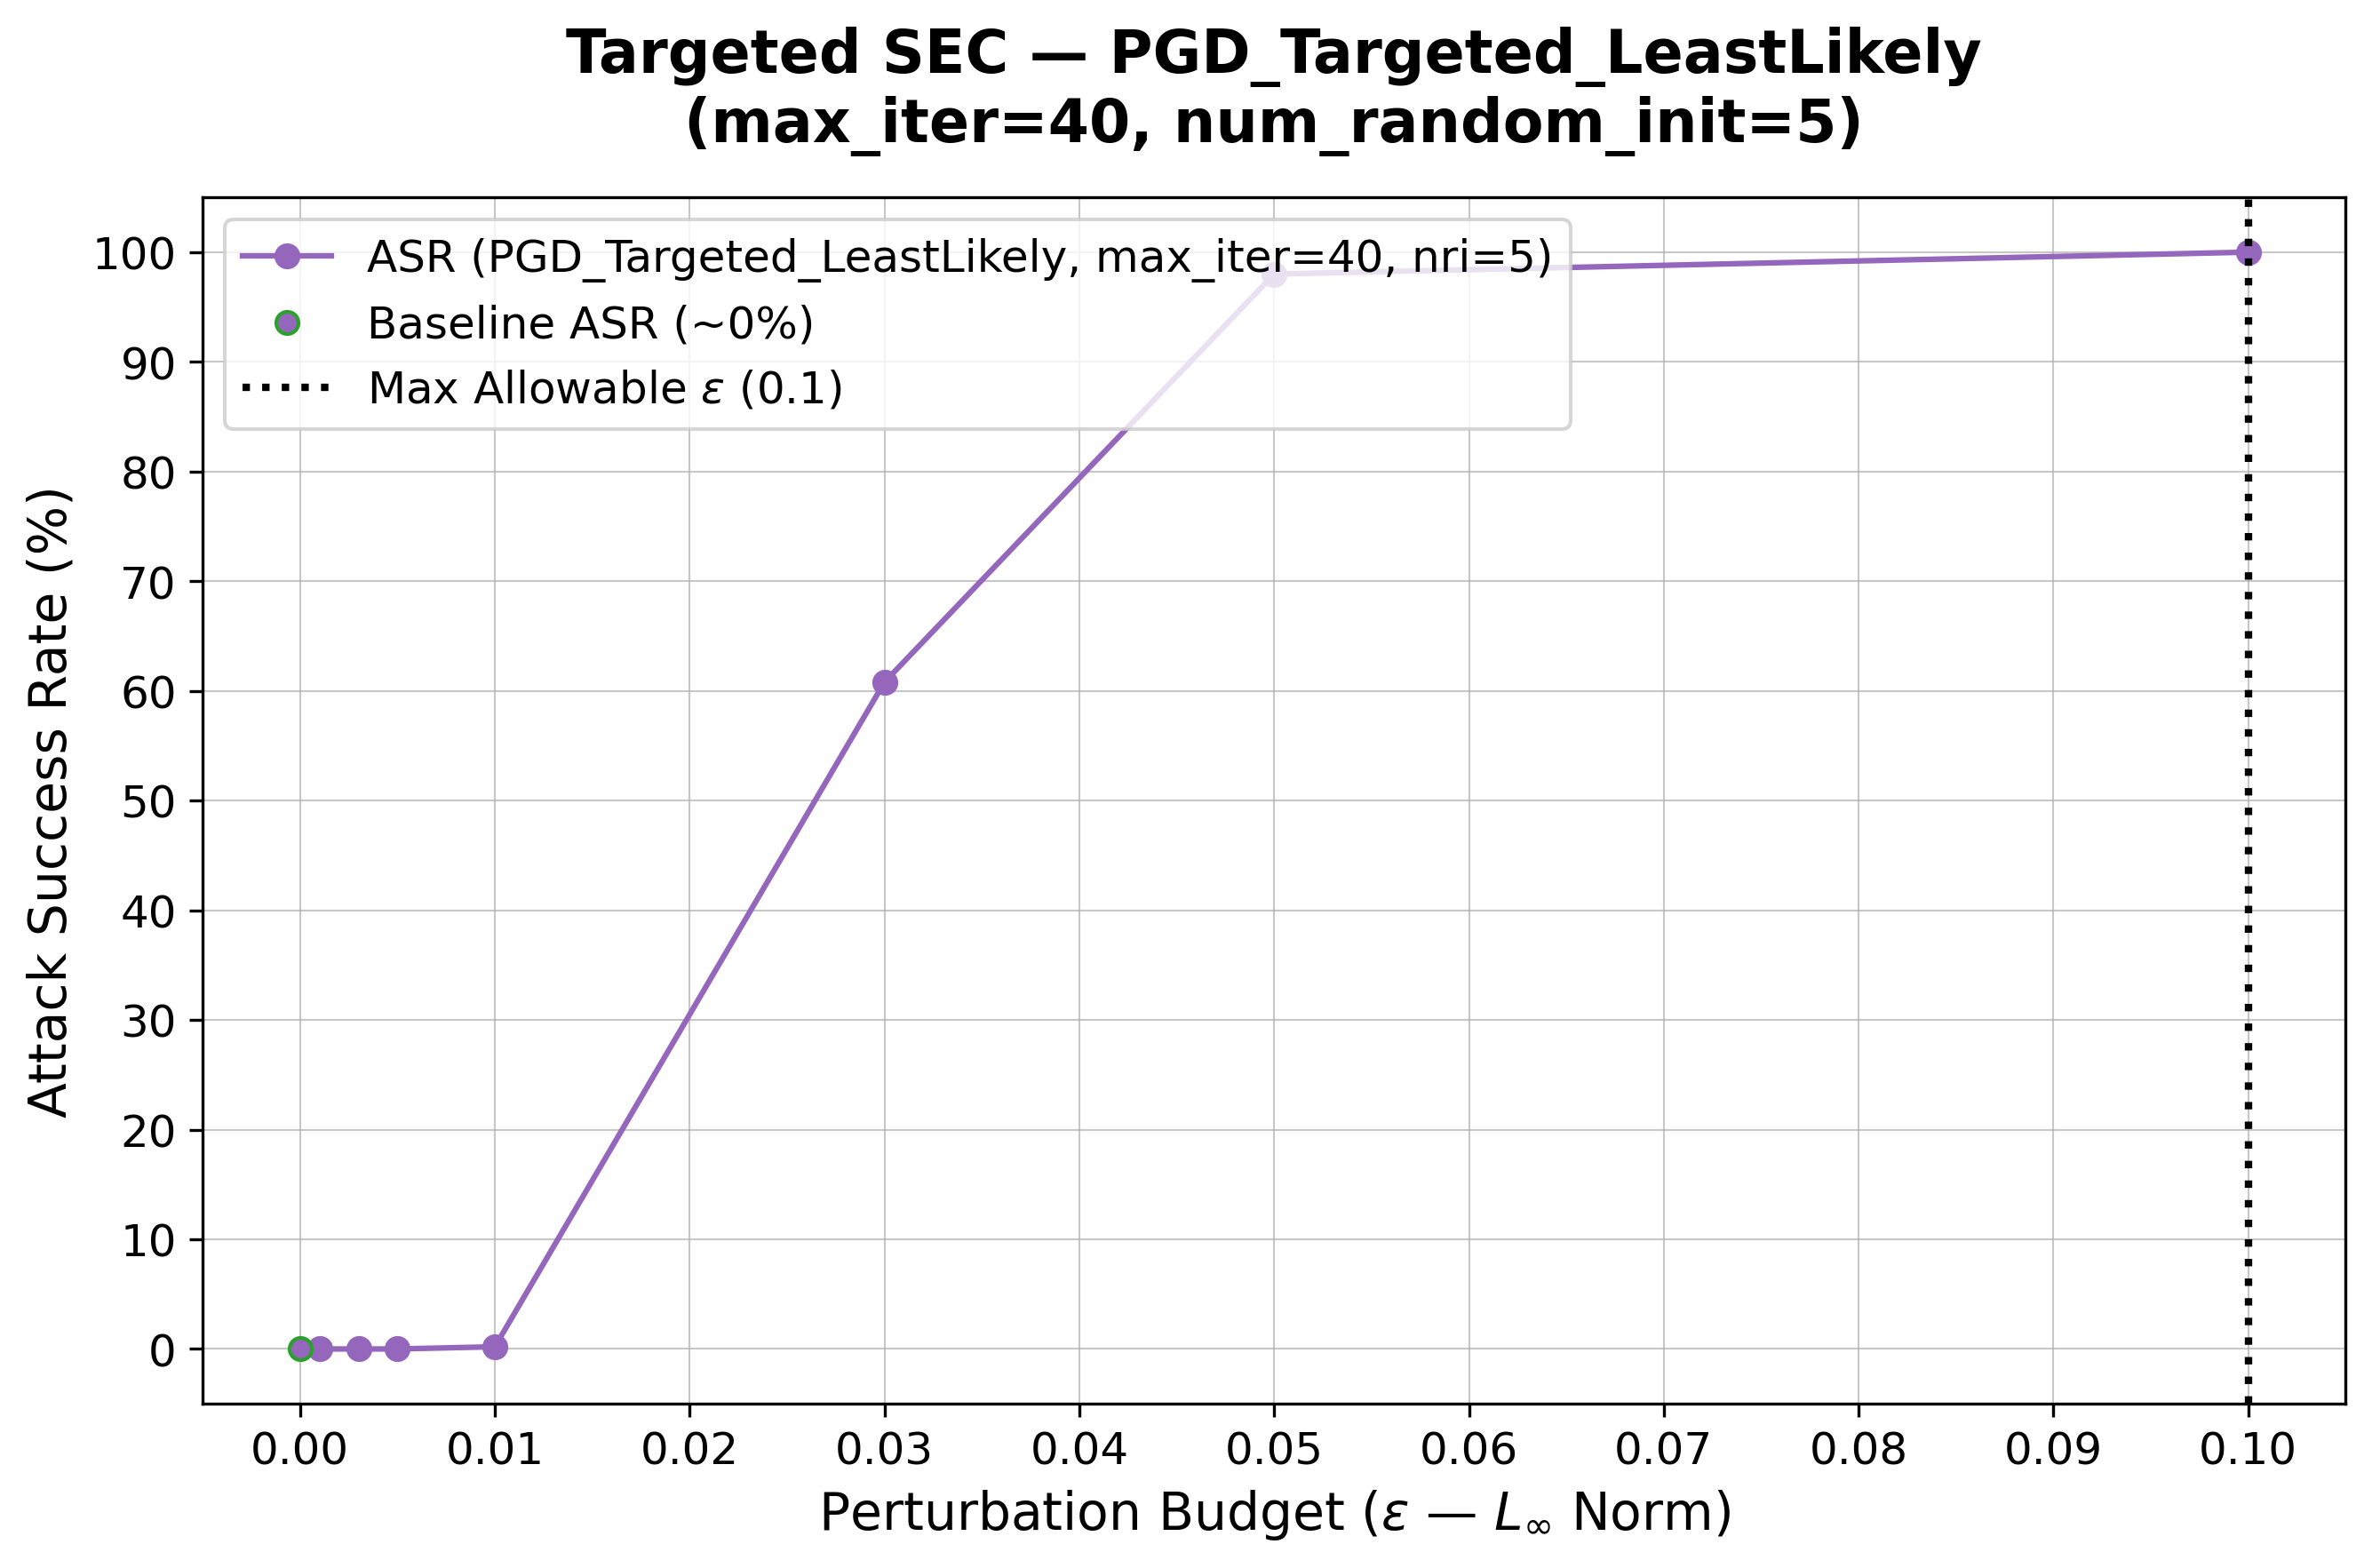
\includegraphics[width=\textwidth]{PGD_Error_specific/LL/PGD_Targeted_LeastLikely_nri5_iter40_SEC.png}
        \caption{\texttt{max_iter} = 40}
        \label{fig:PGD_LL_nri5_iter40}
    \end{subfigure}
    \caption{PGD Least Likely - Iterazioni a confronto per \texttt{nri} = 5}
    \label{fig:PGD_LL_iterations_nri5}
\end{figure}

% -- GRAFICO COMPARATIVO PER VARI NRI E MAX ITER--
\begin{figure}[H]
    \centering
    
    % Il \makebox centrato sulla larghezza del testo garantisce la simmetria perfetta
    \makebox[\textwidth][c]{
        \begin{tabular}{cc}
            
            % Sotto-figura 1 (Sinistra, Riga 1)
            \begin{subfigure}[b]{0.55\textwidth}
                \centering
                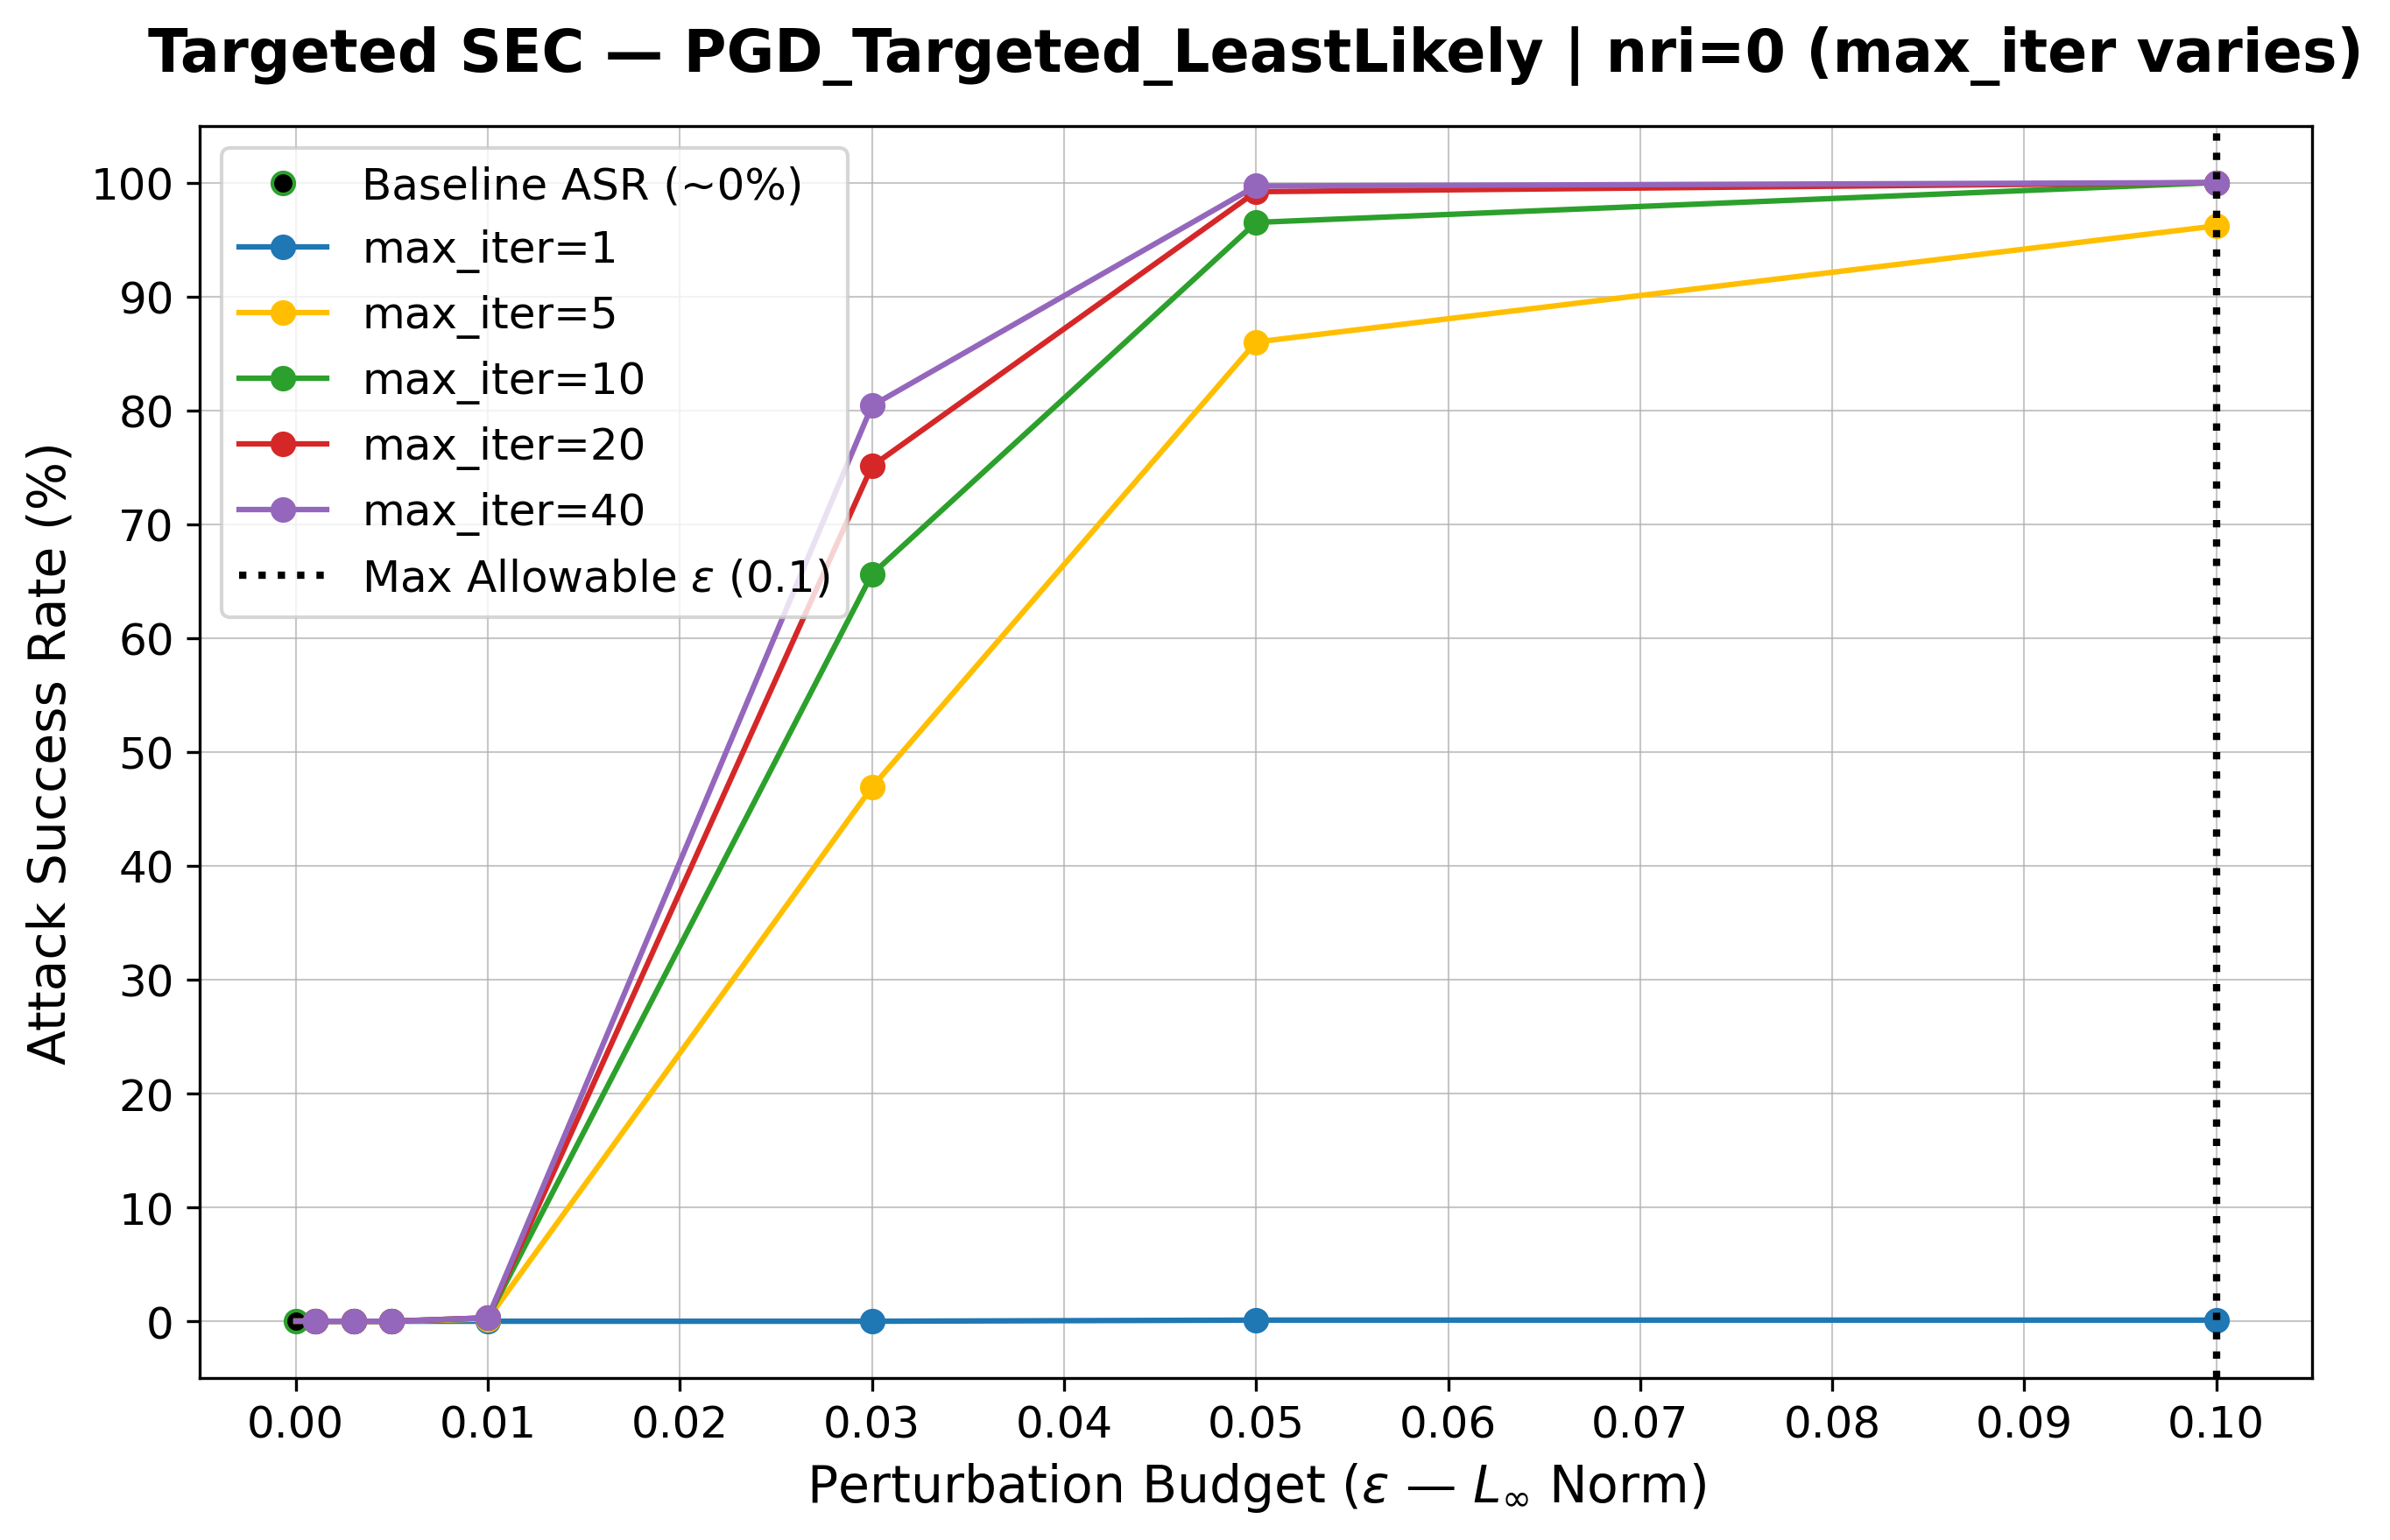
\includegraphics[width=\textwidth]{PGD_Error_specific/LL/PGD_Targeted_LeastLikely_nri0_comparative_maxiter_SEC.png}
                \caption{PGD Least Likely con \texttt{nri} = 0}
                \label{fig:PGD_LL_nri0_vari_iter}
            \end{subfigure}
            &
            % Sotto-figura 2 (Destra, Riga 1)
            \begin{subfigure}[b]{0.55\textwidth}
                \centering
                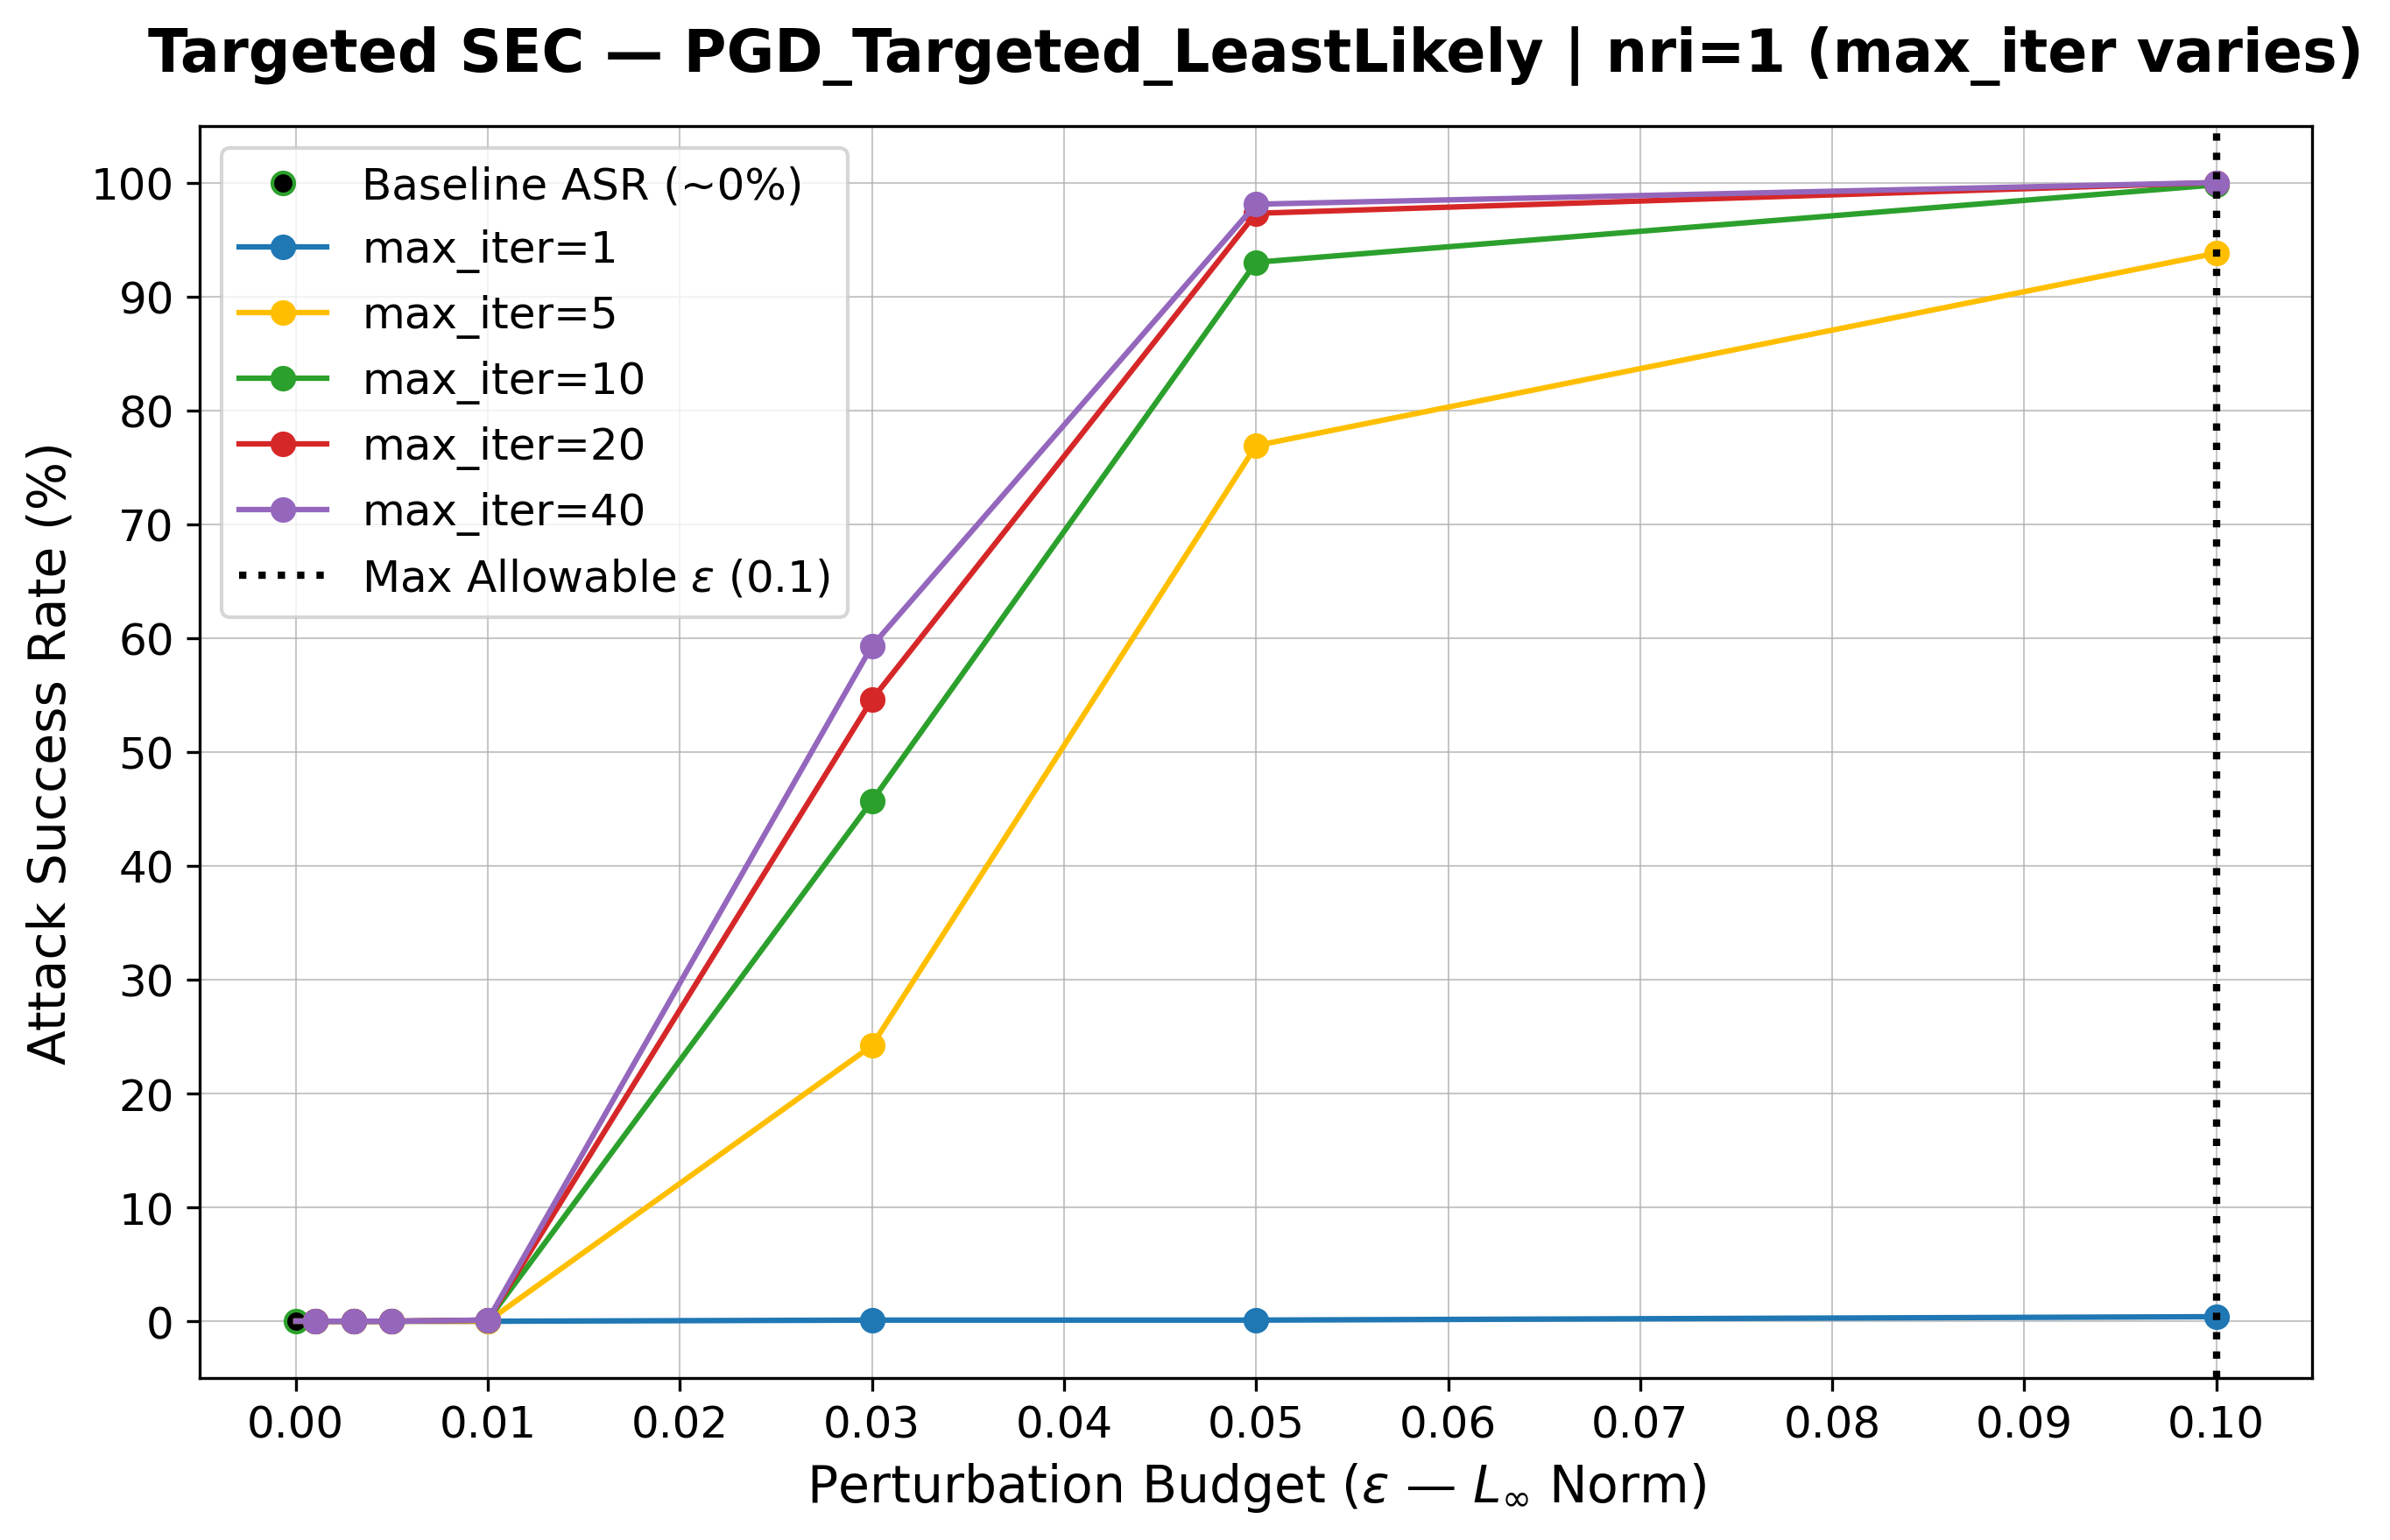
\includegraphics[width=\textwidth]{PGD_Error_specific/LL/PGD_Targeted_LeastLikely_nri1_comparative_maxiter_SEC.png}
                \caption{PGD Least Likely con \texttt{nri} = 1}
                \label{fig:PGD_LL_nri1_vari_iter}
            \end{subfigure} \\ [1em] % Spazio verticale tra le righe
            
            % Sotto-figura 3 (Sinistra, Riga 2)
            \begin{subfigure}[b]{0.55\textwidth}
                \centering
                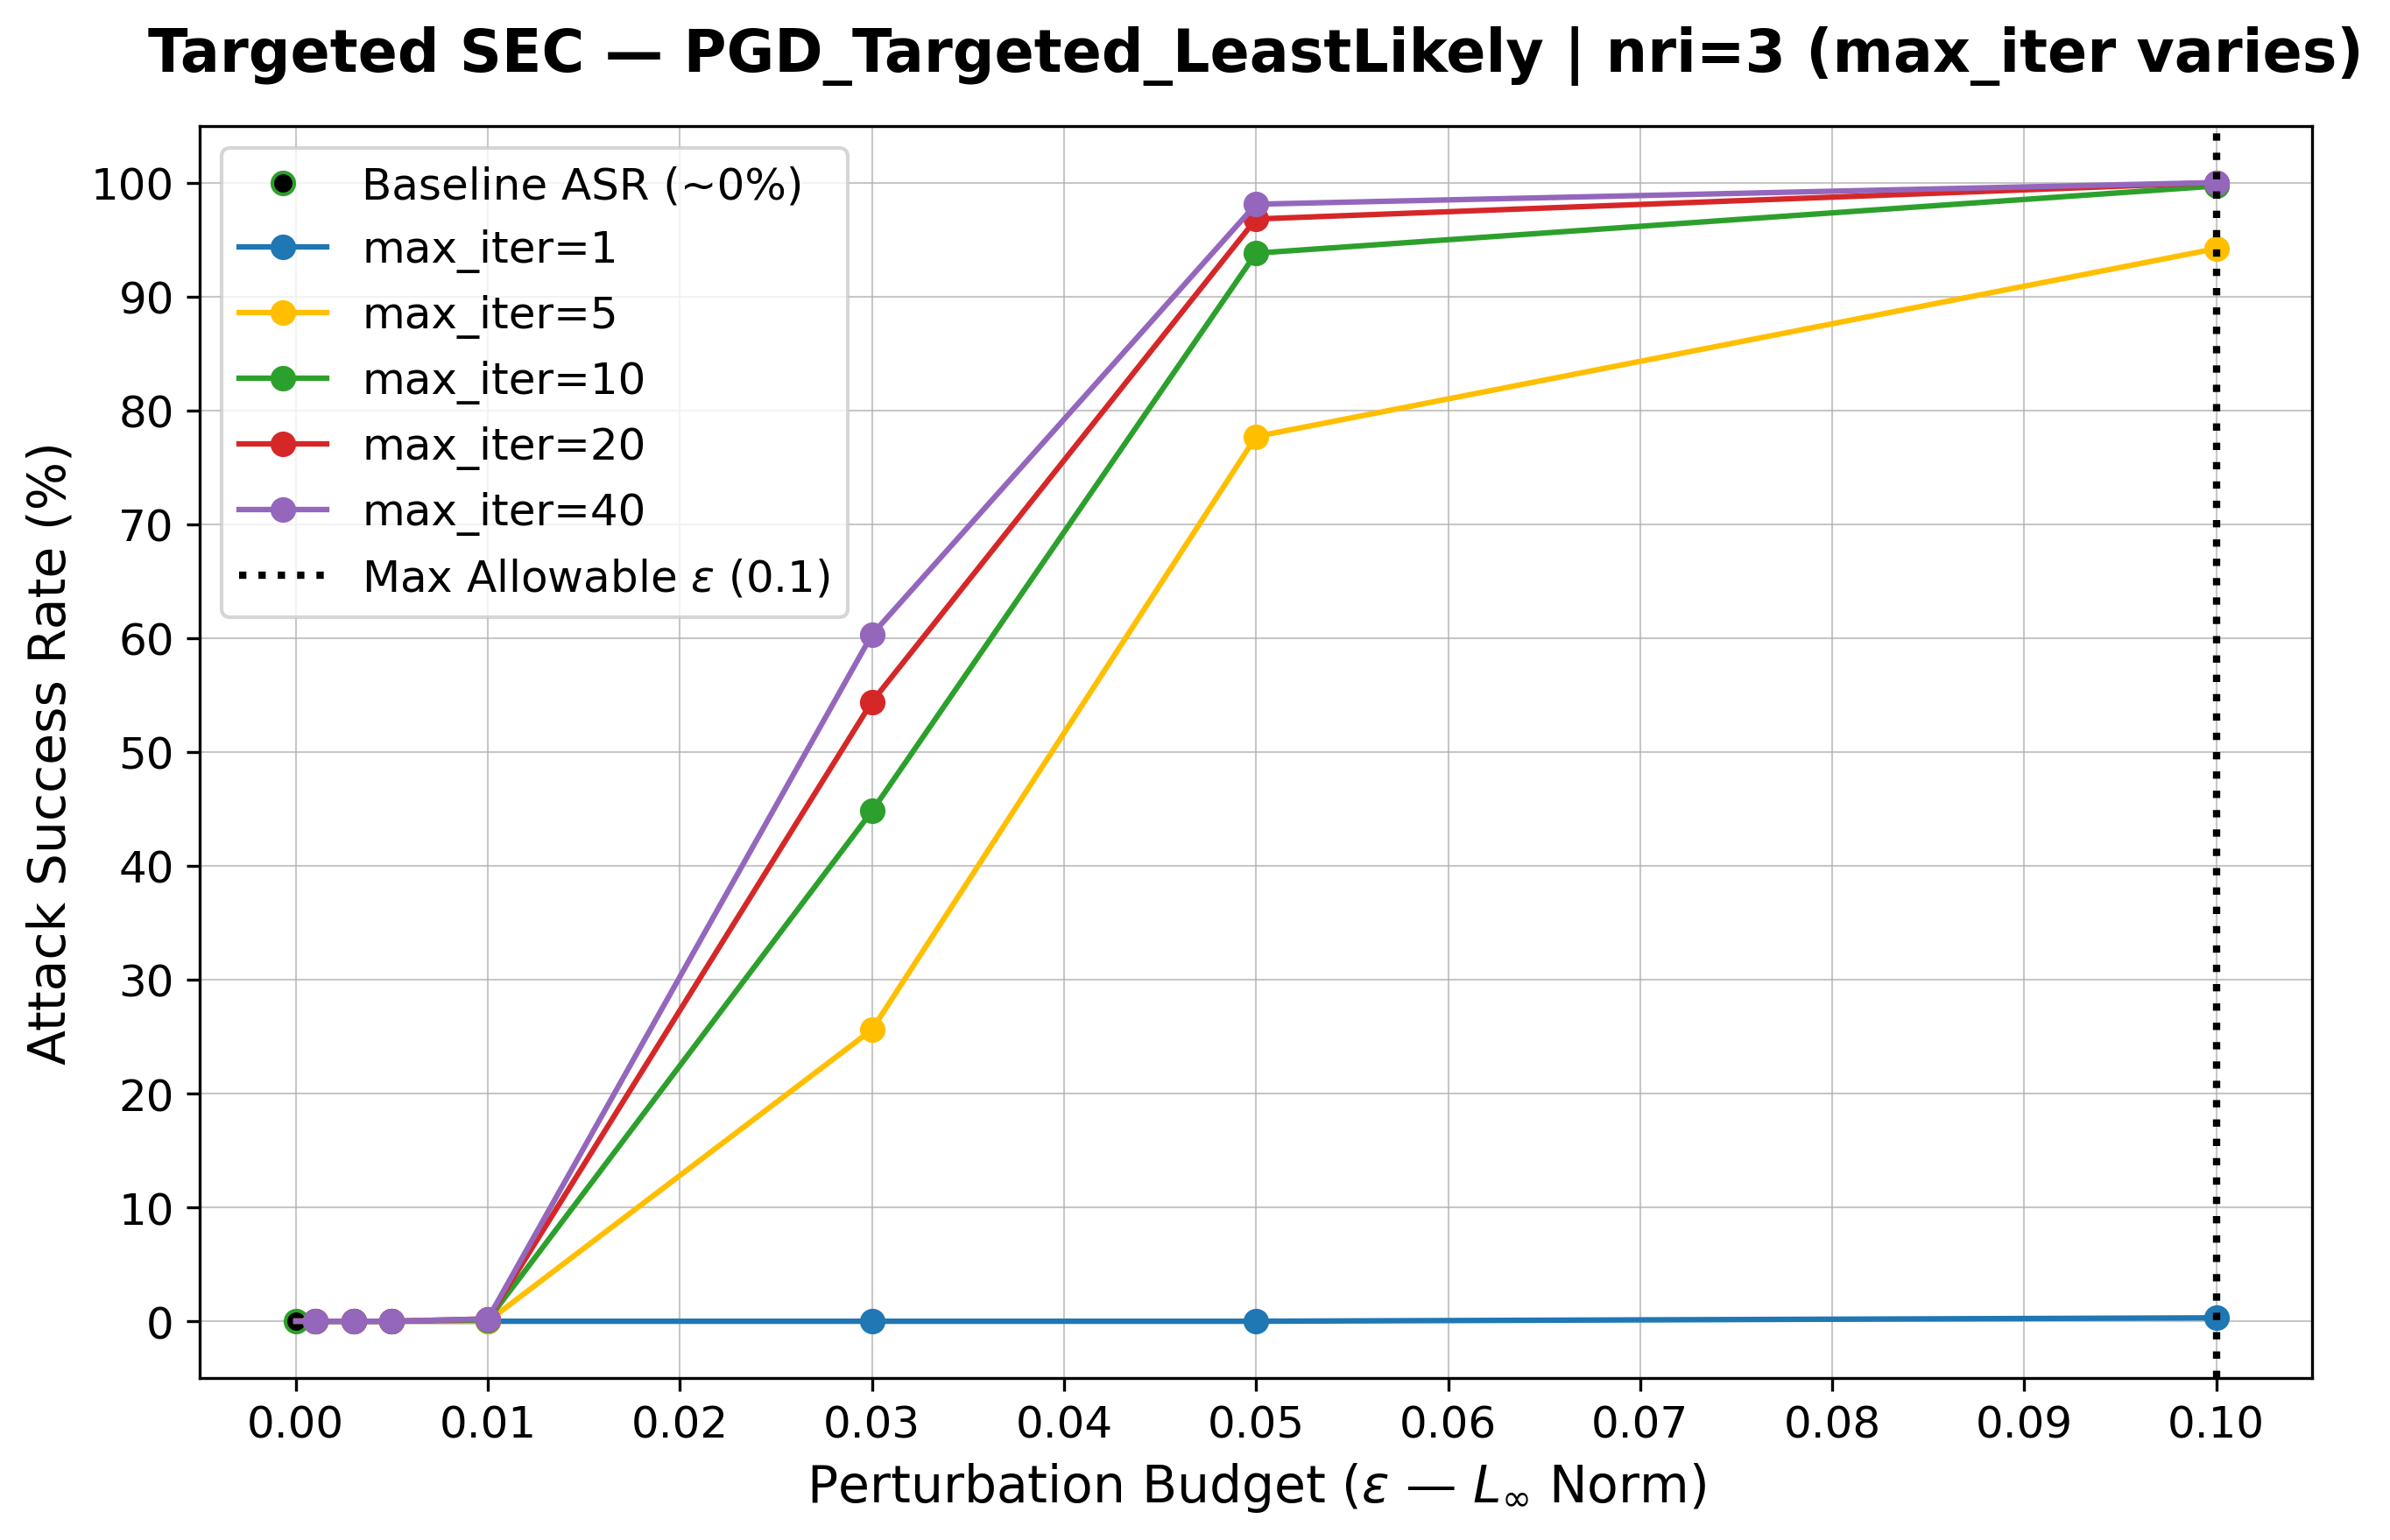
\includegraphics[width=\textwidth]{PGD_Error_specific/LL/PGD_Targeted_LeastLikely_nri3_comparative_maxiter_SEC.png}
                \caption{PGD Least Likely con \texttt{nri} = 3}
                \label{fig:PGD_LL_nri3_vari_iter}
            \end{subfigure}
            &
            % Sotto-figura 4 (Destra, Riga 2)
            \begin{subfigure}[b]{0.55\textwidth}
                \centering
                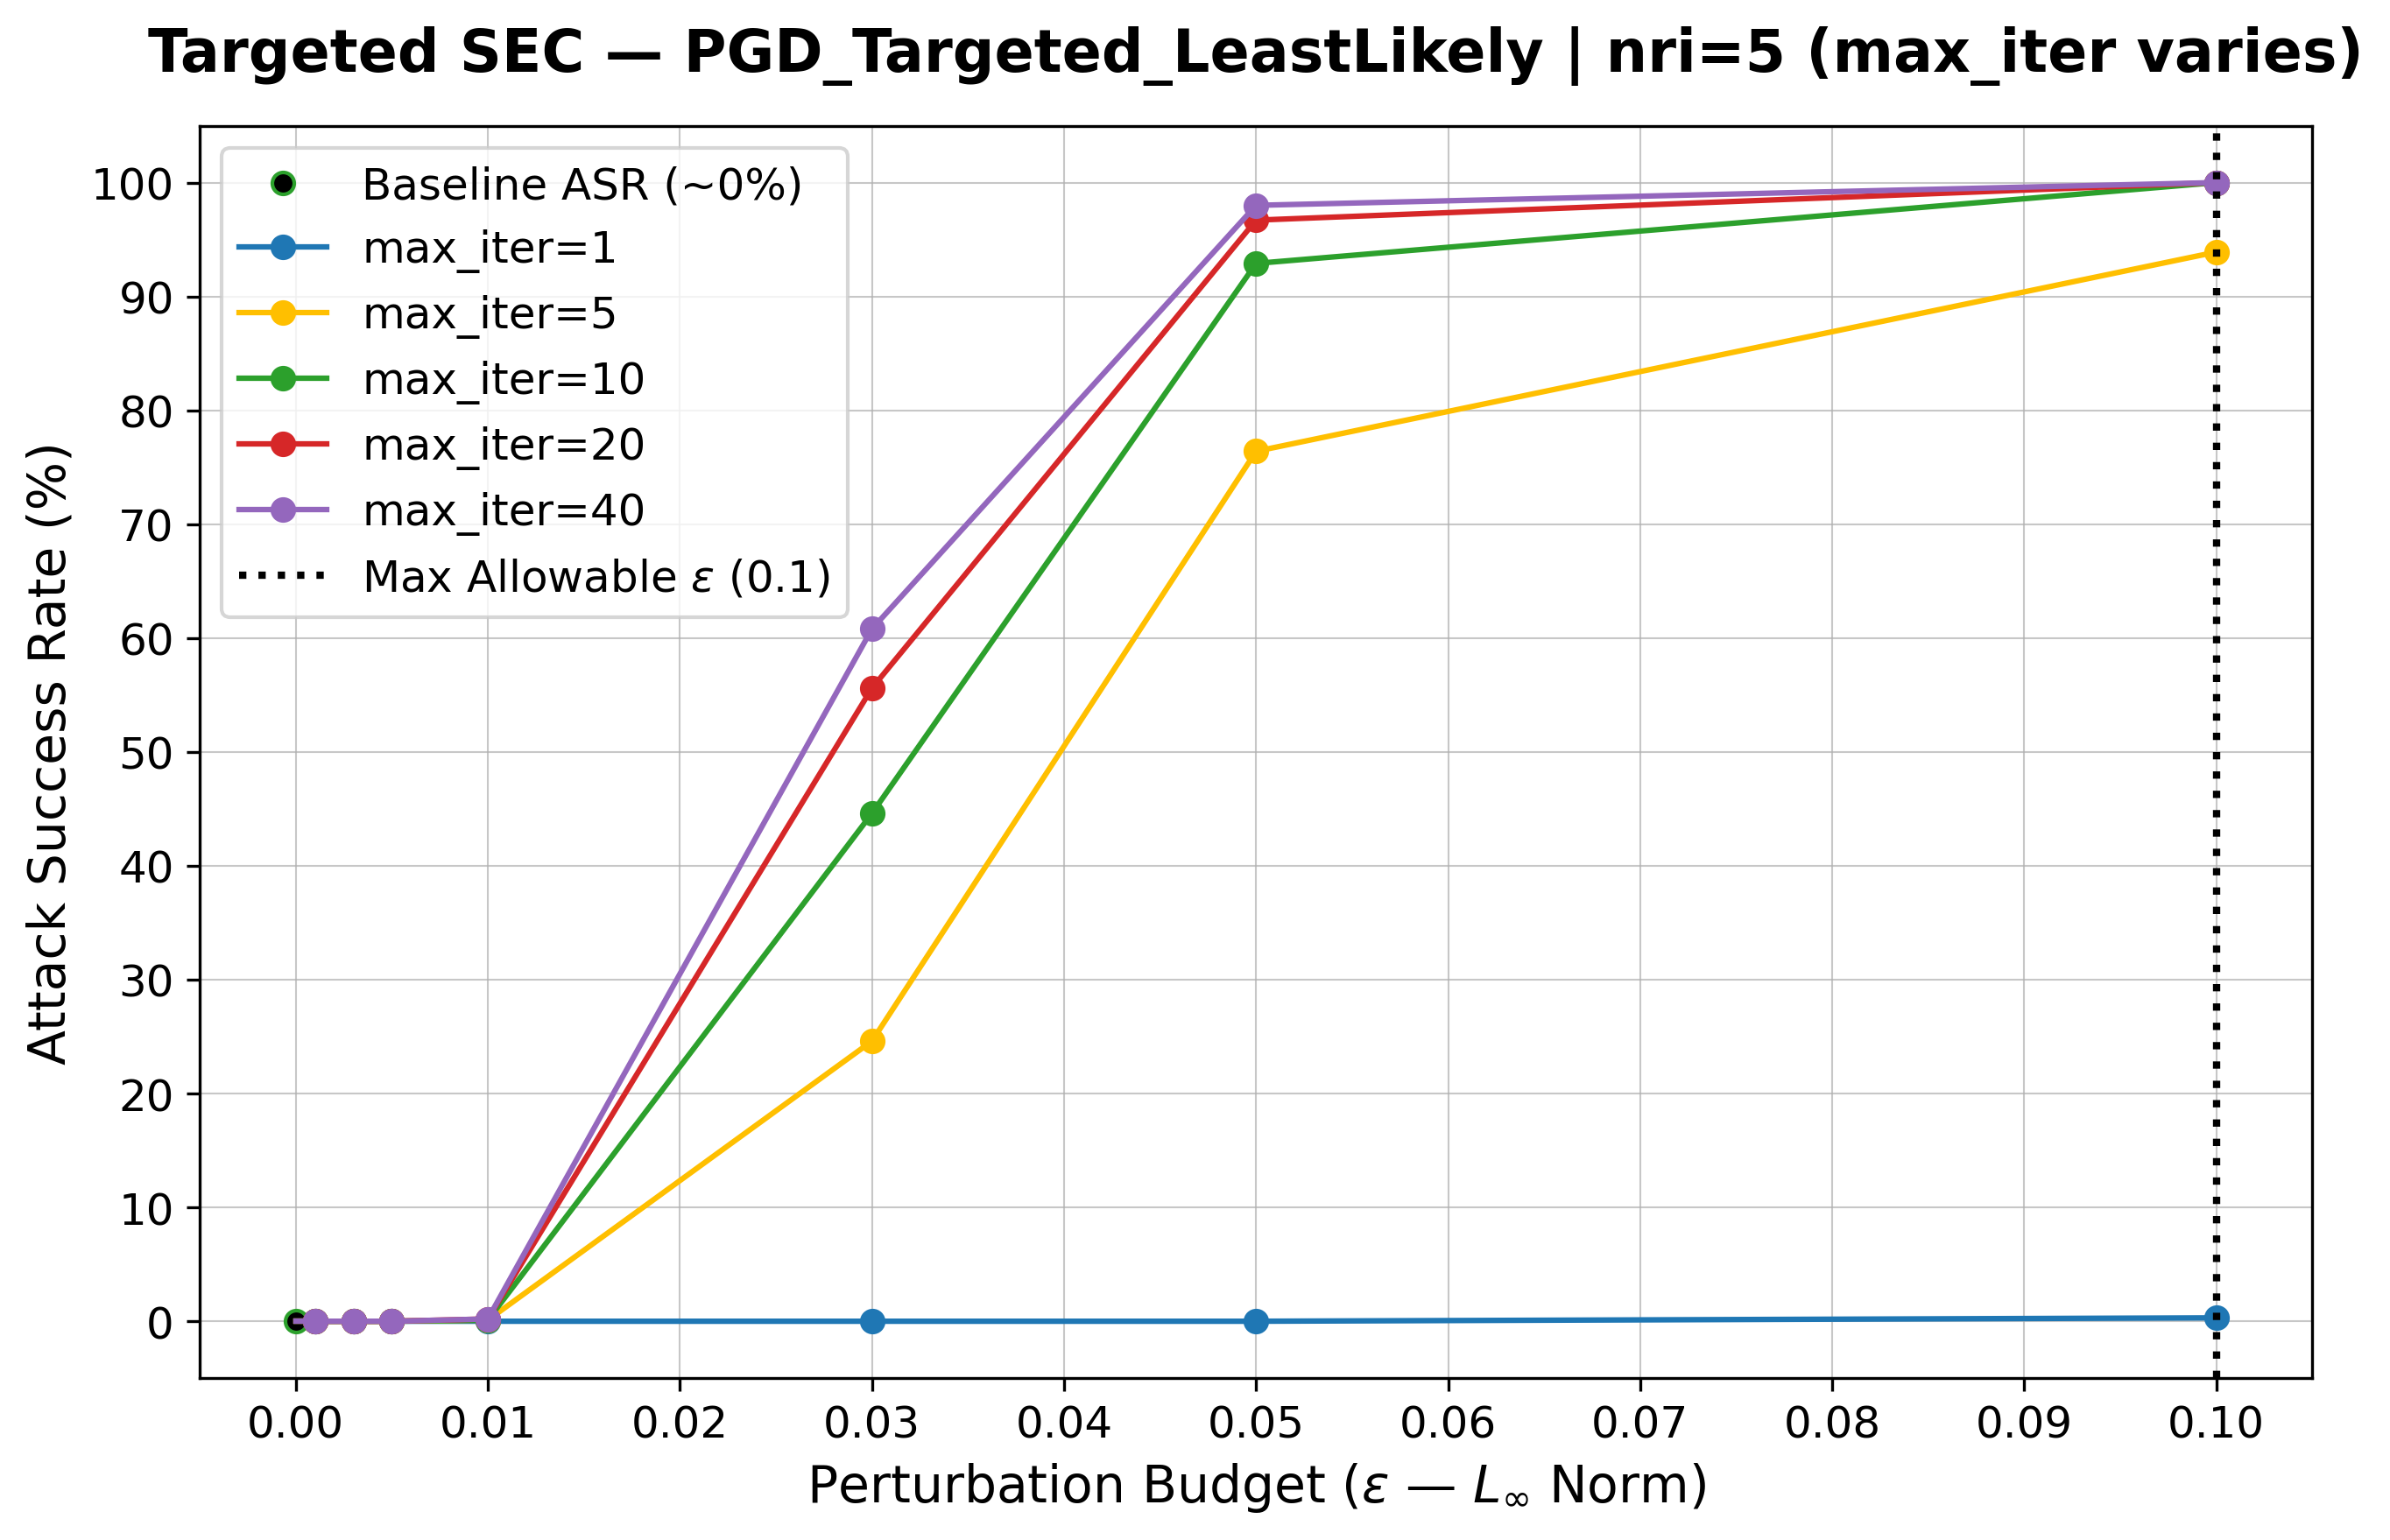
\includegraphics[width=\textwidth]{PGD_Error_specific/LL/PGD_Targeted_LeastLikely_nri5_comparative_maxiter_SEC.png}
                \caption{PGD Least Likely con \texttt{nri} = 5}
                \label{fig:PGD_LL_nri5_vari_iter}
            \end{subfigure}
            
        \end{tabular}
    }
    
    \caption{PGD Least Likely - Iterazioni a confronto per vari \texttt{nri}}
    \label{fig:PGD_LL_iterations_vari_nri}
\end{figure}

Anche in questo caso, la matrice di curve SEC evidenzia in modo inequivocabile l'assenza di benefici derivanti dall'introduzione di riavvii casuali. La configurazione deterministica (\texttt{nri} = 0) domina sistematicamente le varianti stocastiche, confermando che, per un attacco a bersaglio semanticamente remoto, la componente casuale non solo è superflua, ma addirittura controproducente.

Un ulteriore elemento di rilevanza che emerge dai dati, visibile nella matrice in Figura~\ref{fig:PGD_LL_iterations_vari_nri}, è il totale e sistematico fallimento dell'attacco quando configurato con \texttt{max\_iter} = 1, indipendentemente dal numero di inizializzazioni casuali (\texttt{num\_random\_init}) applicate. In tutti gli scenari testati, l'\textit{Attack Success Rate} per il target \textit{Least Likely} con una singola iterazione rimane rigorosamente ancorato allo~0\%.
Il dato scientificamente più interessante è che l'introduzione della stocasticità (\texttt{num\_random\_init} > 0) non mitiga in alcun modo questo risultato. Se l'algoritmo applica un salto casuale iniziale, ma dispone poi di un unico passo di calcolo del gradiente (\texttt{max\_iter} = 1) per rimettersi in rotta, la dinamica offensiva non cambia. Partire da un punto leggermente sfalsato all'interno del minuscolo \textit{budget} $\epsilon$ e tracciare una singola retta di massima pendenza produce inevitabilmente un risultato che non è in grado di raggiungere il target. L'immagine alterata finisce per cadere all'interno della regione di pertinenza di una delle innumerevoli classi limitrofe (causando un attacco di tipo \textit{error-generic} riuscito), ma manca totalmente la minuscola e lontana area di accettazione della classe \textit{Least Likely}.

\subsubsection{Carlini \& Wagner Attack}
L'algoritmo \textit{Carlini \& Wagner} (CW) chiude la disamina degli attacchi mirati proponendo un approccio diverso rispetto ai metodi basati sul gradiente proiettato. Come ampiamente discusso nelle sezioni relative a BIM e PGD, il limite strutturale degli attacchi \textit{budget-constrained} emerge quando la distanza semantica tra l'immagine originale e la classe bersaglio è estrema.

Essendo un CW un attacco ottimizzante, la sua formulazione matematica non prevede un vincolo esplicito sulla magnitudo della perturbazione.

L'algoritmo esplorerà lo spazio alla ricerca del percorso ottimale verso il target e, solo a posteriori, verrà misurato il rumore effettivamente speso. Per mantenere la coerenza scientifica con i test precedenti, è stata implementata una logica di filtraggio: se per raggiungere la classe bersaglio CW genera una perturbazione la cui norma $L_\infty$ supera la soglia limite prestabilita (\texttt{EPSILON\_LIMIT} = 0.1), l'immagine viene rigettata (considerata fuori budget) e non concorre ad accrescere l'\textit{Attack Success Rate} (ASR).

Considerato l'ingente costo computazionale dell'ottimizzatore, i test sono stati eseguiti sul \texttt{dataset\_1\_per\_person} (100 immagini). La modalità di attacco è stata limitata al solo scenario \textit{Fixed}, sempre per una questione di costo computazionale dell'algoritmo e anche per gli scarsi risultati ottenuti nella modalità più semplice.

La griglia di esplorazione iper-parametrica ha incrociato la profondità dell'ottimizzatore (\texttt{max\_iter} $\in \{1, 20, 50\}$) e il passo di discesa (\texttt{learning\_rate} $\in \{0.01, 0.1\}$), valutando per ogni combinazione la percentuale di attacchi mirati andati a buon fine.

\begin{verbatim}
    MAX_ITER_LIST      = [1, 20, 50]
    LEARNING_RATE_LIST = [0.01, 0.1]
    CONFIDENCE_LIST    = [0.0]
\end{verbatim}


\subsubsection*{Fixed Attack}
L'analisi empirica dell'attacco Carlini \& Wagner (CW) in modalità \textit{Fixed} restituisce un risultato inaspettato: l'algoritmo fallisce totalmente l'obiettivo. Come si evince dai dati raccolti in tabella~\ref{tab:cw_targeted_fixed_results} e dalla \textit{SEC} piatta (figura~\ref{fig:sec_fixed_cw}), per l'intero spettro di iperparametri testati (\texttt{max\_iter} fino a 50 e \texttt{learning\_rate} fino a 0.1), l'\textit{Attack Success Rate} (ASR) si attesta rigorosamente allo 0.0\%. Su 100 immagini testate, nessuna è stata classificata nella classe bersaglio (ID 2026).

Per comprendere la natura di questo fallimento, è fondamentale analizzare la metrica del rumore medio (\texttt{mean\_linf\_raw}). I dati rivelano che le perturbazioni generate non hanno mai infranto il \textit{budget} tollerato: con un \texttt{learning\_rate} di 0.1, l'attacco si è arrestato a un'ampiezza massima di perturbazione pari a $0.0485$, ben al di sotto del limite rigido $\epsilon \le 0.1$. Ciò dimostra che CW non ha fallito perché "murato" dal vincolo spaziale (come avveniva per PGD nei target remoti), bensì perché l'ottimizzatore non ha avuto a disposizione un numero sufficiente di iterazioni per colmare la distanza necessaria.

L'algoritmo CW si affida all'ottimizzatore \textit{Adam} per minimizzare la complessa funzione obiettivo. A differenza di BIM, che sfrutta l'operatore \textit{sign()} per compiere sbalzi aggressivi e massimali a ogni step, CW modula la discesa in modo più conservativo. Di conseguenza, il team ipotizza che 50 iterazioni sono troppo poche per consentire ad \textit{Adam} di far convergere l'immagine verso il target. 

A sostegno di questa ipotesi, il limite empirico legato al costo computazionale trova pieno riscontro nel paper ufficiale rilasciato da Carlini e Wagner \cite{carlini2017towards}. Come dimostrato nello studio, l'algoritmo CW è matematicamente concepito per forzare l'inganno in modalità mirata con tassi di successo del 100\%, generando perturbazioni quasi impercettibili. Tuttavia, tale efficacia è ottenibile solo con un numero elevato di iterazioni. Nel dettaglio, il fallimento dell'algoritmo nel presente setup è matematicamente coerente con il comportamento atteso descritto dagli autori per tre ragioni strutturali:

\begin{enumerate}
    \item \textbf{Carico iterativo di base:} Nella Sezione V.C (pag. 8), gli autori specificano di eseguire ben 10.000 iterazioni di discesa del gradiente con \textit{Adam} per ogni singolo step di ricerca \cite{carlini2017towards}. Inoltre, viene evidenziato che l'ottimizzatore necessita empiricamente di almeno 1.000 iterazioni per raggiungere il 95\% dell'ottimo di convergenza (pag. 8, nota a piè di pagina 9) \cite{carlini2017towards}.
    
    \item \textbf{Ricerca del parametro \textit{c}:} L'algoritmo originale non esegue una singola passata, ma un processo di ricerca binaria (\textit{binary search}) per calibrare il parametro $c$, essenziale per bilanciare la distanza della perturbazione e il successo dell'attacco. Carlini e Wagner dichiarano di eseguire 20 iterazioni di ricerca binaria (Sez. V.C, pag. 8), ripetendo le 10.000 iterazioni di \textit{gradient descent} per ognuna di esse \cite{carlini2017towards}.
    
    \item \textbf{Criticità e oscillazioni della metrica $\boldsymbol{L_{\infty}}$:} La scelta della distanza $L_{\infty}$ inasprisce ulteriormente il limite computazionale. Come analizzato nella Sezione VI.C (pag. 10), la metrica $L_{\infty}$ non è completamente differenziabile e la discesa del gradiente standard tende a bloccarsi "oscillando tra due soluzioni sub-ottimali" \cite{carlini2017towards}. Per mitigare il problema, l'algoritmo impiega una penalità iterativa decrescente basata su una soglia $\tau$, che viene ridotta di un fattore $0.9$ a ogni ciclo di successo \cite{carlini2017towards}. Questo raffinamento iterativo necessita di tempi fisiologici lunghissimi per stabilizzarsi, rendendo impossibile superare l'oscillazione iniziale in appena 50 iterazioni complessive.
\end{enumerate}

In conclusione, l'ASR dello 0.0\% registrato per CW $L_{\infty}$ non costituisce un'anomalia di implementazione, ma bensì una dimostrazione empirica di come sia impossibile ottenere risultati soddisfacenti con un numero limitato di iterazioni.

Questo limite teorico si scontra drammaticamente con il vincolo applicativo del tempo di esecuzione. Dai log emerge che l'elaborazione di 100 immagini per 50 iterazioni ha richiesto oltre 18.400 secondi (circa 5.1 ore). Concedere a CW le centinaia o migliaia di iterazioni per eludere un bersaglio specifico comporterebbe tempi di esecuzione proibitivi per il contesto del nostro progetto.

\begin{table}[h]
    \centering
    \begin{tabular}{cccccc}
        \toprule
        \textbf{Max Iter} & \textbf{Learning Rate} & \textbf{ASR (\%)} & \textbf{Successi / Totali} & \textbf{Mean $L_\infty$} & \textbf{Tempo (s)} \\
        \midrule
        1  & 0.01 & 0.0 & 0 / 100 & 0.0050 & 918.25 \\
        1  & 0.10 & 0.0 & 0 / 100 & 0.0485 & 874.56 \\
        20 & 0.01 & 0.0 & 0 / 100 & 0.0050 & 9459.87 \\
        20 & 0.10 & 0.0 & 0 / 100 & 0.0485 & 5849.32 \\
        50 & 0.01 & 0.0 & 0 / 100 & 0.0050 & 17158.36 \\
        50 & 0.10 & 0.0 & 0 / 100 & 0.0485 & 18405.26 \\
        \bottomrule
    \end{tabular}
    \caption{Risultati dell'attacco CW Targeted (Fixed) al variare del numero massimo di iterazioni e del learning rate. La \textit{Confidence} è impostata a 0.0 per tutti i test.}
    \label{tab:cw_targeted_fixed_results}
\end{table}

\begin{figure}[H]
    \centering
    
    % Blocchiamo la struttura al centro della pagina sfruttando tutto lo spazio
    \makebox[\textwidth][c]{
        \begin{tabular}{cc}
            
            % Sotto-figura 1 (In alto a sinistra)
            \begin{subfigure}[b]{0.55\textwidth}
                \centering
                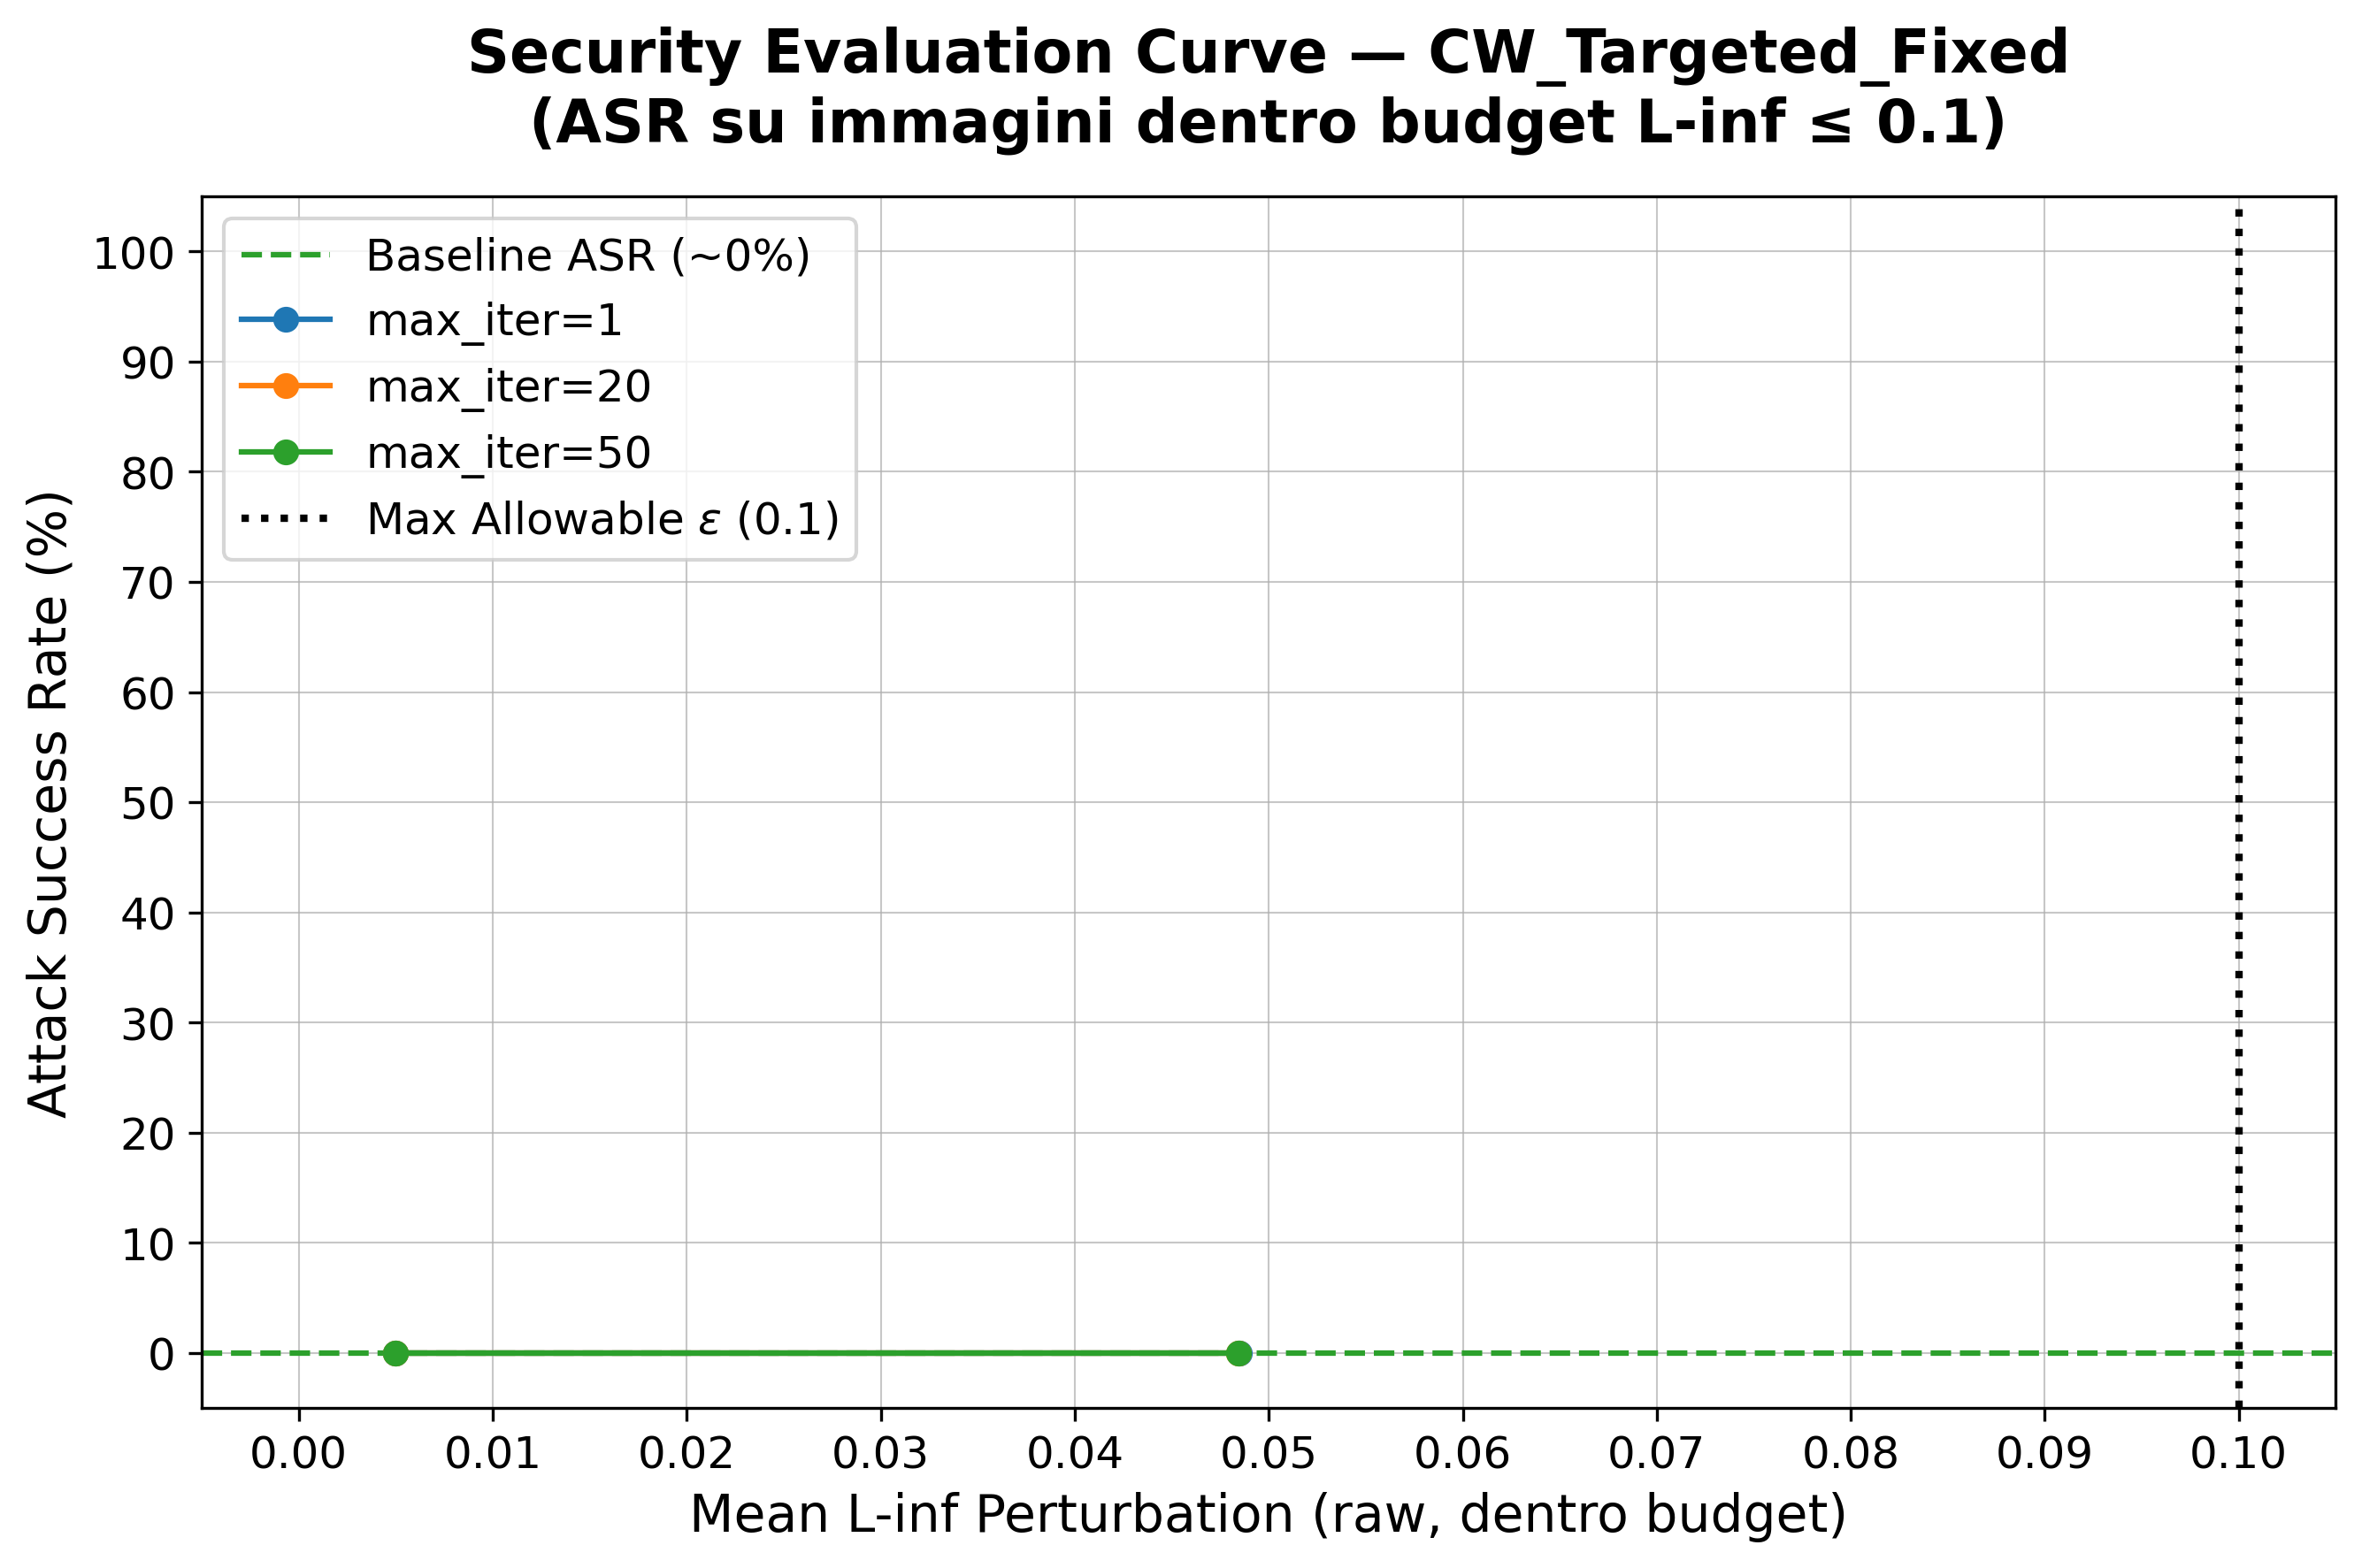
\includegraphics[width=\textwidth]{CW_Targeted/CW_Targeted_Fixed_SEC.png}
                \caption{SEC Generale}
                \label{fig:sec_fixed_cw}
            \end{subfigure}
            &
            % Sotto-figura 2 (In alto a destra)
            \begin{subfigure}[b]{0.55\textwidth}
                \centering
                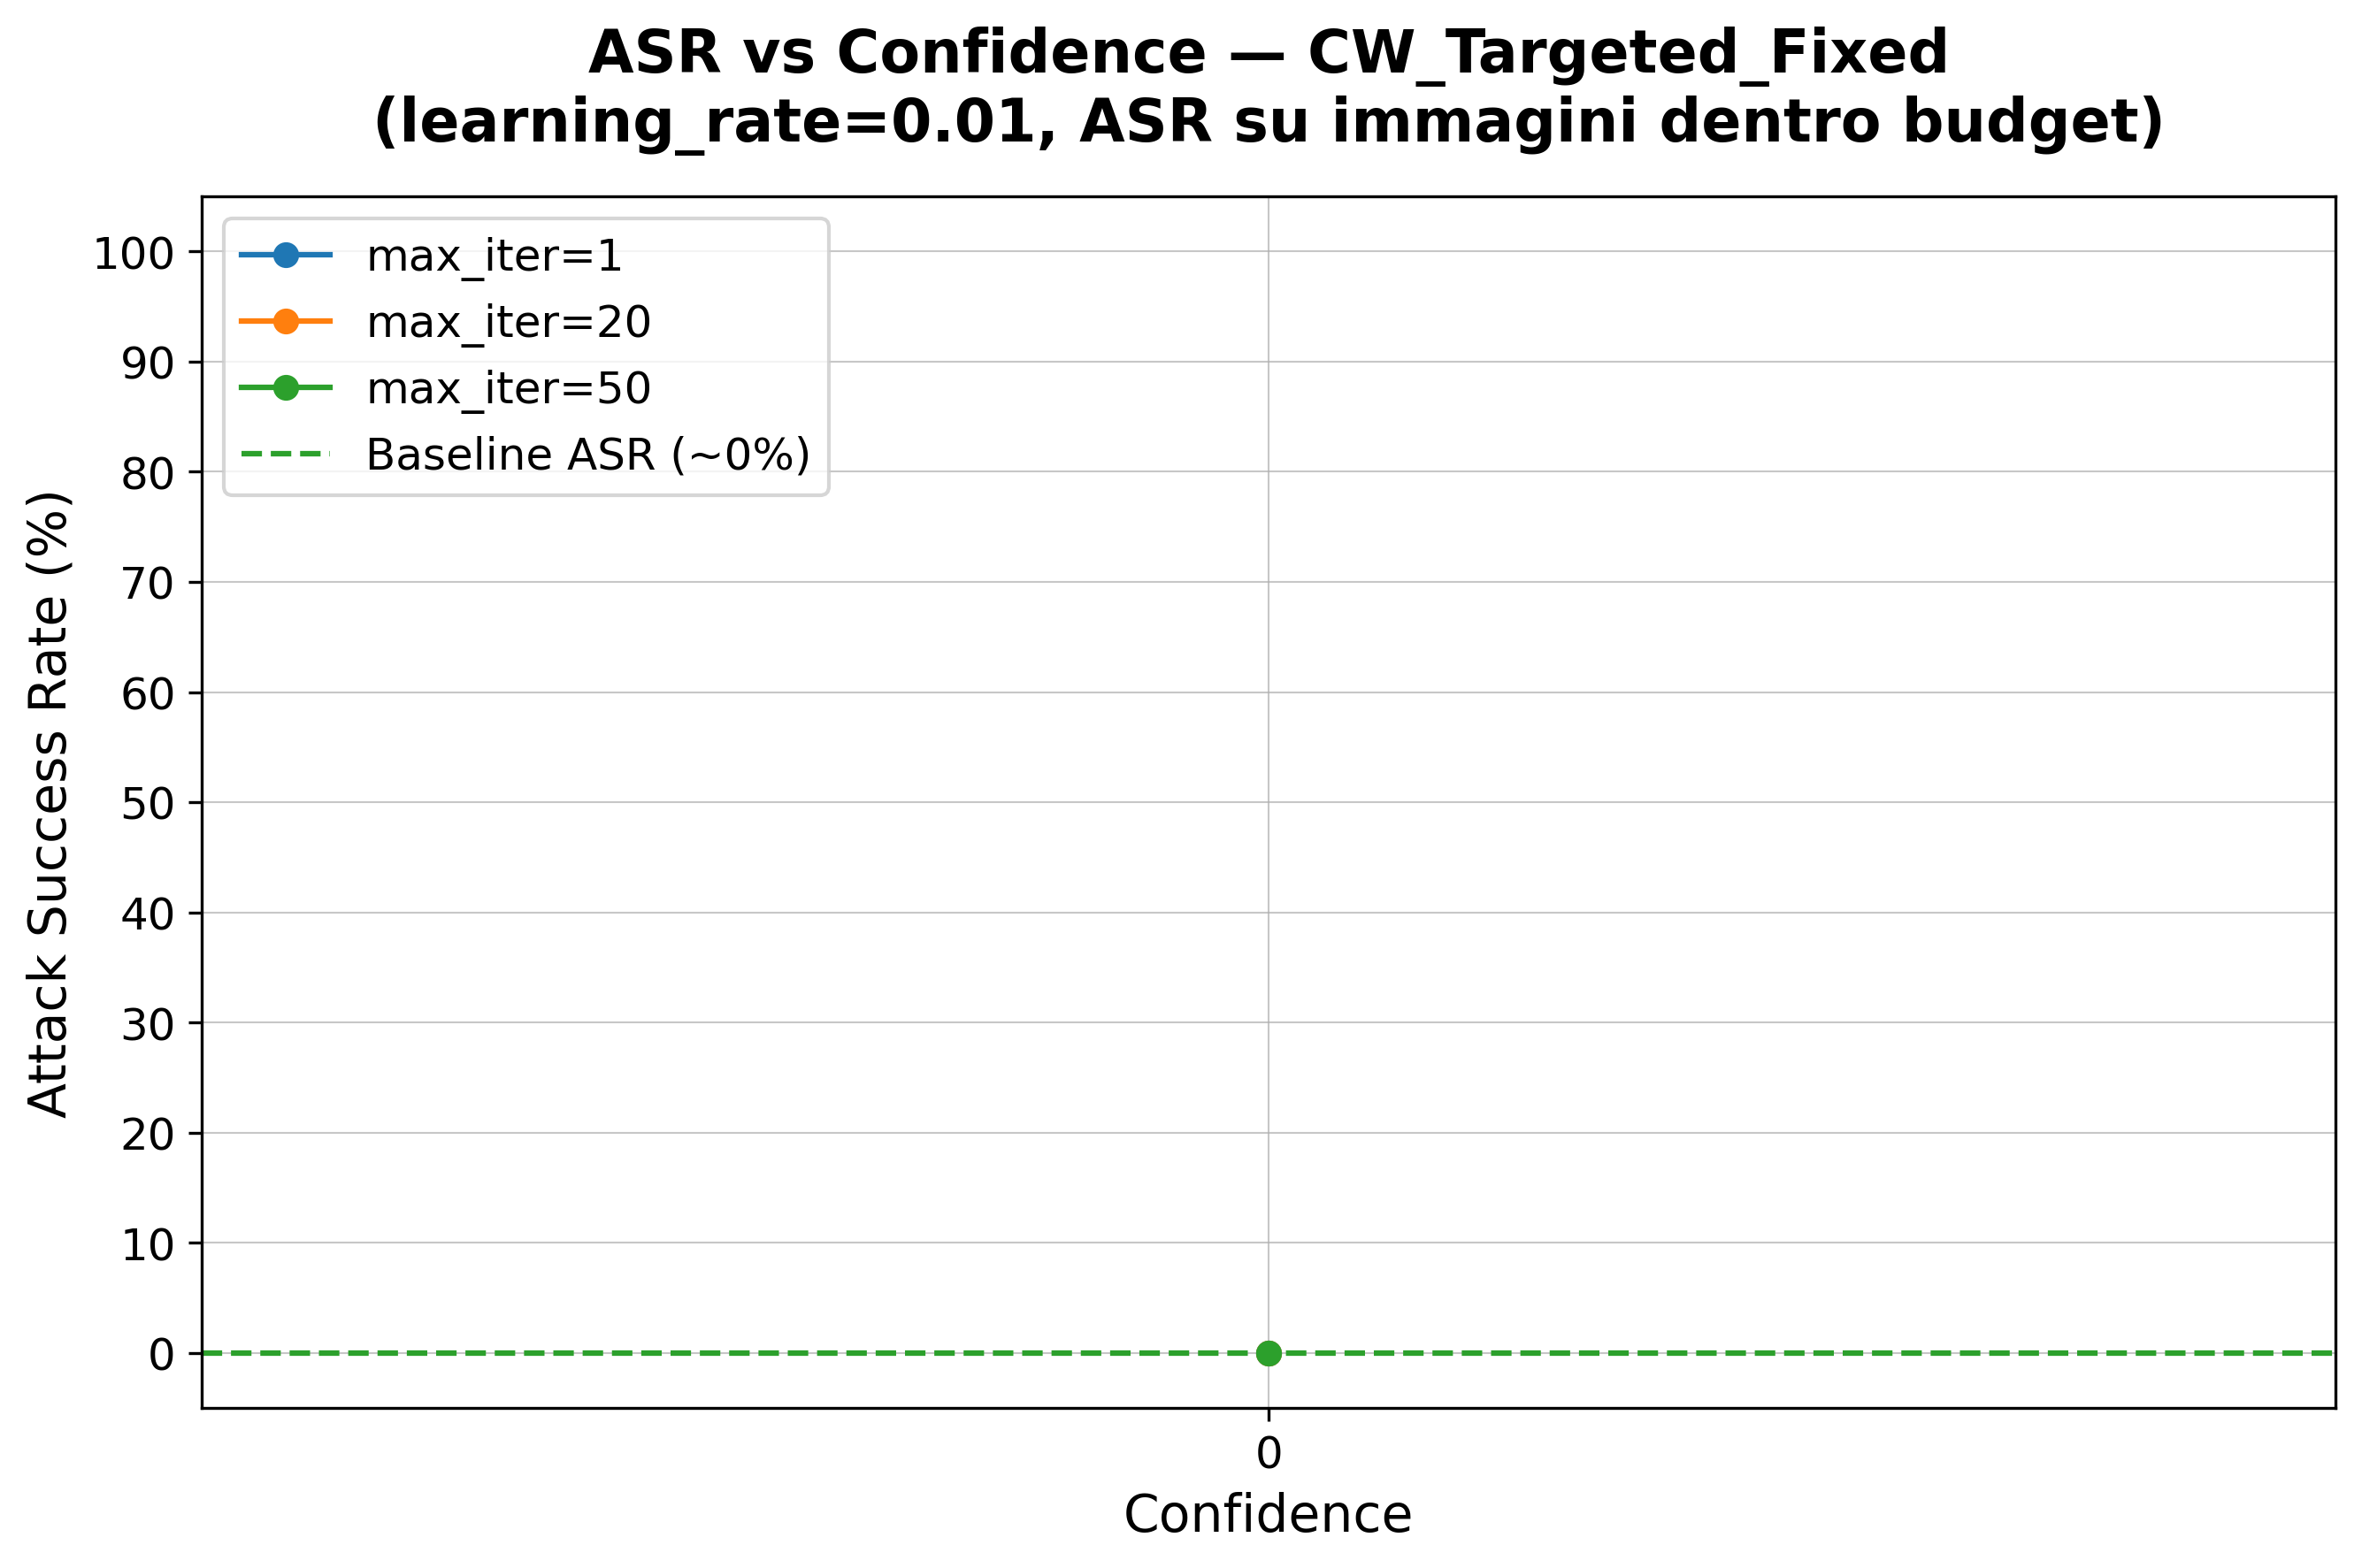
\includegraphics[width=\textwidth]{CW_Targeted/CW_Targeted_Fixed_asr_vs_conf_lr0_01.png}
                \caption{Learning rate 0.01}
                \label{fig:sec_fixed_cw_lr_0_01}
            \end{subfigure} \\ [1em] % Spazio verticale tra le righe
            
            % Sotto-figura 3 (In basso a sinistra)
            \begin{subfigure}[b]{0.55\textwidth}
                \centering
                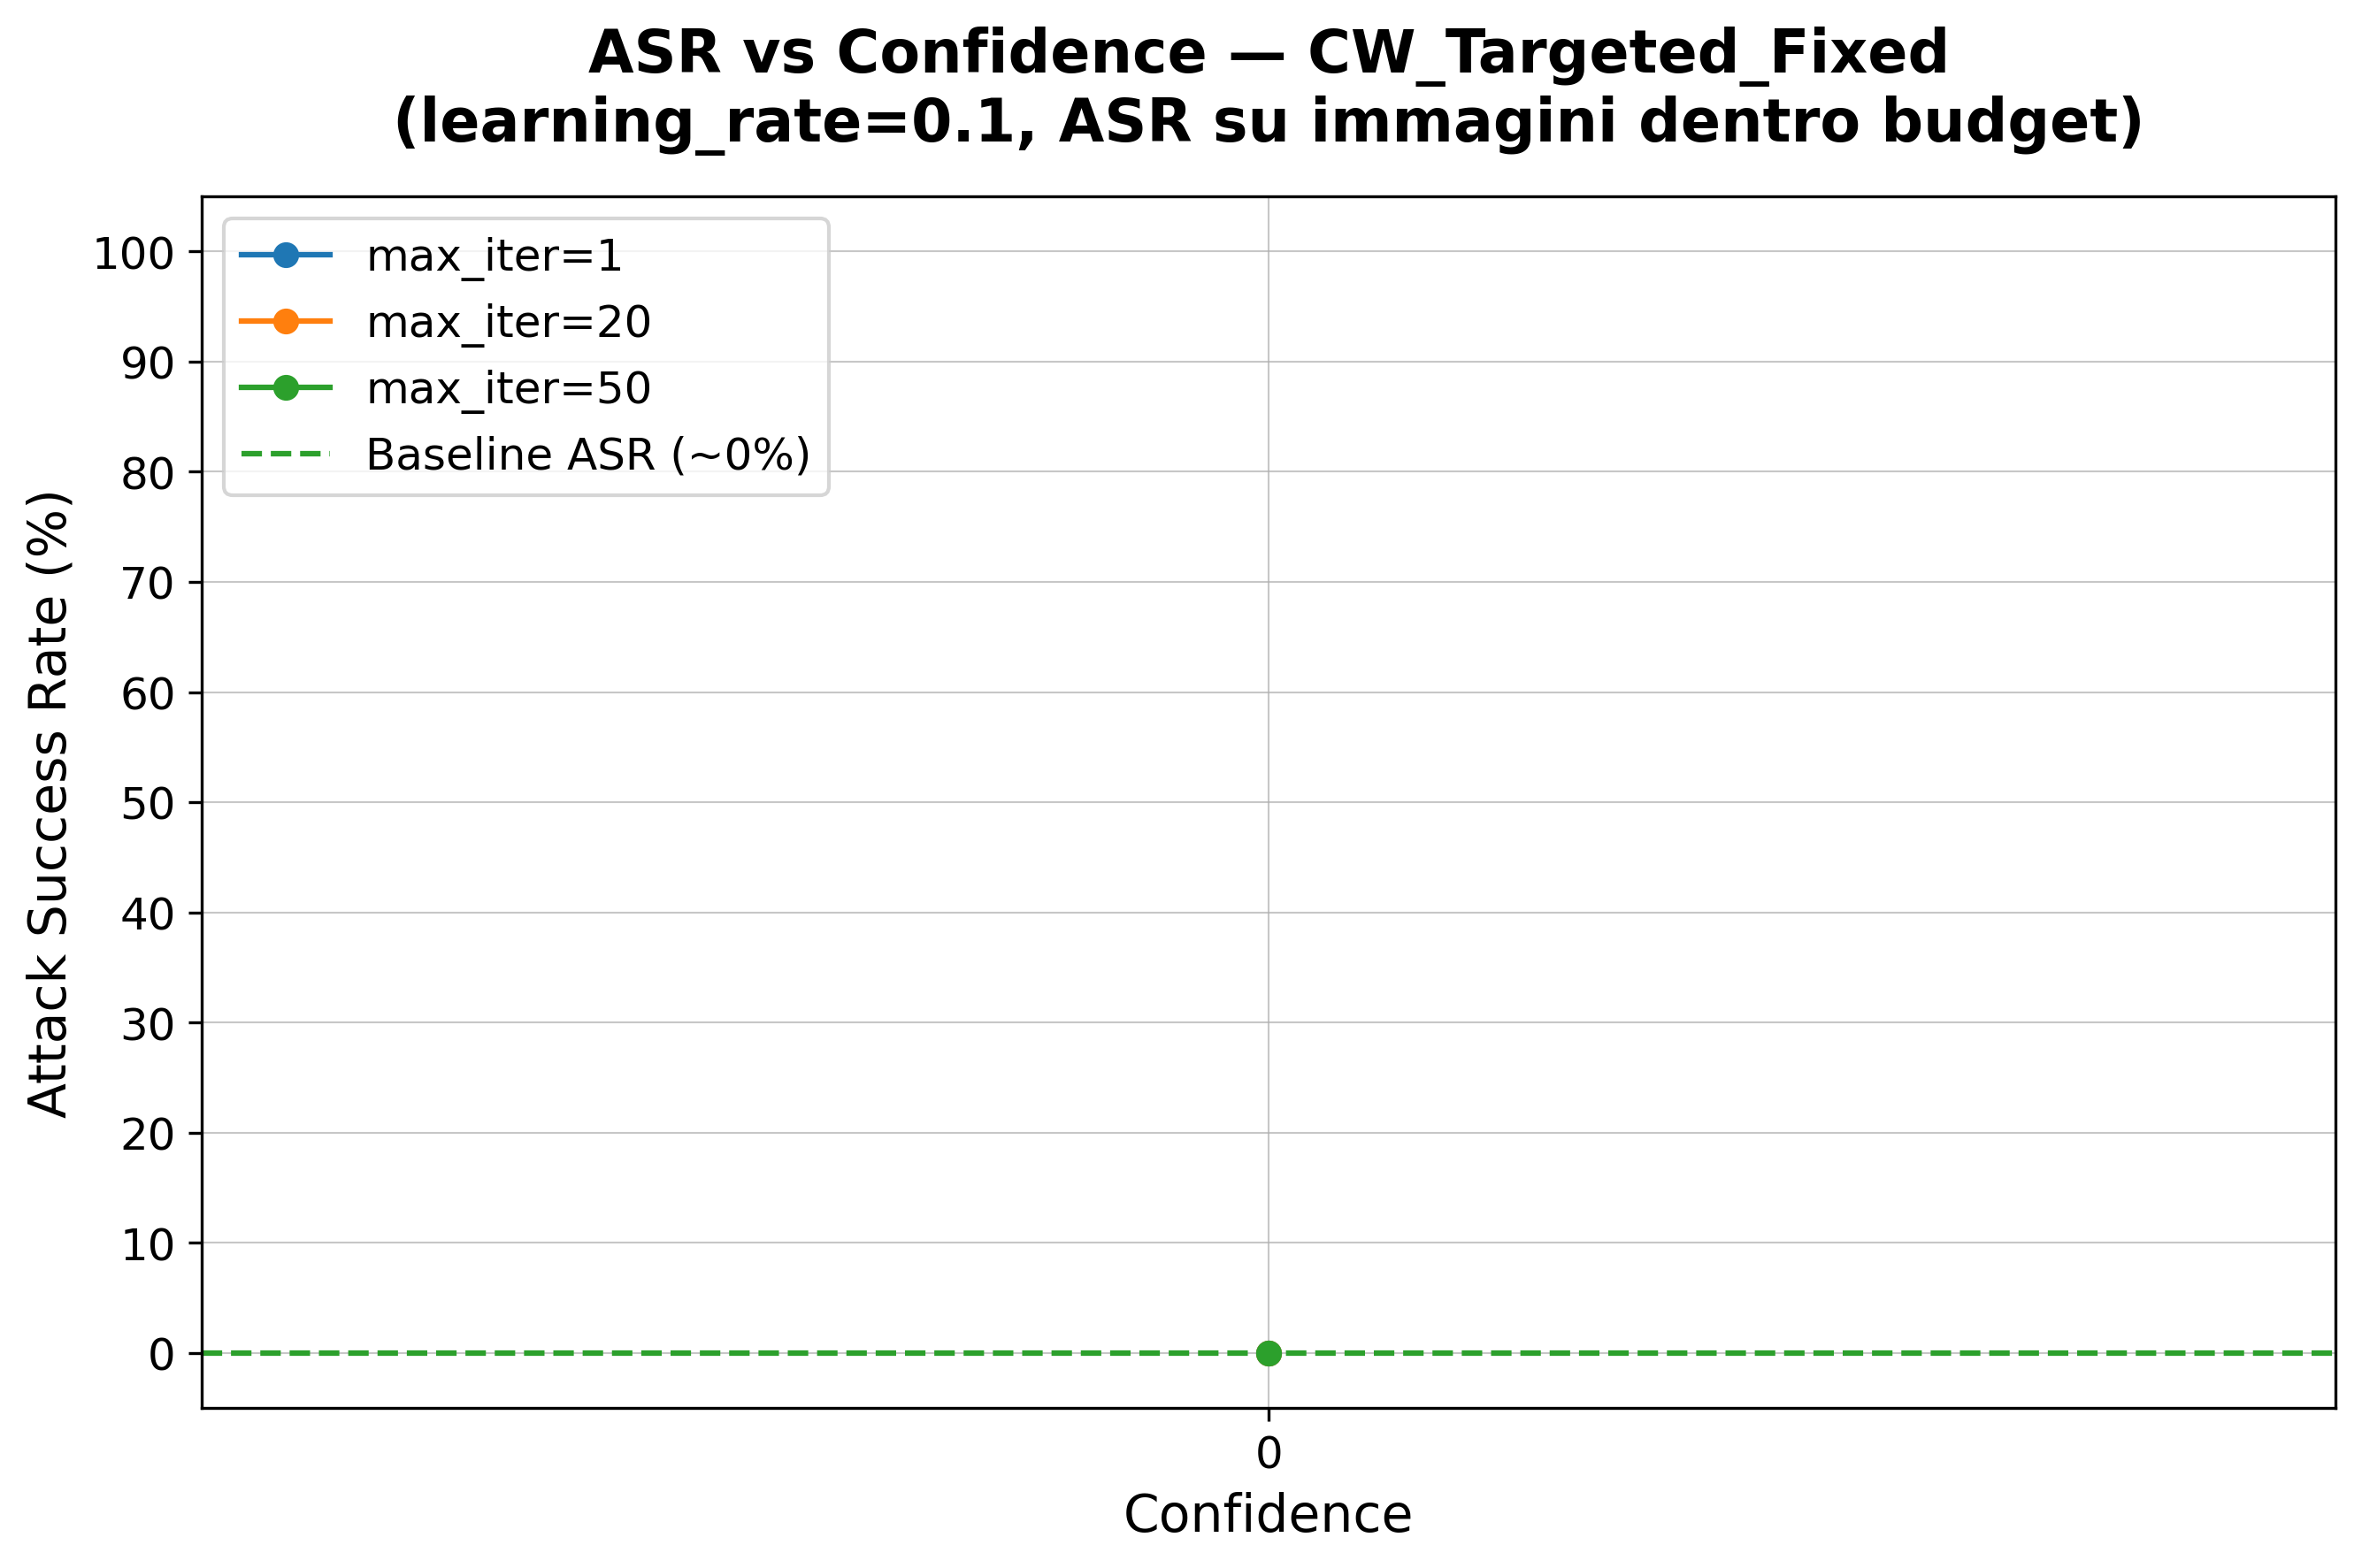
\includegraphics[width=\textwidth]{CW_Targeted/CW_Targeted_Fixed_asr_vs_conf_lr0_1.png}
                \caption{Learning rate 0.1}
                \label{fig:sec_fixed_cw_lr_0_1}
            \end{subfigure}
            &
            % Sotto-figura 4 (In basso a destra)
            \begin{subfigure}[b]{0.55\textwidth}
                \centering
                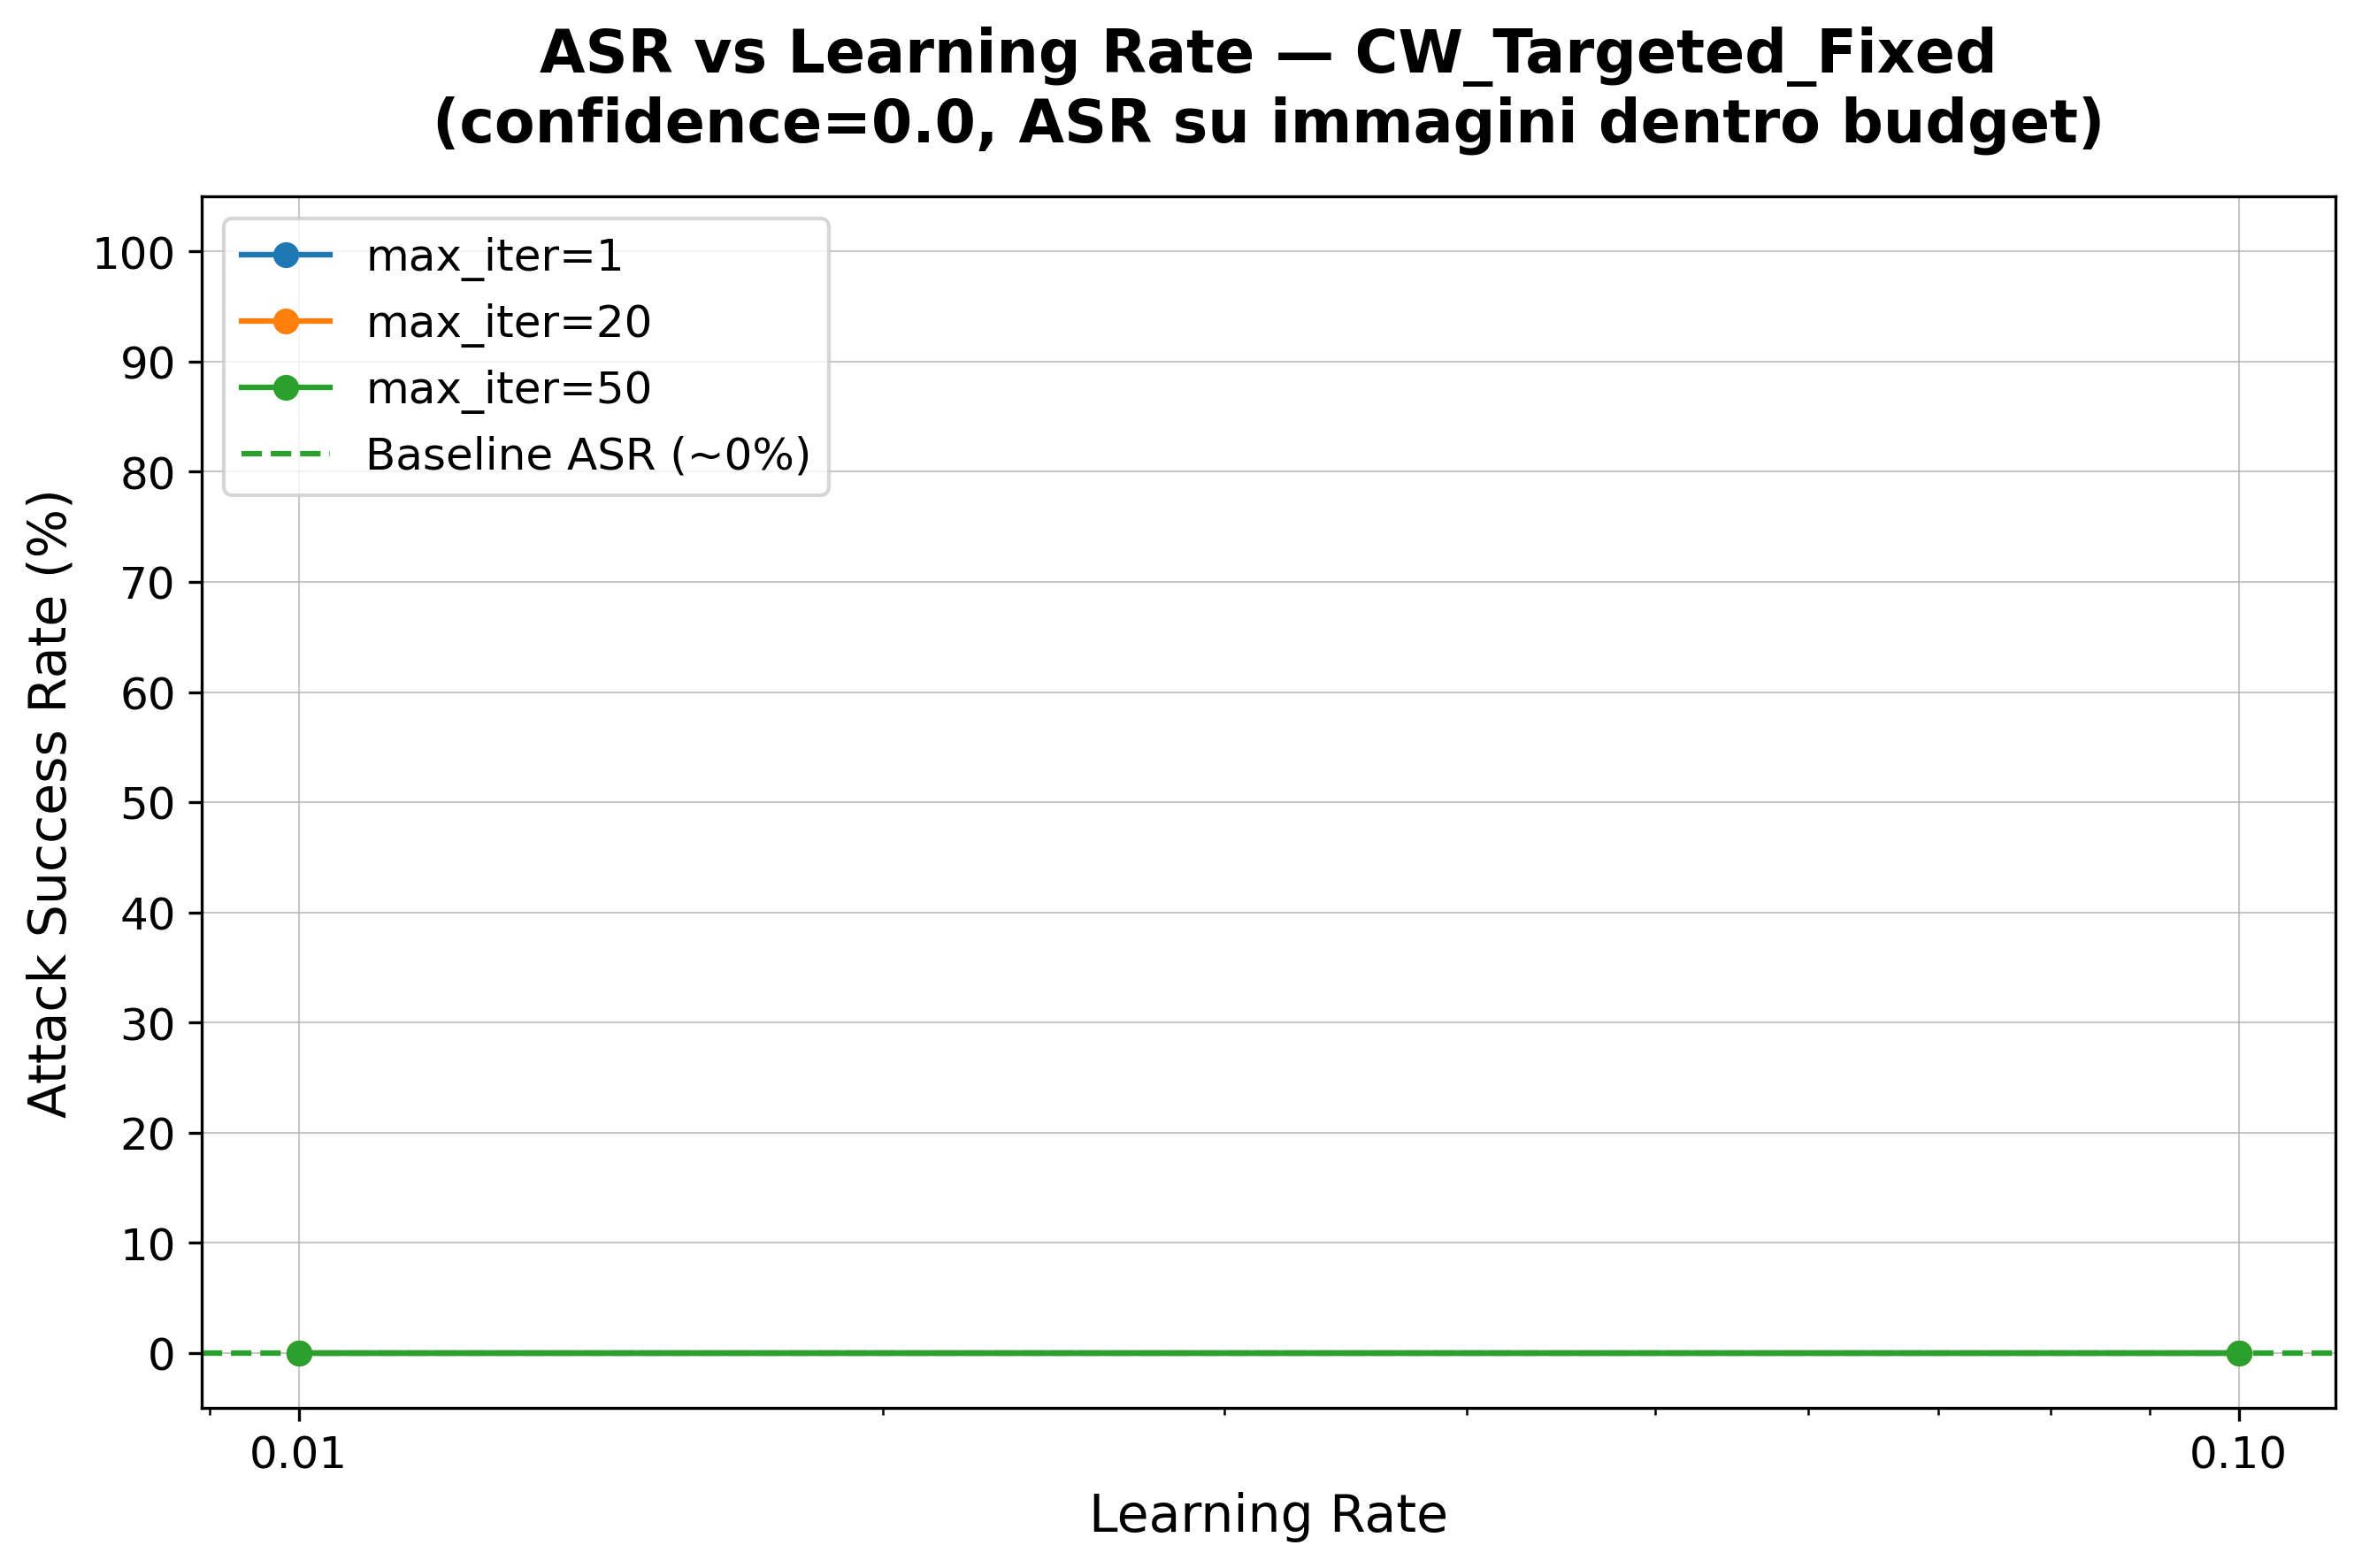
\includegraphics[width=\textwidth]{CW_Targeted/CW_Targeted_Fixed_asr_vs_lr_conf0_0.png}
                \caption{Confidence 0.0 e 0.1}
                \label{fig:sec_fixed_cw_conf_0_0}
            \end{subfigure}
            
        \end{tabular}
    }
    
    \caption{Risultati SEC per l'attacco CW Targeted (Fixed) in diverse configurazioni di Learning Rate e Confidence.}
    \label{fig:matrice_cw_targeted_fixed}
\end{figure}






\clearpage
\section{Transferability Analysis}
Un aspetto cruciale nella valutazione della robustezza dei sistemi di face recognition è la trasferibilità degli attacchi avversariali. Questa proprietà definisce la capacità di una perturbazione, originariamente calcolata per ingannare uno specifico modello (NN1), di mantenere la propria efficacia malevola anche contro un modello differente (NN2), permettendo all'attaccante di sfruttare vulnerabilità condivise tra architetture simili.

In questo capitolo viene simulato uno scenario di attacco di tipo black-box. In tale contesto, si assume che l'attaccante non abbia alcun accesso all'architettura interna, ai parametri o ai gradienti del modello NN2, conoscendone esclusivamente il dominio applicativo.
Per aggirare questa limitazione, l'attaccante impiega il modello fornito NN1 come modello surrogato, generando quindi le immagini avversariali basandosi su questo modello.
Le immagini avversariali così prodotte vengono successivamente testate su NN2 per verificare se le perturbazioni applicate mantengono la propria efficacia, riuscendo a ingannare un modello differente da quello per cui sono state originariamente progettate.

\subsection{Error-Generic Attack}



\subsubsection{Fast Gradient Sign Method (FGSM)}

In questa sezione viene valutata l'accuratezza del modello NN2 sugli esempi avversariali generati tramite l'attacco FGSM contro NN1, analizzandone il comportamento al variare di $\epsilon$. 

Per visualizzare chiaramente l'impatto dell'attacco, i risultati sono presentati attraverso una Security Evaluation Curve comparativa in Figura \ref{fig:fgsm_transferability_untargeted}. Questo grafico rappresenta l'accuracy di NN1 e di NN2, testati con diversi insiemi di immagini avversariali. Ciasun insieme è riferito a un diverso valore di $\epsilon$. Vengono testate prima le immagini con $\epsilon = 0.01$, poi con $\epsilon = 0.1$, e cosi via, fino a raggiungere il budget massimo di $\epsilon = 0.1$.
\begin{figure}[htbp]
    \centering
    % Regola il parametro width (es. 0.8\textwidth) per ingrandire o rimpicciolire l'immagine
    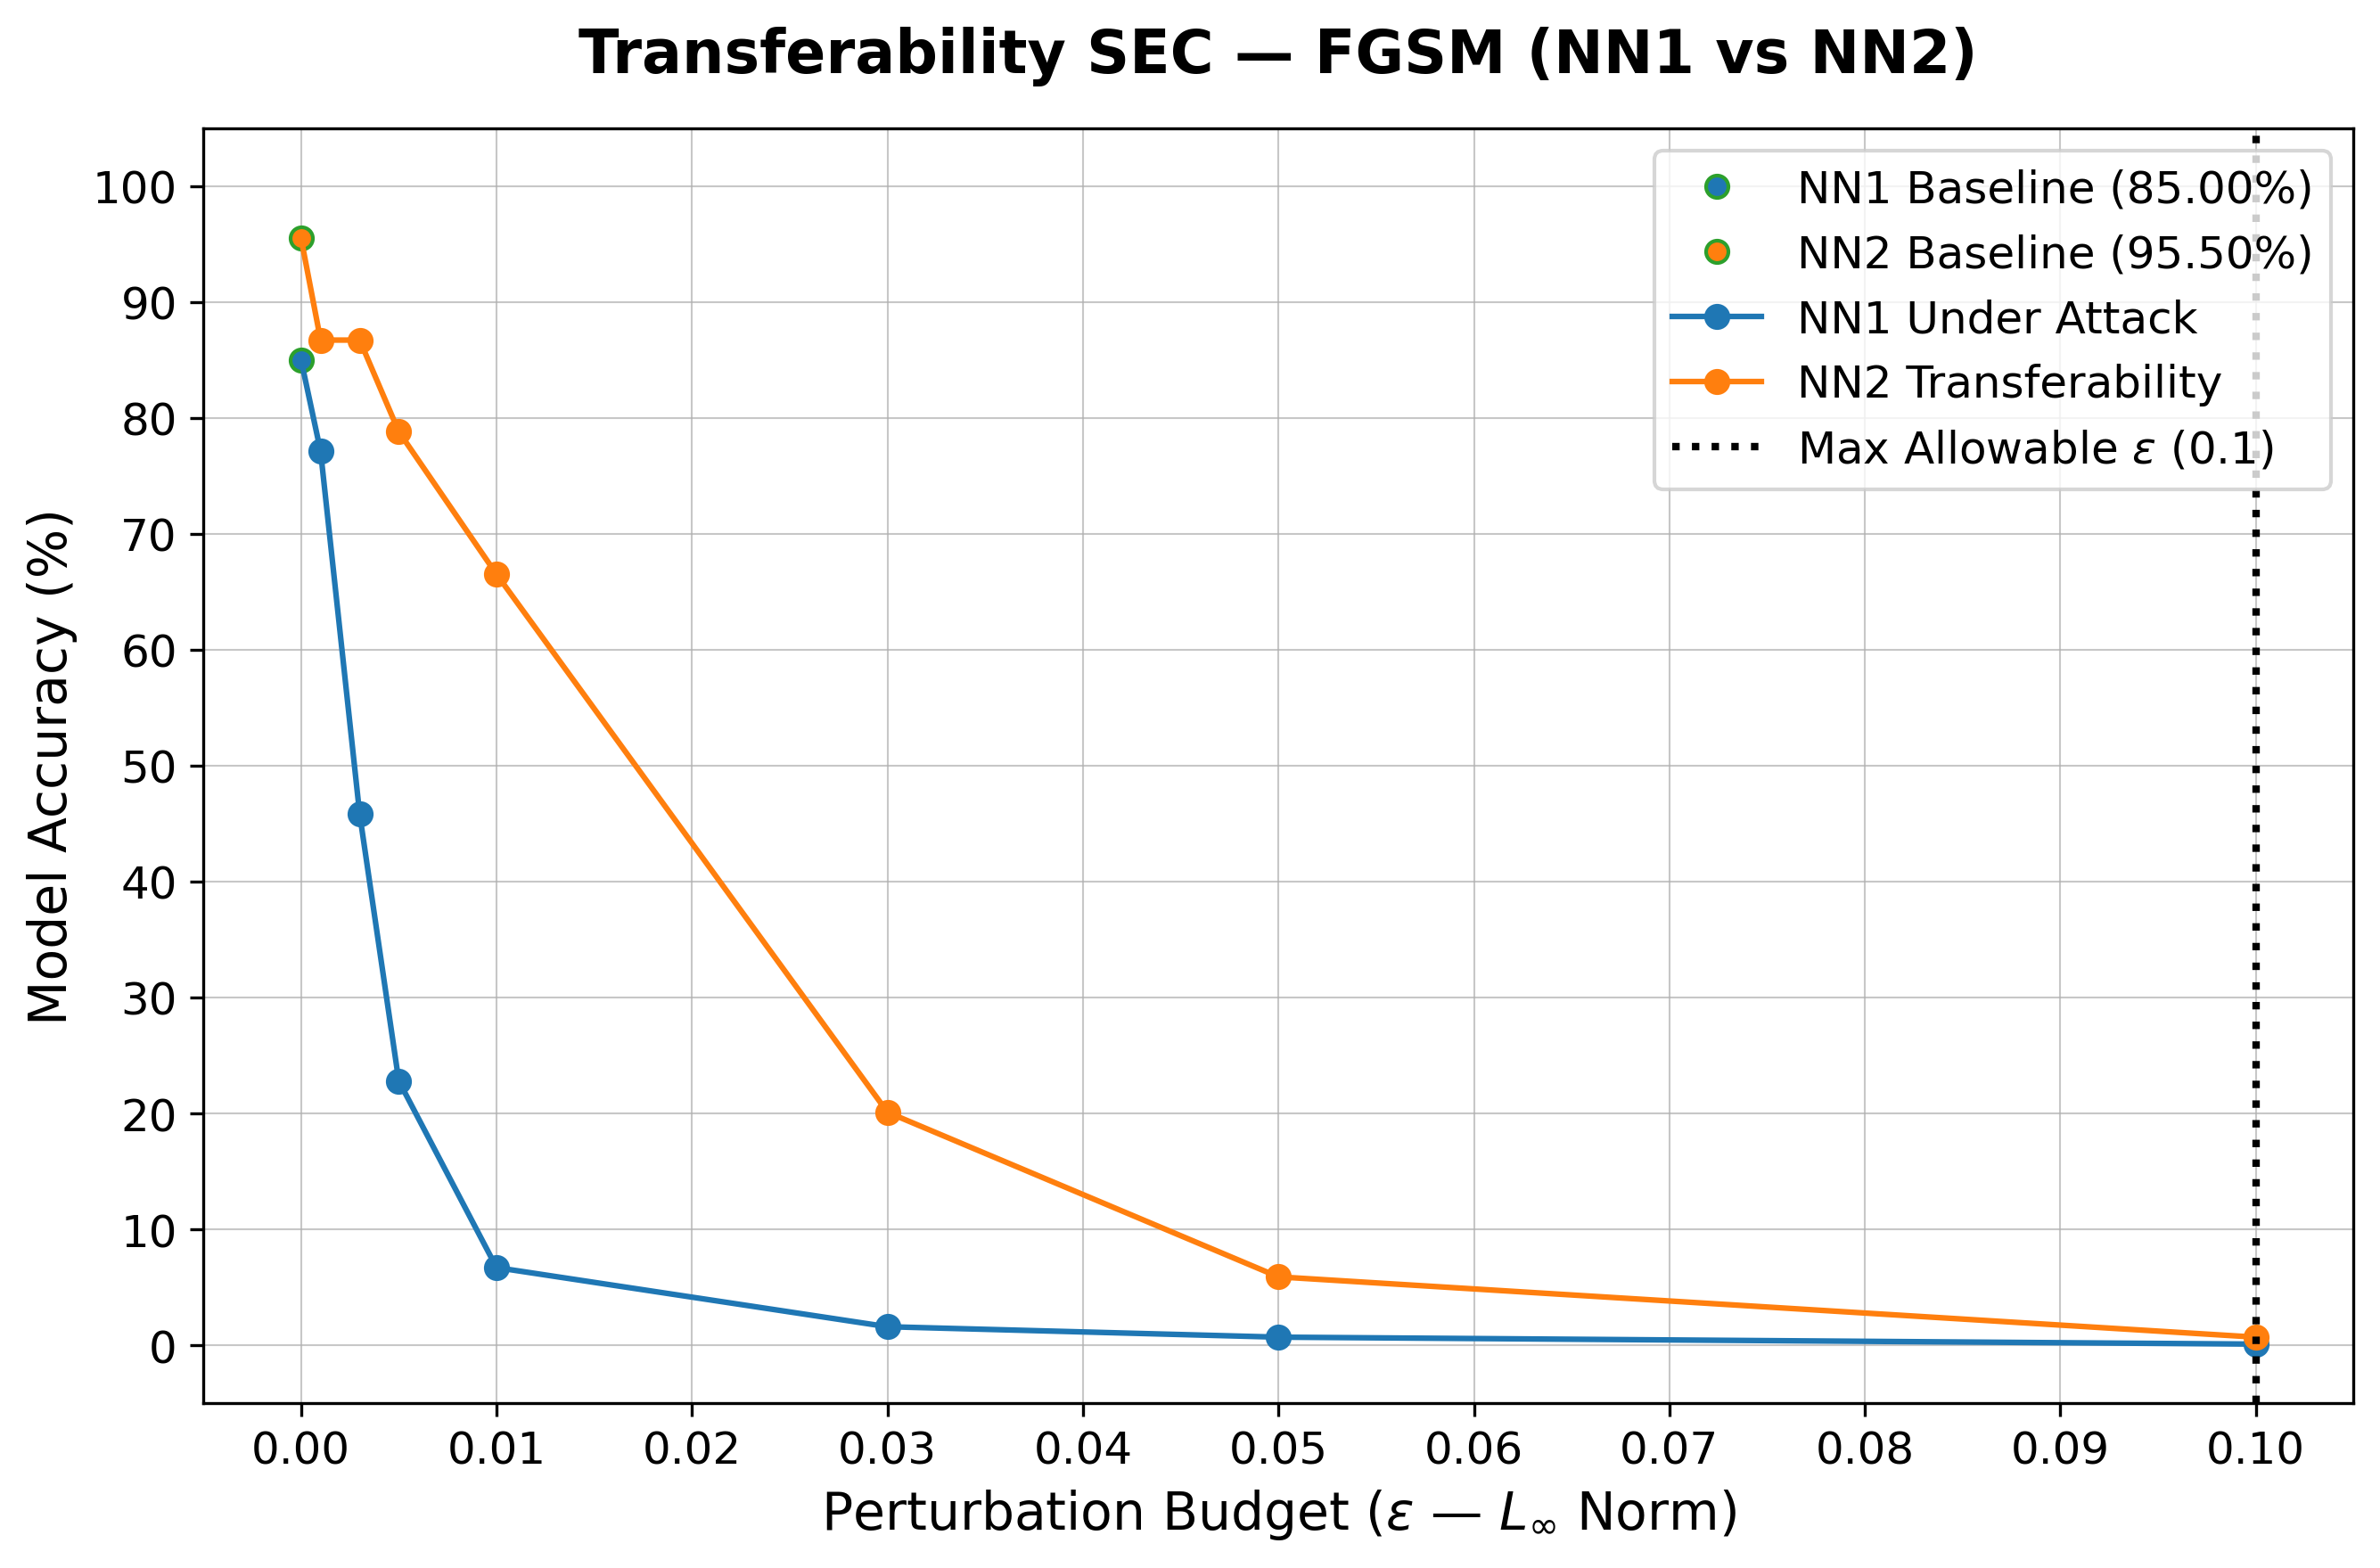
\includegraphics[width=0.8\textwidth]{./Transferability/untargeted/FGSM/image.png}
    \caption{SEC comparativa per l'attacco FGSM Untargeted.}
    \label{fig:fgsm_transferability_untargeted}
\end{figure}

Dal grafico emerge innanzitutto una differenza nelle prestazioni di base dei due modelli su immagini non perturbate ($\epsilon$=0.00). Il modello bersaglio NN2 dimostra una capacità di generalizzazione superiore, registrando un'accuratezza del 95.50\%, rispetto all'85.00\% del modello surrogato NN1.
Dall'analisi del grafico è possibile evidenziare i seguenti aspetti chiave:
\begin{itemize}
    \item L'accuratezza del secondo modello decresce progressivamente all'aumentare di $\epsilon$, confermando che anche l'architettura \textit{black-box} (NN2) subisce l'effetto dell'attacco originato sul modello surrogato.
    \item Per valori di perturbazione contenuti, NN2 mostra una robustezza superiore rispetto a NN1.
    \item In corrispondenza del valore $\epsilon = 0.05$, le due curve tendono a convergere verso gli stessi valori di accuracy. Questo indica che i modelli si comportano in maniera simile con $\epsilon \geq 0.05$.
\end{itemize}
I dati numerici completi sono riportati nella Tabella \ref{tab:fgsm_tab_unt_transferability}, che mostra inoltre il \textit{Transfer Gap}, ovvero la differenza di accuracy tra NN2 e NN1 per ogni valore di $\epsilon$.
\begin{table}[htbp]
    \centering
    \vspace{0.2cm}
    \begin{tabular}{cccc}
        \toprule
        \textbf{($\epsilon$)} & \textbf{Accuracy NN2} & \textbf{Accuracy NN1} & \textbf{Gap} \\
        \midrule
        0.001 & 86.70\% & 77.10\% & +9.60\% \\
        0.003 & 86.70\% & 45.80\% & +40.90\% \\
        0.005 & 78.80\% & 22.80\% & +56.00\% \\
        0.010 & 66.50\% &  6.70\% & \textbf{+59.80\%} \\
        0.030 & 20.10\% &  1.60\% & +18.50\% \\
        0.050 &  5.90\% &  0.70\% & +5.20\% \\
        0.100 &  0.70\% &  0.10\% & +0.60\% \\
        \bottomrule
    \end{tabular}
    \caption{Risultati di transferabilità per l'attacco FGSM Untargeted.}
    \label{tab:fgsm_tab_unt_transferability}
\end{table}

Il Transfer Gap, calcolato come $\text{Acc}_{NN2} - \text{Acc}_{NN1}$, quantifica la differenza di accuracy tra i due modelli per ogni valore di $\epsilon$: un valore basso indica una bassa transferibilità.
Per valori di perturbazione ridotti ($\epsilon \leq 0.010$), il gap raggiunge 
il suo massimo ($+59.80\%$ per $\epsilon = 0.010$), indicando 
che l'attacco, pur essendo efficace su NN1, si trasferisce solo parzialmente su NN2.
Al crescere di $\epsilon$, il gap si riduce progressivamente fino a quasi annullarsi 
($+0.60\%$ per $\epsilon = 0.100$). Questo indica che NN2 è robusta fino a circa $\epsilon = 0.01$. Tuttavia, aumentando le perturbazioni, aumenta anche la trasferibilità, riuscendo a compromettere con successo NN2.


\subsubsection{Basic Iterative Method (BIM)}

In questa sezione viene valutata l'accuracy del modello NN2 sugli esempi avversariali generati tramite l'attacco BIM contro NN1, analizzandone il comportamento al variare di $\epsilon$ e di \texttt{max\_iter}. 

Per visualizzare chiaramente l'impatto dell'attacco, i risultati sono presentati attraverso una Security Evaluation Curve comparativa in Figura \ref{fig:bim_transferability_untargeted}. Questo grafico rappresenta l'accuracy di NN1 e di NN2, ottenute testando con diversi insiemi di immagini avversariali.
A parità di $\epsilon$, ciascun insieme è riferito a un diverso valore di \texttt{max\_iter}.

\begin{figure}[H]
    \centering
    % Regola il parametro width (es. 0.8\textwidth) per ingrandire o rimpicciolire l'immagine
    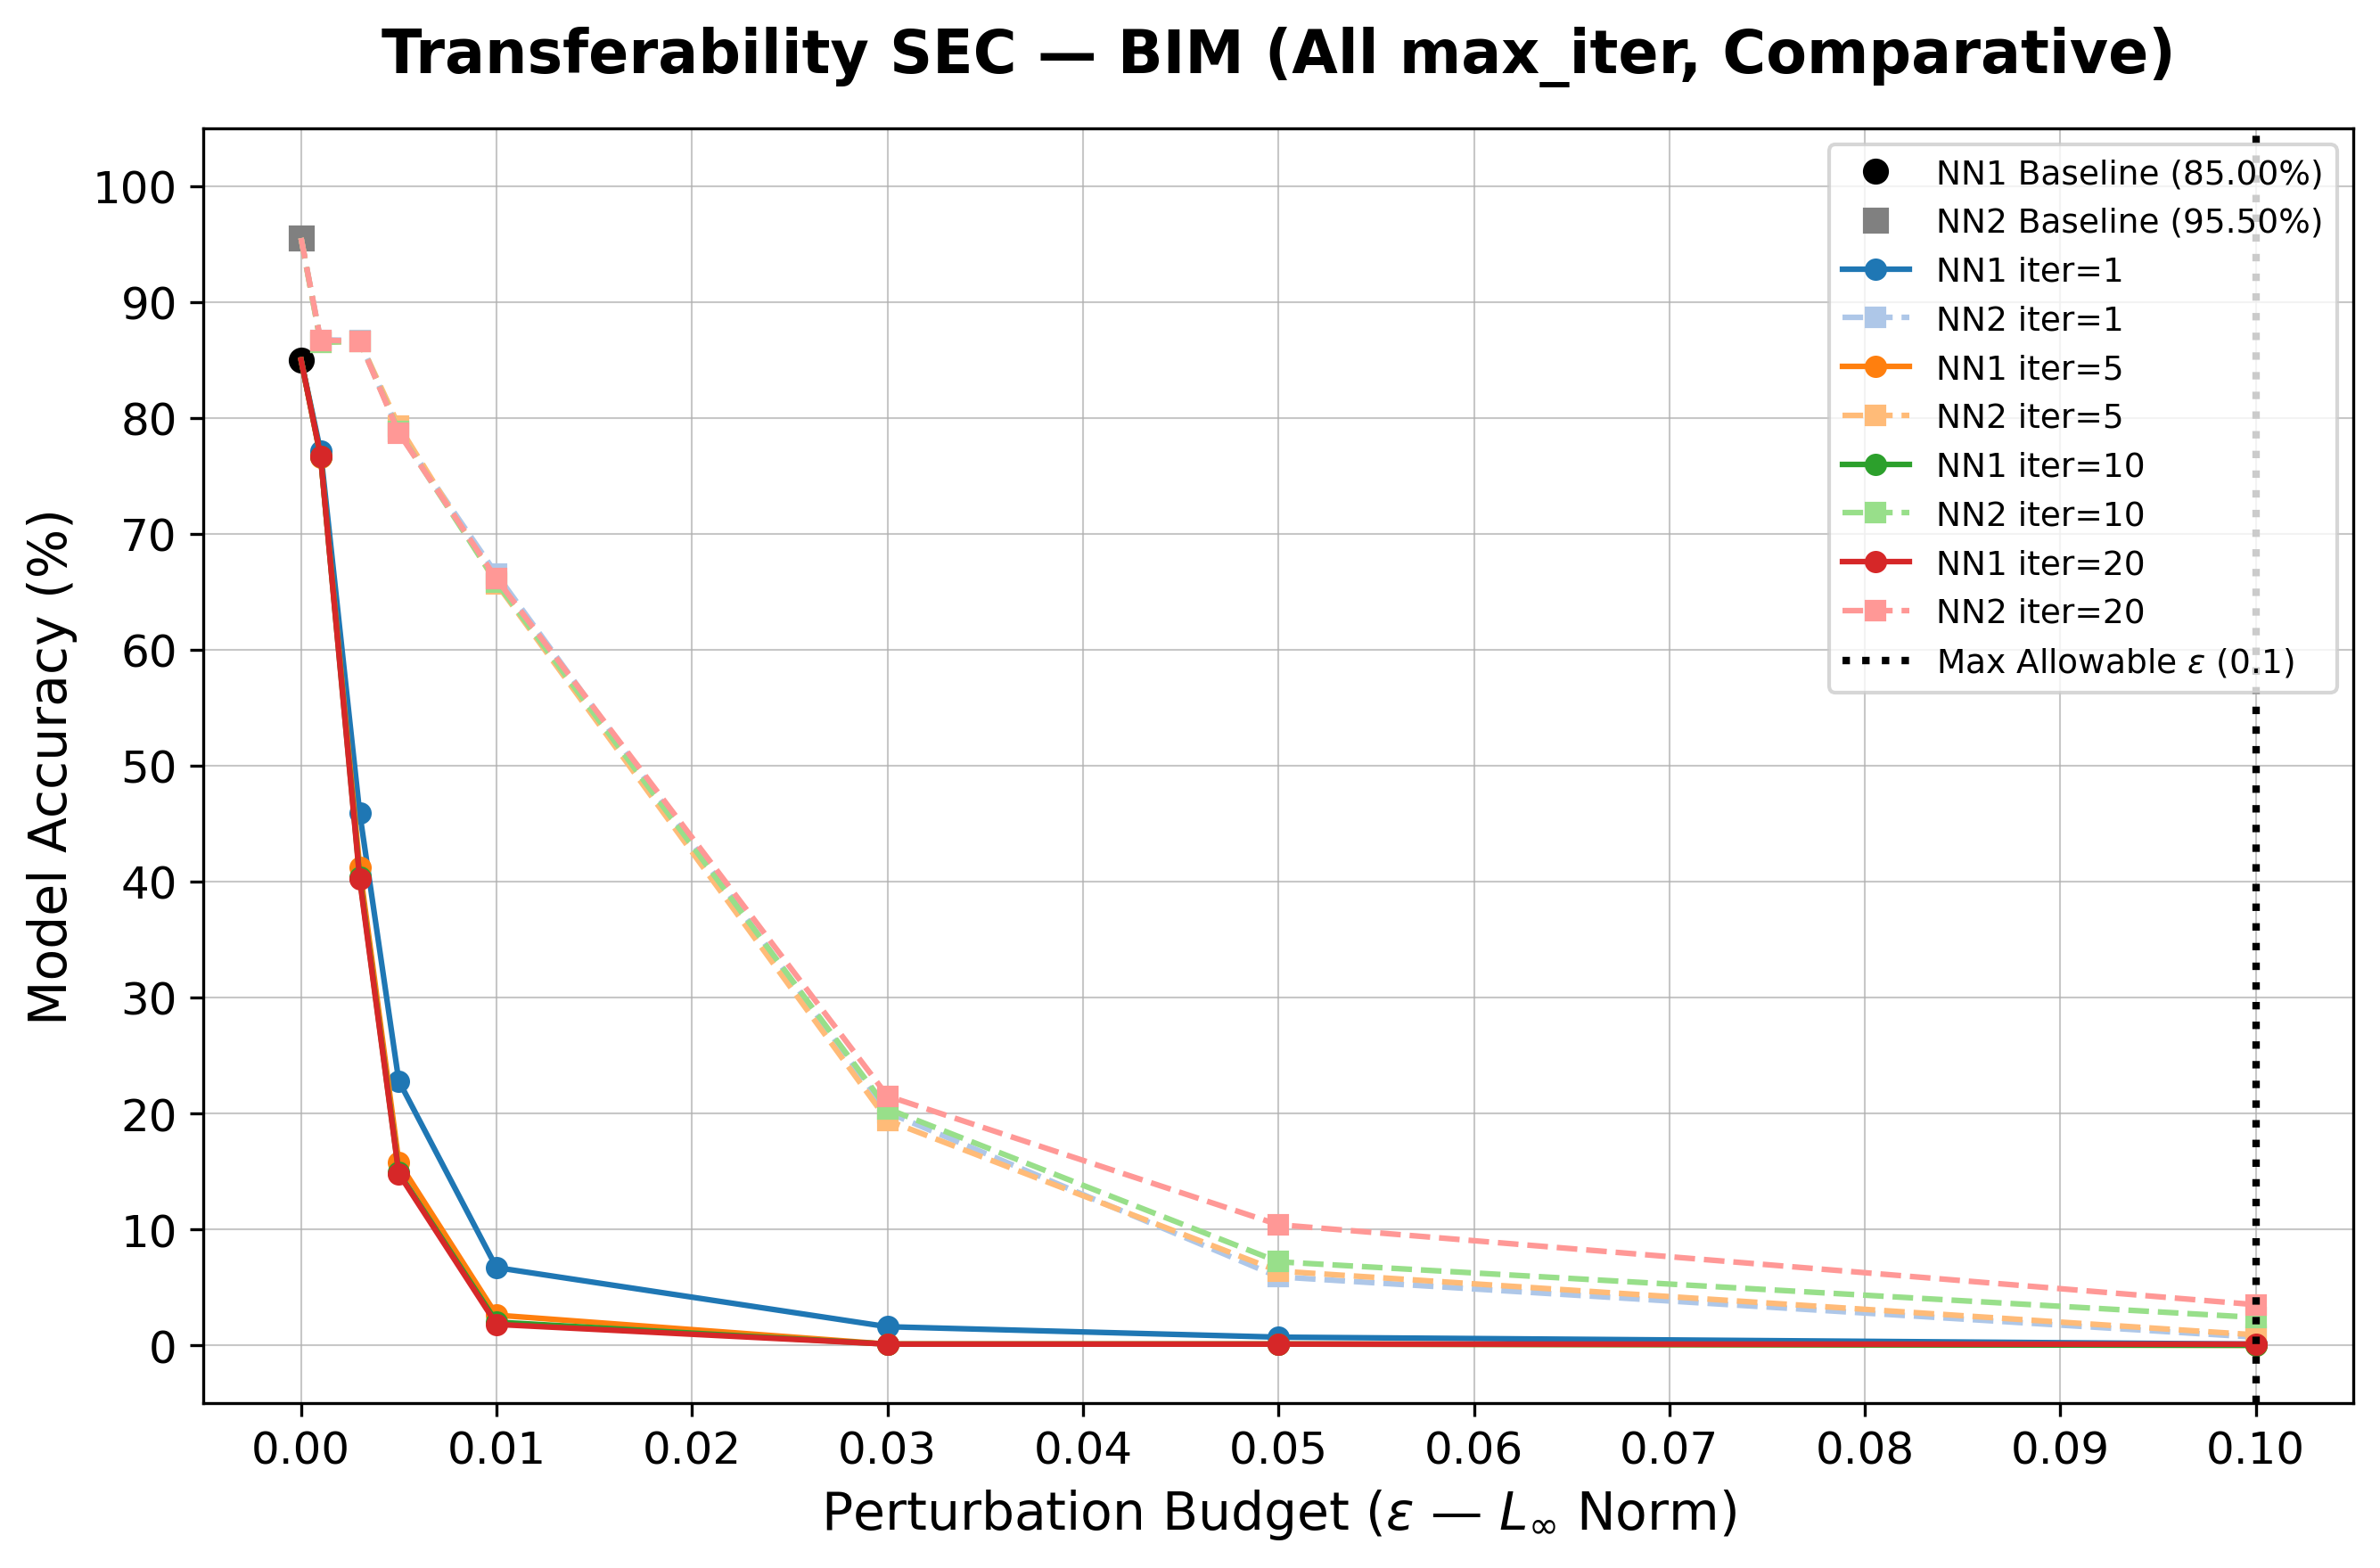
\includegraphics[width=0.8\textwidth]{./Transferability/untargeted/BIM/image.png}
    \caption{SEC comparativa per l'attacco BIM.}
    \label{fig:bim_transferability_untargeted}
\end{figure}

Dall'analisi in Figura \ref{fig:bim_transferability_untargeted}, emergono le seguenti considerazioni:

\begin{itemize}
    \item All'aumentare di \texttt{max\_iter}, l'accuracy di NN1 crolla più rapidamente al crescere 
    di $\epsilon$. Per \texttt{iter=10} e \texttt{iter=20}, NN1 si azzera già 
    intorno a $\epsilon = 0.01$, confermando che BIM diventa più efficace sul modello surrogato NN1 con l'aumentare delle iterazioni.

    \item Le curve tratteggiate di NN2 si mantengono al di sopra delle corrispondenti curve di NN1, dimostrando che NN2 è piu' robusto rispettto a NN1.

    \item Il comportamento con una sola iterazione è assimilabile a quello dell'attacco FGSM, quindi valgono le considerazioni trattate in precedenza.


\end{itemize}

\begin{table}[htbp]
    \centering
    \setlength{\tabcolsep}{12pt} % <-- AUMENTA QUESTO VALORE (es. 10pt, 12pt, 15pt)
    \vspace{0.2cm}
    \makebox[\textwidth][c]{
    \begin{tabular}{c | cc | cc | ccc}
        \hline
        & \multicolumn{2}{c|}{\textbf{max\_iter = 5}}
        & \multicolumn{2}{c|}{\textbf{max\_iter = 10}}
        & \multicolumn{3}{c}{\textbf{max\_iter = 20}} \\
        \hline
        \textbf{$\epsilon$}
        & \textbf{NN2} & \textbf{NN1}
        & \textbf{NN2} & \textbf{NN1}
        & \textbf{NN2} & \textbf{NN1} & \textbf{Gap} \\
        \hline
        0.010 & 65.70\% & 2.60\% & 65.70\% & 2.00\% & 66.00\% & 1.80\% & +64.20\% \\
        0.030 & 19.40\% & 0.10\% & 20.40\% & 0.10\% & 21.50\% & 0.10\% & +21.40\% \\
        0.050 &  6.40\% & 0.10\% &  7.20\% & 0.10\% & 10.40\% & 0.10\% & +10.30\% \\
        0.100 &  0.90\% & 0.00\% &  2.40\% & 0.00\% &  3.50\% & 0.10\% & +3.40\% \\
        \hline
    \end{tabular}
    }
    \caption{Risultati di transferabilità per l'attacco BIM Untargeted.}
    \label{tab:bim_unt_table}
\end{table}



Dai risultati in Tabella \ref{tab:bim_unt_table} emerge che l'utilizzo di esempi avversariali generati con 
un valore di \texttt{max\_iter} più elevato non garantisce un miglioramento 
significativo dell'efficacia dell'attacco nei confronti di NN2. Infatti, 
confrontando le accuratezze di NN2 al variare di \texttt{max\_iter} a parità 
di $\epsilon$, l'aumento medio di accuracy tra \texttt{max\_iter=5} e 
\texttt{max\_iter=20} è di circa il $2\%$. Questo risultato conferma che incrementare il numero di iterazioni dell'attacco BIM, 
non porta a una migliore transferibilità degli attacchi su NN2.

Il Transfer Gap riportato per \texttt{max\_iter=20} conferma ulteriormente questo 
comportamento: nonostante NN1 sia quasi completamente compromesso in tutte le 
configurazioni, il Gap rimane elevato per valori di perturbazione contenuti, 
raggiungendo il $+64.20\%$ per $\epsilon = 0.010$. Al crescere di $\epsilon$, 
il Gap si riduce progressivamente fino al $+3.40\%$ per $\epsilon = 0.100$, indicando una \textbf{crescente transferibilità} 
dell'attacco: perturbazioni piu' marcate riescono a compromettere NN2 favorendo la trasferibilità dei rispettivi campioni avversariali.



\subsubsection{Projected Gradient Descent (PGD)}
In questa sezione viene valutata l'accuracy del modello NN2 sugli esempi 
avversariali generati tramite l'attacco PGD contro NN1, analizzandone il 
comportamento al variare di $\epsilon$, del numero di iterazioni 
\texttt{max\_iter} e del numero di inizializzazioni casuali \texttt{nri} 
(\textit{number of random init}).

Poiché la combinazione di tutti i valori di \texttt{max\_iter} e \texttt{nri} 
genera un numero elevato di configurazioni, i risultati sono sintetizzati in 
due Security Evaluation Curve comparative. La prima, riportata in 
Figura~\ref{fig:pgd_transferability_untargeted}, isola l'effetto del parametro 
\texttt{nri} fissando \texttt{max\_iter} al valore massimo $40$; essa 
rappresenta l'accuracy di NN1 e di NN2 ottenute testando i diversi insiemi di 
immagini avversariali generati con \texttt{nri} pari a $0$, $1$, $3$ e $5$.

\begin{figure}[htbp]
    \centering
    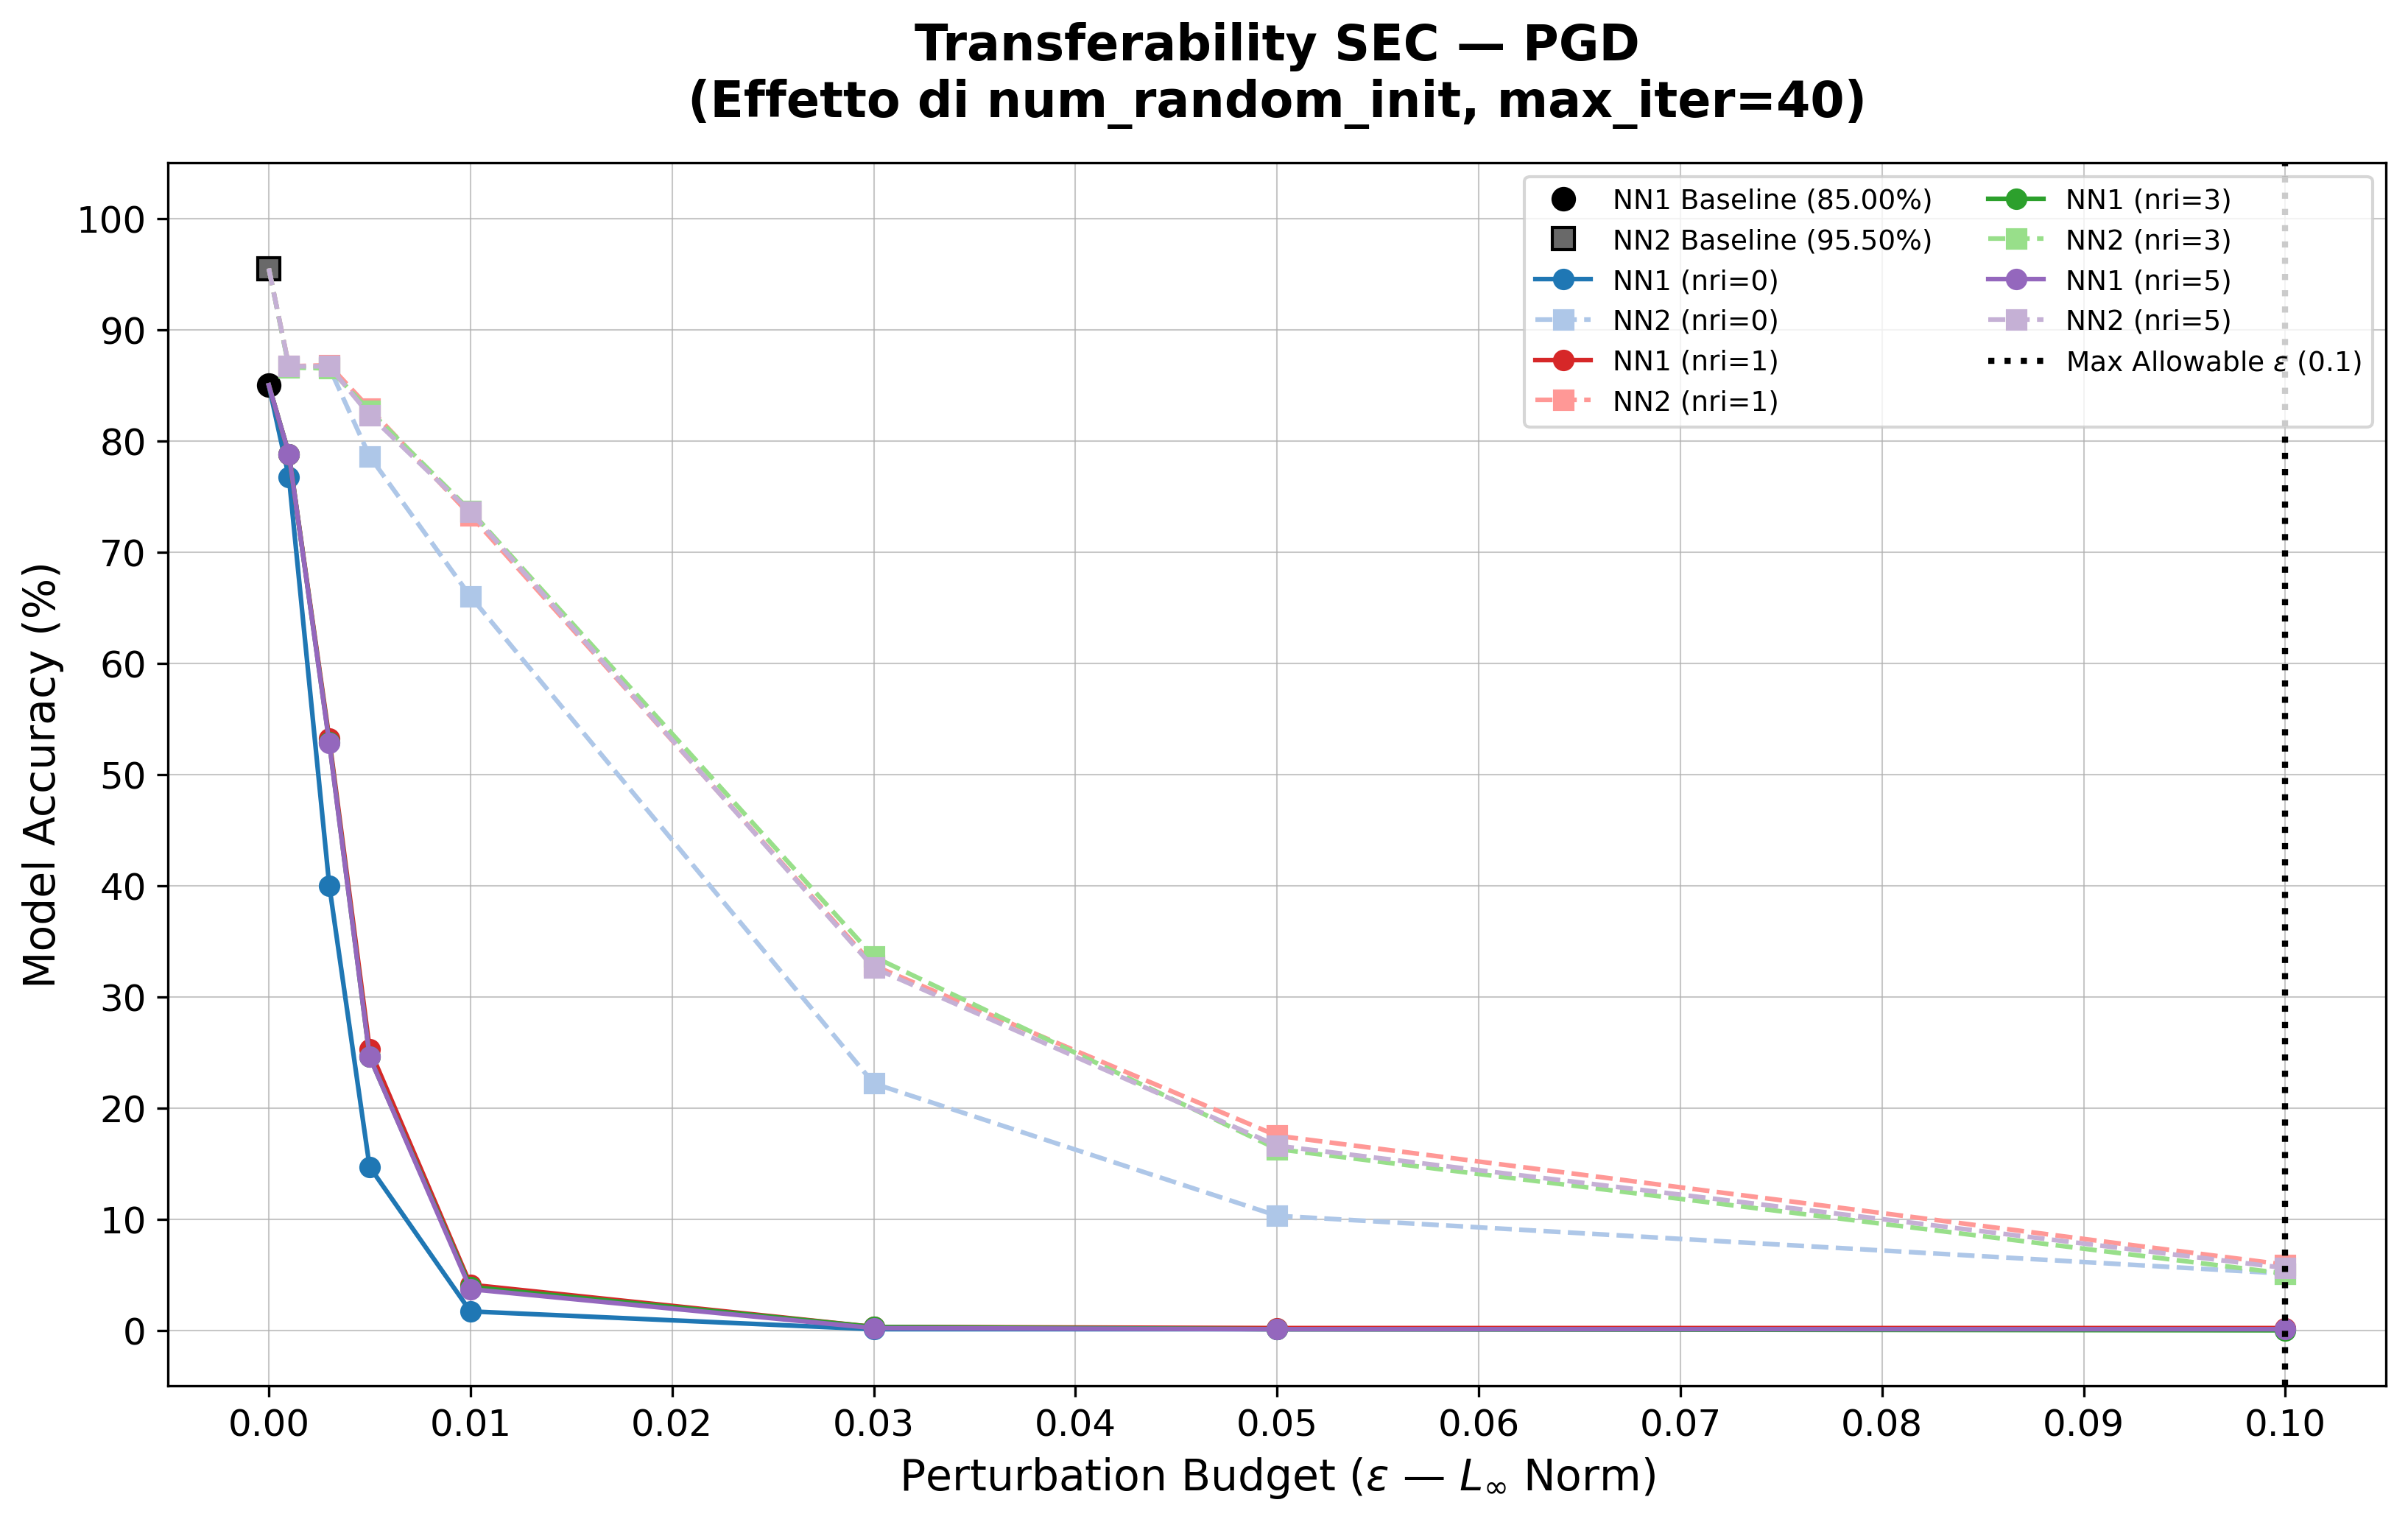
\includegraphics[width=0.85\textwidth]{./Transferability/untargeted/PGD/image1.png}
    \caption{SEC comparativa per l'attacco PGD al variare di \texttt{nri} 
    (\texttt{max\_iter} = 40).}
    \label{fig:pgd_transferability_untargeted}
\end{figure}

Dall'analisi della Figura~\ref{fig:pgd_transferability_untargeted}, emergono le 
seguenti considerazioni.
\begin{itemize}
    \item Indipendentemente dal valore di 
    \texttt{nri}, l'accuratezza del modello surrogato NN1 crolla rapidamente, 
    azzerandosi quasi completamente già per $\epsilon \geq 0.01$. 

    \item L'introduzione della random initialization riduce la transferibilità dell'attacco. La curva 
    di NN2 per \texttt{nri=0} (equivalente a BIM) si colloca sistematicamente al 
    di sotto delle curve con \texttt{nri} $\geq 1$, indicando che senza 
    inizializzazione casuale l'attacco si trasferisce con maggiore efficacia su NN2.

    \item L'incremento di \texttt{nri} oltre 
    il valore $1$ non produce miglioramenti apprezzabili. Le curve di NN2 per 
    \texttt{nri} pari a $1$, $3$ e $5$ risultano pressoché sovrapposte, 
    suggerendo che è sufficiente una singola inizializzazione casuale per 
    ottenere il massimo beneficio in termini di riduzione della transferibilità.
\end{itemize}


\begin{figure}[htbp]
    \centering
    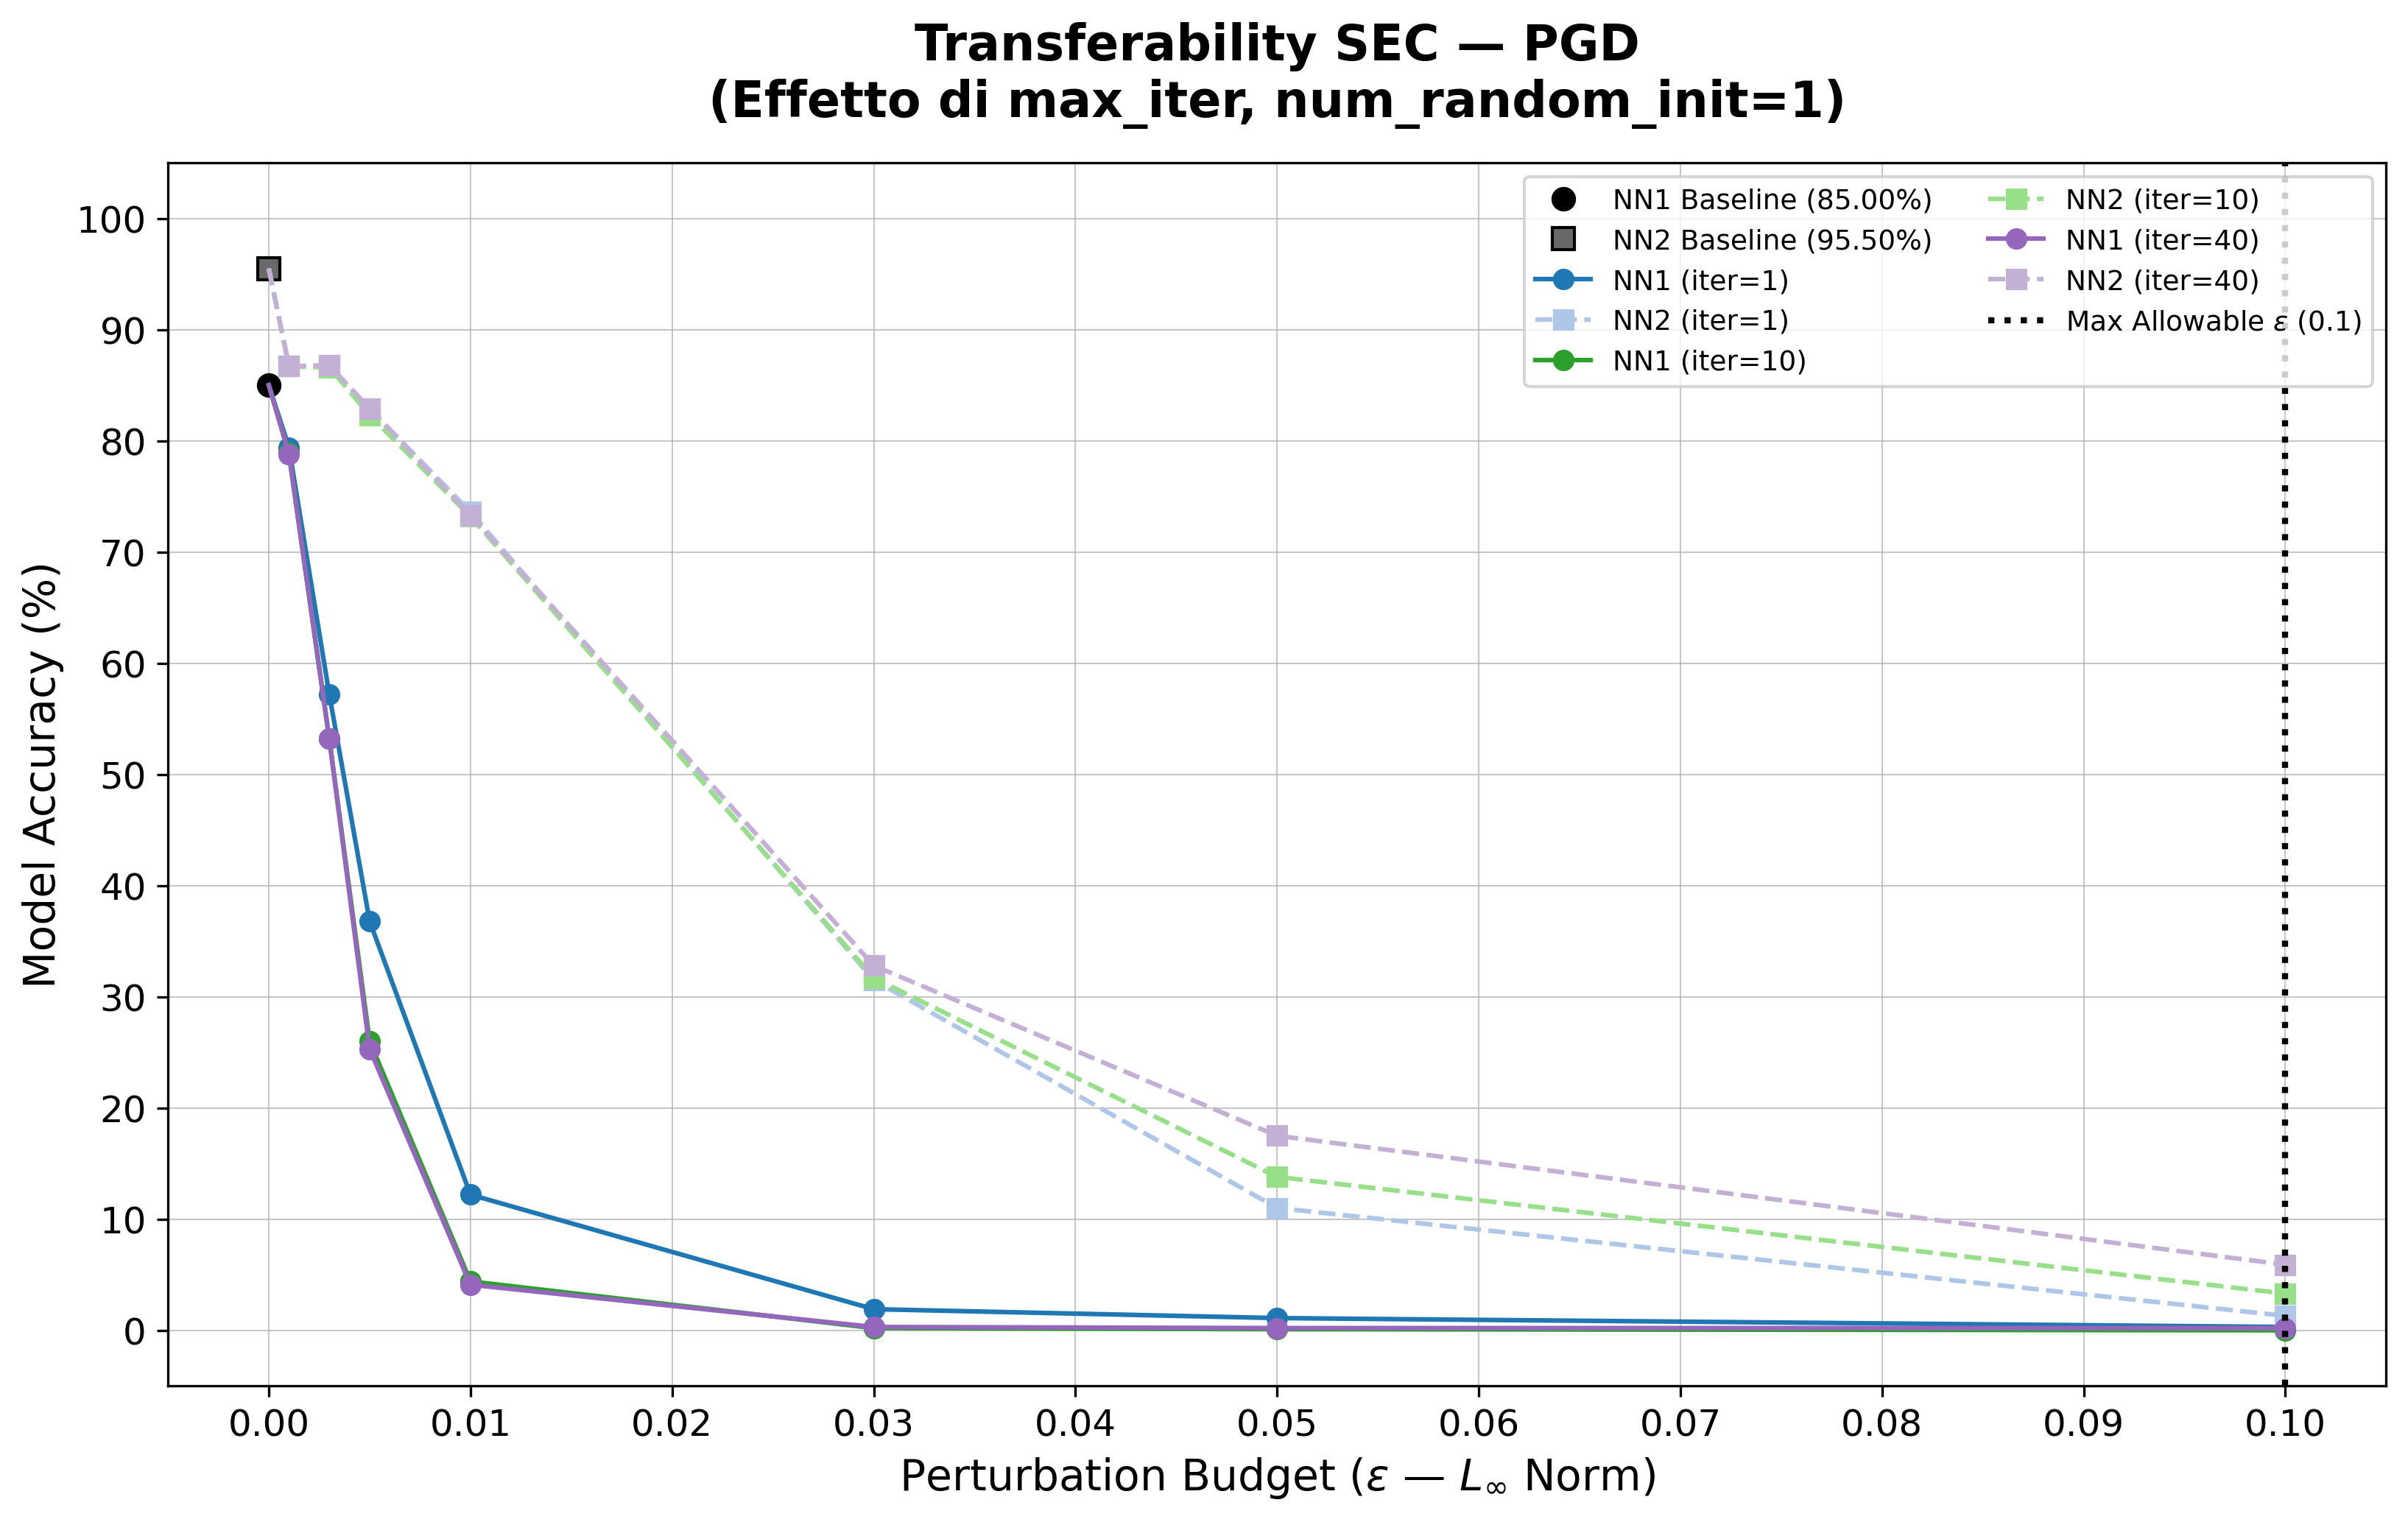
\includegraphics[width=0.85\textwidth]{./Transferability/untargeted/PGD/image2.png}
    \caption{SEC comparativa per l'attacco PGD al variare di \texttt{max\_iter} 
    (\texttt{nri} = 1).}
    \label{fig:pgd_transferability_maxiter}
\end{figure}

La seconda Security Evaluation Curve, riportata in 
Figura~\ref{fig:pgd_transferability_maxiter}, isola invece l'effetto del numero 
di iterazioni \texttt{max\_iter}, fissando $\texttt{nri}=1$, 
sufficiente (come osservato in precedenza) a sfruttare il beneficio della 
random initialization. Vengono confrontate le accuratezze di NN1 e NN2 per 
\texttt{max\_iter} pari a $1$, $10$ e $40$.

Dall'analisi della Figura~\ref{fig:pgd_transferability_maxiter}, emergono le 
seguenti considerazioni.
\begin{itemize}
    \item L'accuracy di NN2 cresce all'aumentare di \texttt{max\_iter}: 
    le curve relative a \texttt{max\_iter=40} si collocano sopra quelle con 
    \texttt{max\_iter=1}. Questo indica che un numero più elevato di iterazioni 
    riduce la transferibilità dell'attacco, in modo analogo a quanto osservato 
    per l'attacco BIM.

    \item L'effetto delle iterazioni è tuttavia graduale e contenuto: 
    l'incremento di accuratezza di NN2 tra \texttt{max\_iter=1} e 
    \texttt{max\_iter=40} si mantiene su pochi punti percentuali, a conferma che la transferibilità dell'attacco PGD è solo marginalmente influenzata dal numero di iterazioni.
\end{itemize}


\begin{table}[htbp]
    \centering
    \vspace{0.2cm}
    \setlength{\tabcolsep}{12pt}      % aumenta lo spazio orizzontale tra le colonne
    \makebox[\textwidth][c]{
    \begin{tabular}{c | ccc | ccc | ccc}
        \hline
        & \multicolumn{3}{c|}{\textbf{max\_iter = 1}}
        & \multicolumn{3}{c|}{\textbf{max\_iter = 10}}
        & \multicolumn{3}{c}{\textbf{max\_iter = 40}} \\
        \hline
        \textbf{$\epsilon$}
        & \textbf{NN1} & \textbf{NN2} & \textbf{Gap}
        & \textbf{NN1} & \textbf{NN2} & \textbf{Gap}
        & \textbf{NN1} & \textbf{NN2} & \textbf{Gap} \\
        \hline
        0.010 & 12.2\% & 73.6\% & +61.4\% & 4.4\% & 73.2\% & +68.8\% & 4.1\% & 73.3\% & +69.2\% \\
        0.030 &  1.9\% & 31.5\% & +29.6\% & 0.2\% & 31.7\% & +31.5\% & 0.3\% & 32.8\% & +32.5\% \\
        0.050 &  1.1\% & 11.0\% &  +9.9\% & 0.1\% & 13.8\% & +13.7\% & 0.2\% & 17.5\% & +17.3\% \\
        0.100 &  0.3\% &  1.3\% &  +1.0\% & 0.0\% &  3.3\% &  +3.3\% & 0.2\% &  5.9\% &  +5.7\% \\
        \hline
    \end{tabular}
    }
    \caption{Risultati di transferabilità per l'attacco PGD al variare di \texttt{max\_iter} (\texttt{nri} = 1).}
    \label{tab:pgd_maxiter_transferability}
\end{table}


Si osserva in Tabella \ref{tab:pgd_maxiter_transferability} che, a parità di $\epsilon$, il Gap tende ad aumentare con il numero 
di iterazioni. Infatti, con il crescere del numero di iterazioni, l'attacco diventa più aggressivo su NN1 ma meno trasferibile su NN2.
Con più iterazioni, infatti, la perturbazione viene ottimizzata in modo sempre 
più specifico su NN1, diventando però troppo legata a quest'ultimo per riuscire 
a ingannare anche NN2. Lo stesso comportamento era già emerso nell'analisi 
dell'attacco BIM.

Analizzando invece l'andamento lungo $\epsilon$, il Gap si riduce 
progressivamente per perturbazioni elevate, fino a valori contenuti in 
corrispondenza di $\epsilon = 0.100$ (ad esempio $+5.7\%$ per \texttt{max\_iter=40}). 
Questo comportamento indica una \textbf{crescente transferibilità} dell'attacco: 
perturbazioni più ampie riescono a compromettere NN2 favorendo la transferibilità dell'attacco.



\subsubsection{DeepFool}
In questa sezione viene valutata l'accuracy del modello NN2 sugli esempi 
avversariali generati tramite l'attacco DeepFool contro NN1, analizzandone il 
comportamento al variare del numero di iterazioni \texttt{max\_iter}. In particolare,
utilizziamo le immagini avversariali generate a partire dal test set dataset\_1\_per\_person.

I risultati sono presentati in Figura~\ref{fig:deepfool_transferability_untargeted} 
attraverso un grafico a barre che confronta, per ciascun valore di 
\texttt{max\_iter}, l'accuracy del modello surrogato NN1 e quella del modello 
bersaglio NN2 sugli stessi esempi avversariali.

\begin{figure}[htbp]
    \centering
    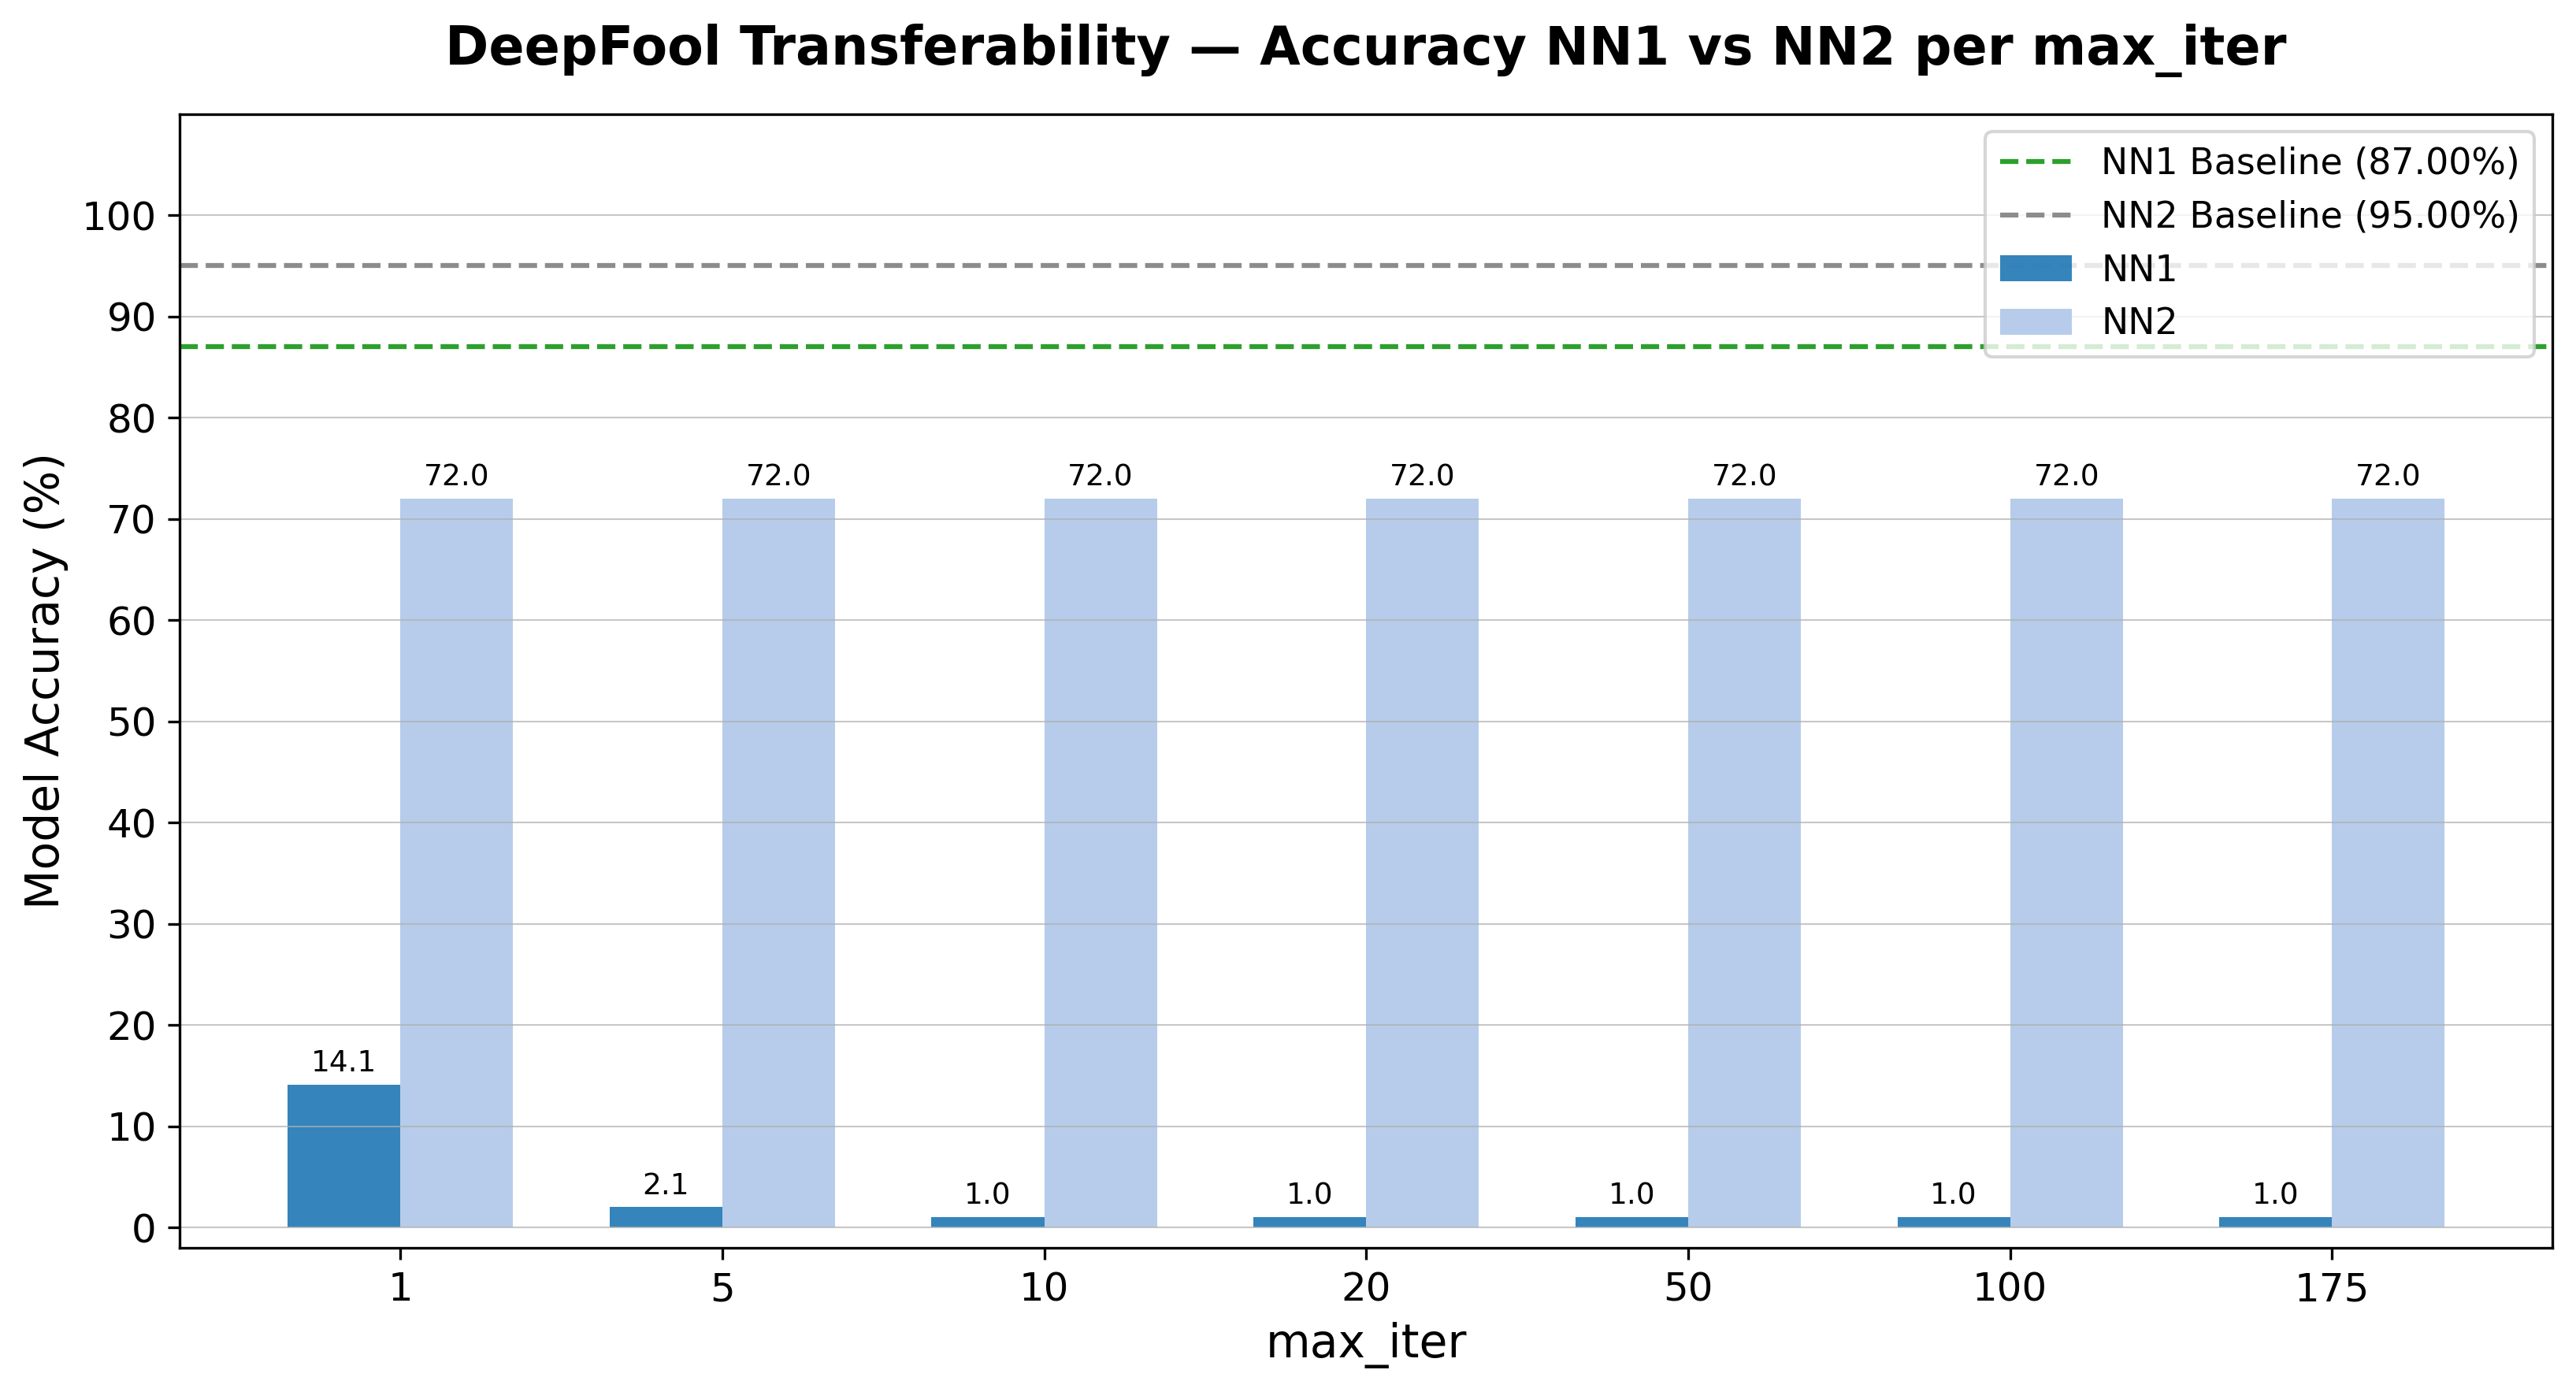
\includegraphics[width=0.85\textwidth]{./Transferability/untargeted/DeepFool/image.png}
    \caption{Confronto dell'accuracy di NN1 e NN2 per l'attacco DeepFool al 
    variare di \texttt{max\_iter}.}
    \label{fig:deepfool_transferability_untargeted}
\end{figure}

Dall'analisi della Figura~\ref{fig:deepfool_transferability_untargeted}, emergono 
le seguenti considerazioni.
\begin{itemize}
    \item L'accuracy del modello surrogato NN1 crolla rapidamente già con 
    poche iterazioni, passando dal $14.14\%$ con \texttt{max\_iter=1} all'$1.04\%$ 
    a partire da \texttt{max\_iter=10}, valore oltre il quale rimane costante. 
    Questo conferma l'elevata efficacia di DeepFool su NN1.

    \item L'accuracy del modello NN2 si mantiene costante al 
    $72.00\%$ per qualunque valore di \texttt{max\_iter}, evidenziando una
    \textbf{transferibilità molto bassa}: gli esempi avversariali, pur 
    compromettendo NN1, risultano quasi del tutto inefficaci su NN2.

    \item Il comportamento dell'attacco si stabilizza a partire da 
    \texttt{max\_iter=10}: incrementare ulteriormente il numero di iterazioni non 
    produce alcun effetto né su NN1 né su NN2, poiché DeepFool ha già raggiunto 
    la perturbazione minima necessaria a oltrepassare il confine decisionale.
\end{itemize}

La ridotta transferibilità di DeepFool trova spiegazione nell'entità delle 
perturbazioni introdotte, riportate nella 
Tabella~\ref{tab:deepfool_mean_linf}. Il Transfer Gap, calcolato come $\text{Acc}_{NN2} - \text{Acc}_{NN1}$, si mantiene 
elevato e prossimo al $+71\%$ per tutte le configurazioni, a conferma quantitativa 
della scarsa capacità dell'attacco di trasferirsi sul modello bersaglio. Per sua natura, DeepFool genera 
perturbazioni di ampiezza minima, appena sufficienti a far attraversare 
all'immagine il confine decisionale di NN1. Tali perturbazioni risultano quindi 
estremamente specifiche per il modello surrogato e, essendo di entità così 
contenuta, non sono in grado di alterare in maniera significativa la classificazione di un modello 
diverso come NN2.

\begin{table}[htbp]
    \centering
    \vspace{0.2cm}
    \small
    \setlength{\tabcolsep}{6pt}
    \renewcommand{\arraystretch}{1.1}
    \begin{tabular}{ccccc}
        \toprule
        \textbf{max\_iter} & \textbf{Accuracy NN1} & \textbf{Accuracy NN2} & \textbf{Gap} & \textbf{Mean $L_\infty$} \\
        \midrule
        1   & 14.14\% & 72.00\% & +57.86\% & 0.0442 \\
        5   &  2.06\% & 72.00\% & +69.94\% & 0.0473 \\
        10  &  1.04\% & 72.00\% & +70.96\% & 0.0471 \\
        20  &  1.04\% & 72.00\% & +70.96\% & 0.0471 \\
        50  &  1.04\% & 72.00\% & +70.96\% & 0.0471 \\
        100 &  1.04\% & 72.00\% & +70.96\% & 0.0470 \\
        175 &  1.04\% & 72.00\% & +70.96\% & 0.0471 \\
        \bottomrule
    \end{tabular}
    \caption{Risultati di transferabilità per l'attacco DeepFool al variare di \texttt{max\_iter}.}
    \label{tab:deepfool_mean_linf}
\end{table}


\subsubsection{Carlini \& Wagner}
In questa sezione viene valutata l'accuracy del modello NN2 sugli esempi 
avversariali generati tramite l'attacco Carlini \& Wagner contro NN1, 
nella sua variante \textit{untargeted}. Il comportamento dell'attacco viene 
analizzato al variare del numero di iterazioni \texttt{max\_iter} e del 
\texttt{learning\_rate}.


\begin{table}[htbp]
    \centering
    \vspace{0.2cm}
    \small
    \setlength{\tabcolsep}{8pt}
    \renewcommand{\arraystretch}{1.2}
    \begin{tabular}{cc ccc c}
        \toprule
        \textbf{learning\_rate} & \textbf{max\_iter} 
        & \textbf{Acc. NN1} & \textbf{Acc. NN2} & \textbf{Gap} 
        & \textbf{Mean $L_\infty$} \\
        \midrule
        \multirow{4}{*}{0.01}
            & 1   & 28.0\% & 84.0\% & +56.0\% & 0.0038 \\
            & 5   &  4.0\% & 84.0\% & +80.0\% & 0.0064 \\
            & 10  &  4.0\% & 84.0\% & +80.0\% & 0.0064 \\
            & 20  &  4.0\% & 84.0\% & +80.0\% & 0.0064 \\
        \midrule
        \multirow{4}{*}{0.1}
            & 1   &  2.0\% & 12.0\% & +10.0\% & 0.0500 \\
            & 5   &  2.0\% & 12.0\% & +10.0\% & 0.0500 \\
            & 10  &  2.0\% & 13.0\% & +11.0\% & 0.0500 \\
            & 20  &  2.0\% & 12.0\% & +10.0\% & 0.0500 \\
        \bottomrule
    \end{tabular}
    \caption{Risultati di transferabilità per l'attacco C\&W Untargeted al variare 
    di \texttt{learning\_rate} e \texttt{max\_iter}.}
    \label{tab:cw_transferability}
\end{table}

Dall'analisi della Tabella~\ref{tab:cw_transferability} emerge che il parametro 
determinante per la transferibilità dell'attacco C\&W è il \texttt{learning\_rate}, 
che controlla l'ampiezza della perturbazione applicata.

Con un \texttt{learning\_rate} ridotto ($0.01$), l'attacco genera perturbazioni 
molto contenute (Mean $L_\infty \approx 0.006$): NN1 viene compromesso quasi 
completamente (accuratezza al $4\%$), ma NN2 mantiene un'accuratezza elevata, 
pari all'$84\%$. Il Transfer Gap raggiunge in questo caso il $+80\%$, indicando 
una \textbf{bassa transferibilità}. Le perturbazioni, essendo di entità minima e 
specifiche per il modello surrogato, non riescono a trasferirsi su NN2, 
analogamente a quanto osservato per DeepFool.

Con un \texttt{learning\_rate} più elevato ($0.1$), la perturbazione media cresce 
di quasi un ordine di grandezza (Mean $L_\infty = 0.05$). In questo regime non 
solo NN1, ma anche NN2 viene compromesso in modo significativo, con un'accuratezza 
che scende al $12\%$ e un Transfer Gap che si riduce al $+10\%$. La maggiore 
ampiezza della perturbazione si traduce quindi in una \textbf{transferibilità 
nettamente superiore}.

Il numero di iterazioni \texttt{max\_iter} ha invece un impatto marginale: a 
parità di \texttt{learning\_rate}, i risultati si stabilizzano già a partire da 
\texttt{max\_iter=5} e rimangono sostanzialmente invariati per valori superiori. 
L'unica variazione apprezzabile si registra con \texttt{learning\_rate=0.01} nel 
passaggio da \texttt{max\_iter=1} a \texttt{max\_iter=5}, oltre il quale l'attacco 
raggiunge la sua configurazione stabile.







\subsection{Error-Specific Attack}
In questa sezione viene analizzata la transferibilità degli attacchi in modalità 
\textit{error-specific}. Si tratta quindi di un obiettivo più ambizioso e, di norma, più difficile da 
raggiungere.

Coerentemente con questo diverso obiettivo, la metrica di valutazione utilizzata 
non è più l'accuracy, bensì l'\textbf{Attack Success Rate (ASR)}, ovvero la 
percentuale di immagini che il modello classifica effettivamente nella classe 
bersaglio desiderata. Un ASR elevato indica un attacco efficace; nel contesto 
della transferibilità, un ASR elevato su NN2 indica che l'attacco, generato 
contro NN1, riesce a forzare la classe bersaglio anche sul modello bersaglio.

In accordo agli attacchi trattati nei capitoli iniziali, vengono considerate due modalità di selezione della classe bersaglio: \textbf{Least-Likely} e \textbf{Fixed}.

\subsubsection{Fast Gradient Sign Method (FGSM)}
In questa sezione viene valutata la transferibilità dell'attacco FGSM 
\textit{error-specific}, analizzando l'ASR del modello surrogato NN1 e del modello 
bersaglio NN2 al variare di $\epsilon$, nelle due modalità Least-Likely e Fixed.

\paragraph*{Modalità Fixed}\mbox{}\\
La Figura~\ref{fig:fgsm_es_fixed} riporta la Security Evaluation Curve per la 
modalità Fixed, confrontando l'ASR di NN1 e NN2 al variare di $\epsilon$.

\begin{figure}[H]
    \centering
    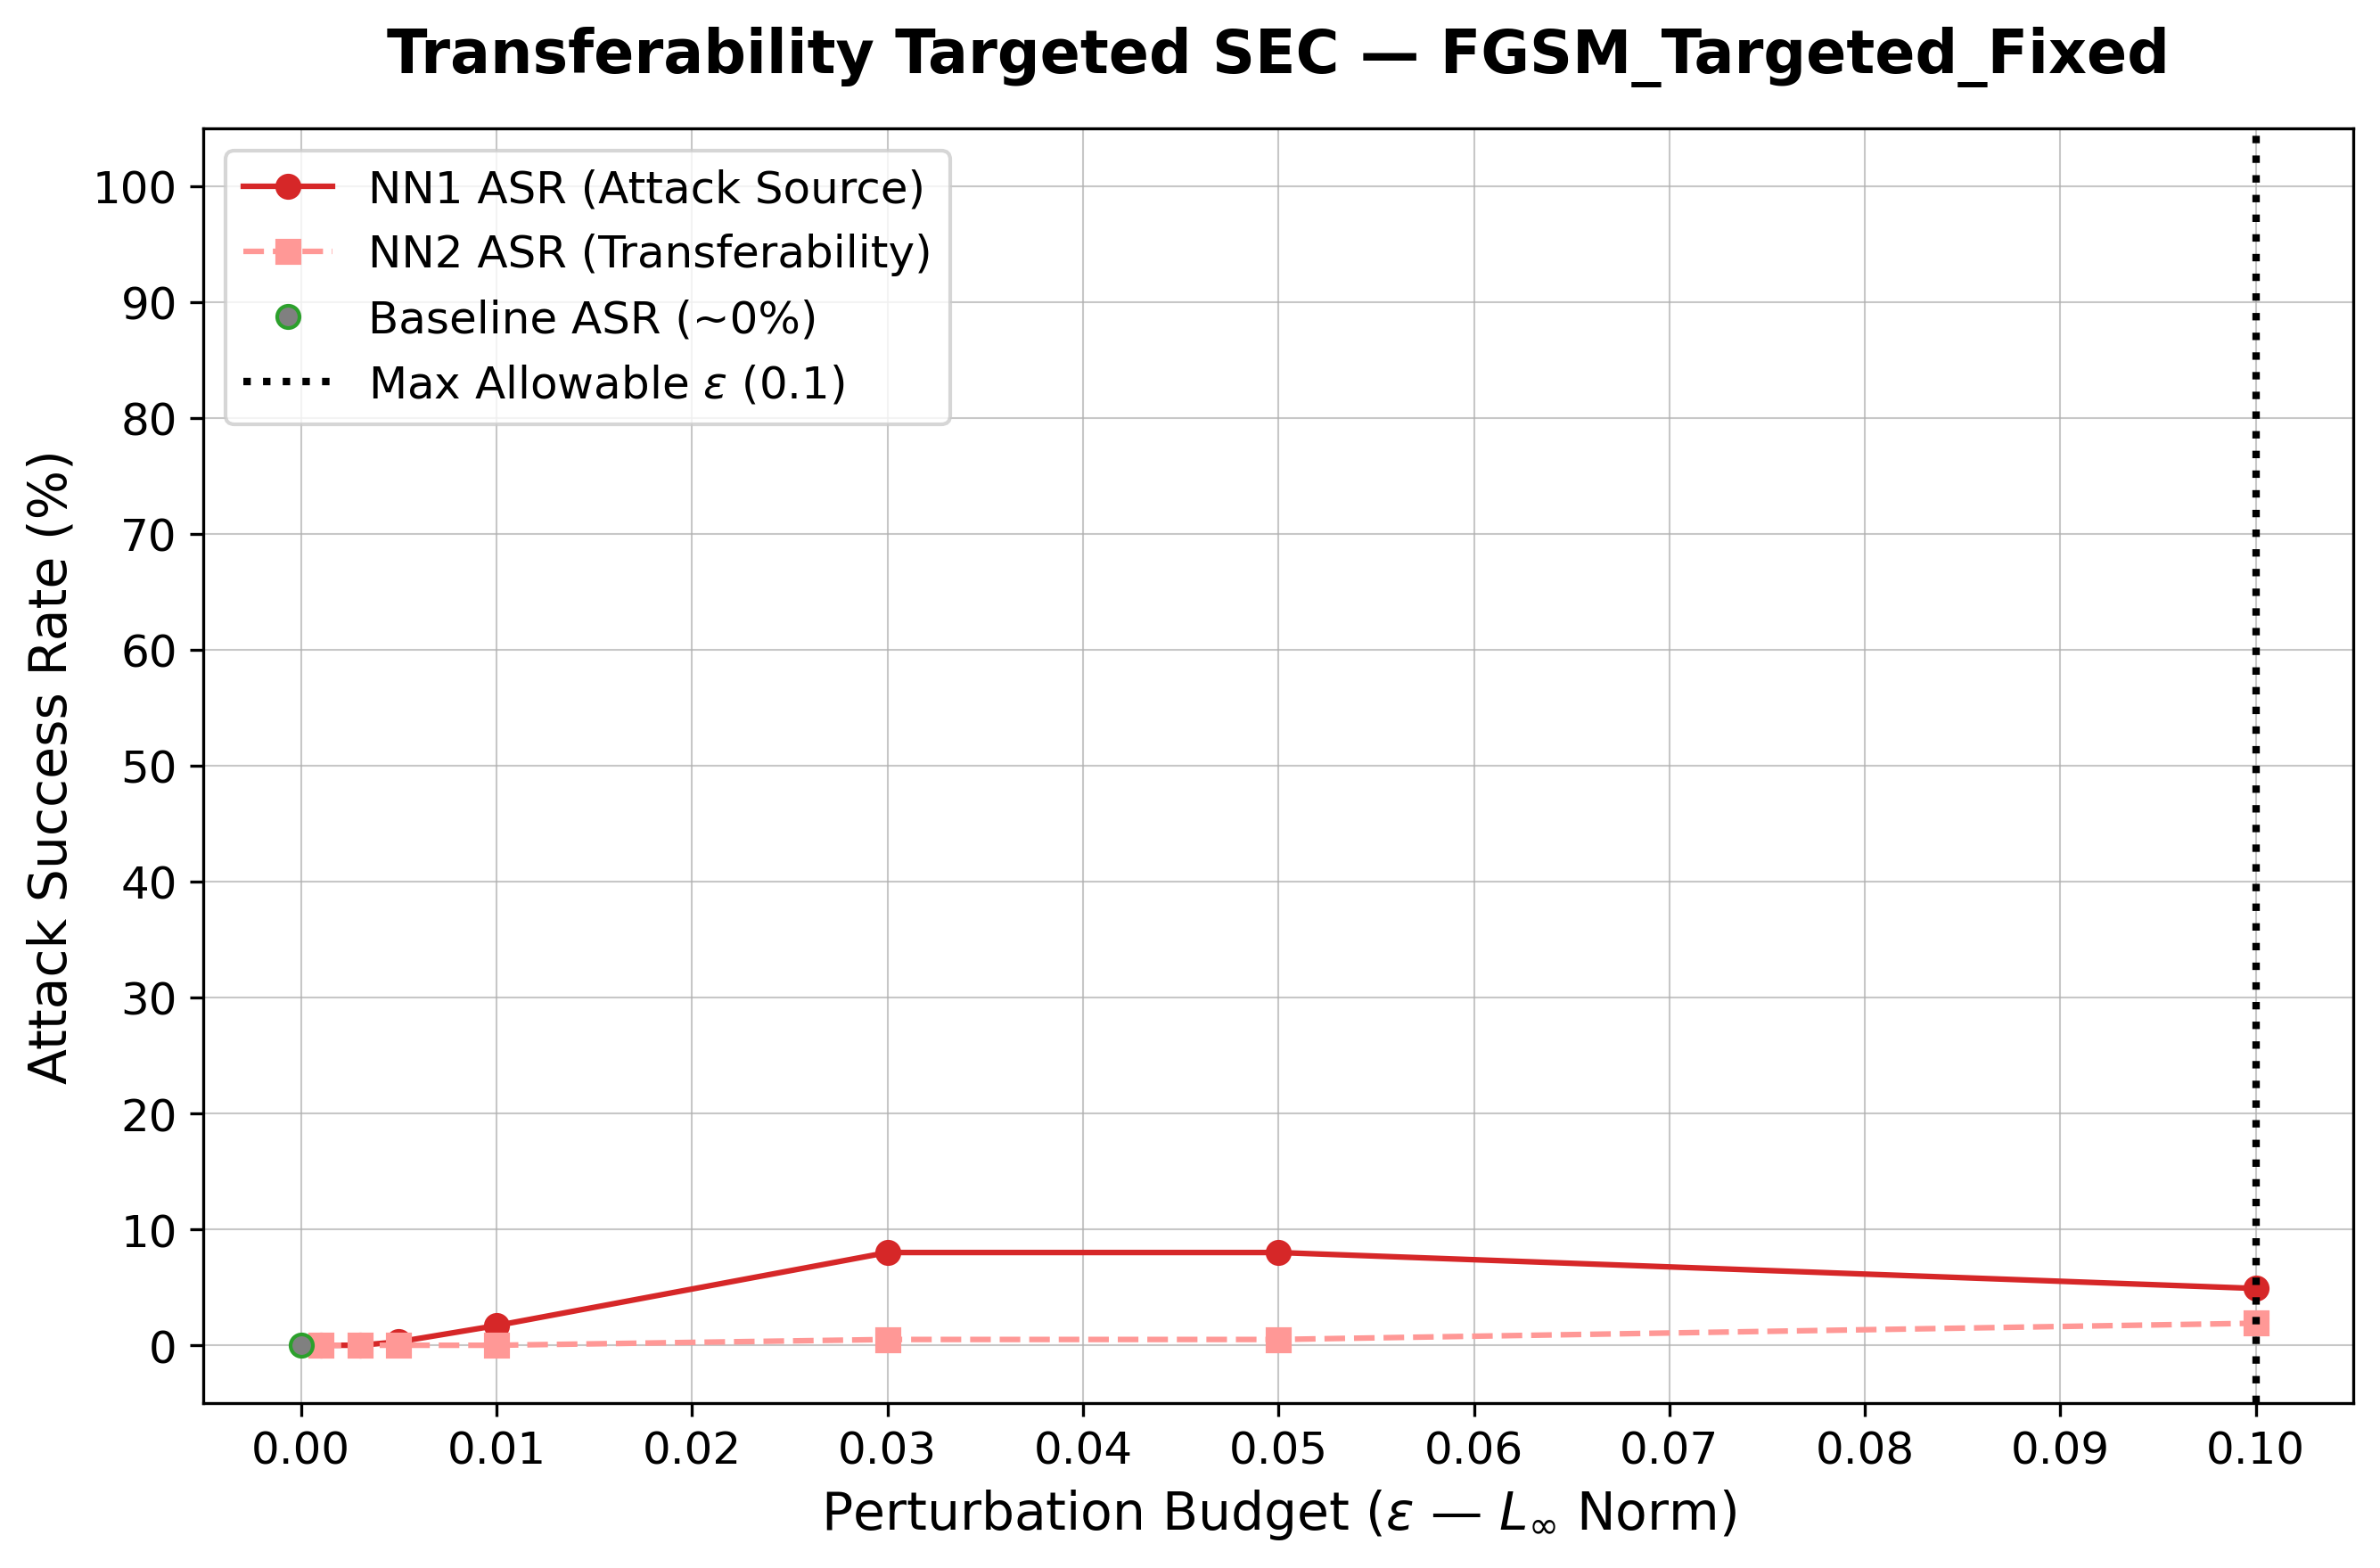
\includegraphics[width=0.8\textwidth]{./Transferability/targeted/FGSM/image_fixed.png}
    \caption{SEC comparativa per l'attacco FGSM error-specific in modalità Fixed.}
    \label{fig:fgsm_es_fixed}
\end{figure}

Dall'analisi emerge che l'ASR si mantiene molto contenuto per entrambi i modelli. 
Su NN1 l'attacco raggiunge un valore massimo dell'$8.0\%$ in corrispondenza di 
$\epsilon = 0.03$–$0.05$, per poi ridursi a $\epsilon = 0.1$. Su NN2 l'ASR resta 
quasi sempre nullo, raggiungendo al più l'$1.9\%$ per $\epsilon = 0.1$. 
L'attacco error-specific, nella sua formulazione a singolo passo, risulta quindi 
poco efficace già su NN1 e sostanzialmente \textbf{non trasferibile} su NN2.

\paragraph*{Modalità Least-Likely}\mbox{}\\
La Figura~\ref{fig:fgsm_es_ll} riporta la Security Evaluation Curve per la 
modalità Least-Likely.

\begin{figure}[htbp]
    \centering
    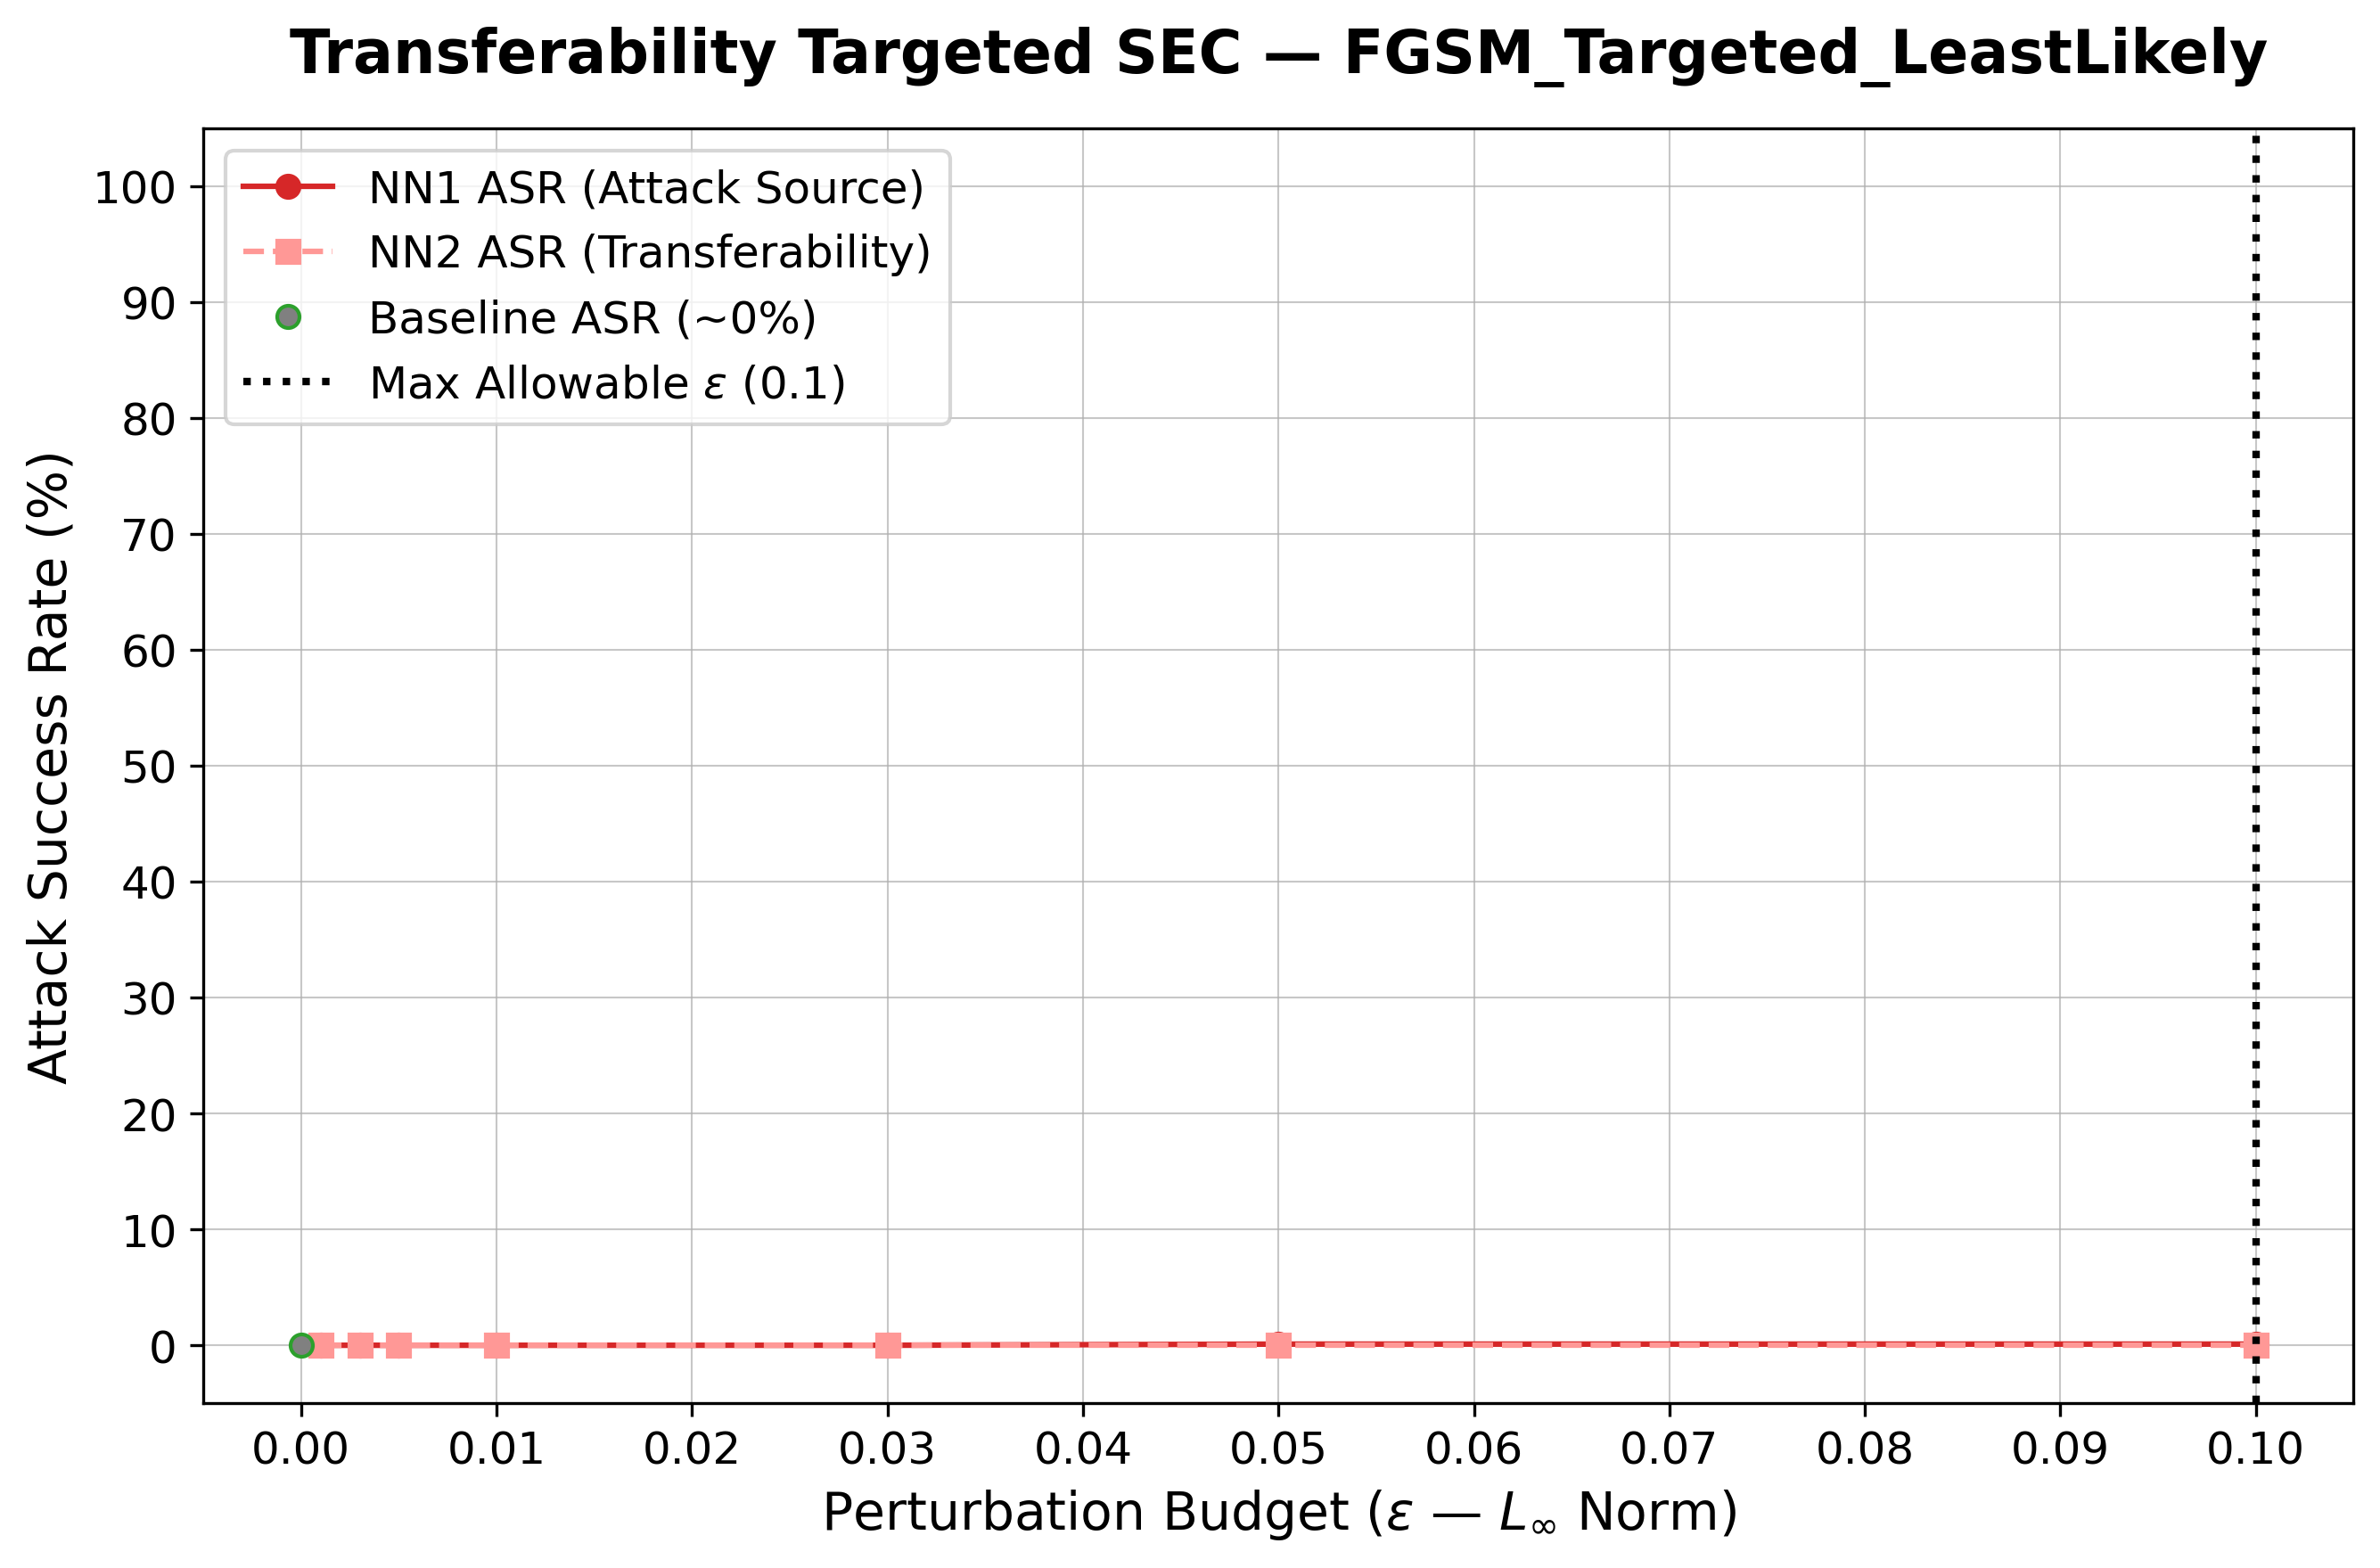
\includegraphics[width=0.8\textwidth]{./Transferability/targeted/FGSM/image_leastlikely.png}
    \caption{SEC comparativa per l'attacco FGSM error-specific in modalità 
    Least-Likely.}
    \label{fig:fgsm_es_ll}
\end{figure}

In questa modalità l'attacco risulta ancora meno efficace: l'ASR di NN1 non supera 
mai lo $0.1\%$ e quello di NN2 rimane costantemente nullo per ogni valore di 
$\epsilon$. Questo risultato è atteso: forzare la classificazione verso la classe 
\textit{meno probabile} è l'obiettivo più arduo, e un attacco a singolo passo come 
FGSM non dispone della capacità di ottimizzazione necessaria a raggiungerlo, né su 
NN1 né, tantomeno, su NN2.



\subsubsection{Basic Iterative Method (BIM)}

\subsubsection{Projected Gradient Descent (PGD)}


\subsubsection{DeepFool}


\subsubsection{Carlini \& Wagner}







\clearpage
\bibliographystyle{plain} 
\bibliography{bibliografia}
\end{document}
